\documentclass[a4paper,cleardoubleempty,BCOR1cm]{scrbook}

% use to waste space:
% \documentclass[12pt,a4paper]{article}

% if you have this style and like it.
%\documentclass{acmsiggraph}
%\documentclass[review]{acmsiggraph}      % review
%\documentclass[widereview]{acmsiggraph}  % wide-spaced review
%\documentclass[preprint]{acmsiggraph}    % preprint

% Recommended, but optional, packages for figures and better typesetting:
\usepackage{microtype}
\usepackage[pdftex]{graphicx}
\usepackage[pdftex]{color}
\definecolor{rot}{RGB}{165,30,55} %rote Farbe
\graphicspath{{./figures/}}
% \usepackage{subfigure}
\usepackage{subfig}
% \usepackage{subcaption}
\usepackage{amsmath}
\usepackage{amssymb}
\usepackage{booktabs} % for professional tables
\usepackage{textcomp}
\usepackage{todonotes}
%\usepackage{xcolor}
\usepackage{tikz}
\usepackage{amsthm}
\usepackage{hyperref}

\usepackage{cleveref}


\usepackage{mathptmx}
\usepackage{parskip}
%\usepackage{amsmath}
\usepackage{dsfont}
\usepackage{pxfonts}

\usepackage[T1]{fontenc}
\usepackage{textcomp}
\usepackage{tabularx}
\usepackage{booktabs}

%\usepackage{float} %for nicer figure placement
\usepackage[section]{placeins}

%plots
\usepackage{caption}
\usepackage{pgfplots}
\pgfplotsset{compat=newest}

\newlength{\figwidth}
\newlength{\figheight}

\newlength{\tempheight}
\newlength{\tempwidth}

\newcommand{\rowname}[1]% #1 = text
{\rotatebox{90}{\makebox[\tempheight][c]{\textbf{#1}}}}

\setlength{\tempwidth}{.3\linewidth}

\setlength{\figwidth}{0.8\textwidth}
\setlength{\figheight}{0.3\textheight}

\newtheorem{proposition}{Proposition}

\usepgfplotslibrary{groupplots}
\usepgfplotslibrary{dateplot}


% comment these two lines out if you don't want minion/myriad fonts.
% \usepackage[minionint,mathlf]{MinionPro}
% \renewcommand{\sfdefault}{Myriad-LF}
%\usepackage{Myriad}

\usepackage{geometry}
\newcommand{\squeezeup}{\vspace{-20mm}}

%\usepackage{apalike}
%\let\bibhang\relax
\usepackage{natbib}
%\bibliographystyle{apa}

\bibliographystyle{rusnat}

%\usepackage{natbib}		% textual referencing
%\usepackage[numbers,super]{natbib}	% nice superscripts
%\bibliographystyle{chicago}	% shitty
%\bibliographystyle{alpha}	% abbr names and year in \cite
%\bibliographystyle{agsm}	% australian, need natbib
%\bibliographystyle{kluwer}	% need natbib
%\bibliographystyle{apalike}	% lengthly
%\bibliographystyle{abbrv}	% minimal?
%\bibliographystyle{icml2020}

% use for german line breaking:
%\usepackage[ngerman]{babel}
\usepackage[T1]{fontenc}
\usepackage[utf8x]{inputenc}

% avoid us-style text color destruction:
\frenchspacing
\usepackage{microtype}
\usepackage{setspace} 

% have a nice framebox with border directly around the image:
\fboxsep 0pt
\newcommand{\fimg}[2]{\fbox{\includegraphics[width=#1]{#2}}}

%\usepackage{theorem}
%\theorembodyfont{\upshape}
%\newtheorem{definition}{Definition}
\usepackage{listings}
%\usepackage[boxruled]{algorithm2e}

\usepackage{algorithm}
\usepackage{algorithmic}

\renewcommand{\algorithmicrequire}{\textbf{Input:}}
\renewcommand{\algorithmicensure}{\textbf{Output:}}
\renewcommand{\algorithmiccomment}[1]{\bgroup\hfill\scriptsize\it//~#1\egroup}
\newcommand{\algorithmicbreak}{\textbf{break}}
\newcommand{\BREAK}{\STATE \algorithmicbreak}

\usepackage{url}
\usepackage{subfig}
\usepackage{arydshln} %for dashed lines
\usepackage{fancyhdr} %for fancy head and foot design
%captionbefehle einbingen
\usepackage{caption} 
\captionsetup{labelfont=bf, font={small,sf}}
\def\code#1{{\tt{#1}}}



\title{Fast Predictive Uncertainty for Classification with Bayesian Deep Networks}
\author{Marius Hobbhahn \thanks{e-mail: marius.hobbhahn@student.uni-tuebingen.de}}
\date{\today}

\input{math_commands}


\begin{document}

\newpage	
\begin{tabular}{lr}
% \includegraphics[width=0.5\linewidth]{logo_sw} % logo bw
 \includegraphics[width=0.5\linewidth]{UT_WBMW_Rot_4C} % logo red
 & \hspace{0.2\linewidth}
 \parbox{0.5\linewidth}{
   \large\bf\textsf{\color{rot}{Mathematisch-\\Naturwissenschaftliche\\Fakultät\\\\}}
  \hspace{-.144cm}\normalsize\textsf{\color{rot}{Methoden des Maschinellen Lernens}}
   \vspace{0.6cm}
 }
\end{tabular}

\vspace*{10ex}
Masterarbeit

{\huge\bf\textsf{Fast Predictive Uncertainty for Classification with Bayesian Deep Networks}}

\vspace*{30ex}

Eberhard Karls Universität Tübingen\\
Mathematisch-Naturwissenschaftliche Fakultät\\
Wilhelm-Schickard-Institut für Informatik\\
Methoden des Maschinellen Lernens\\
Marius Hobbhahn,~ \verb+marius.hobbhahn@student.uni-tuebingen.de+,~ 2019/20

\vspace*{5ex}

\begin{tabular}{@{}l@{\hspace{2em}}l}
  Bearbeitungszeitraum:& vom 20.02.20 bis 20.06.20 \vspace*{5ex} \\
  Betreuer/Gutachter:& Prof. Dr. Philipp Hennig, Universität Tübingen\\
  Zweitgutachter:& Prof. Dr. Zeynep Akata, Universität Tübingen
\end{tabular}

\thispagestyle{empty}
\newpage

\chapter*{Selbstst\"andigkeitserkl\"arung}

Hiermit erkl\"are ich, dass ich diese schriftliche Abschlussarbeit selbst\"andig verfasst habe,
keine anderen als die angegebenen Hilfsmittel und Quellen benutzt habe und alle w\"ortlich
oder sinngem\"aß aus anderen Werken übernommenen Aussagen als solche gekennzeichnet
habe. \\

\vspace*{8ex}
\hrule
\vspace*{2ex}
Marius Hobbhahn (Matrikelnummer 4003731), \today

\newpage

\onehalfspacing % zeilen abstand 1.5

\pagestyle{fancy}
\fancyhf{}
%\fancyhead[LE,RO]{\leftmark}   %current chapter and section on the outer side header
%\fancyhead[RE,LO]{\thechapter}
%\fancyfoot[CE,CO]{\rightmark}  %next chapter and section in the center bot
\fancyfoot[LE,RO]{\thepage}  %page number on the outer bottom side

\section*{Abstract}

In Bayesian Deep Learning, distributions over the output of classification neural networks are approximated by first constructing a Gaussian distribution over the weights, then sampling from it to receive a distribution over the categorical output distribution. This is costly. We reconsider old work to construct a Dirichlet approximation of this output distribution, which yields an analytic map between Gaussian distributions in logit space and Dirichlet distributions (the conjugate prior to the categorical) in the output space. We argue that the resulting Dirichlet distribution has theoretical and practical advantages, in particular more efficient computation of the uncertainty estimate, scaling to large datasets and networks like ImageNet and DenseNet. We demonstrate the use of this Dirichlet approximation by using it to construct a lightweight uncertainty-aware output ranking for the ImageNet setup. 



\newpage
\section*{Zusammenfassung}
Im Bayesian Deep Learning werden Verteilungen über die Ausgaben von neuronalen Netzen dadurch erzeugt, dass zunächst eine Gaussverteilung über die Gewichte konstruiert wird und aus dieser dann samples gezogen werden, welche, nach Anwendung der softmax Funktion, eine kategorische Verteilung darstellen. Das ist aufwendig. Wir nutzen altes, aber nützliches, Wissen um eine Dirichlet Approximation der Ausgabeverteilung zu konstruieren. Diese Brücke stellt eine analytische Abbildung zwischen einer Normalverteilung im logit-Raum und einer Dirichletverteilung (dem conjugate prior der Kategorischen Verteilung) im Ausgaberaum dar. Wir argumentieren, dass die resultierende Dirichletverteilung theoretische und praktische Vorteile hat. Die Berechnung der Unsicherheit bezüglich der Ausgabeverteilung ist beispielsweise wesentlich effizienter und die Methode lässt sich einfach auf große Datensätze und Netzwerke, wie ImageNet und DenseNet, hochskalieren. Wir demonstrieren diesen Fakt mit einem Unsicherheits-bewussten Ausgaberanking für ImageNet. 




\tableofcontents

%%%%% show current chapter on the top, current section and page number on the bottom %%%%
\pagestyle{fancy}
\fancyhf{}
\fancyhead[LE,RO]{\leftmark}   %current chapter and section on the outer side header
\fancyhead[RE,LO]{\thechapter}
\fancyfoot[CE,CO]{\rightmark}  %next chapter and section in the center bot
\fancyfoot[LE,RO]{\thepage}  %page number on the outer bottom side

\chapter{Introduction}
\label{chap:introduction}
Quantifying the uncertainty of neural networks' (NNs) predictions is important in safety-critical applications such as medical-diagnosis \cite{UIinMedicine} and self-driving vehicles \cite{McAllister2017ConcretePF,AutoDrivingBayes}.
Architectures for classification tasks produce a probability distribution as their output, constructed by applying the softmax to the point-estimate output of the penultimate layer.
However, it has been shown that this distribution is overconfident \citep{nguyen2015deep,Hein_2019_CVPR} and thus cannot be used for predictive uncertainty quantification.

Approximate Bayesian methods provide quantified uncertainty over the network's parameters and thus the outputs in a tractable fashion. The commonly used Gaussian approximate posterior \citep{MacKay1992,Graves2011VB,Blundell2015WeightUI,ritter2018a} approximately induces a Gaussian distribution over the logits of a NN \citep{McKay1995NetworkBayesReview}. However, the associated predictive distribution, which is the expectation of the softmax function w.r.t. the Gaussian, does not have an analytic form.
It is thus generally approximated by Monte Carlo (MC) integration requiring multiple samples. Predictions in Bayesian neural networks (BNNs) are thus generally expensive operations.

\begin{figure}[htb]
     \centering
     \subfloat{\includegraphics[width=0.4\textwidth]{figures/sMAP/sMAP_Gaussian_coolwarm_0.png}}
     \subfloat{\includegraphics[width=0.4\textwidth]{figures/sMAP/sMAP_Dirichlet_coolwarm_0.png}}

    \setcounter{subfigure}{0}

     \subfloat[Monte Carlo]{\includegraphics[width=0.4\textwidth]{figures/sMAP/sMAP_Gaussian_coolwarm_1.png}}
     \subfloat[Laplace Bridge]{\includegraphics[width=0.4\textwidth]{figures/sMAP/sMAP_Dirichlet_coolwarm_1.png}} \\
     \caption{Densities on the simplex of the true distribution (left column, computed by exhaustive sampling by mapping a Gaussian random variable through the softmax transformation) and ``Laplace Bridge'' approximation constructed in this thesis (right column). For the top and bottom rows, two different Gaussians were used, such that the resulting mode is the same, but the uncertainty differs.}
    \label{fig:LPbridge_sMAP}
\end{figure}
	
In this thesis, we re-introduce an old but largely overlooked idea originally proposed by David JC \citet{MacKay1998} in a different setting (arguably the inverse of the Deep Learning setting). Dirichlet distributions are generally defined on the simplex. But when its variable is defined on the inverse softmax's domain, its shape effectively approximates a Gaussian. The inverse of this approximation, which will be called the \emph{Laplace Bridge} here \citep{KernelTopicModels2012}, analytically maps a Gaussian distribution onto a Dirichlet distribution. Given a Gaussian distribution over the logits of a NN, one can thus efficiently obtain an approximate Dirichlet distribution over the softmax outputs (\Cref{fig:LPbridge_sMAP}). Our contributions in this thesis are: We re-visit MacKay's derivation with particular attention to a symmetry constraint that becomes necessary in our ``inverted'' use of the argument from the Gaussian to the Dirichlet family. We then validate the quality of this approximation both by theoretical and empirical arguments, and demonstrate significant speed-up over MC-integration. Finally, we show a use-case, leveraging the analytic properties of Dirichlet distributions to improve the popular top-$k$ metric through uncertainties.

To sharpen the intuition about the modifications to classical BNNs proposed by this thesis consider Figure \ref{fig:LaplaceBridge_intuition}.

\begin{figure}[htb]
	\centering
	\includegraphics[width=0.8\textwidth]{figures/GaussNN_classic.pdf} \\
	\includegraphics[width=0.8\textwidth]{figures/GaussNN_LaplaceBridge.pdf} \\
	\caption{Visualization of the modification of BNNs through the Laplace Bridge. The \textit{Parameter space} part is representative for any method that yields a Gaussian predictive posterior in the logit space. \textbf{Top:} The softmax function is applied to samples drawn from the posterior predictive Gaussian. The result is a distribution represented by samples. \textbf{Bottom:} The Laplace Bridge is applied to the posterior predictive Gaussian. The result is a parameterized Dirichlet distribution over the outputs.}
	\label{fig:LaplaceBridge_intuition}
\end{figure}

We think that the Laplace Bridge is a valuable method to estimate predictive uncertainty because it is easy to add to already existing architectures and it is very fast compared to sampling schemes. When combined with a Laplace approximation of the weights, the Laplace Bridge can use pre-trained models and is, therefore, a simple extension to existing architectures. The cost of computing the Laplace Bridge are lower than drawing one (!) sample from a Gaussian distribution over the logits and the result is a fully parameterized Dirichlet distribution over the output space. This implies that the computational cost during application is reduced to a minimum. Having fast predictive uncertainty is important because it means viability for safety-critical applications, e.g. self-driving cars where a difference of milliseconds can increase safety and be used in rapid succession for multiple hundred frames per second. 

\Cref{chap:background} provides the mathematical derivation. \Cref{chap:method} and \ref{sec:practicalities} discuss the Laplace Bridge in the context of neural networks and with a deeper analysis of different ways to do posterior inference. We compare it to the recent approximations of the predictive distributions of NNs in \Cref{chap:related_work}. Empirical experiments are presented in \Cref{chap:experiments}.


\chapter{The Laplace Bridge}
\label{chap:background}
\section{Background}
\label{sec:background}

\subsection{Change of Variable for Probability Density Function}
\label{subsec:variable_change_pdf}

%TODO reference to book
\subsubsection*{1D}
Let $X$ have a continuous density $f_X$. Let $g: \mathbb{R} \rightarrow \mathbb{R}$ be piece-wise strictly monotone and continuously differentiable, i.e. there exists intervals $I_1,I_2, ..., I_n$ which partition $\mathbb{R}$ such that $g$ is strictly monotone and continuously differentiable on the interior of each $I_i$. For each $i, g:I_i \rightarrow \mathbb{R}$ is invertible on $g(I_i)$ and let $g_i^{-1}$ be the inverse function. Let $Y = g(X)$ and $\wedge = \{y| y=g(x), x \in \mathbb{R}\}$ be the range $g$. Then the density function $f_Y$ of $Y$ exists and is given by 
\begin{equation}
\label{eq:1D_variable_transform}
f_Y(y) = \sum_{i=1}^{n} f_X(g_i^{-1}(y)) \left\vert\frac{\partial g_i^{-1}(y)}{\partial y} \right\vert \mathbf{1}_\wedge(y) 
\end{equation}

\subsubsection*{Higher dim}
TODO: Jacobian. But how do the intervals work?


\subsection{Laplace Approximation}

The Laplace approximation (LPA) is a tool to fit a normal distribution to the PDF of a given other distribution. The only constraints for the other distribution are: one peak (mode/ point of maximum) and twice differentiable. Laplace proposed a simple 2-term Taylor expansion on the log pdf. If $\hat{\theta}$ denotes the mode of a pdf $h(\theta)$, then it is also the mode of the log-pdf $q(\theta) = \log h(\theta)$. The 2-term Taylor expansion of $q(\theta)$ therefore is:

\begin{align}
	q(\theta) &\approx q(\hat{\theta}) + q'(\hat{\theta})(\theta - \hat{\theta}) + \frac{1}{2}(\theta- \hat{\theta})q''(\hat{\theta}) (\theta - \hat{\theta})\\
	&= 	q(\hat{\theta}) + 0 +  \frac{1}{2}(\theta- \hat{\theta})q''(\hat{\theta}) (\theta - \hat{\theta}) \qquad \text{[since } q'(\theta) = 0]\\
	&= c - \frac{(\theta - \mu)^2}{2\sigma^2}
\end{align}
where $c$ is a constant, $\mu = \hat{\theta}$ and $\sigma^2 = \{-q''(\hat{\theta})\}^{-1}$. The right hand side of the last line matches the log-pdf of a normal distribution $N(\mu, \sigma^2)$. Therefore the pdf $h(\theta)$ is approximated by the pdf of the normal distribution $N(\mu, \sigma^2)$ where $\mu = \hat{\theta}$ and $\sigma^2 = \{-q''(\hat{\theta})\}^{-1}$. Note, that even though this derivation is done for the one dimensional case only, it is also true for the multidimensional case. The second derivative just becomes the Hessian of the pdf at the mode.

\subsection{Exponential Family}

exponential family form

\begin{equation}
 f(x|\theta) = h(x)\exp[\eta(\theta) t(x) - A(\theta)]
 \label{eq:exp_family}
\end{equation}

for sufficient statistics $t:X \rightarrow \mathbb{R}$, natural parameters $\eta: \Theta \rightarrow \mathbb{R}$, and functions $A: \Theta \rightarrow \mathbb{R}$ and $h: X \rightarrow \mathbb{R}_+$

\subsection{Chi2 <-> Normal}
\label{subsec:chi2-normal}

%TODO reference the book where I took it from
It is already well-known that the Chi-squared distribution describes the sum of independent, standard normal random variables. To introduce a certain 'trick' we show the forward and backward transformation between chi2 and normal.\\
Let $X$ be normal with $\mu = 0, \sigma^2 = 1$. Let $Y = X^2$ and therefore $g(x) = x^2$, which is neither monotone nor injective. Take $I_1 = (-\infty, 0)$ and $I_2 = [0, +\infty)$. Then $g$ is monotone and injective on $I_1$ and $I_2$ and $I_1 \cup I_2 = \mathbb{R}$. $g(I_1) = (0, \infty)$ and $g(I_2) = [0, \infty)$. Then $g_1^{-1}: [0, \infty) \rightarrow \mathbb{R}$ by $g_1^{-1}(y) = -\sqrt{y}$ and $g_2^{-1}: [0, \infty) \rightarrow \mathbb{R}$ by $g_2^{-1}(y) = \sqrt{y}$. Then
$$\left\vert \frac{\partial g_i^{-1}(y)}{\partial y} \right\vert = \left\vert \frac{1}{2 \sqrt{y}} \right\vert = \frac{1}{2 \sqrt{y}}$$

Applying Equation \ref{eq:1D_variable_transform} we can transform a normal distribution to a chi-squared.

\begin{align}
	f_Y(y) &= f_X(g_1^{-1}(y))	\left\vert\frac{\partial g_1^{-1}(y)}{\partial y} \right\vert \mathbf{1}_\wedge(y) + f_X(g_2^{-1}(y))	\left\vert\frac{\partial g_2^{-1}(y)}{\partial y} \right\vert \mathbf{1}_\wedge(y) \nonumber\\
	&= \frac{1}{\sqrt{2\pi}} \exp(-\frac{y}{2}) \frac{1}{2\sqrt{y}} + \frac{1}{\sqrt{2\pi}} \exp(-\frac{y}{2}) \frac{1}{2\sqrt{y}} \qquad(y > 0)\\
	&= \frac{1}{\sqrt{2\pi}} \frac{1}{\sqrt{y}}\exp(-\frac{y}{2}) \nonumber
\end{align}

The 'trick' was to split up the variable transformation in two parts to adjust for the fact that the space of the chi-squared and the Normal are different. We can reverse the same procedure to get from a chi-squared to a normal distribution. We keep the variable names from before. Let $X = \sqrt{Y}$ and therefore $h(x) = \sqrt{x}$. Then $h_1^{-1}: \mathbb{R} \rightarrow (-\infty, 0)$ by $h_1^{-1}(x) = -x^2$ and $h_2^{-1}: \mathbb{R} \rightarrow [0, \infty)$ by $h_2^{-1}(x) = x^2$. Then

$$\left\vert\frac{\partial h_i^{-1}(y)}{\partial y} \right\vert = \vert 2x \vert $$

and
 
\begin{align}
	f_X(x) &= f_y(h_1^{-1}(x)) \left\vert\frac{\partial h_1^{-1}(y)}{\partial y} \right\vert \mathbf{1}_\wedge(y) + f_y(h_2^{-1}(x)) \left\vert\frac{\partial h_2^{-1}(y)}{\partial y} \right\vert \mathbf{1}_\wedge(y) \nonumber \\
	&= \frac{1}{\sqrt{2\pi}} \frac{1}{2\sqrt{x^2}} \exp(-\frac{x^2}{2}) |2x| \mathbf{1}_{(-\infty, 0)}(x) + \frac{1}{\sqrt{2\pi}} \frac{1}{2\sqrt{x^2}} \exp(-\frac{x^2}{2}) |2x| \mathbf{1}_{[0, \infty)}(x) \\
	&= \frac{1}{\sqrt{2\pi}} \exp(-\frac{x^2}{2}) \nonumber
\end{align}

which is defined on the entirety of $\mathbb{R}$.

\chapter{The Laplace Bridge for BNNs}
\label{chap:method}
%!TEX root = ../Laplace_bridge_for_NNs.tex

Let $f_\vtheta: \R^N \to \R^K$ be an $L$-layer neural network parametrized by $\vtheta \in \R^P$, with a Gaussian approximate posterior $\N(\vtheta | \vmu_\vtheta, \mSigma_\vtheta)$. For any input $\vx \in \R^N$, one way to obtain an approximate Gaussian distribution on the pre-softmax output (logit vector) $f_\vtheta(\vx) =: \vz$ is as
%
\begin{equation} \label{eq:logit_dist}
    q(\vz \vert \vx) \approx \N(\vz | \vmu_\vtheta^\top \vx, \mJ(\vx)^\top \mSigma_\vtheta \mJ(\vx)) \, ,
\end{equation}
%
where $\mJ(\vx)$ is the $P \times K$ Jacobian matrix representing the derivative $\frac{\partial \vz}{\partial \vtheta}$ \citep{McKay1995NetworkBayesReview}. Approximating the density of the softmax of this Gaussian random variable as a Dirichlet, using the Laplace Bridge, \emph{analytically} approximates the predictive distribution in a single step, as opposed to many samples. From Eq.~\eqref{eq:alpha_transform}, this requires $\mathcal{O}(K)$ computations to construct the $K$ parameters $\alpha_k$ of the Dirichlet. In contrast, MC-integration has computational costs of $\mathcal{O}(MJ)$, where $M$ is the number of samples and $J$ is the cost of sampling from $q(\vz \vert \vx)$ (typically $J$ is of order $K^2$ after an initial $\mathcal{O}(K^3)$ operation for a matrix decomposition of the covariance). The Monte Carlo approximation has the usual sampling error of $\mathcal{O}(1/\sqrt{M})$, while the Laplace Bridge has a fixed but small error (empirical comparison in \Cref{subsec:exp3_time}).

We now discuss several qualitative properties of the Laplace Bridge relevant for the uncertainty quantification use case in Deep Learning. For output classes of ``comparably high'' probability (as defined below), the variance $\mathrm{Var}(\pi_k | \valpha)$ under the Laplace Bridge increases with the variance of the underlying Gaussian. In this sense, the Laplace Bridge approximates the uncertainty information encoded in the output of a BNN.


\begin{proposition}[proof in supplements] \label{prop:dir_var_from_gaussian}
    Let $\mathrm{Dir}(\vpi | \valpha)$ be obtained via the Laplace Bridge from a Gaussian distribution $\N(\vz | \vmu, \mSigma)$ over $\R^K$. Then, for each $k = 1, \dots, K$, letting $\alpha_{\neq k} := \sum_{l \neq k} \alpha_l$, if
    %
    \begin{equation*}
        \alpha_k > \frac{1}{4} \left(\sqrt{9\alpha_{\neq k}^2 + 10\alpha_{\neq k} + 1} - \alpha_{\neq k} - 1\right) \, ,
    \end{equation*}
    %
    then the variance $\mathrm{Var}(\pi_k | \valpha)$ of the $k$-th component of $\vpi$ is increasing in $\mSigma_{kk}$.
\end{proposition}

Intuitively, this result describes the condition that needs to be fulfilled such that the variance of the resulting Dirichlet scales with the variance of the k-th component of the Gaussian. It can be seen as a proxy for a high quality approximation. An empirical evaluation testing the frequency of the condition being fulfilled can be found in the appendix.
%I'm not happy with this text yet

Further benefits of this approximation arise from the convenient analytical properties of the Dirichlet exponential family. For example, a point estimate of the posterior predictive distribution is directly given by the Dirichlet's mean,
%
\begin{equation}\label{eq:dirichlet_mean}
    \E\vpi = \left( \frac{\alpha_1}{\sum_{l=1}^K \alpha_l}, \dots, \frac{\alpha_K}{\sum_{l=1}^K \alpha_l} \right)^\top \, ,
\end{equation}
%
which can be seen in the second image of Figure \ref{fig:1D_Laplace_bridge}. Further, Dirichlets have Dirichlet marginals: If $p(\vpi) = \mathrm{Dir}(\vpi | \valpha)$, then
\begin{equation} \label{eq:dirichlet_marginal}
     p([\pi_1,\pi_2,\dots,\pi_j,\sum_{k>j}\pi_k]^\top) = \mathrm{Dir}(\alpha_1,\alpha_2,\dots,\alpha_j,\sum_{k>j}\alpha_k) \, .
\end{equation}
An additional benefit of the Laplace Bridge for BNNs is that it is more flexible than a MC-integral. If we let $p(\vpi)$ be the distribution over $\vpi := \mathrm{softmax}(\vz) := [e^{z_1}/\sum_{l} e^{z_l}, \dots, e^{z_K}/\sum_{l} e^{z_l}]^\top$, then the MC-integral can be seen as a ``point-estimate'' of this distribution since it approximates $\mathbb{E}\vpi$. In contrast, the Dirichlet distribution $\mathrm{Dir}(\vpi | \valpha)$ approximates the distribution $p(\vpi)$. Thus, the Laplace Bridge enables tasks that can be done only with a distribution but not a point estimate. For instance, one could ask ``what is the distribution of the first $L$ classes?'' when one is dealing with $K$-class ($L < K$) classification. Since the marginal distribution can be computed analytically \eqref{eq:dirichlet_marginal}, the Laplace Bridge provides a convenient yet cheap way of answering this question.


\vspace{0.5em}
\section{Posterior inference}
\label{sec:practicalities}
%!TEX root = ../Laplace_bridge_for_NNs.tex

In principle, the Gaussian over the weights required by the Laplace Bridge for BNNs (see Equation \ref{eq:logit_dist}) can be constructed by any Gaussian approximate Bayesian methods such as variational Bayes \citep{Graves2011VB,Blundell2015WeightUI} and Laplace approximations for neural networks \citep{MacKay1992,ritter2018a}. We will focus on the Laplace approximation, which uses the same principle as the Laplace Bridge. However, in the Laplace approximation for neural networks, the posterior distribution over the weights of a network is the one that is approximated as a Gaussian, instead of a Dirichlet distribution over the outputs as in the Laplace Bridge.

Given a dataset $\D := \{ (\vx_i, t_i) \}_{i=1}^D$ and a prior $p(\vtheta)$, let
%
\begin{equation}
    p(\vtheta | \D) \propto p(\vtheta) p(\D | \vtheta) = p(\vtheta) \prod_{(\vx, t) \in \D} p(y = t | \theta) \, ,
\end{equation}
%
be the posterior over the parameter $\vtheta$ of an $L$-layer network $f_\vtheta$. Then we can get an approximation of the posterior $p(\vtheta | \D)$ by fitting a Gaussian $\N(\vtheta | \vmu_\vtheta, \mSigma_\vtheta)$ where
%
\begin{align*}
    \vmu_\vtheta &= \vtheta_\text{MAP} \, , \\
    \mSigma_\vtheta &= (-\nabla^2 \vert_{\vtheta_\text{MAP}} \log p(\vtheta | \D))^\inv =: \mH_\vtheta^\inv \, .
\end{align*}
%
That is, we fit a Gaussian centered at the mode $\vtheta_\text{MAP}$ of $p(\vtheta | \D)$ with the covariance determined by the curvature at that point. We assume that the prior $p(\vtheta)$ is a zero-mean isotropic Gaussian $\N(\vtheta | \b{0}, \sigma^2 \mI)$ and the likelihood function is the Categorical density
%
\begin{equation*}
    p(\D | \vtheta) = \prod_{(\vx, t) \in \D} \mathrm{Cat}(y = t | \mathrm{softmax}(f_\vtheta(\vx))) \, .
\end{equation*}
%
For various applications in Deep Learning, the approximation in \eqref{eq:logit_dist} is often computationally too expensive. Indeed, for each input $\vx \in \R^N$, one has to do $K$ backward passes to compute the Jacobian $\mJ(\vx)$. Moreover, it requires an $\mathcal{O}(PK)$ storage which is also expensive since $P$ is often in the order of millions. A cheaper alternative is to fix all but the last layer of $f_\vtheta$ and only apply the Laplace approximation on $\mW_L$, the last layer's weight matrix. This scheme has been used successfully by \citet{ScalableBayesianOptimizationDNNs2015,2016DeepKernelLearning}, etc. and has been shown empirically to be effective in uncertainty quantification tasks \citep{brosse2020last}. In this case, given the approximate last-layer posterior
%
\begin{equation}
    p(\mW^L | \D) \approx \N(\vec(\mW^L) | \vec(\mW^L_\text{MAP}), \mH_{\mW^L}^\inv) \, ,
\end{equation}
%
one can efficiently compute the distribution over the logits. That is, let $\vphi: \R^N \to \R^{Q}$ be the first $L-1$ layers of $f_\vtheta$, seen as a feature map. Then, for each $\vx \in \R^N$, the induced distribution over the logit $\mW^L \vphi(\vx) =: \vz$ is given by
%
\begin{equation}
    p(\vz | \vx) = \N(\vz | \mW^L_\text{MAP} \vphi(\vx), (\vphi(\vx)^\top \otimes \mI) \mH_{\mW^L}^\inv (\vphi(\vx) \otimes \mI)) \, ,
\end{equation}
%
where $\otimes$ denotes the Kronecker product.

An even more efficient last-layer approximation can be obtained using a Kronecker-factored matrix normal distribution \citep{louizos_structured_2016,sun_learning_2017,ritter2018a}. That is, we assume the posterior distribution to be
%
\begin{equation}
    p(\mW^L | \D) \approx \MN(\mW^L | \mW^L_\text{MAP}, \mU, \mV) \, ,
\end{equation}
%
where $\mU \in \R^{K \times K}$ and $\mV \in \R^{Q \times Q}$ are the Kronecker factorization of the inverse Hessian matrix $\mH_{\mW^L}^\inv$ \citep{martens2015optimizing}. In this case, for any $\vx \in \R^N$, one can easily show that the distribution over logits is given by
%
\begin{equation}
    p(\vz | \vx) = \N(\vz | \mW^L_\text{MAP} \vphi(\vx), (\vphi(\vx)^\top \mV \vphi(\vx))\mU) \, ,
\end{equation}
%
which is easy to implement and computationally cheap. Finally, and even more efficient, is a last-layer approximation scheme with a diagonal Gaussian approximate posterior, i.e. the so-called mean-field approximation. In this case, we assume the posterior distribution to be
%
\begin{equation}
    p(\mW^L | \D) \approx \N(\vec(\mW^L) | \vec(\mW^L_\text{MAP}), \diag{\vsigma^2}) \, ,
\end{equation}
%
where $\vsigma^2$ is obtained via the diagonal of the Hessian of the log-posterior w.r.t. $\vec(\mW^L)$ at $\vec(\mW^L_\text{MAP})$.



\chapter{Related Work}
\label{chap:related_work}


In Bayesian neural networks, analytic approximations of posterior predictive distributions have attracted a great deal of research. In the binary classification case, for example, the probit approximation has been proposed already in the 1990s \citep{spiegelhalter1990sequential,mackay1992evidence}. However, while there exist some bounds \citep{michalis2016one} and approximations of the expected log-sum-exponent function \citep{ahmed2007tight,braun2010variational}, in the multi-class case, obtaining a good analytic approximation of the expected softmax function under a Gaussian measure is still considered an open problem. The Laplace Bridge is of interest in this domain, too, as the approximation of this integral can be analytically computed via \eqref{eq:dirichlet_mean}.

Approaches like \cite{DeterministicVI2018} and \cite{haussmann2019BEDLwithPAC} show the effectiveness of, and a general desire to provide sampling free methods for Bayesian Deep Learning. The Laplace Bridge furthers this trend since it is also sampling-free.

Recently, it has been proposed to model the distribution of softmax outputs of a network directly. Similar to the Laplace Bridge, \citet{NIPS2018PriorNetworks,NIPS2019PriorNetworks_improved,NIPS2018EvidentialDL} proposed to use the Dirichlet distribution to model the posterior predictive for non-Bayesian networks. They further proposed novel training techniques in order to directly learn the Dirichlet. In contrast, the Laplace bridge tackles the problem of approximating the distribution over the softmax outputs of the ubiquitous Gaussian-approximated Bayesian networks \citep[etc]{Graves2011VB,Blundell2015WeightUI,louizos_structured_2016,sun_learning_2017} without any additional training procedure. Further differences between the Laplace Bridge and  \cite{NIPS2018PriorNetworks,NIPS2019PriorNetworks_improved,NIPS2018EvidentialDL} include a) they require retraining of the network while ours can use pre-trained weights. The Laplace Bridge is, therefore, easier to apply to already-existing architectures and b) \cite{NIPS2018PriorNetworks,NIPS2019PriorNetworks_improved} require OOD samples during training while our method bases its uncertainty estimate solely on the information already included in the weights.




\chapter{Experiments}
\label{chap:experiments}

We conduct five experiments. In \Cref{subsec:exp1_MNIST}, we analyze the approximation quality of the Laplace Bridge applied to a BNN on the MNIST \cite{MNIST2010} dataset. Then, we compare the Laplace Bridge to the MC-integral in terms of the out-of-distribution (OOD) detection performance in \Cref{subsec:exp2_numbers}. Their computational costs are compared in \Cref{subsec:exp3_time}. In \Cref{subsec:exp4_toy_dataset} we visualize some properties of the Laplace Bridge and compare it to sampling-based methods. Finally, in \Cref{subsec:exp5_imagenet}, we present analysis on ImageNet \cite{ImageNet2015} to demonstrate the scalability of the Laplace Bridge and the advantage of having a full Dirichlet distribution over softmax outputs.


\setlength{\figwidth}{0.8\textwidth}
\setlength{\figheight}{0.3\textheight}
\begin{figure}[t]
    \centering
    \scriptsize
    % This file was created by tikzplotlib v0.8.2.
\begin{tikzpicture}

\begin{axis}[
height=\figheight,
legend cell align={left},
legend pos=north west,
legend style={draw=white!80.0!black},
tick align=outside,
tick pos=both,
width=\figwidth,
x grid style={white!69.01960784313725!black},
xlabel={MNIST Class},
xmin=-0.45, xmax=9.45,
xtick align=outside,
xtick pos=left,
xtick style={color=black},
y grid style={white!69.01960784313725!black},
ylabel={Mean Variance},
ymin=-0.00546239636314567, ymax=0.12091085826687,
ytick align=outside,
ytick pos=left,
ytick style={color=black},
ytick={-0.02,0,0.02,0.04,0.06,0.08,0.1,0.12,0.14},
yticklabels={−0.02,0.00,0.02,0.04,0.06,0.08,0.10,0.12,0.14}
]
\addplot [semithick, red, mark=*, mark size=3, mark options={solid}, only marks]
table {%
0 0.000485597585793585
1 0.00123227143194526
2 0.000281842483673245
};
\addlegendentry{In Dist}
\addplot [semithick, blue, mark=*, mark size=3, mark options={solid}, only marks]
table {%
3 0.0408942848443985
4 0.115166619420052
5 0.0661759749054909
6 0.0397674925625324
7 0.0582835488021374
8 0.0391143336892128
9 0.0806220844388008
};
\addlegendentry{Out Dist}
\end{axis}

\end{tikzpicture}
    \captionsetup{skip=0pt}
    \caption{Average variance of the Dirichlet distributions of each MNIST class. The in-distribution uncertainty (variance) is nearly nil, while out-of-distribution variance is high.}
    \label{subfig:MNIST_uncertainty}
\end{figure}

\section{Uncertainty estimates on MNIST}
\label{subsec:exp1_MNIST}

We empirically investigate the approximation quality of the Laplace Bridge in a ``real-world'' BNN on the MNIST dataset. A convolutional network with 2 convolutional and 2 fully-connected layers is trained on the first three digits of MNIST (the digits $0$, $1$, and $2$).
Adam optimizer with learning rate $1$e-$3$ and weight decay $5$e-$4$ is used. The batch size is 128.
To obtain the posterior over the weights of this network, we perform a full (all-layer) Laplace approximation using BackPACK \citep{dangel2020backpack} to get the diagonal Hessian. The network is then evaluated on the full test set of MNIST (containing all ten classes).

We present the results in \Cref{subfig:MNIST_uncertainty}. We show for each $k = 1, \dots, K$, the average variance $\frac{1}{D_k} \sum_{i=1}^{D_k} \mathrm{Var}(\pi_k(f_\vtheta(\vx_i)))$ of the resulting Dirichlet distribution over the softmax outputs, where $D_k$ is the number of test points predicted with label $k$. The results show that the variance of the Dirichlet distribution obtained via the Laplace Bridge is useful for uncertainty quantification: The mean variance of the first three classes is close to zero, while that of the other classes is higher. Therefore, these variances are informative for detecting OOD data.
Samples of the in- and out-of-distribution sets reflect this difference in uncertainty, as shown in Figure \ref{fig:MNIST_ID_OOD}. While these results could also be obtained via sampling, the Laplace Bridge provides a computationally lightweight alternative for estimating predictive uncertainty.

\begin{figure}[htb]
    \centering
    \scriptsize

    \captionsetup[subfigure]{labelformat=empty}


    % \setcounter{subfigure}{0}

    \subfloat[In-distribution predictions]{
        \subfloat{\includegraphics[width=0.3\textwidth]{figures/MNIST_cool/MNIST_3Classes_in_dist_coolwarm_0.png}}
        \subfloat{\includegraphics[width=0.3\textwidth]{figures/MNIST_cool/MNIST_3Classes_in_dist_coolwarm_1.png}}
        \subfloat{\includegraphics[width=0.3\textwidth]{figures/MNIST_cool/MNIST_3Classes_in_dist_coolwarm_2.png}}
    }

    \vspace{-1em}

    \subfloat[Out-of-distribution predictions]{
        \subfloat{\includegraphics[width=0.3\textwidth]{figures/MNIST_cool/MNIST_3Classes_out_dist_coolwarm_0.png}}
        \subfloat{\includegraphics[width=0.3\textwidth]{figures/MNIST_cool/MNIST_3Classes_out_dist_coolwarm_1.png}}
        \subfloat{\includegraphics[width=0.3\textwidth]{figures/MNIST_cool/MNIST_3Classes_out_dist_coolwarm_2.png}}
    }

    \caption{\textbf{Top:} In-distribution pdfs. All probability mass is concentrated in the corner of the respective correct class. \textbf{Bottom:} Out-of-distribution pdfs. The probability mass is distributed more equally since the networks' uncertainty about is higher.}
    \label{fig:MNIST_ID_OOD}
\end{figure}\


\begin{table*}[h!]
	\scriptsize
    \centering
    \begin{tabular}{l  l || c c  c | c  c  c}
	     \toprule
         & & \multicolumn{3}{c}{\textbf{Diag Sampling}} &  \multicolumn{3}{c}{\textbf{Laplace Bridge (mean)}}\\
         \textbf{Train} & \textbf{Test} & \textbf{MMC} & \textbf{AUROC} & \textbf{Time} & \textbf{MMC} & \textbf{AUROC} &  \textbf{Time}\\
         \midrule
         MNIST & MNIST & 0.932 $\pm$ 0.007 & - & 6.6 & \textbf{0.987} $\pm$ 0.001 & - & \textbf{0.016} \\
         MNIST & FMNIST & 0.407 $\pm$ 0.010 & 0.989 $\pm$ 0.002 & 6.6 & \textbf{0.377} $\pm$ 0.019 & \textbf{0.994} $\pm$ 0.002 &  \textbf{0.016}\\
         MNIST & notMNIST & \textbf{0.535} $\pm$ 0.018 & 0.958 $\pm$ 0.006 & 12.3 & 0.630 $\pm$ 0.018 & \textbf{0.962} $\pm$ 0.007 &  \textbf{0.029}\\
         MNIST & KMNIST & \textbf{0.500} $\pm$ 0.014 & 0.974 $\pm$ 0.005 & 6.6 & 0.630 $\pm$ 0.018 & \textbf{0.975} $\pm$ 0.004 & \textbf{0.016} \\
         \midrule
         CIFAR-10 & CIFAR-10 & 0.949 $\pm$ 0.001 & - & 6.6 & \textbf{0.969} $\pm$ 0.002 & - & \textbf{0.017} \\
         CIFAR-10 & CIFAR-100 & \textbf{0.724} $\pm$ 0.002 & \textbf{0.884} $\pm$ 0.004 & 6.6 & 0.774 $\pm$ 0.003 & 0.858 $\pm$ 0.004 & \textbf{0.016} \\
         CIFAR-10 & SVHN & \textbf{0.659} $\pm$ 0.028 & \textbf{0.931} $\pm$ 0.007 & 17.0 & 0.704 $\pm$ 0.036 & 0.923 $\pm$ 0.008 & \textbf{0.041} \\
         \midrule
         SVHN & SVHN & 0.986 $\pm$ 0.000 & - & 17.1 & \textbf{0.991} $\pm$ 0.000 & - & \textbf{0.040} \\
         SVHN & CIFAR-10 & 0.537 $\pm$ 0.012 & 0.995 $\pm$ 0.000 & 6.61 & \textbf{0.392} $\pm$ 0.016 & \textbf{0.996} $\pm$ 0.000 & \textbf{0.169} \\
         SVHN & CIFAR-100 & 0.543 $\pm$ 0.009 & 0.994 $\pm$ 0.000 & 6.61 & \textbf{0.400} $\pm$ 0.013 & \textbf{0.996} $\pm$ 0.000 & \textbf{0.016} \\
         \midrule
         CIFAR-100 & CIFAR-100 & \textbf{0.527}s $\pm$ 0.004 & - & 6.68 & 0.263 $\pm$ 0.003 & - & \textbf{0.017} \\
         CIFAR-100 & CIFAR-10 & 0.276 $\pm$ 0.004 & \textbf{0.707} $\pm$ 0.004 & 6.67 & \textbf{0.068} $\pm$ 0.003 & 0.703 $\pm$ 0.003 & \textbf{0.018} \\
         CIFAR-100 & SVHN  & 0.348 $\pm$ 0.014 & 0.647 $\pm$ 0.011 & 17.2 & \textbf{0.074} $\pm$ 0.012 & \textbf{0.661} $\pm$ 0.013 & \textbf{0.040} \\
         \bottomrule
    \end{tabular}
    \caption{OOD detection results. Optimally, the MMC for OOD data is low and the AUROC is high. While there is arguable no clear winner when it comes to discriminating in- and out-distribution data w.r.t. both metrics, the Laplace Bridge is around 400 times faster on average. Time is measured in seconds. Five runs with different seeds per experiment were conducted. 1000 samples were drawn from the Gaussian over the outputs. The (F-, K-, not-)MNIST experiments were done with a Laplace approximation of the entire network while the others only used the last layer.}
    \label{tab:experiments_table}
\end{table*}

\vspace{-0.5em}
\section{OOD detection}
\label{subsec:exp2_numbers}

We compare the performance of the Laplace Bridge to the MC-integral on a standard OOD detection benchmark suite, to test whether the Laplace Bridge gives similar results to the MC sampling method and compare their computational overhead. Following prior literature, we use the standard mean-maximum-confidence (MMC) and area under the ROC-curve (AUROC) metrics \citep{HendycksOODBaseline}. For an in-distribution dataset, a higher MMC value is desirable while for the OOD dataset we want a lower MMC value (optimally, $1/K$ in $K$-class classification problems). For the AUROC metric, the higher the better, since it represents how good a method is for distinguishing in- and out-of-distribution datasets.


The test scenarios are as follows: (i) The same convolutional network as in \Cref{subsec:exp1_MNIST} is trained on the MNIST dataset. To approximate the posterior over the parameter of this network, a full (all-layer) Laplace approximation with the exact Hessian is employed. The OOD datasets for this case are FMNIST \cite{FMNIST2017}, notMNIST \cite{notMNIST2011}, and KMNIST \cite{KMNIST2018}. (ii) For larger datasets, i.e.~CIFAR-10 \cite{CIFAR2009}, SVHN \cite{SVHN2011}, and CIFAR-100 \cite{CIFAR2009}, we use a ResNet-18 network \citep{2015_ResNet}. Since this network is large, \eqref{eq:logit_dist} in conjunction with a full Laplace approximation is too costly. We, therefore, use a last-layer Laplace approximation to obtain the approximate diagonal Gaussian posterior. The OOD datasets for CIFAR-10, SVHN, and CIFAR-100 are SVHN and CIFAR100; CIFAR-10 and CIFAR-100; and SVHN and CIFAR-10, respectively. In all scenarios, the networks are well-trained with $99\%$ accuracy on MNIST, $95.4\%$ on CIFAR-10, $76.6\%$ on CIFAR-100 and $100\%$ on SVHN. For the sampling baseline, we use $1000$ posterior samples to compute the predictive distribution. We use the mean of the Dirichlet to obtain a comparable approximation to the MC-integral. Experiments comparing the Laplace Bridge to a KFAC approximation of the last layer and sampling from all weights of the network can be found in the appendix.

%accuracies: 95% cifar10, 100% SVHN, 59% cifar100
% \begin{table*}[h!]
% 	\scriptsize
%     \centering
%     \begin{tabular}{l  l || c c c c  c  c  c  c}
% 	     \toprule
%          & & \multicolumn{2}{c}{\textbf{MAP}} & \multicolumn{3}{c}{\textbf{Diag Sampling}} &  \multicolumn{3}{c}{\textbf{Dirichlet mode}}\\
%          \textbf{Train} & \textbf{Test} & \textbf{MMC} & \textbf{AUROC} & \textbf{MMC} & \textbf{AUROC} & \textbf{Time} & \textbf{MMC} & \textbf{AUROC} &  \textbf{Time}\\
%          \midrule
%          MNIST & MNIST & \textbf{0.989} $\pm$ 0.001 & - & 0.932 $\pm$ 0.007 & - & 6.6 & 0.987 $\pm$ 0.001 & - & \textbf{0.016} \\
%          MNIST & FMNIST & 0.538 $\pm$ 0.022 & 0.990 $\pm$ 0.001 & 0.407 $\pm$ 0.010 & 0.989 $\pm$ 0.002 & 6.6 & \textbf{0.377} $\pm$ 0.019 & \textbf{0.994} $\pm$ 0.002 &  \textbf{0.016}\\
%          MNIST & notMNIST & 0.706 $\pm$ 0.014 & 0.954 $\pm$ 0.007 & \textbf{0.535} $\pm$ 0.018 & 0.958 $\pm$ 0.006 & 12.3 & 0.630 $\pm$ 0.018 & \textbf{0.962} $\pm$ 0.007 &  \textbf{0.029}\\
%          MNIST & KMNIST & 0.684 $\pm$ 0.015 & 0.974 $\pm$ 0.005 & \textbf{0.500} $\pm$ 0.014 & 0.974 $\pm$ 0.005 & 6.6 & 0.630 $\pm$ 0.018 & \textbf{0.975} $\pm$ 0.004 & \textbf{0.016} \\
%          \midrule
%          CIFAR-10 & CIFAR-10 & \textbf{0.978} $\pm$ 0.001 & - & 0.949 $\pm$ 0.001 & - & 6.6 & 0.969 $\pm$ 0.002 & - & \textbf{0.017} \\
%          CIFAR-10 & CIFAR-100 & 0.828 $\pm$ 0.001 & 0.872 $\pm$ 0.004 & \textbf{0.724} $\pm$ 0.002 & \textbf{0.884} $\pm$ 0.004 & 6.6 & 0.774 $\pm$ 0.003 & 0.858 $\pm$ 0.004 & \textbf{0.016} \\
%          CIFAR-10 & SVHN & 0.777 $\pm$ 0.030 & 0.925 $\pm$ 0.008 & \textbf{0.659} $\pm$ 0.028 & \textbf{0.931} $\pm$ 0.007 & 17.0 & 0.704 $\pm$ 0.036 & 0.923 $\pm$ 0.008 & \textbf{0.041} \\
%          \midrule
%          SVHN & SVHN & \textbf{0.999} $\pm$ 0.000 & - & 0.986 $\pm$ 0.000 & - & 17.1 & 0.991 $\pm$ 0.000 & - & \textbf{0.040} \\
%          SVHN & CIFAR-10 & 0.616 $\pm$ 0.013 & \textbf{0.996} $\pm$ 0.000 & 0.537 $\pm$ 0.012 & 0.995 $\pm$ 0.000 & 6.61 & \textbf{0.392} $\pm$ 0.016 & \textbf{0.996} $\pm$ 0.000 & \textbf{0.169} \\
%          SVHN & CIFAR-100 & 0.621 $\pm$ 0.010 & \textbf{0.996} $\pm$ 0.000 & 0.543 $\pm$ 0.009 & 0.994 $\pm$ 0.000 & 6.61 & \textbf{0.400} $\pm$ 0.013 & \textbf{0.996} $\pm$ 0.000 & \textbf{0.016} \\
%          \midrule
%          CIFAR-100 & CIFAR-100 & \textbf{0.564} $\pm$ 0.018 & - & 0.527 $\pm$ 0.004 & - & 6.68 & 0.263 $\pm$ 0.003 & - & \textbf{0.017} \\
%          CIFAR-100 & CIFAR-10 & 0.298 $\pm$ 0.004 & 0.706 $\pm$ 0.003 & 0.276 $\pm$ 0.004 & \textbf{0.707} $\pm$ 0.004 & 6.67 & \textbf{0.068} $\pm$ 0.003 & 0.703 $\pm$ 0.003 & \textbf{0.018} \\
%          CIFAR-100 & SVHN & 0.372 $\pm$ 0.015 & 0.649 $\pm$ 0.012 & 0.348 $\pm$ 0.014 & 0.647 $\pm$ 0.011 & 17.2 & \textbf{0.074} $\pm$ 0.012 & \textbf{0.661} $\pm$ 0.013 & \textbf{0.040} \\
%          \bottomrule
%     \end{tabular}
%     \caption{Out-of-distribution detection results. A network has been trained on the data set in the \textbf{train} column and is tested on the \textbf{test} column. Optimally, the MMC for out of distribution data is low and the AUROC is high. There is no clear winner when it comes to discriminating in and OOD w.r.t. both metrics. However, the Laplace Bridge is around 400 times faster on average. Time is measured in seconds. Five runs with different seeds per experiment were conducted.}
%     \label{tab:experiments_table}
% \end{table*}


The results are presented in Table \ref{tab:experiments_table}. The Laplace Bridge is competitive to the baseline in terms of the MMC and AUROC metrics. In the case of MNIST and SVHN the Bridge is better than the MC-integral w.r.t. the AUROC metric. Moreover, the Laplace Bridge is also better than the sampling baseline in terms of the MMC metric in the SVHN and CIFAR-100 datasets. The key observation, however, is that the Bridge is on average around $400$ times faster than the sampling baseline, while returning at least competitive, if not even improved fidelity.


\section{Time comparison}
\label{subsec:exp3_time}


We compare the computational cost of the density-estimated $p_\text{sample}$ distribution via sampling and the Dirichlet distribution obtained from the Laplace Bridge $p_\text{LB}$ for approximating the true distribution $p_\text{true}$ over softmax-Gaussian samples\footnote{I.e. samples are obtained by first sampling from a Gaussian and transforming it via the softmax function.}. Different amounts of samples are drawn from the Gaussian, the softmax is applied and the KL divergence between the histogram of the samples with the true distribution is computed. We use KL-divergences $D_\text{KL}(p_\text{true} \Vert p_\text{sample})$ and $D_\text{KL}(p_\text{true} \Vert p_\text{LB})$, respectively, to measure similarity between the approximations and ground truth while the number of samples for $p_\text{sample}$ is increased on a logarithmic scale. The true distribution $p_\text{true}$ is constructed via Monte Carlo with $100$k samples. The experiment is conducted for three different Gaussian distributions over $\R^3$. Since the softmax applied to a Gaussian does not have a closed-form analytic solution, the calculation of the approximation error is not possible and an empirical evaluation via sampling is the best option. The fact that there is no analytic solution is part of the justification for using the Laplace Bridge in the first place.

\Cref{fig:KL_div_samples} suggests that the number of samples required such that the distribution $p_\text{sample}$ is approximating the true distribution $p_\text{true}$ as good as the Dirichlet distribution obtained via the Laplace Bridge is large, i.e. somewhere between $500$ and $10000$. This translates to a wall-clock time advantage of at least a factor of $100$ before sampling becomes competitive in quality with the Laplace Bridge.


\setlength{\figwidth}{0.8\textwidth}
\setlength{\figheight}{0.3\textheight}

\begin{figure}[h!]
    \scriptsize

    \hspace{2em}
    % This file was created by tikzplotlib v0.8.2.
\begin{tikzpicture}

\definecolor{color0}{rgb}{1,0.647058823529412,0}
\definecolor{color1}{rgb}{0.501960784313725,0,0.501960784313725}
\definecolor{color2}{rgb}{0.647058823529412,0.164705882352941,0.164705882352941}

\begin{axis}[
height=\figheight,
legend cell align={left},
legend pos=north east,
legend style={draw=white!80.0!black},
log basis x={10},
tick pos=both,
width=\figwidth,
x grid style={white!69.01960784313725!black},
xlabel={Number of Samples},
xmin=0.562341325190349, xmax=177827.941003892,
xmode=log,
xtick align=inside,
xtick pos=left,
xtick style={color=black},
xtick={0.01,0.1,1,10,100,1000,10000,100000,1000000,10000000},
xticklabels={\(\displaystyle {10^{-2}}\),\(\displaystyle {10^{-1}}\),\(\displaystyle {10^{0}}\),\(\displaystyle {10^{1}}\),\(\displaystyle {10^{2}}\),\(\displaystyle {10^{3}}\),\(\displaystyle {10^{4}}\),\(\displaystyle {10^{5}}\),\(\displaystyle {10^{6}}\),\(\displaystyle {10^{7}}\)},
y grid style={white!69.01960784313725!black},
ylabel={KL Divergence},
ymin=-2.15182824953863, ymax=45.1883932403112,
ytick align=inside,
ytick pos=left,
ytick style={color=black}
]
\path [draw=blue, very thick]
(axis cs:1,41.3982701206161)
--(axis cs:1,41.3982701206161);

\path [draw=blue, very thick]
(axis cs:5,38.8507543346251)
--(axis cs:5,39.0741843320037);

\path [draw=blue, very thick]
(axis cs:10,35.2864009355057)
--(axis cs:10,36.9114764535222);

\path [draw=blue, very thick]
(axis cs:25,29.1974087952039)
--(axis cs:25,31.5444868369423);

\path [draw=blue, very thick]
(axis cs:50,21.2385057852551)
--(axis cs:50,24.0839878754606);

\path [draw=blue, very thick]
(axis cs:75,16.5836595601802)
--(axis cs:75,17.6562791071983);

\path [draw=blue, very thick]
(axis cs:100,12.4266156862388)
--(axis cs:100,15.3071127260996);

\path [draw=blue, very thick]
(axis cs:250,5.64300059313468)
--(axis cs:250,6.24192339554636);

\path [draw=blue, very thick]
(axis cs:500,2.17084407823034)
--(axis cs:500,3.26238974458838);

\path [draw=blue, very thick]
(axis cs:750,1.55585648184509)
--(axis cs:750,2.02968745684394);

\path [draw=blue, very thick]
(axis cs:1000,1.06204505905847)
--(axis cs:1000,1.23981532367538);

\path [draw=blue, very thick]
(axis cs:2500,0.342035635436652)
--(axis cs:2500,0.477450992689462);

\path [draw=blue, very thick]
(axis cs:5000,0.218322482920984)
--(axis cs:5000,0.268408819681547);

\path [draw=blue, very thick]
(axis cs:7500,0.13068971731337)
--(axis cs:7500,0.162126643314091);

\path [draw=blue, very thick]
(axis cs:10000,0.0779525844713338)
--(axis cs:10000,0.103310209035486);

\path [draw=blue, very thick]
(axis cs:25000,0.0294258984006188)
--(axis cs:25000,0.0365894729729816);

\path [draw=blue, very thick]
(axis cs:50000,0.0153424426022053)
--(axis cs:50000,0.0206531839975509);

\path [draw=blue, very thick]
(axis cs:75000,0.0106506508870555)
--(axis cs:75000,0.0136986975478188);

\path [draw=blue, very thick]
(axis cs:100000,0.00730743331987499)
--(axis cs:100000,0.0110392743663015);

\path [draw=color0, very thick]
(axis cs:1,43.0365649907725)
--(axis cs:1,43.0365649907725);

\path [draw=color0, very thick]
(axis cs:5,33.0201579263759)
--(axis cs:5,38.5375789923562);

\path [draw=color0, very thick]
(axis cs:10,29.4207509996895)
--(axis cs:10,34.4540493212375);

\path [draw=color0, very thick]
(axis cs:25,18.2002537726077)
--(axis cs:25,23.7228144750167);

\path [draw=color0, very thick]
(axis cs:50,14.2079535270124)
--(axis cs:50,16.8178855815704);

\path [draw=color0, very thick]
(axis cs:75,10.7978424905023)
--(axis cs:75,12.621459585656);

\path [draw=color0, very thick]
(axis cs:100,9.65565014199387)
--(axis cs:100,10.4393281103967);

\path [draw=color0, very thick]
(axis cs:250,5.76202105533096)
--(axis cs:250,6.9592094137994);

\path [draw=color0, very thick]
(axis cs:500,3.8780405161802)
--(axis cs:500,4.39747176429878);

\path [draw=color0, very thick]
(axis cs:750,2.59710480487391)
--(axis cs:750,3.429512175518);

\path [draw=color0, very thick]
(axis cs:1000,2.27680257720257)
--(axis cs:1000,2.48691127817604);

\path [draw=color0, very thick]
(axis cs:2500,1.1031769857544)
--(axis cs:2500,1.28354880529062);

\path [draw=color0, very thick]
(axis cs:5000,0.509876781796327)
--(axis cs:5000,0.557208452909373);

\path [draw=color0, very thick]
(axis cs:7500,0.335537450129714)
--(axis cs:7500,0.39203101419392);

\path [draw=color0, very thick]
(axis cs:10000,0.220824229571785)
--(axis cs:10000,0.296936046364272);

\path [draw=color0, very thick]
(axis cs:25000,0.0797656998927399)
--(axis cs:25000,0.105835417169598);

\path [draw=color0, very thick]
(axis cs:50000,0.0348721700873487)
--(axis cs:50000,0.0407328414074566);

\path [draw=color0, very thick]
(axis cs:75000,0.0204050997678521)
--(axis cs:75000,0.0233974307740536);

\path [draw=color0, very thick]
(axis cs:100000,0.0135524483867114)
--(axis cs:100000,0.0179733356724642);

\path [draw=green!50.19607843137255!black, very thick]
(axis cs:1,42.9305846157211)
--(axis cs:1,42.9305846157211);

\path [draw=green!50.19607843137255!black, very thick]
(axis cs:5,37.0611658478545)
--(axis cs:5,38.4449378413652);

\path [draw=green!50.19607843137255!black, very thick]
(axis cs:10,34.2813512152306)
--(axis cs:10,35.975071352106);

\path [draw=green!50.19607843137255!black, very thick]
(axis cs:25,24.4005624791702)
--(axis cs:25,26.5692601804098);

\path [draw=green!50.19607843137255!black, very thick]
(axis cs:50,18.7118986152758)
--(axis cs:50,19.7576581143128);

\path [draw=green!50.19607843137255!black, very thick]
(axis cs:75,10.7435568709726)
--(axis cs:75,14.7752725815288);

\path [draw=green!50.19607843137255!black, very thick]
(axis cs:100,7.72596014341502)
--(axis cs:100,9.58686687383905);

\path [draw=green!50.19607843137255!black, very thick]
(axis cs:250,3.00653165881441)
--(axis cs:250,4.27282174432397);

\path [draw=green!50.19607843137255!black, very thick]
(axis cs:500,0.849290756433662)
--(axis cs:500,1.25090202549443);

\path [draw=green!50.19607843137255!black, very thick]
(axis cs:750,0.572699964690209)
--(axis cs:750,0.886085814215126);

\path [draw=green!50.19607843137255!black, very thick]
(axis cs:1000,0.292419473332981)
--(axis cs:1000,0.558853801330423);

\path [draw=green!50.19607843137255!black, very thick]
(axis cs:2500,0.164470506245009)
--(axis cs:2500,0.23014714501126);

\path [draw=green!50.19607843137255!black, very thick]
(axis cs:5000,0.0713618791929187)
--(axis cs:5000,0.125350884327049);

\path [draw=green!50.19607843137255!black, very thick]
(axis cs:7500,0.0440501484025761)
--(axis cs:7500,0.0546591076357259);

\path [draw=green!50.19607843137255!black, very thick]
(axis cs:10000,0.0354904508147201)
--(axis cs:10000,0.0589326299877341);

\path [draw=green!50.19607843137255!black, very thick]
(axis cs:25000,0.0130415843450368)
--(axis cs:25000,0.0200767160525845);

\path [draw=green!50.19607843137255!black, very thick]
(axis cs:50000,0.00530030358239454)
--(axis cs:50000,0.00768632301500861);

\path [draw=green!50.19607843137255!black, very thick]
(axis cs:75000,0.00457916087173392)
--(axis cs:75000,0.0079657724518956);

\path [draw=green!50.19607843137255!black, very thick]
(axis cs:100000,0.00287229403113529)
--(axis cs:100000,0.00594796808345979);

\path [draw=blue, draw opacity=0.7, semithick]
(axis cs:10000,0)
--(axis cs:10000,7);

\path [draw=color0, draw opacity=0.7, semithick]
(axis cs:5000,0)
--(axis cs:5000,7);

\path [draw=green!50.19607843137255!black, draw opacity=0.7, semithick]
(axis cs:500,0)
--(axis cs:500,7);

\addplot [semithick, red, mark=*, mark size=3, mark options={solid}, only marks]
table {%
1 0.0907225415781931
};
\addlegendentry{Laplace Bridge}
\addplot [semithick, color1, mark=*, mark size=3, mark options={solid}, only marks, forget plot]
table {%
1 0.704045819785254
};
\addplot [semithick, color2, mark=*, mark size=3, mark options={solid}, only marks, forget plot]
table {%
1 1.76507413738839
};
\addplot [very thick, red, opacity=0.5, dash pattern=on 1pt off 3pt on 3pt off 3pt, forget plot]
table {%
1 0.0907225415781931
10000 0.0907225415781931
};
\addplot [very thick, color1, opacity=0.5, dash pattern=on 1pt off 3pt on 3pt off 3pt, forget plot]
table {%
1 0.704045819785254
5000 0.704045819785254
};
\addplot [very thick, color2, opacity=0.5, dash pattern=on 1pt off 3pt on 3pt off 3pt, forget plot]
table {%
1 1.76507413738839
500 1.76507413738839
};
\addplot [very thick, blue]
table {%
1 41.3982701206161
5 38.9624693333144
10 36.098938694514
25 30.3709478160731
50 22.6612468303579
75 17.1199693336892
100 13.8668642061692
250 5.94246199434052
500 2.71661691140936
750 1.79277196934452
1000 1.15093019136693
2500 0.409743314063057
5000 0.243365651301265
7500 0.146408180313731
10000 0.0906313967534098
25000 0.0330076856868002
50000 0.0179978132998781
75000 0.0121746742174372
100000 0.00917335384308824
};
\addlegendentry{Monte Carlo}
\addplot [very thick, color0]
table {%
1 43.0365649907725
5 35.778868459366
10 31.9374001604635
25 20.9615341238122
50 15.5129195542914
75 11.7096510380792
100 10.0474891261953
250 6.36061523456518
500 4.13775614023949
750 3.01330849019595
1000 2.3818569276893
2500 1.19336289552251
5000 0.53354261735285
7500 0.363784232161817
10000 0.258880137968029
25000 0.092800558531169
50000 0.0378025057474026
75000 0.0219012652709528
100000 0.0157628920295878
};
\addlegendentry{Monte Carlo}
\addplot [very thick, green!50.19607843137255!black]
table {%
1 42.9305846157211
5 37.7530518446098
10 35.1282112836683
25 25.48491132979
50 19.2347783647943
75 12.7594147262507
100 8.65641350862704
250 3.63967670156919
500 1.05009639096405
750 0.729392889452668
1000 0.425636637331702
2500 0.197308825628134
5000 0.0983563817599838
7500 0.049354628019151
10000 0.0472115404012271
25000 0.0165591501988106
50000 0.00649331329870158
75000 0.00627246666181476
100000 0.00441013105729754
};
\addlegendentry{Monte Carlo}
\end{axis}

\end{tikzpicture}%

    \vspace{2em}

    \hspace{2em}
    % This file was created by tikzplotlib v0.8.2.
\begin{tikzpicture}

\definecolor{color0}{rgb}{1,0.647058823529412,0}
\definecolor{color1}{rgb}{0.501960784313725,0,0.501960784313725}
\definecolor{color2}{rgb}{0.647058823529412,0.164705882352941,0.164705882352941}

\begin{axis}[
height=\figheight,
legend cell align={left},
legend pos=north east,
legend style={draw=white!80.0!black},
log basis x={10},
tick pos=both,
width=\figwidth,
x grid style={white!69.01960784313725!black},
xlabel={Time in s},
xmin=7.66454204975669e-05, xmax=2.31707187675955,
xmode=log,
xtick align=inside,
xtick pos=left,
xtick style={color=black},
xtick={1e-06,1e-05,0.0001,0.001,0.01,0.1,1,10,100},
xticklabels={\(\displaystyle {10^{-6}}\),\(\displaystyle {10^{-5}}\),\(\displaystyle {10^{-4}}\),\(\displaystyle {10^{-3}}\),\(\displaystyle {10^{-2}}\),\(\displaystyle {10^{-1}}\),\(\displaystyle {10^{0}}\),\(\displaystyle {10^{1}}\),\(\displaystyle {10^{2}}\)},
y grid style={white!69.01960784313725!black},
ylabel={KL Divergence},
ymin=-2.15182824953863, ymax=45.1883932403112,
ytick align=inside,
ytick pos=left,
ytick style={color=black}
]
\path [draw=blue, very thick]
(axis cs:0.000479772000016965,41.3982701206161)
--(axis cs:0.000479772000016965,41.3982701206161);

\path [draw=blue, very thick]
(axis cs:0.000462709400039785,38.8507543346251)
--(axis cs:0.000462709400039785,39.0741843320037);

\path [draw=blue, very thick]
(axis cs:0.000490144399987003,35.2864009355057)
--(axis cs:0.000490144399987003,36.9114764535222);

\path [draw=blue, very thick]
(axis cs:0.000664097199978642,29.1974087952039)
--(axis cs:0.000664097199978642,31.5444868369423);

\path [draw=blue, very thick]
(axis cs:0.000871186800009127,21.2385057852551)
--(axis cs:0.000871186800009127,24.0839878754606);

\path [draw=blue, very thick]
(axis cs:0.00112354140001116,16.5836595601802)
--(axis cs:0.00112354140001116,17.6562791071983);

\path [draw=blue, very thick]
(axis cs:0.00152032119999603,12.4266156862388)
--(axis cs:0.00152032119999603,15.3071127260996);

\path [draw=blue, very thick]
(axis cs:0.00299396859998069,5.64300059313468)
--(axis cs:0.00299396859998069,6.24192339554636);

\path [draw=blue, very thick]
(axis cs:0.00561123019997467,2.17084407823034)
--(axis cs:0.00561123019997467,3.26238974458838);

\path [draw=blue, very thick]
(axis cs:0.0100978610000084,1.55585648184509)
--(axis cs:0.0100978610000084,2.02968745684394);

\path [draw=blue, very thick]
(axis cs:0.0126740359999985,1.06204505905847)
--(axis cs:0.0126740359999985,1.23981532367538);

\path [draw=blue, very thick]
(axis cs:0.0308647542000017,0.342035635436652)
--(axis cs:0.0308647542000017,0.477450992689462);

\path [draw=blue, very thick]
(axis cs:0.0561433891999968,0.218322482920984)
--(axis cs:0.0561433891999968,0.268408819681547);

\path [draw=blue, very thick]
(axis cs:0.179833333199986,0.13068971731337)
--(axis cs:0.179833333199986,0.162126643314091);

\path [draw=blue, very thick]
(axis cs:0.230520355399972,0.0779525844713338)
--(axis cs:0.230520355399972,0.103310209035486);

\path [draw=blue, very thick]
(axis cs:0.506458102200008,0.0294258984006188)
--(axis cs:0.506458102200008,0.0365894729729816);

\path [draw=blue, very thick]
(axis cs:0.824743553000008,0.0153424426022053)
--(axis cs:0.824743553000008,0.0206531839975509);

\path [draw=blue, very thick]
(axis cs:1.10083765720001,0.0106506508870555)
--(axis cs:1.10083765720001,0.0136986975478188);

\path [draw=blue, very thick]
(axis cs:1.34734060660001,0.00730743331987499)
--(axis cs:1.34734060660001,0.0110392743663015);

\path [draw=color0, very thick]
(axis cs:0.000437038800032497,43.0365649907725)
--(axis cs:0.000437038800032497,43.0365649907725);

\path [draw=color0, very thick]
(axis cs:0.000435702200047672,33.0201579263759)
--(axis cs:0.000435702200047672,38.5375789923562);

\path [draw=color0, very thick]
(axis cs:0.000535914600027354,29.4207509996895)
--(axis cs:0.000535914600027354,34.4540493212375);

\path [draw=color0, very thick]
(axis cs:0.000777945000004365,18.2002537726077)
--(axis cs:0.000777945000004365,23.7228144750167);

\path [draw=color0, very thick]
(axis cs:0.00119840080003542,14.2079535270124)
--(axis cs:0.00119840080003542,16.8178855815704);

\path [draw=color0, very thick]
(axis cs:0.00127340500002902,10.7978424905023)
--(axis cs:0.00127340500002902,12.621459585656);

\path [draw=color0, very thick]
(axis cs:0.00141027140002734,9.65565014199387)
--(axis cs:0.00141027140002734,10.4393281103967);

\path [draw=color0, very thick]
(axis cs:0.00329267580000305,5.76202105533096)
--(axis cs:0.00329267580000305,6.9592094137994);

\path [draw=color0, very thick]
(axis cs:0.00617591600000651,3.8780405161802)
--(axis cs:0.00617591600000651,4.39747176429878);

\path [draw=color0, very thick]
(axis cs:0.0100022406000107,2.59710480487391)
--(axis cs:0.0100022406000107,3.429512175518);

\path [draw=color0, very thick]
(axis cs:0.0114433376000079,2.27680257720257)
--(axis cs:0.0114433376000079,2.48691127817604);

\path [draw=color0, very thick]
(axis cs:0.0318198007999626,1.1031769857544)
--(axis cs:0.0318198007999626,1.28354880529062);

\path [draw=color0, very thick]
(axis cs:0.0589909576000309,0.509876781796327)
--(axis cs:0.0589909576000309,0.557208452909373);

\path [draw=color0, very thick]
(axis cs:0.165210962800006,0.335537450129714)
--(axis cs:0.165210962800006,0.39203101419392);

\path [draw=color0, very thick]
(axis cs:0.245892468600005,0.220824229571785)
--(axis cs:0.245892468600005,0.296936046364272);

\path [draw=color0, very thick]
(axis cs:0.479274818599993,0.0797656998927399)
--(axis cs:0.479274818599993,0.105835417169598);

\path [draw=color0, very thick]
(axis cs:0.799617780599988,0.0348721700873487)
--(axis cs:0.799617780599988,0.0407328414074566);

\path [draw=color0, very thick]
(axis cs:1.08390964980003,0.0204050997678521)
--(axis cs:1.08390964980003,0.0233974307740536);

\path [draw=color0, very thick]
(axis cs:1.36421115500004,0.0135524483867114)
--(axis cs:1.36421115500004,0.0179733356724642);

\path [draw=green!50.19607843137255!black, very thick]
(axis cs:0.000531081000008271,42.9305846157211)
--(axis cs:0.000531081000008271,42.9305846157211);

\path [draw=green!50.19607843137255!black, very thick]
(axis cs:0.000426537399948757,37.0611658478545)
--(axis cs:0.000426537399948757,38.4449378413652);

\path [draw=green!50.19607843137255!black, very thick]
(axis cs:0.000685418600005505,34.2813512152306)
--(axis cs:0.000685418600005505,35.975071352106);

\path [draw=green!50.19607843137255!black, very thick]
(axis cs:0.000784627799976079,24.4005624791702)
--(axis cs:0.000784627799976079,26.5692601804098);

\path [draw=green!50.19607843137255!black, very thick]
(axis cs:0.00110269080000762,18.7118986152758)
--(axis cs:0.00110269080000762,19.7576581143128);

\path [draw=green!50.19607843137255!black, very thick]
(axis cs:0.00127357879994179,10.7435568709726)
--(axis cs:0.00127357879994179,14.7752725815288);

\path [draw=green!50.19607843137255!black, very thick]
(axis cs:0.00193130859995563,7.72596014341502)
--(axis cs:0.00193130859995563,9.58686687383905);

\path [draw=green!50.19607843137255!black, very thick]
(axis cs:0.00295731420001175,3.00653165881441)
--(axis cs:0.00295731420001175,4.27282174432397);

\path [draw=green!50.19607843137255!black, very thick]
(axis cs:0.00722474840003997,0.849290756433662)
--(axis cs:0.00722474840003997,1.25090202549443);

\path [draw=green!50.19607843137255!black, very thick]
(axis cs:0.00921846979999827,0.572699964690209)
--(axis cs:0.00921846979999827,0.886085814215126);

\path [draw=green!50.19607843137255!black, very thick]
(axis cs:0.0124544410000226,0.292419473332981)
--(axis cs:0.0124544410000226,0.558853801330423);

\path [draw=green!50.19607843137255!black, very thick]
(axis cs:0.0281576174000293,0.164470506245009)
--(axis cs:0.0281576174000293,0.23014714501126);

\path [draw=green!50.19607843137255!black, very thick]
(axis cs:0.0554622965999897,0.0713618791929187)
--(axis cs:0.0554622965999897,0.125350884327049);

\path [draw=green!50.19607843137255!black, very thick]
(axis cs:0.164105063199986,0.0440501484025761)
--(axis cs:0.164105063199986,0.0546591076357259);

\path [draw=green!50.19607843137255!black, very thick]
(axis cs:0.234555237199993,0.0354904508147201)
--(axis cs:0.234555237199993,0.0589326299877341);

\path [draw=green!50.19607843137255!black, very thick]
(axis cs:0.504778742999997,0.0130415843450368)
--(axis cs:0.504778742999997,0.0200767160525845);

\path [draw=green!50.19607843137255!black, very thick]
(axis cs:0.775621087800005,0.00530030358239454)
--(axis cs:0.775621087800005,0.00768632301500861);

\path [draw=green!50.19607843137255!black, very thick]
(axis cs:1.08139886579997,0.00457916087173392)
--(axis cs:1.08139886579997,0.0079657724518956);

\path [draw=green!50.19607843137255!black, very thick]
(axis cs:1.44971468479998,0.00287229403113529)
--(axis cs:1.44971468479998,0.00594796808345979);

\path [draw=blue, draw opacity=0.7, semithick]
(axis cs:0.230520355399972,0)
--(axis cs:0.230520355399972,7);

\path [draw=color0, draw opacity=0.7, semithick]
(axis cs:0.0589909576000309,0)
--(axis cs:0.0589909576000309,7);

\path [draw=green!50.19607843137255!black, draw opacity=0.7, semithick]
(axis cs:0.00722474840003997,0)
--(axis cs:0.00722474840003997,7);

\addplot [semithick, red, mark=*, mark size=3, mark options={solid}, only marks]
table {%
0.00018578000000069 0.0907225415781931
};
\addlegendentry{Laplace Bridge}
\addplot [semithick, color1, mark=*, mark size=3, mark options={solid}, only marks, forget plot]
table {%
0.000126700000000035 0.704045819785254
};
\addplot [semithick, color2, mark=*, mark size=3, mark options={solid}, only marks, forget plot]
table {%
0.000122501999999969 1.76507413738839
};
\addplot [very thick, red, opacity=0.5, dash pattern=on 1pt off 3pt on 3pt off 3pt, forget plot]
table {%
0.00018578000000069 0.0907225415781931
0.230520355399972 0.0907225415781931
};
\addplot [very thick, color1, opacity=0.5, dash pattern=on 1pt off 3pt on 3pt off 3pt, forget plot]
table {%
0.000126700000000035 0.704045819785254
0.0589909576000309 0.704045819785254
};
\addplot [very thick, color2, opacity=0.5, dash pattern=on 1pt off 3pt on 3pt off 3pt, forget plot]
table {%
0.000122501999999969 1.76507413738839
0.00722474840003997 1.76507413738839
};
\addplot [very thick, blue]
table {%
0.000479772000016965 41.3982701206161
0.000462709400039785 38.9624693333144
0.000490144399987003 36.098938694514
0.000664097199978642 30.3709478160731
0.000871186800009127 22.6612468303579
0.00112354140001116 17.1199693336892
0.00152032119999603 13.8668642061692
0.00299396859998069 5.94246199434052
0.00561123019997467 2.71661691140936
0.0100978610000084 1.79277196934452
0.0126740359999985 1.15093019136693
0.0308647542000017 0.409743314063057
0.0561433891999968 0.243365651301265
0.179833333199986 0.146408180313731
0.230520355399972 0.0906313967534098
0.506458102200008 0.0330076856868002
0.824743553000008 0.0179978132998781
1.10083765720001 0.0121746742174372
1.34734060660001 0.00917335384308824
};
\addlegendentry{Monte Carlo}
\addplot [very thick, color0]
table {%
0.000437038800032497 43.0365649907725
0.000435702200047672 35.778868459366
0.000535914600027354 31.9374001604635
0.000777945000004365 20.9615341238122
0.00119840080003542 15.5129195542914
0.00127340500002902 11.7096510380792
0.00141027140002734 10.0474891261953
0.00329267580000305 6.36061523456518
0.00617591600000651 4.13775614023949
0.0100022406000107 3.01330849019595
0.0114433376000079 2.3818569276893
0.0318198007999626 1.19336289552251
0.0589909576000309 0.53354261735285
0.165210962800006 0.363784232161817
0.245892468600005 0.258880137968029
0.479274818599993 0.092800558531169
0.799617780599988 0.0378025057474026
1.08390964980003 0.0219012652709528
1.36421115500004 0.0157628920295878
};
\addlegendentry{Monte Carlo}
\addplot [very thick, green!50.19607843137255!black]
table {%
0.000531081000008271 42.9305846157211
0.000426537399948757 37.7530518446098
0.000685418600005505 35.1282112836683
0.000784627799976079 25.48491132979
0.00110269080000762 19.2347783647943
0.00127357879994179 12.7594147262507
0.00193130859995563 8.65641350862704
0.00295731420001175 3.63967670156919
0.00722474840003997 1.05009639096405
0.00921846979999827 0.729392889452668
0.0124544410000226 0.425636637331702
0.0281576174000293 0.197308825628134
0.0554622965999897 0.0983563817599838
0.164105063199986 0.049354628019151
0.234555237199993 0.0472115404012271
0.504778742999997 0.0165591501988106
0.775621087800005 0.00649331329870158
1.08139886579997 0.00627246666181476
1.44971468479998 0.00441013105729754
};
\addlegendentry{Monte Carlo}
\end{axis}

\end{tikzpicture}%

	\centering
	\caption{KL-divergence plotted against the number of samples (top) and wall-clock time (bottom). Monte Carlo density estimation becomes as good as the Laplace Bridge after around $750$ to $10000$ samples and takes at least $100$ times longer. The three lines represent three different samples.}
	\label{fig:KL_div_samples}
\end{figure}


\section{Toy dataset}
\label{subsec:exp4_toy_dataset}

To understand the properties of the Laplace Bridge we visualize its predictions on a toy dataset. The dataset is generated by drawing from four different 2D Gaussians and the task is for a neural network to classify them. The network is a simple four-layer network with ReLU activations and 100 units per layer. A visualization is created by using different methods for calculating predictive uncertainty for all points on a two-dimensional grid. There are four methods to predict uncertainty that are independent of the Laplace Bridge: the MAP estimate, a diagonal approximation of the Hessian, a Kronecker-factorized approximation of the Hessian and the exact Hessian. Their respective predictive entropy can be found on the left column of Figure \ref{fig:toy_data}. This is compared to the MAP prediction of the Laplace Bridge, its predictive entropy, the variance of the MAP estimate of the Dirichlet and a MAP estimate that is weighted by it's respective variance. These can be found in the right column of Figure \ref{fig:toy_data}. The estimates in the left column get increasingly better since we include more information about the uncertainty. We conclude that the entropy and the variance of the Dirichlet are only marginally better than the original MAP estimate. Reweighing the estimate by the variance improves it slightly. However, the Laplace Bridge is not able to produce a similarly good estimate as a Kronecker-factorized or exact Hessian. 


\newgeometry{top=20mm, bottom=20mm}

\begin{figure}[htb]
	\centering
	\scriptsize
	
	\captionsetup[subfigure]{labelformat=empty}
	
	\subfloat{\includegraphics[width=0.4\textwidth]{figures/toy_data/ent_toy_2d_nn_multiclass_map.pdf}}
	\subfloat{\includegraphics[width=0.4\textwidth]{figures/toy_data/ent_toy_2d_nn_multiclass_LPB_alpha_max.pdf}} \\ [-5ex]	
	\subfloat{\includegraphics[width=0.4\textwidth]{figures/toy_data/ent_toy_2d_nn_multiclass_laplace_diag.pdf}}
	\subfloat{\includegraphics[width=0.4\textwidth]{figures/toy_data/ent_toy_2d_nn_multiclass_LPB_entropy_mode.pdf}} \\ [-5ex]
	\subfloat{\includegraphics[width=0.4\textwidth]{figures/toy_data/ent_toy_2d_nn_multiclass_laplace_kf.pdf}}
	\subfloat{\includegraphics[width=0.4\textwidth]{figures/toy_data/ent_toy_2d_nn_multiclass_LPB_variance_norm_dir.pdf}} \\ [-5ex]	
	\subfloat{\includegraphics[width=0.4\textwidth]{figures/toy_data/ent_toy_2d_nn_multiclass_laplace_exact.pdf}}
	\subfloat{\includegraphics[width=0.4\textwidth]{figures/toy_data/ent_toy_2d_nn_multiclass_LPB_variance_alphas_norm_dir.pdf}} 

	\caption{\textbf{Left:} Entropy of the MAP estimate, a diagonal approximation of the Hessian, a Kronecker-factorized approximation, and the exact Hessian.
	\textbf{Right:} MAP prediction of the Dirichlet coming from the Laplace Bridge, its predictive entropy, the variance of the Dirichlet, and a MAP estimate weighed by its variance. We find that the Laplace Bridge entropy and variance are only marginally better than the MAP estimate but the reweighed version improves it.}
	\label{fig:toy_data}
\end{figure}

\restoregeometry

\section{Uncertainty-aware output ranking on ImageNet}
\label{subsec:exp5_imagenet}

\setlength{\figwidth}{1\textwidth}
\setlength{\figheight}{0.18\textheight}

\begin{figure*}[t]
	\centering
	\includegraphics[width=\figwidth,height=\figheight]{figures/imagenet_images.pdf}
	\includegraphics[width=\figwidth,height=\figheight]{figures/imagenet_marginal_betas.pdf}
	%% This file was created by tikzplotlib v0.9.0.
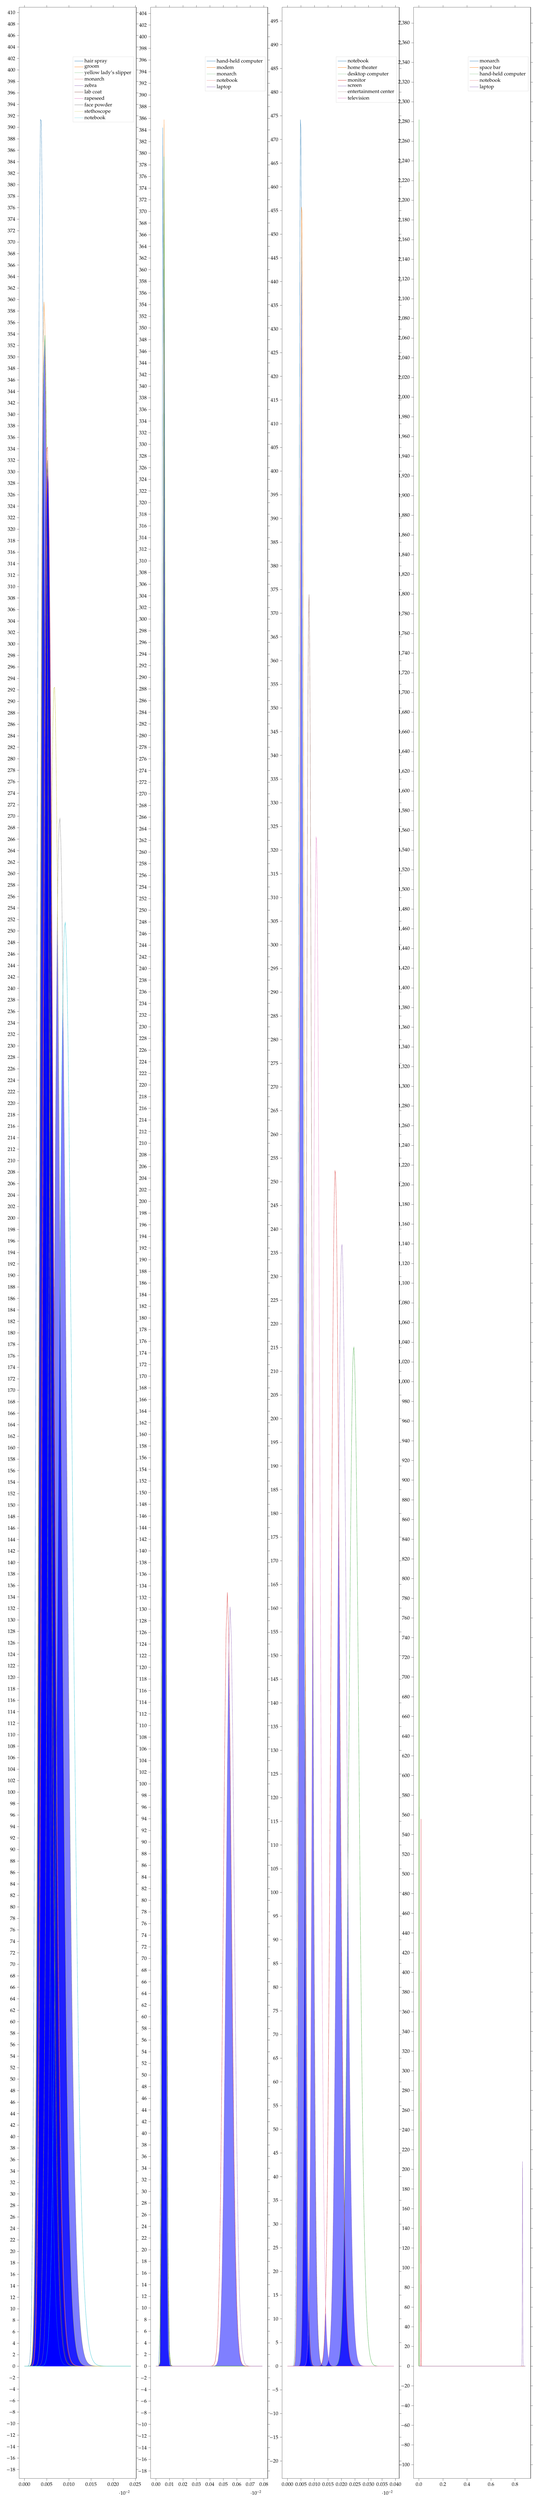
\begin{tikzpicture}

\definecolor{color0}{rgb}{0.12156862745098,0.466666666666667,0.705882352941177}
\definecolor{color1}{rgb}{1,0.498039215686275,0.0549019607843137}
\definecolor{color2}{rgb}{0.172549019607843,0.627450980392157,0.172549019607843}
\definecolor{color3}{rgb}{0.83921568627451,0.152941176470588,0.156862745098039}
\definecolor{color4}{rgb}{0.580392156862745,0.403921568627451,0.741176470588235}
\definecolor{color5}{rgb}{0.549019607843137,0.337254901960784,0.294117647058824}
\definecolor{color6}{rgb}{0.890196078431372,0.466666666666667,0.76078431372549}
\definecolor{color7}{rgb}{0.737254901960784,0.741176470588235,0.133333333333333}
\definecolor{color8}{rgb}{0.0901960784313725,0.745098039215686,0.811764705882353}

\begin{groupplot}[group style={group size=4 by 1}]
\nextgroupplot[
height=\figheight,
legend cell align={left},
legend style={fill opacity=0.8, draw opacity=1, text opacity=1, draw=white!80!black},
tick align=outside,
tick pos=both,
width=\figwidth,
x grid style={white!69.0196078431373!black},
xmin=-0.0012, xmax=0.0252,
xtick style={color=black},
xtick={-0.005,0,0.005,0.01,0.015,0.02,0.025,0.03},
xticklabels={−0.005,0.000,0.005,0.010,0.015,0.020,0.025,0.030},
y grid style={white!69.0196078431373!black},
ymin=-19.5670691114727, ymax=410.908451340926,
ytick style={color=black}
]
\path [draw=none, fill=blue, fill opacity=0.5]
(axis cs:0,0)
--(axis cs:0.0002,4.22795300245434e-13)
--(axis cs:0.0004,1.37496114174896e-08)
--(axis cs:0.0006,4.44349918357242e-06)
--(axis cs:0.0008,0.000217352763044482)
--(axis cs:0.001,0.00377803209216558)
--(axis cs:0.0012,0.0341292040287655)
--(axis cs:0.0014,0.196252804450894)
--(axis cs:0.0016,0.81078219972159)
--(axis cs:0.0018,2.60195337937075)
--(axis cs:0.002,6.84154460221035)
--(axis cs:0.0022,15.3102330091327)
--(axis cs:0.0024,29.989931796765)
--(axis cs:0.0026,52.5284673552818)
--(axis cs:0.0028,83.6444501303574)
--(axis cs:0.003,122.689795384513)
--(axis cs:0.0032,167.536087950985)
--(axis cs:0.0034,214.832099146605)
--(axis cs:0.0036,260.553774989619)
--(axis cs:0.0038,300.686244763745)
--(axis cs:0.004,331.861083501153)
--(axis cs:0.0042,350.659364364021)
--(axis cs:0.0044,316.671390945087)
--(axis cs:0.0046,278.132151246613)
--(axis cs:0.0048,238.141886324419)
--(axis cs:0.005,199.186771160928)
--(axis cs:0.0052,163.048755076709)
--(axis cs:0.0054,130.83056941505)
--(axis cs:0.0056,103.053206760269)
--(axis cs:0.0058,79.7873803369428)
--(axis cs:0.006,60.7897332615976)
--(axis cs:0.0062,45.6250166719352)
--(axis cs:0.0064,33.764694951832)
--(axis cs:0.0066,24.6593694570613)
--(axis cs:0.0068,17.7868661496403)
--(axis cs:0.007,12.6801601962024)
--(axis cs:0.0072,8.94007607834724)
--(axis cs:0.0074,6.23747618667221)
--(axis cs:0.0076,4.30890608686193)
--(axis cs:0.0078,2.94873796599512)
--(axis cs:0.008,1.99995481107366)
--(axis cs:0.0082,1.34495499920915)
--(axis cs:0.0084,0.897168396988933)
--(axis cs:0.0086,0.59385652774837)
--(axis cs:0.0088,0.390195217766181)
--(axis cs:0.009,0.254575414817491)
--(axis cs:0.0092,0.164974583259305)
--(axis cs:0.0094,0.106220200791715)
--(axis cs:0.0096,0.0679676620931031)
--(axis cs:0.0098,0.0432325808603513)
--(axis cs:0.01,0.0273423296596845)
--(axis cs:0.0102,0.0171977344356047)
--(axis cs:0.0104,0.0107599089132325)
--(axis cs:0.0106,0.00669780790315936)
--(axis cs:0.0108,0.00414881285588331)
--(axis cs:0.011,0.00255774928923221)
--(axis cs:0.0112,0.00156966462258963)
--(axis cs:0.0114,0.000959043980204529)
--(axis cs:0.0116,0.000583468440526314)
--(axis cs:0.0118,0.000353512309656768)
--(axis cs:0.012,0.000213333020725685)
--(axis cs:0.0122,0.000128242850643948)
--(axis cs:0.0124,7.68037201326851e-05)
--(axis cs:0.0126,4.58305761506692e-05)
--(axis cs:0.0128,2.72520977192749e-05)
--(axis cs:0.013,1.61495898117959e-05)
--(axis cs:0.0132,9.53857042332152e-06)
--(axis cs:0.0134,5.6157357557516e-06)
--(axis cs:0.0136,3.29587795741631e-06)
--(axis cs:0.0138,1.92847688063577e-06)
--(axis cs:0.014,1.12505239925148e-06)
--(axis cs:0.0142,6.54456317675556e-07)
--(axis cs:0.0144,3.79639444120029e-07)
--(axis cs:0.0146,2.19622342593566e-07)
--(axis cs:0.0148,1.26714616937668e-07)
--(axis cs:0.015,7.29207563822728e-08)
--(axis cs:0.0152,4.18579500369891e-08)
--(axis cs:0.0154,2.39681255123372e-08)
--(axis cs:0.0156,1.36913240004885e-08)
--(axis cs:0.0158,7.8025585154859e-09)
--(axis cs:0.016,4.43642182094435e-09)
--(axis cs:0.0162,2.51684199065801e-09)
--(axis cs:0.0164,1.4247171282791e-09)
--(axis cs:0.0166,8.04771081382379e-10)
--(axis cs:0.0168,4.53636274462889e-10)
--(axis cs:0.017,2.55184812810522e-10)
--(axis cs:0.0172,1.43262573263436e-10)
--(axis cs:0.0174,8.02712667488462e-11)
--(axis cs:0.0176,4.48905435239373e-11)
--(axis cs:0.0178,2.50573023493042e-11)
--(axis cs:0.018,1.3960957590044e-11)
--(axis cs:0.0182,7.76450428095243e-12)
--(axis cs:0.0184,4.31067763326576e-12)
--(axis cs:0.0186,2.3890530370788e-12)
--(axis cs:0.0188,1.32181029046682e-12)
--(axis cs:0.019,7.30112445413e-13)
--(axis cs:0.0192,4.02625619692298e-13)
--(axis cs:0.0194,2.21675354345489e-13)
--(axis cs:0.0196,1.21857053967287e-13)
--(axis cs:0.0198,6.68826864553411e-14)
--(axis cs:0.02,3.66537700284644e-14)
--(axis cs:0.0202,2.00575217613878e-14)
--(axis cs:0.0204,1.0959758809364e-14)
--(axis cs:0.0206,5.97999627347004e-15)
--(axis cs:0.0208,3.25827538993974e-15)
--(axis cs:0.021,1.77285035089687e-15)
--(axis cs:0.0212,9.63305278865802e-16)
--(axis cs:0.0214,5.22724971007102e-16)
--(axis cs:0.0216,2.83275877689995e-16)
--(axis cs:0.0218,1.53314174574747e-16)
--(axis cs:0.022,8.28705967052991e-17)
--(axis cs:0.0222,4.47376214030539e-17)
--(axis cs:0.0224,2.41217142550633e-17)
--(axis cs:0.0226,1.29901647606133e-17)
--(axis cs:0.0228,6.98715695218015e-18)
--(axis cs:0.023,3.75382142728391e-18)
--(axis cs:0.0232,2.01438141289907e-18)
--(axis cs:0.0234,1.07972288043767e-18)
--(axis cs:0.0236,5.78086370487335e-19)
--(axis cs:0.0238,3.09164855713053e-19)
--(axis cs:0.024,1.65162493477036e-19)
--cycle;
\path [draw=none, fill=blue, fill opacity=0.5]
(axis cs:0,0)
--(axis cs:0.0002,7.61192645735247e-14)
--(axis cs:0.0004,3.61092349697281e-09)
--(axis cs:0.0006,1.45540906761335e-06)
--(axis cs:0.0008,8.32729233244913e-05)
--(axis cs:0.001,0.00163463517706023)
--(axis cs:0.0012,0.016309637005717)
--(axis cs:0.0014,0.102008198661971)
--(axis cs:0.0016,0.453261075131758)
--(axis cs:0.0018,1.5511170267273)
--(axis cs:0.002,4.31978738912353)
--(axis cs:0.0022,10.1830168367104)
--(axis cs:0.0024,20.9167445288748)
--(axis cs:0.0026,38.2727217377937)
--(axis cs:0.0028,63.4606200393569)
--(axis cs:0.003,96.6581704221682)
--(axis cs:0.0032,136.725048683837)
--(axis cs:0.0034,181.227009291322)
--(axis cs:0.0036,226.769934038948)
--(axis cs:0.0038,269.547320550091)
--(axis cs:0.004,305.953317774446)
--(axis cs:0.0042,333.115658709357)
--(axis cs:0.0044,316.671390945087)
--(axis cs:0.0046,278.132151246613)
--(axis cs:0.0048,238.141886324419)
--(axis cs:0.005,199.186771160928)
--(axis cs:0.0052,163.048755076709)
--(axis cs:0.0054,130.83056941505)
--(axis cs:0.0056,103.053206760269)
--(axis cs:0.0058,79.7873803369428)
--(axis cs:0.006,60.7897332615976)
--(axis cs:0.0062,45.6250166719352)
--(axis cs:0.0064,33.764694951832)
--(axis cs:0.0066,24.6593694570613)
--(axis cs:0.0068,17.7868661496403)
--(axis cs:0.007,12.6801601962024)
--(axis cs:0.0072,8.94007607834724)
--(axis cs:0.0074,6.23747618667221)
--(axis cs:0.0076,4.30890608686193)
--(axis cs:0.0078,2.94873796599512)
--(axis cs:0.008,1.99995481107366)
--(axis cs:0.0082,1.34495499920915)
--(axis cs:0.0084,0.897168396988933)
--(axis cs:0.0086,0.59385652774837)
--(axis cs:0.0088,0.390195217766181)
--(axis cs:0.009,0.254575414817491)
--(axis cs:0.0092,0.164974583259305)
--(axis cs:0.0094,0.106220200791715)
--(axis cs:0.0096,0.0679676620931031)
--(axis cs:0.0098,0.0432325808603513)
--(axis cs:0.01,0.0273423296596845)
--(axis cs:0.0102,0.0171977344356047)
--(axis cs:0.0104,0.0107599089132325)
--(axis cs:0.0106,0.00669780790315936)
--(axis cs:0.0108,0.00414881285588331)
--(axis cs:0.011,0.00255774928923221)
--(axis cs:0.0112,0.00156966462258963)
--(axis cs:0.0114,0.000959043980204529)
--(axis cs:0.0116,0.000583468440526314)
--(axis cs:0.0118,0.000353512309656768)
--(axis cs:0.012,0.000213333020725685)
--(axis cs:0.0122,0.000128242850643948)
--(axis cs:0.0124,7.68037201326851e-05)
--(axis cs:0.0126,4.58305761506692e-05)
--(axis cs:0.0128,2.72520977192749e-05)
--(axis cs:0.013,1.61495898117959e-05)
--(axis cs:0.0132,9.53857042332152e-06)
--(axis cs:0.0134,5.6157357557516e-06)
--(axis cs:0.0136,3.29587795741631e-06)
--(axis cs:0.0138,1.92847688063577e-06)
--(axis cs:0.014,1.12505239925148e-06)
--(axis cs:0.0142,6.54456317675556e-07)
--(axis cs:0.0144,3.79639444120029e-07)
--(axis cs:0.0146,2.19622342593566e-07)
--(axis cs:0.0148,1.26714616937668e-07)
--(axis cs:0.015,7.29207563822728e-08)
--(axis cs:0.0152,4.18579500369891e-08)
--(axis cs:0.0154,2.39681255123372e-08)
--(axis cs:0.0156,1.36913240004885e-08)
--(axis cs:0.0158,7.8025585154859e-09)
--(axis cs:0.016,4.43642182094435e-09)
--(axis cs:0.0162,2.51684199065801e-09)
--(axis cs:0.0164,1.4247171282791e-09)
--(axis cs:0.0166,8.04771081382379e-10)
--(axis cs:0.0168,4.53636274462889e-10)
--(axis cs:0.017,2.55184812810522e-10)
--(axis cs:0.0172,1.43262573263436e-10)
--(axis cs:0.0174,8.02712667488462e-11)
--(axis cs:0.0176,4.48905435239373e-11)
--(axis cs:0.0178,2.50573023493042e-11)
--(axis cs:0.018,1.3960957590044e-11)
--(axis cs:0.0182,7.76450428095243e-12)
--(axis cs:0.0184,4.31067763326576e-12)
--(axis cs:0.0186,2.3890530370788e-12)
--(axis cs:0.0188,1.32181029046682e-12)
--(axis cs:0.019,7.30112445413e-13)
--(axis cs:0.0192,4.02625619692298e-13)
--(axis cs:0.0194,2.21675354345489e-13)
--(axis cs:0.0196,1.21857053967287e-13)
--(axis cs:0.0198,6.68826864553411e-14)
--(axis cs:0.02,3.66537700284644e-14)
--(axis cs:0.0202,2.00575217613878e-14)
--(axis cs:0.0204,1.0959758809364e-14)
--(axis cs:0.0206,5.97999627347004e-15)
--(axis cs:0.0208,3.25827538993974e-15)
--(axis cs:0.021,1.77285035089687e-15)
--(axis cs:0.0212,9.63305278865802e-16)
--(axis cs:0.0214,5.22724971007102e-16)
--(axis cs:0.0216,2.83275877689995e-16)
--(axis cs:0.0218,1.53314174574747e-16)
--(axis cs:0.022,8.28705967052991e-17)
--(axis cs:0.0222,4.47376214030539e-17)
--(axis cs:0.0224,2.41217142550633e-17)
--(axis cs:0.0226,1.29901647606133e-17)
--(axis cs:0.0228,6.98715695218015e-18)
--(axis cs:0.023,3.75382142728391e-18)
--(axis cs:0.0232,2.01438141289907e-18)
--(axis cs:0.0234,1.07972288043767e-18)
--(axis cs:0.0236,5.78086370487335e-19)
--(axis cs:0.0238,3.09164855713053e-19)
--(axis cs:0.024,1.65162493477036e-19)
--cycle;
\path [draw=none, fill=blue, fill opacity=0.5]
(axis cs:0,0)
--(axis cs:0.0002,1.63304653410572e-16)
--(axis cs:0.0004,2.90980802338031e-11)
--(axis cs:0.0006,2.54391471865381e-08)
--(axis cs:0.0008,2.52149359912999e-06)
--(axis cs:0.001,7.58076561312621e-05)
--(axis cs:0.0012,0.00107160766687709)
--(axis cs:0.0014,0.0089985803413974)
--(axis cs:0.0016,0.0516110463947514)
--(axis cs:0.0018,0.221227821059011)
--(axis cs:0.002,0.753634925751084)
--(axis cs:0.0022,2.13180511178777)
--(axis cs:0.0024,5.17199814367324)
--(axis cs:0.0026,11.0298671973361)
--(axis cs:0.0028,21.0757198851318)
--(axis cs:0.003,36.6331090584455)
--(axis cs:0.0032,58.6338009969209)
--(axis cs:0.0034,87.2857386482926)
--(axis cs:0.0036,121.857708878618)
--(axis cs:0.0038,160.652447408685)
--(axis cs:0.004,201.183753056193)
--(axis cs:0.0042,240.515622550635)
--(axis cs:0.0044,275.68210296399)
--(axis cs:0.0046,278.132151246613)
--(axis cs:0.0048,238.141886324419)
--(axis cs:0.005,199.186771160928)
--(axis cs:0.0052,163.048755076709)
--(axis cs:0.0054,130.83056941505)
--(axis cs:0.0056,103.053206760269)
--(axis cs:0.0058,79.7873803369428)
--(axis cs:0.006,60.7897332615976)
--(axis cs:0.0062,45.6250166719352)
--(axis cs:0.0064,33.764694951832)
--(axis cs:0.0066,24.6593694570613)
--(axis cs:0.0068,17.7868661496403)
--(axis cs:0.007,12.6801601962024)
--(axis cs:0.0072,8.94007607834724)
--(axis cs:0.0074,6.23747618667221)
--(axis cs:0.0076,4.30890608686193)
--(axis cs:0.0078,2.94873796599512)
--(axis cs:0.008,1.99995481107366)
--(axis cs:0.0082,1.34495499920915)
--(axis cs:0.0084,0.897168396988933)
--(axis cs:0.0086,0.59385652774837)
--(axis cs:0.0088,0.390195217766181)
--(axis cs:0.009,0.254575414817491)
--(axis cs:0.0092,0.164974583259305)
--(axis cs:0.0094,0.106220200791715)
--(axis cs:0.0096,0.0679676620931031)
--(axis cs:0.0098,0.0432325808603513)
--(axis cs:0.01,0.0273423296596845)
--(axis cs:0.0102,0.0171977344356047)
--(axis cs:0.0104,0.0107599089132325)
--(axis cs:0.0106,0.00669780790315936)
--(axis cs:0.0108,0.00414881285588331)
--(axis cs:0.011,0.00255774928923221)
--(axis cs:0.0112,0.00156966462258963)
--(axis cs:0.0114,0.000959043980204529)
--(axis cs:0.0116,0.000583468440526314)
--(axis cs:0.0118,0.000353512309656768)
--(axis cs:0.012,0.000213333020725685)
--(axis cs:0.0122,0.000128242850643948)
--(axis cs:0.0124,7.68037201326851e-05)
--(axis cs:0.0126,4.58305761506692e-05)
--(axis cs:0.0128,2.72520977192749e-05)
--(axis cs:0.013,1.61495898117959e-05)
--(axis cs:0.0132,9.53857042332152e-06)
--(axis cs:0.0134,5.6157357557516e-06)
--(axis cs:0.0136,3.29587795741631e-06)
--(axis cs:0.0138,1.92847688063577e-06)
--(axis cs:0.014,1.12505239925148e-06)
--(axis cs:0.0142,6.54456317675556e-07)
--(axis cs:0.0144,3.79639444120029e-07)
--(axis cs:0.0146,2.19622342593566e-07)
--(axis cs:0.0148,1.26714616937668e-07)
--(axis cs:0.015,7.29207563822728e-08)
--(axis cs:0.0152,4.18579500369891e-08)
--(axis cs:0.0154,2.39681255123372e-08)
--(axis cs:0.0156,1.36913240004885e-08)
--(axis cs:0.0158,7.8025585154859e-09)
--(axis cs:0.016,4.43642182094435e-09)
--(axis cs:0.0162,2.51684199065801e-09)
--(axis cs:0.0164,1.4247171282791e-09)
--(axis cs:0.0166,8.04771081382379e-10)
--(axis cs:0.0168,4.53636274462889e-10)
--(axis cs:0.017,2.55184812810522e-10)
--(axis cs:0.0172,1.43262573263436e-10)
--(axis cs:0.0174,8.02712667488462e-11)
--(axis cs:0.0176,4.48905435239373e-11)
--(axis cs:0.0178,2.50573023493042e-11)
--(axis cs:0.018,1.3960957590044e-11)
--(axis cs:0.0182,7.76450428095243e-12)
--(axis cs:0.0184,4.31067763326576e-12)
--(axis cs:0.0186,2.3890530370788e-12)
--(axis cs:0.0188,1.32181029046682e-12)
--(axis cs:0.019,7.30112445413e-13)
--(axis cs:0.0192,4.02625619692298e-13)
--(axis cs:0.0194,2.21675354345489e-13)
--(axis cs:0.0196,1.21857053967287e-13)
--(axis cs:0.0198,6.68826864553411e-14)
--(axis cs:0.02,3.66537700284644e-14)
--(axis cs:0.0202,2.00575217613878e-14)
--(axis cs:0.0204,1.0959758809364e-14)
--(axis cs:0.0206,5.97999627347004e-15)
--(axis cs:0.0208,3.25827538993974e-15)
--(axis cs:0.021,1.77285035089687e-15)
--(axis cs:0.0212,9.63305278865802e-16)
--(axis cs:0.0214,5.22724971007102e-16)
--(axis cs:0.0216,2.83275877689995e-16)
--(axis cs:0.0218,1.53314174574747e-16)
--(axis cs:0.022,8.28705967052991e-17)
--(axis cs:0.0222,4.47376214030539e-17)
--(axis cs:0.0224,2.41217142550633e-17)
--(axis cs:0.0226,1.29901647606133e-17)
--(axis cs:0.0228,6.98715695218015e-18)
--(axis cs:0.023,3.75382142728391e-18)
--(axis cs:0.0232,2.01438141289907e-18)
--(axis cs:0.0234,1.07972288043767e-18)
--(axis cs:0.0236,5.78086370487335e-19)
--(axis cs:0.0238,3.09164855713053e-19)
--(axis cs:0.024,1.65162493477036e-19)
--cycle;
\path [draw=none, fill=blue, fill opacity=0.5]
(axis cs:0,0)
--(axis cs:0.0002,2.87061962533969e-17)
--(axis cs:0.0004,7.38215500264892e-12)
--(axis cs:0.0006,7.99925233557908e-09)
--(axis cs:0.0008,9.23345890210269e-07)
--(axis cs:0.001,3.12426163997331e-05)
--(axis cs:0.0012,0.000486425585682615)
--(axis cs:0.0014,0.00443227584242255)
--(axis cs:0.0016,0.0272853176447845)
--(axis cs:0.0018,0.124491716808887)
--(axis cs:0.002,0.448457426929982)
--(axis cs:0.0022,1.33431227744341)
--(axis cs:0.0024,3.39008775333182)
--(axis cs:0.0026,7.54334486722043)
--(axis cs:0.0028,14.9917839314935)
--(axis cs:0.003,27.0300203986886)
--(axis cs:0.0032,44.7711936223266)
--(axis cs:0.0034,68.829161876082)
--(axis cs:0.0036,99.0522136164206)
--(axis cs:0.0038,134.390978721141)
--(axis cs:0.004,172.945707968733)
--(axis cs:0.0042,212.187129650739)
--(axis cs:0.0044,249.299540863043)
--(axis cs:0.0046,278.132151246613)
--(axis cs:0.0048,238.141886324419)
--(axis cs:0.005,199.186771160928)
--(axis cs:0.0052,163.048755076709)
--(axis cs:0.0054,130.83056941505)
--(axis cs:0.0056,103.053206760269)
--(axis cs:0.0058,79.7873803369428)
--(axis cs:0.006,60.7897332615976)
--(axis cs:0.0062,45.6250166719352)
--(axis cs:0.0064,33.764694951832)
--(axis cs:0.0066,24.6593694570613)
--(axis cs:0.0068,17.7868661496403)
--(axis cs:0.007,12.6801601962024)
--(axis cs:0.0072,8.94007607834724)
--(axis cs:0.0074,6.23747618667221)
--(axis cs:0.0076,4.30890608686193)
--(axis cs:0.0078,2.94873796599512)
--(axis cs:0.008,1.99995481107366)
--(axis cs:0.0082,1.34495499920915)
--(axis cs:0.0084,0.897168396988933)
--(axis cs:0.0086,0.59385652774837)
--(axis cs:0.0088,0.390195217766181)
--(axis cs:0.009,0.254575414817491)
--(axis cs:0.0092,0.164974583259305)
--(axis cs:0.0094,0.106220200791715)
--(axis cs:0.0096,0.0679676620931031)
--(axis cs:0.0098,0.0432325808603513)
--(axis cs:0.01,0.0273423296596845)
--(axis cs:0.0102,0.0171977344356047)
--(axis cs:0.0104,0.0107599089132325)
--(axis cs:0.0106,0.00669780790315936)
--(axis cs:0.0108,0.00414881285588331)
--(axis cs:0.011,0.00255774928923221)
--(axis cs:0.0112,0.00156966462258963)
--(axis cs:0.0114,0.000959043980204529)
--(axis cs:0.0116,0.000583468440526314)
--(axis cs:0.0118,0.000353512309656768)
--(axis cs:0.012,0.000213333020725685)
--(axis cs:0.0122,0.000128242850643948)
--(axis cs:0.0124,7.68037201326851e-05)
--(axis cs:0.0126,4.58305761506692e-05)
--(axis cs:0.0128,2.72520977192749e-05)
--(axis cs:0.013,1.61495898117959e-05)
--(axis cs:0.0132,9.53857042332152e-06)
--(axis cs:0.0134,5.6157357557516e-06)
--(axis cs:0.0136,3.29587795741631e-06)
--(axis cs:0.0138,1.92847688063577e-06)
--(axis cs:0.014,1.12505239925148e-06)
--(axis cs:0.0142,6.54456317675556e-07)
--(axis cs:0.0144,3.79639444120029e-07)
--(axis cs:0.0146,2.19622342593566e-07)
--(axis cs:0.0148,1.26714616937668e-07)
--(axis cs:0.015,7.29207563822728e-08)
--(axis cs:0.0152,4.18579500369891e-08)
--(axis cs:0.0154,2.39681255123372e-08)
--(axis cs:0.0156,1.36913240004885e-08)
--(axis cs:0.0158,7.8025585154859e-09)
--(axis cs:0.016,4.43642182094435e-09)
--(axis cs:0.0162,2.51684199065801e-09)
--(axis cs:0.0164,1.4247171282791e-09)
--(axis cs:0.0166,8.04771081382379e-10)
--(axis cs:0.0168,4.53636274462889e-10)
--(axis cs:0.017,2.55184812810522e-10)
--(axis cs:0.0172,1.43262573263436e-10)
--(axis cs:0.0174,8.02712667488462e-11)
--(axis cs:0.0176,4.48905435239373e-11)
--(axis cs:0.0178,2.50573023493042e-11)
--(axis cs:0.018,1.3960957590044e-11)
--(axis cs:0.0182,7.76450428095243e-12)
--(axis cs:0.0184,4.31067763326576e-12)
--(axis cs:0.0186,2.3890530370788e-12)
--(axis cs:0.0188,1.32181029046682e-12)
--(axis cs:0.019,7.30112445413e-13)
--(axis cs:0.0192,4.02625619692298e-13)
--(axis cs:0.0194,2.21675354345489e-13)
--(axis cs:0.0196,1.21857053967287e-13)
--(axis cs:0.0198,6.68826864553411e-14)
--(axis cs:0.02,3.66537700284644e-14)
--(axis cs:0.0202,2.00575217613878e-14)
--(axis cs:0.0204,1.0959758809364e-14)
--(axis cs:0.0206,5.97999627347004e-15)
--(axis cs:0.0208,3.25827538993974e-15)
--(axis cs:0.021,1.77285035089687e-15)
--(axis cs:0.0212,9.63305278865802e-16)
--(axis cs:0.0214,5.22724971007102e-16)
--(axis cs:0.0216,2.83275877689995e-16)
--(axis cs:0.0218,1.53314174574747e-16)
--(axis cs:0.022,8.28705967052991e-17)
--(axis cs:0.0222,4.47376214030539e-17)
--(axis cs:0.0224,2.41217142550633e-17)
--(axis cs:0.0226,1.29901647606133e-17)
--(axis cs:0.0228,6.98715695218015e-18)
--(axis cs:0.023,3.75382142728391e-18)
--(axis cs:0.0232,2.01438141289907e-18)
--(axis cs:0.0234,1.07972288043767e-18)
--(axis cs:0.0236,5.78086370487335e-19)
--(axis cs:0.0238,3.09164855713053e-19)
--(axis cs:0.024,1.65162493477036e-19)
--cycle;
\path [draw=none, fill=blue, fill opacity=0.5]
(axis cs:0,0)
--(axis cs:0.0002,4.77632767978611e-17)
--(axis cs:0.0004,1.10350468092225e-11)
--(axis cs:0.0006,1.12309897522798e-08)
--(axis cs:0.0008,1.23997965836469e-06)
--(axis cs:0.001,4.05331104838323e-05)
--(axis cs:0.0012,0.000613522820835944)
--(axis cs:0.0014,0.00545862533187201)
--(axis cs:0.0016,0.032916327874361)
--(axis cs:0.0018,0.147470611530503)
--(axis cs:0.002,0.522639852402313)
--(axis cs:0.0022,1.53224950990862)
--(axis cs:0.0024,3.84087832479369)
--(axis cs:0.0026,8.44109535473997)
--(axis cs:0.0028,16.5844717211536)
--(axis cs:0.003,29.5836281445369)
--(axis cs:0.0032,48.5131391024827)
--(axis cs:0.0034,73.884182008032)
--(axis cs:0.0036,105.388702355709)
--(axis cs:0.0038,141.794147211553)
--(axis cs:0.004,181.026617480686)
--(axis cs:0.0042,220.426658502137)
--(axis cs:0.0044,257.117315904375)
--(axis cs:0.0046,278.132151246613)
--(axis cs:0.0048,238.141886324419)
--(axis cs:0.005,199.186771160928)
--(axis cs:0.0052,163.048755076709)
--(axis cs:0.0054,130.83056941505)
--(axis cs:0.0056,103.053206760269)
--(axis cs:0.0058,79.7873803369428)
--(axis cs:0.006,60.7897332615976)
--(axis cs:0.0062,45.6250166719352)
--(axis cs:0.0064,33.764694951832)
--(axis cs:0.0066,24.6593694570613)
--(axis cs:0.0068,17.7868661496403)
--(axis cs:0.007,12.6801601962024)
--(axis cs:0.0072,8.94007607834724)
--(axis cs:0.0074,6.23747618667221)
--(axis cs:0.0076,4.30890608686193)
--(axis cs:0.0078,2.94873796599512)
--(axis cs:0.008,1.99995481107366)
--(axis cs:0.0082,1.34495499920915)
--(axis cs:0.0084,0.897168396988933)
--(axis cs:0.0086,0.59385652774837)
--(axis cs:0.0088,0.390195217766181)
--(axis cs:0.009,0.254575414817491)
--(axis cs:0.0092,0.164974583259305)
--(axis cs:0.0094,0.106220200791715)
--(axis cs:0.0096,0.0679676620931031)
--(axis cs:0.0098,0.0432325808603513)
--(axis cs:0.01,0.0273423296596845)
--(axis cs:0.0102,0.0171977344356047)
--(axis cs:0.0104,0.0107599089132325)
--(axis cs:0.0106,0.00669780790315936)
--(axis cs:0.0108,0.00414881285588331)
--(axis cs:0.011,0.00255774928923221)
--(axis cs:0.0112,0.00156966462258963)
--(axis cs:0.0114,0.000959043980204529)
--(axis cs:0.0116,0.000583468440526314)
--(axis cs:0.0118,0.000353512309656768)
--(axis cs:0.012,0.000213333020725685)
--(axis cs:0.0122,0.000128242850643948)
--(axis cs:0.0124,7.68037201326851e-05)
--(axis cs:0.0126,4.58305761506692e-05)
--(axis cs:0.0128,2.72520977192749e-05)
--(axis cs:0.013,1.61495898117959e-05)
--(axis cs:0.0132,9.53857042332152e-06)
--(axis cs:0.0134,5.6157357557516e-06)
--(axis cs:0.0136,3.29587795741631e-06)
--(axis cs:0.0138,1.92847688063577e-06)
--(axis cs:0.014,1.12505239925148e-06)
--(axis cs:0.0142,6.54456317675556e-07)
--(axis cs:0.0144,3.79639444120029e-07)
--(axis cs:0.0146,2.19622342593566e-07)
--(axis cs:0.0148,1.26714616937668e-07)
--(axis cs:0.015,7.29207563822728e-08)
--(axis cs:0.0152,4.18579500369891e-08)
--(axis cs:0.0154,2.39681255123372e-08)
--(axis cs:0.0156,1.36913240004885e-08)
--(axis cs:0.0158,7.8025585154859e-09)
--(axis cs:0.016,4.43642182094435e-09)
--(axis cs:0.0162,2.51684199065801e-09)
--(axis cs:0.0164,1.4247171282791e-09)
--(axis cs:0.0166,8.04771081382379e-10)
--(axis cs:0.0168,4.53636274462889e-10)
--(axis cs:0.017,2.55184812810522e-10)
--(axis cs:0.0172,1.43262573263436e-10)
--(axis cs:0.0174,8.02712667488462e-11)
--(axis cs:0.0176,4.48905435239373e-11)
--(axis cs:0.0178,2.50573023493042e-11)
--(axis cs:0.018,1.3960957590044e-11)
--(axis cs:0.0182,7.76450428095243e-12)
--(axis cs:0.0184,4.31067763326576e-12)
--(axis cs:0.0186,2.3890530370788e-12)
--(axis cs:0.0188,1.32181029046682e-12)
--(axis cs:0.019,7.30112445413e-13)
--(axis cs:0.0192,4.02625619692298e-13)
--(axis cs:0.0194,2.21675354345489e-13)
--(axis cs:0.0196,1.21857053967287e-13)
--(axis cs:0.0198,6.68826864553411e-14)
--(axis cs:0.02,3.66537700284644e-14)
--(axis cs:0.0202,2.00575217613878e-14)
--(axis cs:0.0204,1.0959758809364e-14)
--(axis cs:0.0206,5.97999627347004e-15)
--(axis cs:0.0208,3.25827538993974e-15)
--(axis cs:0.021,1.77285035089687e-15)
--(axis cs:0.0212,9.63305278865802e-16)
--(axis cs:0.0214,5.22724971007102e-16)
--(axis cs:0.0216,2.83275877689995e-16)
--(axis cs:0.0218,1.53314174574747e-16)
--(axis cs:0.022,8.28705967052991e-17)
--(axis cs:0.0222,4.47376214030539e-17)
--(axis cs:0.0224,2.41217142550633e-17)
--(axis cs:0.0226,1.29901647606133e-17)
--(axis cs:0.0228,6.98715695218015e-18)
--(axis cs:0.023,3.75382142728391e-18)
--(axis cs:0.0232,2.01438141289907e-18)
--(axis cs:0.0234,1.07972288043767e-18)
--(axis cs:0.0236,5.78086370487335e-19)
--(axis cs:0.0238,3.09164855713053e-19)
--(axis cs:0.024,1.65162493477036e-19)
--cycle;
\path [draw=none, fill=blue, fill opacity=0.5]
(axis cs:0,0)
--(axis cs:0.0002,2.50033281924293e-17)
--(axis cs:0.0004,6.61920264526063e-12)
--(axis cs:0.0006,7.29531684613714e-09)
--(axis cs:0.0008,8.52296949347681e-07)
--(axis cs:0.001,2.91093689969302e-05)
--(axis cs:0.0012,0.000456687181093467)
--(axis cs:0.0014,0.00418826597701668)
--(axis cs:0.0016,0.025927869467974)
--(axis cs:0.0018,0.118883729553988)
--(axis cs:0.002,0.43015163399355)
--(axis cs:0.0022,1.28497176113775)
--(axis cs:0.0024,3.27666446986953)
--(axis cs:0.0026,7.31548767742108)
--(axis cs:0.0028,14.5842153965101)
--(axis cs:0.003,26.3714255968948)
--(axis cs:0.0032,43.7988227032249)
--(axis cs:0.0034,67.5058869162191)
--(axis cs:0.0036,97.3813437364043)
--(axis cs:0.0038,132.424374144004)
--(axis cs:0.004,170.782523087049)
--(axis cs:0.0042,209.96311643966)
--(axis cs:0.0044,247.169302110898)
--(axis cs:0.0046,278.132151246613)
--(axis cs:0.0048,238.141886324419)
--(axis cs:0.005,199.186771160928)
--(axis cs:0.0052,163.048755076709)
--(axis cs:0.0054,130.83056941505)
--(axis cs:0.0056,103.053206760269)
--(axis cs:0.0058,79.7873803369428)
--(axis cs:0.006,60.7897332615976)
--(axis cs:0.0062,45.6250166719352)
--(axis cs:0.0064,33.764694951832)
--(axis cs:0.0066,24.6593694570613)
--(axis cs:0.0068,17.7868661496403)
--(axis cs:0.007,12.6801601962024)
--(axis cs:0.0072,8.94007607834724)
--(axis cs:0.0074,6.23747618667221)
--(axis cs:0.0076,4.30890608686193)
--(axis cs:0.0078,2.94873796599512)
--(axis cs:0.008,1.99995481107366)
--(axis cs:0.0082,1.34495499920915)
--(axis cs:0.0084,0.897168396988933)
--(axis cs:0.0086,0.59385652774837)
--(axis cs:0.0088,0.390195217766181)
--(axis cs:0.009,0.254575414817491)
--(axis cs:0.0092,0.164974583259305)
--(axis cs:0.0094,0.106220200791715)
--(axis cs:0.0096,0.0679676620931031)
--(axis cs:0.0098,0.0432325808603513)
--(axis cs:0.01,0.0273423296596845)
--(axis cs:0.0102,0.0171977344356047)
--(axis cs:0.0104,0.0107599089132325)
--(axis cs:0.0106,0.00669780790315936)
--(axis cs:0.0108,0.00414881285588331)
--(axis cs:0.011,0.00255774928923221)
--(axis cs:0.0112,0.00156966462258963)
--(axis cs:0.0114,0.000959043980204529)
--(axis cs:0.0116,0.000583468440526314)
--(axis cs:0.0118,0.000353512309656768)
--(axis cs:0.012,0.000213333020725685)
--(axis cs:0.0122,0.000128242850643948)
--(axis cs:0.0124,7.68037201326851e-05)
--(axis cs:0.0126,4.58305761506692e-05)
--(axis cs:0.0128,2.72520977192749e-05)
--(axis cs:0.013,1.61495898117959e-05)
--(axis cs:0.0132,9.53857042332152e-06)
--(axis cs:0.0134,5.6157357557516e-06)
--(axis cs:0.0136,3.29587795741631e-06)
--(axis cs:0.0138,1.92847688063577e-06)
--(axis cs:0.014,1.12505239925148e-06)
--(axis cs:0.0142,6.54456317675556e-07)
--(axis cs:0.0144,3.79639444120029e-07)
--(axis cs:0.0146,2.19622342593566e-07)
--(axis cs:0.0148,1.26714616937668e-07)
--(axis cs:0.015,7.29207563822728e-08)
--(axis cs:0.0152,4.18579500369891e-08)
--(axis cs:0.0154,2.39681255123372e-08)
--(axis cs:0.0156,1.36913240004885e-08)
--(axis cs:0.0158,7.8025585154859e-09)
--(axis cs:0.016,4.43642182094435e-09)
--(axis cs:0.0162,2.51684199065801e-09)
--(axis cs:0.0164,1.4247171282791e-09)
--(axis cs:0.0166,8.04771081382379e-10)
--(axis cs:0.0168,4.53636274462889e-10)
--(axis cs:0.017,2.55184812810522e-10)
--(axis cs:0.0172,1.43262573263436e-10)
--(axis cs:0.0174,8.02712667488462e-11)
--(axis cs:0.0176,4.48905435239373e-11)
--(axis cs:0.0178,2.50573023493042e-11)
--(axis cs:0.018,1.3960957590044e-11)
--(axis cs:0.0182,7.76450428095243e-12)
--(axis cs:0.0184,4.31067763326576e-12)
--(axis cs:0.0186,2.3890530370788e-12)
--(axis cs:0.0188,1.32181029046682e-12)
--(axis cs:0.019,7.30112445413e-13)
--(axis cs:0.0192,4.02625619692298e-13)
--(axis cs:0.0194,2.21675354345489e-13)
--(axis cs:0.0196,1.21857053967287e-13)
--(axis cs:0.0198,6.68826864553411e-14)
--(axis cs:0.02,3.66537700284644e-14)
--(axis cs:0.0202,2.00575217613878e-14)
--(axis cs:0.0204,1.0959758809364e-14)
--(axis cs:0.0206,5.97999627347004e-15)
--(axis cs:0.0208,3.25827538993974e-15)
--(axis cs:0.021,1.77285035089687e-15)
--(axis cs:0.0212,9.63305278865802e-16)
--(axis cs:0.0214,5.22724971007102e-16)
--(axis cs:0.0216,2.83275877689995e-16)
--(axis cs:0.0218,1.53314174574747e-16)
--(axis cs:0.022,8.28705967052991e-17)
--(axis cs:0.0222,4.47376214030539e-17)
--(axis cs:0.0224,2.41217142550633e-17)
--(axis cs:0.0226,1.29901647606133e-17)
--(axis cs:0.0228,6.98715695218015e-18)
--(axis cs:0.023,3.75382142728391e-18)
--(axis cs:0.0232,2.01438141289907e-18)
--(axis cs:0.0234,1.07972288043767e-18)
--(axis cs:0.0236,5.78086370487335e-19)
--(axis cs:0.0238,3.09164855713053e-19)
--(axis cs:0.024,1.65162493477036e-19)
--cycle;
\path [draw=none, fill=blue, fill opacity=0.5]
(axis cs:0,0)
--(axis cs:0.0002,4.38630231113233e-32)
--(axis cs:0.0004,9.42164546775413e-24)
--(axis cs:0.0006,5.22996289695702e-19)
--(axis cs:0.0008,9.86216555458081e-16)
--(axis cs:0.001,2.9143627354464e-13)
--(axis cs:0.0012,2.66669889722348e-11)
--(axis cs:0.0014,1.08650456690335e-09)
--(axis cs:0.0016,2.44844210199571e-08)
--(axis cs:0.0018,3.50988320156314e-07)
--(axis cs:0.002,3.52140105748224e-06)
--(axis cs:0.0022,2.64692151139118e-05)
--(axis cs:0.0024,0.000156751672867648)
--(axis cs:0.0026,0.000759830128964595)
--(axis cs:0.0028,0.00310561691820713)
--(axis cs:0.003,0.0109579090659142)
--(axis cs:0.0032,0.034016993111393)
--(axis cs:0.0034,0.0943609589409247)
--(axis cs:0.0036,0.236919036551997)
--(axis cs:0.0038,0.544246235965627)
--(axis cs:0.004,1.15434405660579)
--(axis cs:0.0042,2.27822422319553)
--(axis cs:0.0044,4.21196189035521)
--(axis cs:0.0046,7.33697307600828)
--(axis cs:0.0048,12.1029173241866)
--(axis cs:0.005,18.9902597620454)
--(axis cs:0.0052,28.4537592035236)
--(axis cs:0.0054,40.8529986597383)
--(axis cs:0.0056,56.3802313963309)
--(axis cs:0.0058,74.9980614577203)
--(axis cs:0.006,60.7897332615976)
--(axis cs:0.0062,45.6250166719352)
--(axis cs:0.0064,33.764694951832)
--(axis cs:0.0066,24.6593694570613)
--(axis cs:0.0068,17.7868661496403)
--(axis cs:0.007,12.6801601962024)
--(axis cs:0.0072,8.94007607834724)
--(axis cs:0.0074,6.23747618667221)
--(axis cs:0.0076,4.30890608686193)
--(axis cs:0.0078,2.94873796599512)
--(axis cs:0.008,1.99995481107366)
--(axis cs:0.0082,1.34495499920915)
--(axis cs:0.0084,0.897168396988933)
--(axis cs:0.0086,0.59385652774837)
--(axis cs:0.0088,0.390195217766181)
--(axis cs:0.009,0.254575414817491)
--(axis cs:0.0092,0.164974583259305)
--(axis cs:0.0094,0.106220200791715)
--(axis cs:0.0096,0.0679676620931031)
--(axis cs:0.0098,0.0432325808603513)
--(axis cs:0.01,0.0273423296596845)
--(axis cs:0.0102,0.0171977344356047)
--(axis cs:0.0104,0.0107599089132325)
--(axis cs:0.0106,0.00669780790315936)
--(axis cs:0.0108,0.00414881285588331)
--(axis cs:0.011,0.00255774928923221)
--(axis cs:0.0112,0.00156966462258963)
--(axis cs:0.0114,0.000959043980204529)
--(axis cs:0.0116,0.000583468440526314)
--(axis cs:0.0118,0.000353512309656768)
--(axis cs:0.012,0.000213333020725685)
--(axis cs:0.0122,0.000128242850643948)
--(axis cs:0.0124,7.68037201326851e-05)
--(axis cs:0.0126,4.58305761506692e-05)
--(axis cs:0.0128,2.72520977192749e-05)
--(axis cs:0.013,1.61495898117959e-05)
--(axis cs:0.0132,9.53857042332152e-06)
--(axis cs:0.0134,5.6157357557516e-06)
--(axis cs:0.0136,3.29587795741631e-06)
--(axis cs:0.0138,1.92847688063577e-06)
--(axis cs:0.014,1.12505239925148e-06)
--(axis cs:0.0142,6.54456317675556e-07)
--(axis cs:0.0144,3.79639444120029e-07)
--(axis cs:0.0146,2.19622342593566e-07)
--(axis cs:0.0148,1.26714616937668e-07)
--(axis cs:0.015,7.29207563822728e-08)
--(axis cs:0.0152,4.18579500369891e-08)
--(axis cs:0.0154,2.39681255123372e-08)
--(axis cs:0.0156,1.36913240004885e-08)
--(axis cs:0.0158,7.8025585154859e-09)
--(axis cs:0.016,4.43642182094435e-09)
--(axis cs:0.0162,2.51684199065801e-09)
--(axis cs:0.0164,1.4247171282791e-09)
--(axis cs:0.0166,8.04771081382379e-10)
--(axis cs:0.0168,4.53636274462889e-10)
--(axis cs:0.017,2.55184812810522e-10)
--(axis cs:0.0172,1.43262573263436e-10)
--(axis cs:0.0174,8.02712667488462e-11)
--(axis cs:0.0176,4.48905435239373e-11)
--(axis cs:0.0178,2.50573023493042e-11)
--(axis cs:0.018,1.3960957590044e-11)
--(axis cs:0.0182,7.76450428095243e-12)
--(axis cs:0.0184,4.31067763326576e-12)
--(axis cs:0.0186,2.3890530370788e-12)
--(axis cs:0.0188,1.32181029046682e-12)
--(axis cs:0.019,7.30112445413e-13)
--(axis cs:0.0192,4.02625619692298e-13)
--(axis cs:0.0194,2.21675354345489e-13)
--(axis cs:0.0196,1.21857053967287e-13)
--(axis cs:0.0198,6.68826864553411e-14)
--(axis cs:0.02,3.66537700284644e-14)
--(axis cs:0.0202,2.00575217613878e-14)
--(axis cs:0.0204,1.0959758809364e-14)
--(axis cs:0.0206,5.97999627347004e-15)
--(axis cs:0.0208,3.25827538993974e-15)
--(axis cs:0.021,1.77285035089687e-15)
--(axis cs:0.0212,9.63305278865802e-16)
--(axis cs:0.0214,5.22724971007102e-16)
--(axis cs:0.0216,2.83275877689995e-16)
--(axis cs:0.0218,1.53314174574747e-16)
--(axis cs:0.022,8.28705967052991e-17)
--(axis cs:0.0222,4.47376214030539e-17)
--(axis cs:0.0224,2.41217142550633e-17)
--(axis cs:0.0226,1.29901647606133e-17)
--(axis cs:0.0228,6.98715695218015e-18)
--(axis cs:0.023,3.75382142728391e-18)
--(axis cs:0.0232,2.01438141289907e-18)
--(axis cs:0.0234,1.07972288043767e-18)
--(axis cs:0.0236,5.78086370487335e-19)
--(axis cs:0.0238,3.09164855713053e-19)
--(axis cs:0.024,1.65162493477036e-19)
--cycle;
\path [draw=none, fill=blue, fill opacity=0.5]
(axis cs:0,0)
--(axis cs:0.0002,4.28964223063707e-25)
--(axis cs:0.0004,4.23925669893049e-18)
--(axis cs:0.0006,3.8843035174309e-14)
--(axis cs:0.0008,2.03980960361959e-11)
--(axis cs:0.001,2.23578413477403e-09)
--(axis cs:0.0012,9.09612932925116e-08)
--(axis cs:0.0014,1.86740983355346e-06)
--(axis cs:0.0016,2.32374652780952e-05)
--(axis cs:0.0018,0.00019726676995222)
--(axis cs:0.002,0.00123850159771812)
--(axis cs:0.0022,0.00609150384571705)
--(axis cs:0.0024,0.0244907822733581)
--(axis cs:0.0026,0.0831291604329364)
--(axis cs:0.0028,0.244273624310176)
--(axis cs:0.003,0.633888506344497)
--(axis cs:0.0032,1.47614150045633)
--(axis cs:0.0034,3.12549923236712)
--(axis cs:0.0036,6.08284419664121)
--(axis cs:0.0038,10.9810360144135)
--(axis cs:0.004,18.5299350809066)
--(axis cs:0.0042,29.4207126030825)
--(axis cs:0.0044,44.2015281358291)
--(axis cs:0.0046,63.1472686753469)
--(axis cs:0.0048,86.1512421387252)
--(axis cs:0.005,112.664536610035)
--(axis cs:0.0052,141.699695822165)
--(axis cs:0.0054,130.83056941505)
--(axis cs:0.0056,103.053206760269)
--(axis cs:0.0058,79.7873803369428)
--(axis cs:0.006,60.7897332615976)
--(axis cs:0.0062,45.6250166719352)
--(axis cs:0.0064,33.764694951832)
--(axis cs:0.0066,24.6593694570613)
--(axis cs:0.0068,17.7868661496403)
--(axis cs:0.007,12.6801601962024)
--(axis cs:0.0072,8.94007607834724)
--(axis cs:0.0074,6.23747618667221)
--(axis cs:0.0076,4.30890608686193)
--(axis cs:0.0078,2.94873796599512)
--(axis cs:0.008,1.99995481107366)
--(axis cs:0.0082,1.34495499920915)
--(axis cs:0.0084,0.897168396988933)
--(axis cs:0.0086,0.59385652774837)
--(axis cs:0.0088,0.390195217766181)
--(axis cs:0.009,0.254575414817491)
--(axis cs:0.0092,0.164974583259305)
--(axis cs:0.0094,0.106220200791715)
--(axis cs:0.0096,0.0679676620931031)
--(axis cs:0.0098,0.0432325808603513)
--(axis cs:0.01,0.0273423296596845)
--(axis cs:0.0102,0.0171977344356047)
--(axis cs:0.0104,0.0107599089132325)
--(axis cs:0.0106,0.00669780790315936)
--(axis cs:0.0108,0.00414881285588331)
--(axis cs:0.011,0.00255774928923221)
--(axis cs:0.0112,0.00156966462258963)
--(axis cs:0.0114,0.000959043980204529)
--(axis cs:0.0116,0.000583468440526314)
--(axis cs:0.0118,0.000353512309656768)
--(axis cs:0.012,0.000213333020725685)
--(axis cs:0.0122,0.000128242850643948)
--(axis cs:0.0124,7.68037201326851e-05)
--(axis cs:0.0126,4.58305761506692e-05)
--(axis cs:0.0128,2.72520977192749e-05)
--(axis cs:0.013,1.61495898117959e-05)
--(axis cs:0.0132,9.53857042332152e-06)
--(axis cs:0.0134,5.6157357557516e-06)
--(axis cs:0.0136,3.29587795741631e-06)
--(axis cs:0.0138,1.92847688063577e-06)
--(axis cs:0.014,1.12505239925148e-06)
--(axis cs:0.0142,6.54456317675556e-07)
--(axis cs:0.0144,3.79639444120029e-07)
--(axis cs:0.0146,2.19622342593566e-07)
--(axis cs:0.0148,1.26714616937668e-07)
--(axis cs:0.015,7.29207563822728e-08)
--(axis cs:0.0152,4.18579500369891e-08)
--(axis cs:0.0154,2.39681255123372e-08)
--(axis cs:0.0156,1.36913240004885e-08)
--(axis cs:0.0158,7.8025585154859e-09)
--(axis cs:0.016,4.43642182094435e-09)
--(axis cs:0.0162,2.51684199065801e-09)
--(axis cs:0.0164,1.4247171282791e-09)
--(axis cs:0.0166,8.04771081382379e-10)
--(axis cs:0.0168,4.53636274462889e-10)
--(axis cs:0.017,2.55184812810522e-10)
--(axis cs:0.0172,1.43262573263436e-10)
--(axis cs:0.0174,8.02712667488462e-11)
--(axis cs:0.0176,4.48905435239373e-11)
--(axis cs:0.0178,2.50573023493042e-11)
--(axis cs:0.018,1.3960957590044e-11)
--(axis cs:0.0182,7.76450428095243e-12)
--(axis cs:0.0184,4.31067763326576e-12)
--(axis cs:0.0186,2.3890530370788e-12)
--(axis cs:0.0188,1.32181029046682e-12)
--(axis cs:0.019,7.30112445413e-13)
--(axis cs:0.0192,4.02625619692298e-13)
--(axis cs:0.0194,2.21675354345489e-13)
--(axis cs:0.0196,1.21857053967287e-13)
--(axis cs:0.0198,6.68826864553411e-14)
--(axis cs:0.02,3.66537700284644e-14)
--(axis cs:0.0202,2.00575217613878e-14)
--(axis cs:0.0204,1.0959758809364e-14)
--(axis cs:0.0206,5.97999627347004e-15)
--(axis cs:0.0208,3.25827538993974e-15)
--(axis cs:0.021,1.77285035089687e-15)
--(axis cs:0.0212,9.63305278865802e-16)
--(axis cs:0.0214,5.22724971007102e-16)
--(axis cs:0.0216,2.83275877689995e-16)
--(axis cs:0.0218,1.53314174574747e-16)
--(axis cs:0.022,8.28705967052991e-17)
--(axis cs:0.0222,4.47376214030539e-17)
--(axis cs:0.0224,2.41217142550633e-17)
--(axis cs:0.0226,1.29901647606133e-17)
--(axis cs:0.0228,6.98715695218015e-18)
--(axis cs:0.023,3.75382142728391e-18)
--(axis cs:0.0232,2.01438141289907e-18)
--(axis cs:0.0234,1.07972288043767e-18)
--(axis cs:0.0236,5.78086370487335e-19)
--(axis cs:0.0238,3.09164855713053e-19)
--(axis cs:0.024,1.65162493477036e-19)
--cycle;
\path [draw=none, fill=blue, fill opacity=0.5]
(axis cs:0,0)
--(axis cs:0.0002,3.00097034650853e-39)
--(axis cs:0.0004,1.33180595158039e-29)
--(axis cs:0.0006,4.34794883594433e-24)
--(axis cs:0.0008,2.88281813447308e-20)
--(axis cs:0.001,2.25959278886682e-17)
--(axis cs:0.0012,4.58849753621502e-15)
--(axis cs:0.0014,3.66862376248184e-13)
--(axis cs:0.0016,1.4826057132876e-11)
--(axis cs:0.0018,3.55812394866283e-10)
--(axis cs:0.002,5.6607416830461e-09)
--(axis cs:0.0022,6.45750577460221e-08)
--(axis cs:0.0024,5.59706827273519e-07)
--(axis cs:0.0026,3.85186816583851e-06)
--(axis cs:0.0028,2.17797182193631e-05)
--(axis cs:0.003,0.000103963098101098)
--(axis cs:0.0032,0.000428198943529838)
--(axis cs:0.0034,0.00154923143069868)
--(axis cs:0.0036,0.00499716303584501)
--(axis cs:0.0038,0.0145497409226953)
--(axis cs:0.004,0.0386429091930658)
--(axis cs:0.0042,0.0944621505149839)
--(axis cs:0.0044,0.214173948050834)
--(axis cs:0.0046,0.453416129407434)
--(axis cs:0.0048,0.901527460031158)
--(axis cs:0.005,1.69212633933122)
--(axis cs:0.0052,3.01173851254532)
--(axis cs:0.0054,5.10351436468107)
--(axis cs:0.0056,8.26297420559593)
--(axis cs:0.0058,12.8233899369747)
--(axis cs:0.006,19.1298809719443)
--(axis cs:0.0062,27.5033666828899)
--(axis cs:0.0064,33.764694951832)
--(axis cs:0.0066,24.6593694570613)
--(axis cs:0.0068,17.7868661496403)
--(axis cs:0.007,12.6801601962024)
--(axis cs:0.0072,8.94007607834724)
--(axis cs:0.0074,6.23747618667221)
--(axis cs:0.0076,4.30890608686193)
--(axis cs:0.0078,2.94873796599512)
--(axis cs:0.008,1.99995481107366)
--(axis cs:0.0082,1.34495499920915)
--(axis cs:0.0084,0.897168396988933)
--(axis cs:0.0086,0.59385652774837)
--(axis cs:0.0088,0.390195217766181)
--(axis cs:0.009,0.254575414817491)
--(axis cs:0.0092,0.164974583259305)
--(axis cs:0.0094,0.106220200791715)
--(axis cs:0.0096,0.0679676620931031)
--(axis cs:0.0098,0.0432325808603513)
--(axis cs:0.01,0.0273423296596845)
--(axis cs:0.0102,0.0171977344356047)
--(axis cs:0.0104,0.0107599089132325)
--(axis cs:0.0106,0.00669780790315936)
--(axis cs:0.0108,0.00414881285588331)
--(axis cs:0.011,0.00255774928923221)
--(axis cs:0.0112,0.00156966462258963)
--(axis cs:0.0114,0.000959043980204529)
--(axis cs:0.0116,0.000583468440526314)
--(axis cs:0.0118,0.000353512309656768)
--(axis cs:0.012,0.000213333020725685)
--(axis cs:0.0122,0.000128242850643948)
--(axis cs:0.0124,7.68037201326851e-05)
--(axis cs:0.0126,4.58305761506692e-05)
--(axis cs:0.0128,2.72520977192749e-05)
--(axis cs:0.013,1.61495898117959e-05)
--(axis cs:0.0132,9.53857042332152e-06)
--(axis cs:0.0134,5.6157357557516e-06)
--(axis cs:0.0136,3.29587795741631e-06)
--(axis cs:0.0138,1.92847688063577e-06)
--(axis cs:0.014,1.12505239925148e-06)
--(axis cs:0.0142,6.54456317675556e-07)
--(axis cs:0.0144,3.79639444120029e-07)
--(axis cs:0.0146,2.19622342593566e-07)
--(axis cs:0.0148,1.26714616937668e-07)
--(axis cs:0.015,7.29207563822728e-08)
--(axis cs:0.0152,4.18579500369891e-08)
--(axis cs:0.0154,2.39681255123372e-08)
--(axis cs:0.0156,1.36913240004885e-08)
--(axis cs:0.0158,7.8025585154859e-09)
--(axis cs:0.016,4.43642182094435e-09)
--(axis cs:0.0162,2.51684199065801e-09)
--(axis cs:0.0164,1.4247171282791e-09)
--(axis cs:0.0166,8.04771081382379e-10)
--(axis cs:0.0168,4.53636274462889e-10)
--(axis cs:0.017,2.55184812810522e-10)
--(axis cs:0.0172,1.43262573263436e-10)
--(axis cs:0.0174,8.02712667488462e-11)
--(axis cs:0.0176,4.48905435239373e-11)
--(axis cs:0.0178,2.50573023493042e-11)
--(axis cs:0.018,1.3960957590044e-11)
--(axis cs:0.0182,7.76450428095243e-12)
--(axis cs:0.0184,4.31067763326576e-12)
--(axis cs:0.0186,2.3890530370788e-12)
--(axis cs:0.0188,1.32181029046682e-12)
--(axis cs:0.019,7.30112445413e-13)
--(axis cs:0.0192,4.02625619692298e-13)
--(axis cs:0.0194,2.21675354345489e-13)
--(axis cs:0.0196,1.21857053967287e-13)
--(axis cs:0.0198,6.68826864553411e-14)
--(axis cs:0.02,3.66537700284644e-14)
--(axis cs:0.0202,2.00575217613878e-14)
--(axis cs:0.0204,1.0959758809364e-14)
--(axis cs:0.0206,5.97999627347004e-15)
--(axis cs:0.0208,3.25827538993974e-15)
--(axis cs:0.021,1.77285035089687e-15)
--(axis cs:0.0212,9.63305278865802e-16)
--(axis cs:0.0214,5.22724971007102e-16)
--(axis cs:0.0216,2.83275877689995e-16)
--(axis cs:0.0218,1.53314174574747e-16)
--(axis cs:0.022,8.28705967052991e-17)
--(axis cs:0.0222,4.47376214030539e-17)
--(axis cs:0.0224,2.41217142550633e-17)
--(axis cs:0.0226,1.29901647606133e-17)
--(axis cs:0.0228,6.98715695218015e-18)
--(axis cs:0.023,3.75382142728391e-18)
--(axis cs:0.0232,2.01438141289907e-18)
--(axis cs:0.0234,1.07972288043767e-18)
--(axis cs:0.0236,5.78086370487335e-19)
--(axis cs:0.0238,3.09164855713053e-19)
--(axis cs:0.024,1.65162493477036e-19)
--cycle;
\path [draw=none, fill=blue, fill opacity=0.5]
(axis cs:0,0)
--(axis cs:0.0002,7.61192645735247e-14)
--(axis cs:0.0004,3.61092349697281e-09)
--(axis cs:0.0006,1.45540906761335e-06)
--(axis cs:0.0008,8.32729233244913e-05)
--(axis cs:0.001,0.00163463517706023)
--(axis cs:0.0012,0.016309637005717)
--(axis cs:0.0014,0.102008198661971)
--(axis cs:0.0016,0.453261075131758)
--(axis cs:0.0018,1.5511170267273)
--(axis cs:0.002,4.31978738912353)
--(axis cs:0.0022,10.1830168367104)
--(axis cs:0.0024,20.9167445288748)
--(axis cs:0.0026,38.2727217377937)
--(axis cs:0.0028,63.4606200393569)
--(axis cs:0.003,96.6581704221682)
--(axis cs:0.0032,136.725048683837)
--(axis cs:0.0034,181.227009291322)
--(axis cs:0.0036,226.769934038948)
--(axis cs:0.0038,269.547320550091)
--(axis cs:0.004,305.953317774446)
--(axis cs:0.0042,333.115658709357)
--(axis cs:0.0044,349.246132216938)
--(axis cs:0.0046,353.767577642377)
--(axis cs:0.0048,340.892444776181)
--(axis cs:0.005,317.870126226892)
--(axis cs:0.0052,288.849553341082)
--(axis cs:0.0054,256.286017343453)
--(axis cs:0.0056,222.412439864701)
--(axis cs:0.0058,189.079722158915)
--(axis cs:0.006,157.683074976465)
--(axis cs:0.0062,129.15840845009)
--(axis cs:0.0064,104.027759779785)
--(axis cs:0.0066,82.4728224869533)
--(axis cs:0.0068,64.418951169431)
--(axis cs:0.007,49.6167625224316)
--(axis cs:0.0072,37.7133085450788)
--(axis cs:0.0074,28.3089543469283)
--(axis cs:0.0076,20.9991936459158)
--(axis cs:0.0078,15.4026440241404)
--(axis cs:0.008,11.1775340891288)
--(axis cs:0.0082,8.02935931856564)
--(axis cs:0.0084,5.71228280177854)
--(axis cs:0.0086,4.02649685568888)
--(axis cs:0.0088,2.81329566877787)
--(axis cs:0.009,1.94913981490007)
--(axis cs:0.0092,1.33957890477063)
--(axis cs:0.0094,0.913564437606188)
--(axis cs:0.0096,0.618435189640704)
--(axis cs:0.0098,0.415683987125745)
--(axis cs:0.01,0.277503574526014)
--(axis cs:0.0102,0.184045366929219)
--(axis cs:0.0104,0.121294291427453)
--(axis cs:0.0106,0.0794542187269003)
--(axis cs:0.0108,0.0517429197120304)
--(axis cs:0.011,0.0335068200368587)
--(axis cs:0.0112,0.0215799201029034)
--(axis cs:0.0114,0.0138255445023038)
--(axis cs:0.0116,0.00881267294525788)
--(axis cs:0.0118,0.00558983901571188)
--(axis cs:0.012,0.00352879748888552)
--(axis cs:0.0122,0.00221746133601891)
--(axis cs:0.0124,0.00138723530792914)
--(axis cs:0.0126,0.000864109583526985)
--(axis cs:0.0128,0.000536005372954958)
--(axis cs:0.013,0.00033113529045748)
--(axis cs:0.0132,0.000203765039925337)
--(axis cs:0.0134,0.000124908300098191)
--(axis cs:0.0136,7.62847405416888e-05)
--(axis cs:0.0138,4.6420953790526e-05)
--(axis cs:0.014,2.81490511547575e-05)
--(axis cs:0.0142,1.70109369999016e-05)
--(axis cs:0.0144,1.02458314352702e-05)
--(axis cs:0.0146,6.15118439560684e-06)
--(axis cs:0.0148,3.68128443355421e-06)
--(axis cs:0.015,2.1963631010631e-06)
--(axis cs:0.0152,1.30649181636633e-06)
--(axis cs:0.0154,7.74888778617601e-07)
--(axis cs:0.0156,4.5828247881716e-07)
--(axis cs:0.0158,2.70282688558907e-07)
--(axis cs:0.016,1.58972888238179e-07)
--(axis cs:0.0162,9.3255712797952e-08)
--(axis cs:0.0164,5.45634777566251e-08)
--(axis cs:0.0166,3.18440689554753e-08)
--(axis cs:0.0168,1.85387204875035e-08)
--(axis cs:0.017,1.07666238287212e-08)
--(axis cs:0.0172,6.238080275349e-09)
--(axis cs:0.0174,3.60592150732689e-09)
--(axis cs:0.0176,2.07968212190716e-09)
--(axis cs:0.0178,1.19677852625666e-09)
--(axis cs:0.018,6.87205808105705e-10)
--(axis cs:0.0182,3.93763499329262e-10)
--(axis cs:0.0184,2.25153370260175e-10)
--(axis cs:0.0186,1.28479536596914e-10)
--(axis cs:0.0188,7.3167725019549e-11)
--(axis cs:0.019,4.15864867650185e-11)
--(axis cs:0.0192,2.3591115560581e-11)
--(axis cs:0.0194,1.33574712820726e-11)
--(axis cs:0.0196,7.54909716595647e-12)
--(axis cs:0.0198,4.2586875071307e-12)
--(axis cs:0.02,2.39817608909909e-12)
--(axis cs:0.0202,1.34810900327012e-12)
--(axis cs:0.0204,7.56521520562321e-13)
--(axis cs:0.0206,4.23821702237897e-13)
--(axis cs:0.0208,2.37041085325845e-13)
--(axis cs:0.021,1.32359502443409e-13)
--(axis cs:0.0212,7.37887008057146e-14)
--(axis cs:0.0214,4.10714156450754e-14)
--(axis cs:0.0216,2.28252767651452e-14)
--(axis cs:0.0218,1.26657288252302e-14)
--(axis cs:0.022,7.0176700806092e-15)
--(axis cs:0.0222,3.88253085379576e-15)
--(axis cs:0.0224,2.14489671943879e-15)
--(axis cs:0.0226,1.18325234325703e-15)
--(axis cs:0.0228,6.51834935557492e-16)
--(axis cs:0.023,3.58588750638783e-16)
--(axis cs:0.0232,1.96998857004142e-16)
--(axis cs:0.0234,1.08080608000636e-16)
--(axis cs:0.0236,5.92185349401817e-17)
--(axis cs:0.0238,3.2404244611104e-17)
--(axis cs:0.024,1.77087884307283e-17)
--cycle;
\path [draw=none, fill=blue, fill opacity=0.5]
(axis cs:0,0)
--(axis cs:0.0002,1.63304653410572e-16)
--(axis cs:0.0004,2.90980802338031e-11)
--(axis cs:0.0006,2.54391471865381e-08)
--(axis cs:0.0008,2.52149359912999e-06)
--(axis cs:0.001,7.58076561312621e-05)
--(axis cs:0.0012,0.00107160766687709)
--(axis cs:0.0014,0.0089985803413974)
--(axis cs:0.0016,0.0516110463947514)
--(axis cs:0.0018,0.221227821059011)
--(axis cs:0.002,0.753634925751084)
--(axis cs:0.0022,2.13180511178777)
--(axis cs:0.0024,5.17199814367324)
--(axis cs:0.0026,11.0298671973361)
--(axis cs:0.0028,21.0757198851318)
--(axis cs:0.003,36.6331090584455)
--(axis cs:0.0032,58.6338009969209)
--(axis cs:0.0034,87.2857386482926)
--(axis cs:0.0036,121.857708878618)
--(axis cs:0.0038,160.652447408685)
--(axis cs:0.004,201.183753056193)
--(axis cs:0.0042,240.515622550635)
--(axis cs:0.0044,275.68210296399)
--(axis cs:0.0046,304.095014317866)
--(axis cs:0.0048,323.861262245946)
--(axis cs:0.005,317.870126226892)
--(axis cs:0.0052,288.849553341082)
--(axis cs:0.0054,256.286017343453)
--(axis cs:0.0056,222.412439864701)
--(axis cs:0.0058,189.079722158915)
--(axis cs:0.006,157.683074976465)
--(axis cs:0.0062,129.15840845009)
--(axis cs:0.0064,104.027759779785)
--(axis cs:0.0066,82.4728224869533)
--(axis cs:0.0068,64.418951169431)
--(axis cs:0.007,49.6167625224316)
--(axis cs:0.0072,37.7133085450788)
--(axis cs:0.0074,28.3089543469283)
--(axis cs:0.0076,20.9991936459158)
--(axis cs:0.0078,15.4026440241404)
--(axis cs:0.008,11.1775340891288)
--(axis cs:0.0082,8.02935931856564)
--(axis cs:0.0084,5.71228280177854)
--(axis cs:0.0086,4.02649685568888)
--(axis cs:0.0088,2.81329566877787)
--(axis cs:0.009,1.94913981490007)
--(axis cs:0.0092,1.33957890477063)
--(axis cs:0.0094,0.913564437606188)
--(axis cs:0.0096,0.618435189640704)
--(axis cs:0.0098,0.415683987125745)
--(axis cs:0.01,0.277503574526014)
--(axis cs:0.0102,0.184045366929219)
--(axis cs:0.0104,0.121294291427453)
--(axis cs:0.0106,0.0794542187269003)
--(axis cs:0.0108,0.0517429197120304)
--(axis cs:0.011,0.0335068200368587)
--(axis cs:0.0112,0.0215799201029034)
--(axis cs:0.0114,0.0138255445023038)
--(axis cs:0.0116,0.00881267294525788)
--(axis cs:0.0118,0.00558983901571188)
--(axis cs:0.012,0.00352879748888552)
--(axis cs:0.0122,0.00221746133601891)
--(axis cs:0.0124,0.00138723530792914)
--(axis cs:0.0126,0.000864109583526985)
--(axis cs:0.0128,0.000536005372954958)
--(axis cs:0.013,0.00033113529045748)
--(axis cs:0.0132,0.000203765039925337)
--(axis cs:0.0134,0.000124908300098191)
--(axis cs:0.0136,7.62847405416888e-05)
--(axis cs:0.0138,4.6420953790526e-05)
--(axis cs:0.014,2.81490511547575e-05)
--(axis cs:0.0142,1.70109369999016e-05)
--(axis cs:0.0144,1.02458314352702e-05)
--(axis cs:0.0146,6.15118439560684e-06)
--(axis cs:0.0148,3.68128443355421e-06)
--(axis cs:0.015,2.1963631010631e-06)
--(axis cs:0.0152,1.30649181636633e-06)
--(axis cs:0.0154,7.74888778617601e-07)
--(axis cs:0.0156,4.5828247881716e-07)
--(axis cs:0.0158,2.70282688558907e-07)
--(axis cs:0.016,1.58972888238179e-07)
--(axis cs:0.0162,9.3255712797952e-08)
--(axis cs:0.0164,5.45634777566251e-08)
--(axis cs:0.0166,3.18440689554753e-08)
--(axis cs:0.0168,1.85387204875035e-08)
--(axis cs:0.017,1.07666238287212e-08)
--(axis cs:0.0172,6.238080275349e-09)
--(axis cs:0.0174,3.60592150732689e-09)
--(axis cs:0.0176,2.07968212190716e-09)
--(axis cs:0.0178,1.19677852625666e-09)
--(axis cs:0.018,6.87205808105705e-10)
--(axis cs:0.0182,3.93763499329262e-10)
--(axis cs:0.0184,2.25153370260175e-10)
--(axis cs:0.0186,1.28479536596914e-10)
--(axis cs:0.0188,7.3167725019549e-11)
--(axis cs:0.019,4.15864867650185e-11)
--(axis cs:0.0192,2.3591115560581e-11)
--(axis cs:0.0194,1.33574712820726e-11)
--(axis cs:0.0196,7.54909716595647e-12)
--(axis cs:0.0198,4.2586875071307e-12)
--(axis cs:0.02,2.39817608909909e-12)
--(axis cs:0.0202,1.34810900327012e-12)
--(axis cs:0.0204,7.56521520562321e-13)
--(axis cs:0.0206,4.23821702237897e-13)
--(axis cs:0.0208,2.37041085325845e-13)
--(axis cs:0.021,1.32359502443409e-13)
--(axis cs:0.0212,7.37887008057146e-14)
--(axis cs:0.0214,4.10714156450754e-14)
--(axis cs:0.0216,2.28252767651452e-14)
--(axis cs:0.0218,1.26657288252302e-14)
--(axis cs:0.022,7.0176700806092e-15)
--(axis cs:0.0222,3.88253085379576e-15)
--(axis cs:0.0224,2.14489671943879e-15)
--(axis cs:0.0226,1.18325234325703e-15)
--(axis cs:0.0228,6.51834935557492e-16)
--(axis cs:0.023,3.58588750638783e-16)
--(axis cs:0.0232,1.96998857004142e-16)
--(axis cs:0.0234,1.08080608000636e-16)
--(axis cs:0.0236,5.92185349401817e-17)
--(axis cs:0.0238,3.2404244611104e-17)
--(axis cs:0.024,1.77087884307283e-17)
--cycle;
\path [draw=none, fill=blue, fill opacity=0.5]
(axis cs:0,0)
--(axis cs:0.0002,2.87061962533969e-17)
--(axis cs:0.0004,7.38215500264892e-12)
--(axis cs:0.0006,7.99925233557908e-09)
--(axis cs:0.0008,9.23345890210269e-07)
--(axis cs:0.001,3.12426163997331e-05)
--(axis cs:0.0012,0.000486425585682615)
--(axis cs:0.0014,0.00443227584242255)
--(axis cs:0.0016,0.0272853176447845)
--(axis cs:0.0018,0.124491716808887)
--(axis cs:0.002,0.448457426929982)
--(axis cs:0.0022,1.33431227744341)
--(axis cs:0.0024,3.39008775333182)
--(axis cs:0.0026,7.54334486722043)
--(axis cs:0.0028,14.9917839314935)
--(axis cs:0.003,27.0300203986886)
--(axis cs:0.0032,44.7711936223266)
--(axis cs:0.0034,68.829161876082)
--(axis cs:0.0036,99.0522136164206)
--(axis cs:0.0038,134.390978721141)
--(axis cs:0.004,172.945707968733)
--(axis cs:0.0042,212.187129650739)
--(axis cs:0.0044,249.299540863043)
--(axis cs:0.0046,281.568493665345)
--(axis cs:0.0048,306.733195142688)
--(axis cs:0.005,317.870126226892)
--(axis cs:0.0052,288.849553341082)
--(axis cs:0.0054,256.286017343453)
--(axis cs:0.0056,222.412439864701)
--(axis cs:0.0058,189.079722158915)
--(axis cs:0.006,157.683074976465)
--(axis cs:0.0062,129.15840845009)
--(axis cs:0.0064,104.027759779785)
--(axis cs:0.0066,82.4728224869533)
--(axis cs:0.0068,64.418951169431)
--(axis cs:0.007,49.6167625224316)
--(axis cs:0.0072,37.7133085450788)
--(axis cs:0.0074,28.3089543469283)
--(axis cs:0.0076,20.9991936459158)
--(axis cs:0.0078,15.4026440241404)
--(axis cs:0.008,11.1775340891288)
--(axis cs:0.0082,8.02935931856564)
--(axis cs:0.0084,5.71228280177854)
--(axis cs:0.0086,4.02649685568888)
--(axis cs:0.0088,2.81329566877787)
--(axis cs:0.009,1.94913981490007)
--(axis cs:0.0092,1.33957890477063)
--(axis cs:0.0094,0.913564437606188)
--(axis cs:0.0096,0.618435189640704)
--(axis cs:0.0098,0.415683987125745)
--(axis cs:0.01,0.277503574526014)
--(axis cs:0.0102,0.184045366929219)
--(axis cs:0.0104,0.121294291427453)
--(axis cs:0.0106,0.0794542187269003)
--(axis cs:0.0108,0.0517429197120304)
--(axis cs:0.011,0.0335068200368587)
--(axis cs:0.0112,0.0215799201029034)
--(axis cs:0.0114,0.0138255445023038)
--(axis cs:0.0116,0.00881267294525788)
--(axis cs:0.0118,0.00558983901571188)
--(axis cs:0.012,0.00352879748888552)
--(axis cs:0.0122,0.00221746133601891)
--(axis cs:0.0124,0.00138723530792914)
--(axis cs:0.0126,0.000864109583526985)
--(axis cs:0.0128,0.000536005372954958)
--(axis cs:0.013,0.00033113529045748)
--(axis cs:0.0132,0.000203765039925337)
--(axis cs:0.0134,0.000124908300098191)
--(axis cs:0.0136,7.62847405416888e-05)
--(axis cs:0.0138,4.6420953790526e-05)
--(axis cs:0.014,2.81490511547575e-05)
--(axis cs:0.0142,1.70109369999016e-05)
--(axis cs:0.0144,1.02458314352702e-05)
--(axis cs:0.0146,6.15118439560684e-06)
--(axis cs:0.0148,3.68128443355421e-06)
--(axis cs:0.015,2.1963631010631e-06)
--(axis cs:0.0152,1.30649181636633e-06)
--(axis cs:0.0154,7.74888778617601e-07)
--(axis cs:0.0156,4.5828247881716e-07)
--(axis cs:0.0158,2.70282688558907e-07)
--(axis cs:0.016,1.58972888238179e-07)
--(axis cs:0.0162,9.3255712797952e-08)
--(axis cs:0.0164,5.45634777566251e-08)
--(axis cs:0.0166,3.18440689554753e-08)
--(axis cs:0.0168,1.85387204875035e-08)
--(axis cs:0.017,1.07666238287212e-08)
--(axis cs:0.0172,6.238080275349e-09)
--(axis cs:0.0174,3.60592150732689e-09)
--(axis cs:0.0176,2.07968212190716e-09)
--(axis cs:0.0178,1.19677852625666e-09)
--(axis cs:0.018,6.87205808105705e-10)
--(axis cs:0.0182,3.93763499329262e-10)
--(axis cs:0.0184,2.25153370260175e-10)
--(axis cs:0.0186,1.28479536596914e-10)
--(axis cs:0.0188,7.3167725019549e-11)
--(axis cs:0.019,4.15864867650185e-11)
--(axis cs:0.0192,2.3591115560581e-11)
--(axis cs:0.0194,1.33574712820726e-11)
--(axis cs:0.0196,7.54909716595647e-12)
--(axis cs:0.0198,4.2586875071307e-12)
--(axis cs:0.02,2.39817608909909e-12)
--(axis cs:0.0202,1.34810900327012e-12)
--(axis cs:0.0204,7.56521520562321e-13)
--(axis cs:0.0206,4.23821702237897e-13)
--(axis cs:0.0208,2.37041085325845e-13)
--(axis cs:0.021,1.32359502443409e-13)
--(axis cs:0.0212,7.37887008057146e-14)
--(axis cs:0.0214,4.10714156450754e-14)
--(axis cs:0.0216,2.28252767651452e-14)
--(axis cs:0.0218,1.26657288252302e-14)
--(axis cs:0.022,7.0176700806092e-15)
--(axis cs:0.0222,3.88253085379576e-15)
--(axis cs:0.0224,2.14489671943879e-15)
--(axis cs:0.0226,1.18325234325703e-15)
--(axis cs:0.0228,6.51834935557492e-16)
--(axis cs:0.023,3.58588750638783e-16)
--(axis cs:0.0232,1.96998857004142e-16)
--(axis cs:0.0234,1.08080608000636e-16)
--(axis cs:0.0236,5.92185349401817e-17)
--(axis cs:0.0238,3.2404244611104e-17)
--(axis cs:0.024,1.77087884307283e-17)
--cycle;
\path [draw=none, fill=blue, fill opacity=0.5]
(axis cs:0,0)
--(axis cs:0.0002,4.77632767978611e-17)
--(axis cs:0.0004,1.10350468092225e-11)
--(axis cs:0.0006,1.12309897522798e-08)
--(axis cs:0.0008,1.23997965836469e-06)
--(axis cs:0.001,4.05331104838323e-05)
--(axis cs:0.0012,0.000613522820835944)
--(axis cs:0.0014,0.00545862533187201)
--(axis cs:0.0016,0.032916327874361)
--(axis cs:0.0018,0.147470611530503)
--(axis cs:0.002,0.522639852402313)
--(axis cs:0.0022,1.53224950990862)
--(axis cs:0.0024,3.84087832479369)
--(axis cs:0.0026,8.44109535473997)
--(axis cs:0.0028,16.5844717211536)
--(axis cs:0.003,29.5836281445369)
--(axis cs:0.0032,48.5131391024827)
--(axis cs:0.0034,73.884182008032)
--(axis cs:0.0036,105.388702355709)
--(axis cs:0.0038,141.794147211553)
--(axis cs:0.004,181.026617480686)
--(axis cs:0.0042,220.426658502137)
--(axis cs:0.0044,257.117315904375)
--(axis cs:0.0046,288.401464242004)
--(axis cs:0.0048,312.107862563584)
--(axis cs:0.005,317.870126226892)
--(axis cs:0.0052,288.849553341082)
--(axis cs:0.0054,256.286017343453)
--(axis cs:0.0056,222.412439864701)
--(axis cs:0.0058,189.079722158915)
--(axis cs:0.006,157.683074976465)
--(axis cs:0.0062,129.15840845009)
--(axis cs:0.0064,104.027759779785)
--(axis cs:0.0066,82.4728224869533)
--(axis cs:0.0068,64.418951169431)
--(axis cs:0.007,49.6167625224316)
--(axis cs:0.0072,37.7133085450788)
--(axis cs:0.0074,28.3089543469283)
--(axis cs:0.0076,20.9991936459158)
--(axis cs:0.0078,15.4026440241404)
--(axis cs:0.008,11.1775340891288)
--(axis cs:0.0082,8.02935931856564)
--(axis cs:0.0084,5.71228280177854)
--(axis cs:0.0086,4.02649685568888)
--(axis cs:0.0088,2.81329566877787)
--(axis cs:0.009,1.94913981490007)
--(axis cs:0.0092,1.33957890477063)
--(axis cs:0.0094,0.913564437606188)
--(axis cs:0.0096,0.618435189640704)
--(axis cs:0.0098,0.415683987125745)
--(axis cs:0.01,0.277503574526014)
--(axis cs:0.0102,0.184045366929219)
--(axis cs:0.0104,0.121294291427453)
--(axis cs:0.0106,0.0794542187269003)
--(axis cs:0.0108,0.0517429197120304)
--(axis cs:0.011,0.0335068200368587)
--(axis cs:0.0112,0.0215799201029034)
--(axis cs:0.0114,0.0138255445023038)
--(axis cs:0.0116,0.00881267294525788)
--(axis cs:0.0118,0.00558983901571188)
--(axis cs:0.012,0.00352879748888552)
--(axis cs:0.0122,0.00221746133601891)
--(axis cs:0.0124,0.00138723530792914)
--(axis cs:0.0126,0.000864109583526985)
--(axis cs:0.0128,0.000536005372954958)
--(axis cs:0.013,0.00033113529045748)
--(axis cs:0.0132,0.000203765039925337)
--(axis cs:0.0134,0.000124908300098191)
--(axis cs:0.0136,7.62847405416888e-05)
--(axis cs:0.0138,4.6420953790526e-05)
--(axis cs:0.014,2.81490511547575e-05)
--(axis cs:0.0142,1.70109369999016e-05)
--(axis cs:0.0144,1.02458314352702e-05)
--(axis cs:0.0146,6.15118439560684e-06)
--(axis cs:0.0148,3.68128443355421e-06)
--(axis cs:0.015,2.1963631010631e-06)
--(axis cs:0.0152,1.30649181636633e-06)
--(axis cs:0.0154,7.74888778617601e-07)
--(axis cs:0.0156,4.5828247881716e-07)
--(axis cs:0.0158,2.70282688558907e-07)
--(axis cs:0.016,1.58972888238179e-07)
--(axis cs:0.0162,9.3255712797952e-08)
--(axis cs:0.0164,5.45634777566251e-08)
--(axis cs:0.0166,3.18440689554753e-08)
--(axis cs:0.0168,1.85387204875035e-08)
--(axis cs:0.017,1.07666238287212e-08)
--(axis cs:0.0172,6.238080275349e-09)
--(axis cs:0.0174,3.60592150732689e-09)
--(axis cs:0.0176,2.07968212190716e-09)
--(axis cs:0.0178,1.19677852625666e-09)
--(axis cs:0.018,6.87205808105705e-10)
--(axis cs:0.0182,3.93763499329262e-10)
--(axis cs:0.0184,2.25153370260175e-10)
--(axis cs:0.0186,1.28479536596914e-10)
--(axis cs:0.0188,7.3167725019549e-11)
--(axis cs:0.019,4.15864867650185e-11)
--(axis cs:0.0192,2.3591115560581e-11)
--(axis cs:0.0194,1.33574712820726e-11)
--(axis cs:0.0196,7.54909716595647e-12)
--(axis cs:0.0198,4.2586875071307e-12)
--(axis cs:0.02,2.39817608909909e-12)
--(axis cs:0.0202,1.34810900327012e-12)
--(axis cs:0.0204,7.56521520562321e-13)
--(axis cs:0.0206,4.23821702237897e-13)
--(axis cs:0.0208,2.37041085325845e-13)
--(axis cs:0.021,1.32359502443409e-13)
--(axis cs:0.0212,7.37887008057146e-14)
--(axis cs:0.0214,4.10714156450754e-14)
--(axis cs:0.0216,2.28252767651452e-14)
--(axis cs:0.0218,1.26657288252302e-14)
--(axis cs:0.022,7.0176700806092e-15)
--(axis cs:0.0222,3.88253085379576e-15)
--(axis cs:0.0224,2.14489671943879e-15)
--(axis cs:0.0226,1.18325234325703e-15)
--(axis cs:0.0228,6.51834935557492e-16)
--(axis cs:0.023,3.58588750638783e-16)
--(axis cs:0.0232,1.96998857004142e-16)
--(axis cs:0.0234,1.08080608000636e-16)
--(axis cs:0.0236,5.92185349401817e-17)
--(axis cs:0.0238,3.2404244611104e-17)
--(axis cs:0.024,1.77087884307283e-17)
--cycle;
\path [draw=none, fill=blue, fill opacity=0.5]
(axis cs:0,0)
--(axis cs:0.0002,2.50033281924293e-17)
--(axis cs:0.0004,6.61920264526063e-12)
--(axis cs:0.0006,7.29531684613714e-09)
--(axis cs:0.0008,8.52296949347681e-07)
--(axis cs:0.001,2.91093689969302e-05)
--(axis cs:0.0012,0.000456687181093467)
--(axis cs:0.0014,0.00418826597701668)
--(axis cs:0.0016,0.025927869467974)
--(axis cs:0.0018,0.118883729553988)
--(axis cs:0.002,0.43015163399355)
--(axis cs:0.0022,1.28497176113775)
--(axis cs:0.0024,3.27666446986953)
--(axis cs:0.0026,7.31548767742108)
--(axis cs:0.0028,14.5842153965101)
--(axis cs:0.003,26.3714255968948)
--(axis cs:0.0032,43.7988227032249)
--(axis cs:0.0034,67.5058869162191)
--(axis cs:0.0036,97.3813437364043)
--(axis cs:0.0038,132.424374144004)
--(axis cs:0.004,170.782523087049)
--(axis cs:0.0042,209.96311643966)
--(axis cs:0.0044,247.169302110898)
--(axis cs:0.0046,279.684632551789)
--(axis cs:0.0048,305.226638812366)
--(axis cs:0.005,317.870126226892)
--(axis cs:0.0052,288.849553341082)
--(axis cs:0.0054,256.286017343453)
--(axis cs:0.0056,222.412439864701)
--(axis cs:0.0058,189.079722158915)
--(axis cs:0.006,157.683074976465)
--(axis cs:0.0062,129.15840845009)
--(axis cs:0.0064,104.027759779785)
--(axis cs:0.0066,82.4728224869533)
--(axis cs:0.0068,64.418951169431)
--(axis cs:0.007,49.6167625224316)
--(axis cs:0.0072,37.7133085450788)
--(axis cs:0.0074,28.3089543469283)
--(axis cs:0.0076,20.9991936459158)
--(axis cs:0.0078,15.4026440241404)
--(axis cs:0.008,11.1775340891288)
--(axis cs:0.0082,8.02935931856564)
--(axis cs:0.0084,5.71228280177854)
--(axis cs:0.0086,4.02649685568888)
--(axis cs:0.0088,2.81329566877787)
--(axis cs:0.009,1.94913981490007)
--(axis cs:0.0092,1.33957890477063)
--(axis cs:0.0094,0.913564437606188)
--(axis cs:0.0096,0.618435189640704)
--(axis cs:0.0098,0.415683987125745)
--(axis cs:0.01,0.277503574526014)
--(axis cs:0.0102,0.184045366929219)
--(axis cs:0.0104,0.121294291427453)
--(axis cs:0.0106,0.0794542187269003)
--(axis cs:0.0108,0.0517429197120304)
--(axis cs:0.011,0.0335068200368587)
--(axis cs:0.0112,0.0215799201029034)
--(axis cs:0.0114,0.0138255445023038)
--(axis cs:0.0116,0.00881267294525788)
--(axis cs:0.0118,0.00558983901571188)
--(axis cs:0.012,0.00352879748888552)
--(axis cs:0.0122,0.00221746133601891)
--(axis cs:0.0124,0.00138723530792914)
--(axis cs:0.0126,0.000864109583526985)
--(axis cs:0.0128,0.000536005372954958)
--(axis cs:0.013,0.00033113529045748)
--(axis cs:0.0132,0.000203765039925337)
--(axis cs:0.0134,0.000124908300098191)
--(axis cs:0.0136,7.62847405416888e-05)
--(axis cs:0.0138,4.6420953790526e-05)
--(axis cs:0.014,2.81490511547575e-05)
--(axis cs:0.0142,1.70109369999016e-05)
--(axis cs:0.0144,1.02458314352702e-05)
--(axis cs:0.0146,6.15118439560684e-06)
--(axis cs:0.0148,3.68128443355421e-06)
--(axis cs:0.015,2.1963631010631e-06)
--(axis cs:0.0152,1.30649181636633e-06)
--(axis cs:0.0154,7.74888778617601e-07)
--(axis cs:0.0156,4.5828247881716e-07)
--(axis cs:0.0158,2.70282688558907e-07)
--(axis cs:0.016,1.58972888238179e-07)
--(axis cs:0.0162,9.3255712797952e-08)
--(axis cs:0.0164,5.45634777566251e-08)
--(axis cs:0.0166,3.18440689554753e-08)
--(axis cs:0.0168,1.85387204875035e-08)
--(axis cs:0.017,1.07666238287212e-08)
--(axis cs:0.0172,6.238080275349e-09)
--(axis cs:0.0174,3.60592150732689e-09)
--(axis cs:0.0176,2.07968212190716e-09)
--(axis cs:0.0178,1.19677852625666e-09)
--(axis cs:0.018,6.87205808105705e-10)
--(axis cs:0.0182,3.93763499329262e-10)
--(axis cs:0.0184,2.25153370260175e-10)
--(axis cs:0.0186,1.28479536596914e-10)
--(axis cs:0.0188,7.3167725019549e-11)
--(axis cs:0.019,4.15864867650185e-11)
--(axis cs:0.0192,2.3591115560581e-11)
--(axis cs:0.0194,1.33574712820726e-11)
--(axis cs:0.0196,7.54909716595647e-12)
--(axis cs:0.0198,4.2586875071307e-12)
--(axis cs:0.02,2.39817608909909e-12)
--(axis cs:0.0202,1.34810900327012e-12)
--(axis cs:0.0204,7.56521520562321e-13)
--(axis cs:0.0206,4.23821702237897e-13)
--(axis cs:0.0208,2.37041085325845e-13)
--(axis cs:0.021,1.32359502443409e-13)
--(axis cs:0.0212,7.37887008057146e-14)
--(axis cs:0.0214,4.10714156450754e-14)
--(axis cs:0.0216,2.28252767651452e-14)
--(axis cs:0.0218,1.26657288252302e-14)
--(axis cs:0.022,7.0176700806092e-15)
--(axis cs:0.0222,3.88253085379576e-15)
--(axis cs:0.0224,2.14489671943879e-15)
--(axis cs:0.0226,1.18325234325703e-15)
--(axis cs:0.0228,6.51834935557492e-16)
--(axis cs:0.023,3.58588750638783e-16)
--(axis cs:0.0232,1.96998857004142e-16)
--(axis cs:0.0234,1.08080608000636e-16)
--(axis cs:0.0236,5.92185349401817e-17)
--(axis cs:0.0238,3.2404244611104e-17)
--(axis cs:0.024,1.77087884307283e-17)
--cycle;
\path [draw=none, fill=blue, fill opacity=0.5]
(axis cs:0,0)
--(axis cs:0.0002,4.38630231113233e-32)
--(axis cs:0.0004,9.42164546775413e-24)
--(axis cs:0.0006,5.22996289695702e-19)
--(axis cs:0.0008,9.86216555458081e-16)
--(axis cs:0.001,2.9143627354464e-13)
--(axis cs:0.0012,2.66669889722348e-11)
--(axis cs:0.0014,1.08650456690335e-09)
--(axis cs:0.0016,2.44844210199571e-08)
--(axis cs:0.0018,3.50988320156314e-07)
--(axis cs:0.002,3.52140105748224e-06)
--(axis cs:0.0022,2.64692151139118e-05)
--(axis cs:0.0024,0.000156751672867648)
--(axis cs:0.0026,0.000759830128964595)
--(axis cs:0.0028,0.00310561691820713)
--(axis cs:0.003,0.0109579090659142)
--(axis cs:0.0032,0.034016993111393)
--(axis cs:0.0034,0.0943609589409247)
--(axis cs:0.0036,0.236919036551997)
--(axis cs:0.0038,0.544246235965627)
--(axis cs:0.004,1.15434405660579)
--(axis cs:0.0042,2.27822422319553)
--(axis cs:0.0044,4.21196189035521)
--(axis cs:0.0046,7.33697307600828)
--(axis cs:0.0048,12.1029173241866)
--(axis cs:0.005,18.9902597620454)
--(axis cs:0.0052,28.4537592035236)
--(axis cs:0.0054,40.8529986597383)
--(axis cs:0.0056,56.3802313963309)
--(axis cs:0.0058,74.9980614577203)
--(axis cs:0.006,96.399078434761)
--(axis cs:0.0062,119.996496092707)
--(axis cs:0.0064,104.027759779785)
--(axis cs:0.0066,82.4728224869533)
--(axis cs:0.0068,64.418951169431)
--(axis cs:0.007,49.6167625224316)
--(axis cs:0.0072,37.7133085450788)
--(axis cs:0.0074,28.3089543469283)
--(axis cs:0.0076,20.9991936459158)
--(axis cs:0.0078,15.4026440241404)
--(axis cs:0.008,11.1775340891288)
--(axis cs:0.0082,8.02935931856564)
--(axis cs:0.0084,5.71228280177854)
--(axis cs:0.0086,4.02649685568888)
--(axis cs:0.0088,2.81329566877787)
--(axis cs:0.009,1.94913981490007)
--(axis cs:0.0092,1.33957890477063)
--(axis cs:0.0094,0.913564437606188)
--(axis cs:0.0096,0.618435189640704)
--(axis cs:0.0098,0.415683987125745)
--(axis cs:0.01,0.277503574526014)
--(axis cs:0.0102,0.184045366929219)
--(axis cs:0.0104,0.121294291427453)
--(axis cs:0.0106,0.0794542187269003)
--(axis cs:0.0108,0.0517429197120304)
--(axis cs:0.011,0.0335068200368587)
--(axis cs:0.0112,0.0215799201029034)
--(axis cs:0.0114,0.0138255445023038)
--(axis cs:0.0116,0.00881267294525788)
--(axis cs:0.0118,0.00558983901571188)
--(axis cs:0.012,0.00352879748888552)
--(axis cs:0.0122,0.00221746133601891)
--(axis cs:0.0124,0.00138723530792914)
--(axis cs:0.0126,0.000864109583526985)
--(axis cs:0.0128,0.000536005372954958)
--(axis cs:0.013,0.00033113529045748)
--(axis cs:0.0132,0.000203765039925337)
--(axis cs:0.0134,0.000124908300098191)
--(axis cs:0.0136,7.62847405416888e-05)
--(axis cs:0.0138,4.6420953790526e-05)
--(axis cs:0.014,2.81490511547575e-05)
--(axis cs:0.0142,1.70109369999016e-05)
--(axis cs:0.0144,1.02458314352702e-05)
--(axis cs:0.0146,6.15118439560684e-06)
--(axis cs:0.0148,3.68128443355421e-06)
--(axis cs:0.015,2.1963631010631e-06)
--(axis cs:0.0152,1.30649181636633e-06)
--(axis cs:0.0154,7.74888778617601e-07)
--(axis cs:0.0156,4.5828247881716e-07)
--(axis cs:0.0158,2.70282688558907e-07)
--(axis cs:0.016,1.58972888238179e-07)
--(axis cs:0.0162,9.3255712797952e-08)
--(axis cs:0.0164,5.45634777566251e-08)
--(axis cs:0.0166,3.18440689554753e-08)
--(axis cs:0.0168,1.85387204875035e-08)
--(axis cs:0.017,1.07666238287212e-08)
--(axis cs:0.0172,6.238080275349e-09)
--(axis cs:0.0174,3.60592150732689e-09)
--(axis cs:0.0176,2.07968212190716e-09)
--(axis cs:0.0178,1.19677852625666e-09)
--(axis cs:0.018,6.87205808105705e-10)
--(axis cs:0.0182,3.93763499329262e-10)
--(axis cs:0.0184,2.25153370260175e-10)
--(axis cs:0.0186,1.28479536596914e-10)
--(axis cs:0.0188,7.3167725019549e-11)
--(axis cs:0.019,4.15864867650185e-11)
--(axis cs:0.0192,2.3591115560581e-11)
--(axis cs:0.0194,1.33574712820726e-11)
--(axis cs:0.0196,7.54909716595647e-12)
--(axis cs:0.0198,4.2586875071307e-12)
--(axis cs:0.02,2.39817608909909e-12)
--(axis cs:0.0202,1.34810900327012e-12)
--(axis cs:0.0204,7.56521520562321e-13)
--(axis cs:0.0206,4.23821702237897e-13)
--(axis cs:0.0208,2.37041085325845e-13)
--(axis cs:0.021,1.32359502443409e-13)
--(axis cs:0.0212,7.37887008057146e-14)
--(axis cs:0.0214,4.10714156450754e-14)
--(axis cs:0.0216,2.28252767651452e-14)
--(axis cs:0.0218,1.26657288252302e-14)
--(axis cs:0.022,7.0176700806092e-15)
--(axis cs:0.0222,3.88253085379576e-15)
--(axis cs:0.0224,2.14489671943879e-15)
--(axis cs:0.0226,1.18325234325703e-15)
--(axis cs:0.0228,6.51834935557492e-16)
--(axis cs:0.023,3.58588750638783e-16)
--(axis cs:0.0232,1.96998857004142e-16)
--(axis cs:0.0234,1.08080608000636e-16)
--(axis cs:0.0236,5.92185349401817e-17)
--(axis cs:0.0238,3.2404244611104e-17)
--(axis cs:0.024,1.77087884307283e-17)
--cycle;
\path [draw=none, fill=blue, fill opacity=0.5]
(axis cs:0,0)
--(axis cs:0.0002,4.28964223063707e-25)
--(axis cs:0.0004,4.23925669893049e-18)
--(axis cs:0.0006,3.8843035174309e-14)
--(axis cs:0.0008,2.03980960361959e-11)
--(axis cs:0.001,2.23578413477403e-09)
--(axis cs:0.0012,9.09612932925116e-08)
--(axis cs:0.0014,1.86740983355346e-06)
--(axis cs:0.0016,2.32374652780952e-05)
--(axis cs:0.0018,0.00019726676995222)
--(axis cs:0.002,0.00123850159771812)
--(axis cs:0.0022,0.00609150384571705)
--(axis cs:0.0024,0.0244907822733581)
--(axis cs:0.0026,0.0831291604329364)
--(axis cs:0.0028,0.244273624310176)
--(axis cs:0.003,0.633888506344497)
--(axis cs:0.0032,1.47614150045633)
--(axis cs:0.0034,3.12549923236712)
--(axis cs:0.0036,6.08284419664121)
--(axis cs:0.0038,10.9810360144135)
--(axis cs:0.004,18.5299350809066)
--(axis cs:0.0042,29.4207126030825)
--(axis cs:0.0044,44.2015281358291)
--(axis cs:0.0046,63.1472686753469)
--(axis cs:0.0048,86.1512421387252)
--(axis cs:0.005,112.664536610035)
--(axis cs:0.0052,141.699695822165)
--(axis cs:0.0054,171.902056209116)
--(axis cs:0.0056,201.678253673426)
--(axis cs:0.0058,189.079722158915)
--(axis cs:0.006,157.683074976465)
--(axis cs:0.0062,129.15840845009)
--(axis cs:0.0064,104.027759779785)
--(axis cs:0.0066,82.4728224869533)
--(axis cs:0.0068,64.418951169431)
--(axis cs:0.007,49.6167625224316)
--(axis cs:0.0072,37.7133085450788)
--(axis cs:0.0074,28.3089543469283)
--(axis cs:0.0076,20.9991936459158)
--(axis cs:0.0078,15.4026440241404)
--(axis cs:0.008,11.1775340891288)
--(axis cs:0.0082,8.02935931856564)
--(axis cs:0.0084,5.71228280177854)
--(axis cs:0.0086,4.02649685568888)
--(axis cs:0.0088,2.81329566877787)
--(axis cs:0.009,1.94913981490007)
--(axis cs:0.0092,1.33957890477063)
--(axis cs:0.0094,0.913564437606188)
--(axis cs:0.0096,0.618435189640704)
--(axis cs:0.0098,0.415683987125745)
--(axis cs:0.01,0.277503574526014)
--(axis cs:0.0102,0.184045366929219)
--(axis cs:0.0104,0.121294291427453)
--(axis cs:0.0106,0.0794542187269003)
--(axis cs:0.0108,0.0517429197120304)
--(axis cs:0.011,0.0335068200368587)
--(axis cs:0.0112,0.0215799201029034)
--(axis cs:0.0114,0.0138255445023038)
--(axis cs:0.0116,0.00881267294525788)
--(axis cs:0.0118,0.00558983901571188)
--(axis cs:0.012,0.00352879748888552)
--(axis cs:0.0122,0.00221746133601891)
--(axis cs:0.0124,0.00138723530792914)
--(axis cs:0.0126,0.000864109583526985)
--(axis cs:0.0128,0.000536005372954958)
--(axis cs:0.013,0.00033113529045748)
--(axis cs:0.0132,0.000203765039925337)
--(axis cs:0.0134,0.000124908300098191)
--(axis cs:0.0136,7.62847405416888e-05)
--(axis cs:0.0138,4.6420953790526e-05)
--(axis cs:0.014,2.81490511547575e-05)
--(axis cs:0.0142,1.70109369999016e-05)
--(axis cs:0.0144,1.02458314352702e-05)
--(axis cs:0.0146,6.15118439560684e-06)
--(axis cs:0.0148,3.68128443355421e-06)
--(axis cs:0.015,2.1963631010631e-06)
--(axis cs:0.0152,1.30649181636633e-06)
--(axis cs:0.0154,7.74888778617601e-07)
--(axis cs:0.0156,4.5828247881716e-07)
--(axis cs:0.0158,2.70282688558907e-07)
--(axis cs:0.016,1.58972888238179e-07)
--(axis cs:0.0162,9.3255712797952e-08)
--(axis cs:0.0164,5.45634777566251e-08)
--(axis cs:0.0166,3.18440689554753e-08)
--(axis cs:0.0168,1.85387204875035e-08)
--(axis cs:0.017,1.07666238287212e-08)
--(axis cs:0.0172,6.238080275349e-09)
--(axis cs:0.0174,3.60592150732689e-09)
--(axis cs:0.0176,2.07968212190716e-09)
--(axis cs:0.0178,1.19677852625666e-09)
--(axis cs:0.018,6.87205808105705e-10)
--(axis cs:0.0182,3.93763499329262e-10)
--(axis cs:0.0184,2.25153370260175e-10)
--(axis cs:0.0186,1.28479536596914e-10)
--(axis cs:0.0188,7.3167725019549e-11)
--(axis cs:0.019,4.15864867650185e-11)
--(axis cs:0.0192,2.3591115560581e-11)
--(axis cs:0.0194,1.33574712820726e-11)
--(axis cs:0.0196,7.54909716595647e-12)
--(axis cs:0.0198,4.2586875071307e-12)
--(axis cs:0.02,2.39817608909909e-12)
--(axis cs:0.0202,1.34810900327012e-12)
--(axis cs:0.0204,7.56521520562321e-13)
--(axis cs:0.0206,4.23821702237897e-13)
--(axis cs:0.0208,2.37041085325845e-13)
--(axis cs:0.021,1.32359502443409e-13)
--(axis cs:0.0212,7.37887008057146e-14)
--(axis cs:0.0214,4.10714156450754e-14)
--(axis cs:0.0216,2.28252767651452e-14)
--(axis cs:0.0218,1.26657288252302e-14)
--(axis cs:0.022,7.0176700806092e-15)
--(axis cs:0.0222,3.88253085379576e-15)
--(axis cs:0.0224,2.14489671943879e-15)
--(axis cs:0.0226,1.18325234325703e-15)
--(axis cs:0.0228,6.51834935557492e-16)
--(axis cs:0.023,3.58588750638783e-16)
--(axis cs:0.0232,1.96998857004142e-16)
--(axis cs:0.0234,1.08080608000636e-16)
--(axis cs:0.0236,5.92185349401817e-17)
--(axis cs:0.0238,3.2404244611104e-17)
--(axis cs:0.024,1.77087884307283e-17)
--cycle;
\path [draw=none, fill=blue, fill opacity=0.5]
(axis cs:0,0)
--(axis cs:0.0002,3.00097034650853e-39)
--(axis cs:0.0004,1.33180595158039e-29)
--(axis cs:0.0006,4.34794883594433e-24)
--(axis cs:0.0008,2.88281813447308e-20)
--(axis cs:0.001,2.25959278886682e-17)
--(axis cs:0.0012,4.58849753621502e-15)
--(axis cs:0.0014,3.66862376248184e-13)
--(axis cs:0.0016,1.4826057132876e-11)
--(axis cs:0.0018,3.55812394866283e-10)
--(axis cs:0.002,5.6607416830461e-09)
--(axis cs:0.0022,6.45750577460221e-08)
--(axis cs:0.0024,5.59706827273519e-07)
--(axis cs:0.0026,3.85186816583851e-06)
--(axis cs:0.0028,2.17797182193631e-05)
--(axis cs:0.003,0.000103963098101098)
--(axis cs:0.0032,0.000428198943529838)
--(axis cs:0.0034,0.00154923143069868)
--(axis cs:0.0036,0.00499716303584501)
--(axis cs:0.0038,0.0145497409226953)
--(axis cs:0.004,0.0386429091930658)
--(axis cs:0.0042,0.0944621505149839)
--(axis cs:0.0044,0.214173948050834)
--(axis cs:0.0046,0.453416129407434)
--(axis cs:0.0048,0.901527460031158)
--(axis cs:0.005,1.69212633933122)
--(axis cs:0.0052,3.01173851254532)
--(axis cs:0.0054,5.10351436468107)
--(axis cs:0.0056,8.26297420559593)
--(axis cs:0.0058,12.8233899369747)
--(axis cs:0.006,19.1298809719443)
--(axis cs:0.0062,27.5033666828899)
--(axis cs:0.0064,38.197769617239)
--(axis cs:0.0066,51.3557906719054)
--(axis cs:0.0068,64.418951169431)
--(axis cs:0.007,49.6167625224316)
--(axis cs:0.0072,37.7133085450788)
--(axis cs:0.0074,28.3089543469283)
--(axis cs:0.0076,20.9991936459158)
--(axis cs:0.0078,15.4026440241404)
--(axis cs:0.008,11.1775340891288)
--(axis cs:0.0082,8.02935931856564)
--(axis cs:0.0084,5.71228280177854)
--(axis cs:0.0086,4.02649685568888)
--(axis cs:0.0088,2.81329566877787)
--(axis cs:0.009,1.94913981490007)
--(axis cs:0.0092,1.33957890477063)
--(axis cs:0.0094,0.913564437606188)
--(axis cs:0.0096,0.618435189640704)
--(axis cs:0.0098,0.415683987125745)
--(axis cs:0.01,0.277503574526014)
--(axis cs:0.0102,0.184045366929219)
--(axis cs:0.0104,0.121294291427453)
--(axis cs:0.0106,0.0794542187269003)
--(axis cs:0.0108,0.0517429197120304)
--(axis cs:0.011,0.0335068200368587)
--(axis cs:0.0112,0.0215799201029034)
--(axis cs:0.0114,0.0138255445023038)
--(axis cs:0.0116,0.00881267294525788)
--(axis cs:0.0118,0.00558983901571188)
--(axis cs:0.012,0.00352879748888552)
--(axis cs:0.0122,0.00221746133601891)
--(axis cs:0.0124,0.00138723530792914)
--(axis cs:0.0126,0.000864109583526985)
--(axis cs:0.0128,0.000536005372954958)
--(axis cs:0.013,0.00033113529045748)
--(axis cs:0.0132,0.000203765039925337)
--(axis cs:0.0134,0.000124908300098191)
--(axis cs:0.0136,7.62847405416888e-05)
--(axis cs:0.0138,4.6420953790526e-05)
--(axis cs:0.014,2.81490511547575e-05)
--(axis cs:0.0142,1.70109369999016e-05)
--(axis cs:0.0144,1.02458314352702e-05)
--(axis cs:0.0146,6.15118439560684e-06)
--(axis cs:0.0148,3.68128443355421e-06)
--(axis cs:0.015,2.1963631010631e-06)
--(axis cs:0.0152,1.30649181636633e-06)
--(axis cs:0.0154,7.74888778617601e-07)
--(axis cs:0.0156,4.5828247881716e-07)
--(axis cs:0.0158,2.70282688558907e-07)
--(axis cs:0.016,1.58972888238179e-07)
--(axis cs:0.0162,9.3255712797952e-08)
--(axis cs:0.0164,5.45634777566251e-08)
--(axis cs:0.0166,3.18440689554753e-08)
--(axis cs:0.0168,1.85387204875035e-08)
--(axis cs:0.017,1.07666238287212e-08)
--(axis cs:0.0172,6.238080275349e-09)
--(axis cs:0.0174,3.60592150732689e-09)
--(axis cs:0.0176,2.07968212190716e-09)
--(axis cs:0.0178,1.19677852625666e-09)
--(axis cs:0.018,6.87205808105705e-10)
--(axis cs:0.0182,3.93763499329262e-10)
--(axis cs:0.0184,2.25153370260175e-10)
--(axis cs:0.0186,1.28479536596914e-10)
--(axis cs:0.0188,7.3167725019549e-11)
--(axis cs:0.019,4.15864867650185e-11)
--(axis cs:0.0192,2.3591115560581e-11)
--(axis cs:0.0194,1.33574712820726e-11)
--(axis cs:0.0196,7.54909716595647e-12)
--(axis cs:0.0198,4.2586875071307e-12)
--(axis cs:0.02,2.39817608909909e-12)
--(axis cs:0.0202,1.34810900327012e-12)
--(axis cs:0.0204,7.56521520562321e-13)
--(axis cs:0.0206,4.23821702237897e-13)
--(axis cs:0.0208,2.37041085325845e-13)
--(axis cs:0.021,1.32359502443409e-13)
--(axis cs:0.0212,7.37887008057146e-14)
--(axis cs:0.0214,4.10714156450754e-14)
--(axis cs:0.0216,2.28252767651452e-14)
--(axis cs:0.0218,1.26657288252302e-14)
--(axis cs:0.022,7.0176700806092e-15)
--(axis cs:0.0222,3.88253085379576e-15)
--(axis cs:0.0224,2.14489671943879e-15)
--(axis cs:0.0226,1.18325234325703e-15)
--(axis cs:0.0228,6.51834935557492e-16)
--(axis cs:0.023,3.58588750638783e-16)
--(axis cs:0.0232,1.96998857004142e-16)
--(axis cs:0.0234,1.08080608000636e-16)
--(axis cs:0.0236,5.92185349401817e-17)
--(axis cs:0.0238,3.2404244611104e-17)
--(axis cs:0.024,1.77087884307283e-17)
--cycle;
\path [draw=none, fill=blue, fill opacity=0.5]
(axis cs:0,0)
--(axis cs:0.0002,1.63304653410572e-16)
--(axis cs:0.0004,2.90980802338031e-11)
--(axis cs:0.0006,2.54391471865381e-08)
--(axis cs:0.0008,2.52149359912999e-06)
--(axis cs:0.001,7.58076561312621e-05)
--(axis cs:0.0012,0.00107160766687709)
--(axis cs:0.0014,0.0089985803413974)
--(axis cs:0.0016,0.0516110463947514)
--(axis cs:0.0018,0.221227821059011)
--(axis cs:0.002,0.753634925751084)
--(axis cs:0.0022,2.13180511178777)
--(axis cs:0.0024,5.17199814367324)
--(axis cs:0.0026,11.0298671973361)
--(axis cs:0.0028,21.0757198851318)
--(axis cs:0.003,36.6331090584455)
--(axis cs:0.0032,58.6338009969209)
--(axis cs:0.0034,87.2857386482926)
--(axis cs:0.0036,121.857708878618)
--(axis cs:0.0038,160.652447408685)
--(axis cs:0.004,201.183753056193)
--(axis cs:0.0042,240.515622550635)
--(axis cs:0.0044,275.68210296399)
--(axis cs:0.0046,304.095014317866)
--(axis cs:0.0048,323.861262245946)
--(axis cs:0.005,331.097097920626)
--(axis cs:0.0052,307.397169591144)
--(axis cs:0.0054,278.436077650686)
--(axis cs:0.0056,246.494649171655)
--(axis cs:0.0058,213.618758823852)
--(axis cs:0.006,181.486437029819)
--(axis cs:0.0062,151.350391217959)
--(axis cs:0.0064,124.041120785831)
--(axis cs:0.0066,100.011933662309)
--(axis cs:0.0068,79.4075693181014)
--(axis cs:0.007,62.1411541566471)
--(axis cs:0.0072,47.9683798653516)
--(axis cs:0.0074,36.5520078018336)
--(axis cs:0.0076,27.5133978528566)
--(axis cs:0.0078,20.4704445030645)
--(axis cs:0.008,15.063048139348)
--(axis cs:0.0082,10.9681854093018)
--(axis cs:0.0084,7.90696667177293)
--(axis cs:0.0086,5.64598607193122)
--(axis cs:0.0088,3.99495713920016)
--(axis cs:0.009,2.80221773170423)
--(axis cs:0.0092,1.94927234418957)
--(axis cs:0.0094,1.34516936751816)
--(axis cs:0.0096,0.9212096338105)
--(axis cs:0.0098,0.626255300784991)
--(axis cs:0.01,0.42274846574095)
--(axis cs:0.0102,0.283445185521903)
--(axis cs:0.0104,0.188809728248726)
--(axis cs:0.0106,0.124983681895028)
--(axis cs:0.0108,0.0822347618707651)
--(axis cs:0.011,0.0537928772674796)
--(axis cs:0.0112,0.0349905096527558)
--(axis cs:0.0114,0.0226368578650084)
--(axis cs:0.0116,0.0145680770183744)
--(axis cs:0.0118,0.0093279080114947)
--(axis cs:0.012,0.00594338868209651)
--(axis cs:0.0122,0.00376894854181817)
--(axis cs:0.0124,0.00237907146773072)
--(axis cs:0.0126,0.00149505738056734)
--(axis cs:0.0128,0.000935470911759743)
--(axis cs:0.013,0.000582882458416365)
--(axis cs:0.0132,0.000361712565739222)
--(axis cs:0.0134,0.0002235781404359)
--(axis cs:0.0136,0.000137666147229334)
--(axis cs:0.0138,8.44508158591391e-05)
--(axis cs:0.014,5.16183585156872e-05)
--(axis cs:0.0142,3.14391682796165e-05)
--(axis cs:0.0144,1.90829492356098e-05)
--(axis cs:0.0146,1.15442812485094e-05)
--(axis cs:0.0148,6.9610222268174e-06)
--(axis cs:0.015,4.18408115287677e-06)
--(axis cs:0.0152,2.50716509816976e-06)
--(axis cs:0.0154,1.49780389284948e-06)
--(axis cs:0.0156,8.92171408243447e-07)
--(axis cs:0.0158,5.29899951305346e-07)
--(axis cs:0.016,3.13849492572507e-07)
--(axis cs:0.0162,1.85378594792661e-07)
--(axis cs:0.0164,1.0920333976009e-07)
--(axis cs:0.0166,6.41618691818942e-08)
--(axis cs:0.0168,3.7601785096784e-08)
--(axis cs:0.017,2.19813819838646e-08)
--(axis cs:0.0172,1.2818595305834e-08)
--(axis cs:0.0174,7.45740627181704e-09)
--(axis cs:0.0176,4.32831953568279e-09)
--(axis cs:0.0178,2.5064349436483e-09)
--(axis cs:0.018,1.4481712293854e-09)
--(axis cs:0.0182,8.3489105423697e-10)
--(axis cs:0.0184,4.80292177084666e-10)
--(axis cs:0.0186,2.75718431925808e-10)
--(axis cs:0.0188,1.57953347408636e-10)
--(axis cs:0.019,9.03050845606961e-11)
--(axis cs:0.0192,5.15267728595561e-11)
--(axis cs:0.0194,2.93432056497533e-11)
--(axis cs:0.0196,1.66783099860174e-11)
--(axis cs:0.0198,9.46197732965061e-12)
--(axis cs:0.02,5.3581168652589e-12)
--(axis cs:0.0202,3.02870843139119e-12)
--(axis cs:0.0204,1.70896006831727e-12)
--(axis cs:0.0206,9.62607563091312e-13)
--(axis cs:0.0208,5.4128111253654e-13)
--(axis cs:0.021,3.03854508696917e-13)
--(axis cs:0.0212,1.70290450773551e-13)
--(axis cs:0.0214,9.52815773485272e-14)
--(axis cs:0.0216,5.32271859618645e-14)
--(axis cs:0.0218,2.96876323072844e-14)
--(axis cs:0.022,1.65327977068176e-14)
--(axis cs:0.0222,9.19299054581887e-15)
--(axis cs:0.0224,5.10408139634969e-15)
--(axis cs:0.0226,2.82969120950356e-15)
--(axis cs:0.0228,1.56650310711317e-15)
--(axis cs:0.023,8.65972411911608e-16)
--(axis cs:0.0232,4.78043037803117e-16)
--(axis cs:0.0234,2.63529598823739e-16)
--(axis cs:0.0236,1.45077594230184e-16)
--(axis cs:0.0238,7.97606489054128e-17)
--(axis cs:0.024,4.37928315113879e-17)
--cycle;
\path [draw=none, fill=blue, fill opacity=0.5]
(axis cs:0,0)
--(axis cs:0.0002,2.87061962533969e-17)
--(axis cs:0.0004,7.38215500264892e-12)
--(axis cs:0.0006,7.99925233557908e-09)
--(axis cs:0.0008,9.23345890210269e-07)
--(axis cs:0.001,3.12426163997331e-05)
--(axis cs:0.0012,0.000486425585682615)
--(axis cs:0.0014,0.00443227584242255)
--(axis cs:0.0016,0.0272853176447845)
--(axis cs:0.0018,0.124491716808887)
--(axis cs:0.002,0.448457426929982)
--(axis cs:0.0022,1.33431227744341)
--(axis cs:0.0024,3.39008775333182)
--(axis cs:0.0026,7.54334486722043)
--(axis cs:0.0028,14.9917839314935)
--(axis cs:0.003,27.0300203986886)
--(axis cs:0.0032,44.7711936223266)
--(axis cs:0.0034,68.829161876082)
--(axis cs:0.0036,99.0522136164206)
--(axis cs:0.0038,134.390978721141)
--(axis cs:0.004,172.945707968733)
--(axis cs:0.0042,212.187129650739)
--(axis cs:0.0044,249.299540863043)
--(axis cs:0.0046,281.568493665345)
--(axis cs:0.0048,306.733195142688)
--(axis cs:0.005,323.241784801446)
--(axis cs:0.0052,307.397169591144)
--(axis cs:0.0054,278.436077650686)
--(axis cs:0.0056,246.494649171655)
--(axis cs:0.0058,213.618758823852)
--(axis cs:0.006,181.486437029819)
--(axis cs:0.0062,151.350391217959)
--(axis cs:0.0064,124.041120785831)
--(axis cs:0.0066,100.011933662309)
--(axis cs:0.0068,79.4075693181014)
--(axis cs:0.007,62.1411541566471)
--(axis cs:0.0072,47.9683798653516)
--(axis cs:0.0074,36.5520078018336)
--(axis cs:0.0076,27.5133978528566)
--(axis cs:0.0078,20.4704445030645)
--(axis cs:0.008,15.063048139348)
--(axis cs:0.0082,10.9681854093018)
--(axis cs:0.0084,7.90696667177293)
--(axis cs:0.0086,5.64598607193122)
--(axis cs:0.0088,3.99495713920016)
--(axis cs:0.009,2.80221773170423)
--(axis cs:0.0092,1.94927234418957)
--(axis cs:0.0094,1.34516936751816)
--(axis cs:0.0096,0.9212096338105)
--(axis cs:0.0098,0.626255300784991)
--(axis cs:0.01,0.42274846574095)
--(axis cs:0.0102,0.283445185521903)
--(axis cs:0.0104,0.188809728248726)
--(axis cs:0.0106,0.124983681895028)
--(axis cs:0.0108,0.0822347618707651)
--(axis cs:0.011,0.0537928772674796)
--(axis cs:0.0112,0.0349905096527558)
--(axis cs:0.0114,0.0226368578650084)
--(axis cs:0.0116,0.0145680770183744)
--(axis cs:0.0118,0.0093279080114947)
--(axis cs:0.012,0.00594338868209651)
--(axis cs:0.0122,0.00376894854181817)
--(axis cs:0.0124,0.00237907146773072)
--(axis cs:0.0126,0.00149505738056734)
--(axis cs:0.0128,0.000935470911759743)
--(axis cs:0.013,0.000582882458416365)
--(axis cs:0.0132,0.000361712565739222)
--(axis cs:0.0134,0.0002235781404359)
--(axis cs:0.0136,0.000137666147229334)
--(axis cs:0.0138,8.44508158591391e-05)
--(axis cs:0.014,5.16183585156872e-05)
--(axis cs:0.0142,3.14391682796165e-05)
--(axis cs:0.0144,1.90829492356098e-05)
--(axis cs:0.0146,1.15442812485094e-05)
--(axis cs:0.0148,6.9610222268174e-06)
--(axis cs:0.015,4.18408115287677e-06)
--(axis cs:0.0152,2.50716509816976e-06)
--(axis cs:0.0154,1.49780389284948e-06)
--(axis cs:0.0156,8.92171408243447e-07)
--(axis cs:0.0158,5.29899951305346e-07)
--(axis cs:0.016,3.13849492572507e-07)
--(axis cs:0.0162,1.85378594792661e-07)
--(axis cs:0.0164,1.0920333976009e-07)
--(axis cs:0.0166,6.41618691818942e-08)
--(axis cs:0.0168,3.7601785096784e-08)
--(axis cs:0.017,2.19813819838646e-08)
--(axis cs:0.0172,1.2818595305834e-08)
--(axis cs:0.0174,7.45740627181704e-09)
--(axis cs:0.0176,4.32831953568279e-09)
--(axis cs:0.0178,2.5064349436483e-09)
--(axis cs:0.018,1.4481712293854e-09)
--(axis cs:0.0182,8.3489105423697e-10)
--(axis cs:0.0184,4.80292177084666e-10)
--(axis cs:0.0186,2.75718431925808e-10)
--(axis cs:0.0188,1.57953347408636e-10)
--(axis cs:0.019,9.03050845606961e-11)
--(axis cs:0.0192,5.15267728595561e-11)
--(axis cs:0.0194,2.93432056497533e-11)
--(axis cs:0.0196,1.66783099860174e-11)
--(axis cs:0.0198,9.46197732965061e-12)
--(axis cs:0.02,5.3581168652589e-12)
--(axis cs:0.0202,3.02870843139119e-12)
--(axis cs:0.0204,1.70896006831727e-12)
--(axis cs:0.0206,9.62607563091312e-13)
--(axis cs:0.0208,5.4128111253654e-13)
--(axis cs:0.021,3.03854508696917e-13)
--(axis cs:0.0212,1.70290450773551e-13)
--(axis cs:0.0214,9.52815773485272e-14)
--(axis cs:0.0216,5.32271859618645e-14)
--(axis cs:0.0218,2.96876323072844e-14)
--(axis cs:0.022,1.65327977068176e-14)
--(axis cs:0.0222,9.19299054581887e-15)
--(axis cs:0.0224,5.10408139634969e-15)
--(axis cs:0.0226,2.82969120950356e-15)
--(axis cs:0.0228,1.56650310711317e-15)
--(axis cs:0.023,8.65972411911608e-16)
--(axis cs:0.0232,4.78043037803117e-16)
--(axis cs:0.0234,2.63529598823739e-16)
--(axis cs:0.0236,1.45077594230184e-16)
--(axis cs:0.0238,7.97606489054128e-17)
--(axis cs:0.024,4.37928315113879e-17)
--cycle;
\path [draw=none, fill=blue, fill opacity=0.5]
(axis cs:0,0)
--(axis cs:0.0002,4.77632767978611e-17)
--(axis cs:0.0004,1.10350468092225e-11)
--(axis cs:0.0006,1.12309897522798e-08)
--(axis cs:0.0008,1.23997965836469e-06)
--(axis cs:0.001,4.05331104838323e-05)
--(axis cs:0.0012,0.000613522820835944)
--(axis cs:0.0014,0.00545862533187201)
--(axis cs:0.0016,0.032916327874361)
--(axis cs:0.0018,0.147470611530503)
--(axis cs:0.002,0.522639852402313)
--(axis cs:0.0022,1.53224950990862)
--(axis cs:0.0024,3.84087832479369)
--(axis cs:0.0026,8.44109535473997)
--(axis cs:0.0028,16.5844717211536)
--(axis cs:0.003,29.5836281445369)
--(axis cs:0.0032,48.5131391024827)
--(axis cs:0.0034,73.884182008032)
--(axis cs:0.0036,105.388702355709)
--(axis cs:0.0038,141.794147211553)
--(axis cs:0.004,181.026617480686)
--(axis cs:0.0042,220.426658502137)
--(axis cs:0.0044,257.117315904375)
--(axis cs:0.0046,288.401464242004)
--(axis cs:0.0048,312.107862563584)
--(axis cs:0.005,326.827472666344)
--(axis cs:0.0052,307.397169591144)
--(axis cs:0.0054,278.436077650686)
--(axis cs:0.0056,246.494649171655)
--(axis cs:0.0058,213.618758823852)
--(axis cs:0.006,181.486437029819)
--(axis cs:0.0062,151.350391217959)
--(axis cs:0.0064,124.041120785831)
--(axis cs:0.0066,100.011933662309)
--(axis cs:0.0068,79.4075693181014)
--(axis cs:0.007,62.1411541566471)
--(axis cs:0.0072,47.9683798653516)
--(axis cs:0.0074,36.5520078018336)
--(axis cs:0.0076,27.5133978528566)
--(axis cs:0.0078,20.4704445030645)
--(axis cs:0.008,15.063048139348)
--(axis cs:0.0082,10.9681854093018)
--(axis cs:0.0084,7.90696667177293)
--(axis cs:0.0086,5.64598607193122)
--(axis cs:0.0088,3.99495713920016)
--(axis cs:0.009,2.80221773170423)
--(axis cs:0.0092,1.94927234418957)
--(axis cs:0.0094,1.34516936751816)
--(axis cs:0.0096,0.9212096338105)
--(axis cs:0.0098,0.626255300784991)
--(axis cs:0.01,0.42274846574095)
--(axis cs:0.0102,0.283445185521903)
--(axis cs:0.0104,0.188809728248726)
--(axis cs:0.0106,0.124983681895028)
--(axis cs:0.0108,0.0822347618707651)
--(axis cs:0.011,0.0537928772674796)
--(axis cs:0.0112,0.0349905096527558)
--(axis cs:0.0114,0.0226368578650084)
--(axis cs:0.0116,0.0145680770183744)
--(axis cs:0.0118,0.0093279080114947)
--(axis cs:0.012,0.00594338868209651)
--(axis cs:0.0122,0.00376894854181817)
--(axis cs:0.0124,0.00237907146773072)
--(axis cs:0.0126,0.00149505738056734)
--(axis cs:0.0128,0.000935470911759743)
--(axis cs:0.013,0.000582882458416365)
--(axis cs:0.0132,0.000361712565739222)
--(axis cs:0.0134,0.0002235781404359)
--(axis cs:0.0136,0.000137666147229334)
--(axis cs:0.0138,8.44508158591391e-05)
--(axis cs:0.014,5.16183585156872e-05)
--(axis cs:0.0142,3.14391682796165e-05)
--(axis cs:0.0144,1.90829492356098e-05)
--(axis cs:0.0146,1.15442812485094e-05)
--(axis cs:0.0148,6.9610222268174e-06)
--(axis cs:0.015,4.18408115287677e-06)
--(axis cs:0.0152,2.50716509816976e-06)
--(axis cs:0.0154,1.49780389284948e-06)
--(axis cs:0.0156,8.92171408243447e-07)
--(axis cs:0.0158,5.29899951305346e-07)
--(axis cs:0.016,3.13849492572507e-07)
--(axis cs:0.0162,1.85378594792661e-07)
--(axis cs:0.0164,1.0920333976009e-07)
--(axis cs:0.0166,6.41618691818942e-08)
--(axis cs:0.0168,3.7601785096784e-08)
--(axis cs:0.017,2.19813819838646e-08)
--(axis cs:0.0172,1.2818595305834e-08)
--(axis cs:0.0174,7.45740627181704e-09)
--(axis cs:0.0176,4.32831953568279e-09)
--(axis cs:0.0178,2.5064349436483e-09)
--(axis cs:0.018,1.4481712293854e-09)
--(axis cs:0.0182,8.3489105423697e-10)
--(axis cs:0.0184,4.80292177084666e-10)
--(axis cs:0.0186,2.75718431925808e-10)
--(axis cs:0.0188,1.57953347408636e-10)
--(axis cs:0.019,9.03050845606961e-11)
--(axis cs:0.0192,5.15267728595561e-11)
--(axis cs:0.0194,2.93432056497533e-11)
--(axis cs:0.0196,1.66783099860174e-11)
--(axis cs:0.0198,9.46197732965061e-12)
--(axis cs:0.02,5.3581168652589e-12)
--(axis cs:0.0202,3.02870843139119e-12)
--(axis cs:0.0204,1.70896006831727e-12)
--(axis cs:0.0206,9.62607563091312e-13)
--(axis cs:0.0208,5.4128111253654e-13)
--(axis cs:0.021,3.03854508696917e-13)
--(axis cs:0.0212,1.70290450773551e-13)
--(axis cs:0.0214,9.52815773485272e-14)
--(axis cs:0.0216,5.32271859618645e-14)
--(axis cs:0.0218,2.96876323072844e-14)
--(axis cs:0.022,1.65327977068176e-14)
--(axis cs:0.0222,9.19299054581887e-15)
--(axis cs:0.0224,5.10408139634969e-15)
--(axis cs:0.0226,2.82969120950356e-15)
--(axis cs:0.0228,1.56650310711317e-15)
--(axis cs:0.023,8.65972411911608e-16)
--(axis cs:0.0232,4.78043037803117e-16)
--(axis cs:0.0234,2.63529598823739e-16)
--(axis cs:0.0236,1.45077594230184e-16)
--(axis cs:0.0238,7.97606489054128e-17)
--(axis cs:0.024,4.37928315113879e-17)
--cycle;
\path [draw=none, fill=blue, fill opacity=0.5]
(axis cs:0,0)
--(axis cs:0.0002,2.50033281924293e-17)
--(axis cs:0.0004,6.61920264526063e-12)
--(axis cs:0.0006,7.29531684613714e-09)
--(axis cs:0.0008,8.52296949347681e-07)
--(axis cs:0.001,2.91093689969302e-05)
--(axis cs:0.0012,0.000456687181093467)
--(axis cs:0.0014,0.00418826597701668)
--(axis cs:0.0016,0.025927869467974)
--(axis cs:0.0018,0.118883729553988)
--(axis cs:0.002,0.43015163399355)
--(axis cs:0.0022,1.28497176113775)
--(axis cs:0.0024,3.27666446986953)
--(axis cs:0.0026,7.31548767742108)
--(axis cs:0.0028,14.5842153965101)
--(axis cs:0.003,26.3714255968948)
--(axis cs:0.0032,43.7988227032249)
--(axis cs:0.0034,67.5058869162191)
--(axis cs:0.0036,97.3813437364043)
--(axis cs:0.0038,132.424374144004)
--(axis cs:0.004,170.782523087049)
--(axis cs:0.0042,209.96311643966)
--(axis cs:0.0044,247.169302110898)
--(axis cs:0.0046,279.684632551789)
--(axis cs:0.0048,305.226638812366)
--(axis cs:0.005,322.206786149517)
--(axis cs:0.0052,307.397169591144)
--(axis cs:0.0054,278.436077650686)
--(axis cs:0.0056,246.494649171655)
--(axis cs:0.0058,213.618758823852)
--(axis cs:0.006,181.486437029819)
--(axis cs:0.0062,151.350391217959)
--(axis cs:0.0064,124.041120785831)
--(axis cs:0.0066,100.011933662309)
--(axis cs:0.0068,79.4075693181014)
--(axis cs:0.007,62.1411541566471)
--(axis cs:0.0072,47.9683798653516)
--(axis cs:0.0074,36.5520078018336)
--(axis cs:0.0076,27.5133978528566)
--(axis cs:0.0078,20.4704445030645)
--(axis cs:0.008,15.063048139348)
--(axis cs:0.0082,10.9681854093018)
--(axis cs:0.0084,7.90696667177293)
--(axis cs:0.0086,5.64598607193122)
--(axis cs:0.0088,3.99495713920016)
--(axis cs:0.009,2.80221773170423)
--(axis cs:0.0092,1.94927234418957)
--(axis cs:0.0094,1.34516936751816)
--(axis cs:0.0096,0.9212096338105)
--(axis cs:0.0098,0.626255300784991)
--(axis cs:0.01,0.42274846574095)
--(axis cs:0.0102,0.283445185521903)
--(axis cs:0.0104,0.188809728248726)
--(axis cs:0.0106,0.124983681895028)
--(axis cs:0.0108,0.0822347618707651)
--(axis cs:0.011,0.0537928772674796)
--(axis cs:0.0112,0.0349905096527558)
--(axis cs:0.0114,0.0226368578650084)
--(axis cs:0.0116,0.0145680770183744)
--(axis cs:0.0118,0.0093279080114947)
--(axis cs:0.012,0.00594338868209651)
--(axis cs:0.0122,0.00376894854181817)
--(axis cs:0.0124,0.00237907146773072)
--(axis cs:0.0126,0.00149505738056734)
--(axis cs:0.0128,0.000935470911759743)
--(axis cs:0.013,0.000582882458416365)
--(axis cs:0.0132,0.000361712565739222)
--(axis cs:0.0134,0.0002235781404359)
--(axis cs:0.0136,0.000137666147229334)
--(axis cs:0.0138,8.44508158591391e-05)
--(axis cs:0.014,5.16183585156872e-05)
--(axis cs:0.0142,3.14391682796165e-05)
--(axis cs:0.0144,1.90829492356098e-05)
--(axis cs:0.0146,1.15442812485094e-05)
--(axis cs:0.0148,6.9610222268174e-06)
--(axis cs:0.015,4.18408115287677e-06)
--(axis cs:0.0152,2.50716509816976e-06)
--(axis cs:0.0154,1.49780389284948e-06)
--(axis cs:0.0156,8.92171408243447e-07)
--(axis cs:0.0158,5.29899951305346e-07)
--(axis cs:0.016,3.13849492572507e-07)
--(axis cs:0.0162,1.85378594792661e-07)
--(axis cs:0.0164,1.0920333976009e-07)
--(axis cs:0.0166,6.41618691818942e-08)
--(axis cs:0.0168,3.7601785096784e-08)
--(axis cs:0.017,2.19813819838646e-08)
--(axis cs:0.0172,1.2818595305834e-08)
--(axis cs:0.0174,7.45740627181704e-09)
--(axis cs:0.0176,4.32831953568279e-09)
--(axis cs:0.0178,2.5064349436483e-09)
--(axis cs:0.018,1.4481712293854e-09)
--(axis cs:0.0182,8.3489105423697e-10)
--(axis cs:0.0184,4.80292177084666e-10)
--(axis cs:0.0186,2.75718431925808e-10)
--(axis cs:0.0188,1.57953347408636e-10)
--(axis cs:0.019,9.03050845606961e-11)
--(axis cs:0.0192,5.15267728595561e-11)
--(axis cs:0.0194,2.93432056497533e-11)
--(axis cs:0.0196,1.66783099860174e-11)
--(axis cs:0.0198,9.46197732965061e-12)
--(axis cs:0.02,5.3581168652589e-12)
--(axis cs:0.0202,3.02870843139119e-12)
--(axis cs:0.0204,1.70896006831727e-12)
--(axis cs:0.0206,9.62607563091312e-13)
--(axis cs:0.0208,5.4128111253654e-13)
--(axis cs:0.021,3.03854508696917e-13)
--(axis cs:0.0212,1.70290450773551e-13)
--(axis cs:0.0214,9.52815773485272e-14)
--(axis cs:0.0216,5.32271859618645e-14)
--(axis cs:0.0218,2.96876323072844e-14)
--(axis cs:0.022,1.65327977068176e-14)
--(axis cs:0.0222,9.19299054581887e-15)
--(axis cs:0.0224,5.10408139634969e-15)
--(axis cs:0.0226,2.82969120950356e-15)
--(axis cs:0.0228,1.56650310711317e-15)
--(axis cs:0.023,8.65972411911608e-16)
--(axis cs:0.0232,4.78043037803117e-16)
--(axis cs:0.0234,2.63529598823739e-16)
--(axis cs:0.0236,1.45077594230184e-16)
--(axis cs:0.0238,7.97606489054128e-17)
--(axis cs:0.024,4.37928315113879e-17)
--cycle;
\path [draw=none, fill=blue, fill opacity=0.5]
(axis cs:0,0)
--(axis cs:0.0002,4.38630231113233e-32)
--(axis cs:0.0004,9.42164546775413e-24)
--(axis cs:0.0006,5.22996289695702e-19)
--(axis cs:0.0008,9.86216555458081e-16)
--(axis cs:0.001,2.9143627354464e-13)
--(axis cs:0.0012,2.66669889722348e-11)
--(axis cs:0.0014,1.08650456690335e-09)
--(axis cs:0.0016,2.44844210199571e-08)
--(axis cs:0.0018,3.50988320156314e-07)
--(axis cs:0.002,3.52140105748224e-06)
--(axis cs:0.0022,2.64692151139118e-05)
--(axis cs:0.0024,0.000156751672867648)
--(axis cs:0.0026,0.000759830128964595)
--(axis cs:0.0028,0.00310561691820713)
--(axis cs:0.003,0.0109579090659142)
--(axis cs:0.0032,0.034016993111393)
--(axis cs:0.0034,0.0943609589409247)
--(axis cs:0.0036,0.236919036551997)
--(axis cs:0.0038,0.544246235965627)
--(axis cs:0.004,1.15434405660579)
--(axis cs:0.0042,2.27822422319553)
--(axis cs:0.0044,4.21196189035521)
--(axis cs:0.0046,7.33697307600828)
--(axis cs:0.0048,12.1029173241866)
--(axis cs:0.005,18.9902597620454)
--(axis cs:0.0052,28.4537592035236)
--(axis cs:0.0054,40.8529986597383)
--(axis cs:0.0056,56.3802313963309)
--(axis cs:0.0058,74.9980614577203)
--(axis cs:0.006,96.399078434761)
--(axis cs:0.0062,119.996496092707)
--(axis cs:0.0064,124.041120785831)
--(axis cs:0.0066,100.011933662309)
--(axis cs:0.0068,79.4075693181014)
--(axis cs:0.007,62.1411541566471)
--(axis cs:0.0072,47.9683798653516)
--(axis cs:0.0074,36.5520078018336)
--(axis cs:0.0076,27.5133978528566)
--(axis cs:0.0078,20.4704445030645)
--(axis cs:0.008,15.063048139348)
--(axis cs:0.0082,10.9681854093018)
--(axis cs:0.0084,7.90696667177293)
--(axis cs:0.0086,5.64598607193122)
--(axis cs:0.0088,3.99495713920016)
--(axis cs:0.009,2.80221773170423)
--(axis cs:0.0092,1.94927234418957)
--(axis cs:0.0094,1.34516936751816)
--(axis cs:0.0096,0.9212096338105)
--(axis cs:0.0098,0.626255300784991)
--(axis cs:0.01,0.42274846574095)
--(axis cs:0.0102,0.283445185521903)
--(axis cs:0.0104,0.188809728248726)
--(axis cs:0.0106,0.124983681895028)
--(axis cs:0.0108,0.0822347618707651)
--(axis cs:0.011,0.0537928772674796)
--(axis cs:0.0112,0.0349905096527558)
--(axis cs:0.0114,0.0226368578650084)
--(axis cs:0.0116,0.0145680770183744)
--(axis cs:0.0118,0.0093279080114947)
--(axis cs:0.012,0.00594338868209651)
--(axis cs:0.0122,0.00376894854181817)
--(axis cs:0.0124,0.00237907146773072)
--(axis cs:0.0126,0.00149505738056734)
--(axis cs:0.0128,0.000935470911759743)
--(axis cs:0.013,0.000582882458416365)
--(axis cs:0.0132,0.000361712565739222)
--(axis cs:0.0134,0.0002235781404359)
--(axis cs:0.0136,0.000137666147229334)
--(axis cs:0.0138,8.44508158591391e-05)
--(axis cs:0.014,5.16183585156872e-05)
--(axis cs:0.0142,3.14391682796165e-05)
--(axis cs:0.0144,1.90829492356098e-05)
--(axis cs:0.0146,1.15442812485094e-05)
--(axis cs:0.0148,6.9610222268174e-06)
--(axis cs:0.015,4.18408115287677e-06)
--(axis cs:0.0152,2.50716509816976e-06)
--(axis cs:0.0154,1.49780389284948e-06)
--(axis cs:0.0156,8.92171408243447e-07)
--(axis cs:0.0158,5.29899951305346e-07)
--(axis cs:0.016,3.13849492572507e-07)
--(axis cs:0.0162,1.85378594792661e-07)
--(axis cs:0.0164,1.0920333976009e-07)
--(axis cs:0.0166,6.41618691818942e-08)
--(axis cs:0.0168,3.7601785096784e-08)
--(axis cs:0.017,2.19813819838646e-08)
--(axis cs:0.0172,1.2818595305834e-08)
--(axis cs:0.0174,7.45740627181704e-09)
--(axis cs:0.0176,4.32831953568279e-09)
--(axis cs:0.0178,2.5064349436483e-09)
--(axis cs:0.018,1.4481712293854e-09)
--(axis cs:0.0182,8.3489105423697e-10)
--(axis cs:0.0184,4.80292177084666e-10)
--(axis cs:0.0186,2.75718431925808e-10)
--(axis cs:0.0188,1.57953347408636e-10)
--(axis cs:0.019,9.03050845606961e-11)
--(axis cs:0.0192,5.15267728595561e-11)
--(axis cs:0.0194,2.93432056497533e-11)
--(axis cs:0.0196,1.66783099860174e-11)
--(axis cs:0.0198,9.46197732965061e-12)
--(axis cs:0.02,5.3581168652589e-12)
--(axis cs:0.0202,3.02870843139119e-12)
--(axis cs:0.0204,1.70896006831727e-12)
--(axis cs:0.0206,9.62607563091312e-13)
--(axis cs:0.0208,5.4128111253654e-13)
--(axis cs:0.021,3.03854508696917e-13)
--(axis cs:0.0212,1.70290450773551e-13)
--(axis cs:0.0214,9.52815773485272e-14)
--(axis cs:0.0216,5.32271859618645e-14)
--(axis cs:0.0218,2.96876323072844e-14)
--(axis cs:0.022,1.65327977068176e-14)
--(axis cs:0.0222,9.19299054581887e-15)
--(axis cs:0.0224,5.10408139634969e-15)
--(axis cs:0.0226,2.82969120950356e-15)
--(axis cs:0.0228,1.56650310711317e-15)
--(axis cs:0.023,8.65972411911608e-16)
--(axis cs:0.0232,4.78043037803117e-16)
--(axis cs:0.0234,2.63529598823739e-16)
--(axis cs:0.0236,1.45077594230184e-16)
--(axis cs:0.0238,7.97606489054128e-17)
--(axis cs:0.024,4.37928315113879e-17)
--cycle;
\path [draw=none, fill=blue, fill opacity=0.5]
(axis cs:0,0)
--(axis cs:0.0002,4.28964223063707e-25)
--(axis cs:0.0004,4.23925669893049e-18)
--(axis cs:0.0006,3.8843035174309e-14)
--(axis cs:0.0008,2.03980960361959e-11)
--(axis cs:0.001,2.23578413477403e-09)
--(axis cs:0.0012,9.09612932925116e-08)
--(axis cs:0.0014,1.86740983355346e-06)
--(axis cs:0.0016,2.32374652780952e-05)
--(axis cs:0.0018,0.00019726676995222)
--(axis cs:0.002,0.00123850159771812)
--(axis cs:0.0022,0.00609150384571705)
--(axis cs:0.0024,0.0244907822733581)
--(axis cs:0.0026,0.0831291604329364)
--(axis cs:0.0028,0.244273624310176)
--(axis cs:0.003,0.633888506344497)
--(axis cs:0.0032,1.47614150045633)
--(axis cs:0.0034,3.12549923236712)
--(axis cs:0.0036,6.08284419664121)
--(axis cs:0.0038,10.9810360144135)
--(axis cs:0.004,18.5299350809066)
--(axis cs:0.0042,29.4207126030825)
--(axis cs:0.0044,44.2015281358291)
--(axis cs:0.0046,63.1472686753469)
--(axis cs:0.0048,86.1512421387252)
--(axis cs:0.005,112.664536610035)
--(axis cs:0.0052,141.699695822165)
--(axis cs:0.0054,171.902056209116)
--(axis cs:0.0056,201.678253673426)
--(axis cs:0.0058,213.618758823852)
--(axis cs:0.006,181.486437029819)
--(axis cs:0.0062,151.350391217959)
--(axis cs:0.0064,124.041120785831)
--(axis cs:0.0066,100.011933662309)
--(axis cs:0.0068,79.4075693181014)
--(axis cs:0.007,62.1411541566471)
--(axis cs:0.0072,47.9683798653516)
--(axis cs:0.0074,36.5520078018336)
--(axis cs:0.0076,27.5133978528566)
--(axis cs:0.0078,20.4704445030645)
--(axis cs:0.008,15.063048139348)
--(axis cs:0.0082,10.9681854093018)
--(axis cs:0.0084,7.90696667177293)
--(axis cs:0.0086,5.64598607193122)
--(axis cs:0.0088,3.99495713920016)
--(axis cs:0.009,2.80221773170423)
--(axis cs:0.0092,1.94927234418957)
--(axis cs:0.0094,1.34516936751816)
--(axis cs:0.0096,0.9212096338105)
--(axis cs:0.0098,0.626255300784991)
--(axis cs:0.01,0.42274846574095)
--(axis cs:0.0102,0.283445185521903)
--(axis cs:0.0104,0.188809728248726)
--(axis cs:0.0106,0.124983681895028)
--(axis cs:0.0108,0.0822347618707651)
--(axis cs:0.011,0.0537928772674796)
--(axis cs:0.0112,0.0349905096527558)
--(axis cs:0.0114,0.0226368578650084)
--(axis cs:0.0116,0.0145680770183744)
--(axis cs:0.0118,0.0093279080114947)
--(axis cs:0.012,0.00594338868209651)
--(axis cs:0.0122,0.00376894854181817)
--(axis cs:0.0124,0.00237907146773072)
--(axis cs:0.0126,0.00149505738056734)
--(axis cs:0.0128,0.000935470911759743)
--(axis cs:0.013,0.000582882458416365)
--(axis cs:0.0132,0.000361712565739222)
--(axis cs:0.0134,0.0002235781404359)
--(axis cs:0.0136,0.000137666147229334)
--(axis cs:0.0138,8.44508158591391e-05)
--(axis cs:0.014,5.16183585156872e-05)
--(axis cs:0.0142,3.14391682796165e-05)
--(axis cs:0.0144,1.90829492356098e-05)
--(axis cs:0.0146,1.15442812485094e-05)
--(axis cs:0.0148,6.9610222268174e-06)
--(axis cs:0.015,4.18408115287677e-06)
--(axis cs:0.0152,2.50716509816976e-06)
--(axis cs:0.0154,1.49780389284948e-06)
--(axis cs:0.0156,8.92171408243447e-07)
--(axis cs:0.0158,5.29899951305346e-07)
--(axis cs:0.016,3.13849492572507e-07)
--(axis cs:0.0162,1.85378594792661e-07)
--(axis cs:0.0164,1.0920333976009e-07)
--(axis cs:0.0166,6.41618691818942e-08)
--(axis cs:0.0168,3.7601785096784e-08)
--(axis cs:0.017,2.19813819838646e-08)
--(axis cs:0.0172,1.2818595305834e-08)
--(axis cs:0.0174,7.45740627181704e-09)
--(axis cs:0.0176,4.32831953568279e-09)
--(axis cs:0.0178,2.5064349436483e-09)
--(axis cs:0.018,1.4481712293854e-09)
--(axis cs:0.0182,8.3489105423697e-10)
--(axis cs:0.0184,4.80292177084666e-10)
--(axis cs:0.0186,2.75718431925808e-10)
--(axis cs:0.0188,1.57953347408636e-10)
--(axis cs:0.019,9.03050845606961e-11)
--(axis cs:0.0192,5.15267728595561e-11)
--(axis cs:0.0194,2.93432056497533e-11)
--(axis cs:0.0196,1.66783099860174e-11)
--(axis cs:0.0198,9.46197732965061e-12)
--(axis cs:0.02,5.3581168652589e-12)
--(axis cs:0.0202,3.02870843139119e-12)
--(axis cs:0.0204,1.70896006831727e-12)
--(axis cs:0.0206,9.62607563091312e-13)
--(axis cs:0.0208,5.4128111253654e-13)
--(axis cs:0.021,3.03854508696917e-13)
--(axis cs:0.0212,1.70290450773551e-13)
--(axis cs:0.0214,9.52815773485272e-14)
--(axis cs:0.0216,5.32271859618645e-14)
--(axis cs:0.0218,2.96876323072844e-14)
--(axis cs:0.022,1.65327977068176e-14)
--(axis cs:0.0222,9.19299054581887e-15)
--(axis cs:0.0224,5.10408139634969e-15)
--(axis cs:0.0226,2.82969120950356e-15)
--(axis cs:0.0228,1.56650310711317e-15)
--(axis cs:0.023,8.65972411911608e-16)
--(axis cs:0.0232,4.78043037803117e-16)
--(axis cs:0.0234,2.63529598823739e-16)
--(axis cs:0.0236,1.45077594230184e-16)
--(axis cs:0.0238,7.97606489054128e-17)
--(axis cs:0.024,4.37928315113879e-17)
--cycle;
\path [draw=none, fill=blue, fill opacity=0.5]
(axis cs:0,0)
--(axis cs:0.0002,3.00097034650853e-39)
--(axis cs:0.0004,1.33180595158039e-29)
--(axis cs:0.0006,4.34794883594433e-24)
--(axis cs:0.0008,2.88281813447308e-20)
--(axis cs:0.001,2.25959278886682e-17)
--(axis cs:0.0012,4.58849753621502e-15)
--(axis cs:0.0014,3.66862376248184e-13)
--(axis cs:0.0016,1.4826057132876e-11)
--(axis cs:0.0018,3.55812394866283e-10)
--(axis cs:0.002,5.6607416830461e-09)
--(axis cs:0.0022,6.45750577460221e-08)
--(axis cs:0.0024,5.59706827273519e-07)
--(axis cs:0.0026,3.85186816583851e-06)
--(axis cs:0.0028,2.17797182193631e-05)
--(axis cs:0.003,0.000103963098101098)
--(axis cs:0.0032,0.000428198943529838)
--(axis cs:0.0034,0.00154923143069868)
--(axis cs:0.0036,0.00499716303584501)
--(axis cs:0.0038,0.0145497409226953)
--(axis cs:0.004,0.0386429091930658)
--(axis cs:0.0042,0.0944621505149839)
--(axis cs:0.0044,0.214173948050834)
--(axis cs:0.0046,0.453416129407434)
--(axis cs:0.0048,0.901527460031158)
--(axis cs:0.005,1.69212633933122)
--(axis cs:0.0052,3.01173851254532)
--(axis cs:0.0054,5.10351436468107)
--(axis cs:0.0056,8.26297420559593)
--(axis cs:0.0058,12.8233899369747)
--(axis cs:0.006,19.1298809719443)
--(axis cs:0.0062,27.5033666828899)
--(axis cs:0.0064,38.197769617239)
--(axis cs:0.0066,51.3557906719054)
--(axis cs:0.0068,66.9696976206799)
--(axis cs:0.007,62.1411541566471)
--(axis cs:0.0072,47.9683798653516)
--(axis cs:0.0074,36.5520078018336)
--(axis cs:0.0076,27.5133978528566)
--(axis cs:0.0078,20.4704445030645)
--(axis cs:0.008,15.063048139348)
--(axis cs:0.0082,10.9681854093018)
--(axis cs:0.0084,7.90696667177293)
--(axis cs:0.0086,5.64598607193122)
--(axis cs:0.0088,3.99495713920016)
--(axis cs:0.009,2.80221773170423)
--(axis cs:0.0092,1.94927234418957)
--(axis cs:0.0094,1.34516936751816)
--(axis cs:0.0096,0.9212096338105)
--(axis cs:0.0098,0.626255300784991)
--(axis cs:0.01,0.42274846574095)
--(axis cs:0.0102,0.283445185521903)
--(axis cs:0.0104,0.188809728248726)
--(axis cs:0.0106,0.124983681895028)
--(axis cs:0.0108,0.0822347618707651)
--(axis cs:0.011,0.0537928772674796)
--(axis cs:0.0112,0.0349905096527558)
--(axis cs:0.0114,0.0226368578650084)
--(axis cs:0.0116,0.0145680770183744)
--(axis cs:0.0118,0.0093279080114947)
--(axis cs:0.012,0.00594338868209651)
--(axis cs:0.0122,0.00376894854181817)
--(axis cs:0.0124,0.00237907146773072)
--(axis cs:0.0126,0.00149505738056734)
--(axis cs:0.0128,0.000935470911759743)
--(axis cs:0.013,0.000582882458416365)
--(axis cs:0.0132,0.000361712565739222)
--(axis cs:0.0134,0.0002235781404359)
--(axis cs:0.0136,0.000137666147229334)
--(axis cs:0.0138,8.44508158591391e-05)
--(axis cs:0.014,5.16183585156872e-05)
--(axis cs:0.0142,3.14391682796165e-05)
--(axis cs:0.0144,1.90829492356098e-05)
--(axis cs:0.0146,1.15442812485094e-05)
--(axis cs:0.0148,6.9610222268174e-06)
--(axis cs:0.015,4.18408115287677e-06)
--(axis cs:0.0152,2.50716509816976e-06)
--(axis cs:0.0154,1.49780389284948e-06)
--(axis cs:0.0156,8.92171408243447e-07)
--(axis cs:0.0158,5.29899951305346e-07)
--(axis cs:0.016,3.13849492572507e-07)
--(axis cs:0.0162,1.85378594792661e-07)
--(axis cs:0.0164,1.0920333976009e-07)
--(axis cs:0.0166,6.41618691818942e-08)
--(axis cs:0.0168,3.7601785096784e-08)
--(axis cs:0.017,2.19813819838646e-08)
--(axis cs:0.0172,1.2818595305834e-08)
--(axis cs:0.0174,7.45740627181704e-09)
--(axis cs:0.0176,4.32831953568279e-09)
--(axis cs:0.0178,2.5064349436483e-09)
--(axis cs:0.018,1.4481712293854e-09)
--(axis cs:0.0182,8.3489105423697e-10)
--(axis cs:0.0184,4.80292177084666e-10)
--(axis cs:0.0186,2.75718431925808e-10)
--(axis cs:0.0188,1.57953347408636e-10)
--(axis cs:0.019,9.03050845606961e-11)
--(axis cs:0.0192,5.15267728595561e-11)
--(axis cs:0.0194,2.93432056497533e-11)
--(axis cs:0.0196,1.66783099860174e-11)
--(axis cs:0.0198,9.46197732965061e-12)
--(axis cs:0.02,5.3581168652589e-12)
--(axis cs:0.0202,3.02870843139119e-12)
--(axis cs:0.0204,1.70896006831727e-12)
--(axis cs:0.0206,9.62607563091312e-13)
--(axis cs:0.0208,5.4128111253654e-13)
--(axis cs:0.021,3.03854508696917e-13)
--(axis cs:0.0212,1.70290450773551e-13)
--(axis cs:0.0214,9.52815773485272e-14)
--(axis cs:0.0216,5.32271859618645e-14)
--(axis cs:0.0218,2.96876323072844e-14)
--(axis cs:0.022,1.65327977068176e-14)
--(axis cs:0.0222,9.19299054581887e-15)
--(axis cs:0.0224,5.10408139634969e-15)
--(axis cs:0.0226,2.82969120950356e-15)
--(axis cs:0.0228,1.56650310711317e-15)
--(axis cs:0.023,8.65972411911608e-16)
--(axis cs:0.0232,4.78043037803117e-16)
--(axis cs:0.0234,2.63529598823739e-16)
--(axis cs:0.0236,1.45077594230184e-16)
--(axis cs:0.0238,7.97606489054128e-17)
--(axis cs:0.024,4.37928315113879e-17)
--cycle;
\path [draw=none, fill=blue, fill opacity=0.5]
(axis cs:0,0)
--(axis cs:0.0002,2.87061962533969e-17)
--(axis cs:0.0004,7.38215500264892e-12)
--(axis cs:0.0006,7.99925233557908e-09)
--(axis cs:0.0008,9.23345890210269e-07)
--(axis cs:0.001,3.12426163997331e-05)
--(axis cs:0.0012,0.000486425585682615)
--(axis cs:0.0014,0.00443227584242255)
--(axis cs:0.0016,0.0272853176447845)
--(axis cs:0.0018,0.124491716808887)
--(axis cs:0.002,0.448457426929982)
--(axis cs:0.0022,1.33431227744341)
--(axis cs:0.0024,3.39008775333182)
--(axis cs:0.0026,7.54334486722043)
--(axis cs:0.0028,14.9917839314935)
--(axis cs:0.003,27.0300203986886)
--(axis cs:0.0032,44.7711936223266)
--(axis cs:0.0034,68.829161876082)
--(axis cs:0.0036,99.0522136164206)
--(axis cs:0.0038,134.390978721141)
--(axis cs:0.004,172.945707968733)
--(axis cs:0.0042,212.187129650739)
--(axis cs:0.0044,249.299540863043)
--(axis cs:0.0046,281.568493665345)
--(axis cs:0.0048,306.733195142688)
--(axis cs:0.005,323.241784801446)
--(axis cs:0.0052,330.377055934632)
--(axis cs:0.0054,325.534799085384)
--(axis cs:0.0056,309.024310466083)
--(axis cs:0.0058,286.470438616187)
--(axis cs:0.006,259.748868967789)
--(axis cs:0.0062,230.696275128522)
--(axis cs:0.0064,200.958909646343)
--(axis cs:0.0066,171.896916227713)
--(axis cs:0.0068,144.541092554638)
--(axis cs:0.007,119.592670514931)
--(axis cs:0.0072,97.4538923817262)
--(axis cs:0.0074,78.2770485071028)
--(axis cs:0.0076,62.0212911535369)
--(axis cs:0.0078,48.5090753606369)
--(axis cs:0.008,37.4768080842784)
--(axis cs:0.0082,28.6167498138539)
--(axis cs:0.0084,21.6091651725825)
--(axis cs:0.0086,16.1450881904592)
--(axis cs:0.0088,11.9408949354873)
--(axis cs:0.009,8.74626266792109)
--(axis cs:0.0092,6.34716264087156)
--(axis cs:0.0094,4.56539895083454)
--(axis cs:0.0096,3.25596397229389)
--(axis cs:0.0098,2.30320217419976)
--(axis cs:0.01,1.61650454197908)
--(axis cs:0.0102,1.12602130592532)
--(axis cs:0.0104,0.77869215182818)
--(axis cs:0.0106,0.534751570883728)
--(axis cs:0.0108,0.364767719860701)
--(axis cs:0.011,0.247208643245249)
--(axis cs:0.0112,0.166491866350165)
--(axis cs:0.0114,0.111454712568036)
--(axis cs:0.0116,0.0741769407678494)
--(axis cs:0.0118,0.0490895356025638)
--(axis cs:0.012,0.0323101258225112)
--(axis cs:0.0122,0.0211540883083413)
--(axis cs:0.0124,0.0137793399025455)
--(axis cs:0.0126,0.00893120312896225)
--(axis cs:0.0128,0.00576109091603547)
--(axis cs:0.013,0.00369892387946485)
--(axis cs:0.0132,0.00236418677869029)
--(axis cs:0.0134,0.00150446130315117)
--(axis cs:0.0136,0.000953295817434555)
--(axis cs:0.0138,0.000601553104271344)
--(axis cs:0.014,0.000378067905717709)
--(axis cs:0.0142,0.000236680792640458)
--(axis cs:0.0144,0.0001476044276804)
--(axis cs:0.0146,9.17112954174405e-05)
--(axis cs:0.0148,5.67773940803756e-05)
--(axis cs:0.015,3.50265759457039e-05)
--(axis cs:0.0152,2.15341792001447e-05)
--(axis cs:0.0154,1.31948560323714e-05)
--(axis cs:0.0156,8.05865429334375e-06)
--(axis cs:0.0158,4.9061000592821e-06)
--(axis cs:0.016,2.97755266794665e-06)
--(axis cs:0.0162,1.8016217212e-06)
--(axis cs:0.0164,1.08687507048972e-06)
--(axis cs:0.0166,6.53788297169587e-07)
--(axis cs:0.0168,3.92161291128713e-07)
--(axis cs:0.017,2.34579429601707e-07)
--(axis cs:0.0172,1.39939183488036e-07)
--(axis cs:0.0174,8.32604236358792e-08)
--(axis cs:0.0176,4.94097379728479e-08)
--(axis cs:0.0178,2.92472529178579e-08)
--(axis cs:0.018,1.7269483325279e-08)
--(axis cs:0.0182,1.01722660889628e-08)
--(axis cs:0.0184,5.97753076019741e-09)
--(axis cs:0.0186,3.50439135698977e-09)
--(axis cs:0.0188,2.04979446219223e-09)
--(axis cs:0.019,1.19628479054174e-09)
--(axis cs:0.0192,6.96633567508887e-10)
--(axis cs:0.0194,4.04797826285059e-10)
--(axis cs:0.0196,2.34721972140453e-10)
--(axis cs:0.0198,1.35821466411226e-10)
--(axis cs:0.02,7.84330231220916e-11)
--(axis cs:0.0202,4.52024149086559e-11)
--(axis cs:0.0204,2.59999344847354e-11)
--(axis cs:0.0206,1.49260926007679e-11)
--(axis cs:0.0208,8.55259986988054e-12)
--(axis cs:0.021,4.89150808995468e-12)
--(axis cs:0.0212,2.7925055208629e-12)
--(axis cs:0.0214,1.59134957922416e-12)
--(axis cs:0.0216,9.05254517671245e-13)
--(axis cs:0.0218,5.14069999253187e-13)
--(axis cs:0.022,2.91429031467523e-13)
--(axis cs:0.0222,1.64935660252564e-13)
--(axis cs:0.0224,9.31921612189804e-14)
--(axis cs:0.0226,5.25701031751156e-14)
--(axis cs:0.0228,2.96076644544015e-14)
--(axis cs:0.023,1.66489289581266e-14)
--(axis cs:0.0232,9.34751020436902e-15)
--(axis cs:0.0234,5.24014720070934e-15)
--(axis cs:0.0236,2.93318222365883e-15)
--(axis cs:0.0238,1.63942853674557e-15)
--(axis cs:0.024,9.14983888264259e-16)
--cycle;
\path [draw=none, fill=blue, fill opacity=0.5]
(axis cs:0,0)
--(axis cs:0.0002,4.77632767978611e-17)
--(axis cs:0.0004,1.10350468092225e-11)
--(axis cs:0.0006,1.12309897522798e-08)
--(axis cs:0.0008,1.23997965836469e-06)
--(axis cs:0.001,4.05331104838323e-05)
--(axis cs:0.0012,0.000613522820835944)
--(axis cs:0.0014,0.00545862533187201)
--(axis cs:0.0016,0.032916327874361)
--(axis cs:0.0018,0.147470611530503)
--(axis cs:0.002,0.522639852402313)
--(axis cs:0.0022,1.53224950990862)
--(axis cs:0.0024,3.84087832479369)
--(axis cs:0.0026,8.44109535473997)
--(axis cs:0.0028,16.5844717211536)
--(axis cs:0.003,29.5836281445369)
--(axis cs:0.0032,48.5131391024827)
--(axis cs:0.0034,73.884182008032)
--(axis cs:0.0036,105.388702355709)
--(axis cs:0.0038,141.794147211553)
--(axis cs:0.004,181.026617480686)
--(axis cs:0.0042,220.426658502137)
--(axis cs:0.0044,257.117315904375)
--(axis cs:0.0046,288.401464242004)
--(axis cs:0.0048,312.107862563584)
--(axis cs:0.005,326.827472666344)
--(axis cs:0.0052,332.013328813822)
--(axis cs:0.0054,325.534799085384)
--(axis cs:0.0056,309.024310466083)
--(axis cs:0.0058,286.470438616187)
--(axis cs:0.006,259.748868967789)
--(axis cs:0.0062,230.696275128522)
--(axis cs:0.0064,200.958909646343)
--(axis cs:0.0066,171.896916227713)
--(axis cs:0.0068,144.541092554638)
--(axis cs:0.007,119.592670514931)
--(axis cs:0.0072,97.4538923817262)
--(axis cs:0.0074,78.2770485071028)
--(axis cs:0.0076,62.0212911535369)
--(axis cs:0.0078,48.5090753606369)
--(axis cs:0.008,37.4768080842784)
--(axis cs:0.0082,28.6167498138539)
--(axis cs:0.0084,21.6091651725825)
--(axis cs:0.0086,16.1450881904592)
--(axis cs:0.0088,11.9408949354873)
--(axis cs:0.009,8.74626266792109)
--(axis cs:0.0092,6.34716264087156)
--(axis cs:0.0094,4.56539895083454)
--(axis cs:0.0096,3.25596397229389)
--(axis cs:0.0098,2.30320217419976)
--(axis cs:0.01,1.61650454197908)
--(axis cs:0.0102,1.12602130592532)
--(axis cs:0.0104,0.77869215182818)
--(axis cs:0.0106,0.534751570883728)
--(axis cs:0.0108,0.364767719860701)
--(axis cs:0.011,0.247208643245249)
--(axis cs:0.0112,0.166491866350165)
--(axis cs:0.0114,0.111454712568036)
--(axis cs:0.0116,0.0741769407678494)
--(axis cs:0.0118,0.0490895356025638)
--(axis cs:0.012,0.0323101258225112)
--(axis cs:0.0122,0.0211540883083413)
--(axis cs:0.0124,0.0137793399025455)
--(axis cs:0.0126,0.00893120312896225)
--(axis cs:0.0128,0.00576109091603547)
--(axis cs:0.013,0.00369892387946485)
--(axis cs:0.0132,0.00236418677869029)
--(axis cs:0.0134,0.00150446130315117)
--(axis cs:0.0136,0.000953295817434555)
--(axis cs:0.0138,0.000601553104271344)
--(axis cs:0.014,0.000378067905717709)
--(axis cs:0.0142,0.000236680792640458)
--(axis cs:0.0144,0.0001476044276804)
--(axis cs:0.0146,9.17112954174405e-05)
--(axis cs:0.0148,5.67773940803756e-05)
--(axis cs:0.015,3.50265759457039e-05)
--(axis cs:0.0152,2.15341792001447e-05)
--(axis cs:0.0154,1.31948560323714e-05)
--(axis cs:0.0156,8.05865429334375e-06)
--(axis cs:0.0158,4.9061000592821e-06)
--(axis cs:0.016,2.97755266794665e-06)
--(axis cs:0.0162,1.8016217212e-06)
--(axis cs:0.0164,1.08687507048972e-06)
--(axis cs:0.0166,6.53788297169587e-07)
--(axis cs:0.0168,3.92161291128713e-07)
--(axis cs:0.017,2.34579429601707e-07)
--(axis cs:0.0172,1.39939183488036e-07)
--(axis cs:0.0174,8.32604236358792e-08)
--(axis cs:0.0176,4.94097379728479e-08)
--(axis cs:0.0178,2.92472529178579e-08)
--(axis cs:0.018,1.7269483325279e-08)
--(axis cs:0.0182,1.01722660889628e-08)
--(axis cs:0.0184,5.97753076019741e-09)
--(axis cs:0.0186,3.50439135698977e-09)
--(axis cs:0.0188,2.04979446219223e-09)
--(axis cs:0.019,1.19628479054174e-09)
--(axis cs:0.0192,6.96633567508887e-10)
--(axis cs:0.0194,4.04797826285059e-10)
--(axis cs:0.0196,2.34721972140453e-10)
--(axis cs:0.0198,1.35821466411226e-10)
--(axis cs:0.02,7.84330231220916e-11)
--(axis cs:0.0202,4.52024149086559e-11)
--(axis cs:0.0204,2.59999344847354e-11)
--(axis cs:0.0206,1.49260926007679e-11)
--(axis cs:0.0208,8.55259986988054e-12)
--(axis cs:0.021,4.89150808995468e-12)
--(axis cs:0.0212,2.7925055208629e-12)
--(axis cs:0.0214,1.59134957922416e-12)
--(axis cs:0.0216,9.05254517671245e-13)
--(axis cs:0.0218,5.14069999253187e-13)
--(axis cs:0.022,2.91429031467523e-13)
--(axis cs:0.0222,1.64935660252564e-13)
--(axis cs:0.0224,9.31921612189804e-14)
--(axis cs:0.0226,5.25701031751156e-14)
--(axis cs:0.0228,2.96076644544015e-14)
--(axis cs:0.023,1.66489289581266e-14)
--(axis cs:0.0232,9.34751020436902e-15)
--(axis cs:0.0234,5.24014720070934e-15)
--(axis cs:0.0236,2.93318222365883e-15)
--(axis cs:0.0238,1.63942853674557e-15)
--(axis cs:0.024,9.14983888264259e-16)
--cycle;
\path [draw=none, fill=blue, fill opacity=0.5]
(axis cs:0,0)
--(axis cs:0.0002,2.50033281924293e-17)
--(axis cs:0.0004,6.61920264526063e-12)
--(axis cs:0.0006,7.29531684613714e-09)
--(axis cs:0.0008,8.52296949347681e-07)
--(axis cs:0.001,2.91093689969302e-05)
--(axis cs:0.0012,0.000456687181093467)
--(axis cs:0.0014,0.00418826597701668)
--(axis cs:0.0016,0.025927869467974)
--(axis cs:0.0018,0.118883729553988)
--(axis cs:0.002,0.43015163399355)
--(axis cs:0.0022,1.28497176113775)
--(axis cs:0.0024,3.27666446986953)
--(axis cs:0.0026,7.31548767742108)
--(axis cs:0.0028,14.5842153965101)
--(axis cs:0.003,26.3714255968948)
--(axis cs:0.0032,43.7988227032249)
--(axis cs:0.0034,67.5058869162191)
--(axis cs:0.0036,97.3813437364043)
--(axis cs:0.0038,132.424374144004)
--(axis cs:0.004,170.782523087049)
--(axis cs:0.0042,209.96311643966)
--(axis cs:0.0044,247.169302110898)
--(axis cs:0.0046,279.684632551789)
--(axis cs:0.0048,305.226638812366)
--(axis cs:0.005,322.206786149517)
--(axis cs:0.0052,329.86291869807)
--(axis cs:0.0054,325.534799085384)
--(axis cs:0.0056,309.024310466083)
--(axis cs:0.0058,286.470438616187)
--(axis cs:0.006,259.748868967789)
--(axis cs:0.0062,230.696275128522)
--(axis cs:0.0064,200.958909646343)
--(axis cs:0.0066,171.896916227713)
--(axis cs:0.0068,144.541092554638)
--(axis cs:0.007,119.592670514931)
--(axis cs:0.0072,97.4538923817262)
--(axis cs:0.0074,78.2770485071028)
--(axis cs:0.0076,62.0212911535369)
--(axis cs:0.0078,48.5090753606369)
--(axis cs:0.008,37.4768080842784)
--(axis cs:0.0082,28.6167498138539)
--(axis cs:0.0084,21.6091651725825)
--(axis cs:0.0086,16.1450881904592)
--(axis cs:0.0088,11.9408949354873)
--(axis cs:0.009,8.74626266792109)
--(axis cs:0.0092,6.34716264087156)
--(axis cs:0.0094,4.56539895083454)
--(axis cs:0.0096,3.25596397229389)
--(axis cs:0.0098,2.30320217419976)
--(axis cs:0.01,1.61650454197908)
--(axis cs:0.0102,1.12602130592532)
--(axis cs:0.0104,0.77869215182818)
--(axis cs:0.0106,0.534751570883728)
--(axis cs:0.0108,0.364767719860701)
--(axis cs:0.011,0.247208643245249)
--(axis cs:0.0112,0.166491866350165)
--(axis cs:0.0114,0.111454712568036)
--(axis cs:0.0116,0.0741769407678494)
--(axis cs:0.0118,0.0490895356025638)
--(axis cs:0.012,0.0323101258225112)
--(axis cs:0.0122,0.0211540883083413)
--(axis cs:0.0124,0.0137793399025455)
--(axis cs:0.0126,0.00893120312896225)
--(axis cs:0.0128,0.00576109091603547)
--(axis cs:0.013,0.00369892387946485)
--(axis cs:0.0132,0.00236418677869029)
--(axis cs:0.0134,0.00150446130315117)
--(axis cs:0.0136,0.000953295817434555)
--(axis cs:0.0138,0.000601553104271344)
--(axis cs:0.014,0.000378067905717709)
--(axis cs:0.0142,0.000236680792640458)
--(axis cs:0.0144,0.0001476044276804)
--(axis cs:0.0146,9.17112954174405e-05)
--(axis cs:0.0148,5.67773940803756e-05)
--(axis cs:0.015,3.50265759457039e-05)
--(axis cs:0.0152,2.15341792001447e-05)
--(axis cs:0.0154,1.31948560323714e-05)
--(axis cs:0.0156,8.05865429334375e-06)
--(axis cs:0.0158,4.9061000592821e-06)
--(axis cs:0.016,2.97755266794665e-06)
--(axis cs:0.0162,1.8016217212e-06)
--(axis cs:0.0164,1.08687507048972e-06)
--(axis cs:0.0166,6.53788297169587e-07)
--(axis cs:0.0168,3.92161291128713e-07)
--(axis cs:0.017,2.34579429601707e-07)
--(axis cs:0.0172,1.39939183488036e-07)
--(axis cs:0.0174,8.32604236358792e-08)
--(axis cs:0.0176,4.94097379728479e-08)
--(axis cs:0.0178,2.92472529178579e-08)
--(axis cs:0.018,1.7269483325279e-08)
--(axis cs:0.0182,1.01722660889628e-08)
--(axis cs:0.0184,5.97753076019741e-09)
--(axis cs:0.0186,3.50439135698977e-09)
--(axis cs:0.0188,2.04979446219223e-09)
--(axis cs:0.019,1.19628479054174e-09)
--(axis cs:0.0192,6.96633567508887e-10)
--(axis cs:0.0194,4.04797826285059e-10)
--(axis cs:0.0196,2.34721972140453e-10)
--(axis cs:0.0198,1.35821466411226e-10)
--(axis cs:0.02,7.84330231220916e-11)
--(axis cs:0.0202,4.52024149086559e-11)
--(axis cs:0.0204,2.59999344847354e-11)
--(axis cs:0.0206,1.49260926007679e-11)
--(axis cs:0.0208,8.55259986988054e-12)
--(axis cs:0.021,4.89150808995468e-12)
--(axis cs:0.0212,2.7925055208629e-12)
--(axis cs:0.0214,1.59134957922416e-12)
--(axis cs:0.0216,9.05254517671245e-13)
--(axis cs:0.0218,5.14069999253187e-13)
--(axis cs:0.022,2.91429031467523e-13)
--(axis cs:0.0222,1.64935660252564e-13)
--(axis cs:0.0224,9.31921612189804e-14)
--(axis cs:0.0226,5.25701031751156e-14)
--(axis cs:0.0228,2.96076644544015e-14)
--(axis cs:0.023,1.66489289581266e-14)
--(axis cs:0.0232,9.34751020436902e-15)
--(axis cs:0.0234,5.24014720070934e-15)
--(axis cs:0.0236,2.93318222365883e-15)
--(axis cs:0.0238,1.63942853674557e-15)
--(axis cs:0.024,9.14983888264259e-16)
--cycle;
\path [draw=none, fill=blue, fill opacity=0.5]
(axis cs:0,0)
--(axis cs:0.0002,4.38630231113233e-32)
--(axis cs:0.0004,9.42164546775413e-24)
--(axis cs:0.0006,5.22996289695702e-19)
--(axis cs:0.0008,9.86216555458081e-16)
--(axis cs:0.001,2.9143627354464e-13)
--(axis cs:0.0012,2.66669889722348e-11)
--(axis cs:0.0014,1.08650456690335e-09)
--(axis cs:0.0016,2.44844210199571e-08)
--(axis cs:0.0018,3.50988320156314e-07)
--(axis cs:0.002,3.52140105748224e-06)
--(axis cs:0.0022,2.64692151139118e-05)
--(axis cs:0.0024,0.000156751672867648)
--(axis cs:0.0026,0.000759830128964595)
--(axis cs:0.0028,0.00310561691820713)
--(axis cs:0.003,0.0109579090659142)
--(axis cs:0.0032,0.034016993111393)
--(axis cs:0.0034,0.0943609589409247)
--(axis cs:0.0036,0.236919036551997)
--(axis cs:0.0038,0.544246235965627)
--(axis cs:0.004,1.15434405660579)
--(axis cs:0.0042,2.27822422319553)
--(axis cs:0.0044,4.21196189035521)
--(axis cs:0.0046,7.33697307600828)
--(axis cs:0.0048,12.1029173241866)
--(axis cs:0.005,18.9902597620454)
--(axis cs:0.0052,28.4537592035236)
--(axis cs:0.0054,40.8529986597383)
--(axis cs:0.0056,56.3802313963309)
--(axis cs:0.0058,74.9980614577203)
--(axis cs:0.006,96.399078434761)
--(axis cs:0.0062,119.996496092707)
--(axis cs:0.0064,144.949774971286)
--(axis cs:0.0066,170.223290391324)
--(axis cs:0.0068,144.541092554638)
--(axis cs:0.007,119.592670514931)
--(axis cs:0.0072,97.4538923817262)
--(axis cs:0.0074,78.2770485071028)
--(axis cs:0.0076,62.0212911535369)
--(axis cs:0.0078,48.5090753606369)
--(axis cs:0.008,37.4768080842784)
--(axis cs:0.0082,28.6167498138539)
--(axis cs:0.0084,21.6091651725825)
--(axis cs:0.0086,16.1450881904592)
--(axis cs:0.0088,11.9408949354873)
--(axis cs:0.009,8.74626266792109)
--(axis cs:0.0092,6.34716264087156)
--(axis cs:0.0094,4.56539895083454)
--(axis cs:0.0096,3.25596397229389)
--(axis cs:0.0098,2.30320217419976)
--(axis cs:0.01,1.61650454197908)
--(axis cs:0.0102,1.12602130592532)
--(axis cs:0.0104,0.77869215182818)
--(axis cs:0.0106,0.534751570883728)
--(axis cs:0.0108,0.364767719860701)
--(axis cs:0.011,0.247208643245249)
--(axis cs:0.0112,0.166491866350165)
--(axis cs:0.0114,0.111454712568036)
--(axis cs:0.0116,0.0741769407678494)
--(axis cs:0.0118,0.0490895356025638)
--(axis cs:0.012,0.0323101258225112)
--(axis cs:0.0122,0.0211540883083413)
--(axis cs:0.0124,0.0137793399025455)
--(axis cs:0.0126,0.00893120312896225)
--(axis cs:0.0128,0.00576109091603547)
--(axis cs:0.013,0.00369892387946485)
--(axis cs:0.0132,0.00236418677869029)
--(axis cs:0.0134,0.00150446130315117)
--(axis cs:0.0136,0.000953295817434555)
--(axis cs:0.0138,0.000601553104271344)
--(axis cs:0.014,0.000378067905717709)
--(axis cs:0.0142,0.000236680792640458)
--(axis cs:0.0144,0.0001476044276804)
--(axis cs:0.0146,9.17112954174405e-05)
--(axis cs:0.0148,5.67773940803756e-05)
--(axis cs:0.015,3.50265759457039e-05)
--(axis cs:0.0152,2.15341792001447e-05)
--(axis cs:0.0154,1.31948560323714e-05)
--(axis cs:0.0156,8.05865429334375e-06)
--(axis cs:0.0158,4.9061000592821e-06)
--(axis cs:0.016,2.97755266794665e-06)
--(axis cs:0.0162,1.8016217212e-06)
--(axis cs:0.0164,1.08687507048972e-06)
--(axis cs:0.0166,6.53788297169587e-07)
--(axis cs:0.0168,3.92161291128713e-07)
--(axis cs:0.017,2.34579429601707e-07)
--(axis cs:0.0172,1.39939183488036e-07)
--(axis cs:0.0174,8.32604236358792e-08)
--(axis cs:0.0176,4.94097379728479e-08)
--(axis cs:0.0178,2.92472529178579e-08)
--(axis cs:0.018,1.7269483325279e-08)
--(axis cs:0.0182,1.01722660889628e-08)
--(axis cs:0.0184,5.97753076019741e-09)
--(axis cs:0.0186,3.50439135698977e-09)
--(axis cs:0.0188,2.04979446219223e-09)
--(axis cs:0.019,1.19628479054174e-09)
--(axis cs:0.0192,6.96633567508887e-10)
--(axis cs:0.0194,4.04797826285059e-10)
--(axis cs:0.0196,2.34721972140453e-10)
--(axis cs:0.0198,1.35821466411226e-10)
--(axis cs:0.02,7.84330231220916e-11)
--(axis cs:0.0202,4.52024149086559e-11)
--(axis cs:0.0204,2.59999344847354e-11)
--(axis cs:0.0206,1.49260926007679e-11)
--(axis cs:0.0208,8.55259986988054e-12)
--(axis cs:0.021,4.89150808995468e-12)
--(axis cs:0.0212,2.7925055208629e-12)
--(axis cs:0.0214,1.59134957922416e-12)
--(axis cs:0.0216,9.05254517671245e-13)
--(axis cs:0.0218,5.14069999253187e-13)
--(axis cs:0.022,2.91429031467523e-13)
--(axis cs:0.0222,1.64935660252564e-13)
--(axis cs:0.0224,9.31921612189804e-14)
--(axis cs:0.0226,5.25701031751156e-14)
--(axis cs:0.0228,2.96076644544015e-14)
--(axis cs:0.023,1.66489289581266e-14)
--(axis cs:0.0232,9.34751020436902e-15)
--(axis cs:0.0234,5.24014720070934e-15)
--(axis cs:0.0236,2.93318222365883e-15)
--(axis cs:0.0238,1.63942853674557e-15)
--(axis cs:0.024,9.14983888264259e-16)
--cycle;
\path [draw=none, fill=blue, fill opacity=0.5]
(axis cs:0,0)
--(axis cs:0.0002,4.28964223063707e-25)
--(axis cs:0.0004,4.23925669893049e-18)
--(axis cs:0.0006,3.8843035174309e-14)
--(axis cs:0.0008,2.03980960361959e-11)
--(axis cs:0.001,2.23578413477403e-09)
--(axis cs:0.0012,9.09612932925116e-08)
--(axis cs:0.0014,1.86740983355346e-06)
--(axis cs:0.0016,2.32374652780952e-05)
--(axis cs:0.0018,0.00019726676995222)
--(axis cs:0.002,0.00123850159771812)
--(axis cs:0.0022,0.00609150384571705)
--(axis cs:0.0024,0.0244907822733581)
--(axis cs:0.0026,0.0831291604329364)
--(axis cs:0.0028,0.244273624310176)
--(axis cs:0.003,0.633888506344497)
--(axis cs:0.0032,1.47614150045633)
--(axis cs:0.0034,3.12549923236712)
--(axis cs:0.0036,6.08284419664121)
--(axis cs:0.0038,10.9810360144135)
--(axis cs:0.004,18.5299350809066)
--(axis cs:0.0042,29.4207126030825)
--(axis cs:0.0044,44.2015281358291)
--(axis cs:0.0046,63.1472686753469)
--(axis cs:0.0048,86.1512421387252)
--(axis cs:0.005,112.664536610035)
--(axis cs:0.0052,141.699695822165)
--(axis cs:0.0054,171.902056209116)
--(axis cs:0.0056,201.678253673426)
--(axis cs:0.0058,229.360553795801)
--(axis cs:0.006,253.380099640291)
--(axis cs:0.0062,230.696275128522)
--(axis cs:0.0064,200.958909646343)
--(axis cs:0.0066,171.896916227713)
--(axis cs:0.0068,144.541092554638)
--(axis cs:0.007,119.592670514931)
--(axis cs:0.0072,97.4538923817262)
--(axis cs:0.0074,78.2770485071028)
--(axis cs:0.0076,62.0212911535369)
--(axis cs:0.0078,48.5090753606369)
--(axis cs:0.008,37.4768080842784)
--(axis cs:0.0082,28.6167498138539)
--(axis cs:0.0084,21.6091651725825)
--(axis cs:0.0086,16.1450881904592)
--(axis cs:0.0088,11.9408949354873)
--(axis cs:0.009,8.74626266792109)
--(axis cs:0.0092,6.34716264087156)
--(axis cs:0.0094,4.56539895083454)
--(axis cs:0.0096,3.25596397229389)
--(axis cs:0.0098,2.30320217419976)
--(axis cs:0.01,1.61650454197908)
--(axis cs:0.0102,1.12602130592532)
--(axis cs:0.0104,0.77869215182818)
--(axis cs:0.0106,0.534751570883728)
--(axis cs:0.0108,0.364767719860701)
--(axis cs:0.011,0.247208643245249)
--(axis cs:0.0112,0.166491866350165)
--(axis cs:0.0114,0.111454712568036)
--(axis cs:0.0116,0.0741769407678494)
--(axis cs:0.0118,0.0490895356025638)
--(axis cs:0.012,0.0323101258225112)
--(axis cs:0.0122,0.0211540883083413)
--(axis cs:0.0124,0.0137793399025455)
--(axis cs:0.0126,0.00893120312896225)
--(axis cs:0.0128,0.00576109091603547)
--(axis cs:0.013,0.00369892387946485)
--(axis cs:0.0132,0.00236418677869029)
--(axis cs:0.0134,0.00150446130315117)
--(axis cs:0.0136,0.000953295817434555)
--(axis cs:0.0138,0.000601553104271344)
--(axis cs:0.014,0.000378067905717709)
--(axis cs:0.0142,0.000236680792640458)
--(axis cs:0.0144,0.0001476044276804)
--(axis cs:0.0146,9.17112954174405e-05)
--(axis cs:0.0148,5.67773940803756e-05)
--(axis cs:0.015,3.50265759457039e-05)
--(axis cs:0.0152,2.15341792001447e-05)
--(axis cs:0.0154,1.31948560323714e-05)
--(axis cs:0.0156,8.05865429334375e-06)
--(axis cs:0.0158,4.9061000592821e-06)
--(axis cs:0.016,2.97755266794665e-06)
--(axis cs:0.0162,1.8016217212e-06)
--(axis cs:0.0164,1.08687507048972e-06)
--(axis cs:0.0166,6.53788297169587e-07)
--(axis cs:0.0168,3.92161291128713e-07)
--(axis cs:0.017,2.34579429601707e-07)
--(axis cs:0.0172,1.39939183488036e-07)
--(axis cs:0.0174,8.32604236358792e-08)
--(axis cs:0.0176,4.94097379728479e-08)
--(axis cs:0.0178,2.92472529178579e-08)
--(axis cs:0.018,1.7269483325279e-08)
--(axis cs:0.0182,1.01722660889628e-08)
--(axis cs:0.0184,5.97753076019741e-09)
--(axis cs:0.0186,3.50439135698977e-09)
--(axis cs:0.0188,2.04979446219223e-09)
--(axis cs:0.019,1.19628479054174e-09)
--(axis cs:0.0192,6.96633567508887e-10)
--(axis cs:0.0194,4.04797826285059e-10)
--(axis cs:0.0196,2.34721972140453e-10)
--(axis cs:0.0198,1.35821466411226e-10)
--(axis cs:0.02,7.84330231220916e-11)
--(axis cs:0.0202,4.52024149086559e-11)
--(axis cs:0.0204,2.59999344847354e-11)
--(axis cs:0.0206,1.49260926007679e-11)
--(axis cs:0.0208,8.55259986988054e-12)
--(axis cs:0.021,4.89150808995468e-12)
--(axis cs:0.0212,2.7925055208629e-12)
--(axis cs:0.0214,1.59134957922416e-12)
--(axis cs:0.0216,9.05254517671245e-13)
--(axis cs:0.0218,5.14069999253187e-13)
--(axis cs:0.022,2.91429031467523e-13)
--(axis cs:0.0222,1.64935660252564e-13)
--(axis cs:0.0224,9.31921612189804e-14)
--(axis cs:0.0226,5.25701031751156e-14)
--(axis cs:0.0228,2.96076644544015e-14)
--(axis cs:0.023,1.66489289581266e-14)
--(axis cs:0.0232,9.34751020436902e-15)
--(axis cs:0.0234,5.24014720070934e-15)
--(axis cs:0.0236,2.93318222365883e-15)
--(axis cs:0.0238,1.63942853674557e-15)
--(axis cs:0.024,9.14983888264259e-16)
--cycle;
\path [draw=none, fill=blue, fill opacity=0.5]
(axis cs:0,0)
--(axis cs:0.0002,3.00097034650853e-39)
--(axis cs:0.0004,1.33180595158039e-29)
--(axis cs:0.0006,4.34794883594433e-24)
--(axis cs:0.0008,2.88281813447308e-20)
--(axis cs:0.001,2.25959278886682e-17)
--(axis cs:0.0012,4.58849753621502e-15)
--(axis cs:0.0014,3.66862376248184e-13)
--(axis cs:0.0016,1.4826057132876e-11)
--(axis cs:0.0018,3.55812394866283e-10)
--(axis cs:0.002,5.6607416830461e-09)
--(axis cs:0.0022,6.45750577460221e-08)
--(axis cs:0.0024,5.59706827273519e-07)
--(axis cs:0.0026,3.85186816583851e-06)
--(axis cs:0.0028,2.17797182193631e-05)
--(axis cs:0.003,0.000103963098101098)
--(axis cs:0.0032,0.000428198943529838)
--(axis cs:0.0034,0.00154923143069868)
--(axis cs:0.0036,0.00499716303584501)
--(axis cs:0.0038,0.0145497409226953)
--(axis cs:0.004,0.0386429091930658)
--(axis cs:0.0042,0.0944621505149839)
--(axis cs:0.0044,0.214173948050834)
--(axis cs:0.0046,0.453416129407434)
--(axis cs:0.0048,0.901527460031158)
--(axis cs:0.005,1.69212633933122)
--(axis cs:0.0052,3.01173851254532)
--(axis cs:0.0054,5.10351436468107)
--(axis cs:0.0056,8.26297420559593)
--(axis cs:0.0058,12.8233899369747)
--(axis cs:0.006,19.1298809719443)
--(axis cs:0.0062,27.5033666828899)
--(axis cs:0.0064,38.197769617239)
--(axis cs:0.0066,51.3557906719054)
--(axis cs:0.0068,66.9696976206799)
--(axis cs:0.007,84.8535623562632)
--(axis cs:0.0072,97.4538923817262)
--(axis cs:0.0074,78.2770485071028)
--(axis cs:0.0076,62.0212911535369)
--(axis cs:0.0078,48.5090753606369)
--(axis cs:0.008,37.4768080842784)
--(axis cs:0.0082,28.6167498138539)
--(axis cs:0.0084,21.6091651725825)
--(axis cs:0.0086,16.1450881904592)
--(axis cs:0.0088,11.9408949354873)
--(axis cs:0.009,8.74626266792109)
--(axis cs:0.0092,6.34716264087156)
--(axis cs:0.0094,4.56539895083454)
--(axis cs:0.0096,3.25596397229389)
--(axis cs:0.0098,2.30320217419976)
--(axis cs:0.01,1.61650454197908)
--(axis cs:0.0102,1.12602130592532)
--(axis cs:0.0104,0.77869215182818)
--(axis cs:0.0106,0.534751570883728)
--(axis cs:0.0108,0.364767719860701)
--(axis cs:0.011,0.247208643245249)
--(axis cs:0.0112,0.166491866350165)
--(axis cs:0.0114,0.111454712568036)
--(axis cs:0.0116,0.0741769407678494)
--(axis cs:0.0118,0.0490895356025638)
--(axis cs:0.012,0.0323101258225112)
--(axis cs:0.0122,0.0211540883083413)
--(axis cs:0.0124,0.0137793399025455)
--(axis cs:0.0126,0.00893120312896225)
--(axis cs:0.0128,0.00576109091603547)
--(axis cs:0.013,0.00369892387946485)
--(axis cs:0.0132,0.00236418677869029)
--(axis cs:0.0134,0.00150446130315117)
--(axis cs:0.0136,0.000953295817434555)
--(axis cs:0.0138,0.000601553104271344)
--(axis cs:0.014,0.000378067905717709)
--(axis cs:0.0142,0.000236680792640458)
--(axis cs:0.0144,0.0001476044276804)
--(axis cs:0.0146,9.17112954174405e-05)
--(axis cs:0.0148,5.67773940803756e-05)
--(axis cs:0.015,3.50265759457039e-05)
--(axis cs:0.0152,2.15341792001447e-05)
--(axis cs:0.0154,1.31948560323714e-05)
--(axis cs:0.0156,8.05865429334375e-06)
--(axis cs:0.0158,4.9061000592821e-06)
--(axis cs:0.016,2.97755266794665e-06)
--(axis cs:0.0162,1.8016217212e-06)
--(axis cs:0.0164,1.08687507048972e-06)
--(axis cs:0.0166,6.53788297169587e-07)
--(axis cs:0.0168,3.92161291128713e-07)
--(axis cs:0.017,2.34579429601707e-07)
--(axis cs:0.0172,1.39939183488036e-07)
--(axis cs:0.0174,8.32604236358792e-08)
--(axis cs:0.0176,4.94097379728479e-08)
--(axis cs:0.0178,2.92472529178579e-08)
--(axis cs:0.018,1.7269483325279e-08)
--(axis cs:0.0182,1.01722660889628e-08)
--(axis cs:0.0184,5.97753076019741e-09)
--(axis cs:0.0186,3.50439135698977e-09)
--(axis cs:0.0188,2.04979446219223e-09)
--(axis cs:0.019,1.19628479054174e-09)
--(axis cs:0.0192,6.96633567508887e-10)
--(axis cs:0.0194,4.04797826285059e-10)
--(axis cs:0.0196,2.34721972140453e-10)
--(axis cs:0.0198,1.35821466411226e-10)
--(axis cs:0.02,7.84330231220916e-11)
--(axis cs:0.0202,4.52024149086559e-11)
--(axis cs:0.0204,2.59999344847354e-11)
--(axis cs:0.0206,1.49260926007679e-11)
--(axis cs:0.0208,8.55259986988054e-12)
--(axis cs:0.021,4.89150808995468e-12)
--(axis cs:0.0212,2.7925055208629e-12)
--(axis cs:0.0214,1.59134957922416e-12)
--(axis cs:0.0216,9.05254517671245e-13)
--(axis cs:0.0218,5.14069999253187e-13)
--(axis cs:0.022,2.91429031467523e-13)
--(axis cs:0.0222,1.64935660252564e-13)
--(axis cs:0.0224,9.31921612189804e-14)
--(axis cs:0.0226,5.25701031751156e-14)
--(axis cs:0.0228,2.96076644544015e-14)
--(axis cs:0.023,1.66489289581266e-14)
--(axis cs:0.0232,9.34751020436902e-15)
--(axis cs:0.0234,5.24014720070934e-15)
--(axis cs:0.0236,2.93318222365883e-15)
--(axis cs:0.0238,1.63942853674557e-15)
--(axis cs:0.024,9.14983888264259e-16)
--cycle;
\path [draw=none, fill=blue, fill opacity=0.5]
(axis cs:0,0)
--(axis cs:0.0002,2.87061962533969e-17)
--(axis cs:0.0004,7.38215500264892e-12)
--(axis cs:0.0006,7.99925233557908e-09)
--(axis cs:0.0008,9.23345890210269e-07)
--(axis cs:0.001,3.12426163997331e-05)
--(axis cs:0.0012,0.000486425585682615)
--(axis cs:0.0014,0.00443227584242255)
--(axis cs:0.0016,0.0272853176447845)
--(axis cs:0.0018,0.124491716808887)
--(axis cs:0.002,0.448457426929982)
--(axis cs:0.0022,1.33431227744341)
--(axis cs:0.0024,3.39008775333182)
--(axis cs:0.0026,7.54334486722043)
--(axis cs:0.0028,14.9917839314935)
--(axis cs:0.003,27.0300203986886)
--(axis cs:0.0032,44.7711936223266)
--(axis cs:0.0034,68.829161876082)
--(axis cs:0.0036,99.0522136164206)
--(axis cs:0.0038,134.390978721141)
--(axis cs:0.004,172.945707968733)
--(axis cs:0.0042,212.187129650739)
--(axis cs:0.0044,249.299540863043)
--(axis cs:0.0046,281.568493665345)
--(axis cs:0.0048,306.733195142688)
--(axis cs:0.005,323.241784801446)
--(axis cs:0.0052,330.377055934632)
--(axis cs:0.0054,327.948504053069)
--(axis cs:0.0056,315.610146296069)
--(axis cs:0.0058,296.46985213264)
--(axis cs:0.006,272.272150752996)
--(axis cs:0.0062,244.826311575023)
--(axis cs:0.0064,215.835724402564)
--(axis cs:0.0066,186.77714737272)
--(axis cs:0.0068,158.83166939296)
--(axis cs:0.007,132.861649361001)
--(axis cs:0.0072,109.423525201146)
--(axis cs:0.0074,88.8048737038958)
--(axis cs:0.0076,71.0747137642668)
--(axis cs:0.0078,56.1379510814392)
--(axis cs:0.008,43.7873232069078)
--(axis cs:0.0082,33.7486675534372)
--(axis cs:0.0084,25.717456860267)
--(axis cs:0.0086,19.3861648116425)
--(axis cs:0.0088,14.4631132938788)
--(axis cs:0.009,10.6840718447148)
--(axis cs:0.0092,7.81813057951323)
--(axis cs:0.0094,5.66936123970293)
--(axis cs:0.0096,4.0756175265045)
--(axis cs:0.0098,2.90558575756373)
--(axis cs:0.01,2.05493739907559)
--(axis cs:0.0102,1.44219244318659)
--(axis cs:0.0104,1.00469625570293)
--(axis cs:0.0106,0.694949514002269)
--(axis cs:0.0108,0.477410379936765)
--(axis cs:0.011,0.325804876526534)
--(axis cs:0.0112,0.220928442520729)
--(axis cs:0.0114,0.148891477378268)
--(axis cs:0.0116,0.0997477329541815)
--(axis cs:0.0118,0.0664411871810735)
--(axis cs:0.012,0.0440103387810881)
--(axis cs:0.0122,0.0289956454569549)
--(axis cs:0.0124,0.0190040235452072)
--(axis cs:0.0126,0.0123926294820924)
--(axis cs:0.0128,0.00804180587557924)
--(axis cs:0.013,0.00519373618909181)
--(axis cs:0.0132,0.00333889993268949)
--(axis cs:0.0134,0.00213689123097192)
--(axis cs:0.0136,0.00136167233949938)
--(axis cs:0.0138,0.000864026867838253)
--(axis cs:0.014,0.000546005807160571)
--(axis cs:0.0142,0.000343661940044616)
--(axis cs:0.0144,0.000215464887035409)
--(axis cs:0.0146,0.000134578989767629)
--(axis cs:0.0148,8.37484307189143e-05)
--(axis cs:0.015,5.19297203253406e-05)
--(axis cs:0.0152,3.20874183650162e-05)
--(axis cs:0.0154,1.9759279261365e-05)
--(axis cs:0.0156,1.21272273451925e-05)
--(axis cs:0.0158,7.41892885450926e-06)
--(axis cs:0.016,4.52422298617316e-06)
--(axis cs:0.0162,2.75044196165776e-06)
--(axis cs:0.0164,1.66704773122399e-06)
--(axis cs:0.0166,1.00742074044527e-06)
--(axis cs:0.0168,6.07044031286042e-07)
--(axis cs:0.017,3.64757361091102e-07)
--(axis cs:0.0172,2.18569535391021e-07)
--(axis cs:0.0174,1.30618012066543e-07)
--(axis cs:0.0176,7.78519818383923e-08)
--(axis cs:0.0178,4.62821862125025e-08)
--(axis cs:0.018,2.74447485205084e-08)
--(axis cs:0.0182,1.6234116858454e-08)
--(axis cs:0.0184,9.57952945182513e-09)
--(axis cs:0.0186,5.63932522263679e-09)
--(axis cs:0.0188,3.31206028275151e-09)
--(axis cs:0.019,1.94078517597756e-09)
--(axis cs:0.0192,1.13470828859746e-09)
--(axis cs:0.0194,6.61968459383362e-10)
--(axis cs:0.0196,3.85349570575785e-10)
--(axis cs:0.0198,2.2384872308735e-10)
--(axis cs:0.02,1.29763824843081e-10)
--(axis cs:0.0202,7.50703658895768e-11)
--(axis cs:0.0204,4.3342645575275e-11)
--(axis cs:0.0206,2.49752548808235e-11)
--(axis cs:0.0208,1.43637307368144e-11)
--(axis cs:0.021,8.24521801416301e-12)
--(axis cs:0.0212,4.72420703343228e-12)
--(axis cs:0.0214,2.70185174122966e-12)
--(axis cs:0.0216,1.54245838297033e-12)
--(axis cs:0.0218,8.79018274445295e-13)
--(axis cs:0.022,5.00066381644288e-13)
--(axis cs:0.0222,2.83997926881723e-13)
--(axis cs:0.0224,1.61017304107681e-13)
--(axis cs:0.0226,9.11405390698865e-14)
--(axis cs:0.0228,5.15043337669998e-14)
--(axis cs:0.023,2.90589735679794e-14)
--(axis cs:0.0232,1.63693700702481e-14)
--(axis cs:0.0234,9.20681612959743e-15)
--(axis cs:0.0236,5.17038771890748e-15)
--(axis cs:0.0238,2.89923195175591e-15)
--(axis cs:0.024,1.6233001918256e-15)
--cycle;
\path [draw=none, fill=blue, fill opacity=0.5]
(axis cs:0,0)
--(axis cs:0.0002,2.50033281924293e-17)
--(axis cs:0.0004,6.61920264526063e-12)
--(axis cs:0.0006,7.29531684613714e-09)
--(axis cs:0.0008,8.52296949347681e-07)
--(axis cs:0.001,2.91093689969302e-05)
--(axis cs:0.0012,0.000456687181093467)
--(axis cs:0.0014,0.00418826597701668)
--(axis cs:0.0016,0.025927869467974)
--(axis cs:0.0018,0.118883729553988)
--(axis cs:0.002,0.43015163399355)
--(axis cs:0.0022,1.28497176113775)
--(axis cs:0.0024,3.27666446986953)
--(axis cs:0.0026,7.31548767742108)
--(axis cs:0.0028,14.5842153965101)
--(axis cs:0.003,26.3714255968948)
--(axis cs:0.0032,43.7988227032249)
--(axis cs:0.0034,67.5058869162191)
--(axis cs:0.0036,97.3813437364043)
--(axis cs:0.0038,132.424374144004)
--(axis cs:0.004,170.782523087049)
--(axis cs:0.0042,209.96311643966)
--(axis cs:0.0044,247.169302110898)
--(axis cs:0.0046,279.684632551789)
--(axis cs:0.0048,305.226638812366)
--(axis cs:0.005,322.206786149517)
--(axis cs:0.0052,329.86291869807)
--(axis cs:0.0054,328.251027276394)
--(axis cs:0.0056,317.691331028443)
--(axis cs:0.0058,300.056657202816)
--(axis cs:0.006,277.022112528999)
--(axis cs:0.0062,250.370518701325)
--(axis cs:0.0064,221.815786056421)
--(axis cs:0.0066,192.872948348342)
--(axis cs:0.0068,164.778860334457)
--(axis cs:0.007,138.459505004863)
--(axis cs:0.0072,114.534883469691)
--(axis cs:0.0074,93.3503654120481)
--(axis cs:0.0076,75.0235227223848)
--(axis cs:0.0078,59.4970615764508)
--(axis cs:0.008,46.5907661257491)
--(axis cs:0.0082,36.0477888103356)
--(axis cs:0.0084,27.5727849718714)
--(axis cs:0.0086,20.8610939827748)
--(axis cs:0.0088,15.6193599142421)
--(axis cs:0.009,11.5787010474745)
--(axis cs:0.0092,8.50186909911387)
--(axis cs:0.0094,6.18589236804231)
--(axis cs:0.0096,4.4615729931021)
--(axis cs:0.0098,3.19099043689396)
--(axis cs:0.01,2.26391267995024)
--(axis cs:0.0102,1.59377392616427)
--(axis cs:0.0104,1.11366586893935)
--(axis cs:0.0106,0.772618649198693)
--(axis cs:0.0108,0.532318675188314)
--(axis cs:0.011,0.36431942334206)
--(axis cs:0.0112,0.247741687742021)
--(axis cs:0.0114,0.167424348101066)
--(axis cs:0.0116,0.112468906597157)
--(axis cs:0.0118,0.0751151495753036)
--(axis cs:0.012,0.0498868750040704)
--(axis cs:0.0122,0.0329524086247424)
--(axis cs:0.0124,0.0216523333629739)
--(axis cs:0.0126,0.0141550013499145)
--(axis cs:0.0128,0.00920810860869809)
--(axis cs:0.013,0.0059614341297812)
--(axis cs:0.0132,0.0038416022772897)
--(axis cs:0.0134,0.00246441669806522)
--(axis cs:0.0136,0.00157402680036694)
--(axis cs:0.0138,0.00100105980744145)
--(axis cs:0.014,0.000634029135601277)
--(axis cs:0.0142,0.000399952922025719)
--(axis cs:0.0144,0.000251307884880475)
--(axis cs:0.0146,0.000157306294866217)
--(axis cs:0.0148,9.81007108197785e-05)
--(axis cs:0.015,6.0957317239249e-05)
--(axis cs:0.0152,3.77439280400285e-05)
--(axis cs:0.0154,2.32902558254876e-05)
--(axis cs:0.0156,1.43233367813761e-05)
--(axis cs:0.0158,8.77995696507616e-06)
--(axis cs:0.016,5.36479250008616e-06)
--(axis cs:0.0162,3.26782412750546e-06)
--(axis cs:0.0164,1.98445502917811e-06)
--(axis cs:0.0166,1.20152046791494e-06)
--(axis cs:0.0168,7.2536700869825e-07)
--(axis cs:0.017,4.36666105161689e-07)
--(axis cs:0.0172,2.62140167381038e-07)
--(axis cs:0.0174,1.56941018917358e-07)
--(axis cs:0.0176,9.37095089143312e-08)
--(axis cs:0.0178,5.58084270995014e-08)
--(axis cs:0.018,3.31519158355106e-08)
--(axis cs:0.0182,1.96441489875536e-08)
--(axis cs:0.0184,1.16116999001352e-08)
--(axis cs:0.0186,6.84727729805362e-09)
--(axis cs:0.0188,4.02828695370443e-09)
--(axis cs:0.019,2.36441351651664e-09)
--(axis cs:0.0192,1.38467088704529e-09)
--(axis cs:0.0194,8.09112143045524e-10)
--(axis cs:0.0196,4.71767761043607e-10)
--(axis cs:0.0198,2.74487754760908e-10)
--(axis cs:0.02,1.59371301958963e-10)
--(axis cs:0.0202,9.23435223039749e-11)
--(axis cs:0.0204,5.3398390260612e-11)
--(axis cs:0.0206,3.08170508635796e-11)
--(axis cs:0.0208,1.77504953099345e-11)
--(axis cs:0.021,1.02047233929746e-11)
--(axis cs:0.0212,5.85568632532008e-12)
--(axis cs:0.0214,3.35393171322925e-12)
--(axis cs:0.0216,1.91753860960166e-12)
--(axis cs:0.0218,1.09436142350987e-12)
--(axis cs:0.022,6.23472201634812e-13)
--(axis cs:0.0222,3.54589300004174e-13)
--(axis cs:0.0224,2.01325406384701e-13)
--(axis cs:0.0226,1.14116345766126e-13)
--(axis cs:0.0228,6.45780629660316e-14)
--(axis cs:0.023,3.64855860479582e-14)
--(axis cs:0.0232,2.058106140172e-14)
--(axis cs:0.0234,1.1591377006404e-14)
--(axis cs:0.0236,6.51828782611222e-15)
--(axis cs:0.0238,3.65993547211678e-15)
--(axis cs:0.024,2.05193979417027e-15)
--cycle;
\path [draw=none, fill=blue, fill opacity=0.5]
(axis cs:0,0)
--(axis cs:0.0002,4.38630231113233e-32)
--(axis cs:0.0004,9.42164546775413e-24)
--(axis cs:0.0006,5.22996289695702e-19)
--(axis cs:0.0008,9.86216555458081e-16)
--(axis cs:0.001,2.9143627354464e-13)
--(axis cs:0.0012,2.66669889722348e-11)
--(axis cs:0.0014,1.08650456690335e-09)
--(axis cs:0.0016,2.44844210199571e-08)
--(axis cs:0.0018,3.50988320156314e-07)
--(axis cs:0.002,3.52140105748224e-06)
--(axis cs:0.0022,2.64692151139118e-05)
--(axis cs:0.0024,0.000156751672867648)
--(axis cs:0.0026,0.000759830128964595)
--(axis cs:0.0028,0.00310561691820713)
--(axis cs:0.003,0.0109579090659142)
--(axis cs:0.0032,0.034016993111393)
--(axis cs:0.0034,0.0943609589409247)
--(axis cs:0.0036,0.236919036551997)
--(axis cs:0.0038,0.544246235965627)
--(axis cs:0.004,1.15434405660579)
--(axis cs:0.0042,2.27822422319553)
--(axis cs:0.0044,4.21196189035521)
--(axis cs:0.0046,7.33697307600828)
--(axis cs:0.0048,12.1029173241866)
--(axis cs:0.005,18.9902597620454)
--(axis cs:0.0052,28.4537592035236)
--(axis cs:0.0054,40.8529986597383)
--(axis cs:0.0056,56.3802313963309)
--(axis cs:0.0058,74.9980614577203)
--(axis cs:0.006,96.399078434761)
--(axis cs:0.0062,119.996496092707)
--(axis cs:0.0064,144.949774971286)
--(axis cs:0.0066,170.223290391324)
--(axis cs:0.0068,164.778860334457)
--(axis cs:0.007,138.459505004863)
--(axis cs:0.0072,114.534883469691)
--(axis cs:0.0074,93.3503654120481)
--(axis cs:0.0076,75.0235227223848)
--(axis cs:0.0078,59.4970615764508)
--(axis cs:0.008,46.5907661257491)
--(axis cs:0.0082,36.0477888103356)
--(axis cs:0.0084,27.5727849718714)
--(axis cs:0.0086,20.8610939827748)
--(axis cs:0.0088,15.6193599142421)
--(axis cs:0.009,11.5787010474745)
--(axis cs:0.0092,8.50186909911387)
--(axis cs:0.0094,6.18589236804231)
--(axis cs:0.0096,4.4615729931021)
--(axis cs:0.0098,3.19099043689396)
--(axis cs:0.01,2.26391267995024)
--(axis cs:0.0102,1.59377392616427)
--(axis cs:0.0104,1.11366586893935)
--(axis cs:0.0106,0.772618649198693)
--(axis cs:0.0108,0.532318675188314)
--(axis cs:0.011,0.36431942334206)
--(axis cs:0.0112,0.247741687742021)
--(axis cs:0.0114,0.167424348101066)
--(axis cs:0.0116,0.112468906597157)
--(axis cs:0.0118,0.0751151495753036)
--(axis cs:0.012,0.0498868750040704)
--(axis cs:0.0122,0.0329524086247424)
--(axis cs:0.0124,0.0216523333629739)
--(axis cs:0.0126,0.0141550013499145)
--(axis cs:0.0128,0.00920810860869809)
--(axis cs:0.013,0.0059614341297812)
--(axis cs:0.0132,0.0038416022772897)
--(axis cs:0.0134,0.00246441669806522)
--(axis cs:0.0136,0.00157402680036694)
--(axis cs:0.0138,0.00100105980744145)
--(axis cs:0.014,0.000634029135601277)
--(axis cs:0.0142,0.000399952922025719)
--(axis cs:0.0144,0.000251307884880475)
--(axis cs:0.0146,0.000157306294866217)
--(axis cs:0.0148,9.81007108197785e-05)
--(axis cs:0.015,6.0957317239249e-05)
--(axis cs:0.0152,3.77439280400285e-05)
--(axis cs:0.0154,2.32902558254876e-05)
--(axis cs:0.0156,1.43233367813761e-05)
--(axis cs:0.0158,8.77995696507616e-06)
--(axis cs:0.016,5.36479250008616e-06)
--(axis cs:0.0162,3.26782412750546e-06)
--(axis cs:0.0164,1.98445502917811e-06)
--(axis cs:0.0166,1.20152046791494e-06)
--(axis cs:0.0168,7.2536700869825e-07)
--(axis cs:0.017,4.36666105161689e-07)
--(axis cs:0.0172,2.62140167381038e-07)
--(axis cs:0.0174,1.56941018917358e-07)
--(axis cs:0.0176,9.37095089143312e-08)
--(axis cs:0.0178,5.58084270995014e-08)
--(axis cs:0.018,3.31519158355106e-08)
--(axis cs:0.0182,1.96441489875536e-08)
--(axis cs:0.0184,1.16116999001352e-08)
--(axis cs:0.0186,6.84727729805362e-09)
--(axis cs:0.0188,4.02828695370443e-09)
--(axis cs:0.019,2.36441351651664e-09)
--(axis cs:0.0192,1.38467088704529e-09)
--(axis cs:0.0194,8.09112143045524e-10)
--(axis cs:0.0196,4.71767761043607e-10)
--(axis cs:0.0198,2.74487754760908e-10)
--(axis cs:0.02,1.59371301958963e-10)
--(axis cs:0.0202,9.23435223039749e-11)
--(axis cs:0.0204,5.3398390260612e-11)
--(axis cs:0.0206,3.08170508635796e-11)
--(axis cs:0.0208,1.77504953099345e-11)
--(axis cs:0.021,1.02047233929746e-11)
--(axis cs:0.0212,5.85568632532008e-12)
--(axis cs:0.0214,3.35393171322925e-12)
--(axis cs:0.0216,1.91753860960166e-12)
--(axis cs:0.0218,1.09436142350987e-12)
--(axis cs:0.022,6.23472201634812e-13)
--(axis cs:0.0222,3.54589300004174e-13)
--(axis cs:0.0224,2.01325406384701e-13)
--(axis cs:0.0226,1.14116345766126e-13)
--(axis cs:0.0228,6.45780629660316e-14)
--(axis cs:0.023,3.64855860479582e-14)
--(axis cs:0.0232,2.058106140172e-14)
--(axis cs:0.0234,1.1591377006404e-14)
--(axis cs:0.0236,6.51828782611222e-15)
--(axis cs:0.0238,3.65993547211678e-15)
--(axis cs:0.024,2.05193979417027e-15)
--cycle;
\path [draw=none, fill=blue, fill opacity=0.5]
(axis cs:0,0)
--(axis cs:0.0002,4.28964223063707e-25)
--(axis cs:0.0004,4.23925669893049e-18)
--(axis cs:0.0006,3.8843035174309e-14)
--(axis cs:0.0008,2.03980960361959e-11)
--(axis cs:0.001,2.23578413477403e-09)
--(axis cs:0.0012,9.09612932925116e-08)
--(axis cs:0.0014,1.86740983355346e-06)
--(axis cs:0.0016,2.32374652780952e-05)
--(axis cs:0.0018,0.00019726676995222)
--(axis cs:0.002,0.00123850159771812)
--(axis cs:0.0022,0.00609150384571705)
--(axis cs:0.0024,0.0244907822733581)
--(axis cs:0.0026,0.0831291604329364)
--(axis cs:0.0028,0.244273624310176)
--(axis cs:0.003,0.633888506344497)
--(axis cs:0.0032,1.47614150045633)
--(axis cs:0.0034,3.12549923236712)
--(axis cs:0.0036,6.08284419664121)
--(axis cs:0.0038,10.9810360144135)
--(axis cs:0.004,18.5299350809066)
--(axis cs:0.0042,29.4207126030825)
--(axis cs:0.0044,44.2015281358291)
--(axis cs:0.0046,63.1472686753469)
--(axis cs:0.0048,86.1512421387252)
--(axis cs:0.005,112.664536610035)
--(axis cs:0.0052,141.699695822165)
--(axis cs:0.0054,171.902056209116)
--(axis cs:0.0056,201.678253673426)
--(axis cs:0.0058,229.360553795801)
--(axis cs:0.006,253.380099640291)
--(axis cs:0.0062,250.370518701325)
--(axis cs:0.0064,221.815786056421)
--(axis cs:0.0066,192.872948348342)
--(axis cs:0.0068,164.778860334457)
--(axis cs:0.007,138.459505004863)
--(axis cs:0.0072,114.534883469691)
--(axis cs:0.0074,93.3503654120481)
--(axis cs:0.0076,75.0235227223848)
--(axis cs:0.0078,59.4970615764508)
--(axis cs:0.008,46.5907661257491)
--(axis cs:0.0082,36.0477888103356)
--(axis cs:0.0084,27.5727849718714)
--(axis cs:0.0086,20.8610939827748)
--(axis cs:0.0088,15.6193599142421)
--(axis cs:0.009,11.5787010474745)
--(axis cs:0.0092,8.50186909911387)
--(axis cs:0.0094,6.18589236804231)
--(axis cs:0.0096,4.4615729931021)
--(axis cs:0.0098,3.19099043689396)
--(axis cs:0.01,2.26391267995024)
--(axis cs:0.0102,1.59377392616427)
--(axis cs:0.0104,1.11366586893935)
--(axis cs:0.0106,0.772618649198693)
--(axis cs:0.0108,0.532318675188314)
--(axis cs:0.011,0.36431942334206)
--(axis cs:0.0112,0.247741687742021)
--(axis cs:0.0114,0.167424348101066)
--(axis cs:0.0116,0.112468906597157)
--(axis cs:0.0118,0.0751151495753036)
--(axis cs:0.012,0.0498868750040704)
--(axis cs:0.0122,0.0329524086247424)
--(axis cs:0.0124,0.0216523333629739)
--(axis cs:0.0126,0.0141550013499145)
--(axis cs:0.0128,0.00920810860869809)
--(axis cs:0.013,0.0059614341297812)
--(axis cs:0.0132,0.0038416022772897)
--(axis cs:0.0134,0.00246441669806522)
--(axis cs:0.0136,0.00157402680036694)
--(axis cs:0.0138,0.00100105980744145)
--(axis cs:0.014,0.000634029135601277)
--(axis cs:0.0142,0.000399952922025719)
--(axis cs:0.0144,0.000251307884880475)
--(axis cs:0.0146,0.000157306294866217)
--(axis cs:0.0148,9.81007108197785e-05)
--(axis cs:0.015,6.0957317239249e-05)
--(axis cs:0.0152,3.77439280400285e-05)
--(axis cs:0.0154,2.32902558254876e-05)
--(axis cs:0.0156,1.43233367813761e-05)
--(axis cs:0.0158,8.77995696507616e-06)
--(axis cs:0.016,5.36479250008616e-06)
--(axis cs:0.0162,3.26782412750546e-06)
--(axis cs:0.0164,1.98445502917811e-06)
--(axis cs:0.0166,1.20152046791494e-06)
--(axis cs:0.0168,7.2536700869825e-07)
--(axis cs:0.017,4.36666105161689e-07)
--(axis cs:0.0172,2.62140167381038e-07)
--(axis cs:0.0174,1.56941018917358e-07)
--(axis cs:0.0176,9.37095089143312e-08)
--(axis cs:0.0178,5.58084270995014e-08)
--(axis cs:0.018,3.31519158355106e-08)
--(axis cs:0.0182,1.96441489875536e-08)
--(axis cs:0.0184,1.16116999001352e-08)
--(axis cs:0.0186,6.84727729805362e-09)
--(axis cs:0.0188,4.02828695370443e-09)
--(axis cs:0.019,2.36441351651664e-09)
--(axis cs:0.0192,1.38467088704529e-09)
--(axis cs:0.0194,8.09112143045524e-10)
--(axis cs:0.0196,4.71767761043607e-10)
--(axis cs:0.0198,2.74487754760908e-10)
--(axis cs:0.02,1.59371301958963e-10)
--(axis cs:0.0202,9.23435223039749e-11)
--(axis cs:0.0204,5.3398390260612e-11)
--(axis cs:0.0206,3.08170508635796e-11)
--(axis cs:0.0208,1.77504953099345e-11)
--(axis cs:0.021,1.02047233929746e-11)
--(axis cs:0.0212,5.85568632532008e-12)
--(axis cs:0.0214,3.35393171322925e-12)
--(axis cs:0.0216,1.91753860960166e-12)
--(axis cs:0.0218,1.09436142350987e-12)
--(axis cs:0.022,6.23472201634812e-13)
--(axis cs:0.0222,3.54589300004174e-13)
--(axis cs:0.0224,2.01325406384701e-13)
--(axis cs:0.0226,1.14116345766126e-13)
--(axis cs:0.0228,6.45780629660316e-14)
--(axis cs:0.023,3.64855860479582e-14)
--(axis cs:0.0232,2.058106140172e-14)
--(axis cs:0.0234,1.1591377006404e-14)
--(axis cs:0.0236,6.51828782611222e-15)
--(axis cs:0.0238,3.65993547211678e-15)
--(axis cs:0.024,2.05193979417027e-15)
--cycle;
\path [draw=none, fill=blue, fill opacity=0.5]
(axis cs:0,0)
--(axis cs:0.0002,3.00097034650853e-39)
--(axis cs:0.0004,1.33180595158039e-29)
--(axis cs:0.0006,4.34794883594433e-24)
--(axis cs:0.0008,2.88281813447308e-20)
--(axis cs:0.001,2.25959278886682e-17)
--(axis cs:0.0012,4.58849753621502e-15)
--(axis cs:0.0014,3.66862376248184e-13)
--(axis cs:0.0016,1.4826057132876e-11)
--(axis cs:0.0018,3.55812394866283e-10)
--(axis cs:0.002,5.6607416830461e-09)
--(axis cs:0.0022,6.45750577460221e-08)
--(axis cs:0.0024,5.59706827273519e-07)
--(axis cs:0.0026,3.85186816583851e-06)
--(axis cs:0.0028,2.17797182193631e-05)
--(axis cs:0.003,0.000103963098101098)
--(axis cs:0.0032,0.000428198943529838)
--(axis cs:0.0034,0.00154923143069868)
--(axis cs:0.0036,0.00499716303584501)
--(axis cs:0.0038,0.0145497409226953)
--(axis cs:0.004,0.0386429091930658)
--(axis cs:0.0042,0.0944621505149839)
--(axis cs:0.0044,0.214173948050834)
--(axis cs:0.0046,0.453416129407434)
--(axis cs:0.0048,0.901527460031158)
--(axis cs:0.005,1.69212633933122)
--(axis cs:0.0052,3.01173851254532)
--(axis cs:0.0054,5.10351436468107)
--(axis cs:0.0056,8.26297420559593)
--(axis cs:0.0058,12.8233899369747)
--(axis cs:0.006,19.1298809719443)
--(axis cs:0.0062,27.5033666828899)
--(axis cs:0.0064,38.197769617239)
--(axis cs:0.0066,51.3557906719054)
--(axis cs:0.0068,66.9696976206799)
--(axis cs:0.007,84.8535623562632)
--(axis cs:0.0072,104.632179248452)
--(axis cs:0.0074,93.3503654120481)
--(axis cs:0.0076,75.0235227223848)
--(axis cs:0.0078,59.4970615764508)
--(axis cs:0.008,46.5907661257491)
--(axis cs:0.0082,36.0477888103356)
--(axis cs:0.0084,27.5727849718714)
--(axis cs:0.0086,20.8610939827748)
--(axis cs:0.0088,15.6193599142421)
--(axis cs:0.009,11.5787010474745)
--(axis cs:0.0092,8.50186909911387)
--(axis cs:0.0094,6.18589236804231)
--(axis cs:0.0096,4.4615729931021)
--(axis cs:0.0098,3.19099043689396)
--(axis cs:0.01,2.26391267995024)
--(axis cs:0.0102,1.59377392616427)
--(axis cs:0.0104,1.11366586893935)
--(axis cs:0.0106,0.772618649198693)
--(axis cs:0.0108,0.532318675188314)
--(axis cs:0.011,0.36431942334206)
--(axis cs:0.0112,0.247741687742021)
--(axis cs:0.0114,0.167424348101066)
--(axis cs:0.0116,0.112468906597157)
--(axis cs:0.0118,0.0751151495753036)
--(axis cs:0.012,0.0498868750040704)
--(axis cs:0.0122,0.0329524086247424)
--(axis cs:0.0124,0.0216523333629739)
--(axis cs:0.0126,0.0141550013499145)
--(axis cs:0.0128,0.00920810860869809)
--(axis cs:0.013,0.0059614341297812)
--(axis cs:0.0132,0.0038416022772897)
--(axis cs:0.0134,0.00246441669806522)
--(axis cs:0.0136,0.00157402680036694)
--(axis cs:0.0138,0.00100105980744145)
--(axis cs:0.014,0.000634029135601277)
--(axis cs:0.0142,0.000399952922025719)
--(axis cs:0.0144,0.000251307884880475)
--(axis cs:0.0146,0.000157306294866217)
--(axis cs:0.0148,9.81007108197785e-05)
--(axis cs:0.015,6.0957317239249e-05)
--(axis cs:0.0152,3.77439280400285e-05)
--(axis cs:0.0154,2.32902558254876e-05)
--(axis cs:0.0156,1.43233367813761e-05)
--(axis cs:0.0158,8.77995696507616e-06)
--(axis cs:0.016,5.36479250008616e-06)
--(axis cs:0.0162,3.26782412750546e-06)
--(axis cs:0.0164,1.98445502917811e-06)
--(axis cs:0.0166,1.20152046791494e-06)
--(axis cs:0.0168,7.2536700869825e-07)
--(axis cs:0.017,4.36666105161689e-07)
--(axis cs:0.0172,2.62140167381038e-07)
--(axis cs:0.0174,1.56941018917358e-07)
--(axis cs:0.0176,9.37095089143312e-08)
--(axis cs:0.0178,5.58084270995014e-08)
--(axis cs:0.018,3.31519158355106e-08)
--(axis cs:0.0182,1.96441489875536e-08)
--(axis cs:0.0184,1.16116999001352e-08)
--(axis cs:0.0186,6.84727729805362e-09)
--(axis cs:0.0188,4.02828695370443e-09)
--(axis cs:0.019,2.36441351651664e-09)
--(axis cs:0.0192,1.38467088704529e-09)
--(axis cs:0.0194,8.09112143045524e-10)
--(axis cs:0.0196,4.71767761043607e-10)
--(axis cs:0.0198,2.74487754760908e-10)
--(axis cs:0.02,1.59371301958963e-10)
--(axis cs:0.0202,9.23435223039749e-11)
--(axis cs:0.0204,5.3398390260612e-11)
--(axis cs:0.0206,3.08170508635796e-11)
--(axis cs:0.0208,1.77504953099345e-11)
--(axis cs:0.021,1.02047233929746e-11)
--(axis cs:0.0212,5.85568632532008e-12)
--(axis cs:0.0214,3.35393171322925e-12)
--(axis cs:0.0216,1.91753860960166e-12)
--(axis cs:0.0218,1.09436142350987e-12)
--(axis cs:0.022,6.23472201634812e-13)
--(axis cs:0.0222,3.54589300004174e-13)
--(axis cs:0.0224,2.01325406384701e-13)
--(axis cs:0.0226,1.14116345766126e-13)
--(axis cs:0.0228,6.45780629660316e-14)
--(axis cs:0.023,3.64855860479582e-14)
--(axis cs:0.0232,2.058106140172e-14)
--(axis cs:0.0234,1.1591377006404e-14)
--(axis cs:0.0236,6.51828782611222e-15)
--(axis cs:0.0238,3.65993547211678e-15)
--(axis cs:0.024,2.05193979417027e-15)
--cycle;
\path [draw=none, fill=blue, fill opacity=0.5]
(axis cs:0,0)
--(axis cs:0.0002,2.50033281924293e-17)
--(axis cs:0.0004,6.61920264526063e-12)
--(axis cs:0.0006,7.29531684613714e-09)
--(axis cs:0.0008,8.52296949347681e-07)
--(axis cs:0.001,2.91093689969302e-05)
--(axis cs:0.0012,0.000456687181093467)
--(axis cs:0.0014,0.00418826597701668)
--(axis cs:0.0016,0.025927869467974)
--(axis cs:0.0018,0.118883729553988)
--(axis cs:0.002,0.43015163399355)
--(axis cs:0.0022,1.28497176113775)
--(axis cs:0.0024,3.27666446986953)
--(axis cs:0.0026,7.31548767742108)
--(axis cs:0.0028,14.5842153965101)
--(axis cs:0.003,26.3714255968948)
--(axis cs:0.0032,43.7988227032249)
--(axis cs:0.0034,67.5058869162191)
--(axis cs:0.0036,97.3813437364043)
--(axis cs:0.0038,132.424374144004)
--(axis cs:0.004,170.782523087049)
--(axis cs:0.0042,209.96311643966)
--(axis cs:0.0044,247.169302110898)
--(axis cs:0.0046,279.684632551789)
--(axis cs:0.0048,305.226638812366)
--(axis cs:0.005,322.206786149517)
--(axis cs:0.0052,329.86291869807)
--(axis cs:0.0054,327.948504053069)
--(axis cs:0.0056,315.610146296069)
--(axis cs:0.0058,296.46985213264)
--(axis cs:0.006,272.272150752996)
--(axis cs:0.0062,244.826311575023)
--(axis cs:0.0064,215.835724402564)
--(axis cs:0.0066,186.77714737272)
--(axis cs:0.0068,158.83166939296)
--(axis cs:0.007,132.861649361001)
--(axis cs:0.0072,109.423525201146)
--(axis cs:0.0074,88.8048737038958)
--(axis cs:0.0076,71.0747137642668)
--(axis cs:0.0078,56.1379510814392)
--(axis cs:0.008,43.7873232069078)
--(axis cs:0.0082,33.7486675534372)
--(axis cs:0.0084,25.717456860267)
--(axis cs:0.0086,19.3861648116425)
--(axis cs:0.0088,14.4631132938788)
--(axis cs:0.009,10.6840718447148)
--(axis cs:0.0092,7.81813057951323)
--(axis cs:0.0094,5.66936123970293)
--(axis cs:0.0096,4.0756175265045)
--(axis cs:0.0098,2.90558575756373)
--(axis cs:0.01,2.05493739907559)
--(axis cs:0.0102,1.44219244318659)
--(axis cs:0.0104,1.00469625570293)
--(axis cs:0.0106,0.694949514002269)
--(axis cs:0.0108,0.477410379936765)
--(axis cs:0.011,0.325804876526534)
--(axis cs:0.0112,0.220928442520729)
--(axis cs:0.0114,0.148891477378268)
--(axis cs:0.0116,0.0997477329541815)
--(axis cs:0.0118,0.0664411871810735)
--(axis cs:0.012,0.0440103387810881)
--(axis cs:0.0122,0.0289956454569549)
--(axis cs:0.0124,0.0190040235452072)
--(axis cs:0.0126,0.0123926294820924)
--(axis cs:0.0128,0.00804180587557924)
--(axis cs:0.013,0.00519373618909181)
--(axis cs:0.0132,0.00333889993268949)
--(axis cs:0.0134,0.00213689123097192)
--(axis cs:0.0136,0.00136167233949938)
--(axis cs:0.0138,0.000864026867838253)
--(axis cs:0.014,0.000546005807160571)
--(axis cs:0.0142,0.000343661940044616)
--(axis cs:0.0144,0.000215464887035409)
--(axis cs:0.0146,0.000134578989767629)
--(axis cs:0.0148,8.37484307189143e-05)
--(axis cs:0.015,5.19297203253406e-05)
--(axis cs:0.0152,3.20874183650162e-05)
--(axis cs:0.0154,1.9759279261365e-05)
--(axis cs:0.0156,1.21272273451925e-05)
--(axis cs:0.0158,7.41892885450926e-06)
--(axis cs:0.016,4.52422298617316e-06)
--(axis cs:0.0162,2.75044196165776e-06)
--(axis cs:0.0164,1.66704773122399e-06)
--(axis cs:0.0166,1.00742074044527e-06)
--(axis cs:0.0168,6.07044031286042e-07)
--(axis cs:0.017,3.64757361091102e-07)
--(axis cs:0.0172,2.18569535391021e-07)
--(axis cs:0.0174,1.30618012066543e-07)
--(axis cs:0.0176,7.78519818383923e-08)
--(axis cs:0.0178,4.62821862125025e-08)
--(axis cs:0.018,2.74447485205084e-08)
--(axis cs:0.0182,1.6234116858454e-08)
--(axis cs:0.0184,9.57952945182513e-09)
--(axis cs:0.0186,5.63932522263679e-09)
--(axis cs:0.0188,3.31206028275151e-09)
--(axis cs:0.019,1.94078517597756e-09)
--(axis cs:0.0192,1.13470828859746e-09)
--(axis cs:0.0194,6.61968459383362e-10)
--(axis cs:0.0196,3.85349570575785e-10)
--(axis cs:0.0198,2.2384872308735e-10)
--(axis cs:0.02,1.29763824843081e-10)
--(axis cs:0.0202,7.50703658895768e-11)
--(axis cs:0.0204,4.3342645575275e-11)
--(axis cs:0.0206,2.49752548808235e-11)
--(axis cs:0.0208,1.43637307368144e-11)
--(axis cs:0.021,8.24521801416301e-12)
--(axis cs:0.0212,4.72420703343228e-12)
--(axis cs:0.0214,2.70185174122966e-12)
--(axis cs:0.0216,1.54245838297033e-12)
--(axis cs:0.0218,8.79018274445295e-13)
--(axis cs:0.022,5.00066381644288e-13)
--(axis cs:0.0222,2.83997926881723e-13)
--(axis cs:0.0224,1.61017304107681e-13)
--(axis cs:0.0226,9.11405390698865e-14)
--(axis cs:0.0228,5.15043337669998e-14)
--(axis cs:0.023,2.90589735679794e-14)
--(axis cs:0.0232,1.63693700702481e-14)
--(axis cs:0.0234,9.20681612959743e-15)
--(axis cs:0.0236,5.17038771890748e-15)
--(axis cs:0.0238,2.89923195175591e-15)
--(axis cs:0.024,1.6233001918256e-15)
--cycle;
\path [draw=none, fill=blue, fill opacity=0.5]
(axis cs:0,0)
--(axis cs:0.0002,4.38630231113233e-32)
--(axis cs:0.0004,9.42164546775413e-24)
--(axis cs:0.0006,5.22996289695702e-19)
--(axis cs:0.0008,9.86216555458081e-16)
--(axis cs:0.001,2.9143627354464e-13)
--(axis cs:0.0012,2.66669889722348e-11)
--(axis cs:0.0014,1.08650456690335e-09)
--(axis cs:0.0016,2.44844210199571e-08)
--(axis cs:0.0018,3.50988320156314e-07)
--(axis cs:0.002,3.52140105748224e-06)
--(axis cs:0.0022,2.64692151139118e-05)
--(axis cs:0.0024,0.000156751672867648)
--(axis cs:0.0026,0.000759830128964595)
--(axis cs:0.0028,0.00310561691820713)
--(axis cs:0.003,0.0109579090659142)
--(axis cs:0.0032,0.034016993111393)
--(axis cs:0.0034,0.0943609589409247)
--(axis cs:0.0036,0.236919036551997)
--(axis cs:0.0038,0.544246235965627)
--(axis cs:0.004,1.15434405660579)
--(axis cs:0.0042,2.27822422319553)
--(axis cs:0.0044,4.21196189035521)
--(axis cs:0.0046,7.33697307600828)
--(axis cs:0.0048,12.1029173241866)
--(axis cs:0.005,18.9902597620454)
--(axis cs:0.0052,28.4537592035236)
--(axis cs:0.0054,40.8529986597383)
--(axis cs:0.0056,56.3802313963309)
--(axis cs:0.0058,74.9980614577203)
--(axis cs:0.006,96.399078434761)
--(axis cs:0.0062,119.996496092707)
--(axis cs:0.0064,144.949774971286)
--(axis cs:0.0066,170.223290391324)
--(axis cs:0.0068,158.83166939296)
--(axis cs:0.007,132.861649361001)
--(axis cs:0.0072,109.423525201146)
--(axis cs:0.0074,88.8048737038958)
--(axis cs:0.0076,71.0747137642668)
--(axis cs:0.0078,56.1379510814392)
--(axis cs:0.008,43.7873232069078)
--(axis cs:0.0082,33.7486675534372)
--(axis cs:0.0084,25.717456860267)
--(axis cs:0.0086,19.3861648116425)
--(axis cs:0.0088,14.4631132938788)
--(axis cs:0.009,10.6840718447148)
--(axis cs:0.0092,7.81813057951323)
--(axis cs:0.0094,5.66936123970293)
--(axis cs:0.0096,4.0756175265045)
--(axis cs:0.0098,2.90558575756373)
--(axis cs:0.01,2.05493739907559)
--(axis cs:0.0102,1.44219244318659)
--(axis cs:0.0104,1.00469625570293)
--(axis cs:0.0106,0.694949514002269)
--(axis cs:0.0108,0.477410379936765)
--(axis cs:0.011,0.325804876526534)
--(axis cs:0.0112,0.220928442520729)
--(axis cs:0.0114,0.148891477378268)
--(axis cs:0.0116,0.0997477329541815)
--(axis cs:0.0118,0.0664411871810735)
--(axis cs:0.012,0.0440103387810881)
--(axis cs:0.0122,0.0289956454569549)
--(axis cs:0.0124,0.0190040235452072)
--(axis cs:0.0126,0.0123926294820924)
--(axis cs:0.0128,0.00804180587557924)
--(axis cs:0.013,0.00519373618909181)
--(axis cs:0.0132,0.00333889993268949)
--(axis cs:0.0134,0.00213689123097192)
--(axis cs:0.0136,0.00136167233949938)
--(axis cs:0.0138,0.000864026867838253)
--(axis cs:0.014,0.000546005807160571)
--(axis cs:0.0142,0.000343661940044616)
--(axis cs:0.0144,0.000215464887035409)
--(axis cs:0.0146,0.000134578989767629)
--(axis cs:0.0148,8.37484307189143e-05)
--(axis cs:0.015,5.19297203253406e-05)
--(axis cs:0.0152,3.20874183650162e-05)
--(axis cs:0.0154,1.9759279261365e-05)
--(axis cs:0.0156,1.21272273451925e-05)
--(axis cs:0.0158,7.41892885450926e-06)
--(axis cs:0.016,4.52422298617316e-06)
--(axis cs:0.0162,2.75044196165776e-06)
--(axis cs:0.0164,1.66704773122399e-06)
--(axis cs:0.0166,1.00742074044527e-06)
--(axis cs:0.0168,6.07044031286042e-07)
--(axis cs:0.017,3.64757361091102e-07)
--(axis cs:0.0172,2.18569535391021e-07)
--(axis cs:0.0174,1.30618012066543e-07)
--(axis cs:0.0176,7.78519818383923e-08)
--(axis cs:0.0178,4.62821862125025e-08)
--(axis cs:0.018,2.74447485205084e-08)
--(axis cs:0.0182,1.6234116858454e-08)
--(axis cs:0.0184,9.57952945182513e-09)
--(axis cs:0.0186,5.63932522263679e-09)
--(axis cs:0.0188,3.31206028275151e-09)
--(axis cs:0.019,1.94078517597756e-09)
--(axis cs:0.0192,1.13470828859746e-09)
--(axis cs:0.0194,6.61968459383362e-10)
--(axis cs:0.0196,3.85349570575785e-10)
--(axis cs:0.0198,2.2384872308735e-10)
--(axis cs:0.02,1.29763824843081e-10)
--(axis cs:0.0202,7.50703658895768e-11)
--(axis cs:0.0204,4.3342645575275e-11)
--(axis cs:0.0206,2.49752548808235e-11)
--(axis cs:0.0208,1.43637307368144e-11)
--(axis cs:0.021,8.24521801416301e-12)
--(axis cs:0.0212,4.72420703343228e-12)
--(axis cs:0.0214,2.70185174122966e-12)
--(axis cs:0.0216,1.54245838297033e-12)
--(axis cs:0.0218,8.79018274445295e-13)
--(axis cs:0.022,5.00066381644288e-13)
--(axis cs:0.0222,2.83997926881723e-13)
--(axis cs:0.0224,1.61017304107681e-13)
--(axis cs:0.0226,9.11405390698865e-14)
--(axis cs:0.0228,5.15043337669998e-14)
--(axis cs:0.023,2.90589735679794e-14)
--(axis cs:0.0232,1.63693700702481e-14)
--(axis cs:0.0234,9.20681612959743e-15)
--(axis cs:0.0236,5.17038771890748e-15)
--(axis cs:0.0238,2.89923195175591e-15)
--(axis cs:0.024,1.6233001918256e-15)
--cycle;
\path [draw=none, fill=blue, fill opacity=0.5]
(axis cs:0,0)
--(axis cs:0.0002,4.28964223063707e-25)
--(axis cs:0.0004,4.23925669893049e-18)
--(axis cs:0.0006,3.8843035174309e-14)
--(axis cs:0.0008,2.03980960361959e-11)
--(axis cs:0.001,2.23578413477403e-09)
--(axis cs:0.0012,9.09612932925116e-08)
--(axis cs:0.0014,1.86740983355346e-06)
--(axis cs:0.0016,2.32374652780952e-05)
--(axis cs:0.0018,0.00019726676995222)
--(axis cs:0.002,0.00123850159771812)
--(axis cs:0.0022,0.00609150384571705)
--(axis cs:0.0024,0.0244907822733581)
--(axis cs:0.0026,0.0831291604329364)
--(axis cs:0.0028,0.244273624310176)
--(axis cs:0.003,0.633888506344497)
--(axis cs:0.0032,1.47614150045633)
--(axis cs:0.0034,3.12549923236712)
--(axis cs:0.0036,6.08284419664121)
--(axis cs:0.0038,10.9810360144135)
--(axis cs:0.004,18.5299350809066)
--(axis cs:0.0042,29.4207126030825)
--(axis cs:0.0044,44.2015281358291)
--(axis cs:0.0046,63.1472686753469)
--(axis cs:0.0048,86.1512421387252)
--(axis cs:0.005,112.664536610035)
--(axis cs:0.0052,141.699695822165)
--(axis cs:0.0054,171.902056209116)
--(axis cs:0.0056,201.678253673426)
--(axis cs:0.0058,229.360553795801)
--(axis cs:0.006,253.380099640291)
--(axis cs:0.0062,244.826311575023)
--(axis cs:0.0064,215.835724402564)
--(axis cs:0.0066,186.77714737272)
--(axis cs:0.0068,158.83166939296)
--(axis cs:0.007,132.861649361001)
--(axis cs:0.0072,109.423525201146)
--(axis cs:0.0074,88.8048737038958)
--(axis cs:0.0076,71.0747137642668)
--(axis cs:0.0078,56.1379510814392)
--(axis cs:0.008,43.7873232069078)
--(axis cs:0.0082,33.7486675534372)
--(axis cs:0.0084,25.717456860267)
--(axis cs:0.0086,19.3861648116425)
--(axis cs:0.0088,14.4631132938788)
--(axis cs:0.009,10.6840718447148)
--(axis cs:0.0092,7.81813057951323)
--(axis cs:0.0094,5.66936123970293)
--(axis cs:0.0096,4.0756175265045)
--(axis cs:0.0098,2.90558575756373)
--(axis cs:0.01,2.05493739907559)
--(axis cs:0.0102,1.44219244318659)
--(axis cs:0.0104,1.00469625570293)
--(axis cs:0.0106,0.694949514002269)
--(axis cs:0.0108,0.477410379936765)
--(axis cs:0.011,0.325804876526534)
--(axis cs:0.0112,0.220928442520729)
--(axis cs:0.0114,0.148891477378268)
--(axis cs:0.0116,0.0997477329541815)
--(axis cs:0.0118,0.0664411871810735)
--(axis cs:0.012,0.0440103387810881)
--(axis cs:0.0122,0.0289956454569549)
--(axis cs:0.0124,0.0190040235452072)
--(axis cs:0.0126,0.0123926294820924)
--(axis cs:0.0128,0.00804180587557924)
--(axis cs:0.013,0.00519373618909181)
--(axis cs:0.0132,0.00333889993268949)
--(axis cs:0.0134,0.00213689123097192)
--(axis cs:0.0136,0.00136167233949938)
--(axis cs:0.0138,0.000864026867838253)
--(axis cs:0.014,0.000546005807160571)
--(axis cs:0.0142,0.000343661940044616)
--(axis cs:0.0144,0.000215464887035409)
--(axis cs:0.0146,0.000134578989767629)
--(axis cs:0.0148,8.37484307189143e-05)
--(axis cs:0.015,5.19297203253406e-05)
--(axis cs:0.0152,3.20874183650162e-05)
--(axis cs:0.0154,1.9759279261365e-05)
--(axis cs:0.0156,1.21272273451925e-05)
--(axis cs:0.0158,7.41892885450926e-06)
--(axis cs:0.016,4.52422298617316e-06)
--(axis cs:0.0162,2.75044196165776e-06)
--(axis cs:0.0164,1.66704773122399e-06)
--(axis cs:0.0166,1.00742074044527e-06)
--(axis cs:0.0168,6.07044031286042e-07)
--(axis cs:0.017,3.64757361091102e-07)
--(axis cs:0.0172,2.18569535391021e-07)
--(axis cs:0.0174,1.30618012066543e-07)
--(axis cs:0.0176,7.78519818383923e-08)
--(axis cs:0.0178,4.62821862125025e-08)
--(axis cs:0.018,2.74447485205084e-08)
--(axis cs:0.0182,1.6234116858454e-08)
--(axis cs:0.0184,9.57952945182513e-09)
--(axis cs:0.0186,5.63932522263679e-09)
--(axis cs:0.0188,3.31206028275151e-09)
--(axis cs:0.019,1.94078517597756e-09)
--(axis cs:0.0192,1.13470828859746e-09)
--(axis cs:0.0194,6.61968459383362e-10)
--(axis cs:0.0196,3.85349570575785e-10)
--(axis cs:0.0198,2.2384872308735e-10)
--(axis cs:0.02,1.29763824843081e-10)
--(axis cs:0.0202,7.50703658895768e-11)
--(axis cs:0.0204,4.3342645575275e-11)
--(axis cs:0.0206,2.49752548808235e-11)
--(axis cs:0.0208,1.43637307368144e-11)
--(axis cs:0.021,8.24521801416301e-12)
--(axis cs:0.0212,4.72420703343228e-12)
--(axis cs:0.0214,2.70185174122966e-12)
--(axis cs:0.0216,1.54245838297033e-12)
--(axis cs:0.0218,8.79018274445295e-13)
--(axis cs:0.022,5.00066381644288e-13)
--(axis cs:0.0222,2.83997926881723e-13)
--(axis cs:0.0224,1.61017304107681e-13)
--(axis cs:0.0226,9.11405390698865e-14)
--(axis cs:0.0228,5.15043337669998e-14)
--(axis cs:0.023,2.90589735679794e-14)
--(axis cs:0.0232,1.63693700702481e-14)
--(axis cs:0.0234,9.20681612959743e-15)
--(axis cs:0.0236,5.17038771890748e-15)
--(axis cs:0.0238,2.89923195175591e-15)
--(axis cs:0.024,1.6233001918256e-15)
--cycle;
\path [draw=none, fill=blue, fill opacity=0.5]
(axis cs:0,0)
--(axis cs:0.0002,3.00097034650853e-39)
--(axis cs:0.0004,1.33180595158039e-29)
--(axis cs:0.0006,4.34794883594433e-24)
--(axis cs:0.0008,2.88281813447308e-20)
--(axis cs:0.001,2.25959278886682e-17)
--(axis cs:0.0012,4.58849753621502e-15)
--(axis cs:0.0014,3.66862376248184e-13)
--(axis cs:0.0016,1.4826057132876e-11)
--(axis cs:0.0018,3.55812394866283e-10)
--(axis cs:0.002,5.6607416830461e-09)
--(axis cs:0.0022,6.45750577460221e-08)
--(axis cs:0.0024,5.59706827273519e-07)
--(axis cs:0.0026,3.85186816583851e-06)
--(axis cs:0.0028,2.17797182193631e-05)
--(axis cs:0.003,0.000103963098101098)
--(axis cs:0.0032,0.000428198943529838)
--(axis cs:0.0034,0.00154923143069868)
--(axis cs:0.0036,0.00499716303584501)
--(axis cs:0.0038,0.0145497409226953)
--(axis cs:0.004,0.0386429091930658)
--(axis cs:0.0042,0.0944621505149839)
--(axis cs:0.0044,0.214173948050834)
--(axis cs:0.0046,0.453416129407434)
--(axis cs:0.0048,0.901527460031158)
--(axis cs:0.005,1.69212633933122)
--(axis cs:0.0052,3.01173851254532)
--(axis cs:0.0054,5.10351436468107)
--(axis cs:0.0056,8.26297420559593)
--(axis cs:0.0058,12.8233899369747)
--(axis cs:0.006,19.1298809719443)
--(axis cs:0.0062,27.5033666828899)
--(axis cs:0.0064,38.197769617239)
--(axis cs:0.0066,51.3557906719054)
--(axis cs:0.0068,66.9696976206799)
--(axis cs:0.007,84.8535623562632)
--(axis cs:0.0072,104.632179248452)
--(axis cs:0.0074,88.8048737038958)
--(axis cs:0.0076,71.0747137642668)
--(axis cs:0.0078,56.1379510814392)
--(axis cs:0.008,43.7873232069078)
--(axis cs:0.0082,33.7486675534372)
--(axis cs:0.0084,25.717456860267)
--(axis cs:0.0086,19.3861648116425)
--(axis cs:0.0088,14.4631132938788)
--(axis cs:0.009,10.6840718447148)
--(axis cs:0.0092,7.81813057951323)
--(axis cs:0.0094,5.66936123970293)
--(axis cs:0.0096,4.0756175265045)
--(axis cs:0.0098,2.90558575756373)
--(axis cs:0.01,2.05493739907559)
--(axis cs:0.0102,1.44219244318659)
--(axis cs:0.0104,1.00469625570293)
--(axis cs:0.0106,0.694949514002269)
--(axis cs:0.0108,0.477410379936765)
--(axis cs:0.011,0.325804876526534)
--(axis cs:0.0112,0.220928442520729)
--(axis cs:0.0114,0.148891477378268)
--(axis cs:0.0116,0.0997477329541815)
--(axis cs:0.0118,0.0664411871810735)
--(axis cs:0.012,0.0440103387810881)
--(axis cs:0.0122,0.0289956454569549)
--(axis cs:0.0124,0.0190040235452072)
--(axis cs:0.0126,0.0123926294820924)
--(axis cs:0.0128,0.00804180587557924)
--(axis cs:0.013,0.00519373618909181)
--(axis cs:0.0132,0.00333889993268949)
--(axis cs:0.0134,0.00213689123097192)
--(axis cs:0.0136,0.00136167233949938)
--(axis cs:0.0138,0.000864026867838253)
--(axis cs:0.014,0.000546005807160571)
--(axis cs:0.0142,0.000343661940044616)
--(axis cs:0.0144,0.000215464887035409)
--(axis cs:0.0146,0.000134578989767629)
--(axis cs:0.0148,8.37484307189143e-05)
--(axis cs:0.015,5.19297203253406e-05)
--(axis cs:0.0152,3.20874183650162e-05)
--(axis cs:0.0154,1.9759279261365e-05)
--(axis cs:0.0156,1.21272273451925e-05)
--(axis cs:0.0158,7.41892885450926e-06)
--(axis cs:0.016,4.52422298617316e-06)
--(axis cs:0.0162,2.75044196165776e-06)
--(axis cs:0.0164,1.66704773122399e-06)
--(axis cs:0.0166,1.00742074044527e-06)
--(axis cs:0.0168,6.07044031286042e-07)
--(axis cs:0.017,3.64757361091102e-07)
--(axis cs:0.0172,2.18569535391021e-07)
--(axis cs:0.0174,1.30618012066543e-07)
--(axis cs:0.0176,7.78519818383923e-08)
--(axis cs:0.0178,4.62821862125025e-08)
--(axis cs:0.018,2.74447485205084e-08)
--(axis cs:0.0182,1.6234116858454e-08)
--(axis cs:0.0184,9.57952945182513e-09)
--(axis cs:0.0186,5.63932522263679e-09)
--(axis cs:0.0188,3.31206028275151e-09)
--(axis cs:0.019,1.94078517597756e-09)
--(axis cs:0.0192,1.13470828859746e-09)
--(axis cs:0.0194,6.61968459383362e-10)
--(axis cs:0.0196,3.85349570575785e-10)
--(axis cs:0.0198,2.2384872308735e-10)
--(axis cs:0.02,1.29763824843081e-10)
--(axis cs:0.0202,7.50703658895768e-11)
--(axis cs:0.0204,4.3342645575275e-11)
--(axis cs:0.0206,2.49752548808235e-11)
--(axis cs:0.0208,1.43637307368144e-11)
--(axis cs:0.021,8.24521801416301e-12)
--(axis cs:0.0212,4.72420703343228e-12)
--(axis cs:0.0214,2.70185174122966e-12)
--(axis cs:0.0216,1.54245838297033e-12)
--(axis cs:0.0218,8.79018274445295e-13)
--(axis cs:0.022,5.00066381644288e-13)
--(axis cs:0.0222,2.83997926881723e-13)
--(axis cs:0.0224,1.61017304107681e-13)
--(axis cs:0.0226,9.11405390698865e-14)
--(axis cs:0.0228,5.15043337669998e-14)
--(axis cs:0.023,2.90589735679794e-14)
--(axis cs:0.0232,1.63693700702481e-14)
--(axis cs:0.0234,9.20681612959743e-15)
--(axis cs:0.0236,5.17038771890748e-15)
--(axis cs:0.0238,2.89923195175591e-15)
--(axis cs:0.024,1.6233001918256e-15)
--cycle;
\path [draw=none, fill=blue, fill opacity=0.5]
(axis cs:0,0)
--(axis cs:0.0002,4.38630231113233e-32)
--(axis cs:0.0004,9.42164546775413e-24)
--(axis cs:0.0006,5.22996289695702e-19)
--(axis cs:0.0008,9.86216555458081e-16)
--(axis cs:0.001,2.9143627354464e-13)
--(axis cs:0.0012,2.66669889722348e-11)
--(axis cs:0.0014,1.08650456690335e-09)
--(axis cs:0.0016,2.44844210199571e-08)
--(axis cs:0.0018,3.50988320156314e-07)
--(axis cs:0.002,3.52140105748224e-06)
--(axis cs:0.0022,2.64692151139118e-05)
--(axis cs:0.0024,0.000156751672867648)
--(axis cs:0.0026,0.000759830128964595)
--(axis cs:0.0028,0.00310561691820713)
--(axis cs:0.003,0.0109579090659142)
--(axis cs:0.0032,0.034016993111393)
--(axis cs:0.0034,0.0943609589409247)
--(axis cs:0.0036,0.236919036551997)
--(axis cs:0.0038,0.544246235965627)
--(axis cs:0.004,1.15434405660579)
--(axis cs:0.0042,2.27822422319553)
--(axis cs:0.0044,4.21196189035521)
--(axis cs:0.0046,7.33697307600828)
--(axis cs:0.0048,12.1029173241866)
--(axis cs:0.005,18.9902597620454)
--(axis cs:0.0052,28.4537592035236)
--(axis cs:0.0054,40.8529986597383)
--(axis cs:0.0056,56.3802313963309)
--(axis cs:0.0058,74.9980614577203)
--(axis cs:0.006,96.399078434761)
--(axis cs:0.0062,119.996496092707)
--(axis cs:0.0064,144.949774971286)
--(axis cs:0.0066,170.223290391324)
--(axis cs:0.0068,166.39094249668)
--(axis cs:0.007,139.984977047662)
--(axis cs:0.0072,115.934331544271)
--(axis cs:0.0074,94.6001679291746)
--(axis cs:0.0076,76.1134941728492)
--(axis cs:0.0078,60.4276155973675)
--(axis cs:0.008,47.3700206604959)
--(axis cs:0.0082,36.6889069284383)
--(axis cs:0.0084,28.0917234489209)
--(axis cs:0.0086,21.2748316880067)
--(axis cs:0.0088,15.9446047501456)
--(axis cs:0.009,11.8310271298241)
--(axis cs:0.0092,8.6952111181369)
--(axis cs:0.0094,6.33231622002179)
--(axis cs:0.0096,4.57124530993385)
--(axis cs:0.0098,3.27227978320237)
--(axis cs:0.01,2.32356823135405)
--(axis cs:0.0102,1.6371408200762)
--(axis cs:0.0104,1.14490856272043)
--(axis cs:0.0106,0.794933744641845)
--(axis cs:0.0108,0.548126540735307)
--(axis cs:0.011,0.375429681218069)
--(axis cs:0.0112,0.255491533381875)
--(axis cs:0.0114,0.172791105980003)
--(axis cs:0.0116,0.116159569591466)
--(axis cs:0.0118,0.0776362247336516)
--(axis cs:0.012,0.0515979327701638)
--(axis cs:0.0122,0.0341065074305667)
--(axis cs:0.0124,0.0224261120651527)
--(axis cs:0.0126,0.0146707956910648)
--(axis cs:0.0128,0.00955001556189569)
--(axis cs:0.013,0.00618685377119825)
--(axis cs:0.0132,0.00398944660171198)
--(axis cs:0.0134,0.00256089269833464)
--(axis cs:0.0136,0.00163667442640372)
--(axis cs:0.0138,0.00104154779409292)
--(axis cs:0.014,0.000660075452761531)
--(axis cs:0.0142,0.000416634011714716)
--(axis cs:0.0144,0.000261944833104547)
--(axis cs:0.0146,0.000164060561318553)
--(axis cs:0.0148,0.000102372004077384)
--(axis cs:0.015,6.36476741482536e-05)
--(axis cs:0.0152,3.94319450280711e-05)
--(axis cs:0.0154,2.43453839750448e-05)
--(axis cs:0.0156,1.49804470564146e-05)
--(axis cs:0.0158,9.18772890022433e-06)
--(axis cs:0.016,5.61695593416862e-06)
--(axis cs:0.0162,3.42323116077753e-06)
--(axis cs:0.0164,2.07991462131355e-06)
--(axis cs:0.0166,1.25996770085529e-06)
--(axis cs:0.0168,7.6103984052187e-07)
--(axis cs:0.017,4.58371763162202e-07)
--(axis cs:0.0172,2.7530760687414e-07)
--(axis cs:0.0174,1.64905414482916e-07)
--(axis cs:0.0176,9.85129938774576e-08)
--(axis cs:0.0178,5.86973778185031e-08)
--(axis cs:0.018,3.48846457806647e-08)
--(axis cs:0.0182,2.06806141146334e-08)
--(axis cs:0.0184,1.2230053205374e-08)
--(axis cs:0.0186,7.21523772012225e-09)
--(axis cs:0.0188,4.24669638531252e-09)
--(axis cs:0.019,2.49373484918187e-09)
--(axis cs:0.0192,1.46105786890699e-09)
--(axis cs:0.0194,8.54125365511676e-10)
--(axis cs:0.0196,4.98231604938351e-10)
--(axis cs:0.0198,2.90010826031021e-10)
--(axis cs:0.02,1.68456481004786e-10)
--(axis cs:0.0202,9.76491778580082e-11)
--(axis cs:0.0204,5.64901972032708e-11)
--(axis cs:0.0206,3.26149731643592e-11)
--(axis cs:0.0208,1.87938492401451e-11)
--(axis cs:0.021,1.08089655494924e-11)
--(axis cs:0.0212,6.20492712167372e-12)
--(axis cs:0.0214,3.55539178611517e-12)
--(axis cs:0.0216,2.03352795779895e-12)
--(axis cs:0.0218,1.16101553384927e-12)
--(axis cs:0.022,6.61704434051589e-13)
--(axis cs:0.0222,3.76479012548669e-13)
--(axis cs:0.0224,2.13835816271175e-13)
--(axis cs:0.0226,1.21253697975333e-13)
--(axis cs:0.0228,6.86429595305323e-14)
--(axis cs:0.023,3.87966979691754e-14)
--(axis cs:0.0232,2.18928491194375e-14)
--(axis cs:0.0234,1.23347194344956e-14)
--(axis cs:0.0236,6.93882890962642e-15)
--(axis cs:0.0238,3.89747350253865e-15)
--(axis cs:0.024,2.18589940234101e-15)
--cycle;
\path [draw=none, fill=blue, fill opacity=0.5]
(axis cs:0,0)
--(axis cs:0.0002,4.28964223063707e-25)
--(axis cs:0.0004,4.23925669893049e-18)
--(axis cs:0.0006,3.8843035174309e-14)
--(axis cs:0.0008,2.03980960361959e-11)
--(axis cs:0.001,2.23578413477403e-09)
--(axis cs:0.0012,9.09612932925116e-08)
--(axis cs:0.0014,1.86740983355346e-06)
--(axis cs:0.0016,2.32374652780952e-05)
--(axis cs:0.0018,0.00019726676995222)
--(axis cs:0.002,0.00123850159771812)
--(axis cs:0.0022,0.00609150384571705)
--(axis cs:0.0024,0.0244907822733581)
--(axis cs:0.0026,0.0831291604329364)
--(axis cs:0.0028,0.244273624310176)
--(axis cs:0.003,0.633888506344497)
--(axis cs:0.0032,1.47614150045633)
--(axis cs:0.0034,3.12549923236712)
--(axis cs:0.0036,6.08284419664121)
--(axis cs:0.0038,10.9810360144135)
--(axis cs:0.004,18.5299350809066)
--(axis cs:0.0042,29.4207126030825)
--(axis cs:0.0044,44.2015281358291)
--(axis cs:0.0046,63.1472686753469)
--(axis cs:0.0048,86.1512421387252)
--(axis cs:0.005,112.664536610035)
--(axis cs:0.0052,141.699695822165)
--(axis cs:0.0054,171.902056209116)
--(axis cs:0.0056,201.678253673426)
--(axis cs:0.0058,229.360553795801)
--(axis cs:0.006,253.380099640291)
--(axis cs:0.0062,251.83822176869)
--(axis cs:0.0064,223.41460037644)
--(axis cs:0.0066,194.515095466985)
--(axis cs:0.0068,166.39094249668)
--(axis cs:0.007,139.984977047662)
--(axis cs:0.0072,115.934331544271)
--(axis cs:0.0074,94.6001679291746)
--(axis cs:0.0076,76.1134941728492)
--(axis cs:0.0078,60.4276155973675)
--(axis cs:0.008,47.3700206604959)
--(axis cs:0.0082,36.6889069284383)
--(axis cs:0.0084,28.0917234489209)
--(axis cs:0.0086,21.2748316880067)
--(axis cs:0.0088,15.9446047501456)
--(axis cs:0.009,11.8310271298241)
--(axis cs:0.0092,8.6952111181369)
--(axis cs:0.0094,6.33231622002179)
--(axis cs:0.0096,4.57124530993385)
--(axis cs:0.0098,3.27227978320237)
--(axis cs:0.01,2.32356823135405)
--(axis cs:0.0102,1.6371408200762)
--(axis cs:0.0104,1.14490856272043)
--(axis cs:0.0106,0.794933744641845)
--(axis cs:0.0108,0.548126540735307)
--(axis cs:0.011,0.375429681218069)
--(axis cs:0.0112,0.255491533381875)
--(axis cs:0.0114,0.172791105980003)
--(axis cs:0.0116,0.116159569591466)
--(axis cs:0.0118,0.0776362247336516)
--(axis cs:0.012,0.0515979327701638)
--(axis cs:0.0122,0.0341065074305667)
--(axis cs:0.0124,0.0224261120651527)
--(axis cs:0.0126,0.0146707956910648)
--(axis cs:0.0128,0.00955001556189569)
--(axis cs:0.013,0.00618685377119825)
--(axis cs:0.0132,0.00398944660171198)
--(axis cs:0.0134,0.00256089269833464)
--(axis cs:0.0136,0.00163667442640372)
--(axis cs:0.0138,0.00104154779409292)
--(axis cs:0.014,0.000660075452761531)
--(axis cs:0.0142,0.000416634011714716)
--(axis cs:0.0144,0.000261944833104547)
--(axis cs:0.0146,0.000164060561318553)
--(axis cs:0.0148,0.000102372004077384)
--(axis cs:0.015,6.36476741482536e-05)
--(axis cs:0.0152,3.94319450280711e-05)
--(axis cs:0.0154,2.43453839750448e-05)
--(axis cs:0.0156,1.49804470564146e-05)
--(axis cs:0.0158,9.18772890022433e-06)
--(axis cs:0.016,5.61695593416862e-06)
--(axis cs:0.0162,3.42323116077753e-06)
--(axis cs:0.0164,2.07991462131355e-06)
--(axis cs:0.0166,1.25996770085529e-06)
--(axis cs:0.0168,7.6103984052187e-07)
--(axis cs:0.017,4.58371763162202e-07)
--(axis cs:0.0172,2.7530760687414e-07)
--(axis cs:0.0174,1.64905414482916e-07)
--(axis cs:0.0176,9.85129938774576e-08)
--(axis cs:0.0178,5.86973778185031e-08)
--(axis cs:0.018,3.48846457806647e-08)
--(axis cs:0.0182,2.06806141146334e-08)
--(axis cs:0.0184,1.2230053205374e-08)
--(axis cs:0.0186,7.21523772012225e-09)
--(axis cs:0.0188,4.24669638531252e-09)
--(axis cs:0.019,2.49373484918187e-09)
--(axis cs:0.0192,1.46105786890699e-09)
--(axis cs:0.0194,8.54125365511676e-10)
--(axis cs:0.0196,4.98231604938351e-10)
--(axis cs:0.0198,2.90010826031021e-10)
--(axis cs:0.02,1.68456481004786e-10)
--(axis cs:0.0202,9.76491778580082e-11)
--(axis cs:0.0204,5.64901972032708e-11)
--(axis cs:0.0206,3.26149731643592e-11)
--(axis cs:0.0208,1.87938492401451e-11)
--(axis cs:0.021,1.08089655494924e-11)
--(axis cs:0.0212,6.20492712167372e-12)
--(axis cs:0.0214,3.55539178611517e-12)
--(axis cs:0.0216,2.03352795779895e-12)
--(axis cs:0.0218,1.16101553384927e-12)
--(axis cs:0.022,6.61704434051589e-13)
--(axis cs:0.0222,3.76479012548669e-13)
--(axis cs:0.0224,2.13835816271175e-13)
--(axis cs:0.0226,1.21253697975333e-13)
--(axis cs:0.0228,6.86429595305323e-14)
--(axis cs:0.023,3.87966979691754e-14)
--(axis cs:0.0232,2.18928491194375e-14)
--(axis cs:0.0234,1.23347194344956e-14)
--(axis cs:0.0236,6.93882890962642e-15)
--(axis cs:0.0238,3.89747350253865e-15)
--(axis cs:0.024,2.18589940234101e-15)
--cycle;
\path [draw=none, fill=blue, fill opacity=0.5]
(axis cs:0,0)
--(axis cs:0.0002,3.00097034650853e-39)
--(axis cs:0.0004,1.33180595158039e-29)
--(axis cs:0.0006,4.34794883594433e-24)
--(axis cs:0.0008,2.88281813447308e-20)
--(axis cs:0.001,2.25959278886682e-17)
--(axis cs:0.0012,4.58849753621502e-15)
--(axis cs:0.0014,3.66862376248184e-13)
--(axis cs:0.0016,1.4826057132876e-11)
--(axis cs:0.0018,3.55812394866283e-10)
--(axis cs:0.002,5.6607416830461e-09)
--(axis cs:0.0022,6.45750577460221e-08)
--(axis cs:0.0024,5.59706827273519e-07)
--(axis cs:0.0026,3.85186816583851e-06)
--(axis cs:0.0028,2.17797182193631e-05)
--(axis cs:0.003,0.000103963098101098)
--(axis cs:0.0032,0.000428198943529838)
--(axis cs:0.0034,0.00154923143069868)
--(axis cs:0.0036,0.00499716303584501)
--(axis cs:0.0038,0.0145497409226953)
--(axis cs:0.004,0.0386429091930658)
--(axis cs:0.0042,0.0944621505149839)
--(axis cs:0.0044,0.214173948050834)
--(axis cs:0.0046,0.453416129407434)
--(axis cs:0.0048,0.901527460031158)
--(axis cs:0.005,1.69212633933122)
--(axis cs:0.0052,3.01173851254532)
--(axis cs:0.0054,5.10351436468107)
--(axis cs:0.0056,8.26297420559593)
--(axis cs:0.0058,12.8233899369747)
--(axis cs:0.006,19.1298809719443)
--(axis cs:0.0062,27.5033666828899)
--(axis cs:0.0064,38.197769617239)
--(axis cs:0.0066,51.3557906719054)
--(axis cs:0.0068,66.9696976206799)
--(axis cs:0.007,84.8535623562632)
--(axis cs:0.0072,104.632179248452)
--(axis cs:0.0074,94.6001679291746)
--(axis cs:0.0076,76.1134941728492)
--(axis cs:0.0078,60.4276155973675)
--(axis cs:0.008,47.3700206604959)
--(axis cs:0.0082,36.6889069284383)
--(axis cs:0.0084,28.0917234489209)
--(axis cs:0.0086,21.2748316880067)
--(axis cs:0.0088,15.9446047501456)
--(axis cs:0.009,11.8310271298241)
--(axis cs:0.0092,8.6952111181369)
--(axis cs:0.0094,6.33231622002179)
--(axis cs:0.0096,4.57124530993385)
--(axis cs:0.0098,3.27227978320237)
--(axis cs:0.01,2.32356823135405)
--(axis cs:0.0102,1.6371408200762)
--(axis cs:0.0104,1.14490856272043)
--(axis cs:0.0106,0.794933744641845)
--(axis cs:0.0108,0.548126540735307)
--(axis cs:0.011,0.375429681218069)
--(axis cs:0.0112,0.255491533381875)
--(axis cs:0.0114,0.172791105980003)
--(axis cs:0.0116,0.116159569591466)
--(axis cs:0.0118,0.0776362247336516)
--(axis cs:0.012,0.0515979327701638)
--(axis cs:0.0122,0.0341065074305667)
--(axis cs:0.0124,0.0224261120651527)
--(axis cs:0.0126,0.0146707956910648)
--(axis cs:0.0128,0.00955001556189569)
--(axis cs:0.013,0.00618685377119825)
--(axis cs:0.0132,0.00398944660171198)
--(axis cs:0.0134,0.00256089269833464)
--(axis cs:0.0136,0.00163667442640372)
--(axis cs:0.0138,0.00104154779409292)
--(axis cs:0.014,0.000660075452761531)
--(axis cs:0.0142,0.000416634011714716)
--(axis cs:0.0144,0.000261944833104547)
--(axis cs:0.0146,0.000164060561318553)
--(axis cs:0.0148,0.000102372004077384)
--(axis cs:0.015,6.36476741482536e-05)
--(axis cs:0.0152,3.94319450280711e-05)
--(axis cs:0.0154,2.43453839750448e-05)
--(axis cs:0.0156,1.49804470564146e-05)
--(axis cs:0.0158,9.18772890022433e-06)
--(axis cs:0.016,5.61695593416862e-06)
--(axis cs:0.0162,3.42323116077753e-06)
--(axis cs:0.0164,2.07991462131355e-06)
--(axis cs:0.0166,1.25996770085529e-06)
--(axis cs:0.0168,7.6103984052187e-07)
--(axis cs:0.017,4.58371763162202e-07)
--(axis cs:0.0172,2.7530760687414e-07)
--(axis cs:0.0174,1.64905414482916e-07)
--(axis cs:0.0176,9.85129938774576e-08)
--(axis cs:0.0178,5.86973778185031e-08)
--(axis cs:0.018,3.48846457806647e-08)
--(axis cs:0.0182,2.06806141146334e-08)
--(axis cs:0.0184,1.2230053205374e-08)
--(axis cs:0.0186,7.21523772012225e-09)
--(axis cs:0.0188,4.24669638531252e-09)
--(axis cs:0.019,2.49373484918187e-09)
--(axis cs:0.0192,1.46105786890699e-09)
--(axis cs:0.0194,8.54125365511676e-10)
--(axis cs:0.0196,4.98231604938351e-10)
--(axis cs:0.0198,2.90010826031021e-10)
--(axis cs:0.02,1.68456481004786e-10)
--(axis cs:0.0202,9.76491778580082e-11)
--(axis cs:0.0204,5.64901972032708e-11)
--(axis cs:0.0206,3.26149731643592e-11)
--(axis cs:0.0208,1.87938492401451e-11)
--(axis cs:0.021,1.08089655494924e-11)
--(axis cs:0.0212,6.20492712167372e-12)
--(axis cs:0.0214,3.55539178611517e-12)
--(axis cs:0.0216,2.03352795779895e-12)
--(axis cs:0.0218,1.16101553384927e-12)
--(axis cs:0.022,6.61704434051589e-13)
--(axis cs:0.0222,3.76479012548669e-13)
--(axis cs:0.0224,2.13835816271175e-13)
--(axis cs:0.0226,1.21253697975333e-13)
--(axis cs:0.0228,6.86429595305323e-14)
--(axis cs:0.023,3.87966979691754e-14)
--(axis cs:0.0232,2.18928491194375e-14)
--(axis cs:0.0234,1.23347194344956e-14)
--(axis cs:0.0236,6.93882890962642e-15)
--(axis cs:0.0238,3.89747350253865e-15)
--(axis cs:0.024,2.18589940234101e-15)
--cycle;
\path [draw=none, fill=blue, fill opacity=0.5]
(axis cs:0,0)
--(axis cs:0.0002,4.38630231113233e-32)
--(axis cs:0.0004,9.42164546775413e-24)
--(axis cs:0.0006,5.22996289695702e-19)
--(axis cs:0.0008,9.86216555458081e-16)
--(axis cs:0.001,2.9143627354464e-13)
--(axis cs:0.0012,2.66669889722348e-11)
--(axis cs:0.0014,1.08650456690335e-09)
--(axis cs:0.0016,2.44844210199571e-08)
--(axis cs:0.0018,3.50988320156314e-07)
--(axis cs:0.002,3.52140105748224e-06)
--(axis cs:0.0022,2.64692151139118e-05)
--(axis cs:0.0024,0.000156751672867648)
--(axis cs:0.0026,0.000759830128964595)
--(axis cs:0.0028,0.00310561691820713)
--(axis cs:0.003,0.0109579090659142)
--(axis cs:0.0032,0.034016993111393)
--(axis cs:0.0034,0.0943609589409247)
--(axis cs:0.0036,0.236919036551997)
--(axis cs:0.0038,0.544246235965627)
--(axis cs:0.004,1.15434405660579)
--(axis cs:0.0042,2.27822422319553)
--(axis cs:0.0044,4.21196189035521)
--(axis cs:0.0046,7.33697307600828)
--(axis cs:0.0048,12.1029173241866)
--(axis cs:0.005,18.9902597620454)
--(axis cs:0.0052,28.4537592035236)
--(axis cs:0.0054,40.8529986597383)
--(axis cs:0.0056,56.3802313963309)
--(axis cs:0.0058,74.9980614577203)
--(axis cs:0.006,96.399078434761)
--(axis cs:0.0062,119.996496092707)
--(axis cs:0.0064,144.949774971286)
--(axis cs:0.0066,170.223290391324)
--(axis cs:0.0068,194.670631562012)
--(axis cs:0.007,217.133180785212)
--(axis cs:0.0072,236.539881854436)
--(axis cs:0.0074,251.995687216163)
--(axis cs:0.0076,240.109565154236)
--(axis cs:0.0078,218.542425587442)
--(axis cs:0.008,195.733553164238)
--(axis cs:0.0082,172.639607097943)
--(axis cs:0.0084,150.06481979406)
--(axis cs:0.0086,128.63994996229)
--(axis cs:0.0088,108.819371575935)
--(axis cs:0.009,90.8921276480365)
--(axis cs:0.0092,75.002450205011)
--(axis cs:0.0094,61.1755282281401)
--(axis cs:0.0096,49.344973528739)
--(axis cs:0.0098,39.3792886394928)
--(axis cs:0.01,31.1055204646969)
--(axis cs:0.0102,24.3290782826384)
--(axis cs:0.0104,18.8493422807296)
--(axis cs:0.0106,14.4711661403143)
--(axis cs:0.0108,11.012689711825)
--(axis cs:0.011,8.31004844305997)
--(axis cs:0.0112,6.21962606128075)
--(axis cs:0.0114,4.61847851618221)
--(axis cs:0.0116,3.40348972257237)
--(axis cs:0.0118,2.48972713377504)
--(axis cs:0.012,1.80836540381978)
--(axis cs:0.0122,1.3044512893037)
--(axis cs:0.0124,0.934699493011194)
--(axis cs:0.0126,0.665440554604601)
--(axis cs:0.0128,0.470788676221954)
--(axis cs:0.013,0.331058380959296)
--(axis cs:0.0132,0.231432089769658)
--(axis cs:0.0134,0.160863683425722)
--(axis cs:0.0136,0.111193545097079)
--(axis cs:0.0138,0.0764463638792013)
--(axis cs:0.014,0.0522823826082634)
--(axis cs:0.0142,0.035574433229481)
--(axis cs:0.0144,0.0240860094782703)
--(axis cs:0.0146,0.016229070006668)
--(axis cs:0.0148,0.0108837773668214)
--(axis cs:0.015,0.00726567536281934)
--(axis cs:0.0152,0.00482873788155366)
--(axis cs:0.0154,0.00319522579235741)
--(axis cs:0.0156,0.00210536227202998)
--(axis cs:0.0158,0.00138151231424654)
--(axis cs:0.016,0.000902877637792488)
--(axis cs:0.0162,0.00058774804174528)
--(axis cs:0.0164,0.000381137818224309)
--(axis cs:0.0166,0.000246229671424615)
--(axis cs:0.0168,0.000158490686887278)
--(axis cs:0.017,0.000101650220991295)
--(axis cs:0.0172,6.49664372059235e-05)
--(axis cs:0.0174,4.13789657654764e-05)
--(axis cs:0.0176,2.62671302556463e-05)
--(axis cs:0.0178,1.66195588353419e-05)
--(axis cs:0.018,1.04816733125501e-05)
--(axis cs:0.0182,6.58984806578497e-06)
--(axis cs:0.0184,4.13030631697093e-06)
--(axis cs:0.0186,2.58094470824131e-06)
--(axis cs:0.0188,1.60801959781534e-06)
--(axis cs:0.019,9.98955043649507e-07)
--(axis cs:0.0192,6.18824475032918e-07)
--(axis cs:0.0194,3.8227873195778e-07)
--(axis cs:0.0196,2.35508912963666e-07)
--(axis cs:0.0198,1.44701102682449e-07)
--(axis cs:0.02,8.8673868227445e-08)
--(axis cs:0.0202,5.42001101106119e-08)
--(axis cs:0.0204,3.3045028622791e-08)
--(axis cs:0.0206,2.00971134614997e-08)
--(axis cs:0.0208,1.21927699557356e-08)
--(axis cs:0.021,7.37957263668854e-09)
--(axis cs:0.0212,4.45593279488571e-09)
--(axis cs:0.0214,2.68437120910418e-09)
--(axis cs:0.0216,1.61346839341639e-09)
--(axis cs:0.0218,9.67629833967732e-10)
--(axis cs:0.022,5.79035802943952e-10)
--(axis cs:0.0222,3.45752238012749e-10)
--(axis cs:0.0224,2.06017255977852e-10)
--(axis cs:0.0226,1.22500087346044e-10)
--(axis cs:0.0228,7.26905882086746e-11)
--(axis cs:0.023,4.30470453490778e-11)
--(axis cs:0.0232,2.54416874400353e-11)
--(axis cs:0.0234,1.50071953893039e-11)
--(axis cs:0.0236,8.83522328295906e-12)
--(axis cs:0.0238,5.19173912534171e-12)
--(axis cs:0.024,3.04507630349425e-12)
--cycle;
\path [draw=none, fill=blue, fill opacity=0.5]
(axis cs:0,0)
--(axis cs:0.0002,3.00097034650853e-39)
--(axis cs:0.0004,1.33180595158039e-29)
--(axis cs:0.0006,4.34794883594433e-24)
--(axis cs:0.0008,2.88281813447308e-20)
--(axis cs:0.001,2.25959278886682e-17)
--(axis cs:0.0012,4.58849753621502e-15)
--(axis cs:0.0014,3.66862376248184e-13)
--(axis cs:0.0016,1.4826057132876e-11)
--(axis cs:0.0018,3.55812394866283e-10)
--(axis cs:0.002,5.6607416830461e-09)
--(axis cs:0.0022,6.45750577460221e-08)
--(axis cs:0.0024,5.59706827273519e-07)
--(axis cs:0.0026,3.85186816583851e-06)
--(axis cs:0.0028,2.17797182193631e-05)
--(axis cs:0.003,0.000103963098101098)
--(axis cs:0.0032,0.000428198943529838)
--(axis cs:0.0034,0.00154923143069868)
--(axis cs:0.0036,0.00499716303584501)
--(axis cs:0.0038,0.0145497409226953)
--(axis cs:0.004,0.0386429091930658)
--(axis cs:0.0042,0.0944621505149839)
--(axis cs:0.0044,0.214173948050834)
--(axis cs:0.0046,0.453416129407434)
--(axis cs:0.0048,0.901527460031158)
--(axis cs:0.005,1.69212633933122)
--(axis cs:0.0052,3.01173851254532)
--(axis cs:0.0054,5.10351436468107)
--(axis cs:0.0056,8.26297420559593)
--(axis cs:0.0058,12.8233899369747)
--(axis cs:0.006,19.1298809719443)
--(axis cs:0.0062,27.5033666828899)
--(axis cs:0.0064,38.197769617239)
--(axis cs:0.0066,51.3557906719054)
--(axis cs:0.0068,66.9696976206799)
--(axis cs:0.007,84.8535623562632)
--(axis cs:0.0072,104.632179248452)
--(axis cs:0.0074,125.749693106881)
--(axis cs:0.0076,147.49817102892)
--(axis cs:0.0078,169.06349078164)
--(axis cs:0.008,189.583502870042)
--(axis cs:0.0082,208.211850369454)
--(axis cs:0.0084,224.180309039073)
--(axis cs:0.0086,236.853041252113)
--(axis cs:0.0088,229.651425311885)
--(axis cs:0.009,212.138042254452)
--(axis cs:0.0092,193.172172002542)
--(axis cs:0.0094,173.505046651131)
--(axis cs:0.0096,153.804630673516)
--(axis cs:0.0098,134.632315345131)
--(axis cs:0.01,116.431517634651)
--(axis cs:0.0102,99.5265342599624)
--(axis cs:0.0104,84.1294470340541)
--(axis cs:0.0106,70.3526878790396)
--(axis cs:0.0108,58.2249725528034)
--(axis cs:0.011,47.708610089379)
--(axis cs:0.0112,38.7166022410736)
--(axis cs:0.0114,31.128389387621)
--(axis cs:0.0116,24.8035206519357)
--(axis cs:0.0118,19.5928901237509)
--(axis cs:0.012,15.3474695532124)
--(axis cs:0.0122,11.9246760970423)
--(axis cs:0.0124,9.19264705566421)
--(axis cs:0.0126,7.03276338370732)
--(axis cs:0.0128,5.34078412532097)
--(axis cs:0.013,4.02693908502129)
--(axis cs:0.0132,3.01528987771138)
--(axis cs:0.0134,2.24262063508061)
--(axis cs:0.0136,1.65706714665881)
--(axis cs:0.0138,1.21664268008281)
--(axis cs:0.014,0.887773612098774)
--(axis cs:0.0142,0.643920058287472)
--(axis cs:0.0144,0.464326410982204)
--(axis cs:0.0146,0.332923736774929)
--(axis cs:0.0148,0.237389505687213)
--(axis cs:0.015,0.16835904727833)
--(axis cs:0.0152,0.118776329266274)
--(axis cs:0.0154,0.0833680759840717)
--(axis cs:0.0156,0.0582239674953547)
--(axis cs:0.0158,0.040465929398118)
--(axis cs:0.016,0.0279907474620875)
--(axis cs:0.0162,0.0192719805847814)
--(axis cs:0.0164,0.0132090893039687)
--(axis cs:0.0166,0.00901363845163145)
--(axis cs:0.0168,0.00612424454255283)
--(axis cs:0.017,0.00414355273124991)
--(axis cs:0.0172,0.00279191693605117)
--(axis cs:0.0174,0.00187361899036578)
--(axis cs:0.0176,0.00125241352004595)
--(axis cs:0.0178,0.000833948261027627)
--(axis cs:0.018,0.000553211657396421)
--(axis cs:0.0182,0.000365627762028711)
--(axis cs:0.0184,0.000240777698977602)
--(axis cs:0.0186,0.00015799929429328)
--(axis cs:0.0188,0.00010332069503795)
--(axis cs:0.019,6.73353725225924e-05)
--(axis cs:0.0192,4.37373559046175e-05)
--(axis cs:0.0194,2.83167695105991e-05)
--(axis cs:0.0196,1.82744596079048e-05)
--(axis cs:0.0198,1.17566049371012e-05)
--(axis cs:0.02,7.540183680422e-06)
--(axis cs:0.0202,4.82136313147342e-06)
--(axis cs:0.0204,3.07376190545244e-06)
--(axis cs:0.0206,1.95392053995944e-06)
--(axis cs:0.0208,1.23851994013429e-06)
--(axis cs:0.021,7.82854424753148e-07)
--(axis cs:0.0212,4.93472270100794e-07)
--(axis cs:0.0214,3.10219752930684e-07)
--(axis cs:0.0216,1.94500945874803e-07)
--(axis cs:0.0218,1.21629694569092e-07)
--(axis cs:0.022,7.58652067521529e-08)
--(axis cs:0.0222,4.72008455684243e-08)
--(axis cs:0.0224,2.92940539123387e-08)
--(axis cs:0.0226,1.81363424296575e-08)
--(axis cs:0.0228,1.12015459029968e-08)
--(axis cs:0.023,6.90210048232848e-09)
--(axis cs:0.0232,4.24303135636104e-09)
--(axis cs:0.0234,2.6024297581957e-09)
--(axis cs:0.0236,1.59259501455864e-09)
--(axis cs:0.0238,9.72457426693062e-10)
--(axis cs:0.024,5.92501857818914e-10)
--cycle;
\path [draw=none, fill=blue, fill opacity=0.5]
(axis cs:0,0)
--(axis cs:0.0002,3.00097034650853e-39)
--(axis cs:0.0004,1.33180595158039e-29)
--(axis cs:0.0006,4.34794883594433e-24)
--(axis cs:0.0008,2.88281813447308e-20)
--(axis cs:0.001,2.25959278886682e-17)
--(axis cs:0.0012,4.58849753621502e-15)
--(axis cs:0.0014,3.66862376248184e-13)
--(axis cs:0.0016,1.4826057132876e-11)
--(axis cs:0.0018,3.55812394866283e-10)
--(axis cs:0.002,5.6607416830461e-09)
--(axis cs:0.0022,6.45750577460221e-08)
--(axis cs:0.0024,5.59706827273519e-07)
--(axis cs:0.0026,3.85186816583851e-06)
--(axis cs:0.0028,2.17797182193631e-05)
--(axis cs:0.003,0.000103963098101098)
--(axis cs:0.0032,0.000428198943529838)
--(axis cs:0.0034,0.00154923143069868)
--(axis cs:0.0036,0.00499716303584501)
--(axis cs:0.0038,0.0145497409226953)
--(axis cs:0.004,0.0386429091930658)
--(axis cs:0.0042,0.0944621505149839)
--(axis cs:0.0044,0.214173948050834)
--(axis cs:0.0046,0.453416129407434)
--(axis cs:0.0048,0.901527460031158)
--(axis cs:0.005,1.69212633933122)
--(axis cs:0.0052,3.01173851254532)
--(axis cs:0.0054,5.10351436468107)
--(axis cs:0.0056,8.26297420559593)
--(axis cs:0.0058,12.8233899369747)
--(axis cs:0.006,19.1298809719443)
--(axis cs:0.0062,27.5033666828899)
--(axis cs:0.0064,38.197769617239)
--(axis cs:0.0066,51.3557906719054)
--(axis cs:0.0068,66.9696976206799)
--(axis cs:0.007,84.8535623562632)
--(axis cs:0.0072,104.632179248452)
--(axis cs:0.0074,125.749693106881)
--(axis cs:0.0076,147.49817102892)
--(axis cs:0.0078,169.06349078164)
--(axis cs:0.008,189.583502870042)
--(axis cs:0.0082,172.639607097943)
--(axis cs:0.0084,150.06481979406)
--(axis cs:0.0086,128.63994996229)
--(axis cs:0.0088,108.819371575935)
--(axis cs:0.009,90.8921276480365)
--(axis cs:0.0092,75.002450205011)
--(axis cs:0.0094,61.1755282281401)
--(axis cs:0.0096,49.344973528739)
--(axis cs:0.0098,39.3792886394928)
--(axis cs:0.01,31.1055204646969)
--(axis cs:0.0102,24.3290782826384)
--(axis cs:0.0104,18.8493422807296)
--(axis cs:0.0106,14.4711661403143)
--(axis cs:0.0108,11.012689711825)
--(axis cs:0.011,8.31004844305997)
--(axis cs:0.0112,6.21962606128075)
--(axis cs:0.0114,4.61847851618221)
--(axis cs:0.0116,3.40348972257237)
--(axis cs:0.0118,2.48972713377504)
--(axis cs:0.012,1.80836540381978)
--(axis cs:0.0122,1.3044512893037)
--(axis cs:0.0124,0.934699493011194)
--(axis cs:0.0126,0.665440554604601)
--(axis cs:0.0128,0.470788676221954)
--(axis cs:0.013,0.331058380959296)
--(axis cs:0.0132,0.231432089769658)
--(axis cs:0.0134,0.160863683425722)
--(axis cs:0.0136,0.111193545097079)
--(axis cs:0.0138,0.0764463638792013)
--(axis cs:0.014,0.0522823826082634)
--(axis cs:0.0142,0.035574433229481)
--(axis cs:0.0144,0.0240860094782703)
--(axis cs:0.0146,0.016229070006668)
--(axis cs:0.0148,0.0108837773668214)
--(axis cs:0.015,0.00726567536281934)
--(axis cs:0.0152,0.00482873788155366)
--(axis cs:0.0154,0.00319522579235741)
--(axis cs:0.0156,0.00210536227202998)
--(axis cs:0.0158,0.00138151231424654)
--(axis cs:0.016,0.000902877637792488)
--(axis cs:0.0162,0.00058774804174528)
--(axis cs:0.0164,0.000381137818224309)
--(axis cs:0.0166,0.000246229671424615)
--(axis cs:0.0168,0.000158490686887278)
--(axis cs:0.017,0.000101650220991295)
--(axis cs:0.0172,6.49664372059235e-05)
--(axis cs:0.0174,4.13789657654764e-05)
--(axis cs:0.0176,2.62671302556463e-05)
--(axis cs:0.0178,1.66195588353419e-05)
--(axis cs:0.018,1.04816733125501e-05)
--(axis cs:0.0182,6.58984806578497e-06)
--(axis cs:0.0184,4.13030631697093e-06)
--(axis cs:0.0186,2.58094470824131e-06)
--(axis cs:0.0188,1.60801959781534e-06)
--(axis cs:0.019,9.98955043649507e-07)
--(axis cs:0.0192,6.18824475032918e-07)
--(axis cs:0.0194,3.8227873195778e-07)
--(axis cs:0.0196,2.35508912963666e-07)
--(axis cs:0.0198,1.44701102682449e-07)
--(axis cs:0.02,8.8673868227445e-08)
--(axis cs:0.0202,5.42001101106119e-08)
--(axis cs:0.0204,3.3045028622791e-08)
--(axis cs:0.0206,2.00971134614997e-08)
--(axis cs:0.0208,1.21927699557356e-08)
--(axis cs:0.021,7.37957263668854e-09)
--(axis cs:0.0212,4.45593279488571e-09)
--(axis cs:0.0214,2.68437120910418e-09)
--(axis cs:0.0216,1.61346839341639e-09)
--(axis cs:0.0218,9.67629833967732e-10)
--(axis cs:0.022,5.79035802943952e-10)
--(axis cs:0.0222,3.45752238012749e-10)
--(axis cs:0.0224,2.06017255977852e-10)
--(axis cs:0.0226,1.22500087346044e-10)
--(axis cs:0.0228,7.26905882086746e-11)
--(axis cs:0.023,4.30470453490778e-11)
--(axis cs:0.0232,2.54416874400353e-11)
--(axis cs:0.0234,1.50071953893039e-11)
--(axis cs:0.0236,8.83522328295906e-12)
--(axis cs:0.0238,5.19173912534171e-12)
--(axis cs:0.024,3.04507630349425e-12)
--cycle;
\addplot [semithick, color0, opacity=0.8]
table {%
0 0
0.0002 1.35779868892061e-09
0.0004 7.03264588182167e-06
0.0006 0.00077576425362708
0.0008 0.0176964530460067
0.001 0.170204669765065
0.0012 0.94796666203739
0.0014 3.62127703759399
0.0016 10.4967990499091
0.0018 24.6423166977686
0.002 48.984743375605
0.0022 85.1096124950481
0.0024 132.315987069706
0.0026 187.366018608405
0.0028 245.031490169539
0.003 299.204482964383
0.0032 344.166625554478
0.0034 375.633399784193
0.0036 391.341382229453
0.0038 391.131253002505
0.004 376.6239364113
0.0042 350.659364364021
0.0044 316.671390945087
0.0046 278.132151246613
0.0048 238.141886324419
0.005 199.186771160928
0.0052 163.048755076709
0.0054 130.83056941505
0.0056 103.053206760269
0.0058 79.7873803369428
0.006 60.7897332615976
0.0062 45.6250166719352
0.0064 33.764694951832
0.0066 24.6593694570613
0.0068 17.7868661496403
0.007 12.6801601962024
0.0072 8.94007607834724
0.0074 6.23747618667221
0.0076 4.30890608686193
0.0078 2.94873796599512
0.008 1.99995481107366
0.0082 1.34495499920915
0.0084 0.897168396988933
0.0086 0.59385652774837
0.0088 0.390195217766181
0.009 0.254575414817491
0.0092 0.164974583259305
0.0094 0.106220200791715
0.0096 0.0679676620931031
0.0098 0.0432325808603513
0.01 0.0273423296596845
0.0102 0.0171977344356047
0.0104 0.0107599089132325
0.0106 0.00669780790315936
0.0108 0.00414881285588331
0.011 0.00255774928923221
0.0112 0.00156966462258963
0.0114 0.000959043980204529
0.0116 0.000583468440526314
0.0118 0.000353512309656768
0.012 0.000213333020725685
0.0122 0.000128242850643948
0.0124 7.68037201326851e-05
0.0126 4.58305761506692e-05
0.0128 2.72520977192749e-05
0.013 1.61495898117959e-05
0.0132 9.53857042332152e-06
0.0134 5.6157357557516e-06
0.0136 3.29587795741631e-06
0.0138 1.92847688063577e-06
0.014 1.12505239925148e-06
0.0142 6.54456317675556e-07
0.0144 3.79639444120029e-07
0.0146 2.19622342593566e-07
0.0148 1.26714616937668e-07
0.015 7.29207563822728e-08
0.0152 4.18579500369891e-08
0.0154 2.39681255123372e-08
0.0156 1.36913240004885e-08
0.0158 7.8025585154859e-09
0.016 4.43642182094435e-09
0.0162 2.51684199065801e-09
0.0164 1.4247171282791e-09
0.0166 8.04771081382379e-10
0.0168 4.53636274462889e-10
0.017 2.55184812810522e-10
0.0172 1.43262573263436e-10
0.0174 8.02712667488462e-11
0.0176 4.48905435239373e-11
0.0178 2.50573023493042e-11
0.018 1.3960957590044e-11
0.0182 7.76450428095243e-12
0.0184 4.31067763326576e-12
0.0186 2.3890530370788e-12
0.0188 1.32181029046682e-12
0.019 7.30112445413e-13
0.0192 4.02625619692298e-13
0.0194 2.21675354345489e-13
0.0196 1.21857053967287e-13
0.0198 6.68826864553411e-14
0.02 3.66537700284644e-14
0.0202 2.00575217613878e-14
0.0204 1.0959758809364e-14
0.0206 5.97999627347004e-15
0.0208 3.25827538993974e-15
0.021 1.77285035089687e-15
0.0212 9.63305278865802e-16
0.0214 5.22724971007102e-16
0.0216 2.83275877689995e-16
0.0218 1.53314174574747e-16
0.022 8.28705967052991e-17
0.0222 4.47376214030539e-17
0.0224 2.41217142550633e-17
0.0226 1.29901647606133e-17
0.0228 6.98715695218015e-18
0.023 3.75382142728391e-18
0.0232 2.01438141289907e-18
0.0234 1.07972288043767e-18
0.0236 5.78086370487335e-19
0.0238 3.09164855713053e-19
0.024 1.65162493477036e-19
};
\addlegendentry{hair spray}
\addplot [semithick, color1, opacity=0.8]
table {%
0 0
0.0002 4.22795300245434e-13
0.0004 1.37496114174896e-08
0.0006 4.44349918357242e-06
0.0008 0.000217352763044482
0.001 0.00377803209216558
0.0012 0.0341292040287655
0.0014 0.196252804450894
0.0016 0.81078219972159
0.0018 2.60195337937075
0.002 6.84154460221035
0.0022 15.3102330091327
0.0024 29.989931796765
0.0026 52.5284673552818
0.0028 83.6444501303574
0.003 122.689795384513
0.0032 167.536087950985
0.0034 214.832099146605
0.0036 260.553774989619
0.0038 300.686244763745
0.004 331.861083501153
0.0042 351.812088721991
0.0044 359.582629080389
0.0046 355.488541792698
0.0048 340.892444776181
0.005 317.870126226892
0.0052 288.849553341082
0.0054 256.286017343453
0.0056 222.412439864701
0.0058 189.079722158915
0.006 157.683074976465
0.0062 129.15840845009
0.0064 104.027759779785
0.0066 82.4728224869533
0.0068 64.418951169431
0.007 49.6167625224316
0.0072 37.7133085450788
0.0074 28.3089543469283
0.0076 20.9991936459158
0.0078 15.4026440241404
0.008 11.1775340891288
0.0082 8.02935931856564
0.0084 5.71228280177854
0.0086 4.02649685568888
0.0088 2.81329566877787
0.009 1.94913981490007
0.0092 1.33957890477063
0.0094 0.913564437606188
0.0096 0.618435189640704
0.0098 0.415683987125745
0.01 0.277503574526014
0.0102 0.184045366929219
0.0104 0.121294291427453
0.0106 0.0794542187269003
0.0108 0.0517429197120304
0.011 0.0335068200368587
0.0112 0.0215799201029034
0.0114 0.0138255445023038
0.0116 0.00881267294525788
0.0118 0.00558983901571188
0.012 0.00352879748888552
0.0122 0.00221746133601891
0.0124 0.00138723530792914
0.0126 0.000864109583526985
0.0128 0.000536005372954958
0.013 0.00033113529045748
0.0132 0.000203765039925337
0.0134 0.000124908300098191
0.0136 7.62847405416888e-05
0.0138 4.6420953790526e-05
0.014 2.81490511547575e-05
0.0142 1.70109369999016e-05
0.0144 1.02458314352702e-05
0.0146 6.15118439560684e-06
0.0148 3.68128443355421e-06
0.015 2.1963631010631e-06
0.0152 1.30649181636633e-06
0.0154 7.74888778617601e-07
0.0156 4.5828247881716e-07
0.0158 2.70282688558907e-07
0.016 1.58972888238179e-07
0.0162 9.3255712797952e-08
0.0164 5.45634777566251e-08
0.0166 3.18440689554753e-08
0.0168 1.85387204875035e-08
0.017 1.07666238287212e-08
0.0172 6.238080275349e-09
0.0174 3.60592150732689e-09
0.0176 2.07968212190716e-09
0.0178 1.19677852625666e-09
0.018 6.87205808105705e-10
0.0182 3.93763499329262e-10
0.0184 2.25153370260175e-10
0.0186 1.28479536596914e-10
0.0188 7.3167725019549e-11
0.019 4.15864867650185e-11
0.0192 2.3591115560581e-11
0.0194 1.33574712820726e-11
0.0196 7.54909716595647e-12
0.0198 4.2586875071307e-12
0.02 2.39817608909909e-12
0.0202 1.34810900327012e-12
0.0204 7.56521520562321e-13
0.0206 4.23821702237897e-13
0.0208 2.37041085325845e-13
0.021 1.32359502443409e-13
0.0212 7.37887008057146e-14
0.0214 4.10714156450754e-14
0.0216 2.28252767651452e-14
0.0218 1.26657288252302e-14
0.022 7.0176700806092e-15
0.0222 3.88253085379576e-15
0.0224 2.14489671943879e-15
0.0226 1.18325234325703e-15
0.0228 6.51834935557492e-16
0.023 3.58588750638783e-16
0.0232 1.96998857004142e-16
0.0234 1.08080608000636e-16
0.0236 5.92185349401817e-17
0.0238 3.2404244611104e-17
0.024 1.77087884307283e-17
};
\addlegendentry{groom}
\addplot [semithick, color2, opacity=0.8]
table {%
0 0
0.0002 7.61192645735247e-14
0.0004 3.61092349697281e-09
0.0006 1.45540906761335e-06
0.0008 8.32729233244913e-05
0.001 0.00163463517706023
0.0012 0.016309637005717
0.0014 0.102008198661971
0.0016 0.453261075131758
0.0018 1.5511170267273
0.002 4.31978738912353
0.0022 10.1830168367104
0.0024 20.9167445288748
0.0026 38.2727217377937
0.0028 63.4606200393569
0.003 96.6581704221682
0.0032 136.725048683837
0.0034 181.227009291322
0.0036 226.769934038948
0.0038 269.547320550091
0.004 305.953317774446
0.0042 333.115658709357
0.0044 349.246132216938
0.0046 353.767577642377
0.0048 347.233700435724
0.005 331.097097920626
0.0052 307.397169591144
0.0054 278.436077650686
0.0056 246.494649171655
0.0058 213.618758823852
0.006 181.486437029819
0.0062 151.350391217959
0.0064 124.041120785831
0.0066 100.011933662309
0.0068 79.4075693181014
0.007 62.1411541566471
0.0072 47.9683798653516
0.0074 36.5520078018336
0.0076 27.5133978528566
0.0078 20.4704445030645
0.008 15.063048139348
0.0082 10.9681854093018
0.0084 7.90696667177293
0.0086 5.64598607193122
0.0088 3.99495713920016
0.009 2.80221773170423
0.0092 1.94927234418957
0.0094 1.34516936751816
0.0096 0.9212096338105
0.0098 0.626255300784991
0.01 0.42274846574095
0.0102 0.283445185521903
0.0104 0.188809728248726
0.0106 0.124983681895028
0.0108 0.0822347618707651
0.011 0.0537928772674796
0.0112 0.0349905096527558
0.0114 0.0226368578650084
0.0116 0.0145680770183744
0.0118 0.0093279080114947
0.012 0.00594338868209651
0.0122 0.00376894854181817
0.0124 0.00237907146773072
0.0126 0.00149505738056734
0.0128 0.000935470911759743
0.013 0.000582882458416365
0.0132 0.000361712565739222
0.0134 0.0002235781404359
0.0136 0.000137666147229334
0.0138 8.44508158591391e-05
0.014 5.16183585156872e-05
0.0142 3.14391682796165e-05
0.0144 1.90829492356098e-05
0.0146 1.15442812485094e-05
0.0148 6.9610222268174e-06
0.015 4.18408115287677e-06
0.0152 2.50716509816976e-06
0.0154 1.49780389284948e-06
0.0156 8.92171408243447e-07
0.0158 5.29899951305346e-07
0.016 3.13849492572507e-07
0.0162 1.85378594792661e-07
0.0164 1.0920333976009e-07
0.0166 6.41618691818942e-08
0.0168 3.7601785096784e-08
0.017 2.19813819838646e-08
0.0172 1.2818595305834e-08
0.0174 7.45740627181704e-09
0.0176 4.32831953568279e-09
0.0178 2.5064349436483e-09
0.018 1.4481712293854e-09
0.0182 8.3489105423697e-10
0.0184 4.80292177084666e-10
0.0186 2.75718431925808e-10
0.0188 1.57953347408636e-10
0.019 9.03050845606961e-11
0.0192 5.15267728595561e-11
0.0194 2.93432056497533e-11
0.0196 1.66783099860174e-11
0.0198 9.46197732965061e-12
0.02 5.3581168652589e-12
0.0202 3.02870843139119e-12
0.0204 1.70896006831727e-12
0.0206 9.62607563091312e-13
0.0208 5.4128111253654e-13
0.021 3.03854508696917e-13
0.0212 1.70290450773551e-13
0.0214 9.52815773485272e-14
0.0216 5.32271859618645e-14
0.0218 2.96876323072844e-14
0.022 1.65327977068176e-14
0.0222 9.19299054581887e-15
0.0224 5.10408139634969e-15
0.0226 2.82969120950356e-15
0.0228 1.56650310711317e-15
0.023 8.65972411911608e-16
0.0232 4.78043037803117e-16
0.0234 2.63529598823739e-16
0.0236 1.45077594230184e-16
0.0238 7.97606489054128e-17
0.024 4.37928315113879e-17
};
\addlegendentry{yellow lady's slipper}
\addplot [semithick, color3, opacity=0.8]
table {%
0 0
0.0002 1.63304653410572e-16
0.0004 2.90980802338031e-11
0.0006 2.54391471865381e-08
0.0008 2.52149359912999e-06
0.001 7.58076561312621e-05
0.0012 0.00107160766687709
0.0014 0.0089985803413974
0.0016 0.0516110463947514
0.0018 0.221227821059011
0.002 0.753634925751084
0.0022 2.13180511178777
0.0024 5.17199814367324
0.0026 11.0298671973361
0.0028 21.0757198851318
0.003 36.6331090584455
0.0032 58.6338009969209
0.0034 87.2857386482926
0.0036 121.857708878618
0.0038 160.652447408685
0.004 201.183753056193
0.0042 240.515622550635
0.0044 275.68210296399
0.0046 304.095014317866
0.0048 323.861262245946
0.005 333.96274892689
0.0052 334.287936806464
0.0054 325.534799085384
0.0056 309.024310466083
0.0058 286.470438616187
0.006 259.748868967789
0.0062 230.696275128522
0.0064 200.958909646343
0.0066 171.896916227713
0.0068 144.541092554638
0.007 119.592670514931
0.0072 97.4538923817262
0.0074 78.2770485071028
0.0076 62.0212911535369
0.0078 48.5090753606369
0.008 37.4768080842784
0.0082 28.6167498138539
0.0084 21.6091651725825
0.0086 16.1450881904592
0.0088 11.9408949354873
0.009 8.74626266792109
0.0092 6.34716264087156
0.0094 4.56539895083454
0.0096 3.25596397229389
0.0098 2.30320217419976
0.01 1.61650454197908
0.0102 1.12602130592532
0.0104 0.77869215182818
0.0106 0.534751570883728
0.0108 0.364767719860701
0.011 0.247208643245249
0.0112 0.166491866350165
0.0114 0.111454712568036
0.0116 0.0741769407678494
0.0118 0.0490895356025638
0.012 0.0323101258225112
0.0122 0.0211540883083413
0.0124 0.0137793399025455
0.0126 0.00893120312896225
0.0128 0.00576109091603547
0.013 0.00369892387946485
0.0132 0.00236418677869029
0.0134 0.00150446130315117
0.0136 0.000953295817434555
0.0138 0.000601553104271344
0.014 0.000378067905717709
0.0142 0.000236680792640458
0.0144 0.0001476044276804
0.0146 9.17112954174405e-05
0.0148 5.67773940803756e-05
0.015 3.50265759457039e-05
0.0152 2.15341792001447e-05
0.0154 1.31948560323714e-05
0.0156 8.05865429334375e-06
0.0158 4.9061000592821e-06
0.016 2.97755266794665e-06
0.0162 1.8016217212e-06
0.0164 1.08687507048972e-06
0.0166 6.53788297169587e-07
0.0168 3.92161291128713e-07
0.017 2.34579429601707e-07
0.0172 1.39939183488036e-07
0.0174 8.32604236358792e-08
0.0176 4.94097379728479e-08
0.0178 2.92472529178579e-08
0.018 1.7269483325279e-08
0.0182 1.01722660889628e-08
0.0184 5.97753076019741e-09
0.0186 3.50439135698977e-09
0.0188 2.04979446219223e-09
0.019 1.19628479054174e-09
0.0192 6.96633567508887e-10
0.0194 4.04797826285059e-10
0.0196 2.34721972140453e-10
0.0198 1.35821466411226e-10
0.02 7.84330231220916e-11
0.0202 4.52024149086559e-11
0.0204 2.59999344847354e-11
0.0206 1.49260926007679e-11
0.0208 8.55259986988054e-12
0.021 4.89150808995468e-12
0.0212 2.7925055208629e-12
0.0214 1.59134957922416e-12
0.0216 9.05254517671245e-13
0.0218 5.14069999253187e-13
0.022 2.91429031467523e-13
0.0222 1.64935660252564e-13
0.0224 9.31921612189804e-14
0.0226 5.25701031751156e-14
0.0228 2.96076644544015e-14
0.023 1.66489289581266e-14
0.0232 9.34751020436902e-15
0.0234 5.24014720070934e-15
0.0236 2.93318222365883e-15
0.0238 1.63942853674557e-15
0.024 9.14983888264259e-16
};
\addlegendentry{monarch}
\addplot [semithick, color4, opacity=0.8]
table {%
0 0
0.0002 2.87061962533969e-17
0.0004 7.38215500264892e-12
0.0006 7.99925233557908e-09
0.0008 9.23345890210269e-07
0.001 3.12426163997331e-05
0.0012 0.000486425585682615
0.0014 0.00443227584242255
0.0016 0.0272853176447845
0.0018 0.124491716808887
0.002 0.448457426929982
0.0022 1.33431227744341
0.0024 3.39008775333182
0.0026 7.54334486722043
0.0028 14.9917839314935
0.003 27.0300203986886
0.0032 44.7711936223266
0.0034 68.829161876082
0.0036 99.0522136164206
0.0038 134.390978721141
0.004 172.945707968733
0.0042 212.187129650739
0.0044 249.299540863043
0.0046 281.568493665345
0.0048 306.733195142688
0.005 323.241784801446
0.0052 330.377055934632
0.0054 328.251027276394
0.0056 317.691331028443
0.0058 300.056657202816
0.006 277.022112528999
0.0062 250.370518701325
0.0064 221.815786056421
0.0066 192.872948348342
0.0068 164.778860334457
0.007 138.459505004863
0.0072 114.534883469691
0.0074 93.3503654120481
0.0076 75.0235227223848
0.0078 59.4970615764508
0.008 46.5907661257491
0.0082 36.0477888103356
0.0084 27.5727849718714
0.0086 20.8610939827748
0.0088 15.6193599142421
0.009 11.5787010474745
0.0092 8.50186909911387
0.0094 6.18589236804231
0.0096 4.4615729931021
0.0098 3.19099043689396
0.01 2.26391267995024
0.0102 1.59377392616427
0.0104 1.11366586893935
0.0106 0.772618649198693
0.0108 0.532318675188314
0.011 0.36431942334206
0.0112 0.247741687742021
0.0114 0.167424348101066
0.0116 0.112468906597157
0.0118 0.0751151495753036
0.012 0.0498868750040704
0.0122 0.0329524086247424
0.0124 0.0216523333629739
0.0126 0.0141550013499145
0.0128 0.00920810860869809
0.013 0.0059614341297812
0.0132 0.0038416022772897
0.0134 0.00246441669806522
0.0136 0.00157402680036694
0.0138 0.00100105980744145
0.014 0.000634029135601277
0.0142 0.000399952922025719
0.0144 0.000251307884880475
0.0146 0.000157306294866217
0.0148 9.81007108197785e-05
0.015 6.0957317239249e-05
0.0152 3.77439280400285e-05
0.0154 2.32902558254876e-05
0.0156 1.43233367813761e-05
0.0158 8.77995696507616e-06
0.016 5.36479250008616e-06
0.0162 3.26782412750546e-06
0.0164 1.98445502917811e-06
0.0166 1.20152046791494e-06
0.0168 7.2536700869825e-07
0.017 4.36666105161689e-07
0.0172 2.62140167381038e-07
0.0174 1.56941018917358e-07
0.0176 9.37095089143312e-08
0.0178 5.58084270995014e-08
0.018 3.31519158355106e-08
0.0182 1.96441489875536e-08
0.0184 1.16116999001352e-08
0.0186 6.84727729805362e-09
0.0188 4.02828695370443e-09
0.019 2.36441351651664e-09
0.0192 1.38467088704529e-09
0.0194 8.09112143045524e-10
0.0196 4.71767761043607e-10
0.0198 2.74487754760908e-10
0.02 1.59371301958963e-10
0.0202 9.23435223039749e-11
0.0204 5.3398390260612e-11
0.0206 3.08170508635796e-11
0.0208 1.77504953099345e-11
0.021 1.02047233929746e-11
0.0212 5.85568632532008e-12
0.0214 3.35393171322925e-12
0.0216 1.91753860960166e-12
0.0218 1.09436142350987e-12
0.022 6.23472201634812e-13
0.0222 3.54589300004174e-13
0.0224 2.01325406384701e-13
0.0226 1.14116345766126e-13
0.0228 6.45780629660316e-14
0.023 3.64855860479582e-14
0.0232 2.058106140172e-14
0.0234 1.1591377006404e-14
0.0236 6.51828782611222e-15
0.0238 3.65993547211678e-15
0.024 2.05193979417027e-15
};
\addlegendentry{zebra}
\addplot [semithick, color5, opacity=0.8]
table {%
0 0
0.0002 4.77632767978611e-17
0.0004 1.10350468092225e-11
0.0006 1.12309897522798e-08
0.0008 1.23997965836469e-06
0.001 4.05331104838323e-05
0.0012 0.000613522820835944
0.0014 0.00545862533187201
0.0016 0.032916327874361
0.0018 0.147470611530503
0.002 0.522639852402313
0.0022 1.53224950990862
0.0024 3.84087832479369
0.0026 8.44109535473997
0.0028 16.5844717211536
0.003 29.5836281445369
0.0032 48.5131391024827
0.0034 73.884182008032
0.0036 105.388702355709
0.0038 141.794147211553
0.004 181.026617480686
0.0042 220.426658502137
0.0044 257.117315904375
0.0046 288.401464242004
0.0048 312.107862563584
0.005 326.827472666344
0.0052 332.013328813822
0.0054 327.948504053069
0.0056 315.610146296069
0.0058 296.46985213264
0.006 272.272150752996
0.0062 244.826311575023
0.0064 215.835724402564
0.0066 186.77714737272
0.0068 158.83166939296
0.007 132.861649361001
0.0072 109.423525201146
0.0074 88.8048737038958
0.0076 71.0747137642668
0.0078 56.1379510814392
0.008 43.7873232069078
0.0082 33.7486675534372
0.0084 25.717456860267
0.0086 19.3861648116425
0.0088 14.4631132938788
0.009 10.6840718447148
0.0092 7.81813057951323
0.0094 5.66936123970293
0.0096 4.0756175265045
0.0098 2.90558575756373
0.01 2.05493739907559
0.0102 1.44219244318659
0.0104 1.00469625570293
0.0106 0.694949514002269
0.0108 0.477410379936765
0.011 0.325804876526534
0.0112 0.220928442520729
0.0114 0.148891477378268
0.0116 0.0997477329541815
0.0118 0.0664411871810735
0.012 0.0440103387810881
0.0122 0.0289956454569549
0.0124 0.0190040235452072
0.0126 0.0123926294820924
0.0128 0.00804180587557924
0.013 0.00519373618909181
0.0132 0.00333889993268949
0.0134 0.00213689123097192
0.0136 0.00136167233949938
0.0138 0.000864026867838253
0.014 0.000546005807160571
0.0142 0.000343661940044616
0.0144 0.000215464887035409
0.0146 0.000134578989767629
0.0148 8.37484307189143e-05
0.015 5.19297203253406e-05
0.0152 3.20874183650162e-05
0.0154 1.9759279261365e-05
0.0156 1.21272273451925e-05
0.0158 7.41892885450926e-06
0.016 4.52422298617316e-06
0.0162 2.75044196165776e-06
0.0164 1.66704773122399e-06
0.0166 1.00742074044527e-06
0.0168 6.07044031286042e-07
0.017 3.64757361091102e-07
0.0172 2.18569535391021e-07
0.0174 1.30618012066543e-07
0.0176 7.78519818383923e-08
0.0178 4.62821862125025e-08
0.018 2.74447485205084e-08
0.0182 1.6234116858454e-08
0.0184 9.57952945182513e-09
0.0186 5.63932522263679e-09
0.0188 3.31206028275151e-09
0.019 1.94078517597756e-09
0.0192 1.13470828859746e-09
0.0194 6.61968459383362e-10
0.0196 3.85349570575785e-10
0.0198 2.2384872308735e-10
0.02 1.29763824843081e-10
0.0202 7.50703658895768e-11
0.0204 4.3342645575275e-11
0.0206 2.49752548808235e-11
0.0208 1.43637307368144e-11
0.021 8.24521801416301e-12
0.0212 4.72420703343228e-12
0.0214 2.70185174122966e-12
0.0216 1.54245838297033e-12
0.0218 8.79018274445295e-13
0.022 5.00066381644288e-13
0.0222 2.83997926881723e-13
0.0224 1.61017304107681e-13
0.0226 9.11405390698865e-14
0.0228 5.15043337669998e-14
0.023 2.90589735679794e-14
0.0232 1.63693700702481e-14
0.0234 9.20681612959743e-15
0.0236 5.17038771890748e-15
0.0238 2.89923195175591e-15
0.024 1.6233001918256e-15
};
\addlegendentry{lab coat}
\addplot [semithick, color6, opacity=0.8]
table {%
0 0
0.0002 2.50033281924293e-17
0.0004 6.61920264526063e-12
0.0006 7.29531684613714e-09
0.0008 8.52296949347681e-07
0.001 2.91093689969302e-05
0.0012 0.000456687181093467
0.0014 0.00418826597701668
0.0016 0.025927869467974
0.0018 0.118883729553988
0.002 0.43015163399355
0.0022 1.28497176113775
0.0024 3.27666446986953
0.0026 7.31548767742108
0.0028 14.5842153965101
0.003 26.3714255968948
0.0032 43.7988227032249
0.0034 67.5058869162191
0.0036 97.3813437364043
0.0038 132.424374144004
0.004 170.782523087049
0.0042 209.96311643966
0.0044 247.169302110898
0.0046 279.684632551789
0.0048 305.226638812366
0.005 322.206786149517
0.0052 329.86291869807
0.0054 328.26096479538
0.0056 318.187486292588
0.0058 300.969431361826
0.006 278.261630974412
0.0062 251.83822176869
0.0064 223.41460037644
0.0066 194.515095466985
0.0068 166.39094249668
0.007 139.984977047662
0.0072 115.934331544271
0.0074 94.6001679291746
0.0076 76.1134941728492
0.0078 60.4276155973675
0.008 47.3700206604959
0.0082 36.6889069284383
0.0084 28.0917234489209
0.0086 21.2748316880067
0.0088 15.9446047501456
0.009 11.8310271298241
0.0092 8.6952111181369
0.0094 6.33231622002179
0.0096 4.57124530993385
0.0098 3.27227978320237
0.01 2.32356823135405
0.0102 1.6371408200762
0.0104 1.14490856272043
0.0106 0.794933744641845
0.0108 0.548126540735307
0.011 0.375429681218069
0.0112 0.255491533381875
0.0114 0.172791105980003
0.0116 0.116159569591466
0.0118 0.0776362247336516
0.012 0.0515979327701638
0.0122 0.0341065074305667
0.0124 0.0224261120651527
0.0126 0.0146707956910648
0.0128 0.00955001556189569
0.013 0.00618685377119825
0.0132 0.00398944660171198
0.0134 0.00256089269833464
0.0136 0.00163667442640372
0.0138 0.00104154779409292
0.014 0.000660075452761531
0.0142 0.000416634011714716
0.0144 0.000261944833104547
0.0146 0.000164060561318553
0.0148 0.000102372004077384
0.015 6.36476741482536e-05
0.0152 3.94319450280711e-05
0.0154 2.43453839750448e-05
0.0156 1.49804470564146e-05
0.0158 9.18772890022433e-06
0.016 5.61695593416862e-06
0.0162 3.42323116077753e-06
0.0164 2.07991462131355e-06
0.0166 1.25996770085529e-06
0.0168 7.6103984052187e-07
0.017 4.58371763162202e-07
0.0172 2.7530760687414e-07
0.0174 1.64905414482916e-07
0.0176 9.85129938774576e-08
0.0178 5.86973778185031e-08
0.018 3.48846457806647e-08
0.0182 2.06806141146334e-08
0.0184 1.2230053205374e-08
0.0186 7.21523772012225e-09
0.0188 4.24669638531252e-09
0.019 2.49373484918187e-09
0.0192 1.46105786890699e-09
0.0194 8.54125365511676e-10
0.0196 4.98231604938351e-10
0.0198 2.90010826031021e-10
0.02 1.68456481004786e-10
0.0202 9.76491778580082e-11
0.0204 5.64901972032708e-11
0.0206 3.26149731643592e-11
0.0208 1.87938492401451e-11
0.021 1.08089655494924e-11
0.0212 6.20492712167372e-12
0.0214 3.55539178611517e-12
0.0216 2.03352795779895e-12
0.0218 1.16101553384927e-12
0.022 6.61704434051589e-13
0.0222 3.76479012548669e-13
0.0224 2.13835816271175e-13
0.0226 1.21253697975333e-13
0.0228 6.86429595305323e-14
0.023 3.87966979691754e-14
0.0232 2.18928491194375e-14
0.0234 1.23347194344956e-14
0.0236 6.93882890962642e-15
0.0238 3.89747350253865e-15
0.024 2.18589940234101e-15
};
\addlegendentry{rapeseed}
\addplot [semithick, white!49.8039215686275!black, opacity=0.8]
table {%
0 0
0.0002 4.38630231113233e-32
0.0004 9.42164546775413e-24
0.0006 5.22996289695702e-19
0.0008 9.86216555458081e-16
0.001 2.9143627354464e-13
0.0012 2.66669889722348e-11
0.0014 1.08650456690335e-09
0.0016 2.44844210199571e-08
0.0018 3.50988320156314e-07
0.002 3.52140105748224e-06
0.0022 2.64692151139118e-05
0.0024 0.000156751672867648
0.0026 0.000759830128964595
0.0028 0.00310561691820713
0.003 0.0109579090659142
0.0032 0.034016993111393
0.0034 0.0943609589409247
0.0036 0.236919036551997
0.0038 0.544246235965627
0.004 1.15434405660579
0.0042 2.27822422319553
0.0044 4.21196189035521
0.0046 7.33697307600828
0.0048 12.1029173241866
0.005 18.9902597620454
0.0052 28.4537592035236
0.0054 40.8529986597383
0.0056 56.3802313963309
0.0058 74.9980614577203
0.006 96.399078434761
0.0062 119.996496092707
0.0064 144.949774971286
0.0066 170.223290391324
0.0068 194.670631562012
0.007 217.133180785212
0.0072 236.539881854436
0.0074 251.995687216163
0.0076 262.848713411787
0.0078 268.729942990138
0.008 269.563567784846
0.0082 265.550010653712
0.0084 257.126721925673
0.0086 244.913714220057
0.0088 229.651425311885
0.009 212.138042254452
0.0092 193.172172002542
0.0094 173.505046651131
0.0096 153.804630673516
0.0098 134.632315345131
0.01 116.431517634651
0.0102 99.5265342599624
0.0104 84.1294470340541
0.0106 70.3526878790396
0.0108 58.2249725528034
0.011 47.708610089379
0.0112 38.7166022410736
0.0114 31.128389387621
0.0116 24.8035206519357
0.0118 19.5928901237509
0.012 15.3474695532124
0.0122 11.9246760970423
0.0124 9.19264705566421
0.0126 7.03276338370732
0.0128 5.34078412532097
0.013 4.02693908502129
0.0132 3.01528987771138
0.0134 2.24262063508061
0.0136 1.65706714665881
0.0138 1.21664268008281
0.014 0.887773612098774
0.0142 0.643920058287472
0.0144 0.464326410982204
0.0146 0.332923736774929
0.0148 0.237389505687213
0.015 0.16835904727833
0.0152 0.118776329266274
0.0154 0.0833680759840717
0.0156 0.0582239674953547
0.0158 0.040465929398118
0.016 0.0279907474620875
0.0162 0.0192719805847814
0.0164 0.0132090893039687
0.0166 0.00901363845163145
0.0168 0.00612424454255283
0.017 0.00414355273124991
0.0172 0.00279191693605117
0.0174 0.00187361899036578
0.0176 0.00125241352004595
0.0178 0.000833948261027627
0.018 0.000553211657396421
0.0182 0.000365627762028711
0.0184 0.000240777698977602
0.0186 0.00015799929429328
0.0188 0.00010332069503795
0.019 6.73353725225924e-05
0.0192 4.37373559046175e-05
0.0194 2.83167695105991e-05
0.0196 1.82744596079048e-05
0.0198 1.17566049371012e-05
0.02 7.540183680422e-06
0.0202 4.82136313147342e-06
0.0204 3.07376190545244e-06
0.0206 1.95392053995944e-06
0.0208 1.23851994013429e-06
0.021 7.82854424753148e-07
0.0212 4.93472270100794e-07
0.0214 3.10219752930684e-07
0.0216 1.94500945874803e-07
0.0218 1.21629694569092e-07
0.022 7.58652067521529e-08
0.0222 4.72008455684243e-08
0.0224 2.92940539123387e-08
0.0226 1.81363424296575e-08
0.0228 1.12015459029968e-08
0.023 6.90210048232848e-09
0.0232 4.24303135636104e-09
0.0234 2.6024297581957e-09
0.0236 1.59259501455864e-09
0.0238 9.72457426693062e-10
0.024 5.92501857818914e-10
};
\addlegendentry{face powder}
\addplot [semithick, color7, opacity=0.8]
table {%
0 0
0.0002 4.28964223063707e-25
0.0004 4.23925669893049e-18
0.0006 3.8843035174309e-14
0.0008 2.03980960361959e-11
0.001 2.23578413477403e-09
0.0012 9.09612932925116e-08
0.0014 1.86740983355346e-06
0.0016 2.32374652780952e-05
0.0018 0.00019726676995222
0.002 0.00123850159771812
0.0022 0.00609150384571705
0.0024 0.0244907822733581
0.0026 0.0831291604329364
0.0028 0.244273624310176
0.003 0.633888506344497
0.0032 1.47614150045633
0.0034 3.12549923236712
0.0036 6.08284419664121
0.0038 10.9810360144135
0.004 18.5299350809066
0.0042 29.4207126030825
0.0044 44.2015281358291
0.0046 63.1472686753469
0.0048 86.1512421387252
0.005 112.664536610035
0.0052 141.699695822165
0.0054 171.902056209116
0.0056 201.678253673426
0.0058 229.360553795801
0.006 253.380099640291
0.0062 272.422559738058
0.0064 285.545107710075
0.0066 292.24226921071
0.0068 292.457685433134
0.007 286.54728048786
0.0072 275.205345355062
0.0074 259.368105858065
0.0076 240.109565154236
0.0078 218.542425587442
0.008 195.733553164238
0.0082 172.639607097943
0.0084 150.06481979406
0.0086 128.63994996229
0.0088 108.819371575935
0.009 90.8921276480365
0.0092 75.002450205011
0.0094 61.1755282281401
0.0096 49.344973528739
0.0098 39.3792886394928
0.01 31.1055204646969
0.0102 24.3290782826384
0.0104 18.8493422807296
0.0106 14.4711661403143
0.0108 11.012689711825
0.011 8.31004844305997
0.0112 6.21962606128075
0.0114 4.61847851618221
0.0116 3.40348972257237
0.0118 2.48972713377504
0.012 1.80836540381978
0.0122 1.3044512893037
0.0124 0.934699493011194
0.0126 0.665440554604601
0.0128 0.470788676221954
0.013 0.331058380959296
0.0132 0.231432089769658
0.0134 0.160863683425722
0.0136 0.111193545097079
0.0138 0.0764463638792013
0.014 0.0522823826082634
0.0142 0.035574433229481
0.0144 0.0240860094782703
0.0146 0.016229070006668
0.0148 0.0108837773668214
0.015 0.00726567536281934
0.0152 0.00482873788155366
0.0154 0.00319522579235741
0.0156 0.00210536227202998
0.0158 0.00138151231424654
0.016 0.000902877637792488
0.0162 0.00058774804174528
0.0164 0.000381137818224309
0.0166 0.000246229671424615
0.0168 0.000158490686887278
0.017 0.000101650220991295
0.0172 6.49664372059235e-05
0.0174 4.13789657654764e-05
0.0176 2.62671302556463e-05
0.0178 1.66195588353419e-05
0.018 1.04816733125501e-05
0.0182 6.58984806578497e-06
0.0184 4.13030631697093e-06
0.0186 2.58094470824131e-06
0.0188 1.60801959781534e-06
0.019 9.98955043649507e-07
0.0192 6.18824475032918e-07
0.0194 3.8227873195778e-07
0.0196 2.35508912963666e-07
0.0198 1.44701102682449e-07
0.02 8.8673868227445e-08
0.0202 5.42001101106119e-08
0.0204 3.3045028622791e-08
0.0206 2.00971134614997e-08
0.0208 1.21927699557356e-08
0.021 7.37957263668854e-09
0.0212 4.45593279488571e-09
0.0214 2.68437120910418e-09
0.0216 1.61346839341639e-09
0.0218 9.67629833967732e-10
0.022 5.79035802943952e-10
0.0222 3.45752238012749e-10
0.0224 2.06017255977852e-10
0.0226 1.22500087346044e-10
0.0228 7.26905882086746e-11
0.023 4.30470453490778e-11
0.0232 2.54416874400353e-11
0.0234 1.50071953893039e-11
0.0236 8.83522328295906e-12
0.0238 5.19173912534171e-12
0.024 3.04507630349425e-12
};
\addlegendentry{stethoscope}
\addplot [semithick, color8, opacity=0.8]
table {%
0 0
0.0002 3.00097034650853e-39
0.0004 1.33180595158039e-29
0.0006 4.34794883594433e-24
0.0008 2.88281813447308e-20
0.001 2.25959278886682e-17
0.0012 4.58849753621502e-15
0.0014 3.66862376248184e-13
0.0016 1.4826057132876e-11
0.0018 3.55812394866283e-10
0.002 5.6607416830461e-09
0.0022 6.45750577460221e-08
0.0024 5.59706827273519e-07
0.0026 3.85186816583851e-06
0.0028 2.17797182193631e-05
0.003 0.000103963098101098
0.0032 0.000428198943529838
0.0034 0.00154923143069868
0.0036 0.00499716303584501
0.0038 0.0145497409226953
0.004 0.0386429091930658
0.0042 0.0944621505149839
0.0044 0.214173948050834
0.0046 0.453416129407434
0.0048 0.901527460031158
0.005 1.69212633933122
0.0052 3.01173851254532
0.0054 5.10351436468107
0.0056 8.26297420559593
0.0058 12.8233899369747
0.006 19.1298809719443
0.0062 27.5033666828899
0.0064 38.197769617239
0.0066 51.3557906719054
0.0068 66.9696976206799
0.007 84.8535623562632
0.0072 104.632179248452
0.0074 125.749693106881
0.0076 147.49817102892
0.0078 169.06349078164
0.008 189.583502870042
0.0082 208.211850369454
0.0084 224.180309039073
0.0086 236.853041252113
0.0088 245.767559381408
0.009 250.659161932366
0.0092 251.46778261353
0.0094 248.328241752336
0.0096 241.546547045343
0.0098 231.565995646678
0.01 218.927330084995
0.0102 204.227139631271
0.0104 188.078188340518
0.0106 171.074540058163
0.0108 153.763395548578
0.011 136.624597564587
0.0112 120.05790451958
0.0114 104.37745251686
0.0116 89.8123511282774
0.0118 76.5120906958682
0.012 64.5553546633596
0.0122 53.9608918195513
0.0124 44.6992668179575
0.0126 36.7045303356969
0.0128 29.8850957453023
0.013 24.1333483356877
0.0132 19.3337260066615
0.0134 15.3691854660599
0.0136 12.1261008516253
0.0138 9.49773331026087
0.014 7.38646490920381
0.0142 5.70501483272526
0.0144 4.37685734578378
0.0146 3.33604646533651
0.0148 2.52662782719297
0.015 1.90178889191935
0.0152 1.42286819328888
0.0154 1.05831543316462
0.0156 0.782668499914721
0.0158 0.575591761439819
0.016 0.42100248768295
0.0162 0.306298810261757
0.0164 0.221692797162713
0.0166 0.159645451042525
0.0168 0.114396138404948
0.017 0.0815765573886167
0.0172 0.0578983497313499
0.0174 0.0409034327024832
0.0176 0.0287667280593347
0.0178 0.0201419352110787
0.018 0.0140421424372554
0.0182 0.00974825920262719
0.0184 0.00673939677729878
0.0186 0.00464037135271352
0.0188 0.00318242727831303
0.019 0.00217406945196777
0.0192 0.0014795564597677
0.0194 0.00100314992469322
0.0196 0.000677654421267221
0.0198 0.000456131239621635
0.02 0.00030594299538263
0.0202 0.000204498212267579
0.0204 0.000136227600576992
0.0206 9.04471207709321e-05
0.0208 5.98556420372414e-05
0.021 3.94840818321226e-05
0.0212 2.59639493292087e-05
0.0214 1.70206315355404e-05
0.0216 1.11239892354256e-05
0.0218 7.24850644094875e-06
0.022 4.70936173768033e-06
0.0222 3.05086497834185e-06
0.0224 1.97084564601369e-06
0.0226 1.26961378811133e-06
0.0228 8.15643160454774e-07
0.023 5.22586210984816e-07
0.0232 3.33936576376143e-07
0.0234 2.12832014598657e-07
0.0236 1.35299126133894e-07
0.0238 8.57937766006982e-08
0.024 5.42670960075561e-08
};
\addlegendentry{notebook}

\nextgroupplot[
height=\figheight,
legend cell align={left},
legend style={fill opacity=0.8, draw opacity=1, text opacity=1, draw=white!80!black},
tick align=outside,
tick pos=both,
width=\figwidth,
x grid style={white!69.0196078431373!black},
xmin=-0.00395, xmax=0.08295,
xtick style={color=black},
xtick={-0.01,0,0.01,0.02,0.03,0.04,0.05,0.06,0.07,0.08,0.09},
xticklabels={−0.01,0.00,0.01,0.02,0.03,0.04,0.05,0.06,0.07,0.08,0.09},
y grid style={white!69.0196078431373!black},
ymin=-19.2883988333006, ymax=405.056375499312,
ytick style={color=black}
]
\path [draw=none, fill=blue, fill opacity=0.5]
(axis cs:0,0)
--(axis cs:0.001,7.5306614288899e-12)
--(axis cs:0.002,0.000274798181256152)
--(axis cs:0.003,0.726067519098887)
--(axis cs:0.004,38.5850050992666)
--(axis cs:0.005,240.526523527352)
--(axis cs:0.006,327.748216254779)
--(axis cs:0.007,120.464572363519)
--(axis cs:0.008,23.8796063318801)
--(axis cs:0.009,2.94990766857048)
--(axis cs:0.01,0.250643700619543)
--(axis cs:0.011,0.0157158047851612)
--(axis cs:0.012,0.000765974288866585)
--(axis cs:0.013,3.01873758278666e-05)
--(axis cs:0.014,9.91948194179301e-07)
--(axis cs:0.015,2.78459696414973e-08)
--(axis cs:0.016,6.81012680057153e-10)
--(axis cs:0.017,1.47443986465567e-11)
--(axis cs:0.018,2.86379607366953e-13)
--(axis cs:0.019,5.04577475923118e-15)
--(axis cs:0.02,8.14081250518803e-17)
--(axis cs:0.021,1.21240104315078e-18)
--(axis cs:0.022,1.67826570738711e-20)
--(axis cs:0.023,2.17223903510431e-22)
--(axis cs:0.024,2.64272039884326e-24)
--(axis cs:0.025,3.03583177227021e-26)
--(axis cs:0.026,3.30627384009937e-28)
--(axis cs:0.027,3.4259996322124e-30)
--(axis cs:0.028,3.38848729028021e-32)
--(axis cs:0.029,3.20797503156245e-34)
--(axis cs:0.03,2.91455887514182e-36)
--(axis cs:0.031,2.54701683678907e-38)
--(axis cs:0.032,2.14542085003383e-40)
--(axis cs:0.033,1.74516065791736e-42)
--(axis cs:0.034,1.37324210175997e-44)
--(axis cs:0.035,1.04695668328753e-46)
--(axis cs:0.036,7.74467701834709e-49)
--(axis cs:0.037,5.56598850592264e-51)
--(axis cs:0.038,3.89108690866414e-53)
--(axis cs:0.039,2.64894566260278e-55)
--(axis cs:0.04,1.7579047473431e-57)
--(axis cs:0.041,1.1382848720731e-59)
--(axis cs:0.042,7.19818173995335e-62)
--(axis cs:0.043,4.44904007966932e-64)
--(axis cs:0.044,2.68975072054131e-66)
--(axis cs:0.045,1.59172417834704e-68)
--(axis cs:0.046,9.22615701160169e-71)
--(axis cs:0.047,5.24130452219474e-73)
--(axis cs:0.048,2.91994339665418e-75)
--(axis cs:0.049,1.59610345182032e-77)
--(axis cs:0.05,8.56484836365445e-80)
--(axis cs:0.051,4.51395662597842e-82)
--(axis cs:0.052,2.33759228681477e-84)
--(axis cs:0.053,1.1899726713028e-86)
--(axis cs:0.054,5.95709600611141e-89)
--(axis cs:0.055,2.93375825045685e-91)
--(axis cs:0.056,1.42186957992117e-93)
--(axis cs:0.057,6.78400314278218e-96)
--(axis cs:0.058,3.18742806762942e-98)
--(axis cs:0.059,1.47520611752496e-100)
--(axis cs:0.06,6.72738069349805e-103)
--(axis cs:0.061,3.02368756955887e-105)
--(axis cs:0.062,1.33978794899461e-107)
--(axis cs:0.063,5.85394296544167e-110)
--(axis cs:0.064,2.5227484169707e-112)
--(axis cs:0.065,1.07252462238867e-114)
--(axis cs:0.066,4.49923502697876e-117)
--(axis cs:0.067,1.86274763805703e-119)
--(axis cs:0.068,7.61263576576289e-122)
--(axis cs:0.069,3.07156468604694e-124)
--(axis cs:0.07,1.223776543627e-126)
--(axis cs:0.071,4.81540981868275e-129)
--(axis cs:0.072,1.87163275890967e-131)
--(axis cs:0.073,7.18668810287969e-134)
--(axis cs:0.074,2.72658696141498e-136)
--(axis cs:0.075,1.02223603237452e-138)
--(axis cs:0.076,3.78774357598603e-141)
--(axis cs:0.077,1.38727104736618e-143)
--(axis cs:0.078,5.02278879483122e-146)
--(axis cs:0.079,1.79796240717077e-148)
--cycle;
\path [draw=none, fill=blue, fill opacity=0.5]
(axis cs:0,0)
--(axis cs:0.001,1.54507617310345e-12)
--(axis cs:0.002,0.000103297845546622)
--(axis cs:0.003,0.389075904777595)
--(axis cs:0.004,26.5972695349157)
--(axis cs:0.005,201.601714961611)
--(axis cs:0.006,327.748216254779)
--(axis cs:0.007,120.464572363519)
--(axis cs:0.008,23.8796063318801)
--(axis cs:0.009,2.94990766857048)
--(axis cs:0.01,0.250643700619543)
--(axis cs:0.011,0.0157158047851612)
--(axis cs:0.012,0.000765974288866585)
--(axis cs:0.013,3.01873758278666e-05)
--(axis cs:0.014,9.91948194179301e-07)
--(axis cs:0.015,2.78459696414973e-08)
--(axis cs:0.016,6.81012680057153e-10)
--(axis cs:0.017,1.47443986465567e-11)
--(axis cs:0.018,2.86379607366953e-13)
--(axis cs:0.019,5.04577475923118e-15)
--(axis cs:0.02,8.14081250518803e-17)
--(axis cs:0.021,1.21240104315078e-18)
--(axis cs:0.022,1.67826570738711e-20)
--(axis cs:0.023,2.17223903510431e-22)
--(axis cs:0.024,2.64272039884326e-24)
--(axis cs:0.025,3.03583177227021e-26)
--(axis cs:0.026,3.30627384009937e-28)
--(axis cs:0.027,3.4259996322124e-30)
--(axis cs:0.028,3.38848729028021e-32)
--(axis cs:0.029,3.20797503156245e-34)
--(axis cs:0.03,2.91455887514182e-36)
--(axis cs:0.031,2.54701683678907e-38)
--(axis cs:0.032,2.14542085003383e-40)
--(axis cs:0.033,1.74516065791736e-42)
--(axis cs:0.034,1.37324210175997e-44)
--(axis cs:0.035,1.04695668328753e-46)
--(axis cs:0.036,7.74467701834709e-49)
--(axis cs:0.037,5.56598850592264e-51)
--(axis cs:0.038,3.89108690866414e-53)
--(axis cs:0.039,2.64894566260278e-55)
--(axis cs:0.04,1.7579047473431e-57)
--(axis cs:0.041,1.1382848720731e-59)
--(axis cs:0.042,7.19818173995335e-62)
--(axis cs:0.043,4.44904007966932e-64)
--(axis cs:0.044,2.68975072054131e-66)
--(axis cs:0.045,1.59172417834704e-68)
--(axis cs:0.046,9.22615701160169e-71)
--(axis cs:0.047,5.24130452219474e-73)
--(axis cs:0.048,2.91994339665418e-75)
--(axis cs:0.049,1.59610345182032e-77)
--(axis cs:0.05,8.56484836365445e-80)
--(axis cs:0.051,4.51395662597842e-82)
--(axis cs:0.052,2.33759228681477e-84)
--(axis cs:0.053,1.1899726713028e-86)
--(axis cs:0.054,5.95709600611141e-89)
--(axis cs:0.055,2.93375825045685e-91)
--(axis cs:0.056,1.42186957992117e-93)
--(axis cs:0.057,6.78400314278218e-96)
--(axis cs:0.058,3.18742806762942e-98)
--(axis cs:0.059,1.47520611752496e-100)
--(axis cs:0.06,6.72738069349805e-103)
--(axis cs:0.061,3.02368756955887e-105)
--(axis cs:0.062,1.33978794899461e-107)
--(axis cs:0.063,5.85394296544167e-110)
--(axis cs:0.064,2.5227484169707e-112)
--(axis cs:0.065,1.07252462238867e-114)
--(axis cs:0.066,4.49923502697876e-117)
--(axis cs:0.067,1.86274763805703e-119)
--(axis cs:0.068,7.61263576576289e-122)
--(axis cs:0.069,3.07156468604694e-124)
--(axis cs:0.07,1.223776543627e-126)
--(axis cs:0.071,4.81540981868275e-129)
--(axis cs:0.072,1.87163275890967e-131)
--(axis cs:0.073,7.18668810287969e-134)
--(axis cs:0.074,2.72658696141498e-136)
--(axis cs:0.075,1.02223603237452e-138)
--(axis cs:0.076,3.78774357598603e-141)
--(axis cs:0.077,1.38727104736618e-143)
--(axis cs:0.078,5.02278879483122e-146)
--(axis cs:0.079,1.79796240717077e-148)
--cycle;
\path [draw=none, fill=blue, fill opacity=0.5]
(axis cs:0,0)
--(axis cs:0.001,0)
--(axis cs:0.002,2.03014981812474e-298)
--(axis cs:0.003,9.31724947218955e-249)
--(axis cs:0.004,3.43265608779348e-214)
--(axis cs:0.005,6.7527672970312e-188)
--(axis cs:0.006,7.76162738981217e-167)
--(axis cs:0.007,2.17868917797679e-149)
--(axis cs:0.008,1.38640655839917e-134)
--(axis cs:0.009,8.41804844498113e-122)
--(axis cs:0.01,1.30117864576101e-110)
--(axis cs:0.011,1.03096053371918e-100)
--(axis cs:0.012,7.02052109385449e-92)
--(axis cs:0.013,6.08361715932729e-84)
--(axis cs:0.014,9.10136664373718e-77)
--(axis cs:0.015,2.9938465544224e-70)
--(axis cs:0.016,2.63145915791406e-64)
--(axis cs:0.017,7.24866962376275e-59)
--(axis cs:0.018,7.14131860903066e-54)
--(axis cs:0.019,2.81065697786411e-49)
--(axis cs:0.02,4.8528543899075e-45)
--(axis cs:0.021,3.9814621023952e-41)
--(axis cs:0.022,1.66262383997763e-37)
--(axis cs:0.023,3.75075058539897e-34)
--(axis cs:0.024,4.81478504563591e-31)
--(axis cs:0.025,3.68101006289339e-28)
--(axis cs:0.026,3.30627384009937e-28)
--(axis cs:0.027,3.4259996322124e-30)
--(axis cs:0.028,3.38848729028021e-32)
--(axis cs:0.029,3.20797503156245e-34)
--(axis cs:0.03,2.91455887514182e-36)
--(axis cs:0.031,2.54701683678907e-38)
--(axis cs:0.032,2.14542085003383e-40)
--(axis cs:0.033,1.74516065791736e-42)
--(axis cs:0.034,1.37324210175997e-44)
--(axis cs:0.035,1.04695668328753e-46)
--(axis cs:0.036,7.74467701834709e-49)
--(axis cs:0.037,5.56598850592264e-51)
--(axis cs:0.038,3.89108690866414e-53)
--(axis cs:0.039,2.64894566260278e-55)
--(axis cs:0.04,1.7579047473431e-57)
--(axis cs:0.041,1.1382848720731e-59)
--(axis cs:0.042,7.19818173995335e-62)
--(axis cs:0.043,4.44904007966932e-64)
--(axis cs:0.044,2.68975072054131e-66)
--(axis cs:0.045,1.59172417834704e-68)
--(axis cs:0.046,9.22615701160169e-71)
--(axis cs:0.047,5.24130452219474e-73)
--(axis cs:0.048,2.91994339665418e-75)
--(axis cs:0.049,1.59610345182032e-77)
--(axis cs:0.05,8.56484836365445e-80)
--(axis cs:0.051,4.51395662597842e-82)
--(axis cs:0.052,2.33759228681477e-84)
--(axis cs:0.053,1.1899726713028e-86)
--(axis cs:0.054,5.95709600611141e-89)
--(axis cs:0.055,2.93375825045685e-91)
--(axis cs:0.056,1.42186957992117e-93)
--(axis cs:0.057,6.78400314278218e-96)
--(axis cs:0.058,3.18742806762942e-98)
--(axis cs:0.059,1.47520611752496e-100)
--(axis cs:0.06,6.72738069349805e-103)
--(axis cs:0.061,3.02368756955887e-105)
--(axis cs:0.062,1.33978794899461e-107)
--(axis cs:0.063,5.85394296544167e-110)
--(axis cs:0.064,2.5227484169707e-112)
--(axis cs:0.065,1.07252462238867e-114)
--(axis cs:0.066,4.49923502697876e-117)
--(axis cs:0.067,1.86274763805703e-119)
--(axis cs:0.068,7.61263576576289e-122)
--(axis cs:0.069,3.07156468604694e-124)
--(axis cs:0.07,1.223776543627e-126)
--(axis cs:0.071,4.81540981868275e-129)
--(axis cs:0.072,1.87163275890967e-131)
--(axis cs:0.073,7.18668810287969e-134)
--(axis cs:0.074,2.72658696141498e-136)
--(axis cs:0.075,1.02223603237452e-138)
--(axis cs:0.076,3.78774357598603e-141)
--(axis cs:0.077,1.38727104736618e-143)
--(axis cs:0.078,5.02278879483122e-146)
--(axis cs:0.079,1.79796240717077e-148)
--cycle;
\path [draw=none, fill=blue, fill opacity=0.5]
(axis cs:0,0)
--(axis cs:0.001,0)
--(axis cs:0.002,1.80855680220225e-315)
--(axis cs:0.003,9.70145177563557e-264)
--(axis cs:0.004,1.05136674560834e-227)
--(axis cs:0.005,2.85674390501788e-200)
--(axis cs:0.006,2.81155839455437e-178)
--(axis cs:0.007,4.8583770711663e-160)
--(axis cs:0.008,1.4948608620893e-144)
--(axis cs:0.009,3.64944965351347e-131)
--(axis cs:0.01,1.96096183052097e-119)
--(axis cs:0.011,4.80140730189426e-109)
--(axis cs:0.012,9.16808095919789e-100)
--(axis cs:0.013,2.05309186557918e-91)
--(axis cs:0.014,7.40465975766897e-84)
--(axis cs:0.015,5.53049730591008e-77)
--(axis cs:0.016,1.04764202141619e-70)
--(axis cs:0.017,5.94088345168626e-65)
--(axis cs:0.018,1.15696407390828e-59)
--(axis cs:0.019,8.68116657991054e-55)
--(axis cs:0.02,2.76624283557957e-50)
--(axis cs:0.021,4.067523087894e-46)
--(axis cs:0.022,2.96437169477005e-42)
--(axis cs:0.023,1.1391789303744e-38)
--(axis cs:0.024,2.4364950354929e-35)
--(axis cs:0.025,3.04113977224369e-32)
--(axis cs:0.026,2.30974489923338e-29)
--(axis cs:0.027,3.4259996322124e-30)
--(axis cs:0.028,3.38848729028021e-32)
--(axis cs:0.029,3.20797503156245e-34)
--(axis cs:0.03,2.91455887514182e-36)
--(axis cs:0.031,2.54701683678907e-38)
--(axis cs:0.032,2.14542085003383e-40)
--(axis cs:0.033,1.74516065791736e-42)
--(axis cs:0.034,1.37324210175997e-44)
--(axis cs:0.035,1.04695668328753e-46)
--(axis cs:0.036,7.74467701834709e-49)
--(axis cs:0.037,5.56598850592264e-51)
--(axis cs:0.038,3.89108690866414e-53)
--(axis cs:0.039,2.64894566260278e-55)
--(axis cs:0.04,1.7579047473431e-57)
--(axis cs:0.041,1.1382848720731e-59)
--(axis cs:0.042,7.19818173995335e-62)
--(axis cs:0.043,4.44904007966932e-64)
--(axis cs:0.044,2.68975072054131e-66)
--(axis cs:0.045,1.59172417834704e-68)
--(axis cs:0.046,9.22615701160169e-71)
--(axis cs:0.047,5.24130452219474e-73)
--(axis cs:0.048,2.91994339665418e-75)
--(axis cs:0.049,1.59610345182032e-77)
--(axis cs:0.05,8.56484836365445e-80)
--(axis cs:0.051,4.51395662597842e-82)
--(axis cs:0.052,2.33759228681477e-84)
--(axis cs:0.053,1.1899726713028e-86)
--(axis cs:0.054,5.95709600611141e-89)
--(axis cs:0.055,2.93375825045685e-91)
--(axis cs:0.056,1.42186957992117e-93)
--(axis cs:0.057,6.78400314278218e-96)
--(axis cs:0.058,3.18742806762942e-98)
--(axis cs:0.059,1.47520611752496e-100)
--(axis cs:0.06,6.72738069349805e-103)
--(axis cs:0.061,3.02368756955887e-105)
--(axis cs:0.062,1.33978794899461e-107)
--(axis cs:0.063,5.85394296544167e-110)
--(axis cs:0.064,2.5227484169707e-112)
--(axis cs:0.065,1.07252462238867e-114)
--(axis cs:0.066,4.49923502697876e-117)
--(axis cs:0.067,1.86274763805703e-119)
--(axis cs:0.068,7.61263576576289e-122)
--(axis cs:0.069,3.07156468604694e-124)
--(axis cs:0.07,1.223776543627e-126)
--(axis cs:0.071,4.81540981868275e-129)
--(axis cs:0.072,1.87163275890967e-131)
--(axis cs:0.073,7.18668810287969e-134)
--(axis cs:0.074,2.72658696141498e-136)
--(axis cs:0.075,1.02223603237452e-138)
--(axis cs:0.076,3.78774357598603e-141)
--(axis cs:0.077,1.38727104736618e-143)
--(axis cs:0.078,5.02278879483122e-146)
--(axis cs:0.079,1.79796240717077e-148)
--cycle;
\path [draw=none, fill=blue, fill opacity=0.5]
(axis cs:0,0)
--(axis cs:0.001,1.54507617310345e-12)
--(axis cs:0.002,0.000103297845546622)
--(axis cs:0.003,0.389075904777595)
--(axis cs:0.004,26.5972695349157)
--(axis cs:0.005,201.601714961611)
--(axis cs:0.006,379.407730891438)
--(axis cs:0.007,242.029049094857)
--(axis cs:0.008,76.2778530918751)
--(axis cs:0.009,14.1897249207388)
--(axis cs:0.01,1.73950412373907)
--(axis cs:0.011,0.152008438140823)
--(axis cs:0.012,0.0100343318310296)
--(axis cs:0.013,0.000522894914383514)
--(axis cs:0.014,2.22593210062889e-05)
--(axis cs:0.015,7.95362205700697e-07)
--(axis cs:0.016,2.43821639111533e-08)
--(axis cs:0.017,6.52833161576269e-10)
--(axis cs:0.018,1.54949091871247e-11)
--(axis cs:0.019,3.30081818819095e-13)
--(axis cs:0.02,6.37761267195656e-15)
--(axis cs:0.021,1.12768675745017e-16)
--(axis cs:0.022,1.83890182477974e-18)
--(axis cs:0.023,2.78398641404362e-20)
--(axis cs:0.024,3.93588135036249e-22)
--(axis cs:0.025,5.22276708280347e-24)
--(axis cs:0.026,6.53429752148489e-26)
--(axis cs:0.027,7.73874298767626e-28)
--(axis cs:0.028,8.70681062016143e-30)
--(axis cs:0.029,9.33567371416515e-32)
--(axis cs:0.03,9.56686925278931e-34)
--(axis cs:0.031,9.39396244637523e-36)
--(axis cs:0.032,8.85916625253614e-38)
--(axis cs:0.033,8.04115421740054e-40)
--(axis cs:0.034,7.03816279242595e-42)
--(axis cs:0.035,5.9508151634981e-44)
--(axis cs:0.036,4.86817215486112e-46)
--(axis cs:0.037,3.85892291489979e-48)
--(axis cs:0.038,2.96799969450108e-50)
--(axis cs:0.039,2.21768501820965e-52)
--(axis cs:0.04,1.61165961489089e-54)
--(axis cs:0.041,1.14037062157614e-56)
--(axis cs:0.042,7.86404411613883e-59)
--(axis cs:0.043,5.29018007480495e-61)
--(axis cs:0.044,3.47447450623553e-63)
--(axis cs:0.045,2.22969892206919e-65)
--(axis cs:0.046,1.39914562167862e-67)
--(axis cs:0.047,8.59091243668763e-70)
--(axis cs:0.048,5.16483090466877e-72)
--(axis cs:0.049,3.04212035615481e-74)
--(axis cs:0.05,1.75649483966228e-76)
--(axis cs:0.051,9.94716423556478e-79)
--(axis cs:0.052,5.52778956810444e-81)
--(axis cs:0.053,3.01584215061926e-83)
--(axis cs:0.054,1.61608372204751e-85)
--(axis cs:0.055,8.50941165787103e-88)
--(axis cs:0.056,4.40441006928744e-90)
--(axis cs:0.057,2.24177045413869e-92)
--(axis cs:0.058,1.12244109840084e-94)
--(axis cs:0.059,5.53032489304425e-97)
--(axis cs:0.06,2.68219524276422e-99)
--(axis cs:0.061,1.28089529088182e-101)
--(axis cs:0.062,6.02482626864346e-104)
--(axis cs:0.063,2.79190725558905e-106)
--(axis cs:0.064,1.27495555216651e-108)
--(axis cs:0.065,5.73896050562254e-111)
--(axis cs:0.066,2.54692954451068e-113)
--(axis cs:0.067,1.11466057994533e-115)
--(axis cs:0.068,4.81174176262973e-118)
--(axis cs:0.069,2.04919635644202e-120)
--(axis cs:0.07,8.61132562339268e-123)
--(axis cs:0.071,3.57142365684475e-125)
--(axis cs:0.072,1.46208892184532e-127)
--(axis cs:0.073,5.90935354694027e-130)
--(axis cs:0.074,2.3583562855075e-132)
--(axis cs:0.075,9.29498163467781e-135)
--(axis cs:0.076,3.61843567662549e-137)
--(axis cs:0.077,1.39151263131687e-139)
--(axis cs:0.078,5.28695472209426e-142)
--(axis cs:0.079,1.98486905737179e-144)
--cycle;
\path [draw=none, fill=blue, fill opacity=0.5]
(axis cs:0,0)
--(axis cs:0.001,0)
--(axis cs:0.002,2.03014981812474e-298)
--(axis cs:0.003,9.31724947218955e-249)
--(axis cs:0.004,3.43265608779348e-214)
--(axis cs:0.005,6.7527672970312e-188)
--(axis cs:0.006,7.76162738981217e-167)
--(axis cs:0.007,2.17868917797679e-149)
--(axis cs:0.008,1.38640655839917e-134)
--(axis cs:0.009,8.41804844498113e-122)
--(axis cs:0.01,1.30117864576101e-110)
--(axis cs:0.011,1.03096053371918e-100)
--(axis cs:0.012,7.02052109385449e-92)
--(axis cs:0.013,6.08361715932729e-84)
--(axis cs:0.014,9.10136664373718e-77)
--(axis cs:0.015,2.9938465544224e-70)
--(axis cs:0.016,2.63145915791406e-64)
--(axis cs:0.017,7.24866962376275e-59)
--(axis cs:0.018,7.14131860903066e-54)
--(axis cs:0.019,2.81065697786411e-49)
--(axis cs:0.02,4.8528543899075e-45)
--(axis cs:0.021,3.9814621023952e-41)
--(axis cs:0.022,1.66262383997763e-37)
--(axis cs:0.023,3.75075058539897e-34)
--(axis cs:0.024,4.81478504563591e-31)
--(axis cs:0.025,3.68101006289339e-28)
--(axis cs:0.026,6.53429752148489e-26)
--(axis cs:0.027,7.73874298767626e-28)
--(axis cs:0.028,8.70681062016143e-30)
--(axis cs:0.029,9.33567371416515e-32)
--(axis cs:0.03,9.56686925278931e-34)
--(axis cs:0.031,9.39396244637523e-36)
--(axis cs:0.032,8.85916625253614e-38)
--(axis cs:0.033,8.04115421740054e-40)
--(axis cs:0.034,7.03816279242595e-42)
--(axis cs:0.035,5.9508151634981e-44)
--(axis cs:0.036,4.86817215486112e-46)
--(axis cs:0.037,3.85892291489979e-48)
--(axis cs:0.038,2.96799969450108e-50)
--(axis cs:0.039,2.21768501820965e-52)
--(axis cs:0.04,1.61165961489089e-54)
--(axis cs:0.041,1.14037062157614e-56)
--(axis cs:0.042,7.86404411613883e-59)
--(axis cs:0.043,5.29018007480495e-61)
--(axis cs:0.044,3.47447450623553e-63)
--(axis cs:0.045,2.22969892206919e-65)
--(axis cs:0.046,1.39914562167862e-67)
--(axis cs:0.047,8.59091243668763e-70)
--(axis cs:0.048,5.16483090466877e-72)
--(axis cs:0.049,3.04212035615481e-74)
--(axis cs:0.05,1.75649483966228e-76)
--(axis cs:0.051,9.94716423556478e-79)
--(axis cs:0.052,5.52778956810444e-81)
--(axis cs:0.053,3.01584215061926e-83)
--(axis cs:0.054,1.61608372204751e-85)
--(axis cs:0.055,8.50941165787103e-88)
--(axis cs:0.056,4.40441006928744e-90)
--(axis cs:0.057,2.24177045413869e-92)
--(axis cs:0.058,1.12244109840084e-94)
--(axis cs:0.059,5.53032489304425e-97)
--(axis cs:0.06,2.68219524276422e-99)
--(axis cs:0.061,1.28089529088182e-101)
--(axis cs:0.062,6.02482626864346e-104)
--(axis cs:0.063,2.79190725558905e-106)
--(axis cs:0.064,1.27495555216651e-108)
--(axis cs:0.065,5.73896050562254e-111)
--(axis cs:0.066,2.54692954451068e-113)
--(axis cs:0.067,1.11466057994533e-115)
--(axis cs:0.068,4.81174176262973e-118)
--(axis cs:0.069,2.04919635644202e-120)
--(axis cs:0.07,8.61132562339268e-123)
--(axis cs:0.071,3.57142365684475e-125)
--(axis cs:0.072,1.46208892184532e-127)
--(axis cs:0.073,5.90935354694027e-130)
--(axis cs:0.074,2.3583562855075e-132)
--(axis cs:0.075,9.29498163467781e-135)
--(axis cs:0.076,3.61843567662549e-137)
--(axis cs:0.077,1.39151263131687e-139)
--(axis cs:0.078,5.28695472209426e-142)
--(axis cs:0.079,1.98486905737179e-144)
--cycle;
\path [draw=none, fill=blue, fill opacity=0.5]
(axis cs:0,0)
--(axis cs:0.001,0)
--(axis cs:0.002,1.80855680220225e-315)
--(axis cs:0.003,9.70145177563557e-264)
--(axis cs:0.004,1.05136674560834e-227)
--(axis cs:0.005,2.85674390501788e-200)
--(axis cs:0.006,2.81155839455437e-178)
--(axis cs:0.007,4.8583770711663e-160)
--(axis cs:0.008,1.4948608620893e-144)
--(axis cs:0.009,3.64944965351347e-131)
--(axis cs:0.01,1.96096183052097e-119)
--(axis cs:0.011,4.80140730189426e-109)
--(axis cs:0.012,9.16808095919789e-100)
--(axis cs:0.013,2.05309186557918e-91)
--(axis cs:0.014,7.40465975766897e-84)
--(axis cs:0.015,5.53049730591008e-77)
--(axis cs:0.016,1.04764202141619e-70)
--(axis cs:0.017,5.94088345168626e-65)
--(axis cs:0.018,1.15696407390828e-59)
--(axis cs:0.019,8.68116657991054e-55)
--(axis cs:0.02,2.76624283557957e-50)
--(axis cs:0.021,4.067523087894e-46)
--(axis cs:0.022,2.96437169477005e-42)
--(axis cs:0.023,1.1391789303744e-38)
--(axis cs:0.024,2.4364950354929e-35)
--(axis cs:0.025,3.04113977224369e-32)
--(axis cs:0.026,2.30974489923338e-29)
--(axis cs:0.027,7.73874298767626e-28)
--(axis cs:0.028,8.70681062016143e-30)
--(axis cs:0.029,9.33567371416515e-32)
--(axis cs:0.03,9.56686925278931e-34)
--(axis cs:0.031,9.39396244637523e-36)
--(axis cs:0.032,8.85916625253614e-38)
--(axis cs:0.033,8.04115421740054e-40)
--(axis cs:0.034,7.03816279242595e-42)
--(axis cs:0.035,5.9508151634981e-44)
--(axis cs:0.036,4.86817215486112e-46)
--(axis cs:0.037,3.85892291489979e-48)
--(axis cs:0.038,2.96799969450108e-50)
--(axis cs:0.039,2.21768501820965e-52)
--(axis cs:0.04,1.61165961489089e-54)
--(axis cs:0.041,1.14037062157614e-56)
--(axis cs:0.042,7.86404411613883e-59)
--(axis cs:0.043,5.29018007480495e-61)
--(axis cs:0.044,3.47447450623553e-63)
--(axis cs:0.045,2.22969892206919e-65)
--(axis cs:0.046,1.39914562167862e-67)
--(axis cs:0.047,8.59091243668763e-70)
--(axis cs:0.048,5.16483090466877e-72)
--(axis cs:0.049,3.04212035615481e-74)
--(axis cs:0.05,1.75649483966228e-76)
--(axis cs:0.051,9.94716423556478e-79)
--(axis cs:0.052,5.52778956810444e-81)
--(axis cs:0.053,3.01584215061926e-83)
--(axis cs:0.054,1.61608372204751e-85)
--(axis cs:0.055,8.50941165787103e-88)
--(axis cs:0.056,4.40441006928744e-90)
--(axis cs:0.057,2.24177045413869e-92)
--(axis cs:0.058,1.12244109840084e-94)
--(axis cs:0.059,5.53032489304425e-97)
--(axis cs:0.06,2.68219524276422e-99)
--(axis cs:0.061,1.28089529088182e-101)
--(axis cs:0.062,6.02482626864346e-104)
--(axis cs:0.063,2.79190725558905e-106)
--(axis cs:0.064,1.27495555216651e-108)
--(axis cs:0.065,5.73896050562254e-111)
--(axis cs:0.066,2.54692954451068e-113)
--(axis cs:0.067,1.11466057994533e-115)
--(axis cs:0.068,4.81174176262973e-118)
--(axis cs:0.069,2.04919635644202e-120)
--(axis cs:0.07,8.61132562339268e-123)
--(axis cs:0.071,3.57142365684475e-125)
--(axis cs:0.072,1.46208892184532e-127)
--(axis cs:0.073,5.90935354694027e-130)
--(axis cs:0.074,2.3583562855075e-132)
--(axis cs:0.075,9.29498163467781e-135)
--(axis cs:0.076,3.61843567662549e-137)
--(axis cs:0.077,1.39151263131687e-139)
--(axis cs:0.078,5.28695472209426e-142)
--(axis cs:0.079,1.98486905737179e-144)
--cycle;
\path [draw=none, fill=blue, fill opacity=0.5]
(axis cs:0,0)
--(axis cs:0.001,0)
--(axis cs:0.002,2.03014981812474e-298)
--(axis cs:0.003,9.31724947218955e-249)
--(axis cs:0.004,3.43265608779348e-214)
--(axis cs:0.005,6.7527672970312e-188)
--(axis cs:0.006,7.76162738981217e-167)
--(axis cs:0.007,2.17868917797679e-149)
--(axis cs:0.008,1.38640655839917e-134)
--(axis cs:0.009,8.41804844498113e-122)
--(axis cs:0.01,1.30117864576101e-110)
--(axis cs:0.011,1.03096053371918e-100)
--(axis cs:0.012,7.02052109385449e-92)
--(axis cs:0.013,6.08361715932729e-84)
--(axis cs:0.014,9.10136664373718e-77)
--(axis cs:0.015,2.9938465544224e-70)
--(axis cs:0.016,2.63145915791406e-64)
--(axis cs:0.017,7.24866962376275e-59)
--(axis cs:0.018,7.14131860903066e-54)
--(axis cs:0.019,2.81065697786411e-49)
--(axis cs:0.02,4.8528543899075e-45)
--(axis cs:0.021,3.9814621023952e-41)
--(axis cs:0.022,1.66262383997763e-37)
--(axis cs:0.023,3.75075058539897e-34)
--(axis cs:0.024,4.81478504563591e-31)
--(axis cs:0.025,3.68101006289339e-28)
--(axis cs:0.026,1.7448352772851e-25)
--(axis cs:0.027,2.87951541234212e-27)
--(axis cs:0.028,3.347144735942e-29)
--(axis cs:0.029,3.70377304132389e-31)
--(axis cs:0.03,3.91292511145641e-33)
--(axis cs:0.031,3.95724341416798e-35)
--(axis cs:0.032,3.84021062163493e-37)
--(axis cs:0.033,3.58367905773059e-39)
--(axis cs:0.034,3.22233679509323e-41)
--(axis cs:0.035,2.79680089338449e-43)
--(axis cs:0.036,2.34701312578845e-45)
--(axis cs:0.037,1.90716464500048e-47)
--(axis cs:0.038,1.50273367988648e-49)
--(axis cs:0.039,1.14961412015033e-51)
--(axis cs:0.04,8.54891254145121e-54)
--(axis cs:0.041,6.18632121539339e-56)
--(axis cs:0.042,4.36070060708094e-58)
--(axis cs:0.043,2.99702431427062e-60)
--(axis cs:0.044,2.01008257706246e-62)
--(axis cs:0.045,1.3166812239921e-64)
--(axis cs:0.046,8.42985841306704e-67)
--(axis cs:0.047,5.27886972115446e-69)
--(axis cs:0.048,3.23542200270096e-71)
--(axis cs:0.049,1.9420497751163e-73)
--(axis cs:0.05,1.14230634263601e-75)
--(axis cs:0.051,6.58772715040932e-78)
--(axis cs:0.052,3.72686076805855e-80)
--(axis cs:0.053,2.0692640951467e-82)
--(axis cs:0.054,1.12811236001118e-84)
--(axis cs:0.055,6.04142947874886e-87)
--(axis cs:0.056,3.17947028224844e-89)
--(axis cs:0.057,1.64499513577052e-91)
--(axis cs:0.058,8.37003553177858e-94)
--(axis cs:0.059,4.18979187704877e-96)
--(axis cs:0.06,2.06396268510268e-98)
--(axis cs:0.061,1.00089821811303e-100)
--(axis cs:0.062,4.77951971652832e-103)
--(axis cs:0.063,2.24805031380068e-105)
--(axis cs:0.064,1.04176645239681e-107)
--(axis cs:0.065,4.75758742514123e-110)
--(axis cs:0.066,2.14170401581855e-112)
--(axis cs:0.067,9.50577648796099e-115)
--(axis cs:0.068,4.16069364536263e-117)
--(axis cs:0.069,1.79632112254605e-119)
--(axis cs:0.07,7.65117697083413e-122)
--(axis cs:0.071,3.21573727167356e-124)
--(axis cs:0.072,1.3338875227021e-126)
--(axis cs:0.073,5.46158868186337e-129)
--(axis cs:0.074,2.20775751184168e-131)
--(axis cs:0.075,8.81220691817332e-134)
--(axis cs:0.076,3.47363588128382e-136)
--(axis cs:0.077,1.35242355307076e-138)
--(axis cs:0.078,5.20151489599907e-141)
--(axis cs:0.079,1.9764825045569e-143)
--cycle;
\path [draw=none, fill=blue, fill opacity=0.5]
(axis cs:0,0)
--(axis cs:0.001,0)
--(axis cs:0.002,1.80855680220225e-315)
--(axis cs:0.003,9.70145177563557e-264)
--(axis cs:0.004,1.05136674560834e-227)
--(axis cs:0.005,2.85674390501788e-200)
--(axis cs:0.006,2.81155839455437e-178)
--(axis cs:0.007,4.8583770711663e-160)
--(axis cs:0.008,1.4948608620893e-144)
--(axis cs:0.009,3.64944965351347e-131)
--(axis cs:0.01,1.96096183052097e-119)
--(axis cs:0.011,4.80140730189426e-109)
--(axis cs:0.012,9.16808095919789e-100)
--(axis cs:0.013,2.05309186557918e-91)
--(axis cs:0.014,7.40465975766897e-84)
--(axis cs:0.015,5.53049730591008e-77)
--(axis cs:0.016,1.04764202141619e-70)
--(axis cs:0.017,5.94088345168626e-65)
--(axis cs:0.018,1.15696407390828e-59)
--(axis cs:0.019,8.68116657991054e-55)
--(axis cs:0.02,2.76624283557957e-50)
--(axis cs:0.021,4.067523087894e-46)
--(axis cs:0.022,2.96437169477005e-42)
--(axis cs:0.023,1.1391789303744e-38)
--(axis cs:0.024,2.4364950354929e-35)
--(axis cs:0.025,3.04113977224369e-32)
--(axis cs:0.026,2.30974489923338e-29)
--(axis cs:0.027,2.87951541234212e-27)
--(axis cs:0.028,3.347144735942e-29)
--(axis cs:0.029,3.70377304132389e-31)
--(axis cs:0.03,3.91292511145641e-33)
--(axis cs:0.031,3.95724341416798e-35)
--(axis cs:0.032,3.84021062163493e-37)
--(axis cs:0.033,3.58367905773059e-39)
--(axis cs:0.034,3.22233679509323e-41)
--(axis cs:0.035,2.79680089338449e-43)
--(axis cs:0.036,2.34701312578845e-45)
--(axis cs:0.037,1.90716464500048e-47)
--(axis cs:0.038,1.50273367988648e-49)
--(axis cs:0.039,1.14961412015033e-51)
--(axis cs:0.04,8.54891254145121e-54)
--(axis cs:0.041,6.18632121539339e-56)
--(axis cs:0.042,4.36070060708094e-58)
--(axis cs:0.043,2.99702431427062e-60)
--(axis cs:0.044,2.01008257706246e-62)
--(axis cs:0.045,1.3166812239921e-64)
--(axis cs:0.046,8.42985841306704e-67)
--(axis cs:0.047,5.27886972115446e-69)
--(axis cs:0.048,3.23542200270096e-71)
--(axis cs:0.049,1.9420497751163e-73)
--(axis cs:0.05,1.14230634263601e-75)
--(axis cs:0.051,6.58772715040932e-78)
--(axis cs:0.052,3.72686076805855e-80)
--(axis cs:0.053,2.0692640951467e-82)
--(axis cs:0.054,1.12811236001118e-84)
--(axis cs:0.055,6.04142947874886e-87)
--(axis cs:0.056,3.17947028224844e-89)
--(axis cs:0.057,1.64499513577052e-91)
--(axis cs:0.058,8.37003553177858e-94)
--(axis cs:0.059,4.18979187704877e-96)
--(axis cs:0.06,2.06396268510268e-98)
--(axis cs:0.061,1.00089821811303e-100)
--(axis cs:0.062,4.77951971652832e-103)
--(axis cs:0.063,2.24805031380068e-105)
--(axis cs:0.064,1.04176645239681e-107)
--(axis cs:0.065,4.75758742514123e-110)
--(axis cs:0.066,2.14170401581855e-112)
--(axis cs:0.067,9.50577648796099e-115)
--(axis cs:0.068,4.16069364536263e-117)
--(axis cs:0.069,1.79632112254605e-119)
--(axis cs:0.07,7.65117697083413e-122)
--(axis cs:0.071,3.21573727167356e-124)
--(axis cs:0.072,1.3338875227021e-126)
--(axis cs:0.073,5.46158868186337e-129)
--(axis cs:0.074,2.20775751184168e-131)
--(axis cs:0.075,8.81220691817332e-134)
--(axis cs:0.076,3.47363588128382e-136)
--(axis cs:0.077,1.35242355307076e-138)
--(axis cs:0.078,5.20151489599907e-141)
--(axis cs:0.079,1.9764825045569e-143)
--cycle;
\path [draw=none, fill=blue, fill opacity=0.5]
(axis cs:0,0)
--(axis cs:0.001,0)
--(axis cs:0.002,1.80855680220225e-315)
--(axis cs:0.003,9.70145177563557e-264)
--(axis cs:0.004,1.05136674560834e-227)
--(axis cs:0.005,2.85674390501788e-200)
--(axis cs:0.006,2.81155839455437e-178)
--(axis cs:0.007,4.8583770711663e-160)
--(axis cs:0.008,1.4948608620893e-144)
--(axis cs:0.009,3.64944965351347e-131)
--(axis cs:0.01,1.96096183052097e-119)
--(axis cs:0.011,4.80140730189426e-109)
--(axis cs:0.012,9.16808095919789e-100)
--(axis cs:0.013,2.05309186557918e-91)
--(axis cs:0.014,7.40465975766897e-84)
--(axis cs:0.015,5.53049730591008e-77)
--(axis cs:0.016,1.04764202141619e-70)
--(axis cs:0.017,5.94088345168626e-65)
--(axis cs:0.018,1.15696407390828e-59)
--(axis cs:0.019,8.68116657991054e-55)
--(axis cs:0.02,2.76624283557957e-50)
--(axis cs:0.021,4.067523087894e-46)
--(axis cs:0.022,2.96437169477005e-42)
--(axis cs:0.023,1.1391789303744e-38)
--(axis cs:0.024,2.4364950354929e-35)
--(axis cs:0.025,3.04113977224369e-32)
--(axis cs:0.026,2.30974489923338e-29)
--(axis cs:0.027,1.10777243852506e-26)
--(axis cs:0.028,3.46768904113277e-24)
--(axis cs:0.029,7.29736102881152e-22)
--(axis cs:0.03,1.06011885358369e-19)
--(axis cs:0.031,1.08892641163811e-17)
--(axis cs:0.032,8.08163789135568e-16)
--(axis cs:0.033,4.41967312327648e-14)
--(axis cs:0.034,1.81317194065596e-12)
--(axis cs:0.035,5.67202228756521e-11)
--(axis cs:0.036,1.37334311873352e-09)
--(axis cs:0.037,2.6092776248558e-08)
--(axis cs:0.038,3.93951153191311e-07)
--(axis cs:0.039,4.78187779279172e-06)
--(axis cs:0.04,4.71690864312789e-05)
--(axis cs:0.041,0.000381893197883262)
--(axis cs:0.042,0.00256130614332519)
--(axis cs:0.043,0.014352988741732)
--(axis cs:0.044,0.0677412580805793)
--(axis cs:0.045,0.271286854721883)
--(axis cs:0.046,0.928302837236422)
--(axis cs:0.047,2.73187999040491)
--(axis cs:0.048,6.95650837216909)
--(axis cs:0.049,15.4156351666923)
--(axis cs:0.05,29.888477272067)
--(axis cs:0.051,50.9578824651769)
--(axis cs:0.052,76.7624887430961)
--(axis cs:0.053,102.627406880749)
--(axis cs:0.054,122.290117184095)
--(axis cs:0.055,106.720404349739)
--(axis cs:0.056,81.7461846877089)
--(axis cs:0.057,56.6564076062584)
--(axis cs:0.058,35.6457911566639)
--(axis cs:0.059,20.4215361638852)
--(axis cs:0.06,10.6847582024863)
--(axis cs:0.061,5.11975073391132)
--(axis cs:0.062,2.25264653553158)
--(axis cs:0.063,0.912418523163483)
--(axis cs:0.064,0.341033103361625)
--(axis cs:0.065,0.117895196684117)
--(axis cs:0.066,0.0377783218158894)
--(axis cs:0.067,0.0112445715052932)
--(axis cs:0.068,0.00311503556845258)
--(axis cs:0.069,0.000804694274913388)
--(axis cs:0.07,0.000194195232215713)
--(axis cs:0.071,4.38575079758384e-05)
--(axis cs:0.072,9.28480952591536e-06)
--(axis cs:0.073,1.84553096076627e-06)
--(axis cs:0.074,3.4494983594163e-07)
--(axis cs:0.075,6.07178930992988e-08)
--(axis cs:0.076,1.00790078761584e-08)
--(axis cs:0.077,1.57997087654177e-09)
--(axis cs:0.078,2.34194866640972e-10)
--(axis cs:0.079,3.28660519679006e-11)
--cycle;
\addplot [semithick, color0, opacity=0.8]
table {%
0 0
0.001 3.12799477908694e-09
0.002 0.0104356901882469
0.003 6.79404167174568
0.004 133.504789945242
0.005 384.380205282111
0.006 327.748216254779
0.007 120.464572363519
0.008 23.8796063318801
0.009 2.94990766857048
0.01 0.250643700619543
0.011 0.0157158047851612
0.012 0.000765974288866585
0.013 3.01873758278666e-05
0.014 9.91948194179301e-07
0.015 2.78459696414973e-08
0.016 6.81012680057153e-10
0.017 1.47443986465567e-11
0.018 2.86379607366953e-13
0.019 5.04577475923118e-15
0.02 8.14081250518803e-17
0.021 1.21240104315078e-18
0.022 1.67826570738711e-20
0.023 2.17223903510431e-22
0.024 2.64272039884326e-24
0.025 3.03583177227021e-26
0.026 3.30627384009937e-28
0.027 3.4259996322124e-30
0.028 3.38848729028021e-32
0.029 3.20797503156245e-34
0.03 2.91455887514182e-36
0.031 2.54701683678907e-38
0.032 2.14542085003383e-40
0.033 1.74516065791736e-42
0.034 1.37324210175997e-44
0.035 1.04695668328753e-46
0.036 7.74467701834709e-49
0.037 5.56598850592264e-51
0.038 3.89108690866414e-53
0.039 2.64894566260278e-55
0.04 1.7579047473431e-57
0.041 1.1382848720731e-59
0.042 7.19818173995335e-62
0.043 4.44904007966932e-64
0.044 2.68975072054131e-66
0.045 1.59172417834704e-68
0.046 9.22615701160169e-71
0.047 5.24130452219474e-73
0.048 2.91994339665418e-75
0.049 1.59610345182032e-77
0.05 8.56484836365445e-80
0.051 4.51395662597842e-82
0.052 2.33759228681477e-84
0.053 1.1899726713028e-86
0.054 5.95709600611141e-89
0.055 2.93375825045685e-91
0.056 1.42186957992117e-93
0.057 6.78400314278218e-96
0.058 3.18742806762942e-98
0.059 1.47520611752496e-100
0.06 6.72738069349805e-103
0.061 3.02368756955887e-105
0.062 1.33978794899461e-107
0.063 5.85394296544167e-110
0.064 2.5227484169707e-112
0.065 1.07252462238867e-114
0.066 4.49923502697876e-117
0.067 1.86274763805703e-119
0.068 7.61263576576289e-122
0.069 3.07156468604694e-124
0.07 1.223776543627e-126
0.071 4.81540981868275e-129
0.072 1.87163275890967e-131
0.073 7.18668810287969e-134
0.074 2.72658696141498e-136
0.075 1.02223603237452e-138
0.076 3.78774357598603e-141
0.077 1.38727104736618e-143
0.078 5.02278879483122e-146
0.079 1.79796240717077e-148
};
\addlegendentry{hand-held computer}
\addplot [semithick, color1, opacity=0.8]
table {%
0 0
0.001 7.5306614288899e-12
0.002 0.000274798181256152
0.003 0.726067519098887
0.004 38.5850050992666
0.005 240.526523527352
0.006 385.767976666012
0.007 242.029049094857
0.008 76.2778530918751
0.009 14.1897249207388
0.01 1.73950412373907
0.011 0.152008438140823
0.012 0.0100343318310296
0.013 0.000522894914383514
0.014 2.22593210062889e-05
0.015 7.95362205700697e-07
0.016 2.43821639111533e-08
0.017 6.52833161576269e-10
0.018 1.54949091871247e-11
0.019 3.30081818819095e-13
0.02 6.37761267195656e-15
0.021 1.12768675745017e-16
0.022 1.83890182477974e-18
0.023 2.78398641404362e-20
0.024 3.93588135036249e-22
0.025 5.22276708280347e-24
0.026 6.53429752148489e-26
0.027 7.73874298767626e-28
0.028 8.70681062016143e-30
0.029 9.33567371416515e-32
0.03 9.56686925278931e-34
0.031 9.39396244637523e-36
0.032 8.85916625253614e-38
0.033 8.04115421740054e-40
0.034 7.03816279242595e-42
0.035 5.9508151634981e-44
0.036 4.86817215486112e-46
0.037 3.85892291489979e-48
0.038 2.96799969450108e-50
0.039 2.21768501820965e-52
0.04 1.61165961489089e-54
0.041 1.14037062157614e-56
0.042 7.86404411613883e-59
0.043 5.29018007480495e-61
0.044 3.47447450623553e-63
0.045 2.22969892206919e-65
0.046 1.39914562167862e-67
0.047 8.59091243668763e-70
0.048 5.16483090466877e-72
0.049 3.04212035615481e-74
0.05 1.75649483966228e-76
0.051 9.94716423556478e-79
0.052 5.52778956810444e-81
0.053 3.01584215061926e-83
0.054 1.61608372204751e-85
0.055 8.50941165787103e-88
0.056 4.40441006928744e-90
0.057 2.24177045413869e-92
0.058 1.12244109840084e-94
0.059 5.53032489304425e-97
0.06 2.68219524276422e-99
0.061 1.28089529088182e-101
0.062 6.02482626864346e-104
0.063 2.79190725558905e-106
0.064 1.27495555216651e-108
0.065 5.73896050562254e-111
0.066 2.54692954451068e-113
0.067 1.11466057994533e-115
0.068 4.81174176262973e-118
0.069 2.04919635644202e-120
0.07 8.61132562339268e-123
0.071 3.57142365684475e-125
0.072 1.46208892184532e-127
0.073 5.90935354694027e-130
0.074 2.3583562855075e-132
0.075 9.29498163467781e-135
0.076 3.61843567662549e-137
0.077 1.39151263131687e-139
0.078 5.28695472209426e-142
0.079 1.98486905737179e-144
};
\addlegendentry{modem}
\addplot [semithick, color2, opacity=0.8]
table {%
0 0
0.001 1.54507617310345e-12
0.002 0.000103297845546622
0.003 0.389075904777595
0.004 26.5972695349157
0.005 201.601714961611
0.006 379.407730891438
0.007 272.536584451434
0.008 96.5878221831444
0.009 19.9296193965953
0.01 2.68068654080692
0.011 0.25478677443149
0.012 0.0181611293086123
0.013 0.00101572116203083
0.014 4.61668082374535e-05
0.015 1.75349045304705e-06
0.016 5.69172870947981e-08
0.017 1.60814554079926e-09
0.018 4.01560220815062e-11
0.019 8.97534456856203e-13
0.02 1.81511901111211e-14
0.021 3.35200788459136e-16
0.022 5.6975098784988e-18
0.023 8.97471233639538e-20
0.024 1.31797116930899e-21
0.025 1.81391612404523e-23
0.026 2.35050874966248e-25
0.027 2.87951541234212e-27
0.028 3.347144735942e-29
0.029 3.70377304132389e-31
0.03 3.91292511145641e-33
0.031 3.95724341416798e-35
0.032 3.84021062163493e-37
0.033 3.58367905773059e-39
0.034 3.22233679509323e-41
0.035 2.79680089338449e-43
0.036 2.34701312578845e-45
0.037 1.90716464500048e-47
0.038 1.50273367988648e-49
0.039 1.14961412015033e-51
0.04 8.54891254145121e-54
0.041 6.18632121539339e-56
0.042 4.36070060708094e-58
0.043 2.99702431427062e-60
0.044 2.01008257706246e-62
0.045 1.3166812239921e-64
0.046 8.42985841306704e-67
0.047 5.27886972115446e-69
0.048 3.23542200270096e-71
0.049 1.9420497751163e-73
0.05 1.14230634263601e-75
0.051 6.58772715040932e-78
0.052 3.72686076805855e-80
0.053 2.0692640951467e-82
0.054 1.12811236001118e-84
0.055 6.04142947874886e-87
0.056 3.17947028224844e-89
0.057 1.64499513577052e-91
0.058 8.37003553177858e-94
0.059 4.18979187704877e-96
0.06 2.06396268510268e-98
0.061 1.00089821811303e-100
0.062 4.77951971652832e-103
0.063 2.24805031380068e-105
0.064 1.04176645239681e-107
0.065 4.75758742514123e-110
0.066 2.14170401581855e-112
0.067 9.50577648796099e-115
0.068 4.16069364536263e-117
0.069 1.79632112254605e-119
0.07 7.65117697083413e-122
0.071 3.21573727167356e-124
0.072 1.3338875227021e-126
0.073 5.46158868186337e-129
0.074 2.20775751184168e-131
0.075 8.81220691817332e-134
0.076 3.47363588128382e-136
0.077 1.35242355307076e-138
0.078 5.20151489599907e-141
0.079 1.9764825045569e-143
};
\addlegendentry{monarch}
\addplot [semithick, color3, opacity=0.8]
table {%
0 0
0.001 0
0.002 2.03014981812474e-298
0.003 9.31724947218955e-249
0.004 3.43265608779348e-214
0.005 6.7527672970312e-188
0.006 7.76162738981217e-167
0.007 2.17868917797679e-149
0.008 1.38640655839917e-134
0.009 8.41804844498113e-122
0.01 1.30117864576101e-110
0.011 1.03096053371918e-100
0.012 7.02052109385449e-92
0.013 6.08361715932729e-84
0.014 9.10136664373718e-77
0.015 2.9938465544224e-70
0.016 2.63145915791406e-64
0.017 7.24866962376275e-59
0.018 7.14131860903066e-54
0.019 2.81065697786411e-49
0.02 4.8528543899075e-45
0.021 3.9814621023952e-41
0.022 1.66262383997763e-37
0.023 3.75075058539897e-34
0.024 4.81478504563591e-31
0.025 3.68101006289339e-28
0.026 1.7448352772851e-25
0.027 5.31405791598588e-23
0.028 1.07344254292672e-20
0.029 1.47963582086616e-18
0.03 1.42771325901343e-16
0.031 9.86807578423092e-15
0.032 4.9885202295173e-13
0.033 1.87960150719886e-11
0.034 5.37014449796131e-10
0.035 1.18182541398533e-08
0.036 2.03241242377467e-07
0.037 2.76752621777603e-06
0.038 3.02039888371721e-05
0.039 0.000267171126317532
0.04 0.00193534239420308
0.041 0.0115911488263814
0.042 0.0579097743935045
0.043 0.24334233564868
0.044 0.866682440700314
0.045 2.63505481152107
0.046 6.88512674359099
0.047 15.5576619911148
0.048 30.5796352672969
0.049 52.5730895589514
0.05 79.4658468174158
0.051 106.118807913106
0.052 125.772257455593
0.053 132.870937441889
0.054 125.630327628736
0.055 106.720404349739
0.056 81.7461846877089
0.057 56.6564076062584
0.058 35.6457911566639
0.059 20.4215361638852
0.06 10.6847582024863
0.061 5.11975073391132
0.062 2.25264653553158
0.063 0.912418523163483
0.064 0.341033103361625
0.065 0.117895196684117
0.066 0.0377783218158894
0.067 0.0112445715052932
0.068 0.00311503556845258
0.069 0.000804694274913388
0.07 0.000194195232215713
0.071 4.38575079758384e-05
0.072 9.28480952591536e-06
0.073 1.84553096076627e-06
0.074 3.4494983594163e-07
0.075 6.07178930992988e-08
0.076 1.00790078761584e-08
0.077 1.57997087654177e-09
0.078 2.34194866640972e-10
0.079 3.28660519679006e-11
};
\addlegendentry{notebook}
\addplot [semithick, color4, opacity=0.8]
table {%
0 0
0.001 0
0.002 1.80855680220225e-315
0.003 9.70145177563557e-264
0.004 1.05136674560834e-227
0.005 2.85674390501788e-200
0.006 2.81155839455437e-178
0.007 4.8583770711663e-160
0.008 1.4948608620893e-144
0.009 3.64944965351347e-131
0.01 1.96096183052097e-119
0.011 4.80140730189426e-109
0.012 9.16808095919789e-100
0.013 2.05309186557918e-91
0.014 7.40465975766897e-84
0.015 5.53049730591008e-77
0.016 1.04764202141619e-70
0.017 5.94088345168626e-65
0.018 1.15696407390828e-59
0.019 8.68116657991054e-55
0.02 2.76624283557957e-50
0.021 4.067523087894e-46
0.022 2.96437169477005e-42
0.023 1.1391789303744e-38
0.024 2.4364950354929e-35
0.025 3.04113977224369e-32
0.026 2.30974489923338e-29
0.027 1.10777243852506e-26
0.028 3.46768904113277e-24
0.029 7.29736102881152e-22
0.03 1.06011885358369e-19
0.031 1.08892641163811e-17
0.032 8.08163789135568e-16
0.033 4.41967312327648e-14
0.034 1.81317194065596e-12
0.035 5.67202228756521e-11
0.036 1.37334311873352e-09
0.037 2.6092776248558e-08
0.038 3.93951153191311e-07
0.039 4.78187779279172e-06
0.04 4.71690864312789e-05
0.041 0.000381893197883262
0.042 0.00256130614332519
0.043 0.014352988741732
0.044 0.0677412580805793
0.045 0.271286854721883
0.046 0.928302837236422
0.047 2.73187999040491
0.048 6.95650837216909
0.049 15.4156351666923
0.05 29.888477272067
0.051 50.9578824651769
0.052 76.7624887430961
0.053 102.627406880749
0.054 122.290117184095
0.055 130.397323714525
0.056 124.89262241123
0.057 107.832503506074
0.058 84.2131684940615
0.059 59.67941266359
0.06 38.4954460427062
0.061 22.667022450672
0.062 12.2173822067682
0.063 6.04367182065603
0.064 2.75073599622089
0.065 1.15466968341511
0.066 0.448038380940999
0.067 0.161051298616836
0.068 0.0537409788583914
0.069 0.0166801633893602
0.07 0.00482471916574644
0.071 0.00130289406164708
0.072 0.000329053471811256
0.073 7.78516177636076e-05
0.074 1.72824893734016e-05
0.075 3.60535441701532e-06
0.076 7.07834065268705e-07
0.077 1.3096954280877e-07
0.078 2.28693620624404e-08
0.079 3.77354414828933e-09
};
\addlegendentry{laptop}

\nextgroupplot[
height=\figheight,
legend cell align={left},
legend style={fill opacity=0.8, draw opacity=1, text opacity=1, draw=white!80!black},
tick align=outside,
tick pos=both,
width=\figwidth,
x grid style={white!69.0196078431373!black},
xmin=-0.00197, xmax=0.04137,
xtick style={color=black},
xtick={-0.005,0,0.005,0.01,0.015,0.02,0.025,0.03,0.035,0.04,0.045},
xticklabels={−0.005,0.000,0.005,0.010,0.015,0.020,0.025,0.030,0.035,0.040,0.045},
y grid style={white!69.0196078431373!black},
ymin=-23.7094907923839, ymax=497.899306640063,
ytick style={color=black}
]
\path [draw=none, fill=blue, fill opacity=0.5]
(axis cs:0,0)
--(axis cs:0.0002,4.04368514862087e-35)
--(axis cs:0.0004,1.25272008938949e-24)
--(axis cs:0.0006,9.65346259577257e-19)
--(axis cs:0.0008,9.69094321532076e-15)
--(axis cs:0.001,9.01653559458301e-12)
--(axis cs:0.0012,1.86323886206438e-09)
--(axis cs:0.0014,1.36308759054038e-07)
--(axis cs:0.0016,4.66297027012948e-06)
--(axis cs:0.0018,8.92566476238349e-05)
--(axis cs:0.002,0.0010806496464931)
--(axis cs:0.0022,0.00903151459729266)
--(axis cs:0.0024,0.0555775579214406)
--(axis cs:0.0026,0.264477804740357)
--(axis cs:0.0028,1.01106053297254)
--(axis cs:0.003,3.20022716358246)
--(axis cs:0.0032,8.59359582485187)
--(axis cs:0.0034,19.9714205468096)
--(axis cs:0.0036,40.8364337262247)
--(axis cs:0.0038,74.489190934246)
--(axis cs:0.004,122.63737500972)
--(axis cs:0.0042,184.064660928411)
--(axis cs:0.0044,254.018066296762)
--(axis cs:0.0046,324.74056978027)
--(axis cs:0.0048,387.083461543562)
--(axis cs:0.005,432.655136750648)
--(axis cs:0.0052,444.894558756359)
--(axis cs:0.0054,398.581697445687)
--(axis cs:0.0056,340.698284065176)
--(axis cs:0.0058,278.765390132612)
--(axis cs:0.006,218.979357069213)
--(axis cs:0.0062,165.58315457169)
--(axis cs:0.0064,120.815079026538)
--(axis cs:0.0066,85.2442631844142)
--(axis cs:0.0068,58.2787711177048)
--(axis cs:0.007,38.6762174669473)
--(axis cs:0.0072,24.9566689864978)
--(axis cs:0.0074,15.6819348518085)
--(axis cs:0.0076,9.6092950684639)
--(axis cs:0.0078,5.74941026071925)
--(axis cs:0.008,3.36289542641486)
--(axis cs:0.0082,1.92504865939838)
--(axis cs:0.0084,1.07957702041241)
--(axis cs:0.0086,0.593694418792337)
--(axis cs:0.0088,0.320446113786265)
--(axis cs:0.009,0.169898314826288)
--(axis cs:0.0092,0.0885524876070683)
--(axis cs:0.0094,0.0454050383416075)
--(axis cs:0.0096,0.0229188611207476)
--(axis cs:0.0098,0.0113957692002469)
--(axis cs:0.01,0.00558489580279418)
--(axis cs:0.0102,0.00269929974117084)
--(axis cs:0.0104,0.00128730466490826)
--(axis cs:0.0106,0.000606069215412055)
--(axis cs:0.0108,0.000281824066500681)
--(axis cs:0.011,0.000129491710086973)
--(axis cs:0.0112,5.88161400591037e-05)
--(axis cs:0.0114,2.64188958878439e-05)
--(axis cs:0.0116,1.17397891884797e-05)
--(axis cs:0.0118,5.16284297470597e-06)
--(axis cs:0.012,2.24775082783557e-06)
--(axis cs:0.0122,9.69121820503786e-07)
--(axis cs:0.0124,4.13916758159382e-07)
--(axis cs:0.0126,1.75177831434875e-07)
--(axis cs:0.0128,7.34848547104344e-08)
--(axis cs:0.013,3.05621933299358e-08)
--(axis cs:0.0132,1.26051877673596e-08)
--(axis cs:0.0134,5.1570032813465e-09)
--(axis cs:0.0136,2.0932893944091e-09)
--(axis cs:0.0138,8.43220198538763e-10)
--(axis cs:0.014,3.37151058369145e-10)
--(axis cs:0.0142,1.33834435916904e-10)
--(axis cs:0.0144,5.27539961091201e-11)
--(axis cs:0.0146,2.06522717779017e-11)
--(axis cs:0.0148,8.03124382031559e-12)
--(axis cs:0.015,3.10294950655172e-12)
--(axis cs:0.0152,1.19128308015436e-12)
--(axis cs:0.0154,4.54540149913224e-13)
--(axis cs:0.0156,1.72390181140141e-13)
--(axis cs:0.0158,6.49978903194613e-14)
--(axis cs:0.016,2.43665206508037e-14)
--(axis cs:0.0162,9.08351819191971e-15)
--(axis cs:0.0164,3.36773254243571e-15)
--(axis cs:0.0166,1.24193420842092e-15)
--(axis cs:0.0168,4.55606253832252e-16)
--(axis cs:0.017,1.66288257913556e-16)
--(axis cs:0.0172,6.03897535029679e-17)
--(axis cs:0.0174,2.1824381482602e-17)
--(axis cs:0.0176,7.84952309420417e-18)
--(axis cs:0.0178,2.81003232437693e-18)
--(axis cs:0.018,1.00135639304338e-18)
--(axis cs:0.0182,3.55235641677016e-19)
--(axis cs:0.0184,1.25468504813723e-19)
--(axis cs:0.0186,4.4124701636192e-20)
--(axis cs:0.0188,1.54523668801194e-20)
--(axis cs:0.019,5.38902904610328e-21)
--(axis cs:0.0192,1.87181662615934e-21)
--(axis cs:0.0194,6.47570756759223e-22)
--(axis cs:0.0196,2.23159383585354e-22)
--(axis cs:0.0198,7.66088454499077e-23)
--(axis cs:0.02,2.62004893068498e-23)
--(axis cs:0.0202,8.92763785971532e-24)
--(axis cs:0.0204,3.03102471455776e-24)
--(axis cs:0.0206,1.02540718757071e-24)
--(axis cs:0.0208,3.45688238253561e-25)
--(axis cs:0.021,1.1613973381258e-25)
--(axis cs:0.0212,3.88875765368101e-26)
--(axis cs:0.0214,1.29777643437928e-26)
--(axis cs:0.0216,4.31690271137589e-27)
--(axis cs:0.0218,1.43136948614258e-27)
--(axis cs:0.022,4.7310926805422e-28)
--(axis cs:0.0222,1.55891999605845e-28)
--(axis cs:0.0224,5.12107018312939e-29)
--(axis cs:0.0226,1.67723311744901e-29)
--(axis cs:0.0228,5.47699873987991e-30)
--(axis cs:0.023,1.78331691502149e-30)
--(axis cs:0.0232,5.78989560321019e-31)
--(axis cs:0.0234,1.87451269749009e-31)
--(axis cs:0.0236,6.05201690680936e-32)
--(axis cs:0.0238,1.94860647371264e-32)
--(axis cs:0.024,6.25717244805115e-33)
--(axis cs:0.0242,2.0039152602773e-33)
--(axis cs:0.0244,6.40095343780388e-34)
--(axis cs:0.0246,2.0393440465356e-34)
--(axis cs:0.0248,6.48086350573449e-35)
--(axis cs:0.025,2.05441148839129e-35)
--(axis cs:0.0252,6.4963504541668e-36)
--(axis cs:0.0254,2.04924464279847e-36)
--(axis cs:0.0256,6.44874307040056e-37)
--(axis cs:0.0258,2.02454508309857e-37)
--(axis cs:0.026,6.34110320078355e-38)
--(axis cs:0.0262,1.98153040354014e-38)
--(axis cs:0.0264,6.17800786984118e-39)
--(axis cs:0.0266,1.92185633197062e-39)
--(axis cs:0.0268,5.96527926936136e-40)
--(axis cs:0.027,1.84752537803359e-40)
--(axis cs:0.0272,5.70968188505042e-41)
--(axis cs:0.0274,1.76078815528641e-41)
--(axis cs:0.0276,5.4186059585716e-42)
--(axis cs:0.0278,1.66404327671261e-42)
--(axis cs:0.028,5.09975510408039e-43)
--(axis cs:0.0282,1.5597411127119e-43)
--(axis cs:0.0284,4.76085349466722e-44)
--(axis cs:0.0286,1.45029581675223e-44)
--(axis cs:0.0288,4.40938493130639e-45)
--(axis cs:0.029,1.3380089717475e-45)
--(axis cs:0.0292,4.05237263667289e-46)
--(axis cs:0.0294,1.22500709199272e-46)
--(axis cs:0.0296,3.69620508597466e-47)
--(axis cs:0.0298,1.11319412170508e-47)
--(axis cs:0.03,3.34650985758505e-48)
--(axis cs:0.0302,1.00421907518375e-48)
--(axis cs:0.0304,3.00807455797737e-49)
--(axis cs:0.0306,8.99458118226471e-50)
--(axis cs:0.0308,2.68481148237362e-50)
--(axis cs:0.031,8.00009727731514e-51)
--(axis cs:0.0312,2.37976088390367e-51)
--(axis cs:0.0314,7.06701098749733e-52)
--(axis cs:0.0316,2.0951265513022e-52)
--(axis cs:0.0318,6.2010369128817e-53)
--(axis cs:0.032,1.83233680229848e-53)
--(axis cs:0.0322,5.40555705491807e-54)
--(axis cs:0.0324,1.59212391595571e-54)
--(axis cs:0.0326,4.68189317030407e-55)
--(axis cs:0.0328,1.37461535925932e-55)
--(axis cs:0.033,4.0296066309506e-56)
--(axis cs:0.0332,1.17943080786081e-56)
--(axis cs:0.0334,3.44680810294073e-57)
--(axis cs:0.0336,1.00577981451736e-57)
--(axis cs:0.0338,2.93046227125017e-58)
--(axis cs:0.034,8.52555945485244e-59)
--(axis cs:0.0342,2.4766759715603e-59)
--(axis cs:0.0344,7.184242020946e-60)
--(axis cs:0.0346,2.08096120856607e-60)
--(axis cs:0.0348,6.01899505301586e-61)
--(axis cs:0.035,1.73846745830563e-61)
--(axis cs:0.0352,5.01414895848345e-62)
--(axis cs:0.0354,1.4441802412468e-62)
--(axis cs:0.0356,4.15378859254108e-63)
--(axis cs:0.0358,1.1930851351353e-63)
--(axis cs:0.036,3.42221805823752e-64)
--(axis cs:0.0362,9.80298138120522e-65)
--(axis cs:0.0364,2.80432216538558e-65)
--(axis cs:0.0366,8.01164595555668e-66)
--(axis cs:0.0368,2.28583311371841e-66)
--(axis cs:0.037,6.51329797203411e-67)
--(axis cs:0.0372,1.85351319674645e-67)
--(axis cs:0.0374,5.26784882758811e-68)
--(axis cs:0.0376,1.4952654973008e-68)
--(axis cs:0.0378,4.23891920517638e-69)
--(axis cs:0.038,1.2001848555619e-69)
--(axis cs:0.0382,3.39392008576943e-70)
--(axis cs:0.0384,9.58561031136903e-71)
--(axis cs:0.0386,2.70400050940451e-71)
--(axis cs:0.0388,7.61845138342213e-72)
--(axis cs:0.039,2.14389538326699e-72)
--(axis cs:0.0392,6.02589274852925e-73)
--(axis cs:0.0394,1.69170264255059e-73)
--cycle;
\path [draw=none, fill=blue, fill opacity=0.5]
(axis cs:0,0)
--(axis cs:0.0002,6.88149847089383e-283)
--(axis cs:0.0004,5.38329324547414e-232)
--(axis cs:0.0006,1.80526708928995e-202)
--(axis cs:0.0008,1.0802222727238e-181)
--(axis cs:0.001,1.03927455538975e-165)
--(axis cs:0.0012,9.284355067112e-153)
--(axis cs:0.0014,6.70264999764463e-142)
--(axis cs:0.0016,1.42270014450123e-132)
--(axis cs:0.0018,2.04241209795704e-124)
--(axis cs:0.002,3.50239373677996e-117)
--(axis cs:0.0022,1.0763994483646e-110)
--(axis cs:0.0024,7.99953899528515e-105)
--(axis cs:0.0026,1.80482808273425e-99)
--(axis cs:0.0028,1.47530594980937e-94)
--(axis cs:0.003,5.0266949465783e-90)
--(axis cs:0.0032,7.99309022920627e-86)
--(axis cs:0.0034,6.50610273957532e-82)
--(axis cs:0.0036,2.92653432604146e-78)
--(axis cs:0.0038,7.75652633853781e-75)
--(axis cs:0.004,1.27887150345601e-71)
--(axis cs:0.0042,1.37387136164765e-68)
--(axis cs:0.0044,1.00075911725486e-65)
--(axis cs:0.0046,5.11650284411508e-63)
--(axis cs:0.0048,1.89215762100807e-60)
--(axis cs:0.005,5.19708066546697e-58)
--(axis cs:0.0052,1.08519112913327e-55)
--(axis cs:0.0054,1.75864114867945e-53)
--(axis cs:0.0056,2.25305595468255e-51)
--(axis cs:0.0058,2.31978418006334e-49)
--(axis cs:0.006,1.94819763121604e-47)
--(axis cs:0.0062,1.35246061951633e-45)
--(axis cs:0.0064,7.85536854187431e-44)
--(axis cs:0.0066,3.85939041326377e-42)
--(axis cs:0.0068,1.61999834203236e-40)
--(axis cs:0.007,5.8628757428418e-39)
--(axis cs:0.0072,1.84471455956781e-37)
--(axis cs:0.0074,5.08503961140203e-36)
--(axis cs:0.0076,1.23670034865055e-34)
--(axis cs:0.0078,2.67091172323767e-33)
--(axis cs:0.008,5.15329732842381e-32)
--(axis cs:0.0082,8.93211136472859e-31)
--(axis cs:0.0084,1.39799146700368e-29)
--(axis cs:0.0086,1.98525615382389e-28)
--(axis cs:0.0088,2.56937152193057e-27)
--(axis cs:0.009,3.04327839977601e-26)
--(axis cs:0.0092,3.31167624895744e-25)
--(axis cs:0.0094,3.32294847816438e-24)
--(axis cs:0.0096,3.08494431084593e-23)
--(axis cs:0.0098,2.65831236795176e-22)
--(axis cs:0.01,2.1325663849262e-21)
--(axis cs:0.0102,1.59721161269042e-20)
--(axis cs:0.0104,1.11979829006939e-19)
--(axis cs:0.0106,7.36754354703253e-19)
--(axis cs:0.0108,4.55972127990545e-18)
--(axis cs:0.011,2.66046231163419e-17)
--(axis cs:0.0112,1.46655123482879e-16)
--(axis cs:0.0114,7.65293478264192e-16)
--(axis cs:0.0116,3.7876809871124e-15)
--(axis cs:0.0118,1.78120985335917e-14)
--(axis cs:0.012,7.97251566953794e-14)
--(axis cs:0.0122,3.4018858950948e-13)
--(axis cs:0.0124,1.38598721522646e-12)
--(axis cs:0.0126,5.39948902691054e-12)
--(axis cs:0.0128,2.01422837127883e-11)
--(axis cs:0.013,7.20456391440064e-11)
--(axis cs:0.0132,2.47402100952021e-10)
--(axis cs:0.0134,8.16628494582459e-10)
--(axis cs:0.0136,2.0932893944091e-09)
--(axis cs:0.0138,8.43220198538763e-10)
--(axis cs:0.014,3.37151058369145e-10)
--(axis cs:0.0142,1.33834435916904e-10)
--(axis cs:0.0144,5.27539961091201e-11)
--(axis cs:0.0146,2.06522717779017e-11)
--(axis cs:0.0148,8.03124382031559e-12)
--(axis cs:0.015,3.10294950655172e-12)
--(axis cs:0.0152,1.19128308015436e-12)
--(axis cs:0.0154,4.54540149913224e-13)
--(axis cs:0.0156,1.72390181140141e-13)
--(axis cs:0.0158,6.49978903194613e-14)
--(axis cs:0.016,2.43665206508037e-14)
--(axis cs:0.0162,9.08351819191971e-15)
--(axis cs:0.0164,3.36773254243571e-15)
--(axis cs:0.0166,1.24193420842092e-15)
--(axis cs:0.0168,4.55606253832252e-16)
--(axis cs:0.017,1.66288257913556e-16)
--(axis cs:0.0172,6.03897535029679e-17)
--(axis cs:0.0174,2.1824381482602e-17)
--(axis cs:0.0176,7.84952309420417e-18)
--(axis cs:0.0178,2.81003232437693e-18)
--(axis cs:0.018,1.00135639304338e-18)
--(axis cs:0.0182,3.55235641677016e-19)
--(axis cs:0.0184,1.25468504813723e-19)
--(axis cs:0.0186,4.4124701636192e-20)
--(axis cs:0.0188,1.54523668801194e-20)
--(axis cs:0.019,5.38902904610328e-21)
--(axis cs:0.0192,1.87181662615934e-21)
--(axis cs:0.0194,6.47570756759223e-22)
--(axis cs:0.0196,2.23159383585354e-22)
--(axis cs:0.0198,7.66088454499077e-23)
--(axis cs:0.02,2.62004893068498e-23)
--(axis cs:0.0202,8.92763785971532e-24)
--(axis cs:0.0204,3.03102471455776e-24)
--(axis cs:0.0206,1.02540718757071e-24)
--(axis cs:0.0208,3.45688238253561e-25)
--(axis cs:0.021,1.1613973381258e-25)
--(axis cs:0.0212,3.88875765368101e-26)
--(axis cs:0.0214,1.29777643437928e-26)
--(axis cs:0.0216,4.31690271137589e-27)
--(axis cs:0.0218,1.43136948614258e-27)
--(axis cs:0.022,4.7310926805422e-28)
--(axis cs:0.0222,1.55891999605845e-28)
--(axis cs:0.0224,5.12107018312939e-29)
--(axis cs:0.0226,1.67723311744901e-29)
--(axis cs:0.0228,5.47699873987991e-30)
--(axis cs:0.023,1.78331691502149e-30)
--(axis cs:0.0232,5.78989560321019e-31)
--(axis cs:0.0234,1.87451269749009e-31)
--(axis cs:0.0236,6.05201690680936e-32)
--(axis cs:0.0238,1.94860647371264e-32)
--(axis cs:0.024,6.25717244805115e-33)
--(axis cs:0.0242,2.0039152602773e-33)
--(axis cs:0.0244,6.40095343780388e-34)
--(axis cs:0.0246,2.0393440465356e-34)
--(axis cs:0.0248,6.48086350573449e-35)
--(axis cs:0.025,2.05441148839129e-35)
--(axis cs:0.0252,6.4963504541668e-36)
--(axis cs:0.0254,2.04924464279847e-36)
--(axis cs:0.0256,6.44874307040056e-37)
--(axis cs:0.0258,2.02454508309857e-37)
--(axis cs:0.026,6.34110320078355e-38)
--(axis cs:0.0262,1.98153040354014e-38)
--(axis cs:0.0264,6.17800786984118e-39)
--(axis cs:0.0266,1.92185633197062e-39)
--(axis cs:0.0268,5.96527926936136e-40)
--(axis cs:0.027,1.84752537803359e-40)
--(axis cs:0.0272,5.70968188505042e-41)
--(axis cs:0.0274,1.76078815528641e-41)
--(axis cs:0.0276,5.4186059585716e-42)
--(axis cs:0.0278,1.66404327671261e-42)
--(axis cs:0.028,5.09975510408039e-43)
--(axis cs:0.0282,1.5597411127119e-43)
--(axis cs:0.0284,4.76085349466722e-44)
--(axis cs:0.0286,1.45029581675223e-44)
--(axis cs:0.0288,4.40938493130639e-45)
--(axis cs:0.029,1.3380089717475e-45)
--(axis cs:0.0292,4.05237263667289e-46)
--(axis cs:0.0294,1.22500709199272e-46)
--(axis cs:0.0296,3.69620508597466e-47)
--(axis cs:0.0298,1.11319412170508e-47)
--(axis cs:0.03,3.34650985758505e-48)
--(axis cs:0.0302,1.00421907518375e-48)
--(axis cs:0.0304,3.00807455797737e-49)
--(axis cs:0.0306,8.99458118226471e-50)
--(axis cs:0.0308,2.68481148237362e-50)
--(axis cs:0.031,8.00009727731514e-51)
--(axis cs:0.0312,2.37976088390367e-51)
--(axis cs:0.0314,7.06701098749733e-52)
--(axis cs:0.0316,2.0951265513022e-52)
--(axis cs:0.0318,6.2010369128817e-53)
--(axis cs:0.032,1.83233680229848e-53)
--(axis cs:0.0322,5.40555705491807e-54)
--(axis cs:0.0324,1.59212391595571e-54)
--(axis cs:0.0326,4.68189317030407e-55)
--(axis cs:0.0328,1.37461535925932e-55)
--(axis cs:0.033,4.0296066309506e-56)
--(axis cs:0.0332,1.17943080786081e-56)
--(axis cs:0.0334,3.44680810294073e-57)
--(axis cs:0.0336,1.00577981451736e-57)
--(axis cs:0.0338,2.93046227125017e-58)
--(axis cs:0.034,8.52555945485244e-59)
--(axis cs:0.0342,2.4766759715603e-59)
--(axis cs:0.0344,7.184242020946e-60)
--(axis cs:0.0346,2.08096120856607e-60)
--(axis cs:0.0348,6.01899505301586e-61)
--(axis cs:0.035,1.73846745830563e-61)
--(axis cs:0.0352,5.01414895848345e-62)
--(axis cs:0.0354,1.4441802412468e-62)
--(axis cs:0.0356,4.15378859254108e-63)
--(axis cs:0.0358,1.1930851351353e-63)
--(axis cs:0.036,3.42221805823752e-64)
--(axis cs:0.0362,9.80298138120522e-65)
--(axis cs:0.0364,2.80432216538558e-65)
--(axis cs:0.0366,8.01164595555668e-66)
--(axis cs:0.0368,2.28583311371841e-66)
--(axis cs:0.037,6.51329797203411e-67)
--(axis cs:0.0372,1.85351319674645e-67)
--(axis cs:0.0374,5.26784882758811e-68)
--(axis cs:0.0376,1.4952654973008e-68)
--(axis cs:0.0378,4.23891920517638e-69)
--(axis cs:0.038,1.2001848555619e-69)
--(axis cs:0.0382,3.39392008576943e-70)
--(axis cs:0.0384,9.58561031136903e-71)
--(axis cs:0.0386,2.70400050940451e-71)
--(axis cs:0.0388,7.61845138342213e-72)
--(axis cs:0.039,2.14389538326699e-72)
--(axis cs:0.0392,6.02589274852925e-73)
--(axis cs:0.0394,1.69170264255059e-73)
--cycle;
\path [draw=none, fill=blue, fill opacity=0.5]
(axis cs:0,0)
--(axis cs:0.0002,1.24681940844559e-185)
--(axis cs:0.0004,3.78429989649157e-149)
--(axis cs:0.0006,4.69624390399748e-128)
--(axis cs:0.0008,2.91814488510357e-113)
--(axis cs:0.001,6.39937004086229e-102)
--(axis cs:0.0012,9.19292845684038e-93)
--(axis cs:0.0014,4.10935002282113e-85)
--(axis cs:0.0016,1.44888628628164e-78)
--(axis cs:0.0018,7.34152876082861e-73)
--(axis cs:0.002,8.0525019711728e-68)
--(axis cs:0.0022,2.56068941187556e-63)
--(axis cs:0.0024,2.9292421581097e-59)
--(axis cs:0.0026,1.41995830907816e-55)
--(axis cs:0.0028,3.31301642990214e-52)
--(axis cs:0.003,4.11568387030809e-49)
--(axis cs:0.0032,2.95307692152295e-46)
--(axis cs:0.0034,1.30806963691571e-43)
--(axis cs:0.0036,3.77970210701459e-41)
--(axis cs:0.0038,7.46130251996167e-39)
--(axis cs:0.004,1.04633990725249e-36)
--(axis cs:0.0042,1.07774752268699e-34)
--(axis cs:0.0044,8.3909217479038e-33)
--(axis cs:0.0046,5.06232673594148e-31)
--(axis cs:0.0048,2.41856883933146e-29)
--(axis cs:0.005,9.32610456511297e-28)
--(axis cs:0.0052,2.95167434916092e-26)
--(axis cs:0.0054,7.78268945730413e-25)
--(axis cs:0.0056,1.73238744737497e-23)
--(axis cs:0.0058,3.29434213604689e-22)
--(axis cs:0.006,5.40916986257712e-21)
--(axis cs:0.0062,7.74292596344275e-20)
--(axis cs:0.0064,9.74695105038983e-19)
--(axis cs:0.0066,1.08755078580298e-17)
--(axis cs:0.0068,1.08334855272526e-16)
--(axis cs:0.007,9.69782013606882e-16)
--(axis cs:0.0072,7.84830360507471e-15)
--(axis cs:0.0074,5.7738733862825e-14)
--(axis cs:0.0076,3.88106550443288e-13)
--(axis cs:0.0078,2.39473656171717e-12)
--(axis cs:0.008,1.36227283385691e-11)
--(axis cs:0.0082,7.17311040949162e-11)
--(axis cs:0.0084,3.50913326863578e-10)
--(axis cs:0.0086,1.6004392380367e-09)
--(axis cs:0.0088,6.82684778432269e-09)
--(axis cs:0.009,2.73176680030113e-08)
--(axis cs:0.0092,1.02831056135345e-07)
--(axis cs:0.0094,3.65088994324908e-07)
--(axis cs:0.0096,1.22555178042531e-06)
--(axis cs:0.0098,3.89871873397428e-06)
--(axis cs:0.01,1.17789817815586e-05)
--(axis cs:0.0102,3.3866611040304e-05)
--(axis cs:0.0104,9.28421083067902e-05)
--(axis cs:0.0106,0.000243114650517988)
--(axis cs:0.0108,0.000281824066500681)
--(axis cs:0.011,0.000129491710086973)
--(axis cs:0.0112,5.88161400591037e-05)
--(axis cs:0.0114,2.64188958878439e-05)
--(axis cs:0.0116,1.17397891884797e-05)
--(axis cs:0.0118,5.16284297470597e-06)
--(axis cs:0.012,2.24775082783557e-06)
--(axis cs:0.0122,9.69121820503786e-07)
--(axis cs:0.0124,4.13916758159382e-07)
--(axis cs:0.0126,1.75177831434875e-07)
--(axis cs:0.0128,7.34848547104344e-08)
--(axis cs:0.013,3.05621933299358e-08)
--(axis cs:0.0132,1.26051877673596e-08)
--(axis cs:0.0134,5.1570032813465e-09)
--(axis cs:0.0136,2.0932893944091e-09)
--(axis cs:0.0138,8.43220198538763e-10)
--(axis cs:0.014,3.37151058369145e-10)
--(axis cs:0.0142,1.33834435916904e-10)
--(axis cs:0.0144,5.27539961091201e-11)
--(axis cs:0.0146,2.06522717779017e-11)
--(axis cs:0.0148,8.03124382031559e-12)
--(axis cs:0.015,3.10294950655172e-12)
--(axis cs:0.0152,1.19128308015436e-12)
--(axis cs:0.0154,4.54540149913224e-13)
--(axis cs:0.0156,1.72390181140141e-13)
--(axis cs:0.0158,6.49978903194613e-14)
--(axis cs:0.016,2.43665206508037e-14)
--(axis cs:0.0162,9.08351819191971e-15)
--(axis cs:0.0164,3.36773254243571e-15)
--(axis cs:0.0166,1.24193420842092e-15)
--(axis cs:0.0168,4.55606253832252e-16)
--(axis cs:0.017,1.66288257913556e-16)
--(axis cs:0.0172,6.03897535029679e-17)
--(axis cs:0.0174,2.1824381482602e-17)
--(axis cs:0.0176,7.84952309420417e-18)
--(axis cs:0.0178,2.81003232437693e-18)
--(axis cs:0.018,1.00135639304338e-18)
--(axis cs:0.0182,3.55235641677016e-19)
--(axis cs:0.0184,1.25468504813723e-19)
--(axis cs:0.0186,4.4124701636192e-20)
--(axis cs:0.0188,1.54523668801194e-20)
--(axis cs:0.019,5.38902904610328e-21)
--(axis cs:0.0192,1.87181662615934e-21)
--(axis cs:0.0194,6.47570756759223e-22)
--(axis cs:0.0196,2.23159383585354e-22)
--(axis cs:0.0198,7.66088454499077e-23)
--(axis cs:0.02,2.62004893068498e-23)
--(axis cs:0.0202,8.92763785971532e-24)
--(axis cs:0.0204,3.03102471455776e-24)
--(axis cs:0.0206,1.02540718757071e-24)
--(axis cs:0.0208,3.45688238253561e-25)
--(axis cs:0.021,1.1613973381258e-25)
--(axis cs:0.0212,3.88875765368101e-26)
--(axis cs:0.0214,1.29777643437928e-26)
--(axis cs:0.0216,4.31690271137589e-27)
--(axis cs:0.0218,1.43136948614258e-27)
--(axis cs:0.022,4.7310926805422e-28)
--(axis cs:0.0222,1.55891999605845e-28)
--(axis cs:0.0224,5.12107018312939e-29)
--(axis cs:0.0226,1.67723311744901e-29)
--(axis cs:0.0228,5.47699873987991e-30)
--(axis cs:0.023,1.78331691502149e-30)
--(axis cs:0.0232,5.78989560321019e-31)
--(axis cs:0.0234,1.87451269749009e-31)
--(axis cs:0.0236,6.05201690680936e-32)
--(axis cs:0.0238,1.94860647371264e-32)
--(axis cs:0.024,6.25717244805115e-33)
--(axis cs:0.0242,2.0039152602773e-33)
--(axis cs:0.0244,6.40095343780388e-34)
--(axis cs:0.0246,2.0393440465356e-34)
--(axis cs:0.0248,6.48086350573449e-35)
--(axis cs:0.025,2.05441148839129e-35)
--(axis cs:0.0252,6.4963504541668e-36)
--(axis cs:0.0254,2.04924464279847e-36)
--(axis cs:0.0256,6.44874307040056e-37)
--(axis cs:0.0258,2.02454508309857e-37)
--(axis cs:0.026,6.34110320078355e-38)
--(axis cs:0.0262,1.98153040354014e-38)
--(axis cs:0.0264,6.17800786984118e-39)
--(axis cs:0.0266,1.92185633197062e-39)
--(axis cs:0.0268,5.96527926936136e-40)
--(axis cs:0.027,1.84752537803359e-40)
--(axis cs:0.0272,5.70968188505042e-41)
--(axis cs:0.0274,1.76078815528641e-41)
--(axis cs:0.0276,5.4186059585716e-42)
--(axis cs:0.0278,1.66404327671261e-42)
--(axis cs:0.028,5.09975510408039e-43)
--(axis cs:0.0282,1.5597411127119e-43)
--(axis cs:0.0284,4.76085349466722e-44)
--(axis cs:0.0286,1.45029581675223e-44)
--(axis cs:0.0288,4.40938493130639e-45)
--(axis cs:0.029,1.3380089717475e-45)
--(axis cs:0.0292,4.05237263667289e-46)
--(axis cs:0.0294,1.22500709199272e-46)
--(axis cs:0.0296,3.69620508597466e-47)
--(axis cs:0.0298,1.11319412170508e-47)
--(axis cs:0.03,3.34650985758505e-48)
--(axis cs:0.0302,1.00421907518375e-48)
--(axis cs:0.0304,3.00807455797737e-49)
--(axis cs:0.0306,8.99458118226471e-50)
--(axis cs:0.0308,2.68481148237362e-50)
--(axis cs:0.031,8.00009727731514e-51)
--(axis cs:0.0312,2.37976088390367e-51)
--(axis cs:0.0314,7.06701098749733e-52)
--(axis cs:0.0316,2.0951265513022e-52)
--(axis cs:0.0318,6.2010369128817e-53)
--(axis cs:0.032,1.83233680229848e-53)
--(axis cs:0.0322,5.40555705491807e-54)
--(axis cs:0.0324,1.59212391595571e-54)
--(axis cs:0.0326,4.68189317030407e-55)
--(axis cs:0.0328,1.37461535925932e-55)
--(axis cs:0.033,4.0296066309506e-56)
--(axis cs:0.0332,1.17943080786081e-56)
--(axis cs:0.0334,3.44680810294073e-57)
--(axis cs:0.0336,1.00577981451736e-57)
--(axis cs:0.0338,2.93046227125017e-58)
--(axis cs:0.034,8.52555945485244e-59)
--(axis cs:0.0342,2.4766759715603e-59)
--(axis cs:0.0344,7.184242020946e-60)
--(axis cs:0.0346,2.08096120856607e-60)
--(axis cs:0.0348,6.01899505301586e-61)
--(axis cs:0.035,1.73846745830563e-61)
--(axis cs:0.0352,5.01414895848345e-62)
--(axis cs:0.0354,1.4441802412468e-62)
--(axis cs:0.0356,4.15378859254108e-63)
--(axis cs:0.0358,1.1930851351353e-63)
--(axis cs:0.036,3.42221805823752e-64)
--(axis cs:0.0362,9.80298138120522e-65)
--(axis cs:0.0364,2.80432216538558e-65)
--(axis cs:0.0366,8.01164595555668e-66)
--(axis cs:0.0368,2.28583311371841e-66)
--(axis cs:0.037,6.51329797203411e-67)
--(axis cs:0.0372,1.85351319674645e-67)
--(axis cs:0.0374,5.26784882758811e-68)
--(axis cs:0.0376,1.4952654973008e-68)
--(axis cs:0.0378,4.23891920517638e-69)
--(axis cs:0.038,1.2001848555619e-69)
--(axis cs:0.0382,3.39392008576943e-70)
--(axis cs:0.0384,9.58561031136903e-71)
--(axis cs:0.0386,2.70400050940451e-71)
--(axis cs:0.0388,7.61845138342213e-72)
--(axis cs:0.039,2.14389538326699e-72)
--(axis cs:0.0392,6.02589274852925e-73)
--(axis cs:0.0394,1.69170264255059e-73)
--cycle;
\path [draw=none, fill=blue, fill opacity=0.5]
(axis cs:0,0)
--(axis cs:0.0002,7.07051949791944e-220)
--(axis cs:0.0004,3.35713224621954e-178)
--(axis cs:0.0006,4.55876472150082e-154)
--(axis cs:0.0008,4.06372766744917e-137)
--(axis cs:0.001,4.19927757126269e-124)
--(axis cs:0.0012,1.40567805458719e-113)
--(axis cs:0.0014,9.00643402552461e-105)
--(axis cs:0.0016,3.18925325198261e-97)
--(axis cs:0.0018,1.23690071259004e-90)
--(axis cs:0.002,8.38122637353824e-85)
--(axis cs:0.0022,1.38442183846587e-79)
--(axis cs:0.0024,7.12902189670533e-75)
--(axis cs:0.0026,1.3794522412844e-70)
--(axis cs:0.0028,1.15971222412979e-66)
--(axis cs:0.003,4.75273753659039e-63)
--(axis cs:0.0032,1.04179315001234e-59)
--(axis cs:0.0034,1.31771394306738e-56)
--(axis cs:0.0036,1.02415094765992e-53)
--(axis cs:0.0038,5.15560039198329e-51)
--(axis cs:0.004,1.75757764872752e-48)
--(axis cs:0.0042,4.2148638496568e-46)
--(axis cs:0.0044,7.3467295284001e-44)
--(axis cs:0.0046,9.57542435968325e-42)
--(axis cs:0.0048,9.56565522459126e-40)
--(axis cs:0.005,7.48492710605918e-38)
--(axis cs:0.0052,4.67617522469868e-36)
--(axis cs:0.0054,2.37244858785325e-34)
--(axis cs:0.0056,9.92369722206861e-33)
--(axis cs:0.0058,3.46894198997681e-31)
--(axis cs:0.006,1.02575999424703e-29)
--(axis cs:0.0062,2.59405173111155e-28)
--(axis cs:0.0064,5.66632176036028e-27)
--(axis cs:0.0066,1.07875184310474e-25)
--(axis cs:0.0068,1.80466875933379e-24)
--(axis cs:0.007,2.67286801654633e-23)
--(axis cs:0.0072,3.52886813743904e-22)
--(axis cs:0.0074,4.1792715817461e-21)
--(axis cs:0.0076,4.46564241233065e-20)
--(axis cs:0.0078,4.32813414557636e-19)
--(axis cs:0.008,3.82375668734256e-18)
--(axis cs:0.0082,3.09338087199957e-17)
--(axis cs:0.0084,2.3012710139591e-16)
--(axis cs:0.0086,1.58052451958739e-15)
--(axis cs:0.0088,1.00582834740469e-14)
--(axis cs:0.009,5.95139142432837e-14)
--(axis cs:0.0092,3.28450725704436e-13)
--(axis cs:0.0094,1.69580021234189e-12)
--(axis cs:0.0096,8.21383031334312e-12)
--(axis cs:0.0098,3.74215771035445e-11)
--(axis cs:0.01,1.60758325803006e-10)
--(axis cs:0.0102,6.52688622108691e-10)
--(axis cs:0.0104,2.50996299416417e-09)
--(axis cs:0.0106,9.16116446427591e-09)
--(axis cs:0.0108,3.17979701351146e-08)
--(axis cs:0.011,1.05150251268355e-07)
--(axis cs:0.0112,3.31846466176376e-07)
--(axis cs:0.0114,1.00113761423932e-06)
--(axis cs:0.0116,2.89172206747296e-06)
--(axis cs:0.0118,5.16284297470597e-06)
--(axis cs:0.012,2.24775082783557e-06)
--(axis cs:0.0122,9.69121820503786e-07)
--(axis cs:0.0124,4.13916758159382e-07)
--(axis cs:0.0126,1.75177831434875e-07)
--(axis cs:0.0128,7.34848547104344e-08)
--(axis cs:0.013,3.05621933299358e-08)
--(axis cs:0.0132,1.26051877673596e-08)
--(axis cs:0.0134,5.1570032813465e-09)
--(axis cs:0.0136,2.0932893944091e-09)
--(axis cs:0.0138,8.43220198538763e-10)
--(axis cs:0.014,3.37151058369145e-10)
--(axis cs:0.0142,1.33834435916904e-10)
--(axis cs:0.0144,5.27539961091201e-11)
--(axis cs:0.0146,2.06522717779017e-11)
--(axis cs:0.0148,8.03124382031559e-12)
--(axis cs:0.015,3.10294950655172e-12)
--(axis cs:0.0152,1.19128308015436e-12)
--(axis cs:0.0154,4.54540149913224e-13)
--(axis cs:0.0156,1.72390181140141e-13)
--(axis cs:0.0158,6.49978903194613e-14)
--(axis cs:0.016,2.43665206508037e-14)
--(axis cs:0.0162,9.08351819191971e-15)
--(axis cs:0.0164,3.36773254243571e-15)
--(axis cs:0.0166,1.24193420842092e-15)
--(axis cs:0.0168,4.55606253832252e-16)
--(axis cs:0.017,1.66288257913556e-16)
--(axis cs:0.0172,6.03897535029679e-17)
--(axis cs:0.0174,2.1824381482602e-17)
--(axis cs:0.0176,7.84952309420417e-18)
--(axis cs:0.0178,2.81003232437693e-18)
--(axis cs:0.018,1.00135639304338e-18)
--(axis cs:0.0182,3.55235641677016e-19)
--(axis cs:0.0184,1.25468504813723e-19)
--(axis cs:0.0186,4.4124701636192e-20)
--(axis cs:0.0188,1.54523668801194e-20)
--(axis cs:0.019,5.38902904610328e-21)
--(axis cs:0.0192,1.87181662615934e-21)
--(axis cs:0.0194,6.47570756759223e-22)
--(axis cs:0.0196,2.23159383585354e-22)
--(axis cs:0.0198,7.66088454499077e-23)
--(axis cs:0.02,2.62004893068498e-23)
--(axis cs:0.0202,8.92763785971532e-24)
--(axis cs:0.0204,3.03102471455776e-24)
--(axis cs:0.0206,1.02540718757071e-24)
--(axis cs:0.0208,3.45688238253561e-25)
--(axis cs:0.021,1.1613973381258e-25)
--(axis cs:0.0212,3.88875765368101e-26)
--(axis cs:0.0214,1.29777643437928e-26)
--(axis cs:0.0216,4.31690271137589e-27)
--(axis cs:0.0218,1.43136948614258e-27)
--(axis cs:0.022,4.7310926805422e-28)
--(axis cs:0.0222,1.55891999605845e-28)
--(axis cs:0.0224,5.12107018312939e-29)
--(axis cs:0.0226,1.67723311744901e-29)
--(axis cs:0.0228,5.47699873987991e-30)
--(axis cs:0.023,1.78331691502149e-30)
--(axis cs:0.0232,5.78989560321019e-31)
--(axis cs:0.0234,1.87451269749009e-31)
--(axis cs:0.0236,6.05201690680936e-32)
--(axis cs:0.0238,1.94860647371264e-32)
--(axis cs:0.024,6.25717244805115e-33)
--(axis cs:0.0242,2.0039152602773e-33)
--(axis cs:0.0244,6.40095343780388e-34)
--(axis cs:0.0246,2.0393440465356e-34)
--(axis cs:0.0248,6.48086350573449e-35)
--(axis cs:0.025,2.05441148839129e-35)
--(axis cs:0.0252,6.4963504541668e-36)
--(axis cs:0.0254,2.04924464279847e-36)
--(axis cs:0.0256,6.44874307040056e-37)
--(axis cs:0.0258,2.02454508309857e-37)
--(axis cs:0.026,6.34110320078355e-38)
--(axis cs:0.0262,1.98153040354014e-38)
--(axis cs:0.0264,6.17800786984118e-39)
--(axis cs:0.0266,1.92185633197062e-39)
--(axis cs:0.0268,5.96527926936136e-40)
--(axis cs:0.027,1.84752537803359e-40)
--(axis cs:0.0272,5.70968188505042e-41)
--(axis cs:0.0274,1.76078815528641e-41)
--(axis cs:0.0276,5.4186059585716e-42)
--(axis cs:0.0278,1.66404327671261e-42)
--(axis cs:0.028,5.09975510408039e-43)
--(axis cs:0.0282,1.5597411127119e-43)
--(axis cs:0.0284,4.76085349466722e-44)
--(axis cs:0.0286,1.45029581675223e-44)
--(axis cs:0.0288,4.40938493130639e-45)
--(axis cs:0.029,1.3380089717475e-45)
--(axis cs:0.0292,4.05237263667289e-46)
--(axis cs:0.0294,1.22500709199272e-46)
--(axis cs:0.0296,3.69620508597466e-47)
--(axis cs:0.0298,1.11319412170508e-47)
--(axis cs:0.03,3.34650985758505e-48)
--(axis cs:0.0302,1.00421907518375e-48)
--(axis cs:0.0304,3.00807455797737e-49)
--(axis cs:0.0306,8.99458118226471e-50)
--(axis cs:0.0308,2.68481148237362e-50)
--(axis cs:0.031,8.00009727731514e-51)
--(axis cs:0.0312,2.37976088390367e-51)
--(axis cs:0.0314,7.06701098749733e-52)
--(axis cs:0.0316,2.0951265513022e-52)
--(axis cs:0.0318,6.2010369128817e-53)
--(axis cs:0.032,1.83233680229848e-53)
--(axis cs:0.0322,5.40555705491807e-54)
--(axis cs:0.0324,1.59212391595571e-54)
--(axis cs:0.0326,4.68189317030407e-55)
--(axis cs:0.0328,1.37461535925932e-55)
--(axis cs:0.033,4.0296066309506e-56)
--(axis cs:0.0332,1.17943080786081e-56)
--(axis cs:0.0334,3.44680810294073e-57)
--(axis cs:0.0336,1.00577981451736e-57)
--(axis cs:0.0338,2.93046227125017e-58)
--(axis cs:0.034,8.52555945485244e-59)
--(axis cs:0.0342,2.4766759715603e-59)
--(axis cs:0.0344,7.184242020946e-60)
--(axis cs:0.0346,2.08096120856607e-60)
--(axis cs:0.0348,6.01899505301586e-61)
--(axis cs:0.035,1.73846745830563e-61)
--(axis cs:0.0352,5.01414895848345e-62)
--(axis cs:0.0354,1.4441802412468e-62)
--(axis cs:0.0356,4.15378859254108e-63)
--(axis cs:0.0358,1.1930851351353e-63)
--(axis cs:0.036,3.42221805823752e-64)
--(axis cs:0.0362,9.80298138120522e-65)
--(axis cs:0.0364,2.80432216538558e-65)
--(axis cs:0.0366,8.01164595555668e-66)
--(axis cs:0.0368,2.28583311371841e-66)
--(axis cs:0.037,6.51329797203411e-67)
--(axis cs:0.0372,1.85351319674645e-67)
--(axis cs:0.0374,5.26784882758811e-68)
--(axis cs:0.0376,1.4952654973008e-68)
--(axis cs:0.0378,4.23891920517638e-69)
--(axis cs:0.038,1.2001848555619e-69)
--(axis cs:0.0382,3.39392008576943e-70)
--(axis cs:0.0384,9.58561031136903e-71)
--(axis cs:0.0386,2.70400050940451e-71)
--(axis cs:0.0388,7.61845138342213e-72)
--(axis cs:0.039,2.14389538326699e-72)
--(axis cs:0.0392,6.02589274852925e-73)
--(axis cs:0.0394,1.69170264255059e-73)
--cycle;
\path [draw=none, fill=blue, fill opacity=0.5]
(axis cs:0,0)
--(axis cs:0.0002,1.59862054051401e-63)
--(axis cs:0.0004,2.01433889039574e-47)
--(axis cs:0.0006,2.97077629654634e-38)
--(axis cs:0.0008,6.36171904282589e-32)
--(axis cs:0.001,3.79438340819427e-27)
--(axis cs:0.0012,2.34966409367811e-23)
--(axis cs:0.0014,3.04782019614733e-20)
--(axis cs:0.0016,1.25904990534363e-17)
--(axis cs:0.0018,2.17034474693635e-15)
--(axis cs:0.002,1.87750330629904e-13)
--(axis cs:0.0022,9.2972654226903e-12)
--(axis cs:0.0024,2.90438635134726e-10)
--(axis cs:0.0026,6.16207408914511e-09)
--(axis cs:0.0028,9.40339740634871e-08)
--(axis cs:0.003,1.0801313742615e-06)
--(axis cs:0.0032,9.68774339936991e-06)
--(axis cs:0.0034,6.99108734785651e-05)
--(axis cs:0.0036,0.000416130640341037)
--(axis cs:0.0038,0.00208599494885405)
--(axis cs:0.004,0.00896271696907974)
--(axis cs:0.0042,0.0335068515028188)
--(axis cs:0.0044,0.110410042257394)
--(axis cs:0.0046,0.32428663564024)
--(axis cs:0.0048,0.857310496430777)
--(axis cs:0.005,2.0575910593128)
--(axis cs:0.0052,4.51727747541394)
--(axis cs:0.0054,9.13280377204685)
--(axis cs:0.0056,17.105512518158)
--(axis cs:0.0058,29.8396920784007)
--(axis cs:0.006,48.7151828613912)
--(axis cs:0.0062,74.7526085244504)
--(axis cs:0.0064,108.238434806541)
--(axis cs:0.0066,85.2442631844142)
--(axis cs:0.0068,58.2787711177048)
--(axis cs:0.007,38.6762174669473)
--(axis cs:0.0072,24.9566689864978)
--(axis cs:0.0074,15.6819348518085)
--(axis cs:0.0076,9.6092950684639)
--(axis cs:0.0078,5.74941026071925)
--(axis cs:0.008,3.36289542641486)
--(axis cs:0.0082,1.92504865939838)
--(axis cs:0.0084,1.07957702041241)
--(axis cs:0.0086,0.593694418792337)
--(axis cs:0.0088,0.320446113786265)
--(axis cs:0.009,0.169898314826288)
--(axis cs:0.0092,0.0885524876070683)
--(axis cs:0.0094,0.0454050383416075)
--(axis cs:0.0096,0.0229188611207476)
--(axis cs:0.0098,0.0113957692002469)
--(axis cs:0.01,0.00558489580279418)
--(axis cs:0.0102,0.00269929974117084)
--(axis cs:0.0104,0.00128730466490826)
--(axis cs:0.0106,0.000606069215412055)
--(axis cs:0.0108,0.000281824066500681)
--(axis cs:0.011,0.000129491710086973)
--(axis cs:0.0112,5.88161400591037e-05)
--(axis cs:0.0114,2.64188958878439e-05)
--(axis cs:0.0116,1.17397891884797e-05)
--(axis cs:0.0118,5.16284297470597e-06)
--(axis cs:0.012,2.24775082783557e-06)
--(axis cs:0.0122,9.69121820503786e-07)
--(axis cs:0.0124,4.13916758159382e-07)
--(axis cs:0.0126,1.75177831434875e-07)
--(axis cs:0.0128,7.34848547104344e-08)
--(axis cs:0.013,3.05621933299358e-08)
--(axis cs:0.0132,1.26051877673596e-08)
--(axis cs:0.0134,5.1570032813465e-09)
--(axis cs:0.0136,2.0932893944091e-09)
--(axis cs:0.0138,8.43220198538763e-10)
--(axis cs:0.014,3.37151058369145e-10)
--(axis cs:0.0142,1.33834435916904e-10)
--(axis cs:0.0144,5.27539961091201e-11)
--(axis cs:0.0146,2.06522717779017e-11)
--(axis cs:0.0148,8.03124382031559e-12)
--(axis cs:0.015,3.10294950655172e-12)
--(axis cs:0.0152,1.19128308015436e-12)
--(axis cs:0.0154,4.54540149913224e-13)
--(axis cs:0.0156,1.72390181140141e-13)
--(axis cs:0.0158,6.49978903194613e-14)
--(axis cs:0.016,2.43665206508037e-14)
--(axis cs:0.0162,9.08351819191971e-15)
--(axis cs:0.0164,3.36773254243571e-15)
--(axis cs:0.0166,1.24193420842092e-15)
--(axis cs:0.0168,4.55606253832252e-16)
--(axis cs:0.017,1.66288257913556e-16)
--(axis cs:0.0172,6.03897535029679e-17)
--(axis cs:0.0174,2.1824381482602e-17)
--(axis cs:0.0176,7.84952309420417e-18)
--(axis cs:0.0178,2.81003232437693e-18)
--(axis cs:0.018,1.00135639304338e-18)
--(axis cs:0.0182,3.55235641677016e-19)
--(axis cs:0.0184,1.25468504813723e-19)
--(axis cs:0.0186,4.4124701636192e-20)
--(axis cs:0.0188,1.54523668801194e-20)
--(axis cs:0.019,5.38902904610328e-21)
--(axis cs:0.0192,1.87181662615934e-21)
--(axis cs:0.0194,6.47570756759223e-22)
--(axis cs:0.0196,2.23159383585354e-22)
--(axis cs:0.0198,7.66088454499077e-23)
--(axis cs:0.02,2.62004893068498e-23)
--(axis cs:0.0202,8.92763785971532e-24)
--(axis cs:0.0204,3.03102471455776e-24)
--(axis cs:0.0206,1.02540718757071e-24)
--(axis cs:0.0208,3.45688238253561e-25)
--(axis cs:0.021,1.1613973381258e-25)
--(axis cs:0.0212,3.88875765368101e-26)
--(axis cs:0.0214,1.29777643437928e-26)
--(axis cs:0.0216,4.31690271137589e-27)
--(axis cs:0.0218,1.43136948614258e-27)
--(axis cs:0.022,4.7310926805422e-28)
--(axis cs:0.0222,1.55891999605845e-28)
--(axis cs:0.0224,5.12107018312939e-29)
--(axis cs:0.0226,1.67723311744901e-29)
--(axis cs:0.0228,5.47699873987991e-30)
--(axis cs:0.023,1.78331691502149e-30)
--(axis cs:0.0232,5.78989560321019e-31)
--(axis cs:0.0234,1.87451269749009e-31)
--(axis cs:0.0236,6.05201690680936e-32)
--(axis cs:0.0238,1.94860647371264e-32)
--(axis cs:0.024,6.25717244805115e-33)
--(axis cs:0.0242,2.0039152602773e-33)
--(axis cs:0.0244,6.40095343780388e-34)
--(axis cs:0.0246,2.0393440465356e-34)
--(axis cs:0.0248,6.48086350573449e-35)
--(axis cs:0.025,2.05441148839129e-35)
--(axis cs:0.0252,6.4963504541668e-36)
--(axis cs:0.0254,2.04924464279847e-36)
--(axis cs:0.0256,6.44874307040056e-37)
--(axis cs:0.0258,2.02454508309857e-37)
--(axis cs:0.026,6.34110320078355e-38)
--(axis cs:0.0262,1.98153040354014e-38)
--(axis cs:0.0264,6.17800786984118e-39)
--(axis cs:0.0266,1.92185633197062e-39)
--(axis cs:0.0268,5.96527926936136e-40)
--(axis cs:0.027,1.84752537803359e-40)
--(axis cs:0.0272,5.70968188505042e-41)
--(axis cs:0.0274,1.76078815528641e-41)
--(axis cs:0.0276,5.4186059585716e-42)
--(axis cs:0.0278,1.66404327671261e-42)
--(axis cs:0.028,5.09975510408039e-43)
--(axis cs:0.0282,1.5597411127119e-43)
--(axis cs:0.0284,4.76085349466722e-44)
--(axis cs:0.0286,1.45029581675223e-44)
--(axis cs:0.0288,4.40938493130639e-45)
--(axis cs:0.029,1.3380089717475e-45)
--(axis cs:0.0292,4.05237263667289e-46)
--(axis cs:0.0294,1.22500709199272e-46)
--(axis cs:0.0296,3.69620508597466e-47)
--(axis cs:0.0298,1.11319412170508e-47)
--(axis cs:0.03,3.34650985758505e-48)
--(axis cs:0.0302,1.00421907518375e-48)
--(axis cs:0.0304,3.00807455797737e-49)
--(axis cs:0.0306,8.99458118226471e-50)
--(axis cs:0.0308,2.68481148237362e-50)
--(axis cs:0.031,8.00009727731514e-51)
--(axis cs:0.0312,2.37976088390367e-51)
--(axis cs:0.0314,7.06701098749733e-52)
--(axis cs:0.0316,2.0951265513022e-52)
--(axis cs:0.0318,6.2010369128817e-53)
--(axis cs:0.032,1.83233680229848e-53)
--(axis cs:0.0322,5.40555705491807e-54)
--(axis cs:0.0324,1.59212391595571e-54)
--(axis cs:0.0326,4.68189317030407e-55)
--(axis cs:0.0328,1.37461535925932e-55)
--(axis cs:0.033,4.0296066309506e-56)
--(axis cs:0.0332,1.17943080786081e-56)
--(axis cs:0.0334,3.44680810294073e-57)
--(axis cs:0.0336,1.00577981451736e-57)
--(axis cs:0.0338,2.93046227125017e-58)
--(axis cs:0.034,8.52555945485244e-59)
--(axis cs:0.0342,2.4766759715603e-59)
--(axis cs:0.0344,7.184242020946e-60)
--(axis cs:0.0346,2.08096120856607e-60)
--(axis cs:0.0348,6.01899505301586e-61)
--(axis cs:0.035,1.73846745830563e-61)
--(axis cs:0.0352,5.01414895848345e-62)
--(axis cs:0.0354,1.4441802412468e-62)
--(axis cs:0.0356,4.15378859254108e-63)
--(axis cs:0.0358,1.1930851351353e-63)
--(axis cs:0.036,3.42221805823752e-64)
--(axis cs:0.0362,9.80298138120522e-65)
--(axis cs:0.0364,2.80432216538558e-65)
--(axis cs:0.0366,8.01164595555668e-66)
--(axis cs:0.0368,2.28583311371841e-66)
--(axis cs:0.037,6.51329797203411e-67)
--(axis cs:0.0372,1.85351319674645e-67)
--(axis cs:0.0374,5.26784882758811e-68)
--(axis cs:0.0376,1.4952654973008e-68)
--(axis cs:0.0378,4.23891920517638e-69)
--(axis cs:0.038,1.2001848555619e-69)
--(axis cs:0.0382,3.39392008576943e-70)
--(axis cs:0.0384,9.58561031136903e-71)
--(axis cs:0.0386,2.70400050940451e-71)
--(axis cs:0.0388,7.61845138342213e-72)
--(axis cs:0.039,2.14389538326699e-72)
--(axis cs:0.0392,6.02589274852925e-73)
--(axis cs:0.0394,1.69170264255059e-73)
--cycle;
\path [draw=none, fill=blue, fill opacity=0.5]
(axis cs:0,0)
--(axis cs:0.0002,2.55329303009598e-95)
--(axis cs:0.0004,1.68182412350504e-73)
--(axis cs:0.0006,5.49781289889967e-61)
--(axis cs:0.0008,2.78718791670709e-52)
--(axis cs:0.001,1.15539866519647e-45)
--(axis cs:0.0012,2.29045339557146e-40)
--(axis cs:0.0014,5.57050636268994e-36)
--(axis cs:0.0016,2.91664333325709e-32)
--(axis cs:0.0018,4.72521876543319e-29)
--(axis cs:0.002,3.03440752670528e-26)
--(axis cs:0.0022,9.2163699131261e-24)
--(axis cs:0.0024,1.50843826973494e-21)
--(axis cs:0.0026,1.46891166386691e-19)
--(axis cs:0.0028,9.19186255467381e-18)
--(axis cs:0.003,3.92879593928923e-16)
--(axis cs:0.0032,1.20485095111868e-14)
--(axis cs:0.0034,2.75996884779829e-13)
--(axis cs:0.0036,4.8825997596155e-12)
--(axis cs:0.0038,6.85966297166094e-11)
--(axis cs:0.004,7.83646193730588e-10)
--(axis cs:0.0042,7.42781149314522e-09)
--(axis cs:0.0044,5.94374689671225e-08)
--(axis cs:0.0046,4.07612920102254e-07)
--(axis cs:0.0048,2.42727662171799e-06)
--(axis cs:0.005,1.26961478962858e-05)
--(axis cs:0.0052,5.89271481250347e-05)
--(axis cs:0.0054,0.00024488352824238)
--(axis cs:0.0056,0.000918517912095324)
--(axis cs:0.0058,0.00313195835741374)
--(axis cs:0.006,0.00977111118024442)
--(axis cs:0.0062,0.0280540417034728)
--(axis cs:0.0064,0.0745167406233305)
--(axis cs:0.0066,0.183988958680021)
--(axis cs:0.0068,0.424127151084662)
--(axis cs:0.007,0.916409463495715)
--(axis cs:0.0072,1.86272770489421)
--(axis cs:0.0074,3.57374020060483)
--(axis cs:0.0076,6.49145456201812)
--(axis cs:0.0078,5.74941026071925)
--(axis cs:0.008,3.36289542641486)
--(axis cs:0.0082,1.92504865939838)
--(axis cs:0.0084,1.07957702041241)
--(axis cs:0.0086,0.593694418792337)
--(axis cs:0.0088,0.320446113786265)
--(axis cs:0.009,0.169898314826288)
--(axis cs:0.0092,0.0885524876070683)
--(axis cs:0.0094,0.0454050383416075)
--(axis cs:0.0096,0.0229188611207476)
--(axis cs:0.0098,0.0113957692002469)
--(axis cs:0.01,0.00558489580279418)
--(axis cs:0.0102,0.00269929974117084)
--(axis cs:0.0104,0.00128730466490826)
--(axis cs:0.0106,0.000606069215412055)
--(axis cs:0.0108,0.000281824066500681)
--(axis cs:0.011,0.000129491710086973)
--(axis cs:0.0112,5.88161400591037e-05)
--(axis cs:0.0114,2.64188958878439e-05)
--(axis cs:0.0116,1.17397891884797e-05)
--(axis cs:0.0118,5.16284297470597e-06)
--(axis cs:0.012,2.24775082783557e-06)
--(axis cs:0.0122,9.69121820503786e-07)
--(axis cs:0.0124,4.13916758159382e-07)
--(axis cs:0.0126,1.75177831434875e-07)
--(axis cs:0.0128,7.34848547104344e-08)
--(axis cs:0.013,3.05621933299358e-08)
--(axis cs:0.0132,1.26051877673596e-08)
--(axis cs:0.0134,5.1570032813465e-09)
--(axis cs:0.0136,2.0932893944091e-09)
--(axis cs:0.0138,8.43220198538763e-10)
--(axis cs:0.014,3.37151058369145e-10)
--(axis cs:0.0142,1.33834435916904e-10)
--(axis cs:0.0144,5.27539961091201e-11)
--(axis cs:0.0146,2.06522717779017e-11)
--(axis cs:0.0148,8.03124382031559e-12)
--(axis cs:0.015,3.10294950655172e-12)
--(axis cs:0.0152,1.19128308015436e-12)
--(axis cs:0.0154,4.54540149913224e-13)
--(axis cs:0.0156,1.72390181140141e-13)
--(axis cs:0.0158,6.49978903194613e-14)
--(axis cs:0.016,2.43665206508037e-14)
--(axis cs:0.0162,9.08351819191971e-15)
--(axis cs:0.0164,3.36773254243571e-15)
--(axis cs:0.0166,1.24193420842092e-15)
--(axis cs:0.0168,4.55606253832252e-16)
--(axis cs:0.017,1.66288257913556e-16)
--(axis cs:0.0172,6.03897535029679e-17)
--(axis cs:0.0174,2.1824381482602e-17)
--(axis cs:0.0176,7.84952309420417e-18)
--(axis cs:0.0178,2.81003232437693e-18)
--(axis cs:0.018,1.00135639304338e-18)
--(axis cs:0.0182,3.55235641677016e-19)
--(axis cs:0.0184,1.25468504813723e-19)
--(axis cs:0.0186,4.4124701636192e-20)
--(axis cs:0.0188,1.54523668801194e-20)
--(axis cs:0.019,5.38902904610328e-21)
--(axis cs:0.0192,1.87181662615934e-21)
--(axis cs:0.0194,6.47570756759223e-22)
--(axis cs:0.0196,2.23159383585354e-22)
--(axis cs:0.0198,7.66088454499077e-23)
--(axis cs:0.02,2.62004893068498e-23)
--(axis cs:0.0202,8.92763785971532e-24)
--(axis cs:0.0204,3.03102471455776e-24)
--(axis cs:0.0206,1.02540718757071e-24)
--(axis cs:0.0208,3.45688238253561e-25)
--(axis cs:0.021,1.1613973381258e-25)
--(axis cs:0.0212,3.88875765368101e-26)
--(axis cs:0.0214,1.29777643437928e-26)
--(axis cs:0.0216,4.31690271137589e-27)
--(axis cs:0.0218,1.43136948614258e-27)
--(axis cs:0.022,4.7310926805422e-28)
--(axis cs:0.0222,1.55891999605845e-28)
--(axis cs:0.0224,5.12107018312939e-29)
--(axis cs:0.0226,1.67723311744901e-29)
--(axis cs:0.0228,5.47699873987991e-30)
--(axis cs:0.023,1.78331691502149e-30)
--(axis cs:0.0232,5.78989560321019e-31)
--(axis cs:0.0234,1.87451269749009e-31)
--(axis cs:0.0236,6.05201690680936e-32)
--(axis cs:0.0238,1.94860647371264e-32)
--(axis cs:0.024,6.25717244805115e-33)
--(axis cs:0.0242,2.0039152602773e-33)
--(axis cs:0.0244,6.40095343780388e-34)
--(axis cs:0.0246,2.0393440465356e-34)
--(axis cs:0.0248,6.48086350573449e-35)
--(axis cs:0.025,2.05441148839129e-35)
--(axis cs:0.0252,6.4963504541668e-36)
--(axis cs:0.0254,2.04924464279847e-36)
--(axis cs:0.0256,6.44874307040056e-37)
--(axis cs:0.0258,2.02454508309857e-37)
--(axis cs:0.026,6.34110320078355e-38)
--(axis cs:0.0262,1.98153040354014e-38)
--(axis cs:0.0264,6.17800786984118e-39)
--(axis cs:0.0266,1.92185633197062e-39)
--(axis cs:0.0268,5.96527926936136e-40)
--(axis cs:0.027,1.84752537803359e-40)
--(axis cs:0.0272,5.70968188505042e-41)
--(axis cs:0.0274,1.76078815528641e-41)
--(axis cs:0.0276,5.4186059585716e-42)
--(axis cs:0.0278,1.66404327671261e-42)
--(axis cs:0.028,5.09975510408039e-43)
--(axis cs:0.0282,1.5597411127119e-43)
--(axis cs:0.0284,4.76085349466722e-44)
--(axis cs:0.0286,1.45029581675223e-44)
--(axis cs:0.0288,4.40938493130639e-45)
--(axis cs:0.029,1.3380089717475e-45)
--(axis cs:0.0292,4.05237263667289e-46)
--(axis cs:0.0294,1.22500709199272e-46)
--(axis cs:0.0296,3.69620508597466e-47)
--(axis cs:0.0298,1.11319412170508e-47)
--(axis cs:0.03,3.34650985758505e-48)
--(axis cs:0.0302,1.00421907518375e-48)
--(axis cs:0.0304,3.00807455797737e-49)
--(axis cs:0.0306,8.99458118226471e-50)
--(axis cs:0.0308,2.68481148237362e-50)
--(axis cs:0.031,8.00009727731514e-51)
--(axis cs:0.0312,2.37976088390367e-51)
--(axis cs:0.0314,7.06701098749733e-52)
--(axis cs:0.0316,2.0951265513022e-52)
--(axis cs:0.0318,6.2010369128817e-53)
--(axis cs:0.032,1.83233680229848e-53)
--(axis cs:0.0322,5.40555705491807e-54)
--(axis cs:0.0324,1.59212391595571e-54)
--(axis cs:0.0326,4.68189317030407e-55)
--(axis cs:0.0328,1.37461535925932e-55)
--(axis cs:0.033,4.0296066309506e-56)
--(axis cs:0.0332,1.17943080786081e-56)
--(axis cs:0.0334,3.44680810294073e-57)
--(axis cs:0.0336,1.00577981451736e-57)
--(axis cs:0.0338,2.93046227125017e-58)
--(axis cs:0.034,8.52555945485244e-59)
--(axis cs:0.0342,2.4766759715603e-59)
--(axis cs:0.0344,7.184242020946e-60)
--(axis cs:0.0346,2.08096120856607e-60)
--(axis cs:0.0348,6.01899505301586e-61)
--(axis cs:0.035,1.73846745830563e-61)
--(axis cs:0.0352,5.01414895848345e-62)
--(axis cs:0.0354,1.4441802412468e-62)
--(axis cs:0.0356,4.15378859254108e-63)
--(axis cs:0.0358,1.1930851351353e-63)
--(axis cs:0.036,3.42221805823752e-64)
--(axis cs:0.0362,9.80298138120522e-65)
--(axis cs:0.0364,2.80432216538558e-65)
--(axis cs:0.0366,8.01164595555668e-66)
--(axis cs:0.0368,2.28583311371841e-66)
--(axis cs:0.037,6.51329797203411e-67)
--(axis cs:0.0372,1.85351319674645e-67)
--(axis cs:0.0374,5.26784882758811e-68)
--(axis cs:0.0376,1.4952654973008e-68)
--(axis cs:0.0378,4.23891920517638e-69)
--(axis cs:0.038,1.2001848555619e-69)
--(axis cs:0.0382,3.39392008576943e-70)
--(axis cs:0.0384,9.58561031136903e-71)
--(axis cs:0.0386,2.70400050940451e-71)
--(axis cs:0.0388,7.61845138342213e-72)
--(axis cs:0.039,2.14389538326699e-72)
--(axis cs:0.0392,6.02589274852925e-73)
--(axis cs:0.0394,1.69170264255059e-73)
--cycle;
\path [draw=none, fill=blue, fill opacity=0.5]
(axis cs:0,0)
--(axis cs:0.0002,6.88149847089383e-283)
--(axis cs:0.0004,5.38329324547414e-232)
--(axis cs:0.0006,1.80526708928995e-202)
--(axis cs:0.0008,1.0802222727238e-181)
--(axis cs:0.001,1.03927455538975e-165)
--(axis cs:0.0012,9.284355067112e-153)
--(axis cs:0.0014,6.70264999764463e-142)
--(axis cs:0.0016,1.42270014450123e-132)
--(axis cs:0.0018,2.04241209795704e-124)
--(axis cs:0.002,3.50239373677996e-117)
--(axis cs:0.0022,1.0763994483646e-110)
--(axis cs:0.0024,7.99953899528515e-105)
--(axis cs:0.0026,1.80482808273425e-99)
--(axis cs:0.0028,1.47530594980937e-94)
--(axis cs:0.003,5.0266949465783e-90)
--(axis cs:0.0032,7.99309022920627e-86)
--(axis cs:0.0034,6.50610273957532e-82)
--(axis cs:0.0036,2.92653432604146e-78)
--(axis cs:0.0038,7.75652633853781e-75)
--(axis cs:0.004,1.27887150345601e-71)
--(axis cs:0.0042,1.37387136164765e-68)
--(axis cs:0.0044,1.00075911725486e-65)
--(axis cs:0.0046,5.11650284411508e-63)
--(axis cs:0.0048,1.89215762100807e-60)
--(axis cs:0.005,5.19708066546697e-58)
--(axis cs:0.0052,1.08519112913327e-55)
--(axis cs:0.0054,1.75864114867945e-53)
--(axis cs:0.0056,2.25305595468255e-51)
--(axis cs:0.0058,2.31978418006334e-49)
--(axis cs:0.006,1.94819763121604e-47)
--(axis cs:0.0062,1.35246061951633e-45)
--(axis cs:0.0064,7.85536854187431e-44)
--(axis cs:0.0066,3.85939041326377e-42)
--(axis cs:0.0068,1.61999834203236e-40)
--(axis cs:0.007,5.8628757428418e-39)
--(axis cs:0.0072,1.84471455956781e-37)
--(axis cs:0.0074,5.08503961140203e-36)
--(axis cs:0.0076,1.23670034865055e-34)
--(axis cs:0.0078,2.67091172323767e-33)
--(axis cs:0.008,5.15329732842381e-32)
--(axis cs:0.0082,8.93211136472859e-31)
--(axis cs:0.0084,1.39799146700368e-29)
--(axis cs:0.0086,1.98525615382389e-28)
--(axis cs:0.0088,2.56937152193057e-27)
--(axis cs:0.009,3.04327839977601e-26)
--(axis cs:0.0092,3.31167624895744e-25)
--(axis cs:0.0094,3.32294847816438e-24)
--(axis cs:0.0096,3.08494431084593e-23)
--(axis cs:0.0098,2.65831236795176e-22)
--(axis cs:0.01,2.1325663849262e-21)
--(axis cs:0.0102,1.59721161269042e-20)
--(axis cs:0.0104,1.11979829006939e-19)
--(axis cs:0.0106,7.36754354703253e-19)
--(axis cs:0.0108,4.55972127990545e-18)
--(axis cs:0.011,2.66046231163419e-17)
--(axis cs:0.0112,1.46655123482879e-16)
--(axis cs:0.0114,7.65293478264192e-16)
--(axis cs:0.0116,3.7876809871124e-15)
--(axis cs:0.0118,1.78120985335917e-14)
--(axis cs:0.012,7.97251566953794e-14)
--(axis cs:0.0122,3.4018858950948e-13)
--(axis cs:0.0124,1.38598721522646e-12)
--(axis cs:0.0126,5.39948902691054e-12)
--(axis cs:0.0128,2.01422837127883e-11)
--(axis cs:0.013,7.20456391440064e-11)
--(axis cs:0.0132,2.47402100952021e-10)
--(axis cs:0.0134,8.16628494582459e-10)
--(axis cs:0.0136,2.59403838921817e-09)
--(axis cs:0.0138,7.93856711154157e-09)
--(axis cs:0.014,5.79914781556753e-09)
--(axis cs:0.0142,2.39742918516806e-09)
--(axis cs:0.0144,9.83622316412938e-10)
--(axis cs:0.0146,4.00589423659466e-10)
--(axis cs:0.0148,1.61973166427244e-10)
--(axis cs:0.015,6.50338909349618e-11)
--(axis cs:0.0152,2.59338417965968e-11)
--(axis cs:0.0154,1.02730351130093e-11)
--(axis cs:0.0156,4.04302985151058e-12)
--(axis cs:0.0158,1.58110282220569e-12)
--(axis cs:0.016,6.14503562618277e-13)
--(axis cs:0.0162,2.37390584422077e-13)
--(axis cs:0.0164,9.1167215395404e-14)
--(axis cs:0.0166,3.48104066439517e-14)
--(axis cs:0.0168,1.32169630292309e-14)
--(axis cs:0.017,4.99069887932052e-15)
--(axis cs:0.0172,1.87435212674958e-15)
--(axis cs:0.0174,7.00248674727646e-16)
--(axis cs:0.0176,2.60264010969948e-16)
--(axis cs:0.0178,9.62463769271557e-17)
--(axis cs:0.018,3.54167940614942e-17)
--(axis cs:0.0182,1.29698003774648e-17)
--(axis cs:0.0184,4.7271530918389e-18)
--(axis cs:0.0186,1.71494467053479e-18)
--(axis cs:0.0188,6.19334149097625e-19)
--(axis cs:0.019,2.22670930626025e-19)
--(axis cs:0.0192,7.97082893690277e-20)
--(axis cs:0.0194,2.84106797975296e-20)
--(axis cs:0.0196,1.00840155791236e-20)
--(axis cs:0.0198,3.56445901111221e-21)
--(axis cs:0.02,1.25486042699487e-21)
--(axis cs:0.0202,4.40018920549441e-22)
--(axis cs:0.0204,1.53692577618315e-22)
--(axis cs:0.0206,5.34774408776781e-23)
--(axis cs:0.0208,1.85376292933918e-23)
--(axis cs:0.021,6.40224732564722e-24)
--(axis cs:0.0212,2.20309578999997e-24)
--(axis cs:0.0214,7.55412564088324e-25)
--(axis cs:0.0216,2.58113884798824e-25)
--(axis cs:0.0218,8.7890227501203e-26)
--(axis cs:0.022,2.98261281271697e-26)
--(axis cs:0.0222,1.00879882995762e-26)
--(axis cs:0.0224,3.40084889151921e-27)
--(axis cs:0.0226,1.14279470199847e-27)
--(axis cs:0.0228,3.82797991013378e-28)
--(axis cs:0.023,1.27824314593684e-28)
--(axis cs:0.0232,4.25520963387255e-29)
--(axis cs:0.0234,1.41225408013708e-29)
--(axis cs:0.0236,4.67314546043816e-30)
--(axis cs:0.0238,1.54180704611887e-30)
--(axis cs:0.024,5.07217470679387e-31)
--(axis cs:0.0242,1.66387440219997e-31)
--(axis cs:0.0244,5.4428614463191e-32)
--(axis cs:0.0246,1.77554717500868e-32)
--(axis cs:0.0248,5.77633952463157e-33)
--(axis cs:0.025,1.87415588932812e-33)
--(axis cs:0.0252,6.06467804373849e-34)
--(axis cs:0.0254,1.95737920655727e-34)
--(axis cs:0.0256,6.30119810772174e-35)
--(axis cs:0.0258,2.02333425052184e-35)
--(axis cs:0.026,6.48072365427423e-36)
--(axis cs:0.0262,2.07064396562142e-36)
--(axis cs:0.0264,6.59975431842602e-37)
--(axis cs:0.0266,2.09847858540786e-37)
--(axis cs:0.0268,6.65655398417971e-38)
--(axis cs:0.027,2.10657012662075e-38)
--(axis cs:0.0272,6.65115446267256e-39)
--(axis cs:0.0274,2.0952006066426e-39)
--(axis cs:0.0276,6.5852791193173e-40)
--(axis cs:0.0278,2.06516627344732e-40)
--(axis cs:0.028,6.46219586689164e-41)
--(axis cs:0.0282,2.0177214295937e-41)
--(axis cs:0.0284,6.28651246634623e-42)
--(axis cs:0.0286,1.95450635618193e-42)
--(axis cs:0.0288,6.06392937465401e-43)
--(axis cs:0.029,1.87746436861622e-43)
--(axis cs:0.0292,5.8009664131289e-44)
--(axis cs:0.0294,1.78875316998022e-44)
--(axis cs:0.0296,5.50467937292145e-45)
--(axis cs:0.0298,1.69065544747347e-45)
--(axis cs:0.03,5.18238148622274e-46)
--(axis cs:0.0302,1.58549314377919e-46)
--(axis cs:0.0304,4.84138269202927e-47)
--(axis cs:0.0306,1.47554910417118e-47)
--(axis cs:0.0308,4.48875706629181e-48)
--(axis cs:0.031,1.36299893327607e-48)
--(axis cs:0.0312,4.13114592599943e-49)
--(axis cs:0.0314,1.24985497245378e-49)
--(axis cs:0.0316,3.77460119646181e-50)
--(axis cs:0.0318,1.13792340123613e-50)
--(axis cs:0.032,3.4244708583103e-51)
--(axis cs:0.0322,1.02877463298859e-51)
--(axis cs:0.0324,3.08532582781497e-52)
--(axis cs:0.0326,9.2372645944798e-53)
--(axis cs:0.0328,2.7609255834434e-53)
--(axis cs:0.033,8.23838828545169e-54)
--(axis cs:0.0332,2.45421829531249e-54)
--(axis cs:0.0334,7.29918727184782e-55)
--(axis cs:0.0336,2.16737015903793e-55)
--(axis cs:0.0338,6.42533384294508e-56)
--(axis cs:0.034,1.90181805977008e-56)
--(axis cs:0.0342,5.62029897630528e-57)
--(axis cs:0.0344,1.65833954505777e-57)
--(axis cs:0.0346,4.88559400972066e-58)
--(axis cs:0.0348,1.43713429611765e-58)
--(axis cs:0.035,4.22104002158139e-59)
--(axis cs:0.0352,1.2379117751643e-59)
--(axis cs:0.0354,3.62504910675334e-60)
--(axis cs:0.0356,1.05998040843784e-60)
--(axis cs:0.0358,3.09490410293414e-61)
--(axis cs:0.036,9.02334461341669e-62)
--(axis cs:0.0362,2.62702593828628e-62)
--(axis cs:0.0364,7.63735603578234e-63)
--(axis cs:0.0366,2.21722043117976e-63)
--(axis cs:0.0368,6.42786990157014e-64)
--(axis cs:0.037,1.86089891413977e-64)
--(axis cs:0.0372,5.37998453912766e-65)
--(axis cs:0.0374,1.5532693565287e-65)
--(axis cs:0.0376,4.47842085405192e-66)
--(axis cs:0.0378,1.28949664552523e-66)
--(axis cs:0.038,3.70798048055983e-67)
--(axis cs:0.0382,1.06483231137532e-67)
--(axis cs:0.0384,3.05390932274284e-68)
--(axis cs:0.0386,8.74715240754835e-69)
--(axis cs:0.0388,2.50217293175214e-69)
--(axis cs:0.039,7.14845826172323e-70)
--(axis cs:0.0392,2.03965250032098e-70)
--(axis cs:0.0394,5.8123658209206e-71)
--cycle;
\path [draw=none, fill=blue, fill opacity=0.5]
(axis cs:0,0)
--(axis cs:0.0002,1.24681940844559e-185)
--(axis cs:0.0004,3.78429989649157e-149)
--(axis cs:0.0006,4.69624390399748e-128)
--(axis cs:0.0008,2.91814488510357e-113)
--(axis cs:0.001,6.39937004086229e-102)
--(axis cs:0.0012,9.19292845684038e-93)
--(axis cs:0.0014,4.10935002282113e-85)
--(axis cs:0.0016,1.44888628628164e-78)
--(axis cs:0.0018,7.34152876082861e-73)
--(axis cs:0.002,8.0525019711728e-68)
--(axis cs:0.0022,2.56068941187556e-63)
--(axis cs:0.0024,2.9292421581097e-59)
--(axis cs:0.0026,1.41995830907816e-55)
--(axis cs:0.0028,3.31301642990214e-52)
--(axis cs:0.003,4.11568387030809e-49)
--(axis cs:0.0032,2.95307692152295e-46)
--(axis cs:0.0034,1.30806963691571e-43)
--(axis cs:0.0036,3.77970210701459e-41)
--(axis cs:0.0038,7.46130251996167e-39)
--(axis cs:0.004,1.04633990725249e-36)
--(axis cs:0.0042,1.07774752268699e-34)
--(axis cs:0.0044,8.3909217479038e-33)
--(axis cs:0.0046,5.06232673594148e-31)
--(axis cs:0.0048,2.41856883933146e-29)
--(axis cs:0.005,9.32610456511297e-28)
--(axis cs:0.0052,2.95167434916092e-26)
--(axis cs:0.0054,7.78268945730413e-25)
--(axis cs:0.0056,1.73238744737497e-23)
--(axis cs:0.0058,3.29434213604689e-22)
--(axis cs:0.006,5.40916986257712e-21)
--(axis cs:0.0062,7.74292596344275e-20)
--(axis cs:0.0064,9.74695105038983e-19)
--(axis cs:0.0066,1.08755078580298e-17)
--(axis cs:0.0068,1.08334855272526e-16)
--(axis cs:0.007,9.69782013606882e-16)
--(axis cs:0.0072,7.84830360507471e-15)
--(axis cs:0.0074,5.7738733862825e-14)
--(axis cs:0.0076,3.88106550443288e-13)
--(axis cs:0.0078,2.39473656171717e-12)
--(axis cs:0.008,1.36227283385691e-11)
--(axis cs:0.0082,7.17311040949162e-11)
--(axis cs:0.0084,3.50913326863578e-10)
--(axis cs:0.0086,1.6004392380367e-09)
--(axis cs:0.0088,6.82684778432269e-09)
--(axis cs:0.009,2.73176680030113e-08)
--(axis cs:0.0092,1.02831056135345e-07)
--(axis cs:0.0094,3.65088994324908e-07)
--(axis cs:0.0096,1.22555178042531e-06)
--(axis cs:0.0098,3.89871873397428e-06)
--(axis cs:0.01,1.17789817815586e-05)
--(axis cs:0.0102,3.3866611040304e-05)
--(axis cs:0.0104,9.28421083067902e-05)
--(axis cs:0.0106,0.000243114650517988)
--(axis cs:0.0108,0.000609129762155081)
--(axis cs:0.011,0.00111790791988685)
--(axis cs:0.0112,0.000534562153913613)
--(axis cs:0.0114,0.00025255910834419)
--(axis cs:0.0116,0.000117944587665254)
--(axis cs:0.0118,5.44642522814749e-05)
--(axis cs:0.012,2.48784617872186e-05)
--(axis cs:0.0122,1.12451673411679e-05)
--(axis cs:0.0124,5.03133566191059e-06)
--(axis cs:0.0126,2.22901629785383e-06)
--(axis cs:0.0128,9.78108167672577e-07)
--(axis cs:0.013,4.25235215155964e-07)
--(axis cs:0.0132,1.8321436994974e-07)
--(axis cs:0.0134,7.82513271224556e-08)
--(axis cs:0.0136,3.31386328456154e-08)
--(axis cs:0.0138,1.39184931767362e-08)
--(axis cs:0.014,5.79914781556753e-09)
--(axis cs:0.0142,2.39742918516806e-09)
--(axis cs:0.0144,9.83622316412938e-10)
--(axis cs:0.0146,4.00589423659466e-10)
--(axis cs:0.0148,1.61973166427244e-10)
--(axis cs:0.015,6.50338909349618e-11)
--(axis cs:0.0152,2.59338417965968e-11)
--(axis cs:0.0154,1.02730351130093e-11)
--(axis cs:0.0156,4.04302985151058e-12)
--(axis cs:0.0158,1.58110282220569e-12)
--(axis cs:0.016,6.14503562618277e-13)
--(axis cs:0.0162,2.37390584422077e-13)
--(axis cs:0.0164,9.1167215395404e-14)
--(axis cs:0.0166,3.48104066439517e-14)
--(axis cs:0.0168,1.32169630292309e-14)
--(axis cs:0.017,4.99069887932052e-15)
--(axis cs:0.0172,1.87435212674958e-15)
--(axis cs:0.0174,7.00248674727646e-16)
--(axis cs:0.0176,2.60264010969948e-16)
--(axis cs:0.0178,9.62463769271557e-17)
--(axis cs:0.018,3.54167940614942e-17)
--(axis cs:0.0182,1.29698003774648e-17)
--(axis cs:0.0184,4.7271530918389e-18)
--(axis cs:0.0186,1.71494467053479e-18)
--(axis cs:0.0188,6.19334149097625e-19)
--(axis cs:0.019,2.22670930626025e-19)
--(axis cs:0.0192,7.97082893690277e-20)
--(axis cs:0.0194,2.84106797975296e-20)
--(axis cs:0.0196,1.00840155791236e-20)
--(axis cs:0.0198,3.56445901111221e-21)
--(axis cs:0.02,1.25486042699487e-21)
--(axis cs:0.0202,4.40018920549441e-22)
--(axis cs:0.0204,1.53692577618315e-22)
--(axis cs:0.0206,5.34774408776781e-23)
--(axis cs:0.0208,1.85376292933918e-23)
--(axis cs:0.021,6.40224732564722e-24)
--(axis cs:0.0212,2.20309578999997e-24)
--(axis cs:0.0214,7.55412564088324e-25)
--(axis cs:0.0216,2.58113884798824e-25)
--(axis cs:0.0218,8.7890227501203e-26)
--(axis cs:0.022,2.98261281271697e-26)
--(axis cs:0.0222,1.00879882995762e-26)
--(axis cs:0.0224,3.40084889151921e-27)
--(axis cs:0.0226,1.14279470199847e-27)
--(axis cs:0.0228,3.82797991013378e-28)
--(axis cs:0.023,1.27824314593684e-28)
--(axis cs:0.0232,4.25520963387255e-29)
--(axis cs:0.0234,1.41225408013708e-29)
--(axis cs:0.0236,4.67314546043816e-30)
--(axis cs:0.0238,1.54180704611887e-30)
--(axis cs:0.024,5.07217470679387e-31)
--(axis cs:0.0242,1.66387440219997e-31)
--(axis cs:0.0244,5.4428614463191e-32)
--(axis cs:0.0246,1.77554717500868e-32)
--(axis cs:0.0248,5.77633952463157e-33)
--(axis cs:0.025,1.87415588932812e-33)
--(axis cs:0.0252,6.06467804373849e-34)
--(axis cs:0.0254,1.95737920655727e-34)
--(axis cs:0.0256,6.30119810772174e-35)
--(axis cs:0.0258,2.02333425052184e-35)
--(axis cs:0.026,6.48072365427423e-36)
--(axis cs:0.0262,2.07064396562142e-36)
--(axis cs:0.0264,6.59975431842602e-37)
--(axis cs:0.0266,2.09847858540786e-37)
--(axis cs:0.0268,6.65655398417971e-38)
--(axis cs:0.027,2.10657012662075e-38)
--(axis cs:0.0272,6.65115446267256e-39)
--(axis cs:0.0274,2.0952006066426e-39)
--(axis cs:0.0276,6.5852791193173e-40)
--(axis cs:0.0278,2.06516627344732e-40)
--(axis cs:0.028,6.46219586689164e-41)
--(axis cs:0.0282,2.0177214295937e-41)
--(axis cs:0.0284,6.28651246634623e-42)
--(axis cs:0.0286,1.95450635618193e-42)
--(axis cs:0.0288,6.06392937465401e-43)
--(axis cs:0.029,1.87746436861622e-43)
--(axis cs:0.0292,5.8009664131289e-44)
--(axis cs:0.0294,1.78875316998022e-44)
--(axis cs:0.0296,5.50467937292145e-45)
--(axis cs:0.0298,1.69065544747347e-45)
--(axis cs:0.03,5.18238148622274e-46)
--(axis cs:0.0302,1.58549314377919e-46)
--(axis cs:0.0304,4.84138269202927e-47)
--(axis cs:0.0306,1.47554910417118e-47)
--(axis cs:0.0308,4.48875706629181e-48)
--(axis cs:0.031,1.36299893327607e-48)
--(axis cs:0.0312,4.13114592599943e-49)
--(axis cs:0.0314,1.24985497245378e-49)
--(axis cs:0.0316,3.77460119646181e-50)
--(axis cs:0.0318,1.13792340123613e-50)
--(axis cs:0.032,3.4244708583103e-51)
--(axis cs:0.0322,1.02877463298859e-51)
--(axis cs:0.0324,3.08532582781497e-52)
--(axis cs:0.0326,9.2372645944798e-53)
--(axis cs:0.0328,2.7609255834434e-53)
--(axis cs:0.033,8.23838828545169e-54)
--(axis cs:0.0332,2.45421829531249e-54)
--(axis cs:0.0334,7.29918727184782e-55)
--(axis cs:0.0336,2.16737015903793e-55)
--(axis cs:0.0338,6.42533384294508e-56)
--(axis cs:0.034,1.90181805977008e-56)
--(axis cs:0.0342,5.62029897630528e-57)
--(axis cs:0.0344,1.65833954505777e-57)
--(axis cs:0.0346,4.88559400972066e-58)
--(axis cs:0.0348,1.43713429611765e-58)
--(axis cs:0.035,4.22104002158139e-59)
--(axis cs:0.0352,1.2379117751643e-59)
--(axis cs:0.0354,3.62504910675334e-60)
--(axis cs:0.0356,1.05998040843784e-60)
--(axis cs:0.0358,3.09490410293414e-61)
--(axis cs:0.036,9.02334461341669e-62)
--(axis cs:0.0362,2.62702593828628e-62)
--(axis cs:0.0364,7.63735603578234e-63)
--(axis cs:0.0366,2.21722043117976e-63)
--(axis cs:0.0368,6.42786990157014e-64)
--(axis cs:0.037,1.86089891413977e-64)
--(axis cs:0.0372,5.37998453912766e-65)
--(axis cs:0.0374,1.5532693565287e-65)
--(axis cs:0.0376,4.47842085405192e-66)
--(axis cs:0.0378,1.28949664552523e-66)
--(axis cs:0.038,3.70798048055983e-67)
--(axis cs:0.0382,1.06483231137532e-67)
--(axis cs:0.0384,3.05390932274284e-68)
--(axis cs:0.0386,8.74715240754835e-69)
--(axis cs:0.0388,2.50217293175214e-69)
--(axis cs:0.039,7.14845826172323e-70)
--(axis cs:0.0392,2.03965250032098e-70)
--(axis cs:0.0394,5.8123658209206e-71)
--cycle;
\path [draw=none, fill=blue, fill opacity=0.5]
(axis cs:0,0)
--(axis cs:0.0002,7.07051949791944e-220)
--(axis cs:0.0004,3.35713224621954e-178)
--(axis cs:0.0006,4.55876472150082e-154)
--(axis cs:0.0008,4.06372766744917e-137)
--(axis cs:0.001,4.19927757126269e-124)
--(axis cs:0.0012,1.40567805458719e-113)
--(axis cs:0.0014,9.00643402552461e-105)
--(axis cs:0.0016,3.18925325198261e-97)
--(axis cs:0.0018,1.23690071259004e-90)
--(axis cs:0.002,8.38122637353824e-85)
--(axis cs:0.0022,1.38442183846587e-79)
--(axis cs:0.0024,7.12902189670533e-75)
--(axis cs:0.0026,1.3794522412844e-70)
--(axis cs:0.0028,1.15971222412979e-66)
--(axis cs:0.003,4.75273753659039e-63)
--(axis cs:0.0032,1.04179315001234e-59)
--(axis cs:0.0034,1.31771394306738e-56)
--(axis cs:0.0036,1.02415094765992e-53)
--(axis cs:0.0038,5.15560039198329e-51)
--(axis cs:0.004,1.75757764872752e-48)
--(axis cs:0.0042,4.2148638496568e-46)
--(axis cs:0.0044,7.3467295284001e-44)
--(axis cs:0.0046,9.57542435968325e-42)
--(axis cs:0.0048,9.56565522459126e-40)
--(axis cs:0.005,7.48492710605918e-38)
--(axis cs:0.0052,4.67617522469868e-36)
--(axis cs:0.0054,2.37244858785325e-34)
--(axis cs:0.0056,9.92369722206861e-33)
--(axis cs:0.0058,3.46894198997681e-31)
--(axis cs:0.006,1.02575999424703e-29)
--(axis cs:0.0062,2.59405173111155e-28)
--(axis cs:0.0064,5.66632176036028e-27)
--(axis cs:0.0066,1.07875184310474e-25)
--(axis cs:0.0068,1.80466875933379e-24)
--(axis cs:0.007,2.67286801654633e-23)
--(axis cs:0.0072,3.52886813743904e-22)
--(axis cs:0.0074,4.1792715817461e-21)
--(axis cs:0.0076,4.46564241233065e-20)
--(axis cs:0.0078,4.32813414557636e-19)
--(axis cs:0.008,3.82375668734256e-18)
--(axis cs:0.0082,3.09338087199957e-17)
--(axis cs:0.0084,2.3012710139591e-16)
--(axis cs:0.0086,1.58052451958739e-15)
--(axis cs:0.0088,1.00582834740469e-14)
--(axis cs:0.009,5.95139142432837e-14)
--(axis cs:0.0092,3.28450725704436e-13)
--(axis cs:0.0094,1.69580021234189e-12)
--(axis cs:0.0096,8.21383031334312e-12)
--(axis cs:0.0098,3.74215771035445e-11)
--(axis cs:0.01,1.60758325803006e-10)
--(axis cs:0.0102,6.52688622108691e-10)
--(axis cs:0.0104,2.50996299416417e-09)
--(axis cs:0.0106,9.16116446427591e-09)
--(axis cs:0.0108,3.17979701351146e-08)
--(axis cs:0.011,1.05150251268355e-07)
--(axis cs:0.0112,3.31846466176376e-07)
--(axis cs:0.0114,1.00113761423932e-06)
--(axis cs:0.0116,2.89172206747296e-06)
--(axis cs:0.0118,8.00879727229867e-06)
--(axis cs:0.012,2.12978350679836e-05)
--(axis cs:0.0122,1.12451673411679e-05)
--(axis cs:0.0124,5.03133566191059e-06)
--(axis cs:0.0126,2.22901629785383e-06)
--(axis cs:0.0128,9.78108167672577e-07)
--(axis cs:0.013,4.25235215155964e-07)
--(axis cs:0.0132,1.8321436994974e-07)
--(axis cs:0.0134,7.82513271224556e-08)
--(axis cs:0.0136,3.31386328456154e-08)
--(axis cs:0.0138,1.39184931767362e-08)
--(axis cs:0.014,5.79914781556753e-09)
--(axis cs:0.0142,2.39742918516806e-09)
--(axis cs:0.0144,9.83622316412938e-10)
--(axis cs:0.0146,4.00589423659466e-10)
--(axis cs:0.0148,1.61973166427244e-10)
--(axis cs:0.015,6.50338909349618e-11)
--(axis cs:0.0152,2.59338417965968e-11)
--(axis cs:0.0154,1.02730351130093e-11)
--(axis cs:0.0156,4.04302985151058e-12)
--(axis cs:0.0158,1.58110282220569e-12)
--(axis cs:0.016,6.14503562618277e-13)
--(axis cs:0.0162,2.37390584422077e-13)
--(axis cs:0.0164,9.1167215395404e-14)
--(axis cs:0.0166,3.48104066439517e-14)
--(axis cs:0.0168,1.32169630292309e-14)
--(axis cs:0.017,4.99069887932052e-15)
--(axis cs:0.0172,1.87435212674958e-15)
--(axis cs:0.0174,7.00248674727646e-16)
--(axis cs:0.0176,2.60264010969948e-16)
--(axis cs:0.0178,9.62463769271557e-17)
--(axis cs:0.018,3.54167940614942e-17)
--(axis cs:0.0182,1.29698003774648e-17)
--(axis cs:0.0184,4.7271530918389e-18)
--(axis cs:0.0186,1.71494467053479e-18)
--(axis cs:0.0188,6.19334149097625e-19)
--(axis cs:0.019,2.22670930626025e-19)
--(axis cs:0.0192,7.97082893690277e-20)
--(axis cs:0.0194,2.84106797975296e-20)
--(axis cs:0.0196,1.00840155791236e-20)
--(axis cs:0.0198,3.56445901111221e-21)
--(axis cs:0.02,1.25486042699487e-21)
--(axis cs:0.0202,4.40018920549441e-22)
--(axis cs:0.0204,1.53692577618315e-22)
--(axis cs:0.0206,5.34774408776781e-23)
--(axis cs:0.0208,1.85376292933918e-23)
--(axis cs:0.021,6.40224732564722e-24)
--(axis cs:0.0212,2.20309578999997e-24)
--(axis cs:0.0214,7.55412564088324e-25)
--(axis cs:0.0216,2.58113884798824e-25)
--(axis cs:0.0218,8.7890227501203e-26)
--(axis cs:0.022,2.98261281271697e-26)
--(axis cs:0.0222,1.00879882995762e-26)
--(axis cs:0.0224,3.40084889151921e-27)
--(axis cs:0.0226,1.14279470199847e-27)
--(axis cs:0.0228,3.82797991013378e-28)
--(axis cs:0.023,1.27824314593684e-28)
--(axis cs:0.0232,4.25520963387255e-29)
--(axis cs:0.0234,1.41225408013708e-29)
--(axis cs:0.0236,4.67314546043816e-30)
--(axis cs:0.0238,1.54180704611887e-30)
--(axis cs:0.024,5.07217470679387e-31)
--(axis cs:0.0242,1.66387440219997e-31)
--(axis cs:0.0244,5.4428614463191e-32)
--(axis cs:0.0246,1.77554717500868e-32)
--(axis cs:0.0248,5.77633952463157e-33)
--(axis cs:0.025,1.87415588932812e-33)
--(axis cs:0.0252,6.06467804373849e-34)
--(axis cs:0.0254,1.95737920655727e-34)
--(axis cs:0.0256,6.30119810772174e-35)
--(axis cs:0.0258,2.02333425052184e-35)
--(axis cs:0.026,6.48072365427423e-36)
--(axis cs:0.0262,2.07064396562142e-36)
--(axis cs:0.0264,6.59975431842602e-37)
--(axis cs:0.0266,2.09847858540786e-37)
--(axis cs:0.0268,6.65655398417971e-38)
--(axis cs:0.027,2.10657012662075e-38)
--(axis cs:0.0272,6.65115446267256e-39)
--(axis cs:0.0274,2.0952006066426e-39)
--(axis cs:0.0276,6.5852791193173e-40)
--(axis cs:0.0278,2.06516627344732e-40)
--(axis cs:0.028,6.46219586689164e-41)
--(axis cs:0.0282,2.0177214295937e-41)
--(axis cs:0.0284,6.28651246634623e-42)
--(axis cs:0.0286,1.95450635618193e-42)
--(axis cs:0.0288,6.06392937465401e-43)
--(axis cs:0.029,1.87746436861622e-43)
--(axis cs:0.0292,5.8009664131289e-44)
--(axis cs:0.0294,1.78875316998022e-44)
--(axis cs:0.0296,5.50467937292145e-45)
--(axis cs:0.0298,1.69065544747347e-45)
--(axis cs:0.03,5.18238148622274e-46)
--(axis cs:0.0302,1.58549314377919e-46)
--(axis cs:0.0304,4.84138269202927e-47)
--(axis cs:0.0306,1.47554910417118e-47)
--(axis cs:0.0308,4.48875706629181e-48)
--(axis cs:0.031,1.36299893327607e-48)
--(axis cs:0.0312,4.13114592599943e-49)
--(axis cs:0.0314,1.24985497245378e-49)
--(axis cs:0.0316,3.77460119646181e-50)
--(axis cs:0.0318,1.13792340123613e-50)
--(axis cs:0.032,3.4244708583103e-51)
--(axis cs:0.0322,1.02877463298859e-51)
--(axis cs:0.0324,3.08532582781497e-52)
--(axis cs:0.0326,9.2372645944798e-53)
--(axis cs:0.0328,2.7609255834434e-53)
--(axis cs:0.033,8.23838828545169e-54)
--(axis cs:0.0332,2.45421829531249e-54)
--(axis cs:0.0334,7.29918727184782e-55)
--(axis cs:0.0336,2.16737015903793e-55)
--(axis cs:0.0338,6.42533384294508e-56)
--(axis cs:0.034,1.90181805977008e-56)
--(axis cs:0.0342,5.62029897630528e-57)
--(axis cs:0.0344,1.65833954505777e-57)
--(axis cs:0.0346,4.88559400972066e-58)
--(axis cs:0.0348,1.43713429611765e-58)
--(axis cs:0.035,4.22104002158139e-59)
--(axis cs:0.0352,1.2379117751643e-59)
--(axis cs:0.0354,3.62504910675334e-60)
--(axis cs:0.0356,1.05998040843784e-60)
--(axis cs:0.0358,3.09490410293414e-61)
--(axis cs:0.036,9.02334461341669e-62)
--(axis cs:0.0362,2.62702593828628e-62)
--(axis cs:0.0364,7.63735603578234e-63)
--(axis cs:0.0366,2.21722043117976e-63)
--(axis cs:0.0368,6.42786990157014e-64)
--(axis cs:0.037,1.86089891413977e-64)
--(axis cs:0.0372,5.37998453912766e-65)
--(axis cs:0.0374,1.5532693565287e-65)
--(axis cs:0.0376,4.47842085405192e-66)
--(axis cs:0.0378,1.28949664552523e-66)
--(axis cs:0.038,3.70798048055983e-67)
--(axis cs:0.0382,1.06483231137532e-67)
--(axis cs:0.0384,3.05390932274284e-68)
--(axis cs:0.0386,8.74715240754835e-69)
--(axis cs:0.0388,2.50217293175214e-69)
--(axis cs:0.039,7.14845826172323e-70)
--(axis cs:0.0392,2.03965250032098e-70)
--(axis cs:0.0394,5.8123658209206e-71)
--cycle;
\path [draw=none, fill=blue, fill opacity=0.5]
(axis cs:0,0)
--(axis cs:0.0002,1.59862054051401e-63)
--(axis cs:0.0004,2.01433889039574e-47)
--(axis cs:0.0006,2.97077629654634e-38)
--(axis cs:0.0008,6.36171904282589e-32)
--(axis cs:0.001,3.79438340819427e-27)
--(axis cs:0.0012,2.34966409367811e-23)
--(axis cs:0.0014,3.04782019614733e-20)
--(axis cs:0.0016,1.25904990534363e-17)
--(axis cs:0.0018,2.17034474693635e-15)
--(axis cs:0.002,1.87750330629904e-13)
--(axis cs:0.0022,9.2972654226903e-12)
--(axis cs:0.0024,2.90438635134726e-10)
--(axis cs:0.0026,6.16207408914511e-09)
--(axis cs:0.0028,9.40339740634871e-08)
--(axis cs:0.003,1.0801313742615e-06)
--(axis cs:0.0032,9.68774339936991e-06)
--(axis cs:0.0034,6.99108734785651e-05)
--(axis cs:0.0036,0.000416130640341037)
--(axis cs:0.0038,0.00208599494885405)
--(axis cs:0.004,0.00896271696907974)
--(axis cs:0.0042,0.0335068515028188)
--(axis cs:0.0044,0.110410042257394)
--(axis cs:0.0046,0.32428663564024)
--(axis cs:0.0048,0.857310496430777)
--(axis cs:0.005,2.0575910593128)
--(axis cs:0.0052,4.51727747541394)
--(axis cs:0.0054,9.13280377204685)
--(axis cs:0.0056,17.105512518158)
--(axis cs:0.0058,29.8396920784007)
--(axis cs:0.006,48.7151828613912)
--(axis cs:0.0062,74.7526085244504)
--(axis cs:0.0064,108.238434806541)
--(axis cs:0.0066,148.413644172392)
--(axis cs:0.0068,127.889117288277)
--(axis cs:0.007,92.161852432548)
--(axis cs:0.0072,64.4283023771624)
--(axis cs:0.0074,43.7649384616828)
--(axis cs:0.0076,28.9307060251247)
--(axis cs:0.0078,18.6372741031152)
--(axis cs:0.008,11.7154187861733)
--(axis cs:0.0082,7.19457466602162)
--(axis cs:0.0084,4.32122161225997)
--(axis cs:0.0086,2.54103263182437)
--(axis cs:0.0088,1.4643115661178)
--(axis cs:0.009,0.82768562598747)
--(axis cs:0.0092,0.459271463321069)
--(axis cs:0.0094,0.250371931866057)
--(axis cs:0.0096,0.134193806359963)
--(axis cs:0.0098,0.0707634126579589)
--(axis cs:0.01,0.0367362846068369)
--(axis cs:0.0102,0.018786932501781)
--(axis cs:0.0104,0.00946976789378442)
--(axis cs:0.0106,0.00470738837305254)
--(axis cs:0.0108,0.00230886868815283)
--(axis cs:0.011,0.00111790791988685)
--(axis cs:0.0112,0.000534562153913613)
--(axis cs:0.0114,0.00025255910834419)
--(axis cs:0.0116,0.000117944587665254)
--(axis cs:0.0118,5.44642522814749e-05)
--(axis cs:0.012,2.48784617872186e-05)
--(axis cs:0.0122,1.12451673411679e-05)
--(axis cs:0.0124,5.03133566191059e-06)
--(axis cs:0.0126,2.22901629785383e-06)
--(axis cs:0.0128,9.78108167672577e-07)
--(axis cs:0.013,4.25235215155964e-07)
--(axis cs:0.0132,1.8321436994974e-07)
--(axis cs:0.0134,7.82513271224556e-08)
--(axis cs:0.0136,3.31386328456154e-08)
--(axis cs:0.0138,1.39184931767362e-08)
--(axis cs:0.014,5.79914781556753e-09)
--(axis cs:0.0142,2.39742918516806e-09)
--(axis cs:0.0144,9.83622316412938e-10)
--(axis cs:0.0146,4.00589423659466e-10)
--(axis cs:0.0148,1.61973166427244e-10)
--(axis cs:0.015,6.50338909349618e-11)
--(axis cs:0.0152,2.59338417965968e-11)
--(axis cs:0.0154,1.02730351130093e-11)
--(axis cs:0.0156,4.04302985151058e-12)
--(axis cs:0.0158,1.58110282220569e-12)
--(axis cs:0.016,6.14503562618277e-13)
--(axis cs:0.0162,2.37390584422077e-13)
--(axis cs:0.0164,9.1167215395404e-14)
--(axis cs:0.0166,3.48104066439517e-14)
--(axis cs:0.0168,1.32169630292309e-14)
--(axis cs:0.017,4.99069887932052e-15)
--(axis cs:0.0172,1.87435212674958e-15)
--(axis cs:0.0174,7.00248674727646e-16)
--(axis cs:0.0176,2.60264010969948e-16)
--(axis cs:0.0178,9.62463769271557e-17)
--(axis cs:0.018,3.54167940614942e-17)
--(axis cs:0.0182,1.29698003774648e-17)
--(axis cs:0.0184,4.7271530918389e-18)
--(axis cs:0.0186,1.71494467053479e-18)
--(axis cs:0.0188,6.19334149097625e-19)
--(axis cs:0.019,2.22670930626025e-19)
--(axis cs:0.0192,7.97082893690277e-20)
--(axis cs:0.0194,2.84106797975296e-20)
--(axis cs:0.0196,1.00840155791236e-20)
--(axis cs:0.0198,3.56445901111221e-21)
--(axis cs:0.02,1.25486042699487e-21)
--(axis cs:0.0202,4.40018920549441e-22)
--(axis cs:0.0204,1.53692577618315e-22)
--(axis cs:0.0206,5.34774408776781e-23)
--(axis cs:0.0208,1.85376292933918e-23)
--(axis cs:0.021,6.40224732564722e-24)
--(axis cs:0.0212,2.20309578999997e-24)
--(axis cs:0.0214,7.55412564088324e-25)
--(axis cs:0.0216,2.58113884798824e-25)
--(axis cs:0.0218,8.7890227501203e-26)
--(axis cs:0.022,2.98261281271697e-26)
--(axis cs:0.0222,1.00879882995762e-26)
--(axis cs:0.0224,3.40084889151921e-27)
--(axis cs:0.0226,1.14279470199847e-27)
--(axis cs:0.0228,3.82797991013378e-28)
--(axis cs:0.023,1.27824314593684e-28)
--(axis cs:0.0232,4.25520963387255e-29)
--(axis cs:0.0234,1.41225408013708e-29)
--(axis cs:0.0236,4.67314546043816e-30)
--(axis cs:0.0238,1.54180704611887e-30)
--(axis cs:0.024,5.07217470679387e-31)
--(axis cs:0.0242,1.66387440219997e-31)
--(axis cs:0.0244,5.4428614463191e-32)
--(axis cs:0.0246,1.77554717500868e-32)
--(axis cs:0.0248,5.77633952463157e-33)
--(axis cs:0.025,1.87415588932812e-33)
--(axis cs:0.0252,6.06467804373849e-34)
--(axis cs:0.0254,1.95737920655727e-34)
--(axis cs:0.0256,6.30119810772174e-35)
--(axis cs:0.0258,2.02333425052184e-35)
--(axis cs:0.026,6.48072365427423e-36)
--(axis cs:0.0262,2.07064396562142e-36)
--(axis cs:0.0264,6.59975431842602e-37)
--(axis cs:0.0266,2.09847858540786e-37)
--(axis cs:0.0268,6.65655398417971e-38)
--(axis cs:0.027,2.10657012662075e-38)
--(axis cs:0.0272,6.65115446267256e-39)
--(axis cs:0.0274,2.0952006066426e-39)
--(axis cs:0.0276,6.5852791193173e-40)
--(axis cs:0.0278,2.06516627344732e-40)
--(axis cs:0.028,6.46219586689164e-41)
--(axis cs:0.0282,2.0177214295937e-41)
--(axis cs:0.0284,6.28651246634623e-42)
--(axis cs:0.0286,1.95450635618193e-42)
--(axis cs:0.0288,6.06392937465401e-43)
--(axis cs:0.029,1.87746436861622e-43)
--(axis cs:0.0292,5.8009664131289e-44)
--(axis cs:0.0294,1.78875316998022e-44)
--(axis cs:0.0296,5.50467937292145e-45)
--(axis cs:0.0298,1.69065544747347e-45)
--(axis cs:0.03,5.18238148622274e-46)
--(axis cs:0.0302,1.58549314377919e-46)
--(axis cs:0.0304,4.84138269202927e-47)
--(axis cs:0.0306,1.47554910417118e-47)
--(axis cs:0.0308,4.48875706629181e-48)
--(axis cs:0.031,1.36299893327607e-48)
--(axis cs:0.0312,4.13114592599943e-49)
--(axis cs:0.0314,1.24985497245378e-49)
--(axis cs:0.0316,3.77460119646181e-50)
--(axis cs:0.0318,1.13792340123613e-50)
--(axis cs:0.032,3.4244708583103e-51)
--(axis cs:0.0322,1.02877463298859e-51)
--(axis cs:0.0324,3.08532582781497e-52)
--(axis cs:0.0326,9.2372645944798e-53)
--(axis cs:0.0328,2.7609255834434e-53)
--(axis cs:0.033,8.23838828545169e-54)
--(axis cs:0.0332,2.45421829531249e-54)
--(axis cs:0.0334,7.29918727184782e-55)
--(axis cs:0.0336,2.16737015903793e-55)
--(axis cs:0.0338,6.42533384294508e-56)
--(axis cs:0.034,1.90181805977008e-56)
--(axis cs:0.0342,5.62029897630528e-57)
--(axis cs:0.0344,1.65833954505777e-57)
--(axis cs:0.0346,4.88559400972066e-58)
--(axis cs:0.0348,1.43713429611765e-58)
--(axis cs:0.035,4.22104002158139e-59)
--(axis cs:0.0352,1.2379117751643e-59)
--(axis cs:0.0354,3.62504910675334e-60)
--(axis cs:0.0356,1.05998040843784e-60)
--(axis cs:0.0358,3.09490410293414e-61)
--(axis cs:0.036,9.02334461341669e-62)
--(axis cs:0.0362,2.62702593828628e-62)
--(axis cs:0.0364,7.63735603578234e-63)
--(axis cs:0.0366,2.21722043117976e-63)
--(axis cs:0.0368,6.42786990157014e-64)
--(axis cs:0.037,1.86089891413977e-64)
--(axis cs:0.0372,5.37998453912766e-65)
--(axis cs:0.0374,1.5532693565287e-65)
--(axis cs:0.0376,4.47842085405192e-66)
--(axis cs:0.0378,1.28949664552523e-66)
--(axis cs:0.038,3.70798048055983e-67)
--(axis cs:0.0382,1.06483231137532e-67)
--(axis cs:0.0384,3.05390932274284e-68)
--(axis cs:0.0386,8.74715240754835e-69)
--(axis cs:0.0388,2.50217293175214e-69)
--(axis cs:0.039,7.14845826172323e-70)
--(axis cs:0.0392,2.03965250032098e-70)
--(axis cs:0.0394,5.8123658209206e-71)
--cycle;
\path [draw=none, fill=blue, fill opacity=0.5]
(axis cs:0,0)
--(axis cs:0.0002,2.55329303009598e-95)
--(axis cs:0.0004,1.68182412350504e-73)
--(axis cs:0.0006,5.49781289889967e-61)
--(axis cs:0.0008,2.78718791670709e-52)
--(axis cs:0.001,1.15539866519647e-45)
--(axis cs:0.0012,2.29045339557146e-40)
--(axis cs:0.0014,5.57050636268994e-36)
--(axis cs:0.0016,2.91664333325709e-32)
--(axis cs:0.0018,4.72521876543319e-29)
--(axis cs:0.002,3.03440752670528e-26)
--(axis cs:0.0022,9.2163699131261e-24)
--(axis cs:0.0024,1.50843826973494e-21)
--(axis cs:0.0026,1.46891166386691e-19)
--(axis cs:0.0028,9.19186255467381e-18)
--(axis cs:0.003,3.92879593928923e-16)
--(axis cs:0.0032,1.20485095111868e-14)
--(axis cs:0.0034,2.75996884779829e-13)
--(axis cs:0.0036,4.8825997596155e-12)
--(axis cs:0.0038,6.85966297166094e-11)
--(axis cs:0.004,7.83646193730588e-10)
--(axis cs:0.0042,7.42781149314522e-09)
--(axis cs:0.0044,5.94374689671225e-08)
--(axis cs:0.0046,4.07612920102254e-07)
--(axis cs:0.0048,2.42727662171799e-06)
--(axis cs:0.005,1.26961478962858e-05)
--(axis cs:0.0052,5.89271481250347e-05)
--(axis cs:0.0054,0.00024488352824238)
--(axis cs:0.0056,0.000918517912095324)
--(axis cs:0.0058,0.00313195835741374)
--(axis cs:0.006,0.00977111118024442)
--(axis cs:0.0062,0.0280540417034728)
--(axis cs:0.0064,0.0745167406233305)
--(axis cs:0.0066,0.183988958680021)
--(axis cs:0.0068,0.424127151084662)
--(axis cs:0.007,0.916409463495715)
--(axis cs:0.0072,1.86272770489421)
--(axis cs:0.0074,3.57374020060483)
--(axis cs:0.0076,6.49145456201812)
--(axis cs:0.0078,11.1952645063309)
--(axis cs:0.008,11.7154187861733)
--(axis cs:0.0082,7.19457466602162)
--(axis cs:0.0084,4.32122161225997)
--(axis cs:0.0086,2.54103263182437)
--(axis cs:0.0088,1.4643115661178)
--(axis cs:0.009,0.82768562598747)
--(axis cs:0.0092,0.459271463321069)
--(axis cs:0.0094,0.250371931866057)
--(axis cs:0.0096,0.134193806359963)
--(axis cs:0.0098,0.0707634126579589)
--(axis cs:0.01,0.0367362846068369)
--(axis cs:0.0102,0.018786932501781)
--(axis cs:0.0104,0.00946976789378442)
--(axis cs:0.0106,0.00470738837305254)
--(axis cs:0.0108,0.00230886868815283)
--(axis cs:0.011,0.00111790791988685)
--(axis cs:0.0112,0.000534562153913613)
--(axis cs:0.0114,0.00025255910834419)
--(axis cs:0.0116,0.000117944587665254)
--(axis cs:0.0118,5.44642522814749e-05)
--(axis cs:0.012,2.48784617872186e-05)
--(axis cs:0.0122,1.12451673411679e-05)
--(axis cs:0.0124,5.03133566191059e-06)
--(axis cs:0.0126,2.22901629785383e-06)
--(axis cs:0.0128,9.78108167672577e-07)
--(axis cs:0.013,4.25235215155964e-07)
--(axis cs:0.0132,1.8321436994974e-07)
--(axis cs:0.0134,7.82513271224556e-08)
--(axis cs:0.0136,3.31386328456154e-08)
--(axis cs:0.0138,1.39184931767362e-08)
--(axis cs:0.014,5.79914781556753e-09)
--(axis cs:0.0142,2.39742918516806e-09)
--(axis cs:0.0144,9.83622316412938e-10)
--(axis cs:0.0146,4.00589423659466e-10)
--(axis cs:0.0148,1.61973166427244e-10)
--(axis cs:0.015,6.50338909349618e-11)
--(axis cs:0.0152,2.59338417965968e-11)
--(axis cs:0.0154,1.02730351130093e-11)
--(axis cs:0.0156,4.04302985151058e-12)
--(axis cs:0.0158,1.58110282220569e-12)
--(axis cs:0.016,6.14503562618277e-13)
--(axis cs:0.0162,2.37390584422077e-13)
--(axis cs:0.0164,9.1167215395404e-14)
--(axis cs:0.0166,3.48104066439517e-14)
--(axis cs:0.0168,1.32169630292309e-14)
--(axis cs:0.017,4.99069887932052e-15)
--(axis cs:0.0172,1.87435212674958e-15)
--(axis cs:0.0174,7.00248674727646e-16)
--(axis cs:0.0176,2.60264010969948e-16)
--(axis cs:0.0178,9.62463769271557e-17)
--(axis cs:0.018,3.54167940614942e-17)
--(axis cs:0.0182,1.29698003774648e-17)
--(axis cs:0.0184,4.7271530918389e-18)
--(axis cs:0.0186,1.71494467053479e-18)
--(axis cs:0.0188,6.19334149097625e-19)
--(axis cs:0.019,2.22670930626025e-19)
--(axis cs:0.0192,7.97082893690277e-20)
--(axis cs:0.0194,2.84106797975296e-20)
--(axis cs:0.0196,1.00840155791236e-20)
--(axis cs:0.0198,3.56445901111221e-21)
--(axis cs:0.02,1.25486042699487e-21)
--(axis cs:0.0202,4.40018920549441e-22)
--(axis cs:0.0204,1.53692577618315e-22)
--(axis cs:0.0206,5.34774408776781e-23)
--(axis cs:0.0208,1.85376292933918e-23)
--(axis cs:0.021,6.40224732564722e-24)
--(axis cs:0.0212,2.20309578999997e-24)
--(axis cs:0.0214,7.55412564088324e-25)
--(axis cs:0.0216,2.58113884798824e-25)
--(axis cs:0.0218,8.7890227501203e-26)
--(axis cs:0.022,2.98261281271697e-26)
--(axis cs:0.0222,1.00879882995762e-26)
--(axis cs:0.0224,3.40084889151921e-27)
--(axis cs:0.0226,1.14279470199847e-27)
--(axis cs:0.0228,3.82797991013378e-28)
--(axis cs:0.023,1.27824314593684e-28)
--(axis cs:0.0232,4.25520963387255e-29)
--(axis cs:0.0234,1.41225408013708e-29)
--(axis cs:0.0236,4.67314546043816e-30)
--(axis cs:0.0238,1.54180704611887e-30)
--(axis cs:0.024,5.07217470679387e-31)
--(axis cs:0.0242,1.66387440219997e-31)
--(axis cs:0.0244,5.4428614463191e-32)
--(axis cs:0.0246,1.77554717500868e-32)
--(axis cs:0.0248,5.77633952463157e-33)
--(axis cs:0.025,1.87415588932812e-33)
--(axis cs:0.0252,6.06467804373849e-34)
--(axis cs:0.0254,1.95737920655727e-34)
--(axis cs:0.0256,6.30119810772174e-35)
--(axis cs:0.0258,2.02333425052184e-35)
--(axis cs:0.026,6.48072365427423e-36)
--(axis cs:0.0262,2.07064396562142e-36)
--(axis cs:0.0264,6.59975431842602e-37)
--(axis cs:0.0266,2.09847858540786e-37)
--(axis cs:0.0268,6.65655398417971e-38)
--(axis cs:0.027,2.10657012662075e-38)
--(axis cs:0.0272,6.65115446267256e-39)
--(axis cs:0.0274,2.0952006066426e-39)
--(axis cs:0.0276,6.5852791193173e-40)
--(axis cs:0.0278,2.06516627344732e-40)
--(axis cs:0.028,6.46219586689164e-41)
--(axis cs:0.0282,2.0177214295937e-41)
--(axis cs:0.0284,6.28651246634623e-42)
--(axis cs:0.0286,1.95450635618193e-42)
--(axis cs:0.0288,6.06392937465401e-43)
--(axis cs:0.029,1.87746436861622e-43)
--(axis cs:0.0292,5.8009664131289e-44)
--(axis cs:0.0294,1.78875316998022e-44)
--(axis cs:0.0296,5.50467937292145e-45)
--(axis cs:0.0298,1.69065544747347e-45)
--(axis cs:0.03,5.18238148622274e-46)
--(axis cs:0.0302,1.58549314377919e-46)
--(axis cs:0.0304,4.84138269202927e-47)
--(axis cs:0.0306,1.47554910417118e-47)
--(axis cs:0.0308,4.48875706629181e-48)
--(axis cs:0.031,1.36299893327607e-48)
--(axis cs:0.0312,4.13114592599943e-49)
--(axis cs:0.0314,1.24985497245378e-49)
--(axis cs:0.0316,3.77460119646181e-50)
--(axis cs:0.0318,1.13792340123613e-50)
--(axis cs:0.032,3.4244708583103e-51)
--(axis cs:0.0322,1.02877463298859e-51)
--(axis cs:0.0324,3.08532582781497e-52)
--(axis cs:0.0326,9.2372645944798e-53)
--(axis cs:0.0328,2.7609255834434e-53)
--(axis cs:0.033,8.23838828545169e-54)
--(axis cs:0.0332,2.45421829531249e-54)
--(axis cs:0.0334,7.29918727184782e-55)
--(axis cs:0.0336,2.16737015903793e-55)
--(axis cs:0.0338,6.42533384294508e-56)
--(axis cs:0.034,1.90181805977008e-56)
--(axis cs:0.0342,5.62029897630528e-57)
--(axis cs:0.0344,1.65833954505777e-57)
--(axis cs:0.0346,4.88559400972066e-58)
--(axis cs:0.0348,1.43713429611765e-58)
--(axis cs:0.035,4.22104002158139e-59)
--(axis cs:0.0352,1.2379117751643e-59)
--(axis cs:0.0354,3.62504910675334e-60)
--(axis cs:0.0356,1.05998040843784e-60)
--(axis cs:0.0358,3.09490410293414e-61)
--(axis cs:0.036,9.02334461341669e-62)
--(axis cs:0.0362,2.62702593828628e-62)
--(axis cs:0.0364,7.63735603578234e-63)
--(axis cs:0.0366,2.21722043117976e-63)
--(axis cs:0.0368,6.42786990157014e-64)
--(axis cs:0.037,1.86089891413977e-64)
--(axis cs:0.0372,5.37998453912766e-65)
--(axis cs:0.0374,1.5532693565287e-65)
--(axis cs:0.0376,4.47842085405192e-66)
--(axis cs:0.0378,1.28949664552523e-66)
--(axis cs:0.038,3.70798048055983e-67)
--(axis cs:0.0382,1.06483231137532e-67)
--(axis cs:0.0384,3.05390932274284e-68)
--(axis cs:0.0386,8.74715240754835e-69)
--(axis cs:0.0388,2.50217293175214e-69)
--(axis cs:0.039,7.14845826172323e-70)
--(axis cs:0.0392,2.03965250032098e-70)
--(axis cs:0.0394,5.8123658209206e-71)
--cycle;
\path [draw=none, fill=blue, fill opacity=0.5]
(axis cs:0,0)
--(axis cs:0.0002,6.88149847089383e-283)
--(axis cs:0.0004,5.38329324547414e-232)
--(axis cs:0.0006,1.80526708928995e-202)
--(axis cs:0.0008,1.0802222727238e-181)
--(axis cs:0.001,1.03927455538975e-165)
--(axis cs:0.0012,9.284355067112e-153)
--(axis cs:0.0014,6.70264999764463e-142)
--(axis cs:0.0016,1.42270014450123e-132)
--(axis cs:0.0018,2.04241209795704e-124)
--(axis cs:0.002,3.50239373677996e-117)
--(axis cs:0.0022,1.0763994483646e-110)
--(axis cs:0.0024,7.99953899528515e-105)
--(axis cs:0.0026,1.80482808273425e-99)
--(axis cs:0.0028,1.47530594980937e-94)
--(axis cs:0.003,5.0266949465783e-90)
--(axis cs:0.0032,7.99309022920627e-86)
--(axis cs:0.0034,6.50610273957532e-82)
--(axis cs:0.0036,2.92653432604146e-78)
--(axis cs:0.0038,7.75652633853781e-75)
--(axis cs:0.004,1.27887150345601e-71)
--(axis cs:0.0042,1.37387136164765e-68)
--(axis cs:0.0044,1.00075911725486e-65)
--(axis cs:0.0046,5.11650284411508e-63)
--(axis cs:0.0048,1.89215762100807e-60)
--(axis cs:0.005,5.19708066546697e-58)
--(axis cs:0.0052,1.08519112913327e-55)
--(axis cs:0.0054,1.75864114867945e-53)
--(axis cs:0.0056,2.25305595468255e-51)
--(axis cs:0.0058,2.31978418006334e-49)
--(axis cs:0.006,1.94819763121604e-47)
--(axis cs:0.0062,1.35246061951633e-45)
--(axis cs:0.0064,7.85536854187431e-44)
--(axis cs:0.0066,3.85939041326377e-42)
--(axis cs:0.0068,1.61999834203236e-40)
--(axis cs:0.007,5.8628757428418e-39)
--(axis cs:0.0072,1.84471455956781e-37)
--(axis cs:0.0074,5.08503961140203e-36)
--(axis cs:0.0076,1.23670034865055e-34)
--(axis cs:0.0078,2.67091172323767e-33)
--(axis cs:0.008,5.15329732842381e-32)
--(axis cs:0.0082,8.93211136472859e-31)
--(axis cs:0.0084,1.39799146700368e-29)
--(axis cs:0.0086,1.98525615382389e-28)
--(axis cs:0.0088,2.56937152193057e-27)
--(axis cs:0.009,3.04327839977601e-26)
--(axis cs:0.0092,3.31167624895744e-25)
--(axis cs:0.0094,3.32294847816438e-24)
--(axis cs:0.0096,3.08494431084593e-23)
--(axis cs:0.0098,2.65831236795176e-22)
--(axis cs:0.01,2.1325663849262e-21)
--(axis cs:0.0102,1.59721161269042e-20)
--(axis cs:0.0104,1.11979829006939e-19)
--(axis cs:0.0106,7.36754354703253e-19)
--(axis cs:0.0108,4.55972127990545e-18)
--(axis cs:0.011,2.66046231163419e-17)
--(axis cs:0.0112,1.46655123482879e-16)
--(axis cs:0.0114,7.65293478264192e-16)
--(axis cs:0.0116,3.7876809871124e-15)
--(axis cs:0.0118,1.78120985335917e-14)
--(axis cs:0.012,7.97251566953794e-14)
--(axis cs:0.0122,3.4018858950948e-13)
--(axis cs:0.0124,1.38598721522646e-12)
--(axis cs:0.0126,5.39948902691054e-12)
--(axis cs:0.0128,2.01422837127883e-11)
--(axis cs:0.013,7.20456391440064e-11)
--(axis cs:0.0132,2.47402100952021e-10)
--(axis cs:0.0134,8.16628494582459e-10)
--(axis cs:0.0136,2.59403838921817e-09)
--(axis cs:0.0138,7.93856711154157e-09)
--(axis cs:0.014,2.34306300004452e-08)
--(axis cs:0.0142,6.67643356640233e-08)
--(axis cs:0.0144,1.83843314480245e-07)
--(axis cs:0.0146,4.89666471389706e-07)
--(axis cs:0.0148,1.2626761922186e-06)
--(axis cs:0.015,3.15498203452717e-06)
--(axis cs:0.0152,7.64494508653064e-06)
--(axis cs:0.0154,1.7979170213845e-05)
--(axis cs:0.0156,4.10690407641051e-05)
--(axis cs:0.0158,9.11860238376426e-05)
--(axis cs:0.016,0.000196932737783124)
--(axis cs:0.0162,0.000413979796989082)
--(axis cs:0.0164,0.000847611318286239)
--(axis cs:0.0166,0.00169139539232139)
--(axis cs:0.0168,0.003291462393694)
--(axis cs:0.017,0.0062500454828601)
--(axis cs:0.0172,0.0115870850932161)
--(axis cs:0.0174,0.0209845482354142)
--(axis cs:0.0176,0.0371440265188652)
--(axis cs:0.0178,0.0642930463763373)
--(axis cs:0.018,0.108877714983386)
--(axis cs:0.0182,0.180476707043854)
--(axis cs:0.0184,0.292961727437675)
--(axis cs:0.0186,0.465910058625537)
--(axis cs:0.0188,0.726243790315821)
--(axis cs:0.019,1.11002725226193)
--(axis cs:0.0192,1.66430041509408)
--(axis cs:0.0194,2.4487655468853)
--(axis cs:0.0196,3.5370840535338)
--(axis cs:0.0198,5.01748973197458)
--(axis cs:0.02,6.99239507315247)
--(axis cs:0.0202,9.57667065386176)
--(axis cs:0.0204,12.8943243600301)
--(axis cs:0.0206,17.0734035981651)
--(axis cs:0.0208,22.2390900744056)
--(axis cs:0.021,28.5051457064319)
--(axis cs:0.0212,27.7618954211491)
--(axis cs:0.0214,21.7895424162046)
--(axis cs:0.0216,16.9141687949919)
--(axis cs:0.0218,12.9880167701224)
--(axis cs:0.022,9.86752800549861)
--(axis cs:0.0222,7.41871492887164)
--(axis cs:0.0224,5.52055875933554)
--(axis cs:0.0226,4.06676018328376)
--(axis cs:0.0228,2.96619948938404)
--(axis cs:0.023,2.14245417264068)
--(axis cs:0.0232,1.53268653943172)
--(axis cs:0.0234,1.08616336780916)
--(axis cs:0.0236,0.76261366342503)
--(axis cs:0.0238,0.530575922349809)
--(axis cs:0.024,0.365837537964855)
--(axis cs:0.0242,0.250028440537005)
--(axis cs:0.0244,0.169399480962606)
--(axis cs:0.0246,0.113793080852648)
--(axis cs:0.0248,0.0757982021597045)
--(axis cs:0.025,0.0500723496819741)
--(axis cs:0.0252,0.0328086565119342)
--(axis cs:0.0254,0.0213247725075256)
--(axis cs:0.0256,0.0137511384350888)
--(axis cs:0.0258,0.00879838085750516)
--(axis cs:0.026,0.00558633645818186)
--(axis cs:0.0262,0.00352014751036091)
--(axis cs:0.0264,0.0022016697110189)
--(axis cs:0.0266,0.0013669354400426)
--(axis cs:0.0268,0.000842547340201024)
--(axis cs:0.027,0.000515627426063578)
--(axis cs:0.0272,0.000313340849114407)
--(axis cs:0.0274,0.000189095104711343)
--(axis cs:0.0276,0.00011333598801155)
--(axis cs:0.0278,6.74715624447029e-05)
--(axis cs:0.028,3.99005885881548e-05)
--(axis cs:0.0282,2.34413596984823e-05)
--(axis cs:0.0284,1.3682636249639e-05)
--(axis cs:0.0286,7.93556697071585e-06)
--(axis cs:0.0288,4.57345341808433e-06)
--(axis cs:0.029,2.61941815048323e-06)
--(axis cs:0.0292,1.49105988537527e-06)
--(axis cs:0.0294,8.43625509032096e-07)
--(axis cs:0.0296,4.74463336067587e-07)
--(axis cs:0.0298,2.65269451197919e-07)
--(axis cs:0.03,1.47447041872296e-07)
--(axis cs:0.0302,8.14856437416443e-08)
--(axis cs:0.0304,4.47768648879564e-08)
--(axis cs:0.0306,2.44672142554971e-08)
--(axis cs:0.0308,1.32954714741728e-08)
--(axis cs:0.031,7.18523313166044e-09)
--(axis cs:0.0312,3.86211184480844e-09)
--(axis cs:0.0314,2.0648290071526e-09)
--(axis cs:0.0316,1.09811155552866e-09)
--(axis cs:0.0318,5.80950707694493e-10)
--(axis cs:0.032,3.05766131800596e-10)
--(axis cs:0.0322,1.60111695949653e-10)
--(axis cs:0.0324,8.34192239271124e-11)
--(axis cs:0.0326,4.32458052135747e-11)
--(axis cs:0.0328,2.2309069997019e-11)
--(axis cs:0.033,1.14525713369952e-11)
--(axis cs:0.0332,5.85103354789937e-12)
--(axis cs:0.0334,2.97504653091987e-12)
--(axis cs:0.0336,1.50560016949624e-12)
--(axis cs:0.0338,7.58408127498507e-13)
--(axis cs:0.034,3.80273483880839e-13)
--(axis cs:0.0342,1.89806362745019e-13)
--(axis cs:0.0344,9.43123749013075e-14)
--(axis cs:0.0346,4.66542210861782e-14)
--(axis cs:0.0348,2.29772655367192e-14)
--(axis cs:0.035,1.12670783224797e-14)
--(axis cs:0.0352,5.50110500809886e-15)
--(axis cs:0.0354,2.67444670514748e-15)
--(axis cs:0.0356,1.29474057046822e-15)
--(axis cs:0.0358,6.24188034795496e-16)
--(axis cs:0.036,2.9967516537154e-16)
--(axis cs:0.0362,1.43287117184139e-16)
--(axis cs:0.0364,6.82343019931502e-17)
--(axis cs:0.0366,3.23634952024334e-17)
--(axis cs:0.0368,1.52891270231179e-17)
--(axis cs:0.037,7.19452002562637e-18)
--(axis cs:0.0372,3.37232801960942e-18)
--(axis cs:0.0374,1.57464751428699e-18)
--(axis cs:0.0376,7.32451525804251e-19)
--(axis cs:0.0378,3.39416222766471e-19)
--(axis cs:0.038,1.56696896785998e-19)
--(axis cs:0.0382,7.20738888345073e-20)
--(axis cs:0.0384,3.30294009683984e-20)
--(axis cs:0.0386,1.5081474411321e-20)
--(axis cs:0.0388,6.86154969376638e-21)
--(axis cs:0.039,3.11064639137136e-21)
--(axis cs:0.0392,1.40521760798034e-21)
--(axis cs:0.0394,6.32579760713982e-22)
--cycle;
\path [draw=none, fill=blue, fill opacity=0.5]
(axis cs:0,0)
--(axis cs:0.0002,6.88149847089383e-283)
--(axis cs:0.0004,5.38329324547414e-232)
--(axis cs:0.0006,1.80526708928995e-202)
--(axis cs:0.0008,1.0802222727238e-181)
--(axis cs:0.001,1.03927455538975e-165)
--(axis cs:0.0012,9.284355067112e-153)
--(axis cs:0.0014,6.70264999764463e-142)
--(axis cs:0.0016,1.42270014450123e-132)
--(axis cs:0.0018,2.04241209795704e-124)
--(axis cs:0.002,3.50239373677996e-117)
--(axis cs:0.0022,1.0763994483646e-110)
--(axis cs:0.0024,7.99953899528515e-105)
--(axis cs:0.0026,1.80482808273425e-99)
--(axis cs:0.0028,1.47530594980937e-94)
--(axis cs:0.003,5.0266949465783e-90)
--(axis cs:0.0032,7.99309022920627e-86)
--(axis cs:0.0034,6.50610273957532e-82)
--(axis cs:0.0036,2.92653432604146e-78)
--(axis cs:0.0038,7.75652633853781e-75)
--(axis cs:0.004,1.27887150345601e-71)
--(axis cs:0.0042,1.37387136164765e-68)
--(axis cs:0.0044,1.00075911725486e-65)
--(axis cs:0.0046,5.11650284411508e-63)
--(axis cs:0.0048,1.89215762100807e-60)
--(axis cs:0.005,5.19708066546697e-58)
--(axis cs:0.0052,1.08519112913327e-55)
--(axis cs:0.0054,1.75864114867945e-53)
--(axis cs:0.0056,2.25305595468255e-51)
--(axis cs:0.0058,2.31978418006334e-49)
--(axis cs:0.006,1.94819763121604e-47)
--(axis cs:0.0062,1.35246061951633e-45)
--(axis cs:0.0064,7.85536854187431e-44)
--(axis cs:0.0066,3.85939041326377e-42)
--(axis cs:0.0068,1.61999834203236e-40)
--(axis cs:0.007,5.8628757428418e-39)
--(axis cs:0.0072,1.84471455956781e-37)
--(axis cs:0.0074,5.08503961140203e-36)
--(axis cs:0.0076,1.23670034865055e-34)
--(axis cs:0.0078,2.67091172323767e-33)
--(axis cs:0.008,5.15329732842381e-32)
--(axis cs:0.0082,8.93211136472859e-31)
--(axis cs:0.0084,1.39799146700368e-29)
--(axis cs:0.0086,1.98525615382389e-28)
--(axis cs:0.0088,2.56937152193057e-27)
--(axis cs:0.009,3.04327839977601e-26)
--(axis cs:0.0092,3.31167624895744e-25)
--(axis cs:0.0094,3.32294847816438e-24)
--(axis cs:0.0096,3.08494431084593e-23)
--(axis cs:0.0098,2.65831236795176e-22)
--(axis cs:0.01,2.1325663849262e-21)
--(axis cs:0.0102,1.59721161269042e-20)
--(axis cs:0.0104,1.11979829006939e-19)
--(axis cs:0.0106,7.36754354703253e-19)
--(axis cs:0.0108,4.55972127990545e-18)
--(axis cs:0.011,2.66046231163419e-17)
--(axis cs:0.0112,1.46655123482879e-16)
--(axis cs:0.0114,7.65293478264192e-16)
--(axis cs:0.0116,3.7876809871124e-15)
--(axis cs:0.0118,1.78120985335917e-14)
--(axis cs:0.012,7.97251566953794e-14)
--(axis cs:0.0122,3.4018858950948e-13)
--(axis cs:0.0124,1.38598721522646e-12)
--(axis cs:0.0126,5.39948902691054e-12)
--(axis cs:0.0128,2.01422837127883e-11)
--(axis cs:0.013,7.20456391440064e-11)
--(axis cs:0.0132,2.47402100952021e-10)
--(axis cs:0.0134,8.16628494582459e-10)
--(axis cs:0.0136,2.59403838921817e-09)
--(axis cs:0.0138,7.93856711154157e-09)
--(axis cs:0.014,2.34306300004452e-08)
--(axis cs:0.0142,6.67643356640233e-08)
--(axis cs:0.0144,1.83843314480245e-07)
--(axis cs:0.0146,4.89666471389706e-07)
--(axis cs:0.0148,1.2626761922186e-06)
--(axis cs:0.015,3.15498203452717e-06)
--(axis cs:0.0152,7.64494508653064e-06)
--(axis cs:0.0154,1.7979170213845e-05)
--(axis cs:0.0156,4.10690407641051e-05)
--(axis cs:0.0158,9.11860238376426e-05)
--(axis cs:0.016,0.000196932737783124)
--(axis cs:0.0162,0.000413979796989082)
--(axis cs:0.0164,0.000847611318286239)
--(axis cs:0.0166,0.00169139539232139)
--(axis cs:0.0168,0.003291462393694)
--(axis cs:0.017,0.0062500454828601)
--(axis cs:0.0172,0.0115870850932161)
--(axis cs:0.0174,0.0209845482354142)
--(axis cs:0.0176,0.0371440265188652)
--(axis cs:0.0178,0.0642930463763373)
--(axis cs:0.018,0.108877714983386)
--(axis cs:0.0182,0.180476707043854)
--(axis cs:0.0184,0.292961727437675)
--(axis cs:0.0186,0.465910058625537)
--(axis cs:0.0188,0.726243790315821)
--(axis cs:0.019,1.11002725226193)
--(axis cs:0.0192,1.66430041509408)
--(axis cs:0.0194,2.4487655468853)
--(axis cs:0.0196,3.5370840535338)
--(axis cs:0.0198,5.01748973197458)
--(axis cs:0.02,6.99239507315247)
--(axis cs:0.0202,9.57667065386176)
--(axis cs:0.0204,12.8943243600301)
--(axis cs:0.0206,17.0734035981651)
--(axis cs:0.0208,22.2390900744056)
--(axis cs:0.021,28.5051457064319)
--(axis cs:0.0212,35.9640840071515)
--(axis cs:0.0214,44.6766605348988)
--(axis cs:0.0216,54.6614702084668)
--(axis cs:0.0218,65.8855783073964)
--(axis cs:0.022,78.2571685923711)
--(axis cs:0.0222,91.6211465226821)
--(axis cs:0.0224,103.118466326843)
--(axis cs:0.0226,88.8644303563046)
--(axis cs:0.0228,75.7215206023922)
--(axis cs:0.023,63.8107597647364)
--(axis cs:0.0232,53.1903606992744)
--(axis cs:0.0234,43.8647340785928)
--(axis cs:0.0236,35.794698231767)
--(axis cs:0.0238,28.9079762621495)
--(axis cs:0.024,23.1092422614582)
--(axis cs:0.0242,18.2891777620824)
--(axis cs:0.0244,14.3321973242304)
--(axis cs:0.0246,11.1226802899885)
--(axis cs:0.0248,8.5496927906303)
--(axis cs:0.025,6.51029473521079)
--(axis cs:0.0252,4.91160046880308)
--(axis cs:0.0254,3.67180249028864)
--(axis cs:0.0256,2.72038076443975)
--(axis cs:0.0258,1.9977124689199)
--(axis cs:0.026,1.4542752129583)
--(axis cs:0.0262,1.04960689175367)
--(axis cs:0.0264,0.751152344904728)
--(axis cs:0.0266,0.533094561978577)
--(axis cs:0.0268,0.37523879492738)
--(axis cs:0.027,0.261992996537101)
--(axis cs:0.0272,0.181468053245895)
--(axis cs:0.0274,0.124706245475069)
--(axis cs:0.0276,0.0850357725091174)
--(axis cs:0.0278,0.0575423270059376)
--(axis cs:0.028,0.038644824705325)
--(axis cs:0.0282,0.0257607381643917)
--(axis cs:0.0284,0.0170463826302373)
--(axis cs:0.0286,0.0111984039614772)
--(axis cs:0.0288,0.00730419057073215)
--(axis cs:0.029,0.0047306558591358)
--(axis cs:0.0292,0.00304259595678884)
--(axis cs:0.0294,0.00194348157065519)
--(axis cs:0.0296,0.0012330154694237)
--(axis cs:0.0298,0.000777045655683668)
--(axis cs:0.03,0.000486465062960411)
--(axis cs:0.0302,0.000302566146091308)
--(axis cs:0.0304,0.00018697704844155)
--(axis cs:0.0306,0.000114812871709676)
--(axis cs:0.0308,7.00586093683498e-05)
--(axis cs:0.031,4.2484916600035e-05)
--(axis cs:0.0312,2.56060962327199e-05)
--(axis cs:0.0314,1.53398004244612e-05)
--(axis cs:0.0316,9.13472646610638e-06)
--(axis cs:0.0318,5.40756879979802e-06)
--(axis cs:0.032,3.18251022839673e-06)
--(axis cs:0.0322,1.86221069963013e-06)
--(axis cs:0.0324,1.08344914359411e-06)
--(axis cs:0.0326,6.26812791986565e-07)
--(axis cs:0.0328,3.6061613226628e-07)
--(axis cs:0.033,2.06328055433611e-07)
--(axis cs:0.0332,1.17409868378581e-07)
--(axis cs:0.0334,6.64524433226212e-08)
--(axis cs:0.0336,3.74113788594143e-08)
--(axis cs:0.0338,2.09511944436424e-08)
--(axis cs:0.034,1.16721702412188e-08)
--(axis cs:0.0342,6.4692984389792e-09)
--(axis cs:0.0344,3.56738566186036e-09)
--(axis cs:0.0346,1.95728635927153e-09)
--(axis cs:0.0348,1.06854746121432e-09)
--(axis cs:0.035,5.80485940657903e-10)
--(axis cs:0.0352,3.13813005027762e-10)
--(axis cs:0.0354,1.68831712046916e-10)
--(axis cs:0.0356,9.03988896788645e-11)
--(axis cs:0.0358,4.81747989009494e-11)
--(axis cs:0.036,2.55532332739877e-11)
--(axis cs:0.0362,1.34915541309124e-11)
--(axis cs:0.0364,7.09069752729882e-12)
--(axis cs:0.0366,3.70977136869238e-12)
--(axis cs:0.0368,1.93221989411021e-12)
--(axis cs:0.037,1.00192879722832e-12)
--(axis cs:0.0372,5.17258269270647e-13)
--(axis cs:0.0374,2.65881030828973e-13)
--(axis cs:0.0376,1.36080326664345e-13)
--(axis cs:0.0378,6.93505420970246e-14)
--(axis cs:0.038,3.51940350459016e-14)
--(axis cs:0.0382,1.77856941332027e-14)
--(axis cs:0.0384,8.95102399128808e-15)
--(axis cs:0.0386,4.48633895026745e-15)
--(axis cs:0.0388,2.23947360167532e-15)
--(axis cs:0.039,1.11339969632567e-15)
--(axis cs:0.0392,5.51345784477401e-16)
--(axis cs:0.0394,2.71945011684331e-16)
--cycle;
\path [draw=none, fill=blue, fill opacity=0.5]
(axis cs:0,0)
--(axis cs:0.0002,6.88149847089383e-283)
--(axis cs:0.0004,5.38329324547414e-232)
--(axis cs:0.0006,1.80526708928995e-202)
--(axis cs:0.0008,1.0802222727238e-181)
--(axis cs:0.001,1.03927455538975e-165)
--(axis cs:0.0012,9.284355067112e-153)
--(axis cs:0.0014,6.70264999764463e-142)
--(axis cs:0.0016,1.42270014450123e-132)
--(axis cs:0.0018,2.04241209795704e-124)
--(axis cs:0.002,3.50239373677996e-117)
--(axis cs:0.0022,1.0763994483646e-110)
--(axis cs:0.0024,7.99953899528515e-105)
--(axis cs:0.0026,1.80482808273425e-99)
--(axis cs:0.0028,1.47530594980937e-94)
--(axis cs:0.003,5.0266949465783e-90)
--(axis cs:0.0032,7.99309022920627e-86)
--(axis cs:0.0034,6.50610273957532e-82)
--(axis cs:0.0036,2.92653432604146e-78)
--(axis cs:0.0038,7.75652633853781e-75)
--(axis cs:0.004,1.27887150345601e-71)
--(axis cs:0.0042,1.37387136164765e-68)
--(axis cs:0.0044,1.00075911725486e-65)
--(axis cs:0.0046,5.11650284411508e-63)
--(axis cs:0.0048,1.89215762100807e-60)
--(axis cs:0.005,5.19708066546697e-58)
--(axis cs:0.0052,1.08519112913327e-55)
--(axis cs:0.0054,1.75864114867945e-53)
--(axis cs:0.0056,2.25305595468255e-51)
--(axis cs:0.0058,2.31978418006334e-49)
--(axis cs:0.006,1.94819763121604e-47)
--(axis cs:0.0062,1.35246061951633e-45)
--(axis cs:0.0064,7.85536854187431e-44)
--(axis cs:0.0066,3.85939041326377e-42)
--(axis cs:0.0068,1.61999834203236e-40)
--(axis cs:0.007,5.8628757428418e-39)
--(axis cs:0.0072,1.84471455956781e-37)
--(axis cs:0.0074,5.08503961140203e-36)
--(axis cs:0.0076,1.23670034865055e-34)
--(axis cs:0.0078,2.67091172323767e-33)
--(axis cs:0.008,5.15329732842381e-32)
--(axis cs:0.0082,8.93211136472859e-31)
--(axis cs:0.0084,1.39799146700368e-29)
--(axis cs:0.0086,1.98525615382389e-28)
--(axis cs:0.0088,2.56937152193057e-27)
--(axis cs:0.009,3.04327839977601e-26)
--(axis cs:0.0092,3.31167624895744e-25)
--(axis cs:0.0094,3.32294847816438e-24)
--(axis cs:0.0096,3.08494431084593e-23)
--(axis cs:0.0098,2.65831236795176e-22)
--(axis cs:0.01,2.1325663849262e-21)
--(axis cs:0.0102,1.59721161269042e-20)
--(axis cs:0.0104,1.11979829006939e-19)
--(axis cs:0.0106,7.36754354703253e-19)
--(axis cs:0.0108,4.55972127990545e-18)
--(axis cs:0.011,2.66046231163419e-17)
--(axis cs:0.0112,1.46655123482879e-16)
--(axis cs:0.0114,7.65293478264192e-16)
--(axis cs:0.0116,3.7876809871124e-15)
--(axis cs:0.0118,1.78120985335917e-14)
--(axis cs:0.012,7.97251566953794e-14)
--(axis cs:0.0122,3.4018858950948e-13)
--(axis cs:0.0124,1.38598721522646e-12)
--(axis cs:0.0126,5.39948902691054e-12)
--(axis cs:0.0128,2.01422837127883e-11)
--(axis cs:0.013,7.20456391440064e-11)
--(axis cs:0.0132,2.47402100952021e-10)
--(axis cs:0.0134,8.16628494582459e-10)
--(axis cs:0.0136,2.59403838921817e-09)
--(axis cs:0.0138,7.93856711154157e-09)
--(axis cs:0.014,2.34306300004452e-08)
--(axis cs:0.0142,6.67643356640233e-08)
--(axis cs:0.0144,1.83843314480245e-07)
--(axis cs:0.0146,4.89666471389706e-07)
--(axis cs:0.0148,1.2626761922186e-06)
--(axis cs:0.015,3.15498203452717e-06)
--(axis cs:0.0152,7.64494508653064e-06)
--(axis cs:0.0154,1.7979170213845e-05)
--(axis cs:0.0156,3.7658079611177e-05)
--(axis cs:0.0158,1.87420165753465e-05)
--(axis cs:0.016,9.24250139028707e-06)
--(axis cs:0.0162,4.5172452326614e-06)
--(axis cs:0.0164,2.18857329389199e-06)
--(axis cs:0.0166,1.05133420160334e-06)
--(axis cs:0.0168,5.00839471261352e-07)
--(axis cs:0.017,2.36655772209254e-07)
--(axis cs:0.0172,1.10936966886697e-07)
--(axis cs:0.0174,5.16004121551136e-08)
--(axis cs:0.0176,2.38189257271155e-08)
--(axis cs:0.0178,1.09132770888478e-08)
--(axis cs:0.018,4.96388475445766e-09)
--(axis cs:0.0182,2.2417587444063e-09)
--(axis cs:0.0184,1.00536023534575e-09)
--(axis cs:0.0186,4.47798927374872e-10)
--(axis cs:0.0188,1.98122479510485e-10)
--(axis cs:0.019,8.7082869969346e-11)
--(axis cs:0.0192,3.80309388371811e-11)
--(axis cs:0.0194,1.65044850569294e-11)
--(axis cs:0.0196,7.11837908731441e-12)
--(axis cs:0.0198,3.05159149971245e-12)
--(axis cs:0.02,1.30043368831224e-12)
--(axis cs:0.0202,5.50954117508255e-13)
--(axis cs:0.0204,2.32089498543993e-13)
--(axis cs:0.0206,9.72197326187167e-14)
--(axis cs:0.0208,4.0500178081169e-14)
--(axis cs:0.021,1.67805596237452e-14)
--(axis cs:0.0212,6.91584302087708e-15)
--(axis cs:0.0214,2.83539771694205e-15)
--(axis cs:0.0216,1.15651924143567e-15)
--(axis cs:0.0218,4.69353977721349e-16)
--(axis cs:0.022,1.89537255017966e-16)
--(axis cs:0.0222,7.61678629358275e-17)
--(axis cs:0.0224,3.04626530052703e-17)
--(axis cs:0.0226,1.21259887645579e-17)
--(axis cs:0.0228,4.80456288052996e-18)
--(axis cs:0.023,1.8950068938661e-18)
--(axis cs:0.0232,7.44080551455369e-19)
--(axis cs:0.0234,2.90879145590291e-19)
--(axis cs:0.0236,1.1321894943238e-19)
--(axis cs:0.0238,4.38802622641073e-20)
--(axis cs:0.024,1.69352564892312e-20)
--(axis cs:0.0242,6.50901095377492e-21)
--(axis cs:0.0244,2.49153147957588e-21)
--(axis cs:0.0246,9.49888708849199e-22)
--(axis cs:0.0248,3.60711681893591e-22)
--(axis cs:0.025,1.3644397353969e-22)
--(axis cs:0.0252,5.14138469226384e-23)
--(axis cs:0.0254,1.93001978872092e-23)
--(axis cs:0.0256,7.21810340585825e-24)
--(axis cs:0.0258,2.68959762500427e-24)
--(axis cs:0.026,9.98566661792328e-25)
--(axis cs:0.0262,3.6941496807468e-25)
--(axis cs:0.0264,1.36182474916111e-25)
--(axis cs:0.0266,5.00286065871767e-26)
--(axis cs:0.0268,1.83158343383945e-26)
--(axis cs:0.027,6.68292097066354e-27)
--(axis cs:0.0272,2.43028394239313e-27)
--(axis cs:0.0274,8.80882743445791e-28)
--(axis cs:0.0276,3.18250047040028e-28)
--(axis cs:0.0278,1.14611085680212e-28)
--(axis cs:0.028,4.11443911103716e-29)
--(axis cs:0.0282,1.47244206536675e-29)
--(axis cs:0.0284,5.25323318970638e-30)
--(axis cs:0.0286,1.86849950728891e-30)
--(axis cs:0.0288,6.62603526420191e-31)
--(axis cs:0.029,2.34274598112145e-31)
--(axis cs:0.0292,8.25892046285214e-32)
--(axis cs:0.0294,2.90311060532944e-32)
--(axis cs:0.0296,1.01756315239963e-32)
--(axis cs:0.0298,3.5565721067613e-33)
--(axis cs:0.03,1.23962116880601e-33)
--(axis cs:0.0302,4.30871570850815e-34)
--(axis cs:0.0304,1.49355861358081e-34)
--(axis cs:0.0306,5.16328482435287e-35)
--(axis cs:0.0308,1.78021645790086e-35)
--(axis cs:0.031,6.12175196186357e-36)
--(axis cs:0.0312,2.09965456035204e-36)
--(axis cs:0.0314,7.18293501274318e-37)
--(axis cs:0.0316,2.45104063814212e-37)
--(axis cs:0.0318,8.34268518420225e-38)
--(axis cs:0.032,2.83256587034247e-38)
--(axis cs:0.0322,9.59367104341985e-39)
--(axis cs:0.0324,3.24139436756253e-39)
--(axis cs:0.0326,1.09252795039009e-39)
--(axis cs:0.0328,3.67365231123331e-40)
--(axis cs:0.033,1.23236492322482e-40)
--(axis cs:0.0332,4.12446063746452e-41)
--(axis cs:0.0334,1.37718452035046e-41)
--(axis cs:0.0336,4.58801283402551e-42)
--(axis cs:0.0338,1.52501754192857e-42)
--(axis cs:0.034,5.05769688891288e-43)
--(axis cs:0.0342,1.67366426563217e-43)
--(axis cs:0.0344,5.52625785272222e-44)
--(axis cs:0.0346,1.82075161131955e-44)
--(axis cs:0.0348,5.98599503975823e-45)
--(axis cs:0.035,1.9638000548463e-45)
--(axis cs:0.0352,6.42898577109859e-46)
--(axis cs:0.0354,2.1002974480877e-46)
--(axis cs:0.0356,6.84732590989572e-47)
--(axis cs:0.0358,2.22777646835226e-47)
--(axis cs:0.036,7.23337637178125e-48)
--(axis cs:0.0362,2.34389218482664e-48)
--(axis cs:0.0364,7.58000438263052e-49)
--(axis cs:0.0366,2.44649620718702e-49)
--(axis cs:0.0368,7.88080852298557e-50)
--(axis cs:0.037,2.53370407054759e-50)
--(axis cs:0.0372,8.13031751342969e-51)
--(axis cs:0.0374,2.60395289449275e-51)
--(axis cs:0.0376,8.32415418185093e-52)
--(axis cs:0.0378,2.6560469014955e-52)
--(axis cs:0.038,8.45915799726862e-53)
--(axis cs:0.0382,2.68918905048345e-53)
--(axis cs:0.0384,8.53346181345964e-54)
--(axis cs:0.0386,2.70299778679314e-54)
--(axis cs:0.0388,8.54652088167659e-55)
--(axis cs:0.039,2.69750867965481e-55)
--(axis cs:0.0392,8.49909460584531e-56)
--(axis cs:0.0394,2.67316146339825e-56)
--cycle;
\path [draw=none, fill=blue, fill opacity=0.5]
(axis cs:0,0)
--(axis cs:0.0002,6.88149847089383e-283)
--(axis cs:0.0004,5.38329324547414e-232)
--(axis cs:0.0006,1.80526708928995e-202)
--(axis cs:0.0008,1.0802222727238e-181)
--(axis cs:0.001,1.03927455538975e-165)
--(axis cs:0.0012,9.284355067112e-153)
--(axis cs:0.0014,6.70264999764463e-142)
--(axis cs:0.0016,1.42270014450123e-132)
--(axis cs:0.0018,2.04241209795704e-124)
--(axis cs:0.002,3.50239373677996e-117)
--(axis cs:0.0022,1.0763994483646e-110)
--(axis cs:0.0024,7.99953899528515e-105)
--(axis cs:0.0026,1.80482808273425e-99)
--(axis cs:0.0028,1.47530594980937e-94)
--(axis cs:0.003,5.0266949465783e-90)
--(axis cs:0.0032,7.99309022920627e-86)
--(axis cs:0.0034,6.50610273957532e-82)
--(axis cs:0.0036,2.92653432604146e-78)
--(axis cs:0.0038,7.75652633853781e-75)
--(axis cs:0.004,1.27887150345601e-71)
--(axis cs:0.0042,1.37387136164765e-68)
--(axis cs:0.0044,1.00075911725486e-65)
--(axis cs:0.0046,5.11650284411508e-63)
--(axis cs:0.0048,1.89215762100807e-60)
--(axis cs:0.005,5.19708066546697e-58)
--(axis cs:0.0052,1.08519112913327e-55)
--(axis cs:0.0054,1.75864114867945e-53)
--(axis cs:0.0056,2.25305595468255e-51)
--(axis cs:0.0058,2.31978418006334e-49)
--(axis cs:0.006,1.94819763121604e-47)
--(axis cs:0.0062,1.35246061951633e-45)
--(axis cs:0.0064,7.85536854187431e-44)
--(axis cs:0.0066,3.85939041326377e-42)
--(axis cs:0.0068,1.61999834203236e-40)
--(axis cs:0.007,5.8628757428418e-39)
--(axis cs:0.0072,1.84471455956781e-37)
--(axis cs:0.0074,5.08503961140203e-36)
--(axis cs:0.0076,1.23670034865055e-34)
--(axis cs:0.0078,2.67091172323767e-33)
--(axis cs:0.008,5.15329732842381e-32)
--(axis cs:0.0082,8.93211136472859e-31)
--(axis cs:0.0084,1.39799146700368e-29)
--(axis cs:0.0086,1.98525615382389e-28)
--(axis cs:0.0088,2.56937152193057e-27)
--(axis cs:0.009,3.04327839977601e-26)
--(axis cs:0.0092,3.31167624895744e-25)
--(axis cs:0.0094,3.32294847816438e-24)
--(axis cs:0.0096,3.08494431084593e-23)
--(axis cs:0.0098,2.65831236795176e-22)
--(axis cs:0.01,2.1325663849262e-21)
--(axis cs:0.0102,1.59721161269042e-20)
--(axis cs:0.0104,1.11979829006939e-19)
--(axis cs:0.0106,7.36754354703253e-19)
--(axis cs:0.0108,4.55972127990545e-18)
--(axis cs:0.011,2.66046231163419e-17)
--(axis cs:0.0112,1.46655123482879e-16)
--(axis cs:0.0114,7.65293478264192e-16)
--(axis cs:0.0116,3.7876809871124e-15)
--(axis cs:0.0118,1.78120985335917e-14)
--(axis cs:0.012,7.97251566953794e-14)
--(axis cs:0.0122,3.4018858950948e-13)
--(axis cs:0.0124,1.38598721522646e-12)
--(axis cs:0.0126,5.39948902691054e-12)
--(axis cs:0.0128,2.01422837127883e-11)
--(axis cs:0.013,7.20456391440064e-11)
--(axis cs:0.0132,2.47402100952021e-10)
--(axis cs:0.0134,8.16628494582459e-10)
--(axis cs:0.0136,2.59403838921817e-09)
--(axis cs:0.0138,7.93856711154157e-09)
--(axis cs:0.014,2.34306300004452e-08)
--(axis cs:0.0142,6.67643356640233e-08)
--(axis cs:0.0144,1.83843314480245e-07)
--(axis cs:0.0146,4.89666471389706e-07)
--(axis cs:0.0148,1.2626761922186e-06)
--(axis cs:0.015,3.15498203452717e-06)
--(axis cs:0.0152,7.64494508653064e-06)
--(axis cs:0.0154,1.7979170213845e-05)
--(axis cs:0.0156,4.10690407641051e-05)
--(axis cs:0.0158,9.11860238376426e-05)
--(axis cs:0.016,0.000196932737783124)
--(axis cs:0.0162,0.000413979796989082)
--(axis cs:0.0164,0.000847611318286239)
--(axis cs:0.0166,0.00169139539232139)
--(axis cs:0.0168,0.003291462393694)
--(axis cs:0.017,0.0062500454828601)
--(axis cs:0.0172,0.0115870850932161)
--(axis cs:0.0174,0.00778273944702365)
--(axis cs:0.0176,0.00448060903275038)
--(axis cs:0.0178,0.00255411761700844)
--(axis cs:0.018,0.00144190717862481)
--(axis cs:0.0182,0.000806336789362508)
--(axis cs:0.0184,0.000446751107565886)
--(axis cs:0.0186,0.000245283985078712)
--(axis cs:0.0188,0.00013347773643944)
--(axis cs:0.019,7.20051655177482e-05)
--(axis cs:0.0192,3.85132583475396e-05)
--(axis cs:0.0194,2.04278607692691e-05)
--(axis cs:0.0196,1.07466590998682e-05)
--(axis cs:0.0198,5.60830677274215e-06)
--(axis cs:0.02,2.90379129483597e-06)
--(axis cs:0.0202,1.49190101011772e-06)
--(axis cs:0.0204,7.60710253355381e-07)
--(axis cs:0.0206,3.85003786698849e-07)
--(axis cs:0.0208,1.93435964732349e-07)
--(axis cs:0.021,9.64926505877817e-08)
--(axis cs:0.0212,4.77961238059279e-08)
--(axis cs:0.0214,2.35118925731706e-08)
--(axis cs:0.0216,1.14876838412627e-08)
--(axis cs:0.0218,5.57544271889242e-09)
--(axis cs:0.022,2.68830683625505e-09)
--(axis cs:0.0222,1.28789403121594e-09)
--(axis cs:0.0224,6.13099745745081e-10)
--(axis cs:0.0226,2.90053740312067e-10)
--(axis cs:0.0228,1.36385285237948e-10)
--(axis cs:0.023,6.37444630840224e-11)
--(axis cs:0.0232,2.96173615640384e-11)
--(axis cs:0.0234,1.36811041615753e-11)
--(axis cs:0.0236,6.2835876296212e-12)
--(axis cs:0.0238,2.86976128942386e-12)
--(axis cs:0.024,1.3033896418131e-12)
--(axis cs:0.0242,5.88750121415524e-13)
--(axis cs:0.0244,2.64516597164137e-13)
--(axis cs:0.0246,1.18215938123978e-13)
--(axis cs:0.0248,5.255759287684e-14)
--(axis cs:0.025,2.32469252232671e-14)
--(axis cs:0.0252,1.02305659610502e-14)
--(axis cs:0.0254,4.47992316053469e-15)
--(axis cs:0.0256,1.95213630999053e-15)
--(axis cs:0.0258,8.46544011725541e-16)
--(axis cs:0.026,3.65358493949292e-16)
--(axis cs:0.0262,1.56945502083572e-16)
--(axis cs:0.0264,6.71069643194406e-17)
--(axis cs:0.0266,2.85629962894664e-17)
--(axis cs:0.0268,1.21027800607901e-17)
--(axis cs:0.027,5.10550684580449e-18)
--(axis cs:0.0272,2.14432921898816e-18)
--(axis cs:0.0274,8.96744853650233e-19)
--(axis cs:0.0276,3.73419105674198e-19)
--(axis cs:0.0278,1.54845725029218e-19)
--(axis cs:0.028,6.39442128938801e-20)
--(axis cs:0.0282,2.6298222127352e-20)
--(axis cs:0.0284,1.07720391140932e-20)
--(axis cs:0.0286,4.39479501814542e-21)
--(axis cs:0.0288,1.78595617606647e-21)
--(axis cs:0.029,7.2296335358632e-22)
--(axis cs:0.0292,2.91538871761007e-22)
--(axis cs:0.0294,1.17120333717999e-22)
--(axis cs:0.0296,4.6875326137853e-23)
--(axis cs:0.0298,1.86918625143203e-23)
--(axis cs:0.03,7.42637420595622e-24)
--(axis cs:0.0302,2.93992575451275e-24)
--(axis cs:0.0304,1.15971187226631e-24)
--(axis cs:0.0306,4.5586536851254e-25)
--(axis cs:0.0308,1.78572279395691e-25)
--(axis cs:0.031,6.97108311119898e-26)
--(axis cs:0.0312,2.71214399231177e-26)
--(axis cs:0.0314,1.05164374156872e-26)
--(axis cs:0.0316,4.06429084905467e-27)
--(axis cs:0.0318,1.56558863728127e-27)
--(axis cs:0.032,6.0112318400383e-28)
--(axis cs:0.0322,2.30069008420888e-28)
--(axis cs:0.0324,8.77762820435934e-29)
--(axis cs:0.0326,3.33838149293861e-29)
--(axis cs:0.0328,1.26575453175437e-29)
--(axis cs:0.033,4.78445538515688e-30)
--(axis cs:0.0332,1.80301565501958e-30)
--(axis cs:0.0334,6.77430386453264e-31)
--(axis cs:0.0336,2.53771003756134e-31)
--(axis cs:0.0338,9.47862151705772e-32)
--(axis cs:0.034,3.5301055865143e-32)
--(axis cs:0.0342,1.31093985672291e-32)
--(axis cs:0.0344,4.85448760330276e-33)
--(axis cs:0.0346,1.79259570964789e-33)
--(axis cs:0.0348,6.60103727962226e-34)
--(axis cs:0.035,2.42407039237887e-34)
--(axis cs:0.0352,8.87755963276196e-35)
--(axis cs:0.0354,3.24241957372043e-35)
--(axis cs:0.0356,1.18109214487747e-35)
--(axis cs:0.0358,4.29090419393295e-36)
--(axis cs:0.036,1.55480397682429e-36)
--(axis cs:0.0362,5.61921160918253e-37)
--(axis cs:0.0364,2.02562476103656e-37)
--(axis cs:0.0366,7.28345159341886e-38)
--(axis cs:0.0368,2.61228585498635e-38)
--(axis cs:0.037,9.34587126154641e-39)
--(axis cs:0.0372,3.33537578121633e-39)
--(axis cs:0.0374,1.18742368919572e-39)
--(axis cs:0.0376,4.2170866661322e-40)
--(axis cs:0.0378,1.49408388950585e-40)
--(axis cs:0.038,5.28083602364121e-41)
--(axis cs:0.0382,1.86210890398195e-41)
--(axis cs:0.0384,6.55075669093197e-42)
--(axis cs:0.0386,2.29916964220208e-42)
--(axis cs:0.0388,8.05105388170408e-43)
--(axis cs:0.039,2.81284300656489e-43)
--(axis cs:0.0392,9.80523563488412e-44)
--(axis cs:0.0394,3.41035006246725e-44)
--cycle;
\path [draw=none, fill=blue, fill opacity=0.5]
(axis cs:0,0)
--(axis cs:0.0002,7.07051949791944e-220)
--(axis cs:0.0004,3.35713224621954e-178)
--(axis cs:0.0006,4.55876472150082e-154)
--(axis cs:0.0008,4.06372766744917e-137)
--(axis cs:0.001,4.19927757126269e-124)
--(axis cs:0.0012,1.40567805458719e-113)
--(axis cs:0.0014,9.00643402552461e-105)
--(axis cs:0.0016,3.18925325198261e-97)
--(axis cs:0.0018,1.23690071259004e-90)
--(axis cs:0.002,8.38122637353824e-85)
--(axis cs:0.0022,1.38442183846587e-79)
--(axis cs:0.0024,7.12902189670533e-75)
--(axis cs:0.0026,1.3794522412844e-70)
--(axis cs:0.0028,1.15971222412979e-66)
--(axis cs:0.003,4.75273753659039e-63)
--(axis cs:0.0032,1.04179315001234e-59)
--(axis cs:0.0034,1.31771394306738e-56)
--(axis cs:0.0036,1.02415094765992e-53)
--(axis cs:0.0038,5.15560039198329e-51)
--(axis cs:0.004,1.75757764872752e-48)
--(axis cs:0.0042,4.2148638496568e-46)
--(axis cs:0.0044,7.3467295284001e-44)
--(axis cs:0.0046,9.57542435968325e-42)
--(axis cs:0.0048,9.56565522459126e-40)
--(axis cs:0.005,7.48492710605918e-38)
--(axis cs:0.0052,4.67617522469868e-36)
--(axis cs:0.0054,2.37244858785325e-34)
--(axis cs:0.0056,9.92369722206861e-33)
--(axis cs:0.0058,3.46894198997681e-31)
--(axis cs:0.006,1.02575999424703e-29)
--(axis cs:0.0062,2.59405173111155e-28)
--(axis cs:0.0064,5.66632176036028e-27)
--(axis cs:0.0066,1.07875184310474e-25)
--(axis cs:0.0068,1.80466875933379e-24)
--(axis cs:0.007,2.67286801654633e-23)
--(axis cs:0.0072,3.52886813743904e-22)
--(axis cs:0.0074,4.1792715817461e-21)
--(axis cs:0.0076,4.46564241233065e-20)
--(axis cs:0.0078,4.32813414557636e-19)
--(axis cs:0.008,3.82375668734256e-18)
--(axis cs:0.0082,3.09338087199957e-17)
--(axis cs:0.0084,2.3012710139591e-16)
--(axis cs:0.0086,1.58052451958739e-15)
--(axis cs:0.0088,1.00582834740469e-14)
--(axis cs:0.009,5.95139142432837e-14)
--(axis cs:0.0092,3.28450725704436e-13)
--(axis cs:0.0094,1.69580021234189e-12)
--(axis cs:0.0096,8.21383031334312e-12)
--(axis cs:0.0098,3.74215771035445e-11)
--(axis cs:0.01,1.60758325803006e-10)
--(axis cs:0.0102,6.52688622108691e-10)
--(axis cs:0.0104,2.50996299416417e-09)
--(axis cs:0.0106,9.16116446427591e-09)
--(axis cs:0.0108,3.17979701351146e-08)
--(axis cs:0.011,1.05150251268355e-07)
--(axis cs:0.0112,3.31846466176376e-07)
--(axis cs:0.0114,1.00113761423932e-06)
--(axis cs:0.0116,2.89172206747296e-06)
--(axis cs:0.0118,8.00879727229867e-06)
--(axis cs:0.012,2.12978350679836e-05)
--(axis cs:0.0122,5.44553092320697e-05)
--(axis cs:0.0124,0.000134039423465113)
--(axis cs:0.0126,0.000318007176388045)
--(axis cs:0.0128,0.000728036322089197)
--(axis cs:0.013,0.0016101168440237)
--(axis cs:0.0132,0.00344353575065258)
--(axis cs:0.0134,0.00712900268421548)
--(axis cs:0.0136,0.0143002873493135)
--(axis cs:0.0138,0.0278194928102673)
--(axis cs:0.014,0.0525317220624886)
--(axis cs:0.0142,0.0963663542846326)
--(axis cs:0.0144,0.171873415509561)
--(axis cs:0.0146,0.298266989051259)
--(axis cs:0.0148,0.504005145686858)
--(axis cs:0.015,0.829860797883638)
--(axis cs:0.0152,1.33232757972859)
--(axis cs:0.0154,2.08706366547733)
--(axis cs:0.0156,3.19191805935217)
--(axis cs:0.0158,4.76893233237364)
--(axis cs:0.016,6.96459902866247)
--(axis cs:0.0162,9.94762374169503)
--(axis cs:0.0164,13.9035166777831)
--(axis cs:0.0166,19.0255558911488)
--(axis cs:0.0168,25.5020229662806)
--(axis cs:0.017,33.5000909117679)
--(axis cs:0.0172,43.1472928224831)
--(axis cs:0.0174,54.5120428038473)
--(axis cs:0.0176,67.5851270066647)
--(axis cs:0.0178,82.2643417177921)
--(axis cs:0.018,98.3444542406121)
--(axis cs:0.0182,115.514361790022)
--(axis cs:0.0184,133.362730410417)
--(axis cs:0.0186,151.392565798958)
--(axis cs:0.0188,169.04420019866)
--(axis cs:0.019,180.643788201455)
--(axis cs:0.0192,162.494169280991)
--(axis cs:0.0194,144.186468575044)
--(axis cs:0.0196,126.24152132235)
--(axis cs:0.0198,109.090345237702)
--(axis cs:0.02,93.0654979661408)
--(axis cs:0.0202,78.4003417082175)
--(axis cs:0.0204,65.2348133355188)
--(axis cs:0.0206,53.6259974478233)
--(axis cs:0.0208,43.5617320532775)
--(axis cs:0.021,34.9755978219366)
--(axis cs:0.0212,27.7618954211491)
--(axis cs:0.0214,21.7895424162046)
--(axis cs:0.0216,16.9141687949919)
--(axis cs:0.0218,12.9880167701224)
--(axis cs:0.022,9.86752800549861)
--(axis cs:0.0222,7.41871492887164)
--(axis cs:0.0224,5.52055875933554)
--(axis cs:0.0226,4.06676018328376)
--(axis cs:0.0228,2.96619948938404)
--(axis cs:0.023,2.14245417264068)
--(axis cs:0.0232,1.53268653943172)
--(axis cs:0.0234,1.08616336780916)
--(axis cs:0.0236,0.76261366342503)
--(axis cs:0.0238,0.530575922349809)
--(axis cs:0.024,0.365837537964855)
--(axis cs:0.0242,0.250028440537005)
--(axis cs:0.0244,0.169399480962606)
--(axis cs:0.0246,0.113793080852648)
--(axis cs:0.0248,0.0757982021597045)
--(axis cs:0.025,0.0500723496819741)
--(axis cs:0.0252,0.0328086565119342)
--(axis cs:0.0254,0.0213247725075256)
--(axis cs:0.0256,0.0137511384350888)
--(axis cs:0.0258,0.00879838085750516)
--(axis cs:0.026,0.00558633645818186)
--(axis cs:0.0262,0.00352014751036091)
--(axis cs:0.0264,0.0022016697110189)
--(axis cs:0.0266,0.0013669354400426)
--(axis cs:0.0268,0.000842547340201024)
--(axis cs:0.027,0.000515627426063578)
--(axis cs:0.0272,0.000313340849114407)
--(axis cs:0.0274,0.000189095104711343)
--(axis cs:0.0276,0.00011333598801155)
--(axis cs:0.0278,6.74715624447029e-05)
--(axis cs:0.028,3.99005885881548e-05)
--(axis cs:0.0282,2.34413596984823e-05)
--(axis cs:0.0284,1.3682636249639e-05)
--(axis cs:0.0286,7.93556697071585e-06)
--(axis cs:0.0288,4.57345341808433e-06)
--(axis cs:0.029,2.61941815048323e-06)
--(axis cs:0.0292,1.49105988537527e-06)
--(axis cs:0.0294,8.43625509032096e-07)
--(axis cs:0.0296,4.74463336067587e-07)
--(axis cs:0.0298,2.65269451197919e-07)
--(axis cs:0.03,1.47447041872296e-07)
--(axis cs:0.0302,8.14856437416443e-08)
--(axis cs:0.0304,4.47768648879564e-08)
--(axis cs:0.0306,2.44672142554971e-08)
--(axis cs:0.0308,1.32954714741728e-08)
--(axis cs:0.031,7.18523313166044e-09)
--(axis cs:0.0312,3.86211184480844e-09)
--(axis cs:0.0314,2.0648290071526e-09)
--(axis cs:0.0316,1.09811155552866e-09)
--(axis cs:0.0318,5.80950707694493e-10)
--(axis cs:0.032,3.05766131800596e-10)
--(axis cs:0.0322,1.60111695949653e-10)
--(axis cs:0.0324,8.34192239271124e-11)
--(axis cs:0.0326,4.32458052135747e-11)
--(axis cs:0.0328,2.2309069997019e-11)
--(axis cs:0.033,1.14525713369952e-11)
--(axis cs:0.0332,5.85103354789937e-12)
--(axis cs:0.0334,2.97504653091987e-12)
--(axis cs:0.0336,1.50560016949624e-12)
--(axis cs:0.0338,7.58408127498507e-13)
--(axis cs:0.034,3.80273483880839e-13)
--(axis cs:0.0342,1.89806362745019e-13)
--(axis cs:0.0344,9.43123749013075e-14)
--(axis cs:0.0346,4.66542210861782e-14)
--(axis cs:0.0348,2.29772655367192e-14)
--(axis cs:0.035,1.12670783224797e-14)
--(axis cs:0.0352,5.50110500809886e-15)
--(axis cs:0.0354,2.67444670514748e-15)
--(axis cs:0.0356,1.29474057046822e-15)
--(axis cs:0.0358,6.24188034795496e-16)
--(axis cs:0.036,2.9967516537154e-16)
--(axis cs:0.0362,1.43287117184139e-16)
--(axis cs:0.0364,6.82343019931502e-17)
--(axis cs:0.0366,3.23634952024334e-17)
--(axis cs:0.0368,1.52891270231179e-17)
--(axis cs:0.037,7.19452002562637e-18)
--(axis cs:0.0372,3.37232801960942e-18)
--(axis cs:0.0374,1.57464751428699e-18)
--(axis cs:0.0376,7.32451525804251e-19)
--(axis cs:0.0378,3.39416222766471e-19)
--(axis cs:0.038,1.56696896785998e-19)
--(axis cs:0.0382,7.20738888345073e-20)
--(axis cs:0.0384,3.30294009683984e-20)
--(axis cs:0.0386,1.5081474411321e-20)
--(axis cs:0.0388,6.86154969376638e-21)
--(axis cs:0.039,3.11064639137136e-21)
--(axis cs:0.0392,1.40521760798034e-21)
--(axis cs:0.0394,6.32579760713982e-22)
--cycle;
\path [draw=none, fill=blue, fill opacity=0.5]
(axis cs:0,0)
--(axis cs:0.0002,1.24681940844559e-185)
--(axis cs:0.0004,3.78429989649157e-149)
--(axis cs:0.0006,4.69624390399748e-128)
--(axis cs:0.0008,2.91814488510357e-113)
--(axis cs:0.001,6.39937004086229e-102)
--(axis cs:0.0012,9.19292845684038e-93)
--(axis cs:0.0014,4.10935002282113e-85)
--(axis cs:0.0016,1.44888628628164e-78)
--(axis cs:0.0018,7.34152876082861e-73)
--(axis cs:0.002,8.0525019711728e-68)
--(axis cs:0.0022,2.56068941187556e-63)
--(axis cs:0.0024,2.9292421581097e-59)
--(axis cs:0.0026,1.41995830907816e-55)
--(axis cs:0.0028,3.31301642990214e-52)
--(axis cs:0.003,4.11568387030809e-49)
--(axis cs:0.0032,2.95307692152295e-46)
--(axis cs:0.0034,1.30806963691571e-43)
--(axis cs:0.0036,3.77970210701459e-41)
--(axis cs:0.0038,7.46130251996167e-39)
--(axis cs:0.004,1.04633990725249e-36)
--(axis cs:0.0042,1.07774752268699e-34)
--(axis cs:0.0044,8.3909217479038e-33)
--(axis cs:0.0046,5.06232673594148e-31)
--(axis cs:0.0048,2.41856883933146e-29)
--(axis cs:0.005,9.32610456511297e-28)
--(axis cs:0.0052,2.95167434916092e-26)
--(axis cs:0.0054,7.78268945730413e-25)
--(axis cs:0.0056,1.73238744737497e-23)
--(axis cs:0.0058,3.29434213604689e-22)
--(axis cs:0.006,5.40916986257712e-21)
--(axis cs:0.0062,7.74292596344275e-20)
--(axis cs:0.0064,9.74695105038983e-19)
--(axis cs:0.0066,1.08755078580298e-17)
--(axis cs:0.0068,1.08334855272526e-16)
--(axis cs:0.007,9.69782013606882e-16)
--(axis cs:0.0072,7.84830360507471e-15)
--(axis cs:0.0074,5.7738733862825e-14)
--(axis cs:0.0076,3.88106550443288e-13)
--(axis cs:0.0078,2.39473656171717e-12)
--(axis cs:0.008,1.36227283385691e-11)
--(axis cs:0.0082,7.17311040949162e-11)
--(axis cs:0.0084,3.50913326863578e-10)
--(axis cs:0.0086,1.6004392380367e-09)
--(axis cs:0.0088,6.82684778432269e-09)
--(axis cs:0.009,2.73176680030113e-08)
--(axis cs:0.0092,1.02831056135345e-07)
--(axis cs:0.0094,3.65088994324908e-07)
--(axis cs:0.0096,1.22555178042531e-06)
--(axis cs:0.0098,3.89871873397428e-06)
--(axis cs:0.01,1.17789817815586e-05)
--(axis cs:0.0102,3.3866611040304e-05)
--(axis cs:0.0104,9.28421083067902e-05)
--(axis cs:0.0106,0.000243114650517988)
--(axis cs:0.0108,0.000609129762155081)
--(axis cs:0.011,0.00146264862143454)
--(axis cs:0.0112,0.00337103179365444)
--(axis cs:0.0114,0.00746800143814087)
--(axis cs:0.0116,0.0159242143929695)
--(axis cs:0.0118,0.0327255277864527)
--(axis cs:0.012,0.0648970380843938)
--(axis cs:0.0122,0.12433136640818)
--(axis cs:0.0124,0.230376091159419)
--(axis cs:0.0126,0.367106247261684)
--(axis cs:0.0128,0.216826052554323)
--(axis cs:0.013,0.126306236283288)
--(axis cs:0.0132,0.0725957783827948)
--(axis cs:0.0134,0.0411853416623558)
--(axis cs:0.0136,0.0230718587213021)
--(axis cs:0.0138,0.012766968508524)
--(axis cs:0.014,0.00698084839717244)
--(axis cs:0.0142,0.00377300501691588)
--(axis cs:0.0144,0.0020163356605606)
--(axis cs:0.0146,0.00106577707534001)
--(axis cs:0.0148,0.000557345440476419)
--(axis cs:0.015,0.00028844194244243)
--(axis cs:0.0152,0.000147769489564178)
--(axis cs:0.0154,7.49575680292609e-05)
--(axis cs:0.0156,3.7658079611177e-05)
--(axis cs:0.0158,1.87420165753465e-05)
--(axis cs:0.016,9.24250139028707e-06)
--(axis cs:0.0162,4.5172452326614e-06)
--(axis cs:0.0164,2.18857329389199e-06)
--(axis cs:0.0166,1.05133420160334e-06)
--(axis cs:0.0168,5.00839471261352e-07)
--(axis cs:0.017,2.36655772209254e-07)
--(axis cs:0.0172,1.10936966886697e-07)
--(axis cs:0.0174,5.16004121551136e-08)
--(axis cs:0.0176,2.38189257271155e-08)
--(axis cs:0.0178,1.09132770888478e-08)
--(axis cs:0.018,4.96388475445766e-09)
--(axis cs:0.0182,2.2417587444063e-09)
--(axis cs:0.0184,1.00536023534575e-09)
--(axis cs:0.0186,4.47798927374872e-10)
--(axis cs:0.0188,1.98122479510485e-10)
--(axis cs:0.019,8.7082869969346e-11)
--(axis cs:0.0192,3.80309388371811e-11)
--(axis cs:0.0194,1.65044850569294e-11)
--(axis cs:0.0196,7.11837908731441e-12)
--(axis cs:0.0198,3.05159149971245e-12)
--(axis cs:0.02,1.30043368831224e-12)
--(axis cs:0.0202,5.50954117508255e-13)
--(axis cs:0.0204,2.32089498543993e-13)
--(axis cs:0.0206,9.72197326187167e-14)
--(axis cs:0.0208,4.0500178081169e-14)
--(axis cs:0.021,1.67805596237452e-14)
--(axis cs:0.0212,6.91584302087708e-15)
--(axis cs:0.0214,2.83539771694205e-15)
--(axis cs:0.0216,1.15651924143567e-15)
--(axis cs:0.0218,4.69353977721349e-16)
--(axis cs:0.022,1.89537255017966e-16)
--(axis cs:0.0222,7.61678629358275e-17)
--(axis cs:0.0224,3.04626530052703e-17)
--(axis cs:0.0226,1.21259887645579e-17)
--(axis cs:0.0228,4.80456288052996e-18)
--(axis cs:0.023,1.8950068938661e-18)
--(axis cs:0.0232,7.44080551455369e-19)
--(axis cs:0.0234,2.90879145590291e-19)
--(axis cs:0.0236,1.1321894943238e-19)
--(axis cs:0.0238,4.38802622641073e-20)
--(axis cs:0.024,1.69352564892312e-20)
--(axis cs:0.0242,6.50901095377492e-21)
--(axis cs:0.0244,2.49153147957588e-21)
--(axis cs:0.0246,9.49888708849199e-22)
--(axis cs:0.0248,3.60711681893591e-22)
--(axis cs:0.025,1.3644397353969e-22)
--(axis cs:0.0252,5.14138469226384e-23)
--(axis cs:0.0254,1.93001978872092e-23)
--(axis cs:0.0256,7.21810340585825e-24)
--(axis cs:0.0258,2.68959762500427e-24)
--(axis cs:0.026,9.98566661792328e-25)
--(axis cs:0.0262,3.6941496807468e-25)
--(axis cs:0.0264,1.36182474916111e-25)
--(axis cs:0.0266,5.00286065871767e-26)
--(axis cs:0.0268,1.83158343383945e-26)
--(axis cs:0.027,6.68292097066354e-27)
--(axis cs:0.0272,2.43028394239313e-27)
--(axis cs:0.0274,8.80882743445791e-28)
--(axis cs:0.0276,3.18250047040028e-28)
--(axis cs:0.0278,1.14611085680212e-28)
--(axis cs:0.028,4.11443911103716e-29)
--(axis cs:0.0282,1.47244206536675e-29)
--(axis cs:0.0284,5.25323318970638e-30)
--(axis cs:0.0286,1.86849950728891e-30)
--(axis cs:0.0288,6.62603526420191e-31)
--(axis cs:0.029,2.34274598112145e-31)
--(axis cs:0.0292,8.25892046285214e-32)
--(axis cs:0.0294,2.90311060532944e-32)
--(axis cs:0.0296,1.01756315239963e-32)
--(axis cs:0.0298,3.5565721067613e-33)
--(axis cs:0.03,1.23962116880601e-33)
--(axis cs:0.0302,4.30871570850815e-34)
--(axis cs:0.0304,1.49355861358081e-34)
--(axis cs:0.0306,5.16328482435287e-35)
--(axis cs:0.0308,1.78021645790086e-35)
--(axis cs:0.031,6.12175196186357e-36)
--(axis cs:0.0312,2.09965456035204e-36)
--(axis cs:0.0314,7.18293501274318e-37)
--(axis cs:0.0316,2.45104063814212e-37)
--(axis cs:0.0318,8.34268518420225e-38)
--(axis cs:0.032,2.83256587034247e-38)
--(axis cs:0.0322,9.59367104341985e-39)
--(axis cs:0.0324,3.24139436756253e-39)
--(axis cs:0.0326,1.09252795039009e-39)
--(axis cs:0.0328,3.67365231123331e-40)
--(axis cs:0.033,1.23236492322482e-40)
--(axis cs:0.0332,4.12446063746452e-41)
--(axis cs:0.0334,1.37718452035046e-41)
--(axis cs:0.0336,4.58801283402551e-42)
--(axis cs:0.0338,1.52501754192857e-42)
--(axis cs:0.034,5.05769688891288e-43)
--(axis cs:0.0342,1.67366426563217e-43)
--(axis cs:0.0344,5.52625785272222e-44)
--(axis cs:0.0346,1.82075161131955e-44)
--(axis cs:0.0348,5.98599503975823e-45)
--(axis cs:0.035,1.9638000548463e-45)
--(axis cs:0.0352,6.42898577109859e-46)
--(axis cs:0.0354,2.1002974480877e-46)
--(axis cs:0.0356,6.84732590989572e-47)
--(axis cs:0.0358,2.22777646835226e-47)
--(axis cs:0.036,7.23337637178125e-48)
--(axis cs:0.0362,2.34389218482664e-48)
--(axis cs:0.0364,7.58000438263052e-49)
--(axis cs:0.0366,2.44649620718702e-49)
--(axis cs:0.0368,7.88080852298557e-50)
--(axis cs:0.037,2.53370407054759e-50)
--(axis cs:0.0372,8.13031751342969e-51)
--(axis cs:0.0374,2.60395289449275e-51)
--(axis cs:0.0376,8.32415418185093e-52)
--(axis cs:0.0378,2.6560469014955e-52)
--(axis cs:0.038,8.45915799726862e-53)
--(axis cs:0.0382,2.68918905048345e-53)
--(axis cs:0.0384,8.53346181345964e-54)
--(axis cs:0.0386,2.70299778679314e-54)
--(axis cs:0.0388,8.54652088167659e-55)
--(axis cs:0.039,2.69750867965481e-55)
--(axis cs:0.0392,8.49909460584531e-56)
--(axis cs:0.0394,2.67316146339825e-56)
--cycle;
\path [draw=none, fill=blue, fill opacity=0.5]
(axis cs:0,0)
--(axis cs:0.0002,1.24681940844559e-185)
--(axis cs:0.0004,3.78429989649157e-149)
--(axis cs:0.0006,4.69624390399748e-128)
--(axis cs:0.0008,2.91814488510357e-113)
--(axis cs:0.001,6.39937004086229e-102)
--(axis cs:0.0012,9.19292845684038e-93)
--(axis cs:0.0014,4.10935002282113e-85)
--(axis cs:0.0016,1.44888628628164e-78)
--(axis cs:0.0018,7.34152876082861e-73)
--(axis cs:0.002,8.0525019711728e-68)
--(axis cs:0.0022,2.56068941187556e-63)
--(axis cs:0.0024,2.9292421581097e-59)
--(axis cs:0.0026,1.41995830907816e-55)
--(axis cs:0.0028,3.31301642990214e-52)
--(axis cs:0.003,4.11568387030809e-49)
--(axis cs:0.0032,2.95307692152295e-46)
--(axis cs:0.0034,1.30806963691571e-43)
--(axis cs:0.0036,3.77970210701459e-41)
--(axis cs:0.0038,7.46130251996167e-39)
--(axis cs:0.004,1.04633990725249e-36)
--(axis cs:0.0042,1.07774752268699e-34)
--(axis cs:0.0044,8.3909217479038e-33)
--(axis cs:0.0046,5.06232673594148e-31)
--(axis cs:0.0048,2.41856883933146e-29)
--(axis cs:0.005,9.32610456511297e-28)
--(axis cs:0.0052,2.95167434916092e-26)
--(axis cs:0.0054,7.78268945730413e-25)
--(axis cs:0.0056,1.73238744737497e-23)
--(axis cs:0.0058,3.29434213604689e-22)
--(axis cs:0.006,5.40916986257712e-21)
--(axis cs:0.0062,7.74292596344275e-20)
--(axis cs:0.0064,9.74695105038983e-19)
--(axis cs:0.0066,1.08755078580298e-17)
--(axis cs:0.0068,1.08334855272526e-16)
--(axis cs:0.007,9.69782013606882e-16)
--(axis cs:0.0072,7.84830360507471e-15)
--(axis cs:0.0074,5.7738733862825e-14)
--(axis cs:0.0076,3.88106550443288e-13)
--(axis cs:0.0078,2.39473656171717e-12)
--(axis cs:0.008,1.36227283385691e-11)
--(axis cs:0.0082,7.17311040949162e-11)
--(axis cs:0.0084,3.50913326863578e-10)
--(axis cs:0.0086,1.6004392380367e-09)
--(axis cs:0.0088,6.82684778432269e-09)
--(axis cs:0.009,2.73176680030113e-08)
--(axis cs:0.0092,1.02831056135345e-07)
--(axis cs:0.0094,3.65088994324908e-07)
--(axis cs:0.0096,1.22555178042531e-06)
--(axis cs:0.0098,3.89871873397428e-06)
--(axis cs:0.01,1.17789817815586e-05)
--(axis cs:0.0102,3.3866611040304e-05)
--(axis cs:0.0104,9.28421083067902e-05)
--(axis cs:0.0106,0.000243114650517988)
--(axis cs:0.0108,0.000609129762155081)
--(axis cs:0.011,0.00146264862143454)
--(axis cs:0.0112,0.00337103179365444)
--(axis cs:0.0114,0.00746800143814087)
--(axis cs:0.0116,0.0159242143929695)
--(axis cs:0.0118,0.0327255277864527)
--(axis cs:0.012,0.0648970380843938)
--(axis cs:0.0122,0.12433136640818)
--(axis cs:0.0124,0.230376091159419)
--(axis cs:0.0126,0.413290121770664)
--(axis cs:0.0128,0.71857463105485)
--(axis cs:0.013,1.21200914038453)
--(axis cs:0.0132,1.98497868160372)
--(axis cs:0.0134,3.15938477142859)
--(axis cs:0.0136,4.89113638839976)
--(axis cs:0.0138,7.37098493642559)
--(axis cs:0.014,10.8213805301847)
--(axis cs:0.0142,11.2785303309885)
--(axis cs:0.0144,7.89134633657271)
--(axis cs:0.0146,5.44110428079139)
--(axis cs:0.0148,3.69853799204927)
--(axis cs:0.015,2.4793800811449)
--(axis cs:0.0152,1.63976851873599)
--(axis cs:0.0154,1.07028313230223)
--(axis cs:0.0156,0.689661504730145)
--(axis cs:0.0158,0.438867480799633)
--(axis cs:0.016,0.275882802307981)
--(axis cs:0.0162,0.171371414177485)
--(axis cs:0.0164,0.105220080883349)
--(axis cs:0.0166,0.0638741074673723)
--(axis cs:0.0168,0.0383470703560727)
--(axis cs:0.017,0.0227736030712954)
--(axis cs:0.0172,0.0133822979151883)
--(axis cs:0.0174,0.00778273944702365)
--(axis cs:0.0176,0.00448060903275038)
--(axis cs:0.0178,0.00255411761700844)
--(axis cs:0.018,0.00144190717862481)
--(axis cs:0.0182,0.000806336789362508)
--(axis cs:0.0184,0.000446751107565886)
--(axis cs:0.0186,0.000245283985078712)
--(axis cs:0.0188,0.00013347773643944)
--(axis cs:0.019,7.20051655177482e-05)
--(axis cs:0.0192,3.85132583475396e-05)
--(axis cs:0.0194,2.04278607692691e-05)
--(axis cs:0.0196,1.07466590998682e-05)
--(axis cs:0.0198,5.60830677274215e-06)
--(axis cs:0.02,2.90379129483597e-06)
--(axis cs:0.0202,1.49190101011772e-06)
--(axis cs:0.0204,7.60710253355381e-07)
--(axis cs:0.0206,3.85003786698849e-07)
--(axis cs:0.0208,1.93435964732349e-07)
--(axis cs:0.021,9.64926505877817e-08)
--(axis cs:0.0212,4.77961238059279e-08)
--(axis cs:0.0214,2.35118925731706e-08)
--(axis cs:0.0216,1.14876838412627e-08)
--(axis cs:0.0218,5.57544271889242e-09)
--(axis cs:0.022,2.68830683625505e-09)
--(axis cs:0.0222,1.28789403121594e-09)
--(axis cs:0.0224,6.13099745745081e-10)
--(axis cs:0.0226,2.90053740312067e-10)
--(axis cs:0.0228,1.36385285237948e-10)
--(axis cs:0.023,6.37444630840224e-11)
--(axis cs:0.0232,2.96173615640384e-11)
--(axis cs:0.0234,1.36811041615753e-11)
--(axis cs:0.0236,6.2835876296212e-12)
--(axis cs:0.0238,2.86976128942386e-12)
--(axis cs:0.024,1.3033896418131e-12)
--(axis cs:0.0242,5.88750121415524e-13)
--(axis cs:0.0244,2.64516597164137e-13)
--(axis cs:0.0246,1.18215938123978e-13)
--(axis cs:0.0248,5.255759287684e-14)
--(axis cs:0.025,2.32469252232671e-14)
--(axis cs:0.0252,1.02305659610502e-14)
--(axis cs:0.0254,4.47992316053469e-15)
--(axis cs:0.0256,1.95213630999053e-15)
--(axis cs:0.0258,8.46544011725541e-16)
--(axis cs:0.026,3.65358493949292e-16)
--(axis cs:0.0262,1.56945502083572e-16)
--(axis cs:0.0264,6.71069643194406e-17)
--(axis cs:0.0266,2.85629962894664e-17)
--(axis cs:0.0268,1.21027800607901e-17)
--(axis cs:0.027,5.10550684580449e-18)
--(axis cs:0.0272,2.14432921898816e-18)
--(axis cs:0.0274,8.96744853650233e-19)
--(axis cs:0.0276,3.73419105674198e-19)
--(axis cs:0.0278,1.54845725029218e-19)
--(axis cs:0.028,6.39442128938801e-20)
--(axis cs:0.0282,2.6298222127352e-20)
--(axis cs:0.0284,1.07720391140932e-20)
--(axis cs:0.0286,4.39479501814542e-21)
--(axis cs:0.0288,1.78595617606647e-21)
--(axis cs:0.029,7.2296335358632e-22)
--(axis cs:0.0292,2.91538871761007e-22)
--(axis cs:0.0294,1.17120333717999e-22)
--(axis cs:0.0296,4.6875326137853e-23)
--(axis cs:0.0298,1.86918625143203e-23)
--(axis cs:0.03,7.42637420595622e-24)
--(axis cs:0.0302,2.93992575451275e-24)
--(axis cs:0.0304,1.15971187226631e-24)
--(axis cs:0.0306,4.5586536851254e-25)
--(axis cs:0.0308,1.78572279395691e-25)
--(axis cs:0.031,6.97108311119898e-26)
--(axis cs:0.0312,2.71214399231177e-26)
--(axis cs:0.0314,1.05164374156872e-26)
--(axis cs:0.0316,4.06429084905467e-27)
--(axis cs:0.0318,1.56558863728127e-27)
--(axis cs:0.032,6.0112318400383e-28)
--(axis cs:0.0322,2.30069008420888e-28)
--(axis cs:0.0324,8.77762820435934e-29)
--(axis cs:0.0326,3.33838149293861e-29)
--(axis cs:0.0328,1.26575453175437e-29)
--(axis cs:0.033,4.78445538515688e-30)
--(axis cs:0.0332,1.80301565501958e-30)
--(axis cs:0.0334,6.77430386453264e-31)
--(axis cs:0.0336,2.53771003756134e-31)
--(axis cs:0.0338,9.47862151705772e-32)
--(axis cs:0.034,3.5301055865143e-32)
--(axis cs:0.0342,1.31093985672291e-32)
--(axis cs:0.0344,4.85448760330276e-33)
--(axis cs:0.0346,1.79259570964789e-33)
--(axis cs:0.0348,6.60103727962226e-34)
--(axis cs:0.035,2.42407039237887e-34)
--(axis cs:0.0352,8.87755963276196e-35)
--(axis cs:0.0354,3.24241957372043e-35)
--(axis cs:0.0356,1.18109214487747e-35)
--(axis cs:0.0358,4.29090419393295e-36)
--(axis cs:0.036,1.55480397682429e-36)
--(axis cs:0.0362,5.61921160918253e-37)
--(axis cs:0.0364,2.02562476103656e-37)
--(axis cs:0.0366,7.28345159341886e-38)
--(axis cs:0.0368,2.61228585498635e-38)
--(axis cs:0.037,9.34587126154641e-39)
--(axis cs:0.0372,3.33537578121633e-39)
--(axis cs:0.0374,1.18742368919572e-39)
--(axis cs:0.0376,4.2170866661322e-40)
--(axis cs:0.0378,1.49408388950585e-40)
--(axis cs:0.038,5.28083602364121e-41)
--(axis cs:0.0382,1.86210890398195e-41)
--(axis cs:0.0384,6.55075669093197e-42)
--(axis cs:0.0386,2.29916964220208e-42)
--(axis cs:0.0388,8.05105388170408e-43)
--(axis cs:0.039,2.81284300656489e-43)
--(axis cs:0.0392,9.80523563488412e-44)
--(axis cs:0.0394,3.41035006246725e-44)
--cycle;
\path [draw=none, fill=blue, fill opacity=0.5]
(axis cs:0,0)
--(axis cs:0.0002,7.07051949791944e-220)
--(axis cs:0.0004,3.35713224621954e-178)
--(axis cs:0.0006,4.55876472150082e-154)
--(axis cs:0.0008,4.06372766744917e-137)
--(axis cs:0.001,4.19927757126269e-124)
--(axis cs:0.0012,1.40567805458719e-113)
--(axis cs:0.0014,9.00643402552461e-105)
--(axis cs:0.0016,3.18925325198261e-97)
--(axis cs:0.0018,1.23690071259004e-90)
--(axis cs:0.002,8.38122637353824e-85)
--(axis cs:0.0022,1.38442183846587e-79)
--(axis cs:0.0024,7.12902189670533e-75)
--(axis cs:0.0026,1.3794522412844e-70)
--(axis cs:0.0028,1.15971222412979e-66)
--(axis cs:0.003,4.75273753659039e-63)
--(axis cs:0.0032,1.04179315001234e-59)
--(axis cs:0.0034,1.31771394306738e-56)
--(axis cs:0.0036,1.02415094765992e-53)
--(axis cs:0.0038,5.15560039198329e-51)
--(axis cs:0.004,1.75757764872752e-48)
--(axis cs:0.0042,4.2148638496568e-46)
--(axis cs:0.0044,7.3467295284001e-44)
--(axis cs:0.0046,9.57542435968325e-42)
--(axis cs:0.0048,9.56565522459126e-40)
--(axis cs:0.005,7.48492710605918e-38)
--(axis cs:0.0052,4.67617522469868e-36)
--(axis cs:0.0054,2.37244858785325e-34)
--(axis cs:0.0056,9.92369722206861e-33)
--(axis cs:0.0058,3.46894198997681e-31)
--(axis cs:0.006,1.02575999424703e-29)
--(axis cs:0.0062,2.59405173111155e-28)
--(axis cs:0.0064,5.66632176036028e-27)
--(axis cs:0.0066,1.07875184310474e-25)
--(axis cs:0.0068,1.80466875933379e-24)
--(axis cs:0.007,2.67286801654633e-23)
--(axis cs:0.0072,3.52886813743904e-22)
--(axis cs:0.0074,4.1792715817461e-21)
--(axis cs:0.0076,4.46564241233065e-20)
--(axis cs:0.0078,4.32813414557636e-19)
--(axis cs:0.008,3.82375668734256e-18)
--(axis cs:0.0082,3.09338087199957e-17)
--(axis cs:0.0084,2.3012710139591e-16)
--(axis cs:0.0086,1.58052451958739e-15)
--(axis cs:0.0088,1.00582834740469e-14)
--(axis cs:0.009,5.95139142432837e-14)
--(axis cs:0.0092,3.28450725704436e-13)
--(axis cs:0.0094,1.69580021234189e-12)
--(axis cs:0.0096,8.21383031334312e-12)
--(axis cs:0.0098,3.74215771035445e-11)
--(axis cs:0.01,1.60758325803006e-10)
--(axis cs:0.0102,6.52688622108691e-10)
--(axis cs:0.0104,2.50996299416417e-09)
--(axis cs:0.0106,9.16116446427591e-09)
--(axis cs:0.0108,3.17979701351146e-08)
--(axis cs:0.011,1.05150251268355e-07)
--(axis cs:0.0112,3.31846466176376e-07)
--(axis cs:0.0114,1.00113761423932e-06)
--(axis cs:0.0116,2.89172206747296e-06)
--(axis cs:0.0118,8.00879727229867e-06)
--(axis cs:0.012,2.12978350679836e-05)
--(axis cs:0.0122,5.44553092320697e-05)
--(axis cs:0.0124,0.000134039423465113)
--(axis cs:0.0126,0.000318007176388045)
--(axis cs:0.0128,0.000728036322089197)
--(axis cs:0.013,0.0016101168440237)
--(axis cs:0.0132,0.00344353575065258)
--(axis cs:0.0134,0.00712900268421548)
--(axis cs:0.0136,0.0143002873493135)
--(axis cs:0.0138,0.012766968508524)
--(axis cs:0.014,0.00698084839717244)
--(axis cs:0.0142,0.00377300501691588)
--(axis cs:0.0144,0.0020163356605606)
--(axis cs:0.0146,0.00106577707534001)
--(axis cs:0.0148,0.000557345440476419)
--(axis cs:0.015,0.00028844194244243)
--(axis cs:0.0152,0.000147769489564178)
--(axis cs:0.0154,7.49575680292609e-05)
--(axis cs:0.0156,3.7658079611177e-05)
--(axis cs:0.0158,1.87420165753465e-05)
--(axis cs:0.016,9.24250139028707e-06)
--(axis cs:0.0162,4.5172452326614e-06)
--(axis cs:0.0164,2.18857329389199e-06)
--(axis cs:0.0166,1.05133420160334e-06)
--(axis cs:0.0168,5.00839471261352e-07)
--(axis cs:0.017,2.36655772209254e-07)
--(axis cs:0.0172,1.10936966886697e-07)
--(axis cs:0.0174,5.16004121551136e-08)
--(axis cs:0.0176,2.38189257271155e-08)
--(axis cs:0.0178,1.09132770888478e-08)
--(axis cs:0.018,4.96388475445766e-09)
--(axis cs:0.0182,2.2417587444063e-09)
--(axis cs:0.0184,1.00536023534575e-09)
--(axis cs:0.0186,4.47798927374872e-10)
--(axis cs:0.0188,1.98122479510485e-10)
--(axis cs:0.019,8.7082869969346e-11)
--(axis cs:0.0192,3.80309388371811e-11)
--(axis cs:0.0194,1.65044850569294e-11)
--(axis cs:0.0196,7.11837908731441e-12)
--(axis cs:0.0198,3.05159149971245e-12)
--(axis cs:0.02,1.30043368831224e-12)
--(axis cs:0.0202,5.50954117508255e-13)
--(axis cs:0.0204,2.32089498543993e-13)
--(axis cs:0.0206,9.72197326187167e-14)
--(axis cs:0.0208,4.0500178081169e-14)
--(axis cs:0.021,1.67805596237452e-14)
--(axis cs:0.0212,6.91584302087708e-15)
--(axis cs:0.0214,2.83539771694205e-15)
--(axis cs:0.0216,1.15651924143567e-15)
--(axis cs:0.0218,4.69353977721349e-16)
--(axis cs:0.022,1.89537255017966e-16)
--(axis cs:0.0222,7.61678629358275e-17)
--(axis cs:0.0224,3.04626530052703e-17)
--(axis cs:0.0226,1.21259887645579e-17)
--(axis cs:0.0228,4.80456288052996e-18)
--(axis cs:0.023,1.8950068938661e-18)
--(axis cs:0.0232,7.44080551455369e-19)
--(axis cs:0.0234,2.90879145590291e-19)
--(axis cs:0.0236,1.1321894943238e-19)
--(axis cs:0.0238,4.38802622641073e-20)
--(axis cs:0.024,1.69352564892312e-20)
--(axis cs:0.0242,6.50901095377492e-21)
--(axis cs:0.0244,2.49153147957588e-21)
--(axis cs:0.0246,9.49888708849199e-22)
--(axis cs:0.0248,3.60711681893591e-22)
--(axis cs:0.025,1.3644397353969e-22)
--(axis cs:0.0252,5.14138469226384e-23)
--(axis cs:0.0254,1.93001978872092e-23)
--(axis cs:0.0256,7.21810340585825e-24)
--(axis cs:0.0258,2.68959762500427e-24)
--(axis cs:0.026,9.98566661792328e-25)
--(axis cs:0.0262,3.6941496807468e-25)
--(axis cs:0.0264,1.36182474916111e-25)
--(axis cs:0.0266,5.00286065871767e-26)
--(axis cs:0.0268,1.83158343383945e-26)
--(axis cs:0.027,6.68292097066354e-27)
--(axis cs:0.0272,2.43028394239313e-27)
--(axis cs:0.0274,8.80882743445791e-28)
--(axis cs:0.0276,3.18250047040028e-28)
--(axis cs:0.0278,1.14611085680212e-28)
--(axis cs:0.028,4.11443911103716e-29)
--(axis cs:0.0282,1.47244206536675e-29)
--(axis cs:0.0284,5.25323318970638e-30)
--(axis cs:0.0286,1.86849950728891e-30)
--(axis cs:0.0288,6.62603526420191e-31)
--(axis cs:0.029,2.34274598112145e-31)
--(axis cs:0.0292,8.25892046285214e-32)
--(axis cs:0.0294,2.90311060532944e-32)
--(axis cs:0.0296,1.01756315239963e-32)
--(axis cs:0.0298,3.5565721067613e-33)
--(axis cs:0.03,1.23962116880601e-33)
--(axis cs:0.0302,4.30871570850815e-34)
--(axis cs:0.0304,1.49355861358081e-34)
--(axis cs:0.0306,5.16328482435287e-35)
--(axis cs:0.0308,1.78021645790086e-35)
--(axis cs:0.031,6.12175196186357e-36)
--(axis cs:0.0312,2.09965456035204e-36)
--(axis cs:0.0314,7.18293501274318e-37)
--(axis cs:0.0316,2.45104063814212e-37)
--(axis cs:0.0318,8.34268518420225e-38)
--(axis cs:0.032,2.83256587034247e-38)
--(axis cs:0.0322,9.59367104341985e-39)
--(axis cs:0.0324,3.24139436756253e-39)
--(axis cs:0.0326,1.09252795039009e-39)
--(axis cs:0.0328,3.67365231123331e-40)
--(axis cs:0.033,1.23236492322482e-40)
--(axis cs:0.0332,4.12446063746452e-41)
--(axis cs:0.0334,1.37718452035046e-41)
--(axis cs:0.0336,4.58801283402551e-42)
--(axis cs:0.0338,1.52501754192857e-42)
--(axis cs:0.034,5.05769688891288e-43)
--(axis cs:0.0342,1.67366426563217e-43)
--(axis cs:0.0344,5.52625785272222e-44)
--(axis cs:0.0346,1.82075161131955e-44)
--(axis cs:0.0348,5.98599503975823e-45)
--(axis cs:0.035,1.9638000548463e-45)
--(axis cs:0.0352,6.42898577109859e-46)
--(axis cs:0.0354,2.1002974480877e-46)
--(axis cs:0.0356,6.84732590989572e-47)
--(axis cs:0.0358,2.22777646835226e-47)
--(axis cs:0.036,7.23337637178125e-48)
--(axis cs:0.0362,2.34389218482664e-48)
--(axis cs:0.0364,7.58000438263052e-49)
--(axis cs:0.0366,2.44649620718702e-49)
--(axis cs:0.0368,7.88080852298557e-50)
--(axis cs:0.037,2.53370407054759e-50)
--(axis cs:0.0372,8.13031751342969e-51)
--(axis cs:0.0374,2.60395289449275e-51)
--(axis cs:0.0376,8.32415418185093e-52)
--(axis cs:0.0378,2.6560469014955e-52)
--(axis cs:0.038,8.45915799726862e-53)
--(axis cs:0.0382,2.68918905048345e-53)
--(axis cs:0.0384,8.53346181345964e-54)
--(axis cs:0.0386,2.70299778679314e-54)
--(axis cs:0.0388,8.54652088167659e-55)
--(axis cs:0.039,2.69750867965481e-55)
--(axis cs:0.0392,8.49909460584531e-56)
--(axis cs:0.0394,2.67316146339825e-56)
--cycle;
\path [draw=none, fill=blue, fill opacity=0.5]
(axis cs:0,0)
--(axis cs:0.0002,7.07051949791944e-220)
--(axis cs:0.0004,3.35713224621954e-178)
--(axis cs:0.0006,4.55876472150082e-154)
--(axis cs:0.0008,4.06372766744917e-137)
--(axis cs:0.001,4.19927757126269e-124)
--(axis cs:0.0012,1.40567805458719e-113)
--(axis cs:0.0014,9.00643402552461e-105)
--(axis cs:0.0016,3.18925325198261e-97)
--(axis cs:0.0018,1.23690071259004e-90)
--(axis cs:0.002,8.38122637353824e-85)
--(axis cs:0.0022,1.38442183846587e-79)
--(axis cs:0.0024,7.12902189670533e-75)
--(axis cs:0.0026,1.3794522412844e-70)
--(axis cs:0.0028,1.15971222412979e-66)
--(axis cs:0.003,4.75273753659039e-63)
--(axis cs:0.0032,1.04179315001234e-59)
--(axis cs:0.0034,1.31771394306738e-56)
--(axis cs:0.0036,1.02415094765992e-53)
--(axis cs:0.0038,5.15560039198329e-51)
--(axis cs:0.004,1.75757764872752e-48)
--(axis cs:0.0042,4.2148638496568e-46)
--(axis cs:0.0044,7.3467295284001e-44)
--(axis cs:0.0046,9.57542435968325e-42)
--(axis cs:0.0048,9.56565522459126e-40)
--(axis cs:0.005,7.48492710605918e-38)
--(axis cs:0.0052,4.67617522469868e-36)
--(axis cs:0.0054,2.37244858785325e-34)
--(axis cs:0.0056,9.92369722206861e-33)
--(axis cs:0.0058,3.46894198997681e-31)
--(axis cs:0.006,1.02575999424703e-29)
--(axis cs:0.0062,2.59405173111155e-28)
--(axis cs:0.0064,5.66632176036028e-27)
--(axis cs:0.0066,1.07875184310474e-25)
--(axis cs:0.0068,1.80466875933379e-24)
--(axis cs:0.007,2.67286801654633e-23)
--(axis cs:0.0072,3.52886813743904e-22)
--(axis cs:0.0074,4.1792715817461e-21)
--(axis cs:0.0076,4.46564241233065e-20)
--(axis cs:0.0078,4.32813414557636e-19)
--(axis cs:0.008,3.82375668734256e-18)
--(axis cs:0.0082,3.09338087199957e-17)
--(axis cs:0.0084,2.3012710139591e-16)
--(axis cs:0.0086,1.58052451958739e-15)
--(axis cs:0.0088,1.00582834740469e-14)
--(axis cs:0.009,5.95139142432837e-14)
--(axis cs:0.0092,3.28450725704436e-13)
--(axis cs:0.0094,1.69580021234189e-12)
--(axis cs:0.0096,8.21383031334312e-12)
--(axis cs:0.0098,3.74215771035445e-11)
--(axis cs:0.01,1.60758325803006e-10)
--(axis cs:0.0102,6.52688622108691e-10)
--(axis cs:0.0104,2.50996299416417e-09)
--(axis cs:0.0106,9.16116446427591e-09)
--(axis cs:0.0108,3.17979701351146e-08)
--(axis cs:0.011,1.05150251268355e-07)
--(axis cs:0.0112,3.31846466176376e-07)
--(axis cs:0.0114,1.00113761423932e-06)
--(axis cs:0.0116,2.89172206747296e-06)
--(axis cs:0.0118,8.00879727229867e-06)
--(axis cs:0.012,2.12978350679836e-05)
--(axis cs:0.0122,5.44553092320697e-05)
--(axis cs:0.0124,0.000134039423465113)
--(axis cs:0.0126,0.000318007176388045)
--(axis cs:0.0128,0.000728036322089197)
--(axis cs:0.013,0.0016101168440237)
--(axis cs:0.0132,0.00344353575065258)
--(axis cs:0.0134,0.00712900268421548)
--(axis cs:0.0136,0.0143002873493135)
--(axis cs:0.0138,0.0278194928102673)
--(axis cs:0.014,0.0525317220624886)
--(axis cs:0.0142,0.0963663542846326)
--(axis cs:0.0144,0.171873415509561)
--(axis cs:0.0146,0.298266989051259)
--(axis cs:0.0148,0.504005145686858)
--(axis cs:0.015,0.829860797883638)
--(axis cs:0.0152,1.33232757972859)
--(axis cs:0.0154,1.07028313230223)
--(axis cs:0.0156,0.689661504730145)
--(axis cs:0.0158,0.438867480799633)
--(axis cs:0.016,0.275882802307981)
--(axis cs:0.0162,0.171371414177485)
--(axis cs:0.0164,0.105220080883349)
--(axis cs:0.0166,0.0638741074673723)
--(axis cs:0.0168,0.0383470703560727)
--(axis cs:0.017,0.0227736030712954)
--(axis cs:0.0172,0.0133822979151883)
--(axis cs:0.0174,0.00778273944702365)
--(axis cs:0.0176,0.00448060903275038)
--(axis cs:0.0178,0.00255411761700844)
--(axis cs:0.018,0.00144190717862481)
--(axis cs:0.0182,0.000806336789362508)
--(axis cs:0.0184,0.000446751107565886)
--(axis cs:0.0186,0.000245283985078712)
--(axis cs:0.0188,0.00013347773643944)
--(axis cs:0.019,7.20051655177482e-05)
--(axis cs:0.0192,3.85132583475396e-05)
--(axis cs:0.0194,2.04278607692691e-05)
--(axis cs:0.0196,1.07466590998682e-05)
--(axis cs:0.0198,5.60830677274215e-06)
--(axis cs:0.02,2.90379129483597e-06)
--(axis cs:0.0202,1.49190101011772e-06)
--(axis cs:0.0204,7.60710253355381e-07)
--(axis cs:0.0206,3.85003786698849e-07)
--(axis cs:0.0208,1.93435964732349e-07)
--(axis cs:0.021,9.64926505877817e-08)
--(axis cs:0.0212,4.77961238059279e-08)
--(axis cs:0.0214,2.35118925731706e-08)
--(axis cs:0.0216,1.14876838412627e-08)
--(axis cs:0.0218,5.57544271889242e-09)
--(axis cs:0.022,2.68830683625505e-09)
--(axis cs:0.0222,1.28789403121594e-09)
--(axis cs:0.0224,6.13099745745081e-10)
--(axis cs:0.0226,2.90053740312067e-10)
--(axis cs:0.0228,1.36385285237948e-10)
--(axis cs:0.023,6.37444630840224e-11)
--(axis cs:0.0232,2.96173615640384e-11)
--(axis cs:0.0234,1.36811041615753e-11)
--(axis cs:0.0236,6.2835876296212e-12)
--(axis cs:0.0238,2.86976128942386e-12)
--(axis cs:0.024,1.3033896418131e-12)
--(axis cs:0.0242,5.88750121415524e-13)
--(axis cs:0.0244,2.64516597164137e-13)
--(axis cs:0.0246,1.18215938123978e-13)
--(axis cs:0.0248,5.255759287684e-14)
--(axis cs:0.025,2.32469252232671e-14)
--(axis cs:0.0252,1.02305659610502e-14)
--(axis cs:0.0254,4.47992316053469e-15)
--(axis cs:0.0256,1.95213630999053e-15)
--(axis cs:0.0258,8.46544011725541e-16)
--(axis cs:0.026,3.65358493949292e-16)
--(axis cs:0.0262,1.56945502083572e-16)
--(axis cs:0.0264,6.71069643194406e-17)
--(axis cs:0.0266,2.85629962894664e-17)
--(axis cs:0.0268,1.21027800607901e-17)
--(axis cs:0.027,5.10550684580449e-18)
--(axis cs:0.0272,2.14432921898816e-18)
--(axis cs:0.0274,8.96744853650233e-19)
--(axis cs:0.0276,3.73419105674198e-19)
--(axis cs:0.0278,1.54845725029218e-19)
--(axis cs:0.028,6.39442128938801e-20)
--(axis cs:0.0282,2.6298222127352e-20)
--(axis cs:0.0284,1.07720391140932e-20)
--(axis cs:0.0286,4.39479501814542e-21)
--(axis cs:0.0288,1.78595617606647e-21)
--(axis cs:0.029,7.2296335358632e-22)
--(axis cs:0.0292,2.91538871761007e-22)
--(axis cs:0.0294,1.17120333717999e-22)
--(axis cs:0.0296,4.6875326137853e-23)
--(axis cs:0.0298,1.86918625143203e-23)
--(axis cs:0.03,7.42637420595622e-24)
--(axis cs:0.0302,2.93992575451275e-24)
--(axis cs:0.0304,1.15971187226631e-24)
--(axis cs:0.0306,4.5586536851254e-25)
--(axis cs:0.0308,1.78572279395691e-25)
--(axis cs:0.031,6.97108311119898e-26)
--(axis cs:0.0312,2.71214399231177e-26)
--(axis cs:0.0314,1.05164374156872e-26)
--(axis cs:0.0316,4.06429084905467e-27)
--(axis cs:0.0318,1.56558863728127e-27)
--(axis cs:0.032,6.0112318400383e-28)
--(axis cs:0.0322,2.30069008420888e-28)
--(axis cs:0.0324,8.77762820435934e-29)
--(axis cs:0.0326,3.33838149293861e-29)
--(axis cs:0.0328,1.26575453175437e-29)
--(axis cs:0.033,4.78445538515688e-30)
--(axis cs:0.0332,1.80301565501958e-30)
--(axis cs:0.0334,6.77430386453264e-31)
--(axis cs:0.0336,2.53771003756134e-31)
--(axis cs:0.0338,9.47862151705772e-32)
--(axis cs:0.034,3.5301055865143e-32)
--(axis cs:0.0342,1.31093985672291e-32)
--(axis cs:0.0344,4.85448760330276e-33)
--(axis cs:0.0346,1.79259570964789e-33)
--(axis cs:0.0348,6.60103727962226e-34)
--(axis cs:0.035,2.42407039237887e-34)
--(axis cs:0.0352,8.87755963276196e-35)
--(axis cs:0.0354,3.24241957372043e-35)
--(axis cs:0.0356,1.18109214487747e-35)
--(axis cs:0.0358,4.29090419393295e-36)
--(axis cs:0.036,1.55480397682429e-36)
--(axis cs:0.0362,5.61921160918253e-37)
--(axis cs:0.0364,2.02562476103656e-37)
--(axis cs:0.0366,7.28345159341886e-38)
--(axis cs:0.0368,2.61228585498635e-38)
--(axis cs:0.037,9.34587126154641e-39)
--(axis cs:0.0372,3.33537578121633e-39)
--(axis cs:0.0374,1.18742368919572e-39)
--(axis cs:0.0376,4.2170866661322e-40)
--(axis cs:0.0378,1.49408388950585e-40)
--(axis cs:0.038,5.28083602364121e-41)
--(axis cs:0.0382,1.86210890398195e-41)
--(axis cs:0.0384,6.55075669093197e-42)
--(axis cs:0.0386,2.29916964220208e-42)
--(axis cs:0.0388,8.05105388170408e-43)
--(axis cs:0.039,2.81284300656489e-43)
--(axis cs:0.0392,9.80523563488412e-44)
--(axis cs:0.0394,3.41035006246725e-44)
--cycle;
\path [draw=none, fill=blue, fill opacity=0.5]
(axis cs:0,0)
--(axis cs:0.0002,2.55329303009598e-95)
--(axis cs:0.0004,1.68182412350504e-73)
--(axis cs:0.0006,5.49781289889967e-61)
--(axis cs:0.0008,2.78718791670709e-52)
--(axis cs:0.001,1.15539866519647e-45)
--(axis cs:0.0012,2.29045339557146e-40)
--(axis cs:0.0014,5.57050636268994e-36)
--(axis cs:0.0016,2.91664333325709e-32)
--(axis cs:0.0018,4.72521876543319e-29)
--(axis cs:0.002,3.03440752670528e-26)
--(axis cs:0.0022,9.2163699131261e-24)
--(axis cs:0.0024,1.50843826973494e-21)
--(axis cs:0.0026,1.46891166386691e-19)
--(axis cs:0.0028,9.19186255467381e-18)
--(axis cs:0.003,3.92879593928923e-16)
--(axis cs:0.0032,1.20485095111868e-14)
--(axis cs:0.0034,2.75996884779829e-13)
--(axis cs:0.0036,4.8825997596155e-12)
--(axis cs:0.0038,6.85966297166094e-11)
--(axis cs:0.004,7.83646193730588e-10)
--(axis cs:0.0042,7.42781149314522e-09)
--(axis cs:0.0044,5.94374689671225e-08)
--(axis cs:0.0046,4.07612920102254e-07)
--(axis cs:0.0048,2.42727662171799e-06)
--(axis cs:0.005,1.26961478962858e-05)
--(axis cs:0.0052,5.89271481250347e-05)
--(axis cs:0.0054,0.00024488352824238)
--(axis cs:0.0056,0.000918517912095324)
--(axis cs:0.0058,0.00313195835741374)
--(axis cs:0.006,0.00977111118024442)
--(axis cs:0.0062,0.0280540417034728)
--(axis cs:0.0064,0.0745167406233305)
--(axis cs:0.0066,0.183988958680021)
--(axis cs:0.0068,0.424127151084662)
--(axis cs:0.007,0.916409463495715)
--(axis cs:0.0072,1.86272770489421)
--(axis cs:0.0074,3.57374020060483)
--(axis cs:0.0076,6.49145456201812)
--(axis cs:0.0078,11.1952645063309)
--(axis cs:0.008,18.3795368595609)
--(axis cs:0.0082,28.7934129004416)
--(axis cs:0.0084,43.1404483402246)
--(axis cs:0.0086,61.9462231884466)
--(axis cs:0.0088,85.4135836108871)
--(axis cs:0.009,113.294124010367)
--(axis cs:0.0092,144.807380446516)
--(axis cs:0.0094,165.48788308252)
--(axis cs:0.0096,131.787026921522)
--(axis cs:0.0098,102.422833784496)
--(axis cs:0.01,77.7608857315053)
--(axis cs:0.0102,57.7249279146676)
--(axis cs:0.0104,41.9351047754794)
--(axis cs:0.0106,29.8371367797266)
--(axis cs:0.0108,20.8082131422306)
--(axis cs:0.011,14.2339510184086)
--(axis cs:0.0112,9.55711844836904)
--(axis cs:0.0114,6.30262201512299)
--(axis cs:0.0116,4.08484518709801)
--(axis cs:0.0118,2.60341577529304)
--(axis cs:0.012,1.63254744116085)
--(axis cs:0.0122,1.00779280227118)
--(axis cs:0.0124,0.612741798994738)
--(axis cs:0.0126,0.367106247261684)
--(axis cs:0.0128,0.216826052554323)
--(axis cs:0.013,0.126306236283288)
--(axis cs:0.0132,0.0725957783827948)
--(axis cs:0.0134,0.0411853416623558)
--(axis cs:0.0136,0.0230718587213021)
--(axis cs:0.0138,0.012766968508524)
--(axis cs:0.014,0.00698084839717244)
--(axis cs:0.0142,0.00377300501691588)
--(axis cs:0.0144,0.0020163356605606)
--(axis cs:0.0146,0.00106577707534001)
--(axis cs:0.0148,0.000557345440476419)
--(axis cs:0.015,0.00028844194244243)
--(axis cs:0.0152,0.000147769489564178)
--(axis cs:0.0154,7.49575680292609e-05)
--(axis cs:0.0156,3.7658079611177e-05)
--(axis cs:0.0158,1.87420165753465e-05)
--(axis cs:0.016,9.24250139028707e-06)
--(axis cs:0.0162,4.5172452326614e-06)
--(axis cs:0.0164,2.18857329389199e-06)
--(axis cs:0.0166,1.05133420160334e-06)
--(axis cs:0.0168,5.00839471261352e-07)
--(axis cs:0.017,2.36655772209254e-07)
--(axis cs:0.0172,1.10936966886697e-07)
--(axis cs:0.0174,5.16004121551136e-08)
--(axis cs:0.0176,2.38189257271155e-08)
--(axis cs:0.0178,1.09132770888478e-08)
--(axis cs:0.018,4.96388475445766e-09)
--(axis cs:0.0182,2.2417587444063e-09)
--(axis cs:0.0184,1.00536023534575e-09)
--(axis cs:0.0186,4.47798927374872e-10)
--(axis cs:0.0188,1.98122479510485e-10)
--(axis cs:0.019,8.7082869969346e-11)
--(axis cs:0.0192,3.80309388371811e-11)
--(axis cs:0.0194,1.65044850569294e-11)
--(axis cs:0.0196,7.11837908731441e-12)
--(axis cs:0.0198,3.05159149971245e-12)
--(axis cs:0.02,1.30043368831224e-12)
--(axis cs:0.0202,5.50954117508255e-13)
--(axis cs:0.0204,2.32089498543993e-13)
--(axis cs:0.0206,9.72197326187167e-14)
--(axis cs:0.0208,4.0500178081169e-14)
--(axis cs:0.021,1.67805596237452e-14)
--(axis cs:0.0212,6.91584302087708e-15)
--(axis cs:0.0214,2.83539771694205e-15)
--(axis cs:0.0216,1.15651924143567e-15)
--(axis cs:0.0218,4.69353977721349e-16)
--(axis cs:0.022,1.89537255017966e-16)
--(axis cs:0.0222,7.61678629358275e-17)
--(axis cs:0.0224,3.04626530052703e-17)
--(axis cs:0.0226,1.21259887645579e-17)
--(axis cs:0.0228,4.80456288052996e-18)
--(axis cs:0.023,1.8950068938661e-18)
--(axis cs:0.0232,7.44080551455369e-19)
--(axis cs:0.0234,2.90879145590291e-19)
--(axis cs:0.0236,1.1321894943238e-19)
--(axis cs:0.0238,4.38802622641073e-20)
--(axis cs:0.024,1.69352564892312e-20)
--(axis cs:0.0242,6.50901095377492e-21)
--(axis cs:0.0244,2.49153147957588e-21)
--(axis cs:0.0246,9.49888708849199e-22)
--(axis cs:0.0248,3.60711681893591e-22)
--(axis cs:0.025,1.3644397353969e-22)
--(axis cs:0.0252,5.14138469226384e-23)
--(axis cs:0.0254,1.93001978872092e-23)
--(axis cs:0.0256,7.21810340585825e-24)
--(axis cs:0.0258,2.68959762500427e-24)
--(axis cs:0.026,9.98566661792328e-25)
--(axis cs:0.0262,3.6941496807468e-25)
--(axis cs:0.0264,1.36182474916111e-25)
--(axis cs:0.0266,5.00286065871767e-26)
--(axis cs:0.0268,1.83158343383945e-26)
--(axis cs:0.027,6.68292097066354e-27)
--(axis cs:0.0272,2.43028394239313e-27)
--(axis cs:0.0274,8.80882743445791e-28)
--(axis cs:0.0276,3.18250047040028e-28)
--(axis cs:0.0278,1.14611085680212e-28)
--(axis cs:0.028,4.11443911103716e-29)
--(axis cs:0.0282,1.47244206536675e-29)
--(axis cs:0.0284,5.25323318970638e-30)
--(axis cs:0.0286,1.86849950728891e-30)
--(axis cs:0.0288,6.62603526420191e-31)
--(axis cs:0.029,2.34274598112145e-31)
--(axis cs:0.0292,8.25892046285214e-32)
--(axis cs:0.0294,2.90311060532944e-32)
--(axis cs:0.0296,1.01756315239963e-32)
--(axis cs:0.0298,3.5565721067613e-33)
--(axis cs:0.03,1.23962116880601e-33)
--(axis cs:0.0302,4.30871570850815e-34)
--(axis cs:0.0304,1.49355861358081e-34)
--(axis cs:0.0306,5.16328482435287e-35)
--(axis cs:0.0308,1.78021645790086e-35)
--(axis cs:0.031,6.12175196186357e-36)
--(axis cs:0.0312,2.09965456035204e-36)
--(axis cs:0.0314,7.18293501274318e-37)
--(axis cs:0.0316,2.45104063814212e-37)
--(axis cs:0.0318,8.34268518420225e-38)
--(axis cs:0.032,2.83256587034247e-38)
--(axis cs:0.0322,9.59367104341985e-39)
--(axis cs:0.0324,3.24139436756253e-39)
--(axis cs:0.0326,1.09252795039009e-39)
--(axis cs:0.0328,3.67365231123331e-40)
--(axis cs:0.033,1.23236492322482e-40)
--(axis cs:0.0332,4.12446063746452e-41)
--(axis cs:0.0334,1.37718452035046e-41)
--(axis cs:0.0336,4.58801283402551e-42)
--(axis cs:0.0338,1.52501754192857e-42)
--(axis cs:0.034,5.05769688891288e-43)
--(axis cs:0.0342,1.67366426563217e-43)
--(axis cs:0.0344,5.52625785272222e-44)
--(axis cs:0.0346,1.82075161131955e-44)
--(axis cs:0.0348,5.98599503975823e-45)
--(axis cs:0.035,1.9638000548463e-45)
--(axis cs:0.0352,6.42898577109859e-46)
--(axis cs:0.0354,2.1002974480877e-46)
--(axis cs:0.0356,6.84732590989572e-47)
--(axis cs:0.0358,2.22777646835226e-47)
--(axis cs:0.036,7.23337637178125e-48)
--(axis cs:0.0362,2.34389218482664e-48)
--(axis cs:0.0364,7.58000438263052e-49)
--(axis cs:0.0366,2.44649620718702e-49)
--(axis cs:0.0368,7.88080852298557e-50)
--(axis cs:0.037,2.53370407054759e-50)
--(axis cs:0.0372,8.13031751342969e-51)
--(axis cs:0.0374,2.60395289449275e-51)
--(axis cs:0.0376,8.32415418185093e-52)
--(axis cs:0.0378,2.6560469014955e-52)
--(axis cs:0.038,8.45915799726862e-53)
--(axis cs:0.0382,2.68918905048345e-53)
--(axis cs:0.0384,8.53346181345964e-54)
--(axis cs:0.0386,2.70299778679314e-54)
--(axis cs:0.0388,8.54652088167659e-55)
--(axis cs:0.039,2.69750867965481e-55)
--(axis cs:0.0392,8.49909460584531e-56)
--(axis cs:0.0394,2.67316146339825e-56)
--cycle;
\addplot [semithick, color0, opacity=0.8]
table {%
0 0
0.0002 3.95089986982401e-31
0.0004 1.7288904267305e-21
0.0006 4.2390984453977e-16
0.0008 1.88811660352377e-12
0.001 9.35180497548891e-10
0.0012 1.15441697355956e-07
0.0014 5.46251003336046e-06
0.0016 0.000128110137580322
0.0018 0.00175760125050102
0.002 0.0157962100273986
0.0022 0.100817953923259
0.0024 0.485020261218208
0.0026 1.84024622579568
0.0028 5.70381922363986
0.003 14.8505340782921
0.0032 33.2177029909548
0.0034 65.0182405218694
0.0036 113.071974323329
0.0038 176.958291931182
0.004 251.92521080782
0.0042 329.27516283
0.0044 398.268505124031
0.0046 448.85515884413
0.0048 474.189815847679
0.005 472.060411156707
0.0052 444.894558756359
0.0054 398.581697445687
0.0056 340.698284065176
0.0058 278.765390132612
0.006 218.979357069213
0.0062 165.58315457169
0.0064 120.815079026538
0.0066 85.2442631844142
0.0068 58.2787711177048
0.007 38.6762174669473
0.0072 24.9566689864978
0.0074 15.6819348518085
0.0076 9.6092950684639
0.0078 5.74941026071925
0.008 3.36289542641486
0.0082 1.92504865939838
0.0084 1.07957702041241
0.0086 0.593694418792337
0.0088 0.320446113786265
0.009 0.169898314826288
0.0092 0.0885524876070683
0.0094 0.0454050383416075
0.0096 0.0229188611207476
0.0098 0.0113957692002469
0.01 0.00558489580279418
0.0102 0.00269929974117084
0.0104 0.00128730466490826
0.0106 0.000606069215412055
0.0108 0.000281824066500681
0.011 0.000129491710086973
0.0112 5.88161400591037e-05
0.0114 2.64188958878439e-05
0.0116 1.17397891884797e-05
0.0118 5.16284297470597e-06
0.012 2.24775082783557e-06
0.0122 9.69121820503786e-07
0.0124 4.13916758159382e-07
0.0126 1.75177831434875e-07
0.0128 7.34848547104344e-08
0.013 3.05621933299358e-08
0.0132 1.26051877673596e-08
0.0134 5.1570032813465e-09
0.0136 2.0932893944091e-09
0.0138 8.43220198538763e-10
0.014 3.37151058369145e-10
0.0142 1.33834435916904e-10
0.0144 5.27539961091201e-11
0.0146 2.06522717779017e-11
0.0148 8.03124382031559e-12
0.015 3.10294950655172e-12
0.0152 1.19128308015436e-12
0.0154 4.54540149913224e-13
0.0156 1.72390181140141e-13
0.0158 6.49978903194613e-14
0.016 2.43665206508037e-14
0.0162 9.08351819191971e-15
0.0164 3.36773254243571e-15
0.0166 1.24193420842092e-15
0.0168 4.55606253832252e-16
0.017 1.66288257913556e-16
0.0172 6.03897535029679e-17
0.0174 2.1824381482602e-17
0.0176 7.84952309420417e-18
0.0178 2.81003232437693e-18
0.018 1.00135639304338e-18
0.0182 3.55235641677016e-19
0.0184 1.25468504813723e-19
0.0186 4.4124701636192e-20
0.0188 1.54523668801194e-20
0.019 5.38902904610328e-21
0.0192 1.87181662615934e-21
0.0194 6.47570756759223e-22
0.0196 2.23159383585354e-22
0.0198 7.66088454499077e-23
0.02 2.62004893068498e-23
0.0202 8.92763785971532e-24
0.0204 3.03102471455776e-24
0.0206 1.02540718757071e-24
0.0208 3.45688238253561e-25
0.021 1.1613973381258e-25
0.0212 3.88875765368101e-26
0.0214 1.29777643437928e-26
0.0216 4.31690271137589e-27
0.0218 1.43136948614258e-27
0.022 4.7310926805422e-28
0.0222 1.55891999605845e-28
0.0224 5.12107018312939e-29
0.0226 1.67723311744901e-29
0.0228 5.47699873987991e-30
0.023 1.78331691502149e-30
0.0232 5.78989560321019e-31
0.0234 1.87451269749009e-31
0.0236 6.05201690680936e-32
0.0238 1.94860647371264e-32
0.024 6.25717244805115e-33
0.0242 2.0039152602773e-33
0.0244 6.40095343780388e-34
0.0246 2.0393440465356e-34
0.0248 6.48086350573449e-35
0.025 2.05441148839129e-35
0.0252 6.4963504541668e-36
0.0254 2.04924464279847e-36
0.0256 6.44874307040056e-37
0.0258 2.02454508309857e-37
0.026 6.34110320078355e-38
0.0262 1.98153040354014e-38
0.0264 6.17800786984118e-39
0.0266 1.92185633197062e-39
0.0268 5.96527926936136e-40
0.027 1.84752537803359e-40
0.0272 5.70968188505042e-41
0.0274 1.76078815528641e-41
0.0276 5.4186059585716e-42
0.0278 1.66404327671261e-42
0.028 5.09975510408039e-43
0.0282 1.5597411127119e-43
0.0284 4.76085349466722e-44
0.0286 1.45029581675223e-44
0.0288 4.40938493130639e-45
0.029 1.3380089717475e-45
0.0292 4.05237263667289e-46
0.0294 1.22500709199272e-46
0.0296 3.69620508597466e-47
0.0298 1.11319412170508e-47
0.03 3.34650985758505e-48
0.0302 1.00421907518375e-48
0.0304 3.00807455797737e-49
0.0306 8.99458118226471e-50
0.0308 2.68481148237362e-50
0.031 8.00009727731514e-51
0.0312 2.37976088390367e-51
0.0314 7.06701098749733e-52
0.0316 2.0951265513022e-52
0.0318 6.2010369128817e-53
0.032 1.83233680229848e-53
0.0322 5.40555705491807e-54
0.0324 1.59212391595571e-54
0.0326 4.68189317030407e-55
0.0328 1.37461535925932e-55
0.033 4.0296066309506e-56
0.0332 1.17943080786081e-56
0.0334 3.44680810294073e-57
0.0336 1.00577981451736e-57
0.0338 2.93046227125017e-58
0.034 8.52555945485244e-59
0.0342 2.4766759715603e-59
0.0344 7.184242020946e-60
0.0346 2.08096120856607e-60
0.0348 6.01899505301586e-61
0.035 1.73846745830563e-61
0.0352 5.01414895848345e-62
0.0354 1.4441802412468e-62
0.0356 4.15378859254108e-63
0.0358 1.1930851351353e-63
0.036 3.42221805823752e-64
0.0362 9.80298138120522e-65
0.0364 2.80432216538558e-65
0.0366 8.01164595555668e-66
0.0368 2.28583311371841e-66
0.037 6.51329797203411e-67
0.0372 1.85351319674645e-67
0.0374 5.26784882758811e-68
0.0376 1.4952654973008e-68
0.0378 4.23891920517638e-69
0.038 1.2001848555619e-69
0.0382 3.39392008576943e-70
0.0384 9.58561031136903e-71
0.0386 2.70400050940451e-71
0.0388 7.61845138342213e-72
0.039 2.14389538326699e-72
0.0392 6.02589274852925e-73
0.0394 1.69170264255059e-73
};
\addlegendentry{notebook}
\addplot [semithick, color1, opacity=0.8]
table {%
0 0
0.0002 4.04368514862087e-35
0.0004 1.25272008938949e-24
0.0006 9.65346259577257e-19
0.0008 9.69094321532076e-15
0.001 9.01653559458301e-12
0.0012 1.86323886206438e-09
0.0014 1.36308759054038e-07
0.0016 4.66297027012948e-06
0.0018 8.92566476238349e-05
0.002 0.0010806496464931
0.0022 0.00903151459729266
0.0024 0.0555775579214406
0.0026 0.264477804740357
0.0028 1.01106053297254
0.003 3.20022716358246
0.0032 8.59359582485187
0.0034 19.9714205468096
0.0036 40.8364337262247
0.0038 74.489190934246
0.004 122.63737500972
0.0042 184.064660928411
0.0044 254.018066296762
0.0046 324.74056978027
0.0048 387.083461543562
0.005 432.655136750648
0.0052 455.753734287534
0.0054 454.469278713062
0.0056 430.713393972366
0.0058 389.335391130023
0.006 336.74120792832
0.0062 279.482379356421
0.0064 223.166139852648
0.0066 171.847592783236
0.0068 127.889117288277
0.007 92.161852432548
0.0072 64.4283023771624
0.0074 43.7649384616828
0.0076 28.9307060251247
0.0078 18.6372741031152
0.008 11.7154187861733
0.0082 7.19457466602162
0.0084 4.32122161225997
0.0086 2.54103263182437
0.0088 1.4643115661178
0.009 0.82768562598747
0.0092 0.459271463321069
0.0094 0.250371931866057
0.0096 0.134193806359963
0.0098 0.0707634126579589
0.01 0.0367362846068369
0.0102 0.018786932501781
0.0104 0.00946976789378442
0.0106 0.00470738837305254
0.0108 0.00230886868815283
0.011 0.00111790791988685
0.0112 0.000534562153913613
0.0114 0.00025255910834419
0.0116 0.000117944587665254
0.0118 5.44642522814749e-05
0.012 2.48784617872186e-05
0.0122 1.12451673411679e-05
0.0124 5.03133566191059e-06
0.0126 2.22901629785383e-06
0.0128 9.78108167672577e-07
0.013 4.25235215155964e-07
0.0132 1.8321436994974e-07
0.0134 7.82513271224556e-08
0.0136 3.31386328456154e-08
0.0138 1.39184931767362e-08
0.014 5.79914781556753e-09
0.0142 2.39742918516806e-09
0.0144 9.83622316412938e-10
0.0146 4.00589423659466e-10
0.0148 1.61973166427244e-10
0.015 6.50338909349618e-11
0.0152 2.59338417965968e-11
0.0154 1.02730351130093e-11
0.0156 4.04302985151058e-12
0.0158 1.58110282220569e-12
0.016 6.14503562618277e-13
0.0162 2.37390584422077e-13
0.0164 9.1167215395404e-14
0.0166 3.48104066439517e-14
0.0168 1.32169630292309e-14
0.017 4.99069887932052e-15
0.0172 1.87435212674958e-15
0.0174 7.00248674727646e-16
0.0176 2.60264010969948e-16
0.0178 9.62463769271557e-17
0.018 3.54167940614942e-17
0.0182 1.29698003774648e-17
0.0184 4.7271530918389e-18
0.0186 1.71494467053479e-18
0.0188 6.19334149097625e-19
0.019 2.22670930626025e-19
0.0192 7.97082893690277e-20
0.0194 2.84106797975296e-20
0.0196 1.00840155791236e-20
0.0198 3.56445901111221e-21
0.02 1.25486042699487e-21
0.0202 4.40018920549441e-22
0.0204 1.53692577618315e-22
0.0206 5.34774408776781e-23
0.0208 1.85376292933918e-23
0.021 6.40224732564722e-24
0.0212 2.20309578999997e-24
0.0214 7.55412564088324e-25
0.0216 2.58113884798824e-25
0.0218 8.7890227501203e-26
0.022 2.98261281271697e-26
0.0222 1.00879882995762e-26
0.0224 3.40084889151921e-27
0.0226 1.14279470199847e-27
0.0228 3.82797991013378e-28
0.023 1.27824314593684e-28
0.0232 4.25520963387255e-29
0.0234 1.41225408013708e-29
0.0236 4.67314546043816e-30
0.0238 1.54180704611887e-30
0.024 5.07217470679387e-31
0.0242 1.66387440219997e-31
0.0244 5.4428614463191e-32
0.0246 1.77554717500868e-32
0.0248 5.77633952463157e-33
0.025 1.87415588932812e-33
0.0252 6.06467804373849e-34
0.0254 1.95737920655727e-34
0.0256 6.30119810772174e-35
0.0258 2.02333425052184e-35
0.026 6.48072365427423e-36
0.0262 2.07064396562142e-36
0.0264 6.59975431842602e-37
0.0266 2.09847858540786e-37
0.0268 6.65655398417971e-38
0.027 2.10657012662075e-38
0.0272 6.65115446267256e-39
0.0274 2.0952006066426e-39
0.0276 6.5852791193173e-40
0.0278 2.06516627344732e-40
0.028 6.46219586689164e-41
0.0282 2.0177214295937e-41
0.0284 6.28651246634623e-42
0.0286 1.95450635618193e-42
0.0288 6.06392937465401e-43
0.029 1.87746436861622e-43
0.0292 5.8009664131289e-44
0.0294 1.78875316998022e-44
0.0296 5.50467937292145e-45
0.0298 1.69065544747347e-45
0.03 5.18238148622274e-46
0.0302 1.58549314377919e-46
0.0304 4.84138269202927e-47
0.0306 1.47554910417118e-47
0.0308 4.48875706629181e-48
0.031 1.36299893327607e-48
0.0312 4.13114592599943e-49
0.0314 1.24985497245378e-49
0.0316 3.77460119646181e-50
0.0318 1.13792340123613e-50
0.032 3.4244708583103e-51
0.0322 1.02877463298859e-51
0.0324 3.08532582781497e-52
0.0326 9.2372645944798e-53
0.0328 2.7609255834434e-53
0.033 8.23838828545169e-54
0.0332 2.45421829531249e-54
0.0334 7.29918727184782e-55
0.0336 2.16737015903793e-55
0.0338 6.42533384294508e-56
0.034 1.90181805977008e-56
0.0342 5.62029897630528e-57
0.0344 1.65833954505777e-57
0.0346 4.88559400972066e-58
0.0348 1.43713429611765e-58
0.035 4.22104002158139e-59
0.0352 1.2379117751643e-59
0.0354 3.62504910675334e-60
0.0356 1.05998040843784e-60
0.0358 3.09490410293414e-61
0.036 9.02334461341669e-62
0.0362 2.62702593828628e-62
0.0364 7.63735603578234e-63
0.0366 2.21722043117976e-63
0.0368 6.42786990157014e-64
0.037 1.86089891413977e-64
0.0372 5.37998453912766e-65
0.0374 1.5532693565287e-65
0.0376 4.47842085405192e-66
0.0378 1.28949664552523e-66
0.038 3.70798048055983e-67
0.0382 1.06483231137532e-67
0.0384 3.05390932274284e-68
0.0386 8.74715240754835e-69
0.0388 2.50217293175214e-69
0.039 7.14845826172323e-70
0.0392 2.03965250032098e-70
0.0394 5.8123658209206e-71
};
\addlegendentry{home theater}
\addplot [semithick, color2, opacity=0.8]
table {%
0 0
0.0002 6.88149847089383e-283
0.0004 5.38329324547414e-232
0.0006 1.80526708928995e-202
0.0008 1.0802222727238e-181
0.001 1.03927455538975e-165
0.0012 9.284355067112e-153
0.0014 6.70264999764463e-142
0.0016 1.42270014450123e-132
0.0018 2.04241209795704e-124
0.002 3.50239373677996e-117
0.0022 1.0763994483646e-110
0.0024 7.99953899528515e-105
0.0026 1.80482808273425e-99
0.0028 1.47530594980937e-94
0.003 5.0266949465783e-90
0.0032 7.99309022920627e-86
0.0034 6.50610273957532e-82
0.0036 2.92653432604146e-78
0.0038 7.75652633853781e-75
0.004 1.27887150345601e-71
0.0042 1.37387136164765e-68
0.0044 1.00075911725486e-65
0.0046 5.11650284411508e-63
0.0048 1.89215762100807e-60
0.005 5.19708066546697e-58
0.0052 1.08519112913327e-55
0.0054 1.75864114867945e-53
0.0056 2.25305595468255e-51
0.0058 2.31978418006334e-49
0.006 1.94819763121604e-47
0.0062 1.35246061951633e-45
0.0064 7.85536854187431e-44
0.0066 3.85939041326377e-42
0.0068 1.61999834203236e-40
0.007 5.8628757428418e-39
0.0072 1.84471455956781e-37
0.0074 5.08503961140203e-36
0.0076 1.23670034865055e-34
0.0078 2.67091172323767e-33
0.008 5.15329732842381e-32
0.0082 8.93211136472859e-31
0.0084 1.39799146700368e-29
0.0086 1.98525615382389e-28
0.0088 2.56937152193057e-27
0.009 3.04327839977601e-26
0.0092 3.31167624895744e-25
0.0094 3.32294847816438e-24
0.0096 3.08494431084593e-23
0.0098 2.65831236795176e-22
0.01 2.1325663849262e-21
0.0102 1.59721161269042e-20
0.0104 1.11979829006939e-19
0.0106 7.36754354703253e-19
0.0108 4.55972127990545e-18
0.011 2.66046231163419e-17
0.0112 1.46655123482879e-16
0.0114 7.65293478264192e-16
0.0116 3.7876809871124e-15
0.0118 1.78120985335917e-14
0.012 7.97251566953794e-14
0.0122 3.4018858950948e-13
0.0124 1.38598721522646e-12
0.0126 5.39948902691054e-12
0.0128 2.01422837127883e-11
0.013 7.20456391440064e-11
0.0132 2.47402100952021e-10
0.0134 8.16628494582459e-10
0.0136 2.59403838921817e-09
0.0138 7.93856711154157e-09
0.014 2.34306300004452e-08
0.0142 6.67643356640233e-08
0.0144 1.83843314480245e-07
0.0146 4.89666471389706e-07
0.0148 1.2626761922186e-06
0.015 3.15498203452717e-06
0.0152 7.64494508653064e-06
0.0154 1.7979170213845e-05
0.0156 4.10690407641051e-05
0.0158 9.11860238376426e-05
0.016 0.000196932737783124
0.0162 0.000413979796989082
0.0164 0.000847611318286239
0.0166 0.00169139539232139
0.0168 0.003291462393694
0.017 0.0062500454828601
0.0172 0.0115870850932161
0.0174 0.0209845482354142
0.0176 0.0371440265188652
0.0178 0.0642930463763373
0.018 0.108877714983386
0.0182 0.180476707043854
0.0184 0.292961727437675
0.0186 0.465910058625537
0.0188 0.726243790315821
0.019 1.11002725226193
0.0192 1.66430041509408
0.0194 2.4487655468853
0.0196 3.5370840535338
0.0198 5.01748973197458
0.02 6.99239507315247
0.0202 9.57667065386176
0.0204 12.8943243600301
0.0206 17.0734035981651
0.0208 22.2390900744056
0.021 28.5051457064319
0.0212 35.9640840071515
0.0214 44.6766605348988
0.0216 54.6614702084668
0.0218 65.8855783073964
0.022 78.2571685923711
0.0222 91.6211465226821
0.0224 105.758479911965
0.0226 120.38979954693
0.0228 135.183438916364
0.023 149.767698722649
0.0232 163.746720685541
0.0234 176.718992149162
0.0236 188.297221225538
0.0238 198.128155922669
0.024 205.910890617481
0.0242 211.412313680501
0.0244 214.478588567525
0.0246 215.041899952673
0.0248 213.122098284032
0.025 208.823296702023
0.0252 202.325869917506
0.0254 193.874637245711
0.0256 183.764253081408
0.0258 172.322961516423
0.026 159.895894406816
0.0262 146.829012911792
0.0264 133.454629913765
0.0266 120.079229733793
0.0268 106.974049847052
0.027 94.3686338448545
0.0272 82.4473290789113
0.0274 71.3485041235013
0.0276 61.1661117241199
0.0278 51.9531269734913
0.028 43.726346859192
0.0282 36.4720401617675
0.0284 30.1519768750148
0.0286 24.7094331770909
0.0288 20.0748505940625
0.029 16.1709163678962
0.0292 12.9169178555411
0.0294 10.2323008361552
0.0296 8.03942588731629
0.0298 6.26556655955109
0.03 4.84422771277173
0.0302 3.71588317288378
0.0304 2.82824078929698
0.0306 2.13614245624748
0.0308 1.60119925386587
0.031 1.19124998031315
0.0312 0.879717081508035
0.0314 0.644919030540246
0.0316 0.469383820414796
0.0318 0.339195253214369
0.032 0.243392617438687
0.0322 0.173435333766309
0.0324 0.122737192065047
0.0326 0.0862697274977952
0.0328 0.0602308341323727
0.033 0.0417725969301809
0.0332 0.0287812426330238
0.0334 0.019701794893277
0.0336 0.0134002335232519
0.0338 0.00905650894641977
0.034 0.00608250052212452
0.0342 0.00405982042295815
0.0344 0.00269317607639867
0.0346 0.00177576432103223
0.0348 0.00116385116920287
0.035 0.000758279830267585
0.0352 0.00049114463290525
0.0354 0.00031627478765365
0.0356 0.000202498579474155
0.0358 0.000128916390980941
0.036 8.16110779963494e-05
0.0362 5.13772129292449e-05
0.0364 3.21660422831698e-05
0.0366 2.00288110665282e-05
0.0368 1.24041655210445e-05
0.037 7.64115074510302e-06
0.0372 4.68222646366409e-06
0.0374 2.85411663334271e-06
0.0376 1.73077064148876e-06
0.0378 1.04418706414512e-06
0.038 6.2677289956069e-07
0.0382 3.74332040693653e-07
0.0384 2.22453948782417e-07
0.0386 1.31546913680614e-07
0.0388 7.74104168757179e-08
0.039 4.53332442018682e-08
0.0392 2.64212268867879e-08
0.0394 1.53259631452647e-08
};
\addlegendentry{desktop computer}
\addplot [semithick, color3, opacity=0.8]
table {%
0 0
0.0002 1.24681940844559e-185
0.0004 3.78429989649157e-149
0.0006 4.69624390399748e-128
0.0008 2.91814488510357e-113
0.001 6.39937004086229e-102
0.0012 9.19292845684038e-93
0.0014 4.10935002282113e-85
0.0016 1.44888628628164e-78
0.0018 7.34152876082861e-73
0.002 8.0525019711728e-68
0.0022 2.56068941187556e-63
0.0024 2.9292421581097e-59
0.0026 1.41995830907816e-55
0.0028 3.31301642990214e-52
0.003 4.11568387030809e-49
0.0032 2.95307692152295e-46
0.0034 1.30806963691571e-43
0.0036 3.77970210701459e-41
0.0038 7.46130251996167e-39
0.004 1.04633990725249e-36
0.0042 1.07774752268699e-34
0.0044 8.3909217479038e-33
0.0046 5.06232673594148e-31
0.0048 2.41856883933146e-29
0.005 9.32610456511297e-28
0.0052 2.95167434916092e-26
0.0054 7.78268945730413e-25
0.0056 1.73238744737497e-23
0.0058 3.29434213604689e-22
0.006 5.40916986257712e-21
0.0062 7.74292596344275e-20
0.0064 9.74695105038983e-19
0.0066 1.08755078580298e-17
0.0068 1.08334855272526e-16
0.007 9.69782013606882e-16
0.0072 7.84830360507471e-15
0.0074 5.7738733862825e-14
0.0076 3.88106550443288e-13
0.0078 2.39473656171717e-12
0.008 1.36227283385691e-11
0.0082 7.17311040949162e-11
0.0084 3.50913326863578e-10
0.0086 1.6004392380367e-09
0.0088 6.82684778432269e-09
0.009 2.73176680030113e-08
0.0092 1.02831056135345e-07
0.0094 3.65088994324908e-07
0.0096 1.22555178042531e-06
0.0098 3.89871873397428e-06
0.01 1.17789817815586e-05
0.0102 3.3866611040304e-05
0.0104 9.28421083067902e-05
0.0106 0.000243114650517988
0.0108 0.000609129762155081
0.011 0.00146264862143454
0.0112 0.00337103179365444
0.0114 0.00746800143814087
0.0116 0.0159242143929695
0.0118 0.0327255277864527
0.012 0.0648970380843938
0.0122 0.12433136640818
0.0124 0.230376091159419
0.0126 0.413290121770664
0.0128 0.71857463105485
0.013 1.21200914038453
0.0132 1.98497868160372
0.0134 3.15938477142859
0.0136 4.89113638839976
0.0138 7.37098493642559
0.014 10.8213805301847
0.0142 15.4881639756421
0.0144 21.6263228554087
0.0146 29.4797377603284
0.0148 39.2557701993348
0.015 51.0965758321095
0.0152 65.0499917528924
0.0154 81.043547656562
0.0156 98.8654077980709
0.0158 118.155743089958
0.016 138.411133486056
0.0162 159.003193096051
0.0164 179.210880628243
0.0166 198.264165244307
0.0168 215.395147924022
0.017 229.891647574822
0.0172 241.147828318187
0.0174 248.706737842329
0.0176 252.290593545106
0.0178 251.816133107019
0.018 247.394104883597
0.0182 239.313747960238
0.0184 228.014656534806
0.0186 214.049549881916
0.0188 198.042070256027
0.019 180.643788201455
0.0192 162.494169280991
0.0194 144.186468575044
0.0196 126.24152132235
0.0198 109.090345237702
0.02 93.0654979661408
0.0202 78.4003417082175
0.0204 65.2348133355188
0.0206 53.6259974478233
0.0208 43.5617320532775
0.021 34.9755978219366
0.0212 27.7618954211491
0.0214 21.7895424162046
0.0216 16.9141687949919
0.0218 12.9880167701224
0.022 9.86752800549861
0.0222 7.41871492887164
0.0224 5.52055875933554
0.0226 4.06676018328376
0.0228 2.96619948938404
0.023 2.14245417264068
0.0232 1.53268653943172
0.0234 1.08616336780916
0.0236 0.76261366342503
0.0238 0.530575922349809
0.024 0.365837537964855
0.0242 0.250028440537005
0.0244 0.169399480962606
0.0246 0.113793080852648
0.0248 0.0757982021597045
0.025 0.0500723496819741
0.0252 0.0328086565119342
0.0254 0.0213247725075256
0.0256 0.0137511384350888
0.0258 0.00879838085750516
0.026 0.00558633645818186
0.0262 0.00352014751036091
0.0264 0.0022016697110189
0.0266 0.0013669354400426
0.0268 0.000842547340201024
0.027 0.000515627426063578
0.0272 0.000313340849114407
0.0274 0.000189095104711343
0.0276 0.00011333598801155
0.0278 6.74715624447029e-05
0.028 3.99005885881548e-05
0.0282 2.34413596984823e-05
0.0284 1.3682636249639e-05
0.0286 7.93556697071585e-06
0.0288 4.57345341808433e-06
0.029 2.61941815048323e-06
0.0292 1.49105988537527e-06
0.0294 8.43625509032096e-07
0.0296 4.74463336067587e-07
0.0298 2.65269451197919e-07
0.03 1.47447041872296e-07
0.0302 8.14856437416443e-08
0.0304 4.47768648879564e-08
0.0306 2.44672142554971e-08
0.0308 1.32954714741728e-08
0.031 7.18523313166044e-09
0.0312 3.86211184480844e-09
0.0314 2.0648290071526e-09
0.0316 1.09811155552866e-09
0.0318 5.80950707694493e-10
0.032 3.05766131800596e-10
0.0322 1.60111695949653e-10
0.0324 8.34192239271124e-11
0.0326 4.32458052135747e-11
0.0328 2.2309069997019e-11
0.033 1.14525713369952e-11
0.0332 5.85103354789937e-12
0.0334 2.97504653091987e-12
0.0336 1.50560016949624e-12
0.0338 7.58408127498507e-13
0.034 3.80273483880839e-13
0.0342 1.89806362745019e-13
0.0344 9.43123749013075e-14
0.0346 4.66542210861782e-14
0.0348 2.29772655367192e-14
0.035 1.12670783224797e-14
0.0352 5.50110500809886e-15
0.0354 2.67444670514748e-15
0.0356 1.29474057046822e-15
0.0358 6.24188034795496e-16
0.036 2.9967516537154e-16
0.0362 1.43287117184139e-16
0.0364 6.82343019931502e-17
0.0366 3.23634952024334e-17
0.0368 1.52891270231179e-17
0.037 7.19452002562637e-18
0.0372 3.37232801960942e-18
0.0374 1.57464751428699e-18
0.0376 7.32451525804251e-19
0.0378 3.39416222766471e-19
0.038 1.56696896785998e-19
0.0382 7.20738888345073e-20
0.0384 3.30294009683984e-20
0.0386 1.5081474411321e-20
0.0388 6.86154969376638e-21
0.039 3.11064639137136e-21
0.0392 1.40521760798034e-21
0.0394 6.32579760713982e-22
};
\addlegendentry{monitor}
\addplot [semithick, color4, opacity=0.8]
table {%
0 0
0.0002 7.07051949791944e-220
0.0004 3.35713224621954e-178
0.0006 4.55876472150082e-154
0.0008 4.06372766744917e-137
0.001 4.19927757126269e-124
0.0012 1.40567805458719e-113
0.0014 9.00643402552461e-105
0.0016 3.18925325198261e-97
0.0018 1.23690071259004e-90
0.002 8.38122637353824e-85
0.0022 1.38442183846587e-79
0.0024 7.12902189670533e-75
0.0026 1.3794522412844e-70
0.0028 1.15971222412979e-66
0.003 4.75273753659039e-63
0.0032 1.04179315001234e-59
0.0034 1.31771394306738e-56
0.0036 1.02415094765992e-53
0.0038 5.15560039198329e-51
0.004 1.75757764872752e-48
0.0042 4.2148638496568e-46
0.0044 7.3467295284001e-44
0.0046 9.57542435968325e-42
0.0048 9.56565522459126e-40
0.005 7.48492710605918e-38
0.0052 4.67617522469868e-36
0.0054 2.37244858785325e-34
0.0056 9.92369722206861e-33
0.0058 3.46894198997681e-31
0.006 1.02575999424703e-29
0.0062 2.59405173111155e-28
0.0064 5.66632176036028e-27
0.0066 1.07875184310474e-25
0.0068 1.80466875933379e-24
0.007 2.67286801654633e-23
0.0072 3.52886813743904e-22
0.0074 4.1792715817461e-21
0.0076 4.46564241233065e-20
0.0078 4.32813414557636e-19
0.008 3.82375668734256e-18
0.0082 3.09338087199957e-17
0.0084 2.3012710139591e-16
0.0086 1.58052451958739e-15
0.0088 1.00582834740469e-14
0.009 5.95139142432837e-14
0.0092 3.28450725704436e-13
0.0094 1.69580021234189e-12
0.0096 8.21383031334312e-12
0.0098 3.74215771035445e-11
0.01 1.60758325803006e-10
0.0102 6.52688622108691e-10
0.0104 2.50996299416417e-09
0.0106 9.16116446427591e-09
0.0108 3.17979701351146e-08
0.011 1.05150251268355e-07
0.0112 3.31846466176376e-07
0.0114 1.00113761423932e-06
0.0116 2.89172206747296e-06
0.0118 8.00879727229867e-06
0.012 2.12978350679836e-05
0.0122 5.44553092320697e-05
0.0124 0.000134039423465113
0.0126 0.000318007176388045
0.0128 0.000728036322089197
0.013 0.0016101168440237
0.0132 0.00344353575065258
0.0134 0.00712900268421548
0.0136 0.0143002873493135
0.0138 0.0278194928102673
0.014 0.0525317220624886
0.0142 0.0963663542846326
0.0144 0.171873415509561
0.0146 0.298266989051259
0.0148 0.504005145686858
0.015 0.829860797883638
0.0152 1.33232757972859
0.0154 2.08706366547733
0.0156 3.19191805935217
0.0158 4.76893233237364
0.016 6.96459902866247
0.0162 9.94762374169503
0.0164 13.9035166777831
0.0166 19.0255558911488
0.0168 25.5020229662806
0.017 33.5000909117679
0.0172 43.1472928224831
0.0174 54.5120428038473
0.0176 67.5851270066647
0.0178 82.2643417177921
0.018 98.3444542406121
0.0182 115.514361790022
0.0184 133.362730410417
0.0186 151.392565798958
0.0188 169.04420019866
0.019 185.725202628365
0.0192 200.84487054017
0.0194 213.850362049618
0.0196 224.261266652776
0.0198 231.69952683913
0.02 235.912096199222
0.0202 236.784483492525
0.0204 234.344280206117
0.0206 228.754774702605
0.0208 220.299692533207
0.021 209.360862067862
0.0212 196.391112204931
0.0214 181.884929654833
0.0216 166.349342768124
0.0218 150.277197440381
0.022 134.124513155393
0.0222 118.293030857027
0.0224 103.118466326843
0.0226 88.8644303563046
0.0228 75.7215206023922
0.023 63.8107597647364
0.0232 53.1903606992744
0.0234 43.8647340785928
0.0236 35.794698231767
0.0238 28.9079762621495
0.024 23.1092422614582
0.0242 18.2891777620824
0.0244 14.3321973242304
0.0246 11.1226802899885
0.0248 8.5496927906303
0.025 6.51029473521079
0.0252 4.91160046880308
0.0254 3.67180249028864
0.0256 2.72038076443975
0.0258 1.9977124689199
0.026 1.4542752129583
0.0262 1.04960689175367
0.0264 0.751152344904728
0.0266 0.533094561978577
0.0268 0.37523879492738
0.027 0.261992996537101
0.0272 0.181468053245895
0.0274 0.124706245475069
0.0276 0.0850357725091174
0.0278 0.0575423270059376
0.028 0.038644824705325
0.0282 0.0257607381643917
0.0284 0.0170463826302373
0.0286 0.0111984039614772
0.0288 0.00730419057073215
0.029 0.0047306558591358
0.0292 0.00304259595678884
0.0294 0.00194348157065519
0.0296 0.0012330154694237
0.0298 0.000777045655683668
0.03 0.000486465062960411
0.0302 0.000302566146091308
0.0304 0.00018697704844155
0.0306 0.000114812871709676
0.0308 7.00586093683498e-05
0.031 4.2484916600035e-05
0.0312 2.56060962327199e-05
0.0314 1.53398004244612e-05
0.0316 9.13472646610638e-06
0.0318 5.40756879979802e-06
0.032 3.18251022839673e-06
0.0322 1.86221069963013e-06
0.0324 1.08344914359411e-06
0.0326 6.26812791986565e-07
0.0328 3.6061613226628e-07
0.033 2.06328055433611e-07
0.0332 1.17409868378581e-07
0.0334 6.64524433226212e-08
0.0336 3.74113788594143e-08
0.0338 2.09511944436424e-08
0.034 1.16721702412188e-08
0.0342 6.4692984389792e-09
0.0344 3.56738566186036e-09
0.0346 1.95728635927153e-09
0.0348 1.06854746121432e-09
0.035 5.80485940657903e-10
0.0352 3.13813005027762e-10
0.0354 1.68831712046916e-10
0.0356 9.03988896788645e-11
0.0358 4.81747989009494e-11
0.036 2.55532332739877e-11
0.0362 1.34915541309124e-11
0.0364 7.09069752729882e-12
0.0366 3.70977136869238e-12
0.0368 1.93221989411021e-12
0.037 1.00192879722832e-12
0.0372 5.17258269270647e-13
0.0374 2.65881030828973e-13
0.0376 1.36080326664345e-13
0.0378 6.93505420970246e-14
0.038 3.51940350459016e-14
0.0382 1.77856941332027e-14
0.0384 8.95102399128808e-15
0.0386 4.48633895026745e-15
0.0388 2.23947360167532e-15
0.039 1.11339969632567e-15
0.0392 5.51345784477401e-16
0.0394 2.71945011684331e-16
};
\addlegendentry{screen}
\addplot [semithick, color5, opacity=0.8]
table {%
0 0
0.0002 1.59862054051401e-63
0.0004 2.01433889039574e-47
0.0006 2.97077629654634e-38
0.0008 6.36171904282589e-32
0.001 3.79438340819427e-27
0.0012 2.34966409367811e-23
0.0014 3.04782019614733e-20
0.0016 1.25904990534363e-17
0.0018 2.17034474693635e-15
0.002 1.87750330629904e-13
0.0022 9.2972654226903e-12
0.0024 2.90438635134726e-10
0.0026 6.16207408914511e-09
0.0028 9.40339740634871e-08
0.003 1.0801313742615e-06
0.0032 9.68774339936991e-06
0.0034 6.99108734785651e-05
0.0036 0.000416130640341037
0.0038 0.00208599494885405
0.004 0.00896271696907974
0.0042 0.0335068515028188
0.0044 0.110410042257394
0.0046 0.32428663564024
0.0048 0.857310496430777
0.005 2.0575910593128
0.0052 4.51727747541394
0.0054 9.13280377204685
0.0056 17.105512518158
0.0058 29.8396920784007
0.006 48.7151828613912
0.0062 74.7526085244504
0.0064 108.238434806541
0.0066 148.413644172392
0.0068 193.334360833966
0.007 239.977541268642
0.0072 284.599042113547
0.0074 323.277812243375
0.0076 352.525101961038
0.0078 369.820182835286
0.008 373.95799434267
0.0082 365.148310561923
0.0084 344.870503591877
0.0086 315.542489549099
0.0088 280.093413973026
0.009 241.533319073515
0.0092 202.594437566125
0.0094 165.48788308252
0.0096 131.787026921522
0.0098 102.422833784496
0.01 77.7608857315053
0.0102 57.7249279146676
0.0104 41.9351047754794
0.0106 29.8371367797266
0.0108 20.8082131422306
0.011 14.2339510184086
0.0112 9.55711844836904
0.0114 6.30262201512299
0.0116 4.08484518709801
0.0118 2.60341577529304
0.012 1.63254744116085
0.0122 1.00779280227118
0.0124 0.612741798994738
0.0126 0.367106247261684
0.0128 0.216826052554323
0.013 0.126306236283288
0.0132 0.0725957783827948
0.0134 0.0411853416623558
0.0136 0.0230718587213021
0.0138 0.012766968508524
0.014 0.00698084839717244
0.0142 0.00377300501691588
0.0144 0.0020163356605606
0.0146 0.00106577707534001
0.0148 0.000557345440476419
0.015 0.00028844194244243
0.0152 0.000147769489564178
0.0154 7.49575680292609e-05
0.0156 3.7658079611177e-05
0.0158 1.87420165753465e-05
0.016 9.24250139028707e-06
0.0162 4.5172452326614e-06
0.0164 2.18857329389199e-06
0.0166 1.05133420160334e-06
0.0168 5.00839471261352e-07
0.017 2.36655772209254e-07
0.0172 1.10936966886697e-07
0.0174 5.16004121551136e-08
0.0176 2.38189257271155e-08
0.0178 1.09132770888478e-08
0.018 4.96388475445766e-09
0.0182 2.2417587444063e-09
0.0184 1.00536023534575e-09
0.0186 4.47798927374872e-10
0.0188 1.98122479510485e-10
0.019 8.7082869969346e-11
0.0192 3.80309388371811e-11
0.0194 1.65044850569294e-11
0.0196 7.11837908731441e-12
0.0198 3.05159149971245e-12
0.02 1.30043368831224e-12
0.0202 5.50954117508255e-13
0.0204 2.32089498543993e-13
0.0206 9.72197326187167e-14
0.0208 4.0500178081169e-14
0.021 1.67805596237452e-14
0.0212 6.91584302087708e-15
0.0214 2.83539771694205e-15
0.0216 1.15651924143567e-15
0.0218 4.69353977721349e-16
0.022 1.89537255017966e-16
0.0222 7.61678629358275e-17
0.0224 3.04626530052703e-17
0.0226 1.21259887645579e-17
0.0228 4.80456288052996e-18
0.023 1.8950068938661e-18
0.0232 7.44080551455369e-19
0.0234 2.90879145590291e-19
0.0236 1.1321894943238e-19
0.0238 4.38802622641073e-20
0.024 1.69352564892312e-20
0.0242 6.50901095377492e-21
0.0244 2.49153147957588e-21
0.0246 9.49888708849199e-22
0.0248 3.60711681893591e-22
0.025 1.3644397353969e-22
0.0252 5.14138469226384e-23
0.0254 1.93001978872092e-23
0.0256 7.21810340585825e-24
0.0258 2.68959762500427e-24
0.026 9.98566661792328e-25
0.0262 3.6941496807468e-25
0.0264 1.36182474916111e-25
0.0266 5.00286065871767e-26
0.0268 1.83158343383945e-26
0.027 6.68292097066354e-27
0.0272 2.43028394239313e-27
0.0274 8.80882743445791e-28
0.0276 3.18250047040028e-28
0.0278 1.14611085680212e-28
0.028 4.11443911103716e-29
0.0282 1.47244206536675e-29
0.0284 5.25323318970638e-30
0.0286 1.86849950728891e-30
0.0288 6.62603526420191e-31
0.029 2.34274598112145e-31
0.0292 8.25892046285214e-32
0.0294 2.90311060532944e-32
0.0296 1.01756315239963e-32
0.0298 3.5565721067613e-33
0.03 1.23962116880601e-33
0.0302 4.30871570850815e-34
0.0304 1.49355861358081e-34
0.0306 5.16328482435287e-35
0.0308 1.78021645790086e-35
0.031 6.12175196186357e-36
0.0312 2.09965456035204e-36
0.0314 7.18293501274318e-37
0.0316 2.45104063814212e-37
0.0318 8.34268518420225e-38
0.032 2.83256587034247e-38
0.0322 9.59367104341985e-39
0.0324 3.24139436756253e-39
0.0326 1.09252795039009e-39
0.0328 3.67365231123331e-40
0.033 1.23236492322482e-40
0.0332 4.12446063746452e-41
0.0334 1.37718452035046e-41
0.0336 4.58801283402551e-42
0.0338 1.52501754192857e-42
0.034 5.05769688891288e-43
0.0342 1.67366426563217e-43
0.0344 5.52625785272222e-44
0.0346 1.82075161131955e-44
0.0348 5.98599503975823e-45
0.035 1.9638000548463e-45
0.0352 6.42898577109859e-46
0.0354 2.1002974480877e-46
0.0356 6.84732590989572e-47
0.0358 2.22777646835226e-47
0.036 7.23337637178125e-48
0.0362 2.34389218482664e-48
0.0364 7.58000438263052e-49
0.0366 2.44649620718702e-49
0.0368 7.88080852298557e-50
0.037 2.53370407054759e-50
0.0372 8.13031751342969e-51
0.0374 2.60395289449275e-51
0.0376 8.32415418185093e-52
0.0378 2.6560469014955e-52
0.038 8.45915799726862e-53
0.0382 2.68918905048345e-53
0.0384 8.53346181345964e-54
0.0386 2.70299778679314e-54
0.0388 8.54652088167659e-55
0.039 2.69750867965481e-55
0.0392 8.49909460584531e-56
0.0394 2.67316146339825e-56
};
\addlegendentry{entertainment center}
\addplot [semithick, color6, opacity=0.8]
table {%
0 0
0.0002 2.55329303009598e-95
0.0004 1.68182412350504e-73
0.0006 5.49781289889967e-61
0.0008 2.78718791670709e-52
0.001 1.15539866519647e-45
0.0012 2.29045339557146e-40
0.0014 5.57050636268994e-36
0.0016 2.91664333325709e-32
0.0018 4.72521876543319e-29
0.002 3.03440752670528e-26
0.0022 9.2163699131261e-24
0.0024 1.50843826973494e-21
0.0026 1.46891166386691e-19
0.0028 9.19186255467381e-18
0.003 3.92879593928923e-16
0.0032 1.20485095111868e-14
0.0034 2.75996884779829e-13
0.0036 4.8825997596155e-12
0.0038 6.85966297166094e-11
0.004 7.83646193730588e-10
0.0042 7.42781149314522e-09
0.0044 5.94374689671225e-08
0.0046 4.07612920102254e-07
0.0048 2.42727662171799e-06
0.005 1.26961478962858e-05
0.0052 5.89271481250347e-05
0.0054 0.00024488352824238
0.0056 0.000918517912095324
0.0058 0.00313195835741374
0.006 0.00977111118024442
0.0062 0.0280540417034728
0.0064 0.0745167406233305
0.0066 0.183988958680021
0.0068 0.424127151084662
0.007 0.916409463495715
0.0072 1.86272770489421
0.0074 3.57374020060483
0.0076 6.49145456201812
0.0078 11.1952645063309
0.008 18.3795368595609
0.0082 28.7934129004416
0.0084 43.1404483402246
0.0086 61.9462231884466
0.0088 85.4135836108871
0.009 113.294124010367
0.0092 144.807380446516
0.0094 178.633955532491
0.0096 212.995813988652
0.0098 245.819176375318
0.01 274.957380384007
0.0102 298.437587579442
0.0104 314.689804767927
0.0106 322.720544684573
0.0108 322.205200696454
0.011 313.489536716451
0.0112 297.507459103879
0.0114 275.635706083237
0.0116 249.513846594636
0.0118 220.859322105232
0.012 191.303056940233
0.0122 162.263310146721
0.0124 134.866214122589
0.0126 109.912871811589
0.0128 87.8863632630511
0.013 68.9881738239281
0.0132 53.1923420081801
0.0134 40.3065007250231
0.0136 30.0311924250773
0.0138 22.0116143616537
0.014 15.8786768394761
0.0142 11.2785303309885
0.0144 7.89134633657271
0.0146 5.44110428079139
0.0148 3.69853799204927
0.015 2.4793800811449
0.0152 1.63976851873599
0.0154 1.07028313230223
0.0156 0.689661504730145
0.0158 0.438867480799633
0.016 0.275882802307981
0.0162 0.171371414177485
0.0164 0.105220080883349
0.0166 0.0638741074673723
0.0168 0.0383470703560727
0.017 0.0227736030712954
0.0172 0.0133822979151883
0.0174 0.00778273944702365
0.0176 0.00448060903275038
0.0178 0.00255411761700844
0.018 0.00144190717862481
0.0182 0.000806336789362508
0.0184 0.000446751107565886
0.0186 0.000245283985078712
0.0188 0.00013347773643944
0.019 7.20051655177482e-05
0.0192 3.85132583475396e-05
0.0194 2.04278607692691e-05
0.0196 1.07466590998682e-05
0.0198 5.60830677274215e-06
0.02 2.90379129483597e-06
0.0202 1.49190101011772e-06
0.0204 7.60710253355381e-07
0.0206 3.85003786698849e-07
0.0208 1.93435964732349e-07
0.021 9.64926505877817e-08
0.0212 4.77961238059279e-08
0.0214 2.35118925731706e-08
0.0216 1.14876838412627e-08
0.0218 5.57544271889242e-09
0.022 2.68830683625505e-09
0.0222 1.28789403121594e-09
0.0224 6.13099745745081e-10
0.0226 2.90053740312067e-10
0.0228 1.36385285237948e-10
0.023 6.37444630840224e-11
0.0232 2.96173615640384e-11
0.0234 1.36811041615753e-11
0.0236 6.2835876296212e-12
0.0238 2.86976128942386e-12
0.024 1.3033896418131e-12
0.0242 5.88750121415524e-13
0.0244 2.64516597164137e-13
0.0246 1.18215938123978e-13
0.0248 5.255759287684e-14
0.025 2.32469252232671e-14
0.0252 1.02305659610502e-14
0.0254 4.47992316053469e-15
0.0256 1.95213630999053e-15
0.0258 8.46544011725541e-16
0.026 3.65358493949292e-16
0.0262 1.56945502083572e-16
0.0264 6.71069643194406e-17
0.0266 2.85629962894664e-17
0.0268 1.21027800607901e-17
0.027 5.10550684580449e-18
0.0272 2.14432921898816e-18
0.0274 8.96744853650233e-19
0.0276 3.73419105674198e-19
0.0278 1.54845725029218e-19
0.028 6.39442128938801e-20
0.0282 2.6298222127352e-20
0.0284 1.07720391140932e-20
0.0286 4.39479501814542e-21
0.0288 1.78595617606647e-21
0.029 7.2296335358632e-22
0.0292 2.91538871761007e-22
0.0294 1.17120333717999e-22
0.0296 4.6875326137853e-23
0.0298 1.86918625143203e-23
0.03 7.42637420595622e-24
0.0302 2.93992575451275e-24
0.0304 1.15971187226631e-24
0.0306 4.5586536851254e-25
0.0308 1.78572279395691e-25
0.031 6.97108311119898e-26
0.0312 2.71214399231177e-26
0.0314 1.05164374156872e-26
0.0316 4.06429084905467e-27
0.0318 1.56558863728127e-27
0.032 6.0112318400383e-28
0.0322 2.30069008420888e-28
0.0324 8.77762820435934e-29
0.0326 3.33838149293861e-29
0.0328 1.26575453175437e-29
0.033 4.78445538515688e-30
0.0332 1.80301565501958e-30
0.0334 6.77430386453264e-31
0.0336 2.53771003756134e-31
0.0338 9.47862151705772e-32
0.034 3.5301055865143e-32
0.0342 1.31093985672291e-32
0.0344 4.85448760330276e-33
0.0346 1.79259570964789e-33
0.0348 6.60103727962226e-34
0.035 2.42407039237887e-34
0.0352 8.87755963276196e-35
0.0354 3.24241957372043e-35
0.0356 1.18109214487747e-35
0.0358 4.29090419393295e-36
0.036 1.55480397682429e-36
0.0362 5.61921160918253e-37
0.0364 2.02562476103656e-37
0.0366 7.28345159341886e-38
0.0368 2.61228585498635e-38
0.037 9.34587126154641e-39
0.0372 3.33537578121633e-39
0.0374 1.18742368919572e-39
0.0376 4.2170866661322e-40
0.0378 1.49408388950585e-40
0.038 5.28083602364121e-41
0.0382 1.86210890398195e-41
0.0384 6.55075669093197e-42
0.0386 2.29916964220208e-42
0.0388 8.05105388170408e-43
0.039 2.81284300656489e-43
0.0392 9.80523563488412e-44
0.0394 3.41035006246725e-44
};
\addlegendentry{television}

\nextgroupplot[
height=\figheight,
legend cell align={left},
legend style={fill opacity=0.8, draw opacity=1, text opacity=1, draw=white!80!black},
tick align=outside,
tick pos=both,
width=\figwidth,
x grid style={white!69.0196078431373!black},
xmin=-0.0443, xmax=0.9303,
xtick style={color=black},
xtick={-0.2,0,0.2,0.4,0.6,0.8,1},
xticklabels={−0.2,0.0,0.2,0.4,0.6,0.8,1.0},
y grid style={white!69.0196078431373!black},
ymin=-114.098517279488, ymax=2396.06886286925,
ytick style={color=black}
]
\path [draw=none, fill=blue, fill opacity=0.5]
(axis cs:0,0)
--(axis cs:0.001,322.58271626249)
--(axis cs:0.002,4.5485439001751e-06)
--(axis cs:0.003,1.08331330228178e-16)
--(axis cs:0.004,1.85338944612998e-28)
--(axis cs:0.005,7.37735891461139e-41)
--(axis cs:0.006,1.15314008937915e-53)
--(axis cs:0.007,9.35747394104202e-67)
--(axis cs:0.008,4.65685972914961e-80)
--(axis cs:0.009,1.58252448966646e-93)
--(axis cs:0.01,3.95169462233851e-107)
--(axis cs:0.011,7.64016500319958e-121)
--(axis cs:0.012,1.18869226225084e-134)
--(axis cs:0.013,1.53251456003575e-148)
--(axis cs:0.014,1.67490368336033e-162)
--(axis cs:0.015,1.57998245946121e-176)
--(axis cs:0.016,1.30525638137975e-190)
--(axis cs:0.017,9.55588966251468e-205)
--(axis cs:0.018,6.26093883958636e-219)
--(axis cs:0.019,3.70139413359828e-233)
--(axis cs:0.02,1.98819757673142e-247)
--(axis cs:0.021,9.76084292719275e-262)
--(axis cs:0.022,4.40201301358189e-276)
--(axis cs:0.023,1.83170729292297e-290)
--(axis cs:0.024,7.05925369579821e-305)
--(axis cs:0.025,2.52818331633424e-319)
--(axis cs:0.026,0)
--(axis cs:0.027,0)
--(axis cs:0.028,0)
--(axis cs:0.029,0)
--(axis cs:0.03,0)
--(axis cs:0.031,0)
--(axis cs:0.032,0)
--(axis cs:0.033,0)
--(axis cs:0.034,0)
--(axis cs:0.035,0)
--(axis cs:0.036,0)
--(axis cs:0.037,0)
--(axis cs:0.038,0)
--(axis cs:0.039,0)
--(axis cs:0.04,0)
--(axis cs:0.041,0)
--(axis cs:0.042,0)
--(axis cs:0.043,0)
--(axis cs:0.044,0)
--(axis cs:0.045,0)
--(axis cs:0.046,0)
--(axis cs:0.047,0)
--(axis cs:0.048,0)
--(axis cs:0.049,0)
--(axis cs:0.05,0)
--(axis cs:0.051,0)
--(axis cs:0.052,0)
--(axis cs:0.053,0)
--(axis cs:0.054,0)
--(axis cs:0.055,0)
--(axis cs:0.056,0)
--(axis cs:0.057,0)
--(axis cs:0.058,0)
--(axis cs:0.059,0)
--(axis cs:0.06,0)
--(axis cs:0.061,0)
--(axis cs:0.062,0)
--(axis cs:0.063,0)
--(axis cs:0.064,0)
--(axis cs:0.065,0)
--(axis cs:0.066,0)
--(axis cs:0.067,0)
--(axis cs:0.068,0)
--(axis cs:0.069,0)
--(axis cs:0.07,0)
--(axis cs:0.071,0)
--(axis cs:0.072,0)
--(axis cs:0.073,0)
--(axis cs:0.074,0)
--(axis cs:0.075,0)
--(axis cs:0.076,0)
--(axis cs:0.077,0)
--(axis cs:0.078,0)
--(axis cs:0.079,0)
--(axis cs:0.08,0)
--(axis cs:0.081,0)
--(axis cs:0.082,0)
--(axis cs:0.083,0)
--(axis cs:0.084,0)
--(axis cs:0.085,0)
--(axis cs:0.086,0)
--(axis cs:0.087,0)
--(axis cs:0.088,0)
--(axis cs:0.089,0)
--(axis cs:0.09,0)
--(axis cs:0.091,0)
--(axis cs:0.092,0)
--(axis cs:0.093,0)
--(axis cs:0.094,0)
--(axis cs:0.095,0)
--(axis cs:0.096,0)
--(axis cs:0.097,0)
--(axis cs:0.098,0)
--(axis cs:0.099,0)
--(axis cs:0.1,0)
--(axis cs:0.101,0)
--(axis cs:0.102,0)
--(axis cs:0.103,0)
--(axis cs:0.104,0)
--(axis cs:0.105,0)
--(axis cs:0.106,0)
--(axis cs:0.107,0)
--(axis cs:0.108,0)
--(axis cs:0.109,0)
--(axis cs:0.11,0)
--(axis cs:0.111,0)
--(axis cs:0.112,0)
--(axis cs:0.113,0)
--(axis cs:0.114,0)
--(axis cs:0.115,0)
--(axis cs:0.116,0)
--(axis cs:0.117,0)
--(axis cs:0.118,0)
--(axis cs:0.119,0)
--(axis cs:0.12,0)
--(axis cs:0.121,0)
--(axis cs:0.122,0)
--(axis cs:0.123,0)
--(axis cs:0.124,0)
--(axis cs:0.125,0)
--(axis cs:0.126,0)
--(axis cs:0.127,0)
--(axis cs:0.128,0)
--(axis cs:0.129,0)
--(axis cs:0.13,0)
--(axis cs:0.131,0)
--(axis cs:0.132,0)
--(axis cs:0.133,0)
--(axis cs:0.134,0)
--(axis cs:0.135,0)
--(axis cs:0.136,0)
--(axis cs:0.137,0)
--(axis cs:0.138,0)
--(axis cs:0.139,0)
--(axis cs:0.14,0)
--(axis cs:0.141,0)
--(axis cs:0.142,0)
--(axis cs:0.143,0)
--(axis cs:0.144,0)
--(axis cs:0.145,0)
--(axis cs:0.146,0)
--(axis cs:0.147,0)
--(axis cs:0.148,0)
--(axis cs:0.149,0)
--(axis cs:0.15,0)
--(axis cs:0.151,0)
--(axis cs:0.152,0)
--(axis cs:0.153,0)
--(axis cs:0.154,0)
--(axis cs:0.155,0)
--(axis cs:0.156,0)
--(axis cs:0.157,0)
--(axis cs:0.158,0)
--(axis cs:0.159,0)
--(axis cs:0.16,0)
--(axis cs:0.161,0)
--(axis cs:0.162,0)
--(axis cs:0.163,0)
--(axis cs:0.164,0)
--(axis cs:0.165,0)
--(axis cs:0.166,0)
--(axis cs:0.167,0)
--(axis cs:0.168,0)
--(axis cs:0.169,0)
--(axis cs:0.17,0)
--(axis cs:0.171,0)
--(axis cs:0.172,0)
--(axis cs:0.173,0)
--(axis cs:0.174,0)
--(axis cs:0.175,0)
--(axis cs:0.176,0)
--(axis cs:0.177,0)
--(axis cs:0.178,0)
--(axis cs:0.179,0)
--(axis cs:0.18,0)
--(axis cs:0.181,0)
--(axis cs:0.182,0)
--(axis cs:0.183,0)
--(axis cs:0.184,0)
--(axis cs:0.185,0)
--(axis cs:0.186,0)
--(axis cs:0.187,0)
--(axis cs:0.188,0)
--(axis cs:0.189,0)
--(axis cs:0.19,0)
--(axis cs:0.191,0)
--(axis cs:0.192,0)
--(axis cs:0.193,0)
--(axis cs:0.194,0)
--(axis cs:0.195,0)
--(axis cs:0.196,0)
--(axis cs:0.197,0)
--(axis cs:0.198,0)
--(axis cs:0.199,0)
--(axis cs:0.2,0)
--(axis cs:0.201,0)
--(axis cs:0.202,0)
--(axis cs:0.203,0)
--(axis cs:0.204,0)
--(axis cs:0.205,0)
--(axis cs:0.206,0)
--(axis cs:0.207,0)
--(axis cs:0.208,0)
--(axis cs:0.209,0)
--(axis cs:0.21,0)
--(axis cs:0.211,0)
--(axis cs:0.212,0)
--(axis cs:0.213,0)
--(axis cs:0.214,0)
--(axis cs:0.215,0)
--(axis cs:0.216,0)
--(axis cs:0.217,0)
--(axis cs:0.218,0)
--(axis cs:0.219,0)
--(axis cs:0.22,0)
--(axis cs:0.221,0)
--(axis cs:0.222,0)
--(axis cs:0.223,0)
--(axis cs:0.224,0)
--(axis cs:0.225,0)
--(axis cs:0.226,0)
--(axis cs:0.227,0)
--(axis cs:0.228,0)
--(axis cs:0.229,0)
--(axis cs:0.23,0)
--(axis cs:0.231,0)
--(axis cs:0.232,0)
--(axis cs:0.233,0)
--(axis cs:0.234,0)
--(axis cs:0.235,0)
--(axis cs:0.236,0)
--(axis cs:0.237,0)
--(axis cs:0.238,0)
--(axis cs:0.239,0)
--(axis cs:0.24,0)
--(axis cs:0.241,0)
--(axis cs:0.242,0)
--(axis cs:0.243,0)
--(axis cs:0.244,0)
--(axis cs:0.245,0)
--(axis cs:0.246,0)
--(axis cs:0.247,0)
--(axis cs:0.248,0)
--(axis cs:0.249,0)
--(axis cs:0.25,0)
--(axis cs:0.251,0)
--(axis cs:0.252,0)
--(axis cs:0.253,0)
--(axis cs:0.254,0)
--(axis cs:0.255,0)
--(axis cs:0.256,0)
--(axis cs:0.257,0)
--(axis cs:0.258,0)
--(axis cs:0.259,0)
--(axis cs:0.26,0)
--(axis cs:0.261,0)
--(axis cs:0.262,0)
--(axis cs:0.263,0)
--(axis cs:0.264,0)
--(axis cs:0.265,0)
--(axis cs:0.266,0)
--(axis cs:0.267,0)
--(axis cs:0.268,0)
--(axis cs:0.269,0)
--(axis cs:0.27,0)
--(axis cs:0.271,0)
--(axis cs:0.272,0)
--(axis cs:0.273,0)
--(axis cs:0.274,0)
--(axis cs:0.275,0)
--(axis cs:0.276,0)
--(axis cs:0.277,0)
--(axis cs:0.278,0)
--(axis cs:0.279,0)
--(axis cs:0.28,0)
--(axis cs:0.281,0)
--(axis cs:0.282,0)
--(axis cs:0.283,0)
--(axis cs:0.284,0)
--(axis cs:0.285,0)
--(axis cs:0.286,0)
--(axis cs:0.287,0)
--(axis cs:0.288,0)
--(axis cs:0.289,0)
--(axis cs:0.29,0)
--(axis cs:0.291,0)
--(axis cs:0.292,0)
--(axis cs:0.293,0)
--(axis cs:0.294,0)
--(axis cs:0.295,0)
--(axis cs:0.296,0)
--(axis cs:0.297,0)
--(axis cs:0.298,0)
--(axis cs:0.299,0)
--(axis cs:0.3,0)
--(axis cs:0.301,0)
--(axis cs:0.302,0)
--(axis cs:0.303,0)
--(axis cs:0.304,0)
--(axis cs:0.305,0)
--(axis cs:0.306,0)
--(axis cs:0.307,0)
--(axis cs:0.308,0)
--(axis cs:0.309,0)
--(axis cs:0.31,0)
--(axis cs:0.311,0)
--(axis cs:0.312,0)
--(axis cs:0.313,0)
--(axis cs:0.314,0)
--(axis cs:0.315,0)
--(axis cs:0.316,0)
--(axis cs:0.317,0)
--(axis cs:0.318,0)
--(axis cs:0.319,0)
--(axis cs:0.32,0)
--(axis cs:0.321,0)
--(axis cs:0.322,0)
--(axis cs:0.323,0)
--(axis cs:0.324,0)
--(axis cs:0.325,0)
--(axis cs:0.326,0)
--(axis cs:0.327,0)
--(axis cs:0.328,0)
--(axis cs:0.329,0)
--(axis cs:0.33,0)
--(axis cs:0.331,0)
--(axis cs:0.332,0)
--(axis cs:0.333,0)
--(axis cs:0.334,0)
--(axis cs:0.335,0)
--(axis cs:0.336,0)
--(axis cs:0.337,0)
--(axis cs:0.338,0)
--(axis cs:0.339,0)
--(axis cs:0.34,0)
--(axis cs:0.341,0)
--(axis cs:0.342,0)
--(axis cs:0.343,0)
--(axis cs:0.344,0)
--(axis cs:0.345,0)
--(axis cs:0.346,0)
--(axis cs:0.347,0)
--(axis cs:0.348,0)
--(axis cs:0.349,0)
--(axis cs:0.35,0)
--(axis cs:0.351,0)
--(axis cs:0.352,0)
--(axis cs:0.353,0)
--(axis cs:0.354,0)
--(axis cs:0.355,0)
--(axis cs:0.356,0)
--(axis cs:0.357,0)
--(axis cs:0.358,0)
--(axis cs:0.359,0)
--(axis cs:0.36,0)
--(axis cs:0.361,0)
--(axis cs:0.362,0)
--(axis cs:0.363,0)
--(axis cs:0.364,0)
--(axis cs:0.365,0)
--(axis cs:0.366,0)
--(axis cs:0.367,0)
--(axis cs:0.368,0)
--(axis cs:0.369,0)
--(axis cs:0.37,0)
--(axis cs:0.371,0)
--(axis cs:0.372,0)
--(axis cs:0.373,0)
--(axis cs:0.374,0)
--(axis cs:0.375,0)
--(axis cs:0.376,0)
--(axis cs:0.377,0)
--(axis cs:0.378,0)
--(axis cs:0.379,0)
--(axis cs:0.38,0)
--(axis cs:0.381,0)
--(axis cs:0.382,0)
--(axis cs:0.383,0)
--(axis cs:0.384,0)
--(axis cs:0.385,0)
--(axis cs:0.386,0)
--(axis cs:0.387,0)
--(axis cs:0.388,0)
--(axis cs:0.389,0)
--(axis cs:0.39,0)
--(axis cs:0.391,0)
--(axis cs:0.392,0)
--(axis cs:0.393,0)
--(axis cs:0.394,0)
--(axis cs:0.395,0)
--(axis cs:0.396,0)
--(axis cs:0.397,0)
--(axis cs:0.398,0)
--(axis cs:0.399,0)
--(axis cs:0.4,0)
--(axis cs:0.401,0)
--(axis cs:0.402,0)
--(axis cs:0.403,0)
--(axis cs:0.404,0)
--(axis cs:0.405,0)
--(axis cs:0.406,0)
--(axis cs:0.407,0)
--(axis cs:0.408,0)
--(axis cs:0.409,0)
--(axis cs:0.41,0)
--(axis cs:0.411,0)
--(axis cs:0.412,0)
--(axis cs:0.413,0)
--(axis cs:0.414,0)
--(axis cs:0.415,0)
--(axis cs:0.416,0)
--(axis cs:0.417,0)
--(axis cs:0.418,0)
--(axis cs:0.419,0)
--(axis cs:0.42,0)
--(axis cs:0.421,0)
--(axis cs:0.422,0)
--(axis cs:0.423,0)
--(axis cs:0.424,0)
--(axis cs:0.425,0)
--(axis cs:0.426,0)
--(axis cs:0.427,0)
--(axis cs:0.428,0)
--(axis cs:0.429,0)
--(axis cs:0.43,0)
--(axis cs:0.431,0)
--(axis cs:0.432,0)
--(axis cs:0.433,0)
--(axis cs:0.434,0)
--(axis cs:0.435,0)
--(axis cs:0.436,0)
--(axis cs:0.437,0)
--(axis cs:0.438,0)
--(axis cs:0.439,0)
--(axis cs:0.44,0)
--(axis cs:0.441,0)
--(axis cs:0.442,0)
--(axis cs:0.443,0)
--(axis cs:0.444,0)
--(axis cs:0.445,0)
--(axis cs:0.446,0)
--(axis cs:0.447,0)
--(axis cs:0.448,0)
--(axis cs:0.449,0)
--(axis cs:0.45,0)
--(axis cs:0.451,0)
--(axis cs:0.452,0)
--(axis cs:0.453,0)
--(axis cs:0.454,0)
--(axis cs:0.455,0)
--(axis cs:0.456,0)
--(axis cs:0.457,0)
--(axis cs:0.458,0)
--(axis cs:0.459,0)
--(axis cs:0.46,0)
--(axis cs:0.461,0)
--(axis cs:0.462,0)
--(axis cs:0.463,0)
--(axis cs:0.464,0)
--(axis cs:0.465,0)
--(axis cs:0.466,0)
--(axis cs:0.467,0)
--(axis cs:0.468,0)
--(axis cs:0.469,0)
--(axis cs:0.47,0)
--(axis cs:0.471,0)
--(axis cs:0.472,0)
--(axis cs:0.473,0)
--(axis cs:0.474,0)
--(axis cs:0.475,0)
--(axis cs:0.476,0)
--(axis cs:0.477,0)
--(axis cs:0.478,0)
--(axis cs:0.479,0)
--(axis cs:0.48,0)
--(axis cs:0.481,0)
--(axis cs:0.482,0)
--(axis cs:0.483,0)
--(axis cs:0.484,0)
--(axis cs:0.485,0)
--(axis cs:0.486,0)
--(axis cs:0.487,0)
--(axis cs:0.488,0)
--(axis cs:0.489,0)
--(axis cs:0.49,0)
--(axis cs:0.491,0)
--(axis cs:0.492,0)
--(axis cs:0.493,0)
--(axis cs:0.494,0)
--(axis cs:0.495,0)
--(axis cs:0.496,0)
--(axis cs:0.497,0)
--(axis cs:0.498,0)
--(axis cs:0.499,0)
--(axis cs:0.5,0)
--(axis cs:0.501,0)
--(axis cs:0.502,0)
--(axis cs:0.503,0)
--(axis cs:0.504,0)
--(axis cs:0.505,0)
--(axis cs:0.506,0)
--(axis cs:0.507,0)
--(axis cs:0.508,0)
--(axis cs:0.509,0)
--(axis cs:0.51,0)
--(axis cs:0.511,0)
--(axis cs:0.512,0)
--(axis cs:0.513,0)
--(axis cs:0.514,0)
--(axis cs:0.515,0)
--(axis cs:0.516,0)
--(axis cs:0.517,0)
--(axis cs:0.518,0)
--(axis cs:0.519,0)
--(axis cs:0.52,0)
--(axis cs:0.521,0)
--(axis cs:0.522,0)
--(axis cs:0.523,0)
--(axis cs:0.524,0)
--(axis cs:0.525,0)
--(axis cs:0.526,0)
--(axis cs:0.527,0)
--(axis cs:0.528,0)
--(axis cs:0.529,0)
--(axis cs:0.53,0)
--(axis cs:0.531,0)
--(axis cs:0.532,0)
--(axis cs:0.533,0)
--(axis cs:0.534,0)
--(axis cs:0.535,0)
--(axis cs:0.536,0)
--(axis cs:0.537,0)
--(axis cs:0.538,0)
--(axis cs:0.539,0)
--(axis cs:0.54,0)
--(axis cs:0.541,0)
--(axis cs:0.542,0)
--(axis cs:0.543,0)
--(axis cs:0.544,0)
--(axis cs:0.545,0)
--(axis cs:0.546,0)
--(axis cs:0.547,0)
--(axis cs:0.548,0)
--(axis cs:0.549,0)
--(axis cs:0.55,0)
--(axis cs:0.551,0)
--(axis cs:0.552,0)
--(axis cs:0.553,0)
--(axis cs:0.554,0)
--(axis cs:0.555,0)
--(axis cs:0.556,0)
--(axis cs:0.557,0)
--(axis cs:0.558,0)
--(axis cs:0.559,0)
--(axis cs:0.56,0)
--(axis cs:0.561,0)
--(axis cs:0.562,0)
--(axis cs:0.563,0)
--(axis cs:0.564,0)
--(axis cs:0.565,0)
--(axis cs:0.566,0)
--(axis cs:0.567,0)
--(axis cs:0.568,0)
--(axis cs:0.569,0)
--(axis cs:0.57,0)
--(axis cs:0.571,0)
--(axis cs:0.572,0)
--(axis cs:0.573,0)
--(axis cs:0.574,0)
--(axis cs:0.575,0)
--(axis cs:0.576,0)
--(axis cs:0.577,0)
--(axis cs:0.578,0)
--(axis cs:0.579,0)
--(axis cs:0.58,0)
--(axis cs:0.581,0)
--(axis cs:0.582,0)
--(axis cs:0.583,0)
--(axis cs:0.584,0)
--(axis cs:0.585,0)
--(axis cs:0.586,0)
--(axis cs:0.587,0)
--(axis cs:0.588,0)
--(axis cs:0.589,0)
--(axis cs:0.59,0)
--(axis cs:0.591,0)
--(axis cs:0.592,0)
--(axis cs:0.593,0)
--(axis cs:0.594,0)
--(axis cs:0.595,0)
--(axis cs:0.596,0)
--(axis cs:0.597,0)
--(axis cs:0.598,0)
--(axis cs:0.599,0)
--(axis cs:0.6,0)
--(axis cs:0.601,0)
--(axis cs:0.602,0)
--(axis cs:0.603,0)
--(axis cs:0.604,0)
--(axis cs:0.605,0)
--(axis cs:0.606,0)
--(axis cs:0.607,0)
--(axis cs:0.608,0)
--(axis cs:0.609,0)
--(axis cs:0.61,0)
--(axis cs:0.611,0)
--(axis cs:0.612,0)
--(axis cs:0.613,0)
--(axis cs:0.614,0)
--(axis cs:0.615,0)
--(axis cs:0.616,0)
--(axis cs:0.617,0)
--(axis cs:0.618,0)
--(axis cs:0.619,0)
--(axis cs:0.62,0)
--(axis cs:0.621,0)
--(axis cs:0.622,0)
--(axis cs:0.623,0)
--(axis cs:0.624,0)
--(axis cs:0.625,0)
--(axis cs:0.626,0)
--(axis cs:0.627,0)
--(axis cs:0.628,0)
--(axis cs:0.629,0)
--(axis cs:0.63,0)
--(axis cs:0.631,0)
--(axis cs:0.632,0)
--(axis cs:0.633,0)
--(axis cs:0.634,0)
--(axis cs:0.635,0)
--(axis cs:0.636,0)
--(axis cs:0.637,0)
--(axis cs:0.638,0)
--(axis cs:0.639,0)
--(axis cs:0.64,0)
--(axis cs:0.641,0)
--(axis cs:0.642,0)
--(axis cs:0.643,0)
--(axis cs:0.644,0)
--(axis cs:0.645,0)
--(axis cs:0.646,0)
--(axis cs:0.647,0)
--(axis cs:0.648,0)
--(axis cs:0.649,0)
--(axis cs:0.65,0)
--(axis cs:0.651,0)
--(axis cs:0.652,0)
--(axis cs:0.653,0)
--(axis cs:0.654,0)
--(axis cs:0.655,0)
--(axis cs:0.656,0)
--(axis cs:0.657,0)
--(axis cs:0.658,0)
--(axis cs:0.659,0)
--(axis cs:0.66,0)
--(axis cs:0.661,0)
--(axis cs:0.662,0)
--(axis cs:0.663,0)
--(axis cs:0.664,0)
--(axis cs:0.665,0)
--(axis cs:0.666,0)
--(axis cs:0.667,0)
--(axis cs:0.668,0)
--(axis cs:0.669,0)
--(axis cs:0.67,0)
--(axis cs:0.671,0)
--(axis cs:0.672,0)
--(axis cs:0.673,0)
--(axis cs:0.674,0)
--(axis cs:0.675,0)
--(axis cs:0.676,0)
--(axis cs:0.677,0)
--(axis cs:0.678,0)
--(axis cs:0.679,0)
--(axis cs:0.68,0)
--(axis cs:0.681,0)
--(axis cs:0.682,0)
--(axis cs:0.683,0)
--(axis cs:0.684,0)
--(axis cs:0.685,0)
--(axis cs:0.686,0)
--(axis cs:0.687,0)
--(axis cs:0.688,0)
--(axis cs:0.689,0)
--(axis cs:0.69,0)
--(axis cs:0.691,0)
--(axis cs:0.692,0)
--(axis cs:0.693,0)
--(axis cs:0.694,0)
--(axis cs:0.695,0)
--(axis cs:0.696,0)
--(axis cs:0.697,0)
--(axis cs:0.698,0)
--(axis cs:0.699,0)
--(axis cs:0.7,0)
--(axis cs:0.701,0)
--(axis cs:0.702,0)
--(axis cs:0.703,0)
--(axis cs:0.704,0)
--(axis cs:0.705,0)
--(axis cs:0.706,0)
--(axis cs:0.707,0)
--(axis cs:0.708,0)
--(axis cs:0.709,0)
--(axis cs:0.71,0)
--(axis cs:0.711,0)
--(axis cs:0.712,0)
--(axis cs:0.713,0)
--(axis cs:0.714,0)
--(axis cs:0.715,0)
--(axis cs:0.716,0)
--(axis cs:0.717,0)
--(axis cs:0.718,0)
--(axis cs:0.719,0)
--(axis cs:0.72,0)
--(axis cs:0.721,0)
--(axis cs:0.722,0)
--(axis cs:0.723,0)
--(axis cs:0.724,0)
--(axis cs:0.725,0)
--(axis cs:0.726,0)
--(axis cs:0.727,0)
--(axis cs:0.728,0)
--(axis cs:0.729,0)
--(axis cs:0.73,0)
--(axis cs:0.731,0)
--(axis cs:0.732,0)
--(axis cs:0.733,0)
--(axis cs:0.734,0)
--(axis cs:0.735,0)
--(axis cs:0.736,0)
--(axis cs:0.737,0)
--(axis cs:0.738,0)
--(axis cs:0.739,0)
--(axis cs:0.74,0)
--(axis cs:0.741,0)
--(axis cs:0.742,0)
--(axis cs:0.743,0)
--(axis cs:0.744,0)
--(axis cs:0.745,0)
--(axis cs:0.746,0)
--(axis cs:0.747,0)
--(axis cs:0.748,0)
--(axis cs:0.749,0)
--(axis cs:0.75,0)
--(axis cs:0.751,0)
--(axis cs:0.752,0)
--(axis cs:0.753,0)
--(axis cs:0.754,0)
--(axis cs:0.755,0)
--(axis cs:0.756,0)
--(axis cs:0.757,0)
--(axis cs:0.758,0)
--(axis cs:0.759,0)
--(axis cs:0.76,0)
--(axis cs:0.761,0)
--(axis cs:0.762,0)
--(axis cs:0.763,0)
--(axis cs:0.764,0)
--(axis cs:0.765,0)
--(axis cs:0.766,0)
--(axis cs:0.767,0)
--(axis cs:0.768,0)
--(axis cs:0.769,0)
--(axis cs:0.77,0)
--(axis cs:0.771,0)
--(axis cs:0.772,0)
--(axis cs:0.773,0)
--(axis cs:0.774,0)
--(axis cs:0.775,0)
--(axis cs:0.776,0)
--(axis cs:0.777,0)
--(axis cs:0.778,0)
--(axis cs:0.779,0)
--(axis cs:0.78,0)
--(axis cs:0.781,0)
--(axis cs:0.782,0)
--(axis cs:0.783,0)
--(axis cs:0.784,0)
--(axis cs:0.785,0)
--(axis cs:0.786,0)
--(axis cs:0.787,0)
--(axis cs:0.788,0)
--(axis cs:0.789,0)
--(axis cs:0.79,0)
--(axis cs:0.791,0)
--(axis cs:0.792,0)
--(axis cs:0.793,0)
--(axis cs:0.794,0)
--(axis cs:0.795,0)
--(axis cs:0.796,0)
--(axis cs:0.797,0)
--(axis cs:0.798,0)
--(axis cs:0.799,0)
--(axis cs:0.8,0)
--(axis cs:0.801,0)
--(axis cs:0.802,0)
--(axis cs:0.803,0)
--(axis cs:0.804,0)
--(axis cs:0.805,0)
--(axis cs:0.806,0)
--(axis cs:0.807,0)
--(axis cs:0.808,0)
--(axis cs:0.809,0)
--(axis cs:0.81,0)
--(axis cs:0.811,0)
--(axis cs:0.812,0)
--(axis cs:0.813,0)
--(axis cs:0.814,0)
--(axis cs:0.815,0)
--(axis cs:0.816,0)
--(axis cs:0.817,0)
--(axis cs:0.818,0)
--(axis cs:0.819,0)
--(axis cs:0.82,0)
--(axis cs:0.821,0)
--(axis cs:0.822,0)
--(axis cs:0.823,0)
--(axis cs:0.824,0)
--(axis cs:0.825,0)
--(axis cs:0.826,0)
--(axis cs:0.827,0)
--(axis cs:0.828,0)
--(axis cs:0.829,0)
--(axis cs:0.83,0)
--(axis cs:0.831,0)
--(axis cs:0.832,0)
--(axis cs:0.833,0)
--(axis cs:0.834,0)
--(axis cs:0.835,0)
--(axis cs:0.836,0)
--(axis cs:0.837,0)
--(axis cs:0.838,0)
--(axis cs:0.839,0)
--(axis cs:0.84,0)
--(axis cs:0.841,0)
--(axis cs:0.842,0)
--(axis cs:0.843,0)
--(axis cs:0.844,0)
--(axis cs:0.845,0)
--(axis cs:0.846,0)
--(axis cs:0.847,0)
--(axis cs:0.848,0)
--(axis cs:0.849,0)
--(axis cs:0.85,0)
--(axis cs:0.851,0)
--(axis cs:0.852,0)
--(axis cs:0.853,0)
--(axis cs:0.854,0)
--(axis cs:0.855,0)
--(axis cs:0.856,0)
--(axis cs:0.857,0)
--(axis cs:0.858,0)
--(axis cs:0.859,0)
--(axis cs:0.86,0)
--(axis cs:0.861,0)
--(axis cs:0.862,0)
--(axis cs:0.863,0)
--(axis cs:0.864,0)
--(axis cs:0.865,0)
--(axis cs:0.866,0)
--(axis cs:0.867,0)
--(axis cs:0.868,0)
--(axis cs:0.869,0)
--(axis cs:0.87,0)
--(axis cs:0.871,0)
--(axis cs:0.872,0)
--(axis cs:0.873,0)
--(axis cs:0.874,0)
--(axis cs:0.875,0)
--(axis cs:0.876,0)
--(axis cs:0.877,0)
--(axis cs:0.878,0)
--(axis cs:0.879,0)
--(axis cs:0.88,0)
--(axis cs:0.881,0)
--(axis cs:0.882,0)
--(axis cs:0.883,0)
--(axis cs:0.884,0)
--(axis cs:0.885,0)
--(axis cs:0.886,0)
--cycle;
\path [draw=none, fill=blue, fill opacity=0.5]
(axis cs:0,0)
--(axis cs:0.001,322.58271626249)
--(axis cs:0.002,4.5485439001751e-06)
--(axis cs:0.003,1.08331330228178e-16)
--(axis cs:0.004,1.85338944612998e-28)
--(axis cs:0.005,7.37735891461139e-41)
--(axis cs:0.006,1.15314008937915e-53)
--(axis cs:0.007,9.35747394104202e-67)
--(axis cs:0.008,4.65685972914961e-80)
--(axis cs:0.009,1.58252448966646e-93)
--(axis cs:0.01,3.95169462233851e-107)
--(axis cs:0.011,7.64016500319958e-121)
--(axis cs:0.012,1.18869226225084e-134)
--(axis cs:0.013,1.53251456003575e-148)
--(axis cs:0.014,1.67490368336033e-162)
--(axis cs:0.015,1.57998245946121e-176)
--(axis cs:0.016,1.30525638137975e-190)
--(axis cs:0.017,9.55588966251468e-205)
--(axis cs:0.018,6.26093883958636e-219)
--(axis cs:0.019,3.70139413359828e-233)
--(axis cs:0.02,1.98819757673142e-247)
--(axis cs:0.021,9.76084292719275e-262)
--(axis cs:0.022,4.40201301358189e-276)
--(axis cs:0.023,1.83170729292297e-290)
--(axis cs:0.024,7.05925369579821e-305)
--(axis cs:0.025,2.52818331633424e-319)
--(axis cs:0.026,0)
--(axis cs:0.027,0)
--(axis cs:0.028,0)
--(axis cs:0.029,0)
--(axis cs:0.03,0)
--(axis cs:0.031,0)
--(axis cs:0.032,0)
--(axis cs:0.033,0)
--(axis cs:0.034,0)
--(axis cs:0.035,0)
--(axis cs:0.036,0)
--(axis cs:0.037,0)
--(axis cs:0.038,0)
--(axis cs:0.039,0)
--(axis cs:0.04,0)
--(axis cs:0.041,0)
--(axis cs:0.042,0)
--(axis cs:0.043,0)
--(axis cs:0.044,0)
--(axis cs:0.045,0)
--(axis cs:0.046,0)
--(axis cs:0.047,0)
--(axis cs:0.048,0)
--(axis cs:0.049,0)
--(axis cs:0.05,0)
--(axis cs:0.051,0)
--(axis cs:0.052,0)
--(axis cs:0.053,0)
--(axis cs:0.054,0)
--(axis cs:0.055,0)
--(axis cs:0.056,0)
--(axis cs:0.057,0)
--(axis cs:0.058,0)
--(axis cs:0.059,0)
--(axis cs:0.06,0)
--(axis cs:0.061,0)
--(axis cs:0.062,0)
--(axis cs:0.063,0)
--(axis cs:0.064,0)
--(axis cs:0.065,0)
--(axis cs:0.066,0)
--(axis cs:0.067,0)
--(axis cs:0.068,0)
--(axis cs:0.069,0)
--(axis cs:0.07,0)
--(axis cs:0.071,0)
--(axis cs:0.072,0)
--(axis cs:0.073,0)
--(axis cs:0.074,0)
--(axis cs:0.075,0)
--(axis cs:0.076,0)
--(axis cs:0.077,0)
--(axis cs:0.078,0)
--(axis cs:0.079,0)
--(axis cs:0.08,0)
--(axis cs:0.081,0)
--(axis cs:0.082,0)
--(axis cs:0.083,0)
--(axis cs:0.084,0)
--(axis cs:0.085,0)
--(axis cs:0.086,0)
--(axis cs:0.087,0)
--(axis cs:0.088,0)
--(axis cs:0.089,0)
--(axis cs:0.09,0)
--(axis cs:0.091,0)
--(axis cs:0.092,0)
--(axis cs:0.093,0)
--(axis cs:0.094,0)
--(axis cs:0.095,0)
--(axis cs:0.096,0)
--(axis cs:0.097,0)
--(axis cs:0.098,0)
--(axis cs:0.099,0)
--(axis cs:0.1,0)
--(axis cs:0.101,0)
--(axis cs:0.102,0)
--(axis cs:0.103,0)
--(axis cs:0.104,0)
--(axis cs:0.105,0)
--(axis cs:0.106,0)
--(axis cs:0.107,0)
--(axis cs:0.108,0)
--(axis cs:0.109,0)
--(axis cs:0.11,0)
--(axis cs:0.111,0)
--(axis cs:0.112,0)
--(axis cs:0.113,0)
--(axis cs:0.114,0)
--(axis cs:0.115,0)
--(axis cs:0.116,0)
--(axis cs:0.117,0)
--(axis cs:0.118,0)
--(axis cs:0.119,0)
--(axis cs:0.12,0)
--(axis cs:0.121,0)
--(axis cs:0.122,0)
--(axis cs:0.123,0)
--(axis cs:0.124,0)
--(axis cs:0.125,0)
--(axis cs:0.126,0)
--(axis cs:0.127,0)
--(axis cs:0.128,0)
--(axis cs:0.129,0)
--(axis cs:0.13,0)
--(axis cs:0.131,0)
--(axis cs:0.132,0)
--(axis cs:0.133,0)
--(axis cs:0.134,0)
--(axis cs:0.135,0)
--(axis cs:0.136,0)
--(axis cs:0.137,0)
--(axis cs:0.138,0)
--(axis cs:0.139,0)
--(axis cs:0.14,0)
--(axis cs:0.141,0)
--(axis cs:0.142,0)
--(axis cs:0.143,0)
--(axis cs:0.144,0)
--(axis cs:0.145,0)
--(axis cs:0.146,0)
--(axis cs:0.147,0)
--(axis cs:0.148,0)
--(axis cs:0.149,0)
--(axis cs:0.15,0)
--(axis cs:0.151,0)
--(axis cs:0.152,0)
--(axis cs:0.153,0)
--(axis cs:0.154,0)
--(axis cs:0.155,0)
--(axis cs:0.156,0)
--(axis cs:0.157,0)
--(axis cs:0.158,0)
--(axis cs:0.159,0)
--(axis cs:0.16,0)
--(axis cs:0.161,0)
--(axis cs:0.162,0)
--(axis cs:0.163,0)
--(axis cs:0.164,0)
--(axis cs:0.165,0)
--(axis cs:0.166,0)
--(axis cs:0.167,0)
--(axis cs:0.168,0)
--(axis cs:0.169,0)
--(axis cs:0.17,0)
--(axis cs:0.171,0)
--(axis cs:0.172,0)
--(axis cs:0.173,0)
--(axis cs:0.174,0)
--(axis cs:0.175,0)
--(axis cs:0.176,0)
--(axis cs:0.177,0)
--(axis cs:0.178,0)
--(axis cs:0.179,0)
--(axis cs:0.18,0)
--(axis cs:0.181,0)
--(axis cs:0.182,0)
--(axis cs:0.183,0)
--(axis cs:0.184,0)
--(axis cs:0.185,0)
--(axis cs:0.186,0)
--(axis cs:0.187,0)
--(axis cs:0.188,0)
--(axis cs:0.189,0)
--(axis cs:0.19,0)
--(axis cs:0.191,0)
--(axis cs:0.192,0)
--(axis cs:0.193,0)
--(axis cs:0.194,0)
--(axis cs:0.195,0)
--(axis cs:0.196,0)
--(axis cs:0.197,0)
--(axis cs:0.198,0)
--(axis cs:0.199,0)
--(axis cs:0.2,0)
--(axis cs:0.201,0)
--(axis cs:0.202,0)
--(axis cs:0.203,0)
--(axis cs:0.204,0)
--(axis cs:0.205,0)
--(axis cs:0.206,0)
--(axis cs:0.207,0)
--(axis cs:0.208,0)
--(axis cs:0.209,0)
--(axis cs:0.21,0)
--(axis cs:0.211,0)
--(axis cs:0.212,0)
--(axis cs:0.213,0)
--(axis cs:0.214,0)
--(axis cs:0.215,0)
--(axis cs:0.216,0)
--(axis cs:0.217,0)
--(axis cs:0.218,0)
--(axis cs:0.219,0)
--(axis cs:0.22,0)
--(axis cs:0.221,0)
--(axis cs:0.222,0)
--(axis cs:0.223,0)
--(axis cs:0.224,0)
--(axis cs:0.225,0)
--(axis cs:0.226,0)
--(axis cs:0.227,0)
--(axis cs:0.228,0)
--(axis cs:0.229,0)
--(axis cs:0.23,0)
--(axis cs:0.231,0)
--(axis cs:0.232,0)
--(axis cs:0.233,0)
--(axis cs:0.234,0)
--(axis cs:0.235,0)
--(axis cs:0.236,0)
--(axis cs:0.237,0)
--(axis cs:0.238,0)
--(axis cs:0.239,0)
--(axis cs:0.24,0)
--(axis cs:0.241,0)
--(axis cs:0.242,0)
--(axis cs:0.243,0)
--(axis cs:0.244,0)
--(axis cs:0.245,0)
--(axis cs:0.246,0)
--(axis cs:0.247,0)
--(axis cs:0.248,0)
--(axis cs:0.249,0)
--(axis cs:0.25,0)
--(axis cs:0.251,0)
--(axis cs:0.252,0)
--(axis cs:0.253,0)
--(axis cs:0.254,0)
--(axis cs:0.255,0)
--(axis cs:0.256,0)
--(axis cs:0.257,0)
--(axis cs:0.258,0)
--(axis cs:0.259,0)
--(axis cs:0.26,0)
--(axis cs:0.261,0)
--(axis cs:0.262,0)
--(axis cs:0.263,0)
--(axis cs:0.264,0)
--(axis cs:0.265,0)
--(axis cs:0.266,0)
--(axis cs:0.267,0)
--(axis cs:0.268,0)
--(axis cs:0.269,0)
--(axis cs:0.27,0)
--(axis cs:0.271,0)
--(axis cs:0.272,0)
--(axis cs:0.273,0)
--(axis cs:0.274,0)
--(axis cs:0.275,0)
--(axis cs:0.276,0)
--(axis cs:0.277,0)
--(axis cs:0.278,0)
--(axis cs:0.279,0)
--(axis cs:0.28,0)
--(axis cs:0.281,0)
--(axis cs:0.282,0)
--(axis cs:0.283,0)
--(axis cs:0.284,0)
--(axis cs:0.285,0)
--(axis cs:0.286,0)
--(axis cs:0.287,0)
--(axis cs:0.288,0)
--(axis cs:0.289,0)
--(axis cs:0.29,0)
--(axis cs:0.291,0)
--(axis cs:0.292,0)
--(axis cs:0.293,0)
--(axis cs:0.294,0)
--(axis cs:0.295,0)
--(axis cs:0.296,0)
--(axis cs:0.297,0)
--(axis cs:0.298,0)
--(axis cs:0.299,0)
--(axis cs:0.3,0)
--(axis cs:0.301,0)
--(axis cs:0.302,0)
--(axis cs:0.303,0)
--(axis cs:0.304,0)
--(axis cs:0.305,0)
--(axis cs:0.306,0)
--(axis cs:0.307,0)
--(axis cs:0.308,0)
--(axis cs:0.309,0)
--(axis cs:0.31,0)
--(axis cs:0.311,0)
--(axis cs:0.312,0)
--(axis cs:0.313,0)
--(axis cs:0.314,0)
--(axis cs:0.315,0)
--(axis cs:0.316,0)
--(axis cs:0.317,0)
--(axis cs:0.318,0)
--(axis cs:0.319,0)
--(axis cs:0.32,0)
--(axis cs:0.321,0)
--(axis cs:0.322,0)
--(axis cs:0.323,0)
--(axis cs:0.324,0)
--(axis cs:0.325,0)
--(axis cs:0.326,0)
--(axis cs:0.327,0)
--(axis cs:0.328,0)
--(axis cs:0.329,0)
--(axis cs:0.33,0)
--(axis cs:0.331,0)
--(axis cs:0.332,0)
--(axis cs:0.333,0)
--(axis cs:0.334,0)
--(axis cs:0.335,0)
--(axis cs:0.336,0)
--(axis cs:0.337,0)
--(axis cs:0.338,0)
--(axis cs:0.339,0)
--(axis cs:0.34,0)
--(axis cs:0.341,0)
--(axis cs:0.342,0)
--(axis cs:0.343,0)
--(axis cs:0.344,0)
--(axis cs:0.345,0)
--(axis cs:0.346,0)
--(axis cs:0.347,0)
--(axis cs:0.348,0)
--(axis cs:0.349,0)
--(axis cs:0.35,0)
--(axis cs:0.351,0)
--(axis cs:0.352,0)
--(axis cs:0.353,0)
--(axis cs:0.354,0)
--(axis cs:0.355,0)
--(axis cs:0.356,0)
--(axis cs:0.357,0)
--(axis cs:0.358,0)
--(axis cs:0.359,0)
--(axis cs:0.36,0)
--(axis cs:0.361,0)
--(axis cs:0.362,0)
--(axis cs:0.363,0)
--(axis cs:0.364,0)
--(axis cs:0.365,0)
--(axis cs:0.366,0)
--(axis cs:0.367,0)
--(axis cs:0.368,0)
--(axis cs:0.369,0)
--(axis cs:0.37,0)
--(axis cs:0.371,0)
--(axis cs:0.372,0)
--(axis cs:0.373,0)
--(axis cs:0.374,0)
--(axis cs:0.375,0)
--(axis cs:0.376,0)
--(axis cs:0.377,0)
--(axis cs:0.378,0)
--(axis cs:0.379,0)
--(axis cs:0.38,0)
--(axis cs:0.381,0)
--(axis cs:0.382,0)
--(axis cs:0.383,0)
--(axis cs:0.384,0)
--(axis cs:0.385,0)
--(axis cs:0.386,0)
--(axis cs:0.387,0)
--(axis cs:0.388,0)
--(axis cs:0.389,0)
--(axis cs:0.39,0)
--(axis cs:0.391,0)
--(axis cs:0.392,0)
--(axis cs:0.393,0)
--(axis cs:0.394,0)
--(axis cs:0.395,0)
--(axis cs:0.396,0)
--(axis cs:0.397,0)
--(axis cs:0.398,0)
--(axis cs:0.399,0)
--(axis cs:0.4,0)
--(axis cs:0.401,0)
--(axis cs:0.402,0)
--(axis cs:0.403,0)
--(axis cs:0.404,0)
--(axis cs:0.405,0)
--(axis cs:0.406,0)
--(axis cs:0.407,0)
--(axis cs:0.408,0)
--(axis cs:0.409,0)
--(axis cs:0.41,0)
--(axis cs:0.411,0)
--(axis cs:0.412,0)
--(axis cs:0.413,0)
--(axis cs:0.414,0)
--(axis cs:0.415,0)
--(axis cs:0.416,0)
--(axis cs:0.417,0)
--(axis cs:0.418,0)
--(axis cs:0.419,0)
--(axis cs:0.42,0)
--(axis cs:0.421,0)
--(axis cs:0.422,0)
--(axis cs:0.423,0)
--(axis cs:0.424,0)
--(axis cs:0.425,0)
--(axis cs:0.426,0)
--(axis cs:0.427,0)
--(axis cs:0.428,0)
--(axis cs:0.429,0)
--(axis cs:0.43,0)
--(axis cs:0.431,0)
--(axis cs:0.432,0)
--(axis cs:0.433,0)
--(axis cs:0.434,0)
--(axis cs:0.435,0)
--(axis cs:0.436,0)
--(axis cs:0.437,0)
--(axis cs:0.438,0)
--(axis cs:0.439,0)
--(axis cs:0.44,0)
--(axis cs:0.441,0)
--(axis cs:0.442,0)
--(axis cs:0.443,0)
--(axis cs:0.444,0)
--(axis cs:0.445,0)
--(axis cs:0.446,0)
--(axis cs:0.447,0)
--(axis cs:0.448,0)
--(axis cs:0.449,0)
--(axis cs:0.45,0)
--(axis cs:0.451,0)
--(axis cs:0.452,0)
--(axis cs:0.453,0)
--(axis cs:0.454,0)
--(axis cs:0.455,0)
--(axis cs:0.456,0)
--(axis cs:0.457,0)
--(axis cs:0.458,0)
--(axis cs:0.459,0)
--(axis cs:0.46,0)
--(axis cs:0.461,0)
--(axis cs:0.462,0)
--(axis cs:0.463,0)
--(axis cs:0.464,0)
--(axis cs:0.465,0)
--(axis cs:0.466,0)
--(axis cs:0.467,0)
--(axis cs:0.468,0)
--(axis cs:0.469,0)
--(axis cs:0.47,0)
--(axis cs:0.471,0)
--(axis cs:0.472,0)
--(axis cs:0.473,0)
--(axis cs:0.474,0)
--(axis cs:0.475,0)
--(axis cs:0.476,0)
--(axis cs:0.477,0)
--(axis cs:0.478,0)
--(axis cs:0.479,0)
--(axis cs:0.48,0)
--(axis cs:0.481,0)
--(axis cs:0.482,0)
--(axis cs:0.483,0)
--(axis cs:0.484,0)
--(axis cs:0.485,0)
--(axis cs:0.486,0)
--(axis cs:0.487,0)
--(axis cs:0.488,0)
--(axis cs:0.489,0)
--(axis cs:0.49,0)
--(axis cs:0.491,0)
--(axis cs:0.492,0)
--(axis cs:0.493,0)
--(axis cs:0.494,0)
--(axis cs:0.495,0)
--(axis cs:0.496,0)
--(axis cs:0.497,0)
--(axis cs:0.498,0)
--(axis cs:0.499,0)
--(axis cs:0.5,0)
--(axis cs:0.501,0)
--(axis cs:0.502,0)
--(axis cs:0.503,0)
--(axis cs:0.504,0)
--(axis cs:0.505,0)
--(axis cs:0.506,0)
--(axis cs:0.507,0)
--(axis cs:0.508,0)
--(axis cs:0.509,0)
--(axis cs:0.51,0)
--(axis cs:0.511,0)
--(axis cs:0.512,0)
--(axis cs:0.513,0)
--(axis cs:0.514,0)
--(axis cs:0.515,0)
--(axis cs:0.516,0)
--(axis cs:0.517,0)
--(axis cs:0.518,0)
--(axis cs:0.519,0)
--(axis cs:0.52,0)
--(axis cs:0.521,0)
--(axis cs:0.522,0)
--(axis cs:0.523,0)
--(axis cs:0.524,0)
--(axis cs:0.525,0)
--(axis cs:0.526,0)
--(axis cs:0.527,0)
--(axis cs:0.528,0)
--(axis cs:0.529,0)
--(axis cs:0.53,0)
--(axis cs:0.531,0)
--(axis cs:0.532,0)
--(axis cs:0.533,0)
--(axis cs:0.534,0)
--(axis cs:0.535,0)
--(axis cs:0.536,0)
--(axis cs:0.537,0)
--(axis cs:0.538,0)
--(axis cs:0.539,0)
--(axis cs:0.54,0)
--(axis cs:0.541,0)
--(axis cs:0.542,0)
--(axis cs:0.543,0)
--(axis cs:0.544,0)
--(axis cs:0.545,0)
--(axis cs:0.546,0)
--(axis cs:0.547,0)
--(axis cs:0.548,0)
--(axis cs:0.549,0)
--(axis cs:0.55,0)
--(axis cs:0.551,0)
--(axis cs:0.552,0)
--(axis cs:0.553,0)
--(axis cs:0.554,0)
--(axis cs:0.555,0)
--(axis cs:0.556,0)
--(axis cs:0.557,0)
--(axis cs:0.558,0)
--(axis cs:0.559,0)
--(axis cs:0.56,0)
--(axis cs:0.561,0)
--(axis cs:0.562,0)
--(axis cs:0.563,0)
--(axis cs:0.564,0)
--(axis cs:0.565,0)
--(axis cs:0.566,0)
--(axis cs:0.567,0)
--(axis cs:0.568,0)
--(axis cs:0.569,0)
--(axis cs:0.57,0)
--(axis cs:0.571,0)
--(axis cs:0.572,0)
--(axis cs:0.573,0)
--(axis cs:0.574,0)
--(axis cs:0.575,0)
--(axis cs:0.576,0)
--(axis cs:0.577,0)
--(axis cs:0.578,0)
--(axis cs:0.579,0)
--(axis cs:0.58,0)
--(axis cs:0.581,0)
--(axis cs:0.582,0)
--(axis cs:0.583,0)
--(axis cs:0.584,0)
--(axis cs:0.585,0)
--(axis cs:0.586,0)
--(axis cs:0.587,0)
--(axis cs:0.588,0)
--(axis cs:0.589,0)
--(axis cs:0.59,0)
--(axis cs:0.591,0)
--(axis cs:0.592,0)
--(axis cs:0.593,0)
--(axis cs:0.594,0)
--(axis cs:0.595,0)
--(axis cs:0.596,0)
--(axis cs:0.597,0)
--(axis cs:0.598,0)
--(axis cs:0.599,0)
--(axis cs:0.6,0)
--(axis cs:0.601,0)
--(axis cs:0.602,0)
--(axis cs:0.603,0)
--(axis cs:0.604,0)
--(axis cs:0.605,0)
--(axis cs:0.606,0)
--(axis cs:0.607,0)
--(axis cs:0.608,0)
--(axis cs:0.609,0)
--(axis cs:0.61,0)
--(axis cs:0.611,0)
--(axis cs:0.612,0)
--(axis cs:0.613,0)
--(axis cs:0.614,0)
--(axis cs:0.615,0)
--(axis cs:0.616,0)
--(axis cs:0.617,0)
--(axis cs:0.618,0)
--(axis cs:0.619,0)
--(axis cs:0.62,0)
--(axis cs:0.621,0)
--(axis cs:0.622,0)
--(axis cs:0.623,0)
--(axis cs:0.624,0)
--(axis cs:0.625,0)
--(axis cs:0.626,0)
--(axis cs:0.627,0)
--(axis cs:0.628,0)
--(axis cs:0.629,0)
--(axis cs:0.63,0)
--(axis cs:0.631,0)
--(axis cs:0.632,0)
--(axis cs:0.633,0)
--(axis cs:0.634,0)
--(axis cs:0.635,0)
--(axis cs:0.636,0)
--(axis cs:0.637,0)
--(axis cs:0.638,0)
--(axis cs:0.639,0)
--(axis cs:0.64,0)
--(axis cs:0.641,0)
--(axis cs:0.642,0)
--(axis cs:0.643,0)
--(axis cs:0.644,0)
--(axis cs:0.645,0)
--(axis cs:0.646,0)
--(axis cs:0.647,0)
--(axis cs:0.648,0)
--(axis cs:0.649,0)
--(axis cs:0.65,0)
--(axis cs:0.651,0)
--(axis cs:0.652,0)
--(axis cs:0.653,0)
--(axis cs:0.654,0)
--(axis cs:0.655,0)
--(axis cs:0.656,0)
--(axis cs:0.657,0)
--(axis cs:0.658,0)
--(axis cs:0.659,0)
--(axis cs:0.66,0)
--(axis cs:0.661,0)
--(axis cs:0.662,0)
--(axis cs:0.663,0)
--(axis cs:0.664,0)
--(axis cs:0.665,0)
--(axis cs:0.666,0)
--(axis cs:0.667,0)
--(axis cs:0.668,0)
--(axis cs:0.669,0)
--(axis cs:0.67,0)
--(axis cs:0.671,0)
--(axis cs:0.672,0)
--(axis cs:0.673,0)
--(axis cs:0.674,0)
--(axis cs:0.675,0)
--(axis cs:0.676,0)
--(axis cs:0.677,0)
--(axis cs:0.678,0)
--(axis cs:0.679,0)
--(axis cs:0.68,0)
--(axis cs:0.681,0)
--(axis cs:0.682,0)
--(axis cs:0.683,0)
--(axis cs:0.684,0)
--(axis cs:0.685,0)
--(axis cs:0.686,0)
--(axis cs:0.687,0)
--(axis cs:0.688,0)
--(axis cs:0.689,0)
--(axis cs:0.69,0)
--(axis cs:0.691,0)
--(axis cs:0.692,0)
--(axis cs:0.693,0)
--(axis cs:0.694,0)
--(axis cs:0.695,0)
--(axis cs:0.696,0)
--(axis cs:0.697,0)
--(axis cs:0.698,0)
--(axis cs:0.699,0)
--(axis cs:0.7,0)
--(axis cs:0.701,0)
--(axis cs:0.702,0)
--(axis cs:0.703,0)
--(axis cs:0.704,0)
--(axis cs:0.705,0)
--(axis cs:0.706,0)
--(axis cs:0.707,0)
--(axis cs:0.708,0)
--(axis cs:0.709,0)
--(axis cs:0.71,0)
--(axis cs:0.711,0)
--(axis cs:0.712,0)
--(axis cs:0.713,0)
--(axis cs:0.714,0)
--(axis cs:0.715,0)
--(axis cs:0.716,0)
--(axis cs:0.717,0)
--(axis cs:0.718,0)
--(axis cs:0.719,0)
--(axis cs:0.72,0)
--(axis cs:0.721,0)
--(axis cs:0.722,0)
--(axis cs:0.723,0)
--(axis cs:0.724,0)
--(axis cs:0.725,0)
--(axis cs:0.726,0)
--(axis cs:0.727,0)
--(axis cs:0.728,0)
--(axis cs:0.729,0)
--(axis cs:0.73,0)
--(axis cs:0.731,0)
--(axis cs:0.732,0)
--(axis cs:0.733,0)
--(axis cs:0.734,0)
--(axis cs:0.735,0)
--(axis cs:0.736,0)
--(axis cs:0.737,0)
--(axis cs:0.738,0)
--(axis cs:0.739,0)
--(axis cs:0.74,0)
--(axis cs:0.741,0)
--(axis cs:0.742,0)
--(axis cs:0.743,0)
--(axis cs:0.744,0)
--(axis cs:0.745,0)
--(axis cs:0.746,0)
--(axis cs:0.747,0)
--(axis cs:0.748,0)
--(axis cs:0.749,0)
--(axis cs:0.75,0)
--(axis cs:0.751,0)
--(axis cs:0.752,0)
--(axis cs:0.753,0)
--(axis cs:0.754,0)
--(axis cs:0.755,0)
--(axis cs:0.756,0)
--(axis cs:0.757,0)
--(axis cs:0.758,0)
--(axis cs:0.759,0)
--(axis cs:0.76,0)
--(axis cs:0.761,0)
--(axis cs:0.762,0)
--(axis cs:0.763,0)
--(axis cs:0.764,0)
--(axis cs:0.765,0)
--(axis cs:0.766,0)
--(axis cs:0.767,0)
--(axis cs:0.768,0)
--(axis cs:0.769,0)
--(axis cs:0.77,0)
--(axis cs:0.771,0)
--(axis cs:0.772,0)
--(axis cs:0.773,0)
--(axis cs:0.774,0)
--(axis cs:0.775,0)
--(axis cs:0.776,0)
--(axis cs:0.777,0)
--(axis cs:0.778,0)
--(axis cs:0.779,0)
--(axis cs:0.78,0)
--(axis cs:0.781,0)
--(axis cs:0.782,0)
--(axis cs:0.783,0)
--(axis cs:0.784,0)
--(axis cs:0.785,0)
--(axis cs:0.786,0)
--(axis cs:0.787,0)
--(axis cs:0.788,0)
--(axis cs:0.789,0)
--(axis cs:0.79,0)
--(axis cs:0.791,0)
--(axis cs:0.792,0)
--(axis cs:0.793,0)
--(axis cs:0.794,0)
--(axis cs:0.795,0)
--(axis cs:0.796,0)
--(axis cs:0.797,0)
--(axis cs:0.798,0)
--(axis cs:0.799,0)
--(axis cs:0.8,0)
--(axis cs:0.801,0)
--(axis cs:0.802,0)
--(axis cs:0.803,0)
--(axis cs:0.804,0)
--(axis cs:0.805,0)
--(axis cs:0.806,0)
--(axis cs:0.807,0)
--(axis cs:0.808,0)
--(axis cs:0.809,0)
--(axis cs:0.81,0)
--(axis cs:0.811,0)
--(axis cs:0.812,0)
--(axis cs:0.813,0)
--(axis cs:0.814,0)
--(axis cs:0.815,0)
--(axis cs:0.816,0)
--(axis cs:0.817,0)
--(axis cs:0.818,0)
--(axis cs:0.819,0)
--(axis cs:0.82,0)
--(axis cs:0.821,0)
--(axis cs:0.822,0)
--(axis cs:0.823,0)
--(axis cs:0.824,0)
--(axis cs:0.825,0)
--(axis cs:0.826,0)
--(axis cs:0.827,0)
--(axis cs:0.828,0)
--(axis cs:0.829,0)
--(axis cs:0.83,0)
--(axis cs:0.831,0)
--(axis cs:0.832,0)
--(axis cs:0.833,0)
--(axis cs:0.834,0)
--(axis cs:0.835,0)
--(axis cs:0.836,0)
--(axis cs:0.837,0)
--(axis cs:0.838,0)
--(axis cs:0.839,0)
--(axis cs:0.84,0)
--(axis cs:0.841,0)
--(axis cs:0.842,0)
--(axis cs:0.843,0)
--(axis cs:0.844,0)
--(axis cs:0.845,0)
--(axis cs:0.846,0)
--(axis cs:0.847,0)
--(axis cs:0.848,0)
--(axis cs:0.849,0)
--(axis cs:0.85,0)
--(axis cs:0.851,0)
--(axis cs:0.852,0)
--(axis cs:0.853,0)
--(axis cs:0.854,0)
--(axis cs:0.855,0)
--(axis cs:0.856,0)
--(axis cs:0.857,0)
--(axis cs:0.858,0)
--(axis cs:0.859,0)
--(axis cs:0.86,0)
--(axis cs:0.861,0)
--(axis cs:0.862,0)
--(axis cs:0.863,0)
--(axis cs:0.864,0)
--(axis cs:0.865,0)
--(axis cs:0.866,0)
--(axis cs:0.867,0)
--(axis cs:0.868,0)
--(axis cs:0.869,0)
--(axis cs:0.87,0)
--(axis cs:0.871,0)
--(axis cs:0.872,0)
--(axis cs:0.873,0)
--(axis cs:0.874,0)
--(axis cs:0.875,0)
--(axis cs:0.876,0)
--(axis cs:0.877,0)
--(axis cs:0.878,0)
--(axis cs:0.879,0)
--(axis cs:0.88,0)
--(axis cs:0.881,0)
--(axis cs:0.882,0)
--(axis cs:0.883,0)
--(axis cs:0.884,0)
--(axis cs:0.885,0)
--(axis cs:0.886,0)
--cycle;
\path [draw=none, fill=blue, fill opacity=0.5]
(axis cs:0,0)
--(axis cs:0.001,0)
--(axis cs:0.002,3.79114210771532e-305)
--(axis cs:0.003,2.27295435483742e-220)
--(axis cs:0.004,2.22041196223942e-164)
--(axis cs:0.005,3.59392471299512e-124)
--(axis cs:0.006,5.99467998609246e-94)
--(axis cs:0.007,1.26935745406657e-70)
--(axis cs:0.008,4.65685972914961e-80)
--(axis cs:0.009,1.58252448966646e-93)
--(axis cs:0.01,3.95169462233851e-107)
--(axis cs:0.011,7.64016500319958e-121)
--(axis cs:0.012,1.18869226225084e-134)
--(axis cs:0.013,1.53251456003575e-148)
--(axis cs:0.014,1.67490368336033e-162)
--(axis cs:0.015,1.57998245946121e-176)
--(axis cs:0.016,1.30525638137975e-190)
--(axis cs:0.017,9.55588966251468e-205)
--(axis cs:0.018,6.26093883958636e-219)
--(axis cs:0.019,3.70139413359828e-233)
--(axis cs:0.02,1.98819757673142e-247)
--(axis cs:0.021,9.76084292719275e-262)
--(axis cs:0.022,4.40201301358189e-276)
--(axis cs:0.023,1.83170729292297e-290)
--(axis cs:0.024,7.05925369579821e-305)
--(axis cs:0.025,2.52818331633424e-319)
--(axis cs:0.026,0)
--(axis cs:0.027,0)
--(axis cs:0.028,0)
--(axis cs:0.029,0)
--(axis cs:0.03,0)
--(axis cs:0.031,0)
--(axis cs:0.032,0)
--(axis cs:0.033,0)
--(axis cs:0.034,0)
--(axis cs:0.035,0)
--(axis cs:0.036,0)
--(axis cs:0.037,0)
--(axis cs:0.038,0)
--(axis cs:0.039,0)
--(axis cs:0.04,0)
--(axis cs:0.041,0)
--(axis cs:0.042,0)
--(axis cs:0.043,0)
--(axis cs:0.044,0)
--(axis cs:0.045,0)
--(axis cs:0.046,0)
--(axis cs:0.047,0)
--(axis cs:0.048,0)
--(axis cs:0.049,0)
--(axis cs:0.05,0)
--(axis cs:0.051,0)
--(axis cs:0.052,0)
--(axis cs:0.053,0)
--(axis cs:0.054,0)
--(axis cs:0.055,0)
--(axis cs:0.056,0)
--(axis cs:0.057,0)
--(axis cs:0.058,0)
--(axis cs:0.059,0)
--(axis cs:0.06,0)
--(axis cs:0.061,0)
--(axis cs:0.062,0)
--(axis cs:0.063,0)
--(axis cs:0.064,0)
--(axis cs:0.065,0)
--(axis cs:0.066,0)
--(axis cs:0.067,0)
--(axis cs:0.068,0)
--(axis cs:0.069,0)
--(axis cs:0.07,0)
--(axis cs:0.071,0)
--(axis cs:0.072,0)
--(axis cs:0.073,0)
--(axis cs:0.074,0)
--(axis cs:0.075,0)
--(axis cs:0.076,0)
--(axis cs:0.077,0)
--(axis cs:0.078,0)
--(axis cs:0.079,0)
--(axis cs:0.08,0)
--(axis cs:0.081,0)
--(axis cs:0.082,0)
--(axis cs:0.083,0)
--(axis cs:0.084,0)
--(axis cs:0.085,0)
--(axis cs:0.086,0)
--(axis cs:0.087,0)
--(axis cs:0.088,0)
--(axis cs:0.089,0)
--(axis cs:0.09,0)
--(axis cs:0.091,0)
--(axis cs:0.092,0)
--(axis cs:0.093,0)
--(axis cs:0.094,0)
--(axis cs:0.095,0)
--(axis cs:0.096,0)
--(axis cs:0.097,0)
--(axis cs:0.098,0)
--(axis cs:0.099,0)
--(axis cs:0.1,0)
--(axis cs:0.101,0)
--(axis cs:0.102,0)
--(axis cs:0.103,0)
--(axis cs:0.104,0)
--(axis cs:0.105,0)
--(axis cs:0.106,0)
--(axis cs:0.107,0)
--(axis cs:0.108,0)
--(axis cs:0.109,0)
--(axis cs:0.11,0)
--(axis cs:0.111,0)
--(axis cs:0.112,0)
--(axis cs:0.113,0)
--(axis cs:0.114,0)
--(axis cs:0.115,0)
--(axis cs:0.116,0)
--(axis cs:0.117,0)
--(axis cs:0.118,0)
--(axis cs:0.119,0)
--(axis cs:0.12,0)
--(axis cs:0.121,0)
--(axis cs:0.122,0)
--(axis cs:0.123,0)
--(axis cs:0.124,0)
--(axis cs:0.125,0)
--(axis cs:0.126,0)
--(axis cs:0.127,0)
--(axis cs:0.128,0)
--(axis cs:0.129,0)
--(axis cs:0.13,0)
--(axis cs:0.131,0)
--(axis cs:0.132,0)
--(axis cs:0.133,0)
--(axis cs:0.134,0)
--(axis cs:0.135,0)
--(axis cs:0.136,0)
--(axis cs:0.137,0)
--(axis cs:0.138,0)
--(axis cs:0.139,0)
--(axis cs:0.14,0)
--(axis cs:0.141,0)
--(axis cs:0.142,0)
--(axis cs:0.143,0)
--(axis cs:0.144,0)
--(axis cs:0.145,0)
--(axis cs:0.146,0)
--(axis cs:0.147,0)
--(axis cs:0.148,0)
--(axis cs:0.149,0)
--(axis cs:0.15,0)
--(axis cs:0.151,0)
--(axis cs:0.152,0)
--(axis cs:0.153,0)
--(axis cs:0.154,0)
--(axis cs:0.155,0)
--(axis cs:0.156,0)
--(axis cs:0.157,0)
--(axis cs:0.158,0)
--(axis cs:0.159,0)
--(axis cs:0.16,0)
--(axis cs:0.161,0)
--(axis cs:0.162,0)
--(axis cs:0.163,0)
--(axis cs:0.164,0)
--(axis cs:0.165,0)
--(axis cs:0.166,0)
--(axis cs:0.167,0)
--(axis cs:0.168,0)
--(axis cs:0.169,0)
--(axis cs:0.17,0)
--(axis cs:0.171,0)
--(axis cs:0.172,0)
--(axis cs:0.173,0)
--(axis cs:0.174,0)
--(axis cs:0.175,0)
--(axis cs:0.176,0)
--(axis cs:0.177,0)
--(axis cs:0.178,0)
--(axis cs:0.179,0)
--(axis cs:0.18,0)
--(axis cs:0.181,0)
--(axis cs:0.182,0)
--(axis cs:0.183,0)
--(axis cs:0.184,0)
--(axis cs:0.185,0)
--(axis cs:0.186,0)
--(axis cs:0.187,0)
--(axis cs:0.188,0)
--(axis cs:0.189,0)
--(axis cs:0.19,0)
--(axis cs:0.191,0)
--(axis cs:0.192,0)
--(axis cs:0.193,0)
--(axis cs:0.194,0)
--(axis cs:0.195,0)
--(axis cs:0.196,0)
--(axis cs:0.197,0)
--(axis cs:0.198,0)
--(axis cs:0.199,0)
--(axis cs:0.2,0)
--(axis cs:0.201,0)
--(axis cs:0.202,0)
--(axis cs:0.203,0)
--(axis cs:0.204,0)
--(axis cs:0.205,0)
--(axis cs:0.206,0)
--(axis cs:0.207,0)
--(axis cs:0.208,0)
--(axis cs:0.209,0)
--(axis cs:0.21,0)
--(axis cs:0.211,0)
--(axis cs:0.212,0)
--(axis cs:0.213,0)
--(axis cs:0.214,0)
--(axis cs:0.215,0)
--(axis cs:0.216,0)
--(axis cs:0.217,0)
--(axis cs:0.218,0)
--(axis cs:0.219,0)
--(axis cs:0.22,0)
--(axis cs:0.221,0)
--(axis cs:0.222,0)
--(axis cs:0.223,0)
--(axis cs:0.224,0)
--(axis cs:0.225,0)
--(axis cs:0.226,0)
--(axis cs:0.227,0)
--(axis cs:0.228,0)
--(axis cs:0.229,0)
--(axis cs:0.23,0)
--(axis cs:0.231,0)
--(axis cs:0.232,0)
--(axis cs:0.233,0)
--(axis cs:0.234,0)
--(axis cs:0.235,0)
--(axis cs:0.236,0)
--(axis cs:0.237,0)
--(axis cs:0.238,0)
--(axis cs:0.239,0)
--(axis cs:0.24,0)
--(axis cs:0.241,0)
--(axis cs:0.242,0)
--(axis cs:0.243,0)
--(axis cs:0.244,0)
--(axis cs:0.245,0)
--(axis cs:0.246,0)
--(axis cs:0.247,0)
--(axis cs:0.248,0)
--(axis cs:0.249,0)
--(axis cs:0.25,0)
--(axis cs:0.251,0)
--(axis cs:0.252,0)
--(axis cs:0.253,0)
--(axis cs:0.254,0)
--(axis cs:0.255,0)
--(axis cs:0.256,0)
--(axis cs:0.257,0)
--(axis cs:0.258,0)
--(axis cs:0.259,0)
--(axis cs:0.26,0)
--(axis cs:0.261,0)
--(axis cs:0.262,0)
--(axis cs:0.263,0)
--(axis cs:0.264,0)
--(axis cs:0.265,0)
--(axis cs:0.266,0)
--(axis cs:0.267,0)
--(axis cs:0.268,0)
--(axis cs:0.269,0)
--(axis cs:0.27,0)
--(axis cs:0.271,0)
--(axis cs:0.272,0)
--(axis cs:0.273,0)
--(axis cs:0.274,0)
--(axis cs:0.275,0)
--(axis cs:0.276,0)
--(axis cs:0.277,0)
--(axis cs:0.278,0)
--(axis cs:0.279,0)
--(axis cs:0.28,0)
--(axis cs:0.281,0)
--(axis cs:0.282,0)
--(axis cs:0.283,0)
--(axis cs:0.284,0)
--(axis cs:0.285,0)
--(axis cs:0.286,0)
--(axis cs:0.287,0)
--(axis cs:0.288,0)
--(axis cs:0.289,0)
--(axis cs:0.29,0)
--(axis cs:0.291,0)
--(axis cs:0.292,0)
--(axis cs:0.293,0)
--(axis cs:0.294,0)
--(axis cs:0.295,0)
--(axis cs:0.296,0)
--(axis cs:0.297,0)
--(axis cs:0.298,0)
--(axis cs:0.299,0)
--(axis cs:0.3,0)
--(axis cs:0.301,0)
--(axis cs:0.302,0)
--(axis cs:0.303,0)
--(axis cs:0.304,0)
--(axis cs:0.305,0)
--(axis cs:0.306,0)
--(axis cs:0.307,0)
--(axis cs:0.308,0)
--(axis cs:0.309,0)
--(axis cs:0.31,0)
--(axis cs:0.311,0)
--(axis cs:0.312,0)
--(axis cs:0.313,0)
--(axis cs:0.314,0)
--(axis cs:0.315,0)
--(axis cs:0.316,0)
--(axis cs:0.317,0)
--(axis cs:0.318,0)
--(axis cs:0.319,0)
--(axis cs:0.32,0)
--(axis cs:0.321,0)
--(axis cs:0.322,0)
--(axis cs:0.323,0)
--(axis cs:0.324,0)
--(axis cs:0.325,0)
--(axis cs:0.326,0)
--(axis cs:0.327,0)
--(axis cs:0.328,0)
--(axis cs:0.329,0)
--(axis cs:0.33,0)
--(axis cs:0.331,0)
--(axis cs:0.332,0)
--(axis cs:0.333,0)
--(axis cs:0.334,0)
--(axis cs:0.335,0)
--(axis cs:0.336,0)
--(axis cs:0.337,0)
--(axis cs:0.338,0)
--(axis cs:0.339,0)
--(axis cs:0.34,0)
--(axis cs:0.341,0)
--(axis cs:0.342,0)
--(axis cs:0.343,0)
--(axis cs:0.344,0)
--(axis cs:0.345,0)
--(axis cs:0.346,0)
--(axis cs:0.347,0)
--(axis cs:0.348,0)
--(axis cs:0.349,0)
--(axis cs:0.35,0)
--(axis cs:0.351,0)
--(axis cs:0.352,0)
--(axis cs:0.353,0)
--(axis cs:0.354,0)
--(axis cs:0.355,0)
--(axis cs:0.356,0)
--(axis cs:0.357,0)
--(axis cs:0.358,0)
--(axis cs:0.359,0)
--(axis cs:0.36,0)
--(axis cs:0.361,0)
--(axis cs:0.362,0)
--(axis cs:0.363,0)
--(axis cs:0.364,0)
--(axis cs:0.365,0)
--(axis cs:0.366,0)
--(axis cs:0.367,0)
--(axis cs:0.368,0)
--(axis cs:0.369,0)
--(axis cs:0.37,0)
--(axis cs:0.371,0)
--(axis cs:0.372,0)
--(axis cs:0.373,0)
--(axis cs:0.374,0)
--(axis cs:0.375,0)
--(axis cs:0.376,0)
--(axis cs:0.377,0)
--(axis cs:0.378,0)
--(axis cs:0.379,0)
--(axis cs:0.38,0)
--(axis cs:0.381,0)
--(axis cs:0.382,0)
--(axis cs:0.383,0)
--(axis cs:0.384,0)
--(axis cs:0.385,0)
--(axis cs:0.386,0)
--(axis cs:0.387,0)
--(axis cs:0.388,0)
--(axis cs:0.389,0)
--(axis cs:0.39,0)
--(axis cs:0.391,0)
--(axis cs:0.392,0)
--(axis cs:0.393,0)
--(axis cs:0.394,0)
--(axis cs:0.395,0)
--(axis cs:0.396,0)
--(axis cs:0.397,0)
--(axis cs:0.398,0)
--(axis cs:0.399,0)
--(axis cs:0.4,0)
--(axis cs:0.401,0)
--(axis cs:0.402,0)
--(axis cs:0.403,0)
--(axis cs:0.404,0)
--(axis cs:0.405,0)
--(axis cs:0.406,0)
--(axis cs:0.407,0)
--(axis cs:0.408,0)
--(axis cs:0.409,0)
--(axis cs:0.41,0)
--(axis cs:0.411,0)
--(axis cs:0.412,0)
--(axis cs:0.413,0)
--(axis cs:0.414,0)
--(axis cs:0.415,0)
--(axis cs:0.416,0)
--(axis cs:0.417,0)
--(axis cs:0.418,0)
--(axis cs:0.419,0)
--(axis cs:0.42,0)
--(axis cs:0.421,0)
--(axis cs:0.422,0)
--(axis cs:0.423,0)
--(axis cs:0.424,0)
--(axis cs:0.425,0)
--(axis cs:0.426,0)
--(axis cs:0.427,0)
--(axis cs:0.428,0)
--(axis cs:0.429,0)
--(axis cs:0.43,0)
--(axis cs:0.431,0)
--(axis cs:0.432,0)
--(axis cs:0.433,0)
--(axis cs:0.434,0)
--(axis cs:0.435,0)
--(axis cs:0.436,0)
--(axis cs:0.437,0)
--(axis cs:0.438,0)
--(axis cs:0.439,0)
--(axis cs:0.44,0)
--(axis cs:0.441,0)
--(axis cs:0.442,0)
--(axis cs:0.443,0)
--(axis cs:0.444,0)
--(axis cs:0.445,0)
--(axis cs:0.446,0)
--(axis cs:0.447,0)
--(axis cs:0.448,0)
--(axis cs:0.449,0)
--(axis cs:0.45,0)
--(axis cs:0.451,0)
--(axis cs:0.452,0)
--(axis cs:0.453,0)
--(axis cs:0.454,0)
--(axis cs:0.455,0)
--(axis cs:0.456,0)
--(axis cs:0.457,0)
--(axis cs:0.458,0)
--(axis cs:0.459,0)
--(axis cs:0.46,0)
--(axis cs:0.461,0)
--(axis cs:0.462,0)
--(axis cs:0.463,0)
--(axis cs:0.464,0)
--(axis cs:0.465,0)
--(axis cs:0.466,0)
--(axis cs:0.467,0)
--(axis cs:0.468,0)
--(axis cs:0.469,0)
--(axis cs:0.47,0)
--(axis cs:0.471,0)
--(axis cs:0.472,0)
--(axis cs:0.473,0)
--(axis cs:0.474,0)
--(axis cs:0.475,0)
--(axis cs:0.476,0)
--(axis cs:0.477,0)
--(axis cs:0.478,0)
--(axis cs:0.479,0)
--(axis cs:0.48,0)
--(axis cs:0.481,0)
--(axis cs:0.482,0)
--(axis cs:0.483,0)
--(axis cs:0.484,0)
--(axis cs:0.485,0)
--(axis cs:0.486,0)
--(axis cs:0.487,0)
--(axis cs:0.488,0)
--(axis cs:0.489,0)
--(axis cs:0.49,0)
--(axis cs:0.491,0)
--(axis cs:0.492,0)
--(axis cs:0.493,0)
--(axis cs:0.494,0)
--(axis cs:0.495,0)
--(axis cs:0.496,0)
--(axis cs:0.497,0)
--(axis cs:0.498,0)
--(axis cs:0.499,0)
--(axis cs:0.5,0)
--(axis cs:0.501,0)
--(axis cs:0.502,0)
--(axis cs:0.503,0)
--(axis cs:0.504,0)
--(axis cs:0.505,0)
--(axis cs:0.506,0)
--(axis cs:0.507,0)
--(axis cs:0.508,0)
--(axis cs:0.509,0)
--(axis cs:0.51,0)
--(axis cs:0.511,0)
--(axis cs:0.512,0)
--(axis cs:0.513,0)
--(axis cs:0.514,0)
--(axis cs:0.515,0)
--(axis cs:0.516,0)
--(axis cs:0.517,0)
--(axis cs:0.518,0)
--(axis cs:0.519,0)
--(axis cs:0.52,0)
--(axis cs:0.521,0)
--(axis cs:0.522,0)
--(axis cs:0.523,0)
--(axis cs:0.524,0)
--(axis cs:0.525,0)
--(axis cs:0.526,0)
--(axis cs:0.527,0)
--(axis cs:0.528,0)
--(axis cs:0.529,0)
--(axis cs:0.53,0)
--(axis cs:0.531,0)
--(axis cs:0.532,0)
--(axis cs:0.533,0)
--(axis cs:0.534,0)
--(axis cs:0.535,0)
--(axis cs:0.536,0)
--(axis cs:0.537,0)
--(axis cs:0.538,0)
--(axis cs:0.539,0)
--(axis cs:0.54,0)
--(axis cs:0.541,0)
--(axis cs:0.542,0)
--(axis cs:0.543,0)
--(axis cs:0.544,0)
--(axis cs:0.545,0)
--(axis cs:0.546,0)
--(axis cs:0.547,0)
--(axis cs:0.548,0)
--(axis cs:0.549,0)
--(axis cs:0.55,0)
--(axis cs:0.551,0)
--(axis cs:0.552,0)
--(axis cs:0.553,0)
--(axis cs:0.554,0)
--(axis cs:0.555,0)
--(axis cs:0.556,0)
--(axis cs:0.557,0)
--(axis cs:0.558,0)
--(axis cs:0.559,0)
--(axis cs:0.56,0)
--(axis cs:0.561,0)
--(axis cs:0.562,0)
--(axis cs:0.563,0)
--(axis cs:0.564,0)
--(axis cs:0.565,0)
--(axis cs:0.566,0)
--(axis cs:0.567,0)
--(axis cs:0.568,0)
--(axis cs:0.569,0)
--(axis cs:0.57,0)
--(axis cs:0.571,0)
--(axis cs:0.572,0)
--(axis cs:0.573,0)
--(axis cs:0.574,0)
--(axis cs:0.575,0)
--(axis cs:0.576,0)
--(axis cs:0.577,0)
--(axis cs:0.578,0)
--(axis cs:0.579,0)
--(axis cs:0.58,0)
--(axis cs:0.581,0)
--(axis cs:0.582,0)
--(axis cs:0.583,0)
--(axis cs:0.584,0)
--(axis cs:0.585,0)
--(axis cs:0.586,0)
--(axis cs:0.587,0)
--(axis cs:0.588,0)
--(axis cs:0.589,0)
--(axis cs:0.59,0)
--(axis cs:0.591,0)
--(axis cs:0.592,0)
--(axis cs:0.593,0)
--(axis cs:0.594,0)
--(axis cs:0.595,0)
--(axis cs:0.596,0)
--(axis cs:0.597,0)
--(axis cs:0.598,0)
--(axis cs:0.599,0)
--(axis cs:0.6,0)
--(axis cs:0.601,0)
--(axis cs:0.602,0)
--(axis cs:0.603,0)
--(axis cs:0.604,0)
--(axis cs:0.605,0)
--(axis cs:0.606,0)
--(axis cs:0.607,0)
--(axis cs:0.608,0)
--(axis cs:0.609,0)
--(axis cs:0.61,0)
--(axis cs:0.611,0)
--(axis cs:0.612,0)
--(axis cs:0.613,0)
--(axis cs:0.614,0)
--(axis cs:0.615,0)
--(axis cs:0.616,0)
--(axis cs:0.617,0)
--(axis cs:0.618,0)
--(axis cs:0.619,0)
--(axis cs:0.62,0)
--(axis cs:0.621,0)
--(axis cs:0.622,0)
--(axis cs:0.623,0)
--(axis cs:0.624,0)
--(axis cs:0.625,0)
--(axis cs:0.626,0)
--(axis cs:0.627,0)
--(axis cs:0.628,0)
--(axis cs:0.629,0)
--(axis cs:0.63,0)
--(axis cs:0.631,0)
--(axis cs:0.632,0)
--(axis cs:0.633,0)
--(axis cs:0.634,0)
--(axis cs:0.635,0)
--(axis cs:0.636,0)
--(axis cs:0.637,0)
--(axis cs:0.638,0)
--(axis cs:0.639,0)
--(axis cs:0.64,0)
--(axis cs:0.641,0)
--(axis cs:0.642,0)
--(axis cs:0.643,0)
--(axis cs:0.644,0)
--(axis cs:0.645,0)
--(axis cs:0.646,0)
--(axis cs:0.647,0)
--(axis cs:0.648,0)
--(axis cs:0.649,0)
--(axis cs:0.65,0)
--(axis cs:0.651,0)
--(axis cs:0.652,0)
--(axis cs:0.653,0)
--(axis cs:0.654,0)
--(axis cs:0.655,0)
--(axis cs:0.656,0)
--(axis cs:0.657,0)
--(axis cs:0.658,0)
--(axis cs:0.659,0)
--(axis cs:0.66,0)
--(axis cs:0.661,0)
--(axis cs:0.662,0)
--(axis cs:0.663,0)
--(axis cs:0.664,0)
--(axis cs:0.665,0)
--(axis cs:0.666,0)
--(axis cs:0.667,0)
--(axis cs:0.668,0)
--(axis cs:0.669,0)
--(axis cs:0.67,0)
--(axis cs:0.671,0)
--(axis cs:0.672,0)
--(axis cs:0.673,0)
--(axis cs:0.674,0)
--(axis cs:0.675,0)
--(axis cs:0.676,0)
--(axis cs:0.677,0)
--(axis cs:0.678,0)
--(axis cs:0.679,0)
--(axis cs:0.68,0)
--(axis cs:0.681,0)
--(axis cs:0.682,0)
--(axis cs:0.683,0)
--(axis cs:0.684,0)
--(axis cs:0.685,0)
--(axis cs:0.686,0)
--(axis cs:0.687,0)
--(axis cs:0.688,0)
--(axis cs:0.689,0)
--(axis cs:0.69,0)
--(axis cs:0.691,0)
--(axis cs:0.692,0)
--(axis cs:0.693,0)
--(axis cs:0.694,0)
--(axis cs:0.695,0)
--(axis cs:0.696,0)
--(axis cs:0.697,0)
--(axis cs:0.698,0)
--(axis cs:0.699,0)
--(axis cs:0.7,0)
--(axis cs:0.701,0)
--(axis cs:0.702,0)
--(axis cs:0.703,0)
--(axis cs:0.704,0)
--(axis cs:0.705,0)
--(axis cs:0.706,0)
--(axis cs:0.707,0)
--(axis cs:0.708,0)
--(axis cs:0.709,0)
--(axis cs:0.71,0)
--(axis cs:0.711,0)
--(axis cs:0.712,0)
--(axis cs:0.713,0)
--(axis cs:0.714,0)
--(axis cs:0.715,0)
--(axis cs:0.716,0)
--(axis cs:0.717,0)
--(axis cs:0.718,0)
--(axis cs:0.719,0)
--(axis cs:0.72,0)
--(axis cs:0.721,0)
--(axis cs:0.722,0)
--(axis cs:0.723,0)
--(axis cs:0.724,0)
--(axis cs:0.725,0)
--(axis cs:0.726,0)
--(axis cs:0.727,0)
--(axis cs:0.728,0)
--(axis cs:0.729,0)
--(axis cs:0.73,0)
--(axis cs:0.731,0)
--(axis cs:0.732,0)
--(axis cs:0.733,0)
--(axis cs:0.734,0)
--(axis cs:0.735,0)
--(axis cs:0.736,0)
--(axis cs:0.737,0)
--(axis cs:0.738,0)
--(axis cs:0.739,0)
--(axis cs:0.74,0)
--(axis cs:0.741,0)
--(axis cs:0.742,0)
--(axis cs:0.743,0)
--(axis cs:0.744,0)
--(axis cs:0.745,0)
--(axis cs:0.746,0)
--(axis cs:0.747,0)
--(axis cs:0.748,0)
--(axis cs:0.749,0)
--(axis cs:0.75,0)
--(axis cs:0.751,0)
--(axis cs:0.752,0)
--(axis cs:0.753,0)
--(axis cs:0.754,0)
--(axis cs:0.755,0)
--(axis cs:0.756,0)
--(axis cs:0.757,0)
--(axis cs:0.758,0)
--(axis cs:0.759,0)
--(axis cs:0.76,0)
--(axis cs:0.761,0)
--(axis cs:0.762,0)
--(axis cs:0.763,0)
--(axis cs:0.764,0)
--(axis cs:0.765,0)
--(axis cs:0.766,0)
--(axis cs:0.767,0)
--(axis cs:0.768,0)
--(axis cs:0.769,0)
--(axis cs:0.77,0)
--(axis cs:0.771,0)
--(axis cs:0.772,0)
--(axis cs:0.773,0)
--(axis cs:0.774,0)
--(axis cs:0.775,0)
--(axis cs:0.776,0)
--(axis cs:0.777,0)
--(axis cs:0.778,0)
--(axis cs:0.779,0)
--(axis cs:0.78,0)
--(axis cs:0.781,0)
--(axis cs:0.782,0)
--(axis cs:0.783,0)
--(axis cs:0.784,0)
--(axis cs:0.785,0)
--(axis cs:0.786,0)
--(axis cs:0.787,0)
--(axis cs:0.788,0)
--(axis cs:0.789,0)
--(axis cs:0.79,0)
--(axis cs:0.791,0)
--(axis cs:0.792,0)
--(axis cs:0.793,0)
--(axis cs:0.794,0)
--(axis cs:0.795,0)
--(axis cs:0.796,0)
--(axis cs:0.797,0)
--(axis cs:0.798,0)
--(axis cs:0.799,0)
--(axis cs:0.8,0)
--(axis cs:0.801,0)
--(axis cs:0.802,0)
--(axis cs:0.803,0)
--(axis cs:0.804,0)
--(axis cs:0.805,0)
--(axis cs:0.806,0)
--(axis cs:0.807,0)
--(axis cs:0.808,0)
--(axis cs:0.809,0)
--(axis cs:0.81,0)
--(axis cs:0.811,0)
--(axis cs:0.812,0)
--(axis cs:0.813,0)
--(axis cs:0.814,0)
--(axis cs:0.815,0)
--(axis cs:0.816,0)
--(axis cs:0.817,0)
--(axis cs:0.818,0)
--(axis cs:0.819,0)
--(axis cs:0.82,0)
--(axis cs:0.821,0)
--(axis cs:0.822,0)
--(axis cs:0.823,0)
--(axis cs:0.824,0)
--(axis cs:0.825,0)
--(axis cs:0.826,0)
--(axis cs:0.827,0)
--(axis cs:0.828,0)
--(axis cs:0.829,0)
--(axis cs:0.83,0)
--(axis cs:0.831,0)
--(axis cs:0.832,0)
--(axis cs:0.833,0)
--(axis cs:0.834,0)
--(axis cs:0.835,0)
--(axis cs:0.836,0)
--(axis cs:0.837,0)
--(axis cs:0.838,0)
--(axis cs:0.839,0)
--(axis cs:0.84,0)
--(axis cs:0.841,0)
--(axis cs:0.842,0)
--(axis cs:0.843,0)
--(axis cs:0.844,0)
--(axis cs:0.845,0)
--(axis cs:0.846,0)
--(axis cs:0.847,0)
--(axis cs:0.848,0)
--(axis cs:0.849,0)
--(axis cs:0.85,0)
--(axis cs:0.851,0)
--(axis cs:0.852,0)
--(axis cs:0.853,0)
--(axis cs:0.854,0)
--(axis cs:0.855,0)
--(axis cs:0.856,0)
--(axis cs:0.857,0)
--(axis cs:0.858,0)
--(axis cs:0.859,0)
--(axis cs:0.86,0)
--(axis cs:0.861,0)
--(axis cs:0.862,0)
--(axis cs:0.863,0)
--(axis cs:0.864,0)
--(axis cs:0.865,0)
--(axis cs:0.866,0)
--(axis cs:0.867,0)
--(axis cs:0.868,0)
--(axis cs:0.869,0)
--(axis cs:0.87,0)
--(axis cs:0.871,0)
--(axis cs:0.872,0)
--(axis cs:0.873,0)
--(axis cs:0.874,0)
--(axis cs:0.875,0)
--(axis cs:0.876,0)
--(axis cs:0.877,0)
--(axis cs:0.878,0)
--(axis cs:0.879,0)
--(axis cs:0.88,0)
--(axis cs:0.881,0)
--(axis cs:0.882,0)
--(axis cs:0.883,0)
--(axis cs:0.884,0)
--(axis cs:0.885,0)
--(axis cs:0.886,0)
--cycle;
\path [draw=none, fill=blue, fill opacity=0.5]
(axis cs:0,0)
--(axis cs:0.001,0)
--(axis cs:0.002,0)
--(axis cs:0.003,0)
--(axis cs:0.004,0)
--(axis cs:0.005,0)
--(axis cs:0.006,0)
--(axis cs:0.007,0)
--(axis cs:0.008,0)
--(axis cs:0.009,0)
--(axis cs:0.01,0)
--(axis cs:0.011,0)
--(axis cs:0.012,0)
--(axis cs:0.013,0)
--(axis cs:0.014,0)
--(axis cs:0.015,0)
--(axis cs:0.016,0)
--(axis cs:0.017,0)
--(axis cs:0.018,0)
--(axis cs:0.019,0)
--(axis cs:0.02,0)
--(axis cs:0.021,0)
--(axis cs:0.022,0)
--(axis cs:0.023,0)
--(axis cs:0.024,0)
--(axis cs:0.025,0)
--(axis cs:0.026,0)
--(axis cs:0.027,0)
--(axis cs:0.028,0)
--(axis cs:0.029,0)
--(axis cs:0.03,0)
--(axis cs:0.031,0)
--(axis cs:0.032,0)
--(axis cs:0.033,0)
--(axis cs:0.034,0)
--(axis cs:0.035,0)
--(axis cs:0.036,0)
--(axis cs:0.037,0)
--(axis cs:0.038,0)
--(axis cs:0.039,0)
--(axis cs:0.04,0)
--(axis cs:0.041,0)
--(axis cs:0.042,0)
--(axis cs:0.043,0)
--(axis cs:0.044,0)
--(axis cs:0.045,0)
--(axis cs:0.046,0)
--(axis cs:0.047,0)
--(axis cs:0.048,0)
--(axis cs:0.049,0)
--(axis cs:0.05,0)
--(axis cs:0.051,0)
--(axis cs:0.052,0)
--(axis cs:0.053,0)
--(axis cs:0.054,0)
--(axis cs:0.055,0)
--(axis cs:0.056,0)
--(axis cs:0.057,0)
--(axis cs:0.058,0)
--(axis cs:0.059,0)
--(axis cs:0.06,0)
--(axis cs:0.061,0)
--(axis cs:0.062,0)
--(axis cs:0.063,0)
--(axis cs:0.064,0)
--(axis cs:0.065,0)
--(axis cs:0.066,0)
--(axis cs:0.067,0)
--(axis cs:0.068,0)
--(axis cs:0.069,0)
--(axis cs:0.07,0)
--(axis cs:0.071,0)
--(axis cs:0.072,0)
--(axis cs:0.073,0)
--(axis cs:0.074,0)
--(axis cs:0.075,0)
--(axis cs:0.076,0)
--(axis cs:0.077,0)
--(axis cs:0.078,0)
--(axis cs:0.079,0)
--(axis cs:0.08,0)
--(axis cs:0.081,0)
--(axis cs:0.082,0)
--(axis cs:0.083,0)
--(axis cs:0.084,0)
--(axis cs:0.085,0)
--(axis cs:0.086,0)
--(axis cs:0.087,0)
--(axis cs:0.088,0)
--(axis cs:0.089,0)
--(axis cs:0.09,0)
--(axis cs:0.091,0)
--(axis cs:0.092,0)
--(axis cs:0.093,0)
--(axis cs:0.094,0)
--(axis cs:0.095,0)
--(axis cs:0.096,0)
--(axis cs:0.097,0)
--(axis cs:0.098,0)
--(axis cs:0.099,0)
--(axis cs:0.1,0)
--(axis cs:0.101,0)
--(axis cs:0.102,0)
--(axis cs:0.103,0)
--(axis cs:0.104,0)
--(axis cs:0.105,0)
--(axis cs:0.106,0)
--(axis cs:0.107,0)
--(axis cs:0.108,0)
--(axis cs:0.109,0)
--(axis cs:0.11,0)
--(axis cs:0.111,0)
--(axis cs:0.112,0)
--(axis cs:0.113,0)
--(axis cs:0.114,0)
--(axis cs:0.115,0)
--(axis cs:0.116,0)
--(axis cs:0.117,0)
--(axis cs:0.118,0)
--(axis cs:0.119,0)
--(axis cs:0.12,0)
--(axis cs:0.121,0)
--(axis cs:0.122,0)
--(axis cs:0.123,0)
--(axis cs:0.124,0)
--(axis cs:0.125,0)
--(axis cs:0.126,0)
--(axis cs:0.127,0)
--(axis cs:0.128,0)
--(axis cs:0.129,0)
--(axis cs:0.13,0)
--(axis cs:0.131,0)
--(axis cs:0.132,0)
--(axis cs:0.133,0)
--(axis cs:0.134,0)
--(axis cs:0.135,0)
--(axis cs:0.136,0)
--(axis cs:0.137,0)
--(axis cs:0.138,0)
--(axis cs:0.139,0)
--(axis cs:0.14,0)
--(axis cs:0.141,0)
--(axis cs:0.142,0)
--(axis cs:0.143,0)
--(axis cs:0.144,0)
--(axis cs:0.145,0)
--(axis cs:0.146,0)
--(axis cs:0.147,0)
--(axis cs:0.148,0)
--(axis cs:0.149,0)
--(axis cs:0.15,0)
--(axis cs:0.151,0)
--(axis cs:0.152,0)
--(axis cs:0.153,0)
--(axis cs:0.154,0)
--(axis cs:0.155,0)
--(axis cs:0.156,0)
--(axis cs:0.157,0)
--(axis cs:0.158,0)
--(axis cs:0.159,0)
--(axis cs:0.16,0)
--(axis cs:0.161,0)
--(axis cs:0.162,0)
--(axis cs:0.163,0)
--(axis cs:0.164,0)
--(axis cs:0.165,0)
--(axis cs:0.166,0)
--(axis cs:0.167,0)
--(axis cs:0.168,0)
--(axis cs:0.169,0)
--(axis cs:0.17,0)
--(axis cs:0.171,0)
--(axis cs:0.172,0)
--(axis cs:0.173,0)
--(axis cs:0.174,0)
--(axis cs:0.175,0)
--(axis cs:0.176,0)
--(axis cs:0.177,0)
--(axis cs:0.178,0)
--(axis cs:0.179,0)
--(axis cs:0.18,0)
--(axis cs:0.181,0)
--(axis cs:0.182,0)
--(axis cs:0.183,0)
--(axis cs:0.184,0)
--(axis cs:0.185,0)
--(axis cs:0.186,0)
--(axis cs:0.187,0)
--(axis cs:0.188,0)
--(axis cs:0.189,0)
--(axis cs:0.19,0)
--(axis cs:0.191,0)
--(axis cs:0.192,0)
--(axis cs:0.193,0)
--(axis cs:0.194,0)
--(axis cs:0.195,0)
--(axis cs:0.196,0)
--(axis cs:0.197,0)
--(axis cs:0.198,0)
--(axis cs:0.199,0)
--(axis cs:0.2,0)
--(axis cs:0.201,0)
--(axis cs:0.202,0)
--(axis cs:0.203,0)
--(axis cs:0.204,0)
--(axis cs:0.205,0)
--(axis cs:0.206,0)
--(axis cs:0.207,0)
--(axis cs:0.208,0)
--(axis cs:0.209,0)
--(axis cs:0.21,0)
--(axis cs:0.211,0)
--(axis cs:0.212,0)
--(axis cs:0.213,0)
--(axis cs:0.214,0)
--(axis cs:0.215,0)
--(axis cs:0.216,0)
--(axis cs:0.217,0)
--(axis cs:0.218,0)
--(axis cs:0.219,0)
--(axis cs:0.22,0)
--(axis cs:0.221,0)
--(axis cs:0.222,0)
--(axis cs:0.223,0)
--(axis cs:0.224,0)
--(axis cs:0.225,0)
--(axis cs:0.226,0)
--(axis cs:0.227,0)
--(axis cs:0.228,0)
--(axis cs:0.229,0)
--(axis cs:0.23,0)
--(axis cs:0.231,0)
--(axis cs:0.232,0)
--(axis cs:0.233,0)
--(axis cs:0.234,0)
--(axis cs:0.235,0)
--(axis cs:0.236,0)
--(axis cs:0.237,0)
--(axis cs:0.238,0)
--(axis cs:0.239,0)
--(axis cs:0.24,0)
--(axis cs:0.241,0)
--(axis cs:0.242,0)
--(axis cs:0.243,0)
--(axis cs:0.244,0)
--(axis cs:0.245,0)
--(axis cs:0.246,0)
--(axis cs:0.247,0)
--(axis cs:0.248,0)
--(axis cs:0.249,0)
--(axis cs:0.25,0)
--(axis cs:0.251,0)
--(axis cs:0.252,0)
--(axis cs:0.253,0)
--(axis cs:0.254,0)
--(axis cs:0.255,0)
--(axis cs:0.256,0)
--(axis cs:0.257,0)
--(axis cs:0.258,0)
--(axis cs:0.259,0)
--(axis cs:0.26,0)
--(axis cs:0.261,0)
--(axis cs:0.262,0)
--(axis cs:0.263,0)
--(axis cs:0.264,0)
--(axis cs:0.265,0)
--(axis cs:0.266,0)
--(axis cs:0.267,0)
--(axis cs:0.268,0)
--(axis cs:0.269,0)
--(axis cs:0.27,0)
--(axis cs:0.271,0)
--(axis cs:0.272,0)
--(axis cs:0.273,0)
--(axis cs:0.274,0)
--(axis cs:0.275,0)
--(axis cs:0.276,0)
--(axis cs:0.277,0)
--(axis cs:0.278,0)
--(axis cs:0.279,0)
--(axis cs:0.28,0)
--(axis cs:0.281,0)
--(axis cs:0.282,0)
--(axis cs:0.283,0)
--(axis cs:0.284,0)
--(axis cs:0.285,0)
--(axis cs:0.286,0)
--(axis cs:0.287,0)
--(axis cs:0.288,0)
--(axis cs:0.289,0)
--(axis cs:0.29,0)
--(axis cs:0.291,0)
--(axis cs:0.292,0)
--(axis cs:0.293,0)
--(axis cs:0.294,0)
--(axis cs:0.295,0)
--(axis cs:0.296,0)
--(axis cs:0.297,0)
--(axis cs:0.298,0)
--(axis cs:0.299,0)
--(axis cs:0.3,0)
--(axis cs:0.301,0)
--(axis cs:0.302,0)
--(axis cs:0.303,0)
--(axis cs:0.304,0)
--(axis cs:0.305,0)
--(axis cs:0.306,0)
--(axis cs:0.307,0)
--(axis cs:0.308,0)
--(axis cs:0.309,0)
--(axis cs:0.31,0)
--(axis cs:0.311,0)
--(axis cs:0.312,0)
--(axis cs:0.313,0)
--(axis cs:0.314,0)
--(axis cs:0.315,0)
--(axis cs:0.316,0)
--(axis cs:0.317,0)
--(axis cs:0.318,0)
--(axis cs:0.319,0)
--(axis cs:0.32,0)
--(axis cs:0.321,0)
--(axis cs:0.322,0)
--(axis cs:0.323,0)
--(axis cs:0.324,0)
--(axis cs:0.325,0)
--(axis cs:0.326,0)
--(axis cs:0.327,0)
--(axis cs:0.328,0)
--(axis cs:0.329,0)
--(axis cs:0.33,0)
--(axis cs:0.331,0)
--(axis cs:0.332,0)
--(axis cs:0.333,0)
--(axis cs:0.334,0)
--(axis cs:0.335,0)
--(axis cs:0.336,0)
--(axis cs:0.337,0)
--(axis cs:0.338,0)
--(axis cs:0.339,0)
--(axis cs:0.34,0)
--(axis cs:0.341,0)
--(axis cs:0.342,0)
--(axis cs:0.343,0)
--(axis cs:0.344,0)
--(axis cs:0.345,0)
--(axis cs:0.346,0)
--(axis cs:0.347,0)
--(axis cs:0.348,0)
--(axis cs:0.349,0)
--(axis cs:0.35,0)
--(axis cs:0.351,0)
--(axis cs:0.352,0)
--(axis cs:0.353,0)
--(axis cs:0.354,0)
--(axis cs:0.355,0)
--(axis cs:0.356,0)
--(axis cs:0.357,0)
--(axis cs:0.358,0)
--(axis cs:0.359,0)
--(axis cs:0.36,0)
--(axis cs:0.361,0)
--(axis cs:0.362,0)
--(axis cs:0.363,0)
--(axis cs:0.364,0)
--(axis cs:0.365,0)
--(axis cs:0.366,0)
--(axis cs:0.367,0)
--(axis cs:0.368,0)
--(axis cs:0.369,0)
--(axis cs:0.37,0)
--(axis cs:0.371,0)
--(axis cs:0.372,0)
--(axis cs:0.373,0)
--(axis cs:0.374,0)
--(axis cs:0.375,0)
--(axis cs:0.376,0)
--(axis cs:0.377,0)
--(axis cs:0.378,0)
--(axis cs:0.379,0)
--(axis cs:0.38,0)
--(axis cs:0.381,0)
--(axis cs:0.382,0)
--(axis cs:0.383,0)
--(axis cs:0.384,0)
--(axis cs:0.385,0)
--(axis cs:0.386,0)
--(axis cs:0.387,0)
--(axis cs:0.388,0)
--(axis cs:0.389,0)
--(axis cs:0.39,0)
--(axis cs:0.391,0)
--(axis cs:0.392,0)
--(axis cs:0.393,0)
--(axis cs:0.394,0)
--(axis cs:0.395,0)
--(axis cs:0.396,0)
--(axis cs:0.397,0)
--(axis cs:0.398,0)
--(axis cs:0.399,0)
--(axis cs:0.4,0)
--(axis cs:0.401,0)
--(axis cs:0.402,0)
--(axis cs:0.403,0)
--(axis cs:0.404,0)
--(axis cs:0.405,0)
--(axis cs:0.406,0)
--(axis cs:0.407,0)
--(axis cs:0.408,0)
--(axis cs:0.409,0)
--(axis cs:0.41,0)
--(axis cs:0.411,0)
--(axis cs:0.412,0)
--(axis cs:0.413,0)
--(axis cs:0.414,0)
--(axis cs:0.415,0)
--(axis cs:0.416,0)
--(axis cs:0.417,0)
--(axis cs:0.418,0)
--(axis cs:0.419,0)
--(axis cs:0.42,0)
--(axis cs:0.421,0)
--(axis cs:0.422,0)
--(axis cs:0.423,0)
--(axis cs:0.424,0)
--(axis cs:0.425,0)
--(axis cs:0.426,0)
--(axis cs:0.427,0)
--(axis cs:0.428,0)
--(axis cs:0.429,0)
--(axis cs:0.43,0)
--(axis cs:0.431,0)
--(axis cs:0.432,0)
--(axis cs:0.433,0)
--(axis cs:0.434,0)
--(axis cs:0.435,0)
--(axis cs:0.436,0)
--(axis cs:0.437,0)
--(axis cs:0.438,0)
--(axis cs:0.439,0)
--(axis cs:0.44,0)
--(axis cs:0.441,0)
--(axis cs:0.442,0)
--(axis cs:0.443,0)
--(axis cs:0.444,0)
--(axis cs:0.445,0)
--(axis cs:0.446,0)
--(axis cs:0.447,0)
--(axis cs:0.448,0)
--(axis cs:0.449,0)
--(axis cs:0.45,0)
--(axis cs:0.451,0)
--(axis cs:0.452,0)
--(axis cs:0.453,0)
--(axis cs:0.454,0)
--(axis cs:0.455,0)
--(axis cs:0.456,0)
--(axis cs:0.457,0)
--(axis cs:0.458,0)
--(axis cs:0.459,0)
--(axis cs:0.46,0)
--(axis cs:0.461,0)
--(axis cs:0.462,0)
--(axis cs:0.463,0)
--(axis cs:0.464,0)
--(axis cs:0.465,0)
--(axis cs:0.466,0)
--(axis cs:0.467,0)
--(axis cs:0.468,0)
--(axis cs:0.469,0)
--(axis cs:0.47,0)
--(axis cs:0.471,0)
--(axis cs:0.472,0)
--(axis cs:0.473,0)
--(axis cs:0.474,0)
--(axis cs:0.475,0)
--(axis cs:0.476,0)
--(axis cs:0.477,0)
--(axis cs:0.478,0)
--(axis cs:0.479,0)
--(axis cs:0.48,0)
--(axis cs:0.481,0)
--(axis cs:0.482,0)
--(axis cs:0.483,0)
--(axis cs:0.484,0)
--(axis cs:0.485,0)
--(axis cs:0.486,0)
--(axis cs:0.487,0)
--(axis cs:0.488,0)
--(axis cs:0.489,0)
--(axis cs:0.49,0)
--(axis cs:0.491,0)
--(axis cs:0.492,0)
--(axis cs:0.493,0)
--(axis cs:0.494,0)
--(axis cs:0.495,0)
--(axis cs:0.496,0)
--(axis cs:0.497,0)
--(axis cs:0.498,0)
--(axis cs:0.499,0)
--(axis cs:0.5,0)
--(axis cs:0.501,0)
--(axis cs:0.502,0)
--(axis cs:0.503,0)
--(axis cs:0.504,0)
--(axis cs:0.505,0)
--(axis cs:0.506,0)
--(axis cs:0.507,0)
--(axis cs:0.508,0)
--(axis cs:0.509,0)
--(axis cs:0.51,0)
--(axis cs:0.511,0)
--(axis cs:0.512,0)
--(axis cs:0.513,0)
--(axis cs:0.514,0)
--(axis cs:0.515,0)
--(axis cs:0.516,0)
--(axis cs:0.517,0)
--(axis cs:0.518,0)
--(axis cs:0.519,0)
--(axis cs:0.52,0)
--(axis cs:0.521,0)
--(axis cs:0.522,0)
--(axis cs:0.523,0)
--(axis cs:0.524,0)
--(axis cs:0.525,0)
--(axis cs:0.526,0)
--(axis cs:0.527,0)
--(axis cs:0.528,0)
--(axis cs:0.529,0)
--(axis cs:0.53,0)
--(axis cs:0.531,0)
--(axis cs:0.532,0)
--(axis cs:0.533,0)
--(axis cs:0.534,0)
--(axis cs:0.535,0)
--(axis cs:0.536,0)
--(axis cs:0.537,0)
--(axis cs:0.538,0)
--(axis cs:0.539,0)
--(axis cs:0.54,0)
--(axis cs:0.541,0)
--(axis cs:0.542,0)
--(axis cs:0.543,0)
--(axis cs:0.544,0)
--(axis cs:0.545,0)
--(axis cs:0.546,0)
--(axis cs:0.547,0)
--(axis cs:0.548,0)
--(axis cs:0.549,0)
--(axis cs:0.55,0)
--(axis cs:0.551,0)
--(axis cs:0.552,0)
--(axis cs:0.553,0)
--(axis cs:0.554,0)
--(axis cs:0.555,0)
--(axis cs:0.556,0)
--(axis cs:0.557,0)
--(axis cs:0.558,0)
--(axis cs:0.559,0)
--(axis cs:0.56,0)
--(axis cs:0.561,0)
--(axis cs:0.562,0)
--(axis cs:0.563,0)
--(axis cs:0.564,0)
--(axis cs:0.565,0)
--(axis cs:0.566,0)
--(axis cs:0.567,0)
--(axis cs:0.568,0)
--(axis cs:0.569,0)
--(axis cs:0.57,0)
--(axis cs:0.571,0)
--(axis cs:0.572,0)
--(axis cs:0.573,0)
--(axis cs:0.574,0)
--(axis cs:0.575,0)
--(axis cs:0.576,0)
--(axis cs:0.577,0)
--(axis cs:0.578,0)
--(axis cs:0.579,0)
--(axis cs:0.58,0)
--(axis cs:0.581,0)
--(axis cs:0.582,0)
--(axis cs:0.583,0)
--(axis cs:0.584,0)
--(axis cs:0.585,0)
--(axis cs:0.586,0)
--(axis cs:0.587,0)
--(axis cs:0.588,0)
--(axis cs:0.589,0)
--(axis cs:0.59,0)
--(axis cs:0.591,0)
--(axis cs:0.592,0)
--(axis cs:0.593,0)
--(axis cs:0.594,0)
--(axis cs:0.595,0)
--(axis cs:0.596,0)
--(axis cs:0.597,0)
--(axis cs:0.598,0)
--(axis cs:0.599,0)
--(axis cs:0.6,0)
--(axis cs:0.601,0)
--(axis cs:0.602,0)
--(axis cs:0.603,0)
--(axis cs:0.604,0)
--(axis cs:0.605,0)
--(axis cs:0.606,0)
--(axis cs:0.607,0)
--(axis cs:0.608,0)
--(axis cs:0.609,0)
--(axis cs:0.61,0)
--(axis cs:0.611,0)
--(axis cs:0.612,0)
--(axis cs:0.613,0)
--(axis cs:0.614,0)
--(axis cs:0.615,0)
--(axis cs:0.616,0)
--(axis cs:0.617,0)
--(axis cs:0.618,0)
--(axis cs:0.619,0)
--(axis cs:0.62,0)
--(axis cs:0.621,0)
--(axis cs:0.622,0)
--(axis cs:0.623,0)
--(axis cs:0.624,0)
--(axis cs:0.625,0)
--(axis cs:0.626,0)
--(axis cs:0.627,0)
--(axis cs:0.628,0)
--(axis cs:0.629,0)
--(axis cs:0.63,0)
--(axis cs:0.631,0)
--(axis cs:0.632,0)
--(axis cs:0.633,0)
--(axis cs:0.634,0)
--(axis cs:0.635,0)
--(axis cs:0.636,0)
--(axis cs:0.637,0)
--(axis cs:0.638,0)
--(axis cs:0.639,0)
--(axis cs:0.64,0)
--(axis cs:0.641,0)
--(axis cs:0.642,0)
--(axis cs:0.643,0)
--(axis cs:0.644,0)
--(axis cs:0.645,0)
--(axis cs:0.646,0)
--(axis cs:0.647,0)
--(axis cs:0.648,0)
--(axis cs:0.649,0)
--(axis cs:0.65,0)
--(axis cs:0.651,0)
--(axis cs:0.652,0)
--(axis cs:0.653,0)
--(axis cs:0.654,0)
--(axis cs:0.655,0)
--(axis cs:0.656,0)
--(axis cs:0.657,0)
--(axis cs:0.658,0)
--(axis cs:0.659,0)
--(axis cs:0.66,0)
--(axis cs:0.661,0)
--(axis cs:0.662,0)
--(axis cs:0.663,0)
--(axis cs:0.664,0)
--(axis cs:0.665,0)
--(axis cs:0.666,0)
--(axis cs:0.667,0)
--(axis cs:0.668,0)
--(axis cs:0.669,0)
--(axis cs:0.67,0)
--(axis cs:0.671,0)
--(axis cs:0.672,0)
--(axis cs:0.673,0)
--(axis cs:0.674,0)
--(axis cs:0.675,0)
--(axis cs:0.676,0)
--(axis cs:0.677,0)
--(axis cs:0.678,0)
--(axis cs:0.679,0)
--(axis cs:0.68,0)
--(axis cs:0.681,0)
--(axis cs:0.682,0)
--(axis cs:0.683,0)
--(axis cs:0.684,0)
--(axis cs:0.685,0)
--(axis cs:0.686,0)
--(axis cs:0.687,0)
--(axis cs:0.688,0)
--(axis cs:0.689,0)
--(axis cs:0.69,0)
--(axis cs:0.691,0)
--(axis cs:0.692,0)
--(axis cs:0.693,0)
--(axis cs:0.694,0)
--(axis cs:0.695,0)
--(axis cs:0.696,0)
--(axis cs:0.697,0)
--(axis cs:0.698,0)
--(axis cs:0.699,0)
--(axis cs:0.7,0)
--(axis cs:0.701,0)
--(axis cs:0.702,0)
--(axis cs:0.703,0)
--(axis cs:0.704,0)
--(axis cs:0.705,0)
--(axis cs:0.706,0)
--(axis cs:0.707,0)
--(axis cs:0.708,0)
--(axis cs:0.709,0)
--(axis cs:0.71,0)
--(axis cs:0.711,0)
--(axis cs:0.712,0)
--(axis cs:0.713,0)
--(axis cs:0.714,0)
--(axis cs:0.715,0)
--(axis cs:0.716,0)
--(axis cs:0.717,0)
--(axis cs:0.718,0)
--(axis cs:0.719,0)
--(axis cs:0.72,0)
--(axis cs:0.721,0)
--(axis cs:0.722,0)
--(axis cs:0.723,0)
--(axis cs:0.724,0)
--(axis cs:0.725,0)
--(axis cs:0.726,0)
--(axis cs:0.727,0)
--(axis cs:0.728,0)
--(axis cs:0.729,0)
--(axis cs:0.73,0)
--(axis cs:0.731,0)
--(axis cs:0.732,0)
--(axis cs:0.733,0)
--(axis cs:0.734,0)
--(axis cs:0.735,0)
--(axis cs:0.736,0)
--(axis cs:0.737,0)
--(axis cs:0.738,0)
--(axis cs:0.739,0)
--(axis cs:0.74,0)
--(axis cs:0.741,0)
--(axis cs:0.742,0)
--(axis cs:0.743,0)
--(axis cs:0.744,0)
--(axis cs:0.745,0)
--(axis cs:0.746,0)
--(axis cs:0.747,0)
--(axis cs:0.748,0)
--(axis cs:0.749,0)
--(axis cs:0.75,0)
--(axis cs:0.751,0)
--(axis cs:0.752,0)
--(axis cs:0.753,0)
--(axis cs:0.754,0)
--(axis cs:0.755,0)
--(axis cs:0.756,0)
--(axis cs:0.757,0)
--(axis cs:0.758,0)
--(axis cs:0.759,0)
--(axis cs:0.76,0)
--(axis cs:0.761,0)
--(axis cs:0.762,0)
--(axis cs:0.763,0)
--(axis cs:0.764,0)
--(axis cs:0.765,0)
--(axis cs:0.766,0)
--(axis cs:0.767,0)
--(axis cs:0.768,0)
--(axis cs:0.769,0)
--(axis cs:0.77,0)
--(axis cs:0.771,0)
--(axis cs:0.772,0)
--(axis cs:0.773,0)
--(axis cs:0.774,0)
--(axis cs:0.775,0)
--(axis cs:0.776,0)
--(axis cs:0.777,0)
--(axis cs:0.778,0)
--(axis cs:0.779,0)
--(axis cs:0.78,0)
--(axis cs:0.781,0)
--(axis cs:0.782,0)
--(axis cs:0.783,0)
--(axis cs:0.784,0)
--(axis cs:0.785,0)
--(axis cs:0.786,0)
--(axis cs:0.787,0)
--(axis cs:0.788,0)
--(axis cs:0.789,0)
--(axis cs:0.79,0)
--(axis cs:0.791,0)
--(axis cs:0.792,0)
--(axis cs:0.793,0)
--(axis cs:0.794,0)
--(axis cs:0.795,0)
--(axis cs:0.796,0)
--(axis cs:0.797,0)
--(axis cs:0.798,0)
--(axis cs:0.799,0)
--(axis cs:0.8,0)
--(axis cs:0.801,0)
--(axis cs:0.802,0)
--(axis cs:0.803,0)
--(axis cs:0.804,0)
--(axis cs:0.805,0)
--(axis cs:0.806,0)
--(axis cs:0.807,0)
--(axis cs:0.808,0)
--(axis cs:0.809,0)
--(axis cs:0.81,0)
--(axis cs:0.811,0)
--(axis cs:0.812,0)
--(axis cs:0.813,0)
--(axis cs:0.814,0)
--(axis cs:0.815,0)
--(axis cs:0.816,0)
--(axis cs:0.817,0)
--(axis cs:0.818,0)
--(axis cs:0.819,0)
--(axis cs:0.82,0)
--(axis cs:0.821,0)
--(axis cs:0.822,0)
--(axis cs:0.823,0)
--(axis cs:0.824,0)
--(axis cs:0.825,0)
--(axis cs:0.826,0)
--(axis cs:0.827,0)
--(axis cs:0.828,0)
--(axis cs:0.829,0)
--(axis cs:0.83,0)
--(axis cs:0.831,0)
--(axis cs:0.832,0)
--(axis cs:0.833,0)
--(axis cs:0.834,0)
--(axis cs:0.835,0)
--(axis cs:0.836,0)
--(axis cs:0.837,0)
--(axis cs:0.838,0)
--(axis cs:0.839,0)
--(axis cs:0.84,0)
--(axis cs:0.841,0)
--(axis cs:0.842,0)
--(axis cs:0.843,0)
--(axis cs:0.844,0)
--(axis cs:0.845,0)
--(axis cs:0.846,0)
--(axis cs:0.847,0)
--(axis cs:0.848,0)
--(axis cs:0.849,0)
--(axis cs:0.85,0)
--(axis cs:0.851,0)
--(axis cs:0.852,0)
--(axis cs:0.853,0)
--(axis cs:0.854,0)
--(axis cs:0.855,0)
--(axis cs:0.856,0)
--(axis cs:0.857,0)
--(axis cs:0.858,0)
--(axis cs:0.859,0)
--(axis cs:0.86,0)
--(axis cs:0.861,0)
--(axis cs:0.862,0)
--(axis cs:0.863,0)
--(axis cs:0.864,0)
--(axis cs:0.865,0)
--(axis cs:0.866,0)
--(axis cs:0.867,0)
--(axis cs:0.868,0)
--(axis cs:0.869,0)
--(axis cs:0.87,0)
--(axis cs:0.871,0)
--(axis cs:0.872,0)
--(axis cs:0.873,0)
--(axis cs:0.874,0)
--(axis cs:0.875,0)
--(axis cs:0.876,0)
--(axis cs:0.877,0)
--(axis cs:0.878,0)
--(axis cs:0.879,0)
--(axis cs:0.88,0)
--(axis cs:0.881,0)
--(axis cs:0.882,0)
--(axis cs:0.883,0)
--(axis cs:0.884,0)
--(axis cs:0.885,0)
--(axis cs:0.886,0)
--cycle;
\path [draw=none, fill=blue, fill opacity=0.5]
(axis cs:0,0)
--(axis cs:0.001,2228.86834404618)
--(axis cs:0.002,0.0194954987105334)
--(axis cs:0.003,2.00479132047621e-11)
--(axis cs:0.004,4.97379362068654e-22)
--(axis cs:0.005,1.57902148944301e-33)
--(axis cs:0.006,1.3486800860086e-45)
--(axis cs:0.007,4.6067588085775e-58)
--(axis cs:0.008,7.97243351467814e-71)
--(axis cs:0.009,8.14247048492395e-84)
--(axis cs:0.01,5.44658606605447e-97)
--(axis cs:0.011,2.57009820807579e-110)
--(axis cs:0.012,9.03732129532875e-124)
--(axis cs:0.013,2.46869121432058e-137)
--(axis cs:0.014,5.41093175319026e-151)
--(axis cs:0.015,9.76293036005148e-165)
--(axis cs:0.016,1.48031238377385e-178)
--(axis cs:0.017,1.91829987292819e-192)
--(axis cs:0.018,2.15442792335058e-206)
--(axis cs:0.019,2.1216464556491e-220)
--(axis cs:0.02,1.85023475651152e-234)
--(axis cs:0.021,1.44094734573719e-248)
--(axis cs:0.022,1.0094313702969e-262)
--(axis cs:0.023,6.40073259964631e-277)
--(axis cs:0.024,3.69379232441528e-291)
--(axis cs:0.025,1.94929302582764e-305)
--(axis cs:0.026,9.44653514848463e-320)
--(axis cs:0.027,0)
--(axis cs:0.028,0)
--(axis cs:0.029,0)
--(axis cs:0.03,0)
--(axis cs:0.031,0)
--(axis cs:0.032,0)
--(axis cs:0.033,0)
--(axis cs:0.034,0)
--(axis cs:0.035,0)
--(axis cs:0.036,0)
--(axis cs:0.037,0)
--(axis cs:0.038,0)
--(axis cs:0.039,0)
--(axis cs:0.04,0)
--(axis cs:0.041,0)
--(axis cs:0.042,0)
--(axis cs:0.043,0)
--(axis cs:0.044,0)
--(axis cs:0.045,0)
--(axis cs:0.046,0)
--(axis cs:0.047,0)
--(axis cs:0.048,0)
--(axis cs:0.049,0)
--(axis cs:0.05,0)
--(axis cs:0.051,0)
--(axis cs:0.052,0)
--(axis cs:0.053,0)
--(axis cs:0.054,0)
--(axis cs:0.055,0)
--(axis cs:0.056,0)
--(axis cs:0.057,0)
--(axis cs:0.058,0)
--(axis cs:0.059,0)
--(axis cs:0.06,0)
--(axis cs:0.061,0)
--(axis cs:0.062,0)
--(axis cs:0.063,0)
--(axis cs:0.064,0)
--(axis cs:0.065,0)
--(axis cs:0.066,0)
--(axis cs:0.067,0)
--(axis cs:0.068,0)
--(axis cs:0.069,0)
--(axis cs:0.07,0)
--(axis cs:0.071,0)
--(axis cs:0.072,0)
--(axis cs:0.073,0)
--(axis cs:0.074,0)
--(axis cs:0.075,0)
--(axis cs:0.076,0)
--(axis cs:0.077,0)
--(axis cs:0.078,0)
--(axis cs:0.079,0)
--(axis cs:0.08,0)
--(axis cs:0.081,0)
--(axis cs:0.082,0)
--(axis cs:0.083,0)
--(axis cs:0.084,0)
--(axis cs:0.085,0)
--(axis cs:0.086,0)
--(axis cs:0.087,0)
--(axis cs:0.088,0)
--(axis cs:0.089,0)
--(axis cs:0.09,0)
--(axis cs:0.091,0)
--(axis cs:0.092,0)
--(axis cs:0.093,0)
--(axis cs:0.094,0)
--(axis cs:0.095,0)
--(axis cs:0.096,0)
--(axis cs:0.097,0)
--(axis cs:0.098,0)
--(axis cs:0.099,0)
--(axis cs:0.1,0)
--(axis cs:0.101,0)
--(axis cs:0.102,0)
--(axis cs:0.103,0)
--(axis cs:0.104,0)
--(axis cs:0.105,0)
--(axis cs:0.106,0)
--(axis cs:0.107,0)
--(axis cs:0.108,0)
--(axis cs:0.109,0)
--(axis cs:0.11,0)
--(axis cs:0.111,0)
--(axis cs:0.112,0)
--(axis cs:0.113,0)
--(axis cs:0.114,0)
--(axis cs:0.115,0)
--(axis cs:0.116,0)
--(axis cs:0.117,0)
--(axis cs:0.118,0)
--(axis cs:0.119,0)
--(axis cs:0.12,0)
--(axis cs:0.121,0)
--(axis cs:0.122,0)
--(axis cs:0.123,0)
--(axis cs:0.124,0)
--(axis cs:0.125,0)
--(axis cs:0.126,0)
--(axis cs:0.127,0)
--(axis cs:0.128,0)
--(axis cs:0.129,0)
--(axis cs:0.13,0)
--(axis cs:0.131,0)
--(axis cs:0.132,0)
--(axis cs:0.133,0)
--(axis cs:0.134,0)
--(axis cs:0.135,0)
--(axis cs:0.136,0)
--(axis cs:0.137,0)
--(axis cs:0.138,0)
--(axis cs:0.139,0)
--(axis cs:0.14,0)
--(axis cs:0.141,0)
--(axis cs:0.142,0)
--(axis cs:0.143,0)
--(axis cs:0.144,0)
--(axis cs:0.145,0)
--(axis cs:0.146,0)
--(axis cs:0.147,0)
--(axis cs:0.148,0)
--(axis cs:0.149,0)
--(axis cs:0.15,0)
--(axis cs:0.151,0)
--(axis cs:0.152,0)
--(axis cs:0.153,0)
--(axis cs:0.154,0)
--(axis cs:0.155,0)
--(axis cs:0.156,0)
--(axis cs:0.157,0)
--(axis cs:0.158,0)
--(axis cs:0.159,0)
--(axis cs:0.16,0)
--(axis cs:0.161,0)
--(axis cs:0.162,0)
--(axis cs:0.163,0)
--(axis cs:0.164,0)
--(axis cs:0.165,0)
--(axis cs:0.166,0)
--(axis cs:0.167,0)
--(axis cs:0.168,0)
--(axis cs:0.169,0)
--(axis cs:0.17,0)
--(axis cs:0.171,0)
--(axis cs:0.172,0)
--(axis cs:0.173,0)
--(axis cs:0.174,0)
--(axis cs:0.175,0)
--(axis cs:0.176,0)
--(axis cs:0.177,0)
--(axis cs:0.178,0)
--(axis cs:0.179,0)
--(axis cs:0.18,0)
--(axis cs:0.181,0)
--(axis cs:0.182,0)
--(axis cs:0.183,0)
--(axis cs:0.184,0)
--(axis cs:0.185,0)
--(axis cs:0.186,0)
--(axis cs:0.187,0)
--(axis cs:0.188,0)
--(axis cs:0.189,0)
--(axis cs:0.19,0)
--(axis cs:0.191,0)
--(axis cs:0.192,0)
--(axis cs:0.193,0)
--(axis cs:0.194,0)
--(axis cs:0.195,0)
--(axis cs:0.196,0)
--(axis cs:0.197,0)
--(axis cs:0.198,0)
--(axis cs:0.199,0)
--(axis cs:0.2,0)
--(axis cs:0.201,0)
--(axis cs:0.202,0)
--(axis cs:0.203,0)
--(axis cs:0.204,0)
--(axis cs:0.205,0)
--(axis cs:0.206,0)
--(axis cs:0.207,0)
--(axis cs:0.208,0)
--(axis cs:0.209,0)
--(axis cs:0.21,0)
--(axis cs:0.211,0)
--(axis cs:0.212,0)
--(axis cs:0.213,0)
--(axis cs:0.214,0)
--(axis cs:0.215,0)
--(axis cs:0.216,0)
--(axis cs:0.217,0)
--(axis cs:0.218,0)
--(axis cs:0.219,0)
--(axis cs:0.22,0)
--(axis cs:0.221,0)
--(axis cs:0.222,0)
--(axis cs:0.223,0)
--(axis cs:0.224,0)
--(axis cs:0.225,0)
--(axis cs:0.226,0)
--(axis cs:0.227,0)
--(axis cs:0.228,0)
--(axis cs:0.229,0)
--(axis cs:0.23,0)
--(axis cs:0.231,0)
--(axis cs:0.232,0)
--(axis cs:0.233,0)
--(axis cs:0.234,0)
--(axis cs:0.235,0)
--(axis cs:0.236,0)
--(axis cs:0.237,0)
--(axis cs:0.238,0)
--(axis cs:0.239,0)
--(axis cs:0.24,0)
--(axis cs:0.241,0)
--(axis cs:0.242,0)
--(axis cs:0.243,0)
--(axis cs:0.244,0)
--(axis cs:0.245,0)
--(axis cs:0.246,0)
--(axis cs:0.247,0)
--(axis cs:0.248,0)
--(axis cs:0.249,0)
--(axis cs:0.25,0)
--(axis cs:0.251,0)
--(axis cs:0.252,0)
--(axis cs:0.253,0)
--(axis cs:0.254,0)
--(axis cs:0.255,0)
--(axis cs:0.256,0)
--(axis cs:0.257,0)
--(axis cs:0.258,0)
--(axis cs:0.259,0)
--(axis cs:0.26,0)
--(axis cs:0.261,0)
--(axis cs:0.262,0)
--(axis cs:0.263,0)
--(axis cs:0.264,0)
--(axis cs:0.265,0)
--(axis cs:0.266,0)
--(axis cs:0.267,0)
--(axis cs:0.268,0)
--(axis cs:0.269,0)
--(axis cs:0.27,0)
--(axis cs:0.271,0)
--(axis cs:0.272,0)
--(axis cs:0.273,0)
--(axis cs:0.274,0)
--(axis cs:0.275,0)
--(axis cs:0.276,0)
--(axis cs:0.277,0)
--(axis cs:0.278,0)
--(axis cs:0.279,0)
--(axis cs:0.28,0)
--(axis cs:0.281,0)
--(axis cs:0.282,0)
--(axis cs:0.283,0)
--(axis cs:0.284,0)
--(axis cs:0.285,0)
--(axis cs:0.286,0)
--(axis cs:0.287,0)
--(axis cs:0.288,0)
--(axis cs:0.289,0)
--(axis cs:0.29,0)
--(axis cs:0.291,0)
--(axis cs:0.292,0)
--(axis cs:0.293,0)
--(axis cs:0.294,0)
--(axis cs:0.295,0)
--(axis cs:0.296,0)
--(axis cs:0.297,0)
--(axis cs:0.298,0)
--(axis cs:0.299,0)
--(axis cs:0.3,0)
--(axis cs:0.301,0)
--(axis cs:0.302,0)
--(axis cs:0.303,0)
--(axis cs:0.304,0)
--(axis cs:0.305,0)
--(axis cs:0.306,0)
--(axis cs:0.307,0)
--(axis cs:0.308,0)
--(axis cs:0.309,0)
--(axis cs:0.31,0)
--(axis cs:0.311,0)
--(axis cs:0.312,0)
--(axis cs:0.313,0)
--(axis cs:0.314,0)
--(axis cs:0.315,0)
--(axis cs:0.316,0)
--(axis cs:0.317,0)
--(axis cs:0.318,0)
--(axis cs:0.319,0)
--(axis cs:0.32,0)
--(axis cs:0.321,0)
--(axis cs:0.322,0)
--(axis cs:0.323,0)
--(axis cs:0.324,0)
--(axis cs:0.325,0)
--(axis cs:0.326,0)
--(axis cs:0.327,0)
--(axis cs:0.328,0)
--(axis cs:0.329,0)
--(axis cs:0.33,0)
--(axis cs:0.331,0)
--(axis cs:0.332,0)
--(axis cs:0.333,0)
--(axis cs:0.334,0)
--(axis cs:0.335,0)
--(axis cs:0.336,0)
--(axis cs:0.337,0)
--(axis cs:0.338,0)
--(axis cs:0.339,0)
--(axis cs:0.34,0)
--(axis cs:0.341,0)
--(axis cs:0.342,0)
--(axis cs:0.343,0)
--(axis cs:0.344,0)
--(axis cs:0.345,0)
--(axis cs:0.346,0)
--(axis cs:0.347,0)
--(axis cs:0.348,0)
--(axis cs:0.349,0)
--(axis cs:0.35,0)
--(axis cs:0.351,0)
--(axis cs:0.352,0)
--(axis cs:0.353,0)
--(axis cs:0.354,0)
--(axis cs:0.355,0)
--(axis cs:0.356,0)
--(axis cs:0.357,0)
--(axis cs:0.358,0)
--(axis cs:0.359,0)
--(axis cs:0.36,0)
--(axis cs:0.361,0)
--(axis cs:0.362,0)
--(axis cs:0.363,0)
--(axis cs:0.364,0)
--(axis cs:0.365,0)
--(axis cs:0.366,0)
--(axis cs:0.367,0)
--(axis cs:0.368,0)
--(axis cs:0.369,0)
--(axis cs:0.37,0)
--(axis cs:0.371,0)
--(axis cs:0.372,0)
--(axis cs:0.373,0)
--(axis cs:0.374,0)
--(axis cs:0.375,0)
--(axis cs:0.376,0)
--(axis cs:0.377,0)
--(axis cs:0.378,0)
--(axis cs:0.379,0)
--(axis cs:0.38,0)
--(axis cs:0.381,0)
--(axis cs:0.382,0)
--(axis cs:0.383,0)
--(axis cs:0.384,0)
--(axis cs:0.385,0)
--(axis cs:0.386,0)
--(axis cs:0.387,0)
--(axis cs:0.388,0)
--(axis cs:0.389,0)
--(axis cs:0.39,0)
--(axis cs:0.391,0)
--(axis cs:0.392,0)
--(axis cs:0.393,0)
--(axis cs:0.394,0)
--(axis cs:0.395,0)
--(axis cs:0.396,0)
--(axis cs:0.397,0)
--(axis cs:0.398,0)
--(axis cs:0.399,0)
--(axis cs:0.4,0)
--(axis cs:0.401,0)
--(axis cs:0.402,0)
--(axis cs:0.403,0)
--(axis cs:0.404,0)
--(axis cs:0.405,0)
--(axis cs:0.406,0)
--(axis cs:0.407,0)
--(axis cs:0.408,0)
--(axis cs:0.409,0)
--(axis cs:0.41,0)
--(axis cs:0.411,0)
--(axis cs:0.412,0)
--(axis cs:0.413,0)
--(axis cs:0.414,0)
--(axis cs:0.415,0)
--(axis cs:0.416,0)
--(axis cs:0.417,0)
--(axis cs:0.418,0)
--(axis cs:0.419,0)
--(axis cs:0.42,0)
--(axis cs:0.421,0)
--(axis cs:0.422,0)
--(axis cs:0.423,0)
--(axis cs:0.424,0)
--(axis cs:0.425,0)
--(axis cs:0.426,0)
--(axis cs:0.427,0)
--(axis cs:0.428,0)
--(axis cs:0.429,0)
--(axis cs:0.43,0)
--(axis cs:0.431,0)
--(axis cs:0.432,0)
--(axis cs:0.433,0)
--(axis cs:0.434,0)
--(axis cs:0.435,0)
--(axis cs:0.436,0)
--(axis cs:0.437,0)
--(axis cs:0.438,0)
--(axis cs:0.439,0)
--(axis cs:0.44,0)
--(axis cs:0.441,0)
--(axis cs:0.442,0)
--(axis cs:0.443,0)
--(axis cs:0.444,0)
--(axis cs:0.445,0)
--(axis cs:0.446,0)
--(axis cs:0.447,0)
--(axis cs:0.448,0)
--(axis cs:0.449,0)
--(axis cs:0.45,0)
--(axis cs:0.451,0)
--(axis cs:0.452,0)
--(axis cs:0.453,0)
--(axis cs:0.454,0)
--(axis cs:0.455,0)
--(axis cs:0.456,0)
--(axis cs:0.457,0)
--(axis cs:0.458,0)
--(axis cs:0.459,0)
--(axis cs:0.46,0)
--(axis cs:0.461,0)
--(axis cs:0.462,0)
--(axis cs:0.463,0)
--(axis cs:0.464,0)
--(axis cs:0.465,0)
--(axis cs:0.466,0)
--(axis cs:0.467,0)
--(axis cs:0.468,0)
--(axis cs:0.469,0)
--(axis cs:0.47,0)
--(axis cs:0.471,0)
--(axis cs:0.472,0)
--(axis cs:0.473,0)
--(axis cs:0.474,0)
--(axis cs:0.475,0)
--(axis cs:0.476,0)
--(axis cs:0.477,0)
--(axis cs:0.478,0)
--(axis cs:0.479,0)
--(axis cs:0.48,0)
--(axis cs:0.481,0)
--(axis cs:0.482,0)
--(axis cs:0.483,0)
--(axis cs:0.484,0)
--(axis cs:0.485,0)
--(axis cs:0.486,0)
--(axis cs:0.487,0)
--(axis cs:0.488,0)
--(axis cs:0.489,0)
--(axis cs:0.49,0)
--(axis cs:0.491,0)
--(axis cs:0.492,0)
--(axis cs:0.493,0)
--(axis cs:0.494,0)
--(axis cs:0.495,0)
--(axis cs:0.496,0)
--(axis cs:0.497,0)
--(axis cs:0.498,0)
--(axis cs:0.499,0)
--(axis cs:0.5,0)
--(axis cs:0.501,0)
--(axis cs:0.502,0)
--(axis cs:0.503,0)
--(axis cs:0.504,0)
--(axis cs:0.505,0)
--(axis cs:0.506,0)
--(axis cs:0.507,0)
--(axis cs:0.508,0)
--(axis cs:0.509,0)
--(axis cs:0.51,0)
--(axis cs:0.511,0)
--(axis cs:0.512,0)
--(axis cs:0.513,0)
--(axis cs:0.514,0)
--(axis cs:0.515,0)
--(axis cs:0.516,0)
--(axis cs:0.517,0)
--(axis cs:0.518,0)
--(axis cs:0.519,0)
--(axis cs:0.52,0)
--(axis cs:0.521,0)
--(axis cs:0.522,0)
--(axis cs:0.523,0)
--(axis cs:0.524,0)
--(axis cs:0.525,0)
--(axis cs:0.526,0)
--(axis cs:0.527,0)
--(axis cs:0.528,0)
--(axis cs:0.529,0)
--(axis cs:0.53,0)
--(axis cs:0.531,0)
--(axis cs:0.532,0)
--(axis cs:0.533,0)
--(axis cs:0.534,0)
--(axis cs:0.535,0)
--(axis cs:0.536,0)
--(axis cs:0.537,0)
--(axis cs:0.538,0)
--(axis cs:0.539,0)
--(axis cs:0.54,0)
--(axis cs:0.541,0)
--(axis cs:0.542,0)
--(axis cs:0.543,0)
--(axis cs:0.544,0)
--(axis cs:0.545,0)
--(axis cs:0.546,0)
--(axis cs:0.547,0)
--(axis cs:0.548,0)
--(axis cs:0.549,0)
--(axis cs:0.55,0)
--(axis cs:0.551,0)
--(axis cs:0.552,0)
--(axis cs:0.553,0)
--(axis cs:0.554,0)
--(axis cs:0.555,0)
--(axis cs:0.556,0)
--(axis cs:0.557,0)
--(axis cs:0.558,0)
--(axis cs:0.559,0)
--(axis cs:0.56,0)
--(axis cs:0.561,0)
--(axis cs:0.562,0)
--(axis cs:0.563,0)
--(axis cs:0.564,0)
--(axis cs:0.565,0)
--(axis cs:0.566,0)
--(axis cs:0.567,0)
--(axis cs:0.568,0)
--(axis cs:0.569,0)
--(axis cs:0.57,0)
--(axis cs:0.571,0)
--(axis cs:0.572,0)
--(axis cs:0.573,0)
--(axis cs:0.574,0)
--(axis cs:0.575,0)
--(axis cs:0.576,0)
--(axis cs:0.577,0)
--(axis cs:0.578,0)
--(axis cs:0.579,0)
--(axis cs:0.58,0)
--(axis cs:0.581,0)
--(axis cs:0.582,0)
--(axis cs:0.583,0)
--(axis cs:0.584,0)
--(axis cs:0.585,0)
--(axis cs:0.586,0)
--(axis cs:0.587,0)
--(axis cs:0.588,0)
--(axis cs:0.589,0)
--(axis cs:0.59,0)
--(axis cs:0.591,0)
--(axis cs:0.592,0)
--(axis cs:0.593,0)
--(axis cs:0.594,0)
--(axis cs:0.595,0)
--(axis cs:0.596,0)
--(axis cs:0.597,0)
--(axis cs:0.598,0)
--(axis cs:0.599,0)
--(axis cs:0.6,0)
--(axis cs:0.601,0)
--(axis cs:0.602,0)
--(axis cs:0.603,0)
--(axis cs:0.604,0)
--(axis cs:0.605,0)
--(axis cs:0.606,0)
--(axis cs:0.607,0)
--(axis cs:0.608,0)
--(axis cs:0.609,0)
--(axis cs:0.61,0)
--(axis cs:0.611,0)
--(axis cs:0.612,0)
--(axis cs:0.613,0)
--(axis cs:0.614,0)
--(axis cs:0.615,0)
--(axis cs:0.616,0)
--(axis cs:0.617,0)
--(axis cs:0.618,0)
--(axis cs:0.619,0)
--(axis cs:0.62,0)
--(axis cs:0.621,0)
--(axis cs:0.622,0)
--(axis cs:0.623,0)
--(axis cs:0.624,0)
--(axis cs:0.625,0)
--(axis cs:0.626,0)
--(axis cs:0.627,0)
--(axis cs:0.628,0)
--(axis cs:0.629,0)
--(axis cs:0.63,0)
--(axis cs:0.631,0)
--(axis cs:0.632,0)
--(axis cs:0.633,0)
--(axis cs:0.634,0)
--(axis cs:0.635,0)
--(axis cs:0.636,0)
--(axis cs:0.637,0)
--(axis cs:0.638,0)
--(axis cs:0.639,0)
--(axis cs:0.64,0)
--(axis cs:0.641,0)
--(axis cs:0.642,0)
--(axis cs:0.643,0)
--(axis cs:0.644,0)
--(axis cs:0.645,0)
--(axis cs:0.646,0)
--(axis cs:0.647,0)
--(axis cs:0.648,0)
--(axis cs:0.649,0)
--(axis cs:0.65,0)
--(axis cs:0.651,0)
--(axis cs:0.652,0)
--(axis cs:0.653,0)
--(axis cs:0.654,0)
--(axis cs:0.655,0)
--(axis cs:0.656,0)
--(axis cs:0.657,0)
--(axis cs:0.658,0)
--(axis cs:0.659,0)
--(axis cs:0.66,0)
--(axis cs:0.661,0)
--(axis cs:0.662,0)
--(axis cs:0.663,0)
--(axis cs:0.664,0)
--(axis cs:0.665,0)
--(axis cs:0.666,0)
--(axis cs:0.667,0)
--(axis cs:0.668,0)
--(axis cs:0.669,0)
--(axis cs:0.67,0)
--(axis cs:0.671,0)
--(axis cs:0.672,0)
--(axis cs:0.673,0)
--(axis cs:0.674,0)
--(axis cs:0.675,0)
--(axis cs:0.676,0)
--(axis cs:0.677,0)
--(axis cs:0.678,0)
--(axis cs:0.679,0)
--(axis cs:0.68,0)
--(axis cs:0.681,0)
--(axis cs:0.682,0)
--(axis cs:0.683,0)
--(axis cs:0.684,0)
--(axis cs:0.685,0)
--(axis cs:0.686,0)
--(axis cs:0.687,0)
--(axis cs:0.688,0)
--(axis cs:0.689,0)
--(axis cs:0.69,0)
--(axis cs:0.691,0)
--(axis cs:0.692,0)
--(axis cs:0.693,0)
--(axis cs:0.694,0)
--(axis cs:0.695,0)
--(axis cs:0.696,0)
--(axis cs:0.697,0)
--(axis cs:0.698,0)
--(axis cs:0.699,0)
--(axis cs:0.7,0)
--(axis cs:0.701,0)
--(axis cs:0.702,0)
--(axis cs:0.703,0)
--(axis cs:0.704,0)
--(axis cs:0.705,0)
--(axis cs:0.706,0)
--(axis cs:0.707,0)
--(axis cs:0.708,0)
--(axis cs:0.709,0)
--(axis cs:0.71,0)
--(axis cs:0.711,0)
--(axis cs:0.712,0)
--(axis cs:0.713,0)
--(axis cs:0.714,0)
--(axis cs:0.715,0)
--(axis cs:0.716,0)
--(axis cs:0.717,0)
--(axis cs:0.718,0)
--(axis cs:0.719,0)
--(axis cs:0.72,0)
--(axis cs:0.721,0)
--(axis cs:0.722,0)
--(axis cs:0.723,0)
--(axis cs:0.724,0)
--(axis cs:0.725,0)
--(axis cs:0.726,0)
--(axis cs:0.727,0)
--(axis cs:0.728,0)
--(axis cs:0.729,0)
--(axis cs:0.73,0)
--(axis cs:0.731,0)
--(axis cs:0.732,0)
--(axis cs:0.733,0)
--(axis cs:0.734,0)
--(axis cs:0.735,0)
--(axis cs:0.736,0)
--(axis cs:0.737,0)
--(axis cs:0.738,0)
--(axis cs:0.739,0)
--(axis cs:0.74,0)
--(axis cs:0.741,0)
--(axis cs:0.742,0)
--(axis cs:0.743,0)
--(axis cs:0.744,0)
--(axis cs:0.745,0)
--(axis cs:0.746,0)
--(axis cs:0.747,0)
--(axis cs:0.748,0)
--(axis cs:0.749,0)
--(axis cs:0.75,0)
--(axis cs:0.751,0)
--(axis cs:0.752,0)
--(axis cs:0.753,0)
--(axis cs:0.754,0)
--(axis cs:0.755,0)
--(axis cs:0.756,0)
--(axis cs:0.757,0)
--(axis cs:0.758,0)
--(axis cs:0.759,0)
--(axis cs:0.76,0)
--(axis cs:0.761,0)
--(axis cs:0.762,0)
--(axis cs:0.763,0)
--(axis cs:0.764,0)
--(axis cs:0.765,0)
--(axis cs:0.766,0)
--(axis cs:0.767,0)
--(axis cs:0.768,0)
--(axis cs:0.769,0)
--(axis cs:0.77,0)
--(axis cs:0.771,0)
--(axis cs:0.772,0)
--(axis cs:0.773,0)
--(axis cs:0.774,0)
--(axis cs:0.775,0)
--(axis cs:0.776,0)
--(axis cs:0.777,0)
--(axis cs:0.778,0)
--(axis cs:0.779,0)
--(axis cs:0.78,0)
--(axis cs:0.781,0)
--(axis cs:0.782,0)
--(axis cs:0.783,0)
--(axis cs:0.784,0)
--(axis cs:0.785,0)
--(axis cs:0.786,0)
--(axis cs:0.787,0)
--(axis cs:0.788,0)
--(axis cs:0.789,0)
--(axis cs:0.79,0)
--(axis cs:0.791,0)
--(axis cs:0.792,0)
--(axis cs:0.793,0)
--(axis cs:0.794,0)
--(axis cs:0.795,0)
--(axis cs:0.796,0)
--(axis cs:0.797,0)
--(axis cs:0.798,0)
--(axis cs:0.799,0)
--(axis cs:0.8,0)
--(axis cs:0.801,0)
--(axis cs:0.802,0)
--(axis cs:0.803,0)
--(axis cs:0.804,0)
--(axis cs:0.805,0)
--(axis cs:0.806,0)
--(axis cs:0.807,0)
--(axis cs:0.808,0)
--(axis cs:0.809,0)
--(axis cs:0.81,0)
--(axis cs:0.811,0)
--(axis cs:0.812,0)
--(axis cs:0.813,0)
--(axis cs:0.814,0)
--(axis cs:0.815,0)
--(axis cs:0.816,0)
--(axis cs:0.817,0)
--(axis cs:0.818,0)
--(axis cs:0.819,0)
--(axis cs:0.82,0)
--(axis cs:0.821,0)
--(axis cs:0.822,0)
--(axis cs:0.823,0)
--(axis cs:0.824,0)
--(axis cs:0.825,0)
--(axis cs:0.826,0)
--(axis cs:0.827,0)
--(axis cs:0.828,0)
--(axis cs:0.829,0)
--(axis cs:0.83,0)
--(axis cs:0.831,0)
--(axis cs:0.832,0)
--(axis cs:0.833,0)
--(axis cs:0.834,0)
--(axis cs:0.835,0)
--(axis cs:0.836,0)
--(axis cs:0.837,0)
--(axis cs:0.838,0)
--(axis cs:0.839,0)
--(axis cs:0.84,0)
--(axis cs:0.841,0)
--(axis cs:0.842,0)
--(axis cs:0.843,0)
--(axis cs:0.844,0)
--(axis cs:0.845,0)
--(axis cs:0.846,0)
--(axis cs:0.847,0)
--(axis cs:0.848,0)
--(axis cs:0.849,0)
--(axis cs:0.85,0)
--(axis cs:0.851,0)
--(axis cs:0.852,0)
--(axis cs:0.853,0)
--(axis cs:0.854,0)
--(axis cs:0.855,0)
--(axis cs:0.856,0)
--(axis cs:0.857,0)
--(axis cs:0.858,0)
--(axis cs:0.859,0)
--(axis cs:0.86,0)
--(axis cs:0.861,0)
--(axis cs:0.862,0)
--(axis cs:0.863,0)
--(axis cs:0.864,0)
--(axis cs:0.865,0)
--(axis cs:0.866,0)
--(axis cs:0.867,0)
--(axis cs:0.868,0)
--(axis cs:0.869,0)
--(axis cs:0.87,0)
--(axis cs:0.871,0)
--(axis cs:0.872,0)
--(axis cs:0.873,0)
--(axis cs:0.874,0)
--(axis cs:0.875,0)
--(axis cs:0.876,0)
--(axis cs:0.877,0)
--(axis cs:0.878,0)
--(axis cs:0.879,0)
--(axis cs:0.88,0)
--(axis cs:0.881,0)
--(axis cs:0.882,0)
--(axis cs:0.883,0)
--(axis cs:0.884,0)
--(axis cs:0.885,0)
--(axis cs:0.886,0)
--cycle;
\path [draw=none, fill=blue, fill opacity=0.5]
(axis cs:0,0)
--(axis cs:0.001,0)
--(axis cs:0.002,3.79114210771532e-305)
--(axis cs:0.003,2.27295435483742e-220)
--(axis cs:0.004,2.22041196223942e-164)
--(axis cs:0.005,3.59392471299512e-124)
--(axis cs:0.006,5.99467998609246e-94)
--(axis cs:0.007,1.26935745406657e-70)
--(axis cs:0.008,7.97243351467814e-71)
--(axis cs:0.009,8.14247048492395e-84)
--(axis cs:0.01,5.44658606605447e-97)
--(axis cs:0.011,2.57009820807579e-110)
--(axis cs:0.012,9.03732129532875e-124)
--(axis cs:0.013,2.46869121432058e-137)
--(axis cs:0.014,5.41093175319026e-151)
--(axis cs:0.015,9.76293036005148e-165)
--(axis cs:0.016,1.48031238377385e-178)
--(axis cs:0.017,1.91829987292819e-192)
--(axis cs:0.018,2.15442792335058e-206)
--(axis cs:0.019,2.1216464556491e-220)
--(axis cs:0.02,1.85023475651152e-234)
--(axis cs:0.021,1.44094734573719e-248)
--(axis cs:0.022,1.0094313702969e-262)
--(axis cs:0.023,6.40073259964631e-277)
--(axis cs:0.024,3.69379232441528e-291)
--(axis cs:0.025,1.94929302582764e-305)
--(axis cs:0.026,9.44653514848463e-320)
--(axis cs:0.027,0)
--(axis cs:0.028,0)
--(axis cs:0.029,0)
--(axis cs:0.03,0)
--(axis cs:0.031,0)
--(axis cs:0.032,0)
--(axis cs:0.033,0)
--(axis cs:0.034,0)
--(axis cs:0.035,0)
--(axis cs:0.036,0)
--(axis cs:0.037,0)
--(axis cs:0.038,0)
--(axis cs:0.039,0)
--(axis cs:0.04,0)
--(axis cs:0.041,0)
--(axis cs:0.042,0)
--(axis cs:0.043,0)
--(axis cs:0.044,0)
--(axis cs:0.045,0)
--(axis cs:0.046,0)
--(axis cs:0.047,0)
--(axis cs:0.048,0)
--(axis cs:0.049,0)
--(axis cs:0.05,0)
--(axis cs:0.051,0)
--(axis cs:0.052,0)
--(axis cs:0.053,0)
--(axis cs:0.054,0)
--(axis cs:0.055,0)
--(axis cs:0.056,0)
--(axis cs:0.057,0)
--(axis cs:0.058,0)
--(axis cs:0.059,0)
--(axis cs:0.06,0)
--(axis cs:0.061,0)
--(axis cs:0.062,0)
--(axis cs:0.063,0)
--(axis cs:0.064,0)
--(axis cs:0.065,0)
--(axis cs:0.066,0)
--(axis cs:0.067,0)
--(axis cs:0.068,0)
--(axis cs:0.069,0)
--(axis cs:0.07,0)
--(axis cs:0.071,0)
--(axis cs:0.072,0)
--(axis cs:0.073,0)
--(axis cs:0.074,0)
--(axis cs:0.075,0)
--(axis cs:0.076,0)
--(axis cs:0.077,0)
--(axis cs:0.078,0)
--(axis cs:0.079,0)
--(axis cs:0.08,0)
--(axis cs:0.081,0)
--(axis cs:0.082,0)
--(axis cs:0.083,0)
--(axis cs:0.084,0)
--(axis cs:0.085,0)
--(axis cs:0.086,0)
--(axis cs:0.087,0)
--(axis cs:0.088,0)
--(axis cs:0.089,0)
--(axis cs:0.09,0)
--(axis cs:0.091,0)
--(axis cs:0.092,0)
--(axis cs:0.093,0)
--(axis cs:0.094,0)
--(axis cs:0.095,0)
--(axis cs:0.096,0)
--(axis cs:0.097,0)
--(axis cs:0.098,0)
--(axis cs:0.099,0)
--(axis cs:0.1,0)
--(axis cs:0.101,0)
--(axis cs:0.102,0)
--(axis cs:0.103,0)
--(axis cs:0.104,0)
--(axis cs:0.105,0)
--(axis cs:0.106,0)
--(axis cs:0.107,0)
--(axis cs:0.108,0)
--(axis cs:0.109,0)
--(axis cs:0.11,0)
--(axis cs:0.111,0)
--(axis cs:0.112,0)
--(axis cs:0.113,0)
--(axis cs:0.114,0)
--(axis cs:0.115,0)
--(axis cs:0.116,0)
--(axis cs:0.117,0)
--(axis cs:0.118,0)
--(axis cs:0.119,0)
--(axis cs:0.12,0)
--(axis cs:0.121,0)
--(axis cs:0.122,0)
--(axis cs:0.123,0)
--(axis cs:0.124,0)
--(axis cs:0.125,0)
--(axis cs:0.126,0)
--(axis cs:0.127,0)
--(axis cs:0.128,0)
--(axis cs:0.129,0)
--(axis cs:0.13,0)
--(axis cs:0.131,0)
--(axis cs:0.132,0)
--(axis cs:0.133,0)
--(axis cs:0.134,0)
--(axis cs:0.135,0)
--(axis cs:0.136,0)
--(axis cs:0.137,0)
--(axis cs:0.138,0)
--(axis cs:0.139,0)
--(axis cs:0.14,0)
--(axis cs:0.141,0)
--(axis cs:0.142,0)
--(axis cs:0.143,0)
--(axis cs:0.144,0)
--(axis cs:0.145,0)
--(axis cs:0.146,0)
--(axis cs:0.147,0)
--(axis cs:0.148,0)
--(axis cs:0.149,0)
--(axis cs:0.15,0)
--(axis cs:0.151,0)
--(axis cs:0.152,0)
--(axis cs:0.153,0)
--(axis cs:0.154,0)
--(axis cs:0.155,0)
--(axis cs:0.156,0)
--(axis cs:0.157,0)
--(axis cs:0.158,0)
--(axis cs:0.159,0)
--(axis cs:0.16,0)
--(axis cs:0.161,0)
--(axis cs:0.162,0)
--(axis cs:0.163,0)
--(axis cs:0.164,0)
--(axis cs:0.165,0)
--(axis cs:0.166,0)
--(axis cs:0.167,0)
--(axis cs:0.168,0)
--(axis cs:0.169,0)
--(axis cs:0.17,0)
--(axis cs:0.171,0)
--(axis cs:0.172,0)
--(axis cs:0.173,0)
--(axis cs:0.174,0)
--(axis cs:0.175,0)
--(axis cs:0.176,0)
--(axis cs:0.177,0)
--(axis cs:0.178,0)
--(axis cs:0.179,0)
--(axis cs:0.18,0)
--(axis cs:0.181,0)
--(axis cs:0.182,0)
--(axis cs:0.183,0)
--(axis cs:0.184,0)
--(axis cs:0.185,0)
--(axis cs:0.186,0)
--(axis cs:0.187,0)
--(axis cs:0.188,0)
--(axis cs:0.189,0)
--(axis cs:0.19,0)
--(axis cs:0.191,0)
--(axis cs:0.192,0)
--(axis cs:0.193,0)
--(axis cs:0.194,0)
--(axis cs:0.195,0)
--(axis cs:0.196,0)
--(axis cs:0.197,0)
--(axis cs:0.198,0)
--(axis cs:0.199,0)
--(axis cs:0.2,0)
--(axis cs:0.201,0)
--(axis cs:0.202,0)
--(axis cs:0.203,0)
--(axis cs:0.204,0)
--(axis cs:0.205,0)
--(axis cs:0.206,0)
--(axis cs:0.207,0)
--(axis cs:0.208,0)
--(axis cs:0.209,0)
--(axis cs:0.21,0)
--(axis cs:0.211,0)
--(axis cs:0.212,0)
--(axis cs:0.213,0)
--(axis cs:0.214,0)
--(axis cs:0.215,0)
--(axis cs:0.216,0)
--(axis cs:0.217,0)
--(axis cs:0.218,0)
--(axis cs:0.219,0)
--(axis cs:0.22,0)
--(axis cs:0.221,0)
--(axis cs:0.222,0)
--(axis cs:0.223,0)
--(axis cs:0.224,0)
--(axis cs:0.225,0)
--(axis cs:0.226,0)
--(axis cs:0.227,0)
--(axis cs:0.228,0)
--(axis cs:0.229,0)
--(axis cs:0.23,0)
--(axis cs:0.231,0)
--(axis cs:0.232,0)
--(axis cs:0.233,0)
--(axis cs:0.234,0)
--(axis cs:0.235,0)
--(axis cs:0.236,0)
--(axis cs:0.237,0)
--(axis cs:0.238,0)
--(axis cs:0.239,0)
--(axis cs:0.24,0)
--(axis cs:0.241,0)
--(axis cs:0.242,0)
--(axis cs:0.243,0)
--(axis cs:0.244,0)
--(axis cs:0.245,0)
--(axis cs:0.246,0)
--(axis cs:0.247,0)
--(axis cs:0.248,0)
--(axis cs:0.249,0)
--(axis cs:0.25,0)
--(axis cs:0.251,0)
--(axis cs:0.252,0)
--(axis cs:0.253,0)
--(axis cs:0.254,0)
--(axis cs:0.255,0)
--(axis cs:0.256,0)
--(axis cs:0.257,0)
--(axis cs:0.258,0)
--(axis cs:0.259,0)
--(axis cs:0.26,0)
--(axis cs:0.261,0)
--(axis cs:0.262,0)
--(axis cs:0.263,0)
--(axis cs:0.264,0)
--(axis cs:0.265,0)
--(axis cs:0.266,0)
--(axis cs:0.267,0)
--(axis cs:0.268,0)
--(axis cs:0.269,0)
--(axis cs:0.27,0)
--(axis cs:0.271,0)
--(axis cs:0.272,0)
--(axis cs:0.273,0)
--(axis cs:0.274,0)
--(axis cs:0.275,0)
--(axis cs:0.276,0)
--(axis cs:0.277,0)
--(axis cs:0.278,0)
--(axis cs:0.279,0)
--(axis cs:0.28,0)
--(axis cs:0.281,0)
--(axis cs:0.282,0)
--(axis cs:0.283,0)
--(axis cs:0.284,0)
--(axis cs:0.285,0)
--(axis cs:0.286,0)
--(axis cs:0.287,0)
--(axis cs:0.288,0)
--(axis cs:0.289,0)
--(axis cs:0.29,0)
--(axis cs:0.291,0)
--(axis cs:0.292,0)
--(axis cs:0.293,0)
--(axis cs:0.294,0)
--(axis cs:0.295,0)
--(axis cs:0.296,0)
--(axis cs:0.297,0)
--(axis cs:0.298,0)
--(axis cs:0.299,0)
--(axis cs:0.3,0)
--(axis cs:0.301,0)
--(axis cs:0.302,0)
--(axis cs:0.303,0)
--(axis cs:0.304,0)
--(axis cs:0.305,0)
--(axis cs:0.306,0)
--(axis cs:0.307,0)
--(axis cs:0.308,0)
--(axis cs:0.309,0)
--(axis cs:0.31,0)
--(axis cs:0.311,0)
--(axis cs:0.312,0)
--(axis cs:0.313,0)
--(axis cs:0.314,0)
--(axis cs:0.315,0)
--(axis cs:0.316,0)
--(axis cs:0.317,0)
--(axis cs:0.318,0)
--(axis cs:0.319,0)
--(axis cs:0.32,0)
--(axis cs:0.321,0)
--(axis cs:0.322,0)
--(axis cs:0.323,0)
--(axis cs:0.324,0)
--(axis cs:0.325,0)
--(axis cs:0.326,0)
--(axis cs:0.327,0)
--(axis cs:0.328,0)
--(axis cs:0.329,0)
--(axis cs:0.33,0)
--(axis cs:0.331,0)
--(axis cs:0.332,0)
--(axis cs:0.333,0)
--(axis cs:0.334,0)
--(axis cs:0.335,0)
--(axis cs:0.336,0)
--(axis cs:0.337,0)
--(axis cs:0.338,0)
--(axis cs:0.339,0)
--(axis cs:0.34,0)
--(axis cs:0.341,0)
--(axis cs:0.342,0)
--(axis cs:0.343,0)
--(axis cs:0.344,0)
--(axis cs:0.345,0)
--(axis cs:0.346,0)
--(axis cs:0.347,0)
--(axis cs:0.348,0)
--(axis cs:0.349,0)
--(axis cs:0.35,0)
--(axis cs:0.351,0)
--(axis cs:0.352,0)
--(axis cs:0.353,0)
--(axis cs:0.354,0)
--(axis cs:0.355,0)
--(axis cs:0.356,0)
--(axis cs:0.357,0)
--(axis cs:0.358,0)
--(axis cs:0.359,0)
--(axis cs:0.36,0)
--(axis cs:0.361,0)
--(axis cs:0.362,0)
--(axis cs:0.363,0)
--(axis cs:0.364,0)
--(axis cs:0.365,0)
--(axis cs:0.366,0)
--(axis cs:0.367,0)
--(axis cs:0.368,0)
--(axis cs:0.369,0)
--(axis cs:0.37,0)
--(axis cs:0.371,0)
--(axis cs:0.372,0)
--(axis cs:0.373,0)
--(axis cs:0.374,0)
--(axis cs:0.375,0)
--(axis cs:0.376,0)
--(axis cs:0.377,0)
--(axis cs:0.378,0)
--(axis cs:0.379,0)
--(axis cs:0.38,0)
--(axis cs:0.381,0)
--(axis cs:0.382,0)
--(axis cs:0.383,0)
--(axis cs:0.384,0)
--(axis cs:0.385,0)
--(axis cs:0.386,0)
--(axis cs:0.387,0)
--(axis cs:0.388,0)
--(axis cs:0.389,0)
--(axis cs:0.39,0)
--(axis cs:0.391,0)
--(axis cs:0.392,0)
--(axis cs:0.393,0)
--(axis cs:0.394,0)
--(axis cs:0.395,0)
--(axis cs:0.396,0)
--(axis cs:0.397,0)
--(axis cs:0.398,0)
--(axis cs:0.399,0)
--(axis cs:0.4,0)
--(axis cs:0.401,0)
--(axis cs:0.402,0)
--(axis cs:0.403,0)
--(axis cs:0.404,0)
--(axis cs:0.405,0)
--(axis cs:0.406,0)
--(axis cs:0.407,0)
--(axis cs:0.408,0)
--(axis cs:0.409,0)
--(axis cs:0.41,0)
--(axis cs:0.411,0)
--(axis cs:0.412,0)
--(axis cs:0.413,0)
--(axis cs:0.414,0)
--(axis cs:0.415,0)
--(axis cs:0.416,0)
--(axis cs:0.417,0)
--(axis cs:0.418,0)
--(axis cs:0.419,0)
--(axis cs:0.42,0)
--(axis cs:0.421,0)
--(axis cs:0.422,0)
--(axis cs:0.423,0)
--(axis cs:0.424,0)
--(axis cs:0.425,0)
--(axis cs:0.426,0)
--(axis cs:0.427,0)
--(axis cs:0.428,0)
--(axis cs:0.429,0)
--(axis cs:0.43,0)
--(axis cs:0.431,0)
--(axis cs:0.432,0)
--(axis cs:0.433,0)
--(axis cs:0.434,0)
--(axis cs:0.435,0)
--(axis cs:0.436,0)
--(axis cs:0.437,0)
--(axis cs:0.438,0)
--(axis cs:0.439,0)
--(axis cs:0.44,0)
--(axis cs:0.441,0)
--(axis cs:0.442,0)
--(axis cs:0.443,0)
--(axis cs:0.444,0)
--(axis cs:0.445,0)
--(axis cs:0.446,0)
--(axis cs:0.447,0)
--(axis cs:0.448,0)
--(axis cs:0.449,0)
--(axis cs:0.45,0)
--(axis cs:0.451,0)
--(axis cs:0.452,0)
--(axis cs:0.453,0)
--(axis cs:0.454,0)
--(axis cs:0.455,0)
--(axis cs:0.456,0)
--(axis cs:0.457,0)
--(axis cs:0.458,0)
--(axis cs:0.459,0)
--(axis cs:0.46,0)
--(axis cs:0.461,0)
--(axis cs:0.462,0)
--(axis cs:0.463,0)
--(axis cs:0.464,0)
--(axis cs:0.465,0)
--(axis cs:0.466,0)
--(axis cs:0.467,0)
--(axis cs:0.468,0)
--(axis cs:0.469,0)
--(axis cs:0.47,0)
--(axis cs:0.471,0)
--(axis cs:0.472,0)
--(axis cs:0.473,0)
--(axis cs:0.474,0)
--(axis cs:0.475,0)
--(axis cs:0.476,0)
--(axis cs:0.477,0)
--(axis cs:0.478,0)
--(axis cs:0.479,0)
--(axis cs:0.48,0)
--(axis cs:0.481,0)
--(axis cs:0.482,0)
--(axis cs:0.483,0)
--(axis cs:0.484,0)
--(axis cs:0.485,0)
--(axis cs:0.486,0)
--(axis cs:0.487,0)
--(axis cs:0.488,0)
--(axis cs:0.489,0)
--(axis cs:0.49,0)
--(axis cs:0.491,0)
--(axis cs:0.492,0)
--(axis cs:0.493,0)
--(axis cs:0.494,0)
--(axis cs:0.495,0)
--(axis cs:0.496,0)
--(axis cs:0.497,0)
--(axis cs:0.498,0)
--(axis cs:0.499,0)
--(axis cs:0.5,0)
--(axis cs:0.501,0)
--(axis cs:0.502,0)
--(axis cs:0.503,0)
--(axis cs:0.504,0)
--(axis cs:0.505,0)
--(axis cs:0.506,0)
--(axis cs:0.507,0)
--(axis cs:0.508,0)
--(axis cs:0.509,0)
--(axis cs:0.51,0)
--(axis cs:0.511,0)
--(axis cs:0.512,0)
--(axis cs:0.513,0)
--(axis cs:0.514,0)
--(axis cs:0.515,0)
--(axis cs:0.516,0)
--(axis cs:0.517,0)
--(axis cs:0.518,0)
--(axis cs:0.519,0)
--(axis cs:0.52,0)
--(axis cs:0.521,0)
--(axis cs:0.522,0)
--(axis cs:0.523,0)
--(axis cs:0.524,0)
--(axis cs:0.525,0)
--(axis cs:0.526,0)
--(axis cs:0.527,0)
--(axis cs:0.528,0)
--(axis cs:0.529,0)
--(axis cs:0.53,0)
--(axis cs:0.531,0)
--(axis cs:0.532,0)
--(axis cs:0.533,0)
--(axis cs:0.534,0)
--(axis cs:0.535,0)
--(axis cs:0.536,0)
--(axis cs:0.537,0)
--(axis cs:0.538,0)
--(axis cs:0.539,0)
--(axis cs:0.54,0)
--(axis cs:0.541,0)
--(axis cs:0.542,0)
--(axis cs:0.543,0)
--(axis cs:0.544,0)
--(axis cs:0.545,0)
--(axis cs:0.546,0)
--(axis cs:0.547,0)
--(axis cs:0.548,0)
--(axis cs:0.549,0)
--(axis cs:0.55,0)
--(axis cs:0.551,0)
--(axis cs:0.552,0)
--(axis cs:0.553,0)
--(axis cs:0.554,0)
--(axis cs:0.555,0)
--(axis cs:0.556,0)
--(axis cs:0.557,0)
--(axis cs:0.558,0)
--(axis cs:0.559,0)
--(axis cs:0.56,0)
--(axis cs:0.561,0)
--(axis cs:0.562,0)
--(axis cs:0.563,0)
--(axis cs:0.564,0)
--(axis cs:0.565,0)
--(axis cs:0.566,0)
--(axis cs:0.567,0)
--(axis cs:0.568,0)
--(axis cs:0.569,0)
--(axis cs:0.57,0)
--(axis cs:0.571,0)
--(axis cs:0.572,0)
--(axis cs:0.573,0)
--(axis cs:0.574,0)
--(axis cs:0.575,0)
--(axis cs:0.576,0)
--(axis cs:0.577,0)
--(axis cs:0.578,0)
--(axis cs:0.579,0)
--(axis cs:0.58,0)
--(axis cs:0.581,0)
--(axis cs:0.582,0)
--(axis cs:0.583,0)
--(axis cs:0.584,0)
--(axis cs:0.585,0)
--(axis cs:0.586,0)
--(axis cs:0.587,0)
--(axis cs:0.588,0)
--(axis cs:0.589,0)
--(axis cs:0.59,0)
--(axis cs:0.591,0)
--(axis cs:0.592,0)
--(axis cs:0.593,0)
--(axis cs:0.594,0)
--(axis cs:0.595,0)
--(axis cs:0.596,0)
--(axis cs:0.597,0)
--(axis cs:0.598,0)
--(axis cs:0.599,0)
--(axis cs:0.6,0)
--(axis cs:0.601,0)
--(axis cs:0.602,0)
--(axis cs:0.603,0)
--(axis cs:0.604,0)
--(axis cs:0.605,0)
--(axis cs:0.606,0)
--(axis cs:0.607,0)
--(axis cs:0.608,0)
--(axis cs:0.609,0)
--(axis cs:0.61,0)
--(axis cs:0.611,0)
--(axis cs:0.612,0)
--(axis cs:0.613,0)
--(axis cs:0.614,0)
--(axis cs:0.615,0)
--(axis cs:0.616,0)
--(axis cs:0.617,0)
--(axis cs:0.618,0)
--(axis cs:0.619,0)
--(axis cs:0.62,0)
--(axis cs:0.621,0)
--(axis cs:0.622,0)
--(axis cs:0.623,0)
--(axis cs:0.624,0)
--(axis cs:0.625,0)
--(axis cs:0.626,0)
--(axis cs:0.627,0)
--(axis cs:0.628,0)
--(axis cs:0.629,0)
--(axis cs:0.63,0)
--(axis cs:0.631,0)
--(axis cs:0.632,0)
--(axis cs:0.633,0)
--(axis cs:0.634,0)
--(axis cs:0.635,0)
--(axis cs:0.636,0)
--(axis cs:0.637,0)
--(axis cs:0.638,0)
--(axis cs:0.639,0)
--(axis cs:0.64,0)
--(axis cs:0.641,0)
--(axis cs:0.642,0)
--(axis cs:0.643,0)
--(axis cs:0.644,0)
--(axis cs:0.645,0)
--(axis cs:0.646,0)
--(axis cs:0.647,0)
--(axis cs:0.648,0)
--(axis cs:0.649,0)
--(axis cs:0.65,0)
--(axis cs:0.651,0)
--(axis cs:0.652,0)
--(axis cs:0.653,0)
--(axis cs:0.654,0)
--(axis cs:0.655,0)
--(axis cs:0.656,0)
--(axis cs:0.657,0)
--(axis cs:0.658,0)
--(axis cs:0.659,0)
--(axis cs:0.66,0)
--(axis cs:0.661,0)
--(axis cs:0.662,0)
--(axis cs:0.663,0)
--(axis cs:0.664,0)
--(axis cs:0.665,0)
--(axis cs:0.666,0)
--(axis cs:0.667,0)
--(axis cs:0.668,0)
--(axis cs:0.669,0)
--(axis cs:0.67,0)
--(axis cs:0.671,0)
--(axis cs:0.672,0)
--(axis cs:0.673,0)
--(axis cs:0.674,0)
--(axis cs:0.675,0)
--(axis cs:0.676,0)
--(axis cs:0.677,0)
--(axis cs:0.678,0)
--(axis cs:0.679,0)
--(axis cs:0.68,0)
--(axis cs:0.681,0)
--(axis cs:0.682,0)
--(axis cs:0.683,0)
--(axis cs:0.684,0)
--(axis cs:0.685,0)
--(axis cs:0.686,0)
--(axis cs:0.687,0)
--(axis cs:0.688,0)
--(axis cs:0.689,0)
--(axis cs:0.69,0)
--(axis cs:0.691,0)
--(axis cs:0.692,0)
--(axis cs:0.693,0)
--(axis cs:0.694,0)
--(axis cs:0.695,0)
--(axis cs:0.696,0)
--(axis cs:0.697,0)
--(axis cs:0.698,0)
--(axis cs:0.699,0)
--(axis cs:0.7,0)
--(axis cs:0.701,0)
--(axis cs:0.702,0)
--(axis cs:0.703,0)
--(axis cs:0.704,0)
--(axis cs:0.705,0)
--(axis cs:0.706,0)
--(axis cs:0.707,0)
--(axis cs:0.708,0)
--(axis cs:0.709,0)
--(axis cs:0.71,0)
--(axis cs:0.711,0)
--(axis cs:0.712,0)
--(axis cs:0.713,0)
--(axis cs:0.714,0)
--(axis cs:0.715,0)
--(axis cs:0.716,0)
--(axis cs:0.717,0)
--(axis cs:0.718,0)
--(axis cs:0.719,0)
--(axis cs:0.72,0)
--(axis cs:0.721,0)
--(axis cs:0.722,0)
--(axis cs:0.723,0)
--(axis cs:0.724,0)
--(axis cs:0.725,0)
--(axis cs:0.726,0)
--(axis cs:0.727,0)
--(axis cs:0.728,0)
--(axis cs:0.729,0)
--(axis cs:0.73,0)
--(axis cs:0.731,0)
--(axis cs:0.732,0)
--(axis cs:0.733,0)
--(axis cs:0.734,0)
--(axis cs:0.735,0)
--(axis cs:0.736,0)
--(axis cs:0.737,0)
--(axis cs:0.738,0)
--(axis cs:0.739,0)
--(axis cs:0.74,0)
--(axis cs:0.741,0)
--(axis cs:0.742,0)
--(axis cs:0.743,0)
--(axis cs:0.744,0)
--(axis cs:0.745,0)
--(axis cs:0.746,0)
--(axis cs:0.747,0)
--(axis cs:0.748,0)
--(axis cs:0.749,0)
--(axis cs:0.75,0)
--(axis cs:0.751,0)
--(axis cs:0.752,0)
--(axis cs:0.753,0)
--(axis cs:0.754,0)
--(axis cs:0.755,0)
--(axis cs:0.756,0)
--(axis cs:0.757,0)
--(axis cs:0.758,0)
--(axis cs:0.759,0)
--(axis cs:0.76,0)
--(axis cs:0.761,0)
--(axis cs:0.762,0)
--(axis cs:0.763,0)
--(axis cs:0.764,0)
--(axis cs:0.765,0)
--(axis cs:0.766,0)
--(axis cs:0.767,0)
--(axis cs:0.768,0)
--(axis cs:0.769,0)
--(axis cs:0.77,0)
--(axis cs:0.771,0)
--(axis cs:0.772,0)
--(axis cs:0.773,0)
--(axis cs:0.774,0)
--(axis cs:0.775,0)
--(axis cs:0.776,0)
--(axis cs:0.777,0)
--(axis cs:0.778,0)
--(axis cs:0.779,0)
--(axis cs:0.78,0)
--(axis cs:0.781,0)
--(axis cs:0.782,0)
--(axis cs:0.783,0)
--(axis cs:0.784,0)
--(axis cs:0.785,0)
--(axis cs:0.786,0)
--(axis cs:0.787,0)
--(axis cs:0.788,0)
--(axis cs:0.789,0)
--(axis cs:0.79,0)
--(axis cs:0.791,0)
--(axis cs:0.792,0)
--(axis cs:0.793,0)
--(axis cs:0.794,0)
--(axis cs:0.795,0)
--(axis cs:0.796,0)
--(axis cs:0.797,0)
--(axis cs:0.798,0)
--(axis cs:0.799,0)
--(axis cs:0.8,0)
--(axis cs:0.801,0)
--(axis cs:0.802,0)
--(axis cs:0.803,0)
--(axis cs:0.804,0)
--(axis cs:0.805,0)
--(axis cs:0.806,0)
--(axis cs:0.807,0)
--(axis cs:0.808,0)
--(axis cs:0.809,0)
--(axis cs:0.81,0)
--(axis cs:0.811,0)
--(axis cs:0.812,0)
--(axis cs:0.813,0)
--(axis cs:0.814,0)
--(axis cs:0.815,0)
--(axis cs:0.816,0)
--(axis cs:0.817,0)
--(axis cs:0.818,0)
--(axis cs:0.819,0)
--(axis cs:0.82,0)
--(axis cs:0.821,0)
--(axis cs:0.822,0)
--(axis cs:0.823,0)
--(axis cs:0.824,0)
--(axis cs:0.825,0)
--(axis cs:0.826,0)
--(axis cs:0.827,0)
--(axis cs:0.828,0)
--(axis cs:0.829,0)
--(axis cs:0.83,0)
--(axis cs:0.831,0)
--(axis cs:0.832,0)
--(axis cs:0.833,0)
--(axis cs:0.834,0)
--(axis cs:0.835,0)
--(axis cs:0.836,0)
--(axis cs:0.837,0)
--(axis cs:0.838,0)
--(axis cs:0.839,0)
--(axis cs:0.84,0)
--(axis cs:0.841,0)
--(axis cs:0.842,0)
--(axis cs:0.843,0)
--(axis cs:0.844,0)
--(axis cs:0.845,0)
--(axis cs:0.846,0)
--(axis cs:0.847,0)
--(axis cs:0.848,0)
--(axis cs:0.849,0)
--(axis cs:0.85,0)
--(axis cs:0.851,0)
--(axis cs:0.852,0)
--(axis cs:0.853,0)
--(axis cs:0.854,0)
--(axis cs:0.855,0)
--(axis cs:0.856,0)
--(axis cs:0.857,0)
--(axis cs:0.858,0)
--(axis cs:0.859,0)
--(axis cs:0.86,0)
--(axis cs:0.861,0)
--(axis cs:0.862,0)
--(axis cs:0.863,0)
--(axis cs:0.864,0)
--(axis cs:0.865,0)
--(axis cs:0.866,0)
--(axis cs:0.867,0)
--(axis cs:0.868,0)
--(axis cs:0.869,0)
--(axis cs:0.87,0)
--(axis cs:0.871,0)
--(axis cs:0.872,0)
--(axis cs:0.873,0)
--(axis cs:0.874,0)
--(axis cs:0.875,0)
--(axis cs:0.876,0)
--(axis cs:0.877,0)
--(axis cs:0.878,0)
--(axis cs:0.879,0)
--(axis cs:0.88,0)
--(axis cs:0.881,0)
--(axis cs:0.882,0)
--(axis cs:0.883,0)
--(axis cs:0.884,0)
--(axis cs:0.885,0)
--(axis cs:0.886,0)
--cycle;
\path [draw=none, fill=blue, fill opacity=0.5]
(axis cs:0,0)
--(axis cs:0.001,0)
--(axis cs:0.002,0)
--(axis cs:0.003,0)
--(axis cs:0.004,0)
--(axis cs:0.005,0)
--(axis cs:0.006,0)
--(axis cs:0.007,0)
--(axis cs:0.008,0)
--(axis cs:0.009,0)
--(axis cs:0.01,0)
--(axis cs:0.011,0)
--(axis cs:0.012,0)
--(axis cs:0.013,0)
--(axis cs:0.014,0)
--(axis cs:0.015,0)
--(axis cs:0.016,0)
--(axis cs:0.017,0)
--(axis cs:0.018,0)
--(axis cs:0.019,0)
--(axis cs:0.02,0)
--(axis cs:0.021,0)
--(axis cs:0.022,0)
--(axis cs:0.023,0)
--(axis cs:0.024,0)
--(axis cs:0.025,0)
--(axis cs:0.026,0)
--(axis cs:0.027,0)
--(axis cs:0.028,0)
--(axis cs:0.029,0)
--(axis cs:0.03,0)
--(axis cs:0.031,0)
--(axis cs:0.032,0)
--(axis cs:0.033,0)
--(axis cs:0.034,0)
--(axis cs:0.035,0)
--(axis cs:0.036,0)
--(axis cs:0.037,0)
--(axis cs:0.038,0)
--(axis cs:0.039,0)
--(axis cs:0.04,0)
--(axis cs:0.041,0)
--(axis cs:0.042,0)
--(axis cs:0.043,0)
--(axis cs:0.044,0)
--(axis cs:0.045,0)
--(axis cs:0.046,0)
--(axis cs:0.047,0)
--(axis cs:0.048,0)
--(axis cs:0.049,0)
--(axis cs:0.05,0)
--(axis cs:0.051,0)
--(axis cs:0.052,0)
--(axis cs:0.053,0)
--(axis cs:0.054,0)
--(axis cs:0.055,0)
--(axis cs:0.056,0)
--(axis cs:0.057,0)
--(axis cs:0.058,0)
--(axis cs:0.059,0)
--(axis cs:0.06,0)
--(axis cs:0.061,0)
--(axis cs:0.062,0)
--(axis cs:0.063,0)
--(axis cs:0.064,0)
--(axis cs:0.065,0)
--(axis cs:0.066,0)
--(axis cs:0.067,0)
--(axis cs:0.068,0)
--(axis cs:0.069,0)
--(axis cs:0.07,0)
--(axis cs:0.071,0)
--(axis cs:0.072,0)
--(axis cs:0.073,0)
--(axis cs:0.074,0)
--(axis cs:0.075,0)
--(axis cs:0.076,0)
--(axis cs:0.077,0)
--(axis cs:0.078,0)
--(axis cs:0.079,0)
--(axis cs:0.08,0)
--(axis cs:0.081,0)
--(axis cs:0.082,0)
--(axis cs:0.083,0)
--(axis cs:0.084,0)
--(axis cs:0.085,0)
--(axis cs:0.086,0)
--(axis cs:0.087,0)
--(axis cs:0.088,0)
--(axis cs:0.089,0)
--(axis cs:0.09,0)
--(axis cs:0.091,0)
--(axis cs:0.092,0)
--(axis cs:0.093,0)
--(axis cs:0.094,0)
--(axis cs:0.095,0)
--(axis cs:0.096,0)
--(axis cs:0.097,0)
--(axis cs:0.098,0)
--(axis cs:0.099,0)
--(axis cs:0.1,0)
--(axis cs:0.101,0)
--(axis cs:0.102,0)
--(axis cs:0.103,0)
--(axis cs:0.104,0)
--(axis cs:0.105,0)
--(axis cs:0.106,0)
--(axis cs:0.107,0)
--(axis cs:0.108,0)
--(axis cs:0.109,0)
--(axis cs:0.11,0)
--(axis cs:0.111,0)
--(axis cs:0.112,0)
--(axis cs:0.113,0)
--(axis cs:0.114,0)
--(axis cs:0.115,0)
--(axis cs:0.116,0)
--(axis cs:0.117,0)
--(axis cs:0.118,0)
--(axis cs:0.119,0)
--(axis cs:0.12,0)
--(axis cs:0.121,0)
--(axis cs:0.122,0)
--(axis cs:0.123,0)
--(axis cs:0.124,0)
--(axis cs:0.125,0)
--(axis cs:0.126,0)
--(axis cs:0.127,0)
--(axis cs:0.128,0)
--(axis cs:0.129,0)
--(axis cs:0.13,0)
--(axis cs:0.131,0)
--(axis cs:0.132,0)
--(axis cs:0.133,0)
--(axis cs:0.134,0)
--(axis cs:0.135,0)
--(axis cs:0.136,0)
--(axis cs:0.137,0)
--(axis cs:0.138,0)
--(axis cs:0.139,0)
--(axis cs:0.14,0)
--(axis cs:0.141,0)
--(axis cs:0.142,0)
--(axis cs:0.143,0)
--(axis cs:0.144,0)
--(axis cs:0.145,0)
--(axis cs:0.146,0)
--(axis cs:0.147,0)
--(axis cs:0.148,0)
--(axis cs:0.149,0)
--(axis cs:0.15,0)
--(axis cs:0.151,0)
--(axis cs:0.152,0)
--(axis cs:0.153,0)
--(axis cs:0.154,0)
--(axis cs:0.155,0)
--(axis cs:0.156,0)
--(axis cs:0.157,0)
--(axis cs:0.158,0)
--(axis cs:0.159,0)
--(axis cs:0.16,0)
--(axis cs:0.161,0)
--(axis cs:0.162,0)
--(axis cs:0.163,0)
--(axis cs:0.164,0)
--(axis cs:0.165,0)
--(axis cs:0.166,0)
--(axis cs:0.167,0)
--(axis cs:0.168,0)
--(axis cs:0.169,0)
--(axis cs:0.17,0)
--(axis cs:0.171,0)
--(axis cs:0.172,0)
--(axis cs:0.173,0)
--(axis cs:0.174,0)
--(axis cs:0.175,0)
--(axis cs:0.176,0)
--(axis cs:0.177,0)
--(axis cs:0.178,0)
--(axis cs:0.179,0)
--(axis cs:0.18,0)
--(axis cs:0.181,0)
--(axis cs:0.182,0)
--(axis cs:0.183,0)
--(axis cs:0.184,0)
--(axis cs:0.185,0)
--(axis cs:0.186,0)
--(axis cs:0.187,0)
--(axis cs:0.188,0)
--(axis cs:0.189,0)
--(axis cs:0.19,0)
--(axis cs:0.191,0)
--(axis cs:0.192,0)
--(axis cs:0.193,0)
--(axis cs:0.194,0)
--(axis cs:0.195,0)
--(axis cs:0.196,0)
--(axis cs:0.197,0)
--(axis cs:0.198,0)
--(axis cs:0.199,0)
--(axis cs:0.2,0)
--(axis cs:0.201,0)
--(axis cs:0.202,0)
--(axis cs:0.203,0)
--(axis cs:0.204,0)
--(axis cs:0.205,0)
--(axis cs:0.206,0)
--(axis cs:0.207,0)
--(axis cs:0.208,0)
--(axis cs:0.209,0)
--(axis cs:0.21,0)
--(axis cs:0.211,0)
--(axis cs:0.212,0)
--(axis cs:0.213,0)
--(axis cs:0.214,0)
--(axis cs:0.215,0)
--(axis cs:0.216,0)
--(axis cs:0.217,0)
--(axis cs:0.218,0)
--(axis cs:0.219,0)
--(axis cs:0.22,0)
--(axis cs:0.221,0)
--(axis cs:0.222,0)
--(axis cs:0.223,0)
--(axis cs:0.224,0)
--(axis cs:0.225,0)
--(axis cs:0.226,0)
--(axis cs:0.227,0)
--(axis cs:0.228,0)
--(axis cs:0.229,0)
--(axis cs:0.23,0)
--(axis cs:0.231,0)
--(axis cs:0.232,0)
--(axis cs:0.233,0)
--(axis cs:0.234,0)
--(axis cs:0.235,0)
--(axis cs:0.236,0)
--(axis cs:0.237,0)
--(axis cs:0.238,0)
--(axis cs:0.239,0)
--(axis cs:0.24,0)
--(axis cs:0.241,0)
--(axis cs:0.242,0)
--(axis cs:0.243,0)
--(axis cs:0.244,0)
--(axis cs:0.245,0)
--(axis cs:0.246,0)
--(axis cs:0.247,0)
--(axis cs:0.248,0)
--(axis cs:0.249,0)
--(axis cs:0.25,0)
--(axis cs:0.251,0)
--(axis cs:0.252,0)
--(axis cs:0.253,0)
--(axis cs:0.254,0)
--(axis cs:0.255,0)
--(axis cs:0.256,0)
--(axis cs:0.257,0)
--(axis cs:0.258,0)
--(axis cs:0.259,0)
--(axis cs:0.26,0)
--(axis cs:0.261,0)
--(axis cs:0.262,0)
--(axis cs:0.263,0)
--(axis cs:0.264,0)
--(axis cs:0.265,0)
--(axis cs:0.266,0)
--(axis cs:0.267,0)
--(axis cs:0.268,0)
--(axis cs:0.269,0)
--(axis cs:0.27,0)
--(axis cs:0.271,0)
--(axis cs:0.272,0)
--(axis cs:0.273,0)
--(axis cs:0.274,0)
--(axis cs:0.275,0)
--(axis cs:0.276,0)
--(axis cs:0.277,0)
--(axis cs:0.278,0)
--(axis cs:0.279,0)
--(axis cs:0.28,0)
--(axis cs:0.281,0)
--(axis cs:0.282,0)
--(axis cs:0.283,0)
--(axis cs:0.284,0)
--(axis cs:0.285,0)
--(axis cs:0.286,0)
--(axis cs:0.287,0)
--(axis cs:0.288,0)
--(axis cs:0.289,0)
--(axis cs:0.29,0)
--(axis cs:0.291,0)
--(axis cs:0.292,0)
--(axis cs:0.293,0)
--(axis cs:0.294,0)
--(axis cs:0.295,0)
--(axis cs:0.296,0)
--(axis cs:0.297,0)
--(axis cs:0.298,0)
--(axis cs:0.299,0)
--(axis cs:0.3,0)
--(axis cs:0.301,0)
--(axis cs:0.302,0)
--(axis cs:0.303,0)
--(axis cs:0.304,0)
--(axis cs:0.305,0)
--(axis cs:0.306,0)
--(axis cs:0.307,0)
--(axis cs:0.308,0)
--(axis cs:0.309,0)
--(axis cs:0.31,0)
--(axis cs:0.311,0)
--(axis cs:0.312,0)
--(axis cs:0.313,0)
--(axis cs:0.314,0)
--(axis cs:0.315,0)
--(axis cs:0.316,0)
--(axis cs:0.317,0)
--(axis cs:0.318,0)
--(axis cs:0.319,0)
--(axis cs:0.32,0)
--(axis cs:0.321,0)
--(axis cs:0.322,0)
--(axis cs:0.323,0)
--(axis cs:0.324,0)
--(axis cs:0.325,0)
--(axis cs:0.326,0)
--(axis cs:0.327,0)
--(axis cs:0.328,0)
--(axis cs:0.329,0)
--(axis cs:0.33,0)
--(axis cs:0.331,0)
--(axis cs:0.332,0)
--(axis cs:0.333,0)
--(axis cs:0.334,0)
--(axis cs:0.335,0)
--(axis cs:0.336,0)
--(axis cs:0.337,0)
--(axis cs:0.338,0)
--(axis cs:0.339,0)
--(axis cs:0.34,0)
--(axis cs:0.341,0)
--(axis cs:0.342,0)
--(axis cs:0.343,0)
--(axis cs:0.344,0)
--(axis cs:0.345,0)
--(axis cs:0.346,0)
--(axis cs:0.347,0)
--(axis cs:0.348,0)
--(axis cs:0.349,0)
--(axis cs:0.35,0)
--(axis cs:0.351,0)
--(axis cs:0.352,0)
--(axis cs:0.353,0)
--(axis cs:0.354,0)
--(axis cs:0.355,0)
--(axis cs:0.356,0)
--(axis cs:0.357,0)
--(axis cs:0.358,0)
--(axis cs:0.359,0)
--(axis cs:0.36,0)
--(axis cs:0.361,0)
--(axis cs:0.362,0)
--(axis cs:0.363,0)
--(axis cs:0.364,0)
--(axis cs:0.365,0)
--(axis cs:0.366,0)
--(axis cs:0.367,0)
--(axis cs:0.368,0)
--(axis cs:0.369,0)
--(axis cs:0.37,0)
--(axis cs:0.371,0)
--(axis cs:0.372,0)
--(axis cs:0.373,0)
--(axis cs:0.374,0)
--(axis cs:0.375,0)
--(axis cs:0.376,0)
--(axis cs:0.377,0)
--(axis cs:0.378,0)
--(axis cs:0.379,0)
--(axis cs:0.38,0)
--(axis cs:0.381,0)
--(axis cs:0.382,0)
--(axis cs:0.383,0)
--(axis cs:0.384,0)
--(axis cs:0.385,0)
--(axis cs:0.386,0)
--(axis cs:0.387,0)
--(axis cs:0.388,0)
--(axis cs:0.389,0)
--(axis cs:0.39,0)
--(axis cs:0.391,0)
--(axis cs:0.392,0)
--(axis cs:0.393,0)
--(axis cs:0.394,0)
--(axis cs:0.395,0)
--(axis cs:0.396,0)
--(axis cs:0.397,0)
--(axis cs:0.398,0)
--(axis cs:0.399,0)
--(axis cs:0.4,0)
--(axis cs:0.401,0)
--(axis cs:0.402,0)
--(axis cs:0.403,0)
--(axis cs:0.404,0)
--(axis cs:0.405,0)
--(axis cs:0.406,0)
--(axis cs:0.407,0)
--(axis cs:0.408,0)
--(axis cs:0.409,0)
--(axis cs:0.41,0)
--(axis cs:0.411,0)
--(axis cs:0.412,0)
--(axis cs:0.413,0)
--(axis cs:0.414,0)
--(axis cs:0.415,0)
--(axis cs:0.416,0)
--(axis cs:0.417,0)
--(axis cs:0.418,0)
--(axis cs:0.419,0)
--(axis cs:0.42,0)
--(axis cs:0.421,0)
--(axis cs:0.422,0)
--(axis cs:0.423,0)
--(axis cs:0.424,0)
--(axis cs:0.425,0)
--(axis cs:0.426,0)
--(axis cs:0.427,0)
--(axis cs:0.428,0)
--(axis cs:0.429,0)
--(axis cs:0.43,0)
--(axis cs:0.431,0)
--(axis cs:0.432,0)
--(axis cs:0.433,0)
--(axis cs:0.434,0)
--(axis cs:0.435,0)
--(axis cs:0.436,0)
--(axis cs:0.437,0)
--(axis cs:0.438,0)
--(axis cs:0.439,0)
--(axis cs:0.44,0)
--(axis cs:0.441,0)
--(axis cs:0.442,0)
--(axis cs:0.443,0)
--(axis cs:0.444,0)
--(axis cs:0.445,0)
--(axis cs:0.446,0)
--(axis cs:0.447,0)
--(axis cs:0.448,0)
--(axis cs:0.449,0)
--(axis cs:0.45,0)
--(axis cs:0.451,0)
--(axis cs:0.452,0)
--(axis cs:0.453,0)
--(axis cs:0.454,0)
--(axis cs:0.455,0)
--(axis cs:0.456,0)
--(axis cs:0.457,0)
--(axis cs:0.458,0)
--(axis cs:0.459,0)
--(axis cs:0.46,0)
--(axis cs:0.461,0)
--(axis cs:0.462,0)
--(axis cs:0.463,0)
--(axis cs:0.464,0)
--(axis cs:0.465,0)
--(axis cs:0.466,0)
--(axis cs:0.467,0)
--(axis cs:0.468,0)
--(axis cs:0.469,0)
--(axis cs:0.47,0)
--(axis cs:0.471,0)
--(axis cs:0.472,0)
--(axis cs:0.473,0)
--(axis cs:0.474,0)
--(axis cs:0.475,0)
--(axis cs:0.476,0)
--(axis cs:0.477,0)
--(axis cs:0.478,0)
--(axis cs:0.479,0)
--(axis cs:0.48,0)
--(axis cs:0.481,0)
--(axis cs:0.482,0)
--(axis cs:0.483,0)
--(axis cs:0.484,0)
--(axis cs:0.485,0)
--(axis cs:0.486,0)
--(axis cs:0.487,0)
--(axis cs:0.488,0)
--(axis cs:0.489,0)
--(axis cs:0.49,0)
--(axis cs:0.491,0)
--(axis cs:0.492,0)
--(axis cs:0.493,0)
--(axis cs:0.494,0)
--(axis cs:0.495,0)
--(axis cs:0.496,0)
--(axis cs:0.497,0)
--(axis cs:0.498,0)
--(axis cs:0.499,0)
--(axis cs:0.5,0)
--(axis cs:0.501,0)
--(axis cs:0.502,0)
--(axis cs:0.503,0)
--(axis cs:0.504,0)
--(axis cs:0.505,0)
--(axis cs:0.506,0)
--(axis cs:0.507,0)
--(axis cs:0.508,0)
--(axis cs:0.509,0)
--(axis cs:0.51,0)
--(axis cs:0.511,0)
--(axis cs:0.512,0)
--(axis cs:0.513,0)
--(axis cs:0.514,0)
--(axis cs:0.515,0)
--(axis cs:0.516,0)
--(axis cs:0.517,0)
--(axis cs:0.518,0)
--(axis cs:0.519,0)
--(axis cs:0.52,0)
--(axis cs:0.521,0)
--(axis cs:0.522,0)
--(axis cs:0.523,0)
--(axis cs:0.524,0)
--(axis cs:0.525,0)
--(axis cs:0.526,0)
--(axis cs:0.527,0)
--(axis cs:0.528,0)
--(axis cs:0.529,0)
--(axis cs:0.53,0)
--(axis cs:0.531,0)
--(axis cs:0.532,0)
--(axis cs:0.533,0)
--(axis cs:0.534,0)
--(axis cs:0.535,0)
--(axis cs:0.536,0)
--(axis cs:0.537,0)
--(axis cs:0.538,0)
--(axis cs:0.539,0)
--(axis cs:0.54,0)
--(axis cs:0.541,0)
--(axis cs:0.542,0)
--(axis cs:0.543,0)
--(axis cs:0.544,0)
--(axis cs:0.545,0)
--(axis cs:0.546,0)
--(axis cs:0.547,0)
--(axis cs:0.548,0)
--(axis cs:0.549,0)
--(axis cs:0.55,0)
--(axis cs:0.551,0)
--(axis cs:0.552,0)
--(axis cs:0.553,0)
--(axis cs:0.554,0)
--(axis cs:0.555,0)
--(axis cs:0.556,0)
--(axis cs:0.557,0)
--(axis cs:0.558,0)
--(axis cs:0.559,0)
--(axis cs:0.56,0)
--(axis cs:0.561,0)
--(axis cs:0.562,0)
--(axis cs:0.563,0)
--(axis cs:0.564,0)
--(axis cs:0.565,0)
--(axis cs:0.566,0)
--(axis cs:0.567,0)
--(axis cs:0.568,0)
--(axis cs:0.569,0)
--(axis cs:0.57,0)
--(axis cs:0.571,0)
--(axis cs:0.572,0)
--(axis cs:0.573,0)
--(axis cs:0.574,0)
--(axis cs:0.575,0)
--(axis cs:0.576,0)
--(axis cs:0.577,0)
--(axis cs:0.578,0)
--(axis cs:0.579,0)
--(axis cs:0.58,0)
--(axis cs:0.581,0)
--(axis cs:0.582,0)
--(axis cs:0.583,0)
--(axis cs:0.584,0)
--(axis cs:0.585,0)
--(axis cs:0.586,0)
--(axis cs:0.587,0)
--(axis cs:0.588,0)
--(axis cs:0.589,0)
--(axis cs:0.59,0)
--(axis cs:0.591,0)
--(axis cs:0.592,0)
--(axis cs:0.593,0)
--(axis cs:0.594,0)
--(axis cs:0.595,0)
--(axis cs:0.596,0)
--(axis cs:0.597,0)
--(axis cs:0.598,0)
--(axis cs:0.599,0)
--(axis cs:0.6,0)
--(axis cs:0.601,0)
--(axis cs:0.602,0)
--(axis cs:0.603,0)
--(axis cs:0.604,0)
--(axis cs:0.605,0)
--(axis cs:0.606,0)
--(axis cs:0.607,0)
--(axis cs:0.608,0)
--(axis cs:0.609,0)
--(axis cs:0.61,0)
--(axis cs:0.611,0)
--(axis cs:0.612,0)
--(axis cs:0.613,0)
--(axis cs:0.614,0)
--(axis cs:0.615,0)
--(axis cs:0.616,0)
--(axis cs:0.617,0)
--(axis cs:0.618,0)
--(axis cs:0.619,0)
--(axis cs:0.62,0)
--(axis cs:0.621,0)
--(axis cs:0.622,0)
--(axis cs:0.623,0)
--(axis cs:0.624,0)
--(axis cs:0.625,0)
--(axis cs:0.626,0)
--(axis cs:0.627,0)
--(axis cs:0.628,0)
--(axis cs:0.629,0)
--(axis cs:0.63,0)
--(axis cs:0.631,0)
--(axis cs:0.632,0)
--(axis cs:0.633,0)
--(axis cs:0.634,0)
--(axis cs:0.635,0)
--(axis cs:0.636,0)
--(axis cs:0.637,0)
--(axis cs:0.638,0)
--(axis cs:0.639,0)
--(axis cs:0.64,0)
--(axis cs:0.641,0)
--(axis cs:0.642,0)
--(axis cs:0.643,0)
--(axis cs:0.644,0)
--(axis cs:0.645,0)
--(axis cs:0.646,0)
--(axis cs:0.647,0)
--(axis cs:0.648,0)
--(axis cs:0.649,0)
--(axis cs:0.65,0)
--(axis cs:0.651,0)
--(axis cs:0.652,0)
--(axis cs:0.653,0)
--(axis cs:0.654,0)
--(axis cs:0.655,0)
--(axis cs:0.656,0)
--(axis cs:0.657,0)
--(axis cs:0.658,0)
--(axis cs:0.659,0)
--(axis cs:0.66,0)
--(axis cs:0.661,0)
--(axis cs:0.662,0)
--(axis cs:0.663,0)
--(axis cs:0.664,0)
--(axis cs:0.665,0)
--(axis cs:0.666,0)
--(axis cs:0.667,0)
--(axis cs:0.668,0)
--(axis cs:0.669,0)
--(axis cs:0.67,0)
--(axis cs:0.671,0)
--(axis cs:0.672,0)
--(axis cs:0.673,0)
--(axis cs:0.674,0)
--(axis cs:0.675,0)
--(axis cs:0.676,0)
--(axis cs:0.677,0)
--(axis cs:0.678,0)
--(axis cs:0.679,0)
--(axis cs:0.68,0)
--(axis cs:0.681,0)
--(axis cs:0.682,0)
--(axis cs:0.683,0)
--(axis cs:0.684,0)
--(axis cs:0.685,0)
--(axis cs:0.686,0)
--(axis cs:0.687,0)
--(axis cs:0.688,0)
--(axis cs:0.689,0)
--(axis cs:0.69,0)
--(axis cs:0.691,0)
--(axis cs:0.692,0)
--(axis cs:0.693,0)
--(axis cs:0.694,0)
--(axis cs:0.695,0)
--(axis cs:0.696,0)
--(axis cs:0.697,0)
--(axis cs:0.698,0)
--(axis cs:0.699,0)
--(axis cs:0.7,0)
--(axis cs:0.701,0)
--(axis cs:0.702,0)
--(axis cs:0.703,0)
--(axis cs:0.704,0)
--(axis cs:0.705,0)
--(axis cs:0.706,0)
--(axis cs:0.707,0)
--(axis cs:0.708,0)
--(axis cs:0.709,0)
--(axis cs:0.71,0)
--(axis cs:0.711,0)
--(axis cs:0.712,0)
--(axis cs:0.713,0)
--(axis cs:0.714,0)
--(axis cs:0.715,0)
--(axis cs:0.716,0)
--(axis cs:0.717,0)
--(axis cs:0.718,0)
--(axis cs:0.719,0)
--(axis cs:0.72,0)
--(axis cs:0.721,0)
--(axis cs:0.722,0)
--(axis cs:0.723,0)
--(axis cs:0.724,0)
--(axis cs:0.725,0)
--(axis cs:0.726,0)
--(axis cs:0.727,0)
--(axis cs:0.728,0)
--(axis cs:0.729,0)
--(axis cs:0.73,0)
--(axis cs:0.731,0)
--(axis cs:0.732,0)
--(axis cs:0.733,0)
--(axis cs:0.734,0)
--(axis cs:0.735,0)
--(axis cs:0.736,0)
--(axis cs:0.737,0)
--(axis cs:0.738,0)
--(axis cs:0.739,0)
--(axis cs:0.74,0)
--(axis cs:0.741,0)
--(axis cs:0.742,0)
--(axis cs:0.743,0)
--(axis cs:0.744,0)
--(axis cs:0.745,0)
--(axis cs:0.746,0)
--(axis cs:0.747,0)
--(axis cs:0.748,0)
--(axis cs:0.749,0)
--(axis cs:0.75,0)
--(axis cs:0.751,0)
--(axis cs:0.752,0)
--(axis cs:0.753,0)
--(axis cs:0.754,0)
--(axis cs:0.755,0)
--(axis cs:0.756,0)
--(axis cs:0.757,0)
--(axis cs:0.758,0)
--(axis cs:0.759,0)
--(axis cs:0.76,0)
--(axis cs:0.761,0)
--(axis cs:0.762,0)
--(axis cs:0.763,0)
--(axis cs:0.764,0)
--(axis cs:0.765,0)
--(axis cs:0.766,0)
--(axis cs:0.767,0)
--(axis cs:0.768,0)
--(axis cs:0.769,0)
--(axis cs:0.77,0)
--(axis cs:0.771,0)
--(axis cs:0.772,0)
--(axis cs:0.773,0)
--(axis cs:0.774,0)
--(axis cs:0.775,0)
--(axis cs:0.776,0)
--(axis cs:0.777,0)
--(axis cs:0.778,0)
--(axis cs:0.779,0)
--(axis cs:0.78,0)
--(axis cs:0.781,0)
--(axis cs:0.782,0)
--(axis cs:0.783,0)
--(axis cs:0.784,0)
--(axis cs:0.785,0)
--(axis cs:0.786,0)
--(axis cs:0.787,0)
--(axis cs:0.788,0)
--(axis cs:0.789,0)
--(axis cs:0.79,0)
--(axis cs:0.791,0)
--(axis cs:0.792,0)
--(axis cs:0.793,0)
--(axis cs:0.794,0)
--(axis cs:0.795,0)
--(axis cs:0.796,0)
--(axis cs:0.797,0)
--(axis cs:0.798,0)
--(axis cs:0.799,0)
--(axis cs:0.8,0)
--(axis cs:0.801,0)
--(axis cs:0.802,0)
--(axis cs:0.803,0)
--(axis cs:0.804,0)
--(axis cs:0.805,0)
--(axis cs:0.806,0)
--(axis cs:0.807,0)
--(axis cs:0.808,0)
--(axis cs:0.809,0)
--(axis cs:0.81,0)
--(axis cs:0.811,0)
--(axis cs:0.812,0)
--(axis cs:0.813,0)
--(axis cs:0.814,0)
--(axis cs:0.815,0)
--(axis cs:0.816,0)
--(axis cs:0.817,0)
--(axis cs:0.818,0)
--(axis cs:0.819,0)
--(axis cs:0.82,0)
--(axis cs:0.821,0)
--(axis cs:0.822,0)
--(axis cs:0.823,0)
--(axis cs:0.824,0)
--(axis cs:0.825,0)
--(axis cs:0.826,0)
--(axis cs:0.827,0)
--(axis cs:0.828,0)
--(axis cs:0.829,0)
--(axis cs:0.83,0)
--(axis cs:0.831,0)
--(axis cs:0.832,0)
--(axis cs:0.833,0)
--(axis cs:0.834,0)
--(axis cs:0.835,0)
--(axis cs:0.836,0)
--(axis cs:0.837,0)
--(axis cs:0.838,0)
--(axis cs:0.839,0)
--(axis cs:0.84,0)
--(axis cs:0.841,0)
--(axis cs:0.842,0)
--(axis cs:0.843,0)
--(axis cs:0.844,0)
--(axis cs:0.845,0)
--(axis cs:0.846,0)
--(axis cs:0.847,0)
--(axis cs:0.848,0)
--(axis cs:0.849,0)
--(axis cs:0.85,0)
--(axis cs:0.851,0)
--(axis cs:0.852,0)
--(axis cs:0.853,0)
--(axis cs:0.854,0)
--(axis cs:0.855,0)
--(axis cs:0.856,0)
--(axis cs:0.857,0)
--(axis cs:0.858,0)
--(axis cs:0.859,0)
--(axis cs:0.86,0)
--(axis cs:0.861,0)
--(axis cs:0.862,0)
--(axis cs:0.863,0)
--(axis cs:0.864,0)
--(axis cs:0.865,0)
--(axis cs:0.866,0)
--(axis cs:0.867,0)
--(axis cs:0.868,0)
--(axis cs:0.869,0)
--(axis cs:0.87,0)
--(axis cs:0.871,0)
--(axis cs:0.872,0)
--(axis cs:0.873,0)
--(axis cs:0.874,0)
--(axis cs:0.875,0)
--(axis cs:0.876,0)
--(axis cs:0.877,0)
--(axis cs:0.878,0)
--(axis cs:0.879,0)
--(axis cs:0.88,0)
--(axis cs:0.881,0)
--(axis cs:0.882,0)
--(axis cs:0.883,0)
--(axis cs:0.884,0)
--(axis cs:0.885,0)
--(axis cs:0.886,0)
--cycle;
\path [draw=none, fill=blue, fill opacity=0.5]
(axis cs:0,0)
--(axis cs:0.001,0)
--(axis cs:0.002,3.79114210771532e-305)
--(axis cs:0.003,2.27295435483742e-220)
--(axis cs:0.004,2.22041196223942e-164)
--(axis cs:0.005,3.59392471299512e-124)
--(axis cs:0.006,5.99467998609246e-94)
--(axis cs:0.007,1.26935745406657e-70)
--(axis cs:0.008,1.17955340981976e-68)
--(axis cs:0.009,1.59902350937739e-81)
--(axis cs:0.01,1.37827639915434e-94)
--(axis cs:0.011,8.18223547507063e-108)
--(axis cs:0.012,3.54880776405098e-121)
--(axis cs:0.013,1.17602663837293e-134)
--(axis cs:0.014,3.08309950875692e-148)
--(axis cs:0.015,6.5730467404995e-162)
--(axis cs:0.016,1.16520112860796e-175)
--(axis cs:0.017,1.7489381169991e-189)
--(axis cs:0.018,2.25638503050645e-203)
--(axis cs:0.019,2.53383682029332e-217)
--(axis cs:0.02,2.50314709766078e-231)
--(axis cs:0.021,2.19518644175894e-245)
--(axis cs:0.022,1.722324175685e-259)
--(axis cs:0.023,1.21714585515373e-273)
--(axis cs:0.024,7.79296272852925e-288)
--(axis cs:0.025,4.54387893249789e-302)
--(axis cs:0.026,2.42370933121564e-316)
--(axis cs:0.027,0)
--(axis cs:0.028,0)
--(axis cs:0.029,0)
--(axis cs:0.03,0)
--(axis cs:0.031,0)
--(axis cs:0.032,0)
--(axis cs:0.033,0)
--(axis cs:0.034,0)
--(axis cs:0.035,0)
--(axis cs:0.036,0)
--(axis cs:0.037,0)
--(axis cs:0.038,0)
--(axis cs:0.039,0)
--(axis cs:0.04,0)
--(axis cs:0.041,0)
--(axis cs:0.042,0)
--(axis cs:0.043,0)
--(axis cs:0.044,0)
--(axis cs:0.045,0)
--(axis cs:0.046,0)
--(axis cs:0.047,0)
--(axis cs:0.048,0)
--(axis cs:0.049,0)
--(axis cs:0.05,0)
--(axis cs:0.051,0)
--(axis cs:0.052,0)
--(axis cs:0.053,0)
--(axis cs:0.054,0)
--(axis cs:0.055,0)
--(axis cs:0.056,0)
--(axis cs:0.057,0)
--(axis cs:0.058,0)
--(axis cs:0.059,0)
--(axis cs:0.06,0)
--(axis cs:0.061,0)
--(axis cs:0.062,0)
--(axis cs:0.063,0)
--(axis cs:0.064,0)
--(axis cs:0.065,0)
--(axis cs:0.066,0)
--(axis cs:0.067,0)
--(axis cs:0.068,0)
--(axis cs:0.069,0)
--(axis cs:0.07,0)
--(axis cs:0.071,0)
--(axis cs:0.072,0)
--(axis cs:0.073,0)
--(axis cs:0.074,0)
--(axis cs:0.075,0)
--(axis cs:0.076,0)
--(axis cs:0.077,0)
--(axis cs:0.078,0)
--(axis cs:0.079,0)
--(axis cs:0.08,0)
--(axis cs:0.081,0)
--(axis cs:0.082,0)
--(axis cs:0.083,0)
--(axis cs:0.084,0)
--(axis cs:0.085,0)
--(axis cs:0.086,0)
--(axis cs:0.087,0)
--(axis cs:0.088,0)
--(axis cs:0.089,0)
--(axis cs:0.09,0)
--(axis cs:0.091,0)
--(axis cs:0.092,0)
--(axis cs:0.093,0)
--(axis cs:0.094,0)
--(axis cs:0.095,0)
--(axis cs:0.096,0)
--(axis cs:0.097,0)
--(axis cs:0.098,0)
--(axis cs:0.099,0)
--(axis cs:0.1,0)
--(axis cs:0.101,0)
--(axis cs:0.102,0)
--(axis cs:0.103,0)
--(axis cs:0.104,0)
--(axis cs:0.105,0)
--(axis cs:0.106,0)
--(axis cs:0.107,0)
--(axis cs:0.108,0)
--(axis cs:0.109,0)
--(axis cs:0.11,0)
--(axis cs:0.111,0)
--(axis cs:0.112,0)
--(axis cs:0.113,0)
--(axis cs:0.114,0)
--(axis cs:0.115,0)
--(axis cs:0.116,0)
--(axis cs:0.117,0)
--(axis cs:0.118,0)
--(axis cs:0.119,0)
--(axis cs:0.12,0)
--(axis cs:0.121,0)
--(axis cs:0.122,0)
--(axis cs:0.123,0)
--(axis cs:0.124,0)
--(axis cs:0.125,0)
--(axis cs:0.126,0)
--(axis cs:0.127,0)
--(axis cs:0.128,0)
--(axis cs:0.129,0)
--(axis cs:0.13,0)
--(axis cs:0.131,0)
--(axis cs:0.132,0)
--(axis cs:0.133,0)
--(axis cs:0.134,0)
--(axis cs:0.135,0)
--(axis cs:0.136,0)
--(axis cs:0.137,0)
--(axis cs:0.138,0)
--(axis cs:0.139,0)
--(axis cs:0.14,0)
--(axis cs:0.141,0)
--(axis cs:0.142,0)
--(axis cs:0.143,0)
--(axis cs:0.144,0)
--(axis cs:0.145,0)
--(axis cs:0.146,0)
--(axis cs:0.147,0)
--(axis cs:0.148,0)
--(axis cs:0.149,0)
--(axis cs:0.15,0)
--(axis cs:0.151,0)
--(axis cs:0.152,0)
--(axis cs:0.153,0)
--(axis cs:0.154,0)
--(axis cs:0.155,0)
--(axis cs:0.156,0)
--(axis cs:0.157,0)
--(axis cs:0.158,0)
--(axis cs:0.159,0)
--(axis cs:0.16,0)
--(axis cs:0.161,0)
--(axis cs:0.162,0)
--(axis cs:0.163,0)
--(axis cs:0.164,0)
--(axis cs:0.165,0)
--(axis cs:0.166,0)
--(axis cs:0.167,0)
--(axis cs:0.168,0)
--(axis cs:0.169,0)
--(axis cs:0.17,0)
--(axis cs:0.171,0)
--(axis cs:0.172,0)
--(axis cs:0.173,0)
--(axis cs:0.174,0)
--(axis cs:0.175,0)
--(axis cs:0.176,0)
--(axis cs:0.177,0)
--(axis cs:0.178,0)
--(axis cs:0.179,0)
--(axis cs:0.18,0)
--(axis cs:0.181,0)
--(axis cs:0.182,0)
--(axis cs:0.183,0)
--(axis cs:0.184,0)
--(axis cs:0.185,0)
--(axis cs:0.186,0)
--(axis cs:0.187,0)
--(axis cs:0.188,0)
--(axis cs:0.189,0)
--(axis cs:0.19,0)
--(axis cs:0.191,0)
--(axis cs:0.192,0)
--(axis cs:0.193,0)
--(axis cs:0.194,0)
--(axis cs:0.195,0)
--(axis cs:0.196,0)
--(axis cs:0.197,0)
--(axis cs:0.198,0)
--(axis cs:0.199,0)
--(axis cs:0.2,0)
--(axis cs:0.201,0)
--(axis cs:0.202,0)
--(axis cs:0.203,0)
--(axis cs:0.204,0)
--(axis cs:0.205,0)
--(axis cs:0.206,0)
--(axis cs:0.207,0)
--(axis cs:0.208,0)
--(axis cs:0.209,0)
--(axis cs:0.21,0)
--(axis cs:0.211,0)
--(axis cs:0.212,0)
--(axis cs:0.213,0)
--(axis cs:0.214,0)
--(axis cs:0.215,0)
--(axis cs:0.216,0)
--(axis cs:0.217,0)
--(axis cs:0.218,0)
--(axis cs:0.219,0)
--(axis cs:0.22,0)
--(axis cs:0.221,0)
--(axis cs:0.222,0)
--(axis cs:0.223,0)
--(axis cs:0.224,0)
--(axis cs:0.225,0)
--(axis cs:0.226,0)
--(axis cs:0.227,0)
--(axis cs:0.228,0)
--(axis cs:0.229,0)
--(axis cs:0.23,0)
--(axis cs:0.231,0)
--(axis cs:0.232,0)
--(axis cs:0.233,0)
--(axis cs:0.234,0)
--(axis cs:0.235,0)
--(axis cs:0.236,0)
--(axis cs:0.237,0)
--(axis cs:0.238,0)
--(axis cs:0.239,0)
--(axis cs:0.24,0)
--(axis cs:0.241,0)
--(axis cs:0.242,0)
--(axis cs:0.243,0)
--(axis cs:0.244,0)
--(axis cs:0.245,0)
--(axis cs:0.246,0)
--(axis cs:0.247,0)
--(axis cs:0.248,0)
--(axis cs:0.249,0)
--(axis cs:0.25,0)
--(axis cs:0.251,0)
--(axis cs:0.252,0)
--(axis cs:0.253,0)
--(axis cs:0.254,0)
--(axis cs:0.255,0)
--(axis cs:0.256,0)
--(axis cs:0.257,0)
--(axis cs:0.258,0)
--(axis cs:0.259,0)
--(axis cs:0.26,0)
--(axis cs:0.261,0)
--(axis cs:0.262,0)
--(axis cs:0.263,0)
--(axis cs:0.264,0)
--(axis cs:0.265,0)
--(axis cs:0.266,0)
--(axis cs:0.267,0)
--(axis cs:0.268,0)
--(axis cs:0.269,0)
--(axis cs:0.27,0)
--(axis cs:0.271,0)
--(axis cs:0.272,0)
--(axis cs:0.273,0)
--(axis cs:0.274,0)
--(axis cs:0.275,0)
--(axis cs:0.276,0)
--(axis cs:0.277,0)
--(axis cs:0.278,0)
--(axis cs:0.279,0)
--(axis cs:0.28,0)
--(axis cs:0.281,0)
--(axis cs:0.282,0)
--(axis cs:0.283,0)
--(axis cs:0.284,0)
--(axis cs:0.285,0)
--(axis cs:0.286,0)
--(axis cs:0.287,0)
--(axis cs:0.288,0)
--(axis cs:0.289,0)
--(axis cs:0.29,0)
--(axis cs:0.291,0)
--(axis cs:0.292,0)
--(axis cs:0.293,0)
--(axis cs:0.294,0)
--(axis cs:0.295,0)
--(axis cs:0.296,0)
--(axis cs:0.297,0)
--(axis cs:0.298,0)
--(axis cs:0.299,0)
--(axis cs:0.3,0)
--(axis cs:0.301,0)
--(axis cs:0.302,0)
--(axis cs:0.303,0)
--(axis cs:0.304,0)
--(axis cs:0.305,0)
--(axis cs:0.306,0)
--(axis cs:0.307,0)
--(axis cs:0.308,0)
--(axis cs:0.309,0)
--(axis cs:0.31,0)
--(axis cs:0.311,0)
--(axis cs:0.312,0)
--(axis cs:0.313,0)
--(axis cs:0.314,0)
--(axis cs:0.315,0)
--(axis cs:0.316,0)
--(axis cs:0.317,0)
--(axis cs:0.318,0)
--(axis cs:0.319,0)
--(axis cs:0.32,0)
--(axis cs:0.321,0)
--(axis cs:0.322,0)
--(axis cs:0.323,0)
--(axis cs:0.324,0)
--(axis cs:0.325,0)
--(axis cs:0.326,0)
--(axis cs:0.327,0)
--(axis cs:0.328,0)
--(axis cs:0.329,0)
--(axis cs:0.33,0)
--(axis cs:0.331,0)
--(axis cs:0.332,0)
--(axis cs:0.333,0)
--(axis cs:0.334,0)
--(axis cs:0.335,0)
--(axis cs:0.336,0)
--(axis cs:0.337,0)
--(axis cs:0.338,0)
--(axis cs:0.339,0)
--(axis cs:0.34,0)
--(axis cs:0.341,0)
--(axis cs:0.342,0)
--(axis cs:0.343,0)
--(axis cs:0.344,0)
--(axis cs:0.345,0)
--(axis cs:0.346,0)
--(axis cs:0.347,0)
--(axis cs:0.348,0)
--(axis cs:0.349,0)
--(axis cs:0.35,0)
--(axis cs:0.351,0)
--(axis cs:0.352,0)
--(axis cs:0.353,0)
--(axis cs:0.354,0)
--(axis cs:0.355,0)
--(axis cs:0.356,0)
--(axis cs:0.357,0)
--(axis cs:0.358,0)
--(axis cs:0.359,0)
--(axis cs:0.36,0)
--(axis cs:0.361,0)
--(axis cs:0.362,0)
--(axis cs:0.363,0)
--(axis cs:0.364,0)
--(axis cs:0.365,0)
--(axis cs:0.366,0)
--(axis cs:0.367,0)
--(axis cs:0.368,0)
--(axis cs:0.369,0)
--(axis cs:0.37,0)
--(axis cs:0.371,0)
--(axis cs:0.372,0)
--(axis cs:0.373,0)
--(axis cs:0.374,0)
--(axis cs:0.375,0)
--(axis cs:0.376,0)
--(axis cs:0.377,0)
--(axis cs:0.378,0)
--(axis cs:0.379,0)
--(axis cs:0.38,0)
--(axis cs:0.381,0)
--(axis cs:0.382,0)
--(axis cs:0.383,0)
--(axis cs:0.384,0)
--(axis cs:0.385,0)
--(axis cs:0.386,0)
--(axis cs:0.387,0)
--(axis cs:0.388,0)
--(axis cs:0.389,0)
--(axis cs:0.39,0)
--(axis cs:0.391,0)
--(axis cs:0.392,0)
--(axis cs:0.393,0)
--(axis cs:0.394,0)
--(axis cs:0.395,0)
--(axis cs:0.396,0)
--(axis cs:0.397,0)
--(axis cs:0.398,0)
--(axis cs:0.399,0)
--(axis cs:0.4,0)
--(axis cs:0.401,0)
--(axis cs:0.402,0)
--(axis cs:0.403,0)
--(axis cs:0.404,0)
--(axis cs:0.405,0)
--(axis cs:0.406,0)
--(axis cs:0.407,0)
--(axis cs:0.408,0)
--(axis cs:0.409,0)
--(axis cs:0.41,0)
--(axis cs:0.411,0)
--(axis cs:0.412,0)
--(axis cs:0.413,0)
--(axis cs:0.414,0)
--(axis cs:0.415,0)
--(axis cs:0.416,0)
--(axis cs:0.417,0)
--(axis cs:0.418,0)
--(axis cs:0.419,0)
--(axis cs:0.42,0)
--(axis cs:0.421,0)
--(axis cs:0.422,0)
--(axis cs:0.423,0)
--(axis cs:0.424,0)
--(axis cs:0.425,0)
--(axis cs:0.426,0)
--(axis cs:0.427,0)
--(axis cs:0.428,0)
--(axis cs:0.429,0)
--(axis cs:0.43,0)
--(axis cs:0.431,0)
--(axis cs:0.432,0)
--(axis cs:0.433,0)
--(axis cs:0.434,0)
--(axis cs:0.435,0)
--(axis cs:0.436,0)
--(axis cs:0.437,0)
--(axis cs:0.438,0)
--(axis cs:0.439,0)
--(axis cs:0.44,0)
--(axis cs:0.441,0)
--(axis cs:0.442,0)
--(axis cs:0.443,0)
--(axis cs:0.444,0)
--(axis cs:0.445,0)
--(axis cs:0.446,0)
--(axis cs:0.447,0)
--(axis cs:0.448,0)
--(axis cs:0.449,0)
--(axis cs:0.45,0)
--(axis cs:0.451,0)
--(axis cs:0.452,0)
--(axis cs:0.453,0)
--(axis cs:0.454,0)
--(axis cs:0.455,0)
--(axis cs:0.456,0)
--(axis cs:0.457,0)
--(axis cs:0.458,0)
--(axis cs:0.459,0)
--(axis cs:0.46,0)
--(axis cs:0.461,0)
--(axis cs:0.462,0)
--(axis cs:0.463,0)
--(axis cs:0.464,0)
--(axis cs:0.465,0)
--(axis cs:0.466,0)
--(axis cs:0.467,0)
--(axis cs:0.468,0)
--(axis cs:0.469,0)
--(axis cs:0.47,0)
--(axis cs:0.471,0)
--(axis cs:0.472,0)
--(axis cs:0.473,0)
--(axis cs:0.474,0)
--(axis cs:0.475,0)
--(axis cs:0.476,0)
--(axis cs:0.477,0)
--(axis cs:0.478,0)
--(axis cs:0.479,0)
--(axis cs:0.48,0)
--(axis cs:0.481,0)
--(axis cs:0.482,0)
--(axis cs:0.483,0)
--(axis cs:0.484,0)
--(axis cs:0.485,0)
--(axis cs:0.486,0)
--(axis cs:0.487,0)
--(axis cs:0.488,0)
--(axis cs:0.489,0)
--(axis cs:0.49,0)
--(axis cs:0.491,0)
--(axis cs:0.492,0)
--(axis cs:0.493,0)
--(axis cs:0.494,0)
--(axis cs:0.495,0)
--(axis cs:0.496,0)
--(axis cs:0.497,0)
--(axis cs:0.498,0)
--(axis cs:0.499,0)
--(axis cs:0.5,0)
--(axis cs:0.501,0)
--(axis cs:0.502,0)
--(axis cs:0.503,0)
--(axis cs:0.504,0)
--(axis cs:0.505,0)
--(axis cs:0.506,0)
--(axis cs:0.507,0)
--(axis cs:0.508,0)
--(axis cs:0.509,0)
--(axis cs:0.51,0)
--(axis cs:0.511,0)
--(axis cs:0.512,0)
--(axis cs:0.513,0)
--(axis cs:0.514,0)
--(axis cs:0.515,0)
--(axis cs:0.516,0)
--(axis cs:0.517,0)
--(axis cs:0.518,0)
--(axis cs:0.519,0)
--(axis cs:0.52,0)
--(axis cs:0.521,0)
--(axis cs:0.522,0)
--(axis cs:0.523,0)
--(axis cs:0.524,0)
--(axis cs:0.525,0)
--(axis cs:0.526,0)
--(axis cs:0.527,0)
--(axis cs:0.528,0)
--(axis cs:0.529,0)
--(axis cs:0.53,0)
--(axis cs:0.531,0)
--(axis cs:0.532,0)
--(axis cs:0.533,0)
--(axis cs:0.534,0)
--(axis cs:0.535,0)
--(axis cs:0.536,0)
--(axis cs:0.537,0)
--(axis cs:0.538,0)
--(axis cs:0.539,0)
--(axis cs:0.54,0)
--(axis cs:0.541,0)
--(axis cs:0.542,0)
--(axis cs:0.543,0)
--(axis cs:0.544,0)
--(axis cs:0.545,0)
--(axis cs:0.546,0)
--(axis cs:0.547,0)
--(axis cs:0.548,0)
--(axis cs:0.549,0)
--(axis cs:0.55,0)
--(axis cs:0.551,0)
--(axis cs:0.552,0)
--(axis cs:0.553,0)
--(axis cs:0.554,0)
--(axis cs:0.555,0)
--(axis cs:0.556,0)
--(axis cs:0.557,0)
--(axis cs:0.558,0)
--(axis cs:0.559,0)
--(axis cs:0.56,0)
--(axis cs:0.561,0)
--(axis cs:0.562,0)
--(axis cs:0.563,0)
--(axis cs:0.564,0)
--(axis cs:0.565,0)
--(axis cs:0.566,0)
--(axis cs:0.567,0)
--(axis cs:0.568,0)
--(axis cs:0.569,0)
--(axis cs:0.57,0)
--(axis cs:0.571,0)
--(axis cs:0.572,0)
--(axis cs:0.573,0)
--(axis cs:0.574,0)
--(axis cs:0.575,0)
--(axis cs:0.576,0)
--(axis cs:0.577,0)
--(axis cs:0.578,0)
--(axis cs:0.579,0)
--(axis cs:0.58,0)
--(axis cs:0.581,0)
--(axis cs:0.582,0)
--(axis cs:0.583,0)
--(axis cs:0.584,0)
--(axis cs:0.585,0)
--(axis cs:0.586,0)
--(axis cs:0.587,0)
--(axis cs:0.588,0)
--(axis cs:0.589,0)
--(axis cs:0.59,0)
--(axis cs:0.591,0)
--(axis cs:0.592,0)
--(axis cs:0.593,0)
--(axis cs:0.594,0)
--(axis cs:0.595,0)
--(axis cs:0.596,0)
--(axis cs:0.597,0)
--(axis cs:0.598,0)
--(axis cs:0.599,0)
--(axis cs:0.6,0)
--(axis cs:0.601,0)
--(axis cs:0.602,0)
--(axis cs:0.603,0)
--(axis cs:0.604,0)
--(axis cs:0.605,0)
--(axis cs:0.606,0)
--(axis cs:0.607,0)
--(axis cs:0.608,0)
--(axis cs:0.609,0)
--(axis cs:0.61,0)
--(axis cs:0.611,0)
--(axis cs:0.612,0)
--(axis cs:0.613,0)
--(axis cs:0.614,0)
--(axis cs:0.615,0)
--(axis cs:0.616,0)
--(axis cs:0.617,0)
--(axis cs:0.618,0)
--(axis cs:0.619,0)
--(axis cs:0.62,0)
--(axis cs:0.621,0)
--(axis cs:0.622,0)
--(axis cs:0.623,0)
--(axis cs:0.624,0)
--(axis cs:0.625,0)
--(axis cs:0.626,0)
--(axis cs:0.627,0)
--(axis cs:0.628,0)
--(axis cs:0.629,0)
--(axis cs:0.63,0)
--(axis cs:0.631,0)
--(axis cs:0.632,0)
--(axis cs:0.633,0)
--(axis cs:0.634,0)
--(axis cs:0.635,0)
--(axis cs:0.636,0)
--(axis cs:0.637,0)
--(axis cs:0.638,0)
--(axis cs:0.639,0)
--(axis cs:0.64,0)
--(axis cs:0.641,0)
--(axis cs:0.642,0)
--(axis cs:0.643,0)
--(axis cs:0.644,0)
--(axis cs:0.645,0)
--(axis cs:0.646,0)
--(axis cs:0.647,0)
--(axis cs:0.648,0)
--(axis cs:0.649,0)
--(axis cs:0.65,0)
--(axis cs:0.651,0)
--(axis cs:0.652,0)
--(axis cs:0.653,0)
--(axis cs:0.654,0)
--(axis cs:0.655,0)
--(axis cs:0.656,0)
--(axis cs:0.657,0)
--(axis cs:0.658,0)
--(axis cs:0.659,0)
--(axis cs:0.66,0)
--(axis cs:0.661,0)
--(axis cs:0.662,0)
--(axis cs:0.663,0)
--(axis cs:0.664,0)
--(axis cs:0.665,0)
--(axis cs:0.666,0)
--(axis cs:0.667,0)
--(axis cs:0.668,0)
--(axis cs:0.669,0)
--(axis cs:0.67,0)
--(axis cs:0.671,0)
--(axis cs:0.672,0)
--(axis cs:0.673,0)
--(axis cs:0.674,0)
--(axis cs:0.675,0)
--(axis cs:0.676,0)
--(axis cs:0.677,0)
--(axis cs:0.678,0)
--(axis cs:0.679,0)
--(axis cs:0.68,0)
--(axis cs:0.681,0)
--(axis cs:0.682,0)
--(axis cs:0.683,0)
--(axis cs:0.684,0)
--(axis cs:0.685,0)
--(axis cs:0.686,0)
--(axis cs:0.687,0)
--(axis cs:0.688,0)
--(axis cs:0.689,0)
--(axis cs:0.69,0)
--(axis cs:0.691,0)
--(axis cs:0.692,0)
--(axis cs:0.693,0)
--(axis cs:0.694,0)
--(axis cs:0.695,0)
--(axis cs:0.696,0)
--(axis cs:0.697,0)
--(axis cs:0.698,0)
--(axis cs:0.699,0)
--(axis cs:0.7,0)
--(axis cs:0.701,0)
--(axis cs:0.702,0)
--(axis cs:0.703,0)
--(axis cs:0.704,0)
--(axis cs:0.705,0)
--(axis cs:0.706,0)
--(axis cs:0.707,0)
--(axis cs:0.708,0)
--(axis cs:0.709,0)
--(axis cs:0.71,0)
--(axis cs:0.711,0)
--(axis cs:0.712,0)
--(axis cs:0.713,0)
--(axis cs:0.714,0)
--(axis cs:0.715,0)
--(axis cs:0.716,0)
--(axis cs:0.717,0)
--(axis cs:0.718,0)
--(axis cs:0.719,0)
--(axis cs:0.72,0)
--(axis cs:0.721,0)
--(axis cs:0.722,0)
--(axis cs:0.723,0)
--(axis cs:0.724,0)
--(axis cs:0.725,0)
--(axis cs:0.726,0)
--(axis cs:0.727,0)
--(axis cs:0.728,0)
--(axis cs:0.729,0)
--(axis cs:0.73,0)
--(axis cs:0.731,0)
--(axis cs:0.732,0)
--(axis cs:0.733,0)
--(axis cs:0.734,0)
--(axis cs:0.735,0)
--(axis cs:0.736,0)
--(axis cs:0.737,0)
--(axis cs:0.738,0)
--(axis cs:0.739,0)
--(axis cs:0.74,0)
--(axis cs:0.741,0)
--(axis cs:0.742,0)
--(axis cs:0.743,0)
--(axis cs:0.744,0)
--(axis cs:0.745,0)
--(axis cs:0.746,0)
--(axis cs:0.747,0)
--(axis cs:0.748,0)
--(axis cs:0.749,0)
--(axis cs:0.75,0)
--(axis cs:0.751,0)
--(axis cs:0.752,0)
--(axis cs:0.753,0)
--(axis cs:0.754,0)
--(axis cs:0.755,0)
--(axis cs:0.756,0)
--(axis cs:0.757,0)
--(axis cs:0.758,0)
--(axis cs:0.759,0)
--(axis cs:0.76,0)
--(axis cs:0.761,0)
--(axis cs:0.762,0)
--(axis cs:0.763,0)
--(axis cs:0.764,0)
--(axis cs:0.765,0)
--(axis cs:0.766,0)
--(axis cs:0.767,0)
--(axis cs:0.768,0)
--(axis cs:0.769,0)
--(axis cs:0.77,0)
--(axis cs:0.771,0)
--(axis cs:0.772,0)
--(axis cs:0.773,0)
--(axis cs:0.774,0)
--(axis cs:0.775,0)
--(axis cs:0.776,0)
--(axis cs:0.777,0)
--(axis cs:0.778,0)
--(axis cs:0.779,0)
--(axis cs:0.78,0)
--(axis cs:0.781,0)
--(axis cs:0.782,0)
--(axis cs:0.783,0)
--(axis cs:0.784,0)
--(axis cs:0.785,0)
--(axis cs:0.786,0)
--(axis cs:0.787,0)
--(axis cs:0.788,0)
--(axis cs:0.789,0)
--(axis cs:0.79,0)
--(axis cs:0.791,0)
--(axis cs:0.792,0)
--(axis cs:0.793,0)
--(axis cs:0.794,0)
--(axis cs:0.795,0)
--(axis cs:0.796,0)
--(axis cs:0.797,0)
--(axis cs:0.798,0)
--(axis cs:0.799,0)
--(axis cs:0.8,0)
--(axis cs:0.801,0)
--(axis cs:0.802,0)
--(axis cs:0.803,0)
--(axis cs:0.804,0)
--(axis cs:0.805,0)
--(axis cs:0.806,0)
--(axis cs:0.807,0)
--(axis cs:0.808,0)
--(axis cs:0.809,0)
--(axis cs:0.81,0)
--(axis cs:0.811,0)
--(axis cs:0.812,0)
--(axis cs:0.813,0)
--(axis cs:0.814,0)
--(axis cs:0.815,0)
--(axis cs:0.816,0)
--(axis cs:0.817,0)
--(axis cs:0.818,0)
--(axis cs:0.819,0)
--(axis cs:0.82,0)
--(axis cs:0.821,0)
--(axis cs:0.822,0)
--(axis cs:0.823,0)
--(axis cs:0.824,0)
--(axis cs:0.825,0)
--(axis cs:0.826,0)
--(axis cs:0.827,0)
--(axis cs:0.828,0)
--(axis cs:0.829,0)
--(axis cs:0.83,0)
--(axis cs:0.831,0)
--(axis cs:0.832,0)
--(axis cs:0.833,0)
--(axis cs:0.834,0)
--(axis cs:0.835,0)
--(axis cs:0.836,0)
--(axis cs:0.837,0)
--(axis cs:0.838,0)
--(axis cs:0.839,0)
--(axis cs:0.84,0)
--(axis cs:0.841,0)
--(axis cs:0.842,0)
--(axis cs:0.843,0)
--(axis cs:0.844,0)
--(axis cs:0.845,0)
--(axis cs:0.846,0)
--(axis cs:0.847,0)
--(axis cs:0.848,0)
--(axis cs:0.849,0)
--(axis cs:0.85,0)
--(axis cs:0.851,0)
--(axis cs:0.852,0)
--(axis cs:0.853,0)
--(axis cs:0.854,0)
--(axis cs:0.855,0)
--(axis cs:0.856,0)
--(axis cs:0.857,0)
--(axis cs:0.858,0)
--(axis cs:0.859,0)
--(axis cs:0.86,0)
--(axis cs:0.861,0)
--(axis cs:0.862,0)
--(axis cs:0.863,0)
--(axis cs:0.864,0)
--(axis cs:0.865,0)
--(axis cs:0.866,0)
--(axis cs:0.867,0)
--(axis cs:0.868,0)
--(axis cs:0.869,0)
--(axis cs:0.87,0)
--(axis cs:0.871,0)
--(axis cs:0.872,0)
--(axis cs:0.873,0)
--(axis cs:0.874,0)
--(axis cs:0.875,0)
--(axis cs:0.876,0)
--(axis cs:0.877,0)
--(axis cs:0.878,0)
--(axis cs:0.879,0)
--(axis cs:0.88,0)
--(axis cs:0.881,0)
--(axis cs:0.882,0)
--(axis cs:0.883,0)
--(axis cs:0.884,0)
--(axis cs:0.885,0)
--(axis cs:0.886,0)
--cycle;
\path [draw=none, fill=blue, fill opacity=0.5]
(axis cs:0,0)
--(axis cs:0.001,0)
--(axis cs:0.002,0)
--(axis cs:0.003,0)
--(axis cs:0.004,0)
--(axis cs:0.005,0)
--(axis cs:0.006,0)
--(axis cs:0.007,0)
--(axis cs:0.008,0)
--(axis cs:0.009,0)
--(axis cs:0.01,0)
--(axis cs:0.011,0)
--(axis cs:0.012,0)
--(axis cs:0.013,0)
--(axis cs:0.014,0)
--(axis cs:0.015,0)
--(axis cs:0.016,0)
--(axis cs:0.017,0)
--(axis cs:0.018,0)
--(axis cs:0.019,0)
--(axis cs:0.02,0)
--(axis cs:0.021,0)
--(axis cs:0.022,0)
--(axis cs:0.023,0)
--(axis cs:0.024,0)
--(axis cs:0.025,0)
--(axis cs:0.026,0)
--(axis cs:0.027,0)
--(axis cs:0.028,0)
--(axis cs:0.029,0)
--(axis cs:0.03,0)
--(axis cs:0.031,0)
--(axis cs:0.032,0)
--(axis cs:0.033,0)
--(axis cs:0.034,0)
--(axis cs:0.035,0)
--(axis cs:0.036,0)
--(axis cs:0.037,0)
--(axis cs:0.038,0)
--(axis cs:0.039,0)
--(axis cs:0.04,0)
--(axis cs:0.041,0)
--(axis cs:0.042,0)
--(axis cs:0.043,0)
--(axis cs:0.044,0)
--(axis cs:0.045,0)
--(axis cs:0.046,0)
--(axis cs:0.047,0)
--(axis cs:0.048,0)
--(axis cs:0.049,0)
--(axis cs:0.05,0)
--(axis cs:0.051,0)
--(axis cs:0.052,0)
--(axis cs:0.053,0)
--(axis cs:0.054,0)
--(axis cs:0.055,0)
--(axis cs:0.056,0)
--(axis cs:0.057,0)
--(axis cs:0.058,0)
--(axis cs:0.059,0)
--(axis cs:0.06,0)
--(axis cs:0.061,0)
--(axis cs:0.062,0)
--(axis cs:0.063,0)
--(axis cs:0.064,0)
--(axis cs:0.065,0)
--(axis cs:0.066,0)
--(axis cs:0.067,0)
--(axis cs:0.068,0)
--(axis cs:0.069,0)
--(axis cs:0.07,0)
--(axis cs:0.071,0)
--(axis cs:0.072,0)
--(axis cs:0.073,0)
--(axis cs:0.074,0)
--(axis cs:0.075,0)
--(axis cs:0.076,0)
--(axis cs:0.077,0)
--(axis cs:0.078,0)
--(axis cs:0.079,0)
--(axis cs:0.08,0)
--(axis cs:0.081,0)
--(axis cs:0.082,0)
--(axis cs:0.083,0)
--(axis cs:0.084,0)
--(axis cs:0.085,0)
--(axis cs:0.086,0)
--(axis cs:0.087,0)
--(axis cs:0.088,0)
--(axis cs:0.089,0)
--(axis cs:0.09,0)
--(axis cs:0.091,0)
--(axis cs:0.092,0)
--(axis cs:0.093,0)
--(axis cs:0.094,0)
--(axis cs:0.095,0)
--(axis cs:0.096,0)
--(axis cs:0.097,0)
--(axis cs:0.098,0)
--(axis cs:0.099,0)
--(axis cs:0.1,0)
--(axis cs:0.101,0)
--(axis cs:0.102,0)
--(axis cs:0.103,0)
--(axis cs:0.104,0)
--(axis cs:0.105,0)
--(axis cs:0.106,0)
--(axis cs:0.107,0)
--(axis cs:0.108,0)
--(axis cs:0.109,0)
--(axis cs:0.11,0)
--(axis cs:0.111,0)
--(axis cs:0.112,0)
--(axis cs:0.113,0)
--(axis cs:0.114,0)
--(axis cs:0.115,0)
--(axis cs:0.116,0)
--(axis cs:0.117,0)
--(axis cs:0.118,0)
--(axis cs:0.119,0)
--(axis cs:0.12,0)
--(axis cs:0.121,0)
--(axis cs:0.122,0)
--(axis cs:0.123,0)
--(axis cs:0.124,0)
--(axis cs:0.125,0)
--(axis cs:0.126,0)
--(axis cs:0.127,0)
--(axis cs:0.128,0)
--(axis cs:0.129,0)
--(axis cs:0.13,0)
--(axis cs:0.131,0)
--(axis cs:0.132,0)
--(axis cs:0.133,0)
--(axis cs:0.134,0)
--(axis cs:0.135,0)
--(axis cs:0.136,0)
--(axis cs:0.137,0)
--(axis cs:0.138,0)
--(axis cs:0.139,0)
--(axis cs:0.14,0)
--(axis cs:0.141,0)
--(axis cs:0.142,0)
--(axis cs:0.143,0)
--(axis cs:0.144,0)
--(axis cs:0.145,0)
--(axis cs:0.146,0)
--(axis cs:0.147,0)
--(axis cs:0.148,0)
--(axis cs:0.149,0)
--(axis cs:0.15,0)
--(axis cs:0.151,0)
--(axis cs:0.152,0)
--(axis cs:0.153,0)
--(axis cs:0.154,0)
--(axis cs:0.155,0)
--(axis cs:0.156,0)
--(axis cs:0.157,0)
--(axis cs:0.158,0)
--(axis cs:0.159,0)
--(axis cs:0.16,0)
--(axis cs:0.161,0)
--(axis cs:0.162,0)
--(axis cs:0.163,0)
--(axis cs:0.164,0)
--(axis cs:0.165,0)
--(axis cs:0.166,0)
--(axis cs:0.167,0)
--(axis cs:0.168,0)
--(axis cs:0.169,0)
--(axis cs:0.17,0)
--(axis cs:0.171,0)
--(axis cs:0.172,0)
--(axis cs:0.173,0)
--(axis cs:0.174,0)
--(axis cs:0.175,0)
--(axis cs:0.176,0)
--(axis cs:0.177,0)
--(axis cs:0.178,0)
--(axis cs:0.179,0)
--(axis cs:0.18,0)
--(axis cs:0.181,0)
--(axis cs:0.182,0)
--(axis cs:0.183,0)
--(axis cs:0.184,0)
--(axis cs:0.185,0)
--(axis cs:0.186,0)
--(axis cs:0.187,0)
--(axis cs:0.188,0)
--(axis cs:0.189,0)
--(axis cs:0.19,0)
--(axis cs:0.191,0)
--(axis cs:0.192,0)
--(axis cs:0.193,0)
--(axis cs:0.194,0)
--(axis cs:0.195,0)
--(axis cs:0.196,0)
--(axis cs:0.197,0)
--(axis cs:0.198,0)
--(axis cs:0.199,0)
--(axis cs:0.2,0)
--(axis cs:0.201,0)
--(axis cs:0.202,0)
--(axis cs:0.203,0)
--(axis cs:0.204,0)
--(axis cs:0.205,0)
--(axis cs:0.206,0)
--(axis cs:0.207,0)
--(axis cs:0.208,0)
--(axis cs:0.209,0)
--(axis cs:0.21,0)
--(axis cs:0.211,0)
--(axis cs:0.212,0)
--(axis cs:0.213,0)
--(axis cs:0.214,0)
--(axis cs:0.215,0)
--(axis cs:0.216,0)
--(axis cs:0.217,0)
--(axis cs:0.218,0)
--(axis cs:0.219,0)
--(axis cs:0.22,0)
--(axis cs:0.221,0)
--(axis cs:0.222,0)
--(axis cs:0.223,0)
--(axis cs:0.224,0)
--(axis cs:0.225,0)
--(axis cs:0.226,0)
--(axis cs:0.227,0)
--(axis cs:0.228,0)
--(axis cs:0.229,0)
--(axis cs:0.23,0)
--(axis cs:0.231,0)
--(axis cs:0.232,0)
--(axis cs:0.233,0)
--(axis cs:0.234,0)
--(axis cs:0.235,0)
--(axis cs:0.236,0)
--(axis cs:0.237,0)
--(axis cs:0.238,0)
--(axis cs:0.239,0)
--(axis cs:0.24,0)
--(axis cs:0.241,0)
--(axis cs:0.242,0)
--(axis cs:0.243,0)
--(axis cs:0.244,0)
--(axis cs:0.245,0)
--(axis cs:0.246,0)
--(axis cs:0.247,0)
--(axis cs:0.248,0)
--(axis cs:0.249,0)
--(axis cs:0.25,0)
--(axis cs:0.251,0)
--(axis cs:0.252,0)
--(axis cs:0.253,0)
--(axis cs:0.254,0)
--(axis cs:0.255,0)
--(axis cs:0.256,0)
--(axis cs:0.257,0)
--(axis cs:0.258,0)
--(axis cs:0.259,0)
--(axis cs:0.26,0)
--(axis cs:0.261,0)
--(axis cs:0.262,0)
--(axis cs:0.263,0)
--(axis cs:0.264,0)
--(axis cs:0.265,0)
--(axis cs:0.266,0)
--(axis cs:0.267,0)
--(axis cs:0.268,0)
--(axis cs:0.269,0)
--(axis cs:0.27,0)
--(axis cs:0.271,0)
--(axis cs:0.272,0)
--(axis cs:0.273,0)
--(axis cs:0.274,0)
--(axis cs:0.275,0)
--(axis cs:0.276,0)
--(axis cs:0.277,0)
--(axis cs:0.278,0)
--(axis cs:0.279,0)
--(axis cs:0.28,0)
--(axis cs:0.281,0)
--(axis cs:0.282,0)
--(axis cs:0.283,0)
--(axis cs:0.284,0)
--(axis cs:0.285,0)
--(axis cs:0.286,0)
--(axis cs:0.287,0)
--(axis cs:0.288,0)
--(axis cs:0.289,0)
--(axis cs:0.29,0)
--(axis cs:0.291,0)
--(axis cs:0.292,0)
--(axis cs:0.293,0)
--(axis cs:0.294,0)
--(axis cs:0.295,0)
--(axis cs:0.296,0)
--(axis cs:0.297,0)
--(axis cs:0.298,0)
--(axis cs:0.299,0)
--(axis cs:0.3,0)
--(axis cs:0.301,0)
--(axis cs:0.302,0)
--(axis cs:0.303,0)
--(axis cs:0.304,0)
--(axis cs:0.305,0)
--(axis cs:0.306,0)
--(axis cs:0.307,0)
--(axis cs:0.308,0)
--(axis cs:0.309,0)
--(axis cs:0.31,0)
--(axis cs:0.311,0)
--(axis cs:0.312,0)
--(axis cs:0.313,0)
--(axis cs:0.314,0)
--(axis cs:0.315,0)
--(axis cs:0.316,0)
--(axis cs:0.317,0)
--(axis cs:0.318,0)
--(axis cs:0.319,0)
--(axis cs:0.32,0)
--(axis cs:0.321,0)
--(axis cs:0.322,0)
--(axis cs:0.323,0)
--(axis cs:0.324,0)
--(axis cs:0.325,0)
--(axis cs:0.326,0)
--(axis cs:0.327,0)
--(axis cs:0.328,0)
--(axis cs:0.329,0)
--(axis cs:0.33,0)
--(axis cs:0.331,0)
--(axis cs:0.332,0)
--(axis cs:0.333,0)
--(axis cs:0.334,0)
--(axis cs:0.335,0)
--(axis cs:0.336,0)
--(axis cs:0.337,0)
--(axis cs:0.338,0)
--(axis cs:0.339,0)
--(axis cs:0.34,0)
--(axis cs:0.341,0)
--(axis cs:0.342,0)
--(axis cs:0.343,0)
--(axis cs:0.344,0)
--(axis cs:0.345,0)
--(axis cs:0.346,0)
--(axis cs:0.347,0)
--(axis cs:0.348,0)
--(axis cs:0.349,0)
--(axis cs:0.35,0)
--(axis cs:0.351,0)
--(axis cs:0.352,0)
--(axis cs:0.353,0)
--(axis cs:0.354,0)
--(axis cs:0.355,0)
--(axis cs:0.356,0)
--(axis cs:0.357,0)
--(axis cs:0.358,0)
--(axis cs:0.359,0)
--(axis cs:0.36,0)
--(axis cs:0.361,0)
--(axis cs:0.362,0)
--(axis cs:0.363,0)
--(axis cs:0.364,0)
--(axis cs:0.365,0)
--(axis cs:0.366,0)
--(axis cs:0.367,0)
--(axis cs:0.368,0)
--(axis cs:0.369,0)
--(axis cs:0.37,0)
--(axis cs:0.371,0)
--(axis cs:0.372,0)
--(axis cs:0.373,0)
--(axis cs:0.374,0)
--(axis cs:0.375,0)
--(axis cs:0.376,0)
--(axis cs:0.377,0)
--(axis cs:0.378,0)
--(axis cs:0.379,0)
--(axis cs:0.38,0)
--(axis cs:0.381,0)
--(axis cs:0.382,0)
--(axis cs:0.383,0)
--(axis cs:0.384,0)
--(axis cs:0.385,0)
--(axis cs:0.386,0)
--(axis cs:0.387,0)
--(axis cs:0.388,0)
--(axis cs:0.389,0)
--(axis cs:0.39,0)
--(axis cs:0.391,0)
--(axis cs:0.392,0)
--(axis cs:0.393,0)
--(axis cs:0.394,0)
--(axis cs:0.395,0)
--(axis cs:0.396,0)
--(axis cs:0.397,0)
--(axis cs:0.398,0)
--(axis cs:0.399,0)
--(axis cs:0.4,0)
--(axis cs:0.401,0)
--(axis cs:0.402,0)
--(axis cs:0.403,0)
--(axis cs:0.404,0)
--(axis cs:0.405,0)
--(axis cs:0.406,0)
--(axis cs:0.407,0)
--(axis cs:0.408,0)
--(axis cs:0.409,0)
--(axis cs:0.41,0)
--(axis cs:0.411,0)
--(axis cs:0.412,0)
--(axis cs:0.413,0)
--(axis cs:0.414,0)
--(axis cs:0.415,0)
--(axis cs:0.416,0)
--(axis cs:0.417,0)
--(axis cs:0.418,0)
--(axis cs:0.419,0)
--(axis cs:0.42,0)
--(axis cs:0.421,0)
--(axis cs:0.422,0)
--(axis cs:0.423,0)
--(axis cs:0.424,0)
--(axis cs:0.425,0)
--(axis cs:0.426,0)
--(axis cs:0.427,0)
--(axis cs:0.428,0)
--(axis cs:0.429,0)
--(axis cs:0.43,0)
--(axis cs:0.431,0)
--(axis cs:0.432,0)
--(axis cs:0.433,0)
--(axis cs:0.434,0)
--(axis cs:0.435,0)
--(axis cs:0.436,0)
--(axis cs:0.437,0)
--(axis cs:0.438,0)
--(axis cs:0.439,0)
--(axis cs:0.44,0)
--(axis cs:0.441,0)
--(axis cs:0.442,0)
--(axis cs:0.443,0)
--(axis cs:0.444,0)
--(axis cs:0.445,0)
--(axis cs:0.446,0)
--(axis cs:0.447,0)
--(axis cs:0.448,0)
--(axis cs:0.449,0)
--(axis cs:0.45,0)
--(axis cs:0.451,0)
--(axis cs:0.452,0)
--(axis cs:0.453,0)
--(axis cs:0.454,0)
--(axis cs:0.455,0)
--(axis cs:0.456,0)
--(axis cs:0.457,0)
--(axis cs:0.458,0)
--(axis cs:0.459,0)
--(axis cs:0.46,0)
--(axis cs:0.461,0)
--(axis cs:0.462,0)
--(axis cs:0.463,0)
--(axis cs:0.464,0)
--(axis cs:0.465,0)
--(axis cs:0.466,0)
--(axis cs:0.467,0)
--(axis cs:0.468,0)
--(axis cs:0.469,0)
--(axis cs:0.47,0)
--(axis cs:0.471,0)
--(axis cs:0.472,0)
--(axis cs:0.473,0)
--(axis cs:0.474,0)
--(axis cs:0.475,0)
--(axis cs:0.476,0)
--(axis cs:0.477,0)
--(axis cs:0.478,0)
--(axis cs:0.479,0)
--(axis cs:0.48,0)
--(axis cs:0.481,0)
--(axis cs:0.482,0)
--(axis cs:0.483,0)
--(axis cs:0.484,0)
--(axis cs:0.485,0)
--(axis cs:0.486,0)
--(axis cs:0.487,0)
--(axis cs:0.488,0)
--(axis cs:0.489,0)
--(axis cs:0.49,0)
--(axis cs:0.491,0)
--(axis cs:0.492,0)
--(axis cs:0.493,0)
--(axis cs:0.494,0)
--(axis cs:0.495,0)
--(axis cs:0.496,0)
--(axis cs:0.497,0)
--(axis cs:0.498,0)
--(axis cs:0.499,0)
--(axis cs:0.5,0)
--(axis cs:0.501,0)
--(axis cs:0.502,0)
--(axis cs:0.503,0)
--(axis cs:0.504,0)
--(axis cs:0.505,0)
--(axis cs:0.506,0)
--(axis cs:0.507,0)
--(axis cs:0.508,0)
--(axis cs:0.509,0)
--(axis cs:0.51,0)
--(axis cs:0.511,0)
--(axis cs:0.512,0)
--(axis cs:0.513,0)
--(axis cs:0.514,0)
--(axis cs:0.515,0)
--(axis cs:0.516,0)
--(axis cs:0.517,0)
--(axis cs:0.518,0)
--(axis cs:0.519,0)
--(axis cs:0.52,0)
--(axis cs:0.521,0)
--(axis cs:0.522,0)
--(axis cs:0.523,0)
--(axis cs:0.524,0)
--(axis cs:0.525,0)
--(axis cs:0.526,0)
--(axis cs:0.527,0)
--(axis cs:0.528,0)
--(axis cs:0.529,0)
--(axis cs:0.53,0)
--(axis cs:0.531,0)
--(axis cs:0.532,0)
--(axis cs:0.533,0)
--(axis cs:0.534,0)
--(axis cs:0.535,0)
--(axis cs:0.536,0)
--(axis cs:0.537,0)
--(axis cs:0.538,0)
--(axis cs:0.539,0)
--(axis cs:0.54,0)
--(axis cs:0.541,0)
--(axis cs:0.542,0)
--(axis cs:0.543,0)
--(axis cs:0.544,0)
--(axis cs:0.545,0)
--(axis cs:0.546,0)
--(axis cs:0.547,0)
--(axis cs:0.548,0)
--(axis cs:0.549,0)
--(axis cs:0.55,0)
--(axis cs:0.551,0)
--(axis cs:0.552,0)
--(axis cs:0.553,0)
--(axis cs:0.554,0)
--(axis cs:0.555,0)
--(axis cs:0.556,0)
--(axis cs:0.557,0)
--(axis cs:0.558,0)
--(axis cs:0.559,0)
--(axis cs:0.56,0)
--(axis cs:0.561,0)
--(axis cs:0.562,0)
--(axis cs:0.563,0)
--(axis cs:0.564,0)
--(axis cs:0.565,0)
--(axis cs:0.566,0)
--(axis cs:0.567,0)
--(axis cs:0.568,0)
--(axis cs:0.569,0)
--(axis cs:0.57,0)
--(axis cs:0.571,0)
--(axis cs:0.572,0)
--(axis cs:0.573,0)
--(axis cs:0.574,0)
--(axis cs:0.575,0)
--(axis cs:0.576,0)
--(axis cs:0.577,0)
--(axis cs:0.578,0)
--(axis cs:0.579,0)
--(axis cs:0.58,0)
--(axis cs:0.581,0)
--(axis cs:0.582,0)
--(axis cs:0.583,0)
--(axis cs:0.584,0)
--(axis cs:0.585,0)
--(axis cs:0.586,0)
--(axis cs:0.587,0)
--(axis cs:0.588,0)
--(axis cs:0.589,0)
--(axis cs:0.59,0)
--(axis cs:0.591,0)
--(axis cs:0.592,0)
--(axis cs:0.593,0)
--(axis cs:0.594,0)
--(axis cs:0.595,0)
--(axis cs:0.596,0)
--(axis cs:0.597,0)
--(axis cs:0.598,0)
--(axis cs:0.599,0)
--(axis cs:0.6,0)
--(axis cs:0.601,0)
--(axis cs:0.602,0)
--(axis cs:0.603,0)
--(axis cs:0.604,0)
--(axis cs:0.605,0)
--(axis cs:0.606,0)
--(axis cs:0.607,0)
--(axis cs:0.608,0)
--(axis cs:0.609,0)
--(axis cs:0.61,0)
--(axis cs:0.611,0)
--(axis cs:0.612,0)
--(axis cs:0.613,0)
--(axis cs:0.614,0)
--(axis cs:0.615,0)
--(axis cs:0.616,0)
--(axis cs:0.617,0)
--(axis cs:0.618,0)
--(axis cs:0.619,0)
--(axis cs:0.62,0)
--(axis cs:0.621,0)
--(axis cs:0.622,0)
--(axis cs:0.623,0)
--(axis cs:0.624,0)
--(axis cs:0.625,0)
--(axis cs:0.626,0)
--(axis cs:0.627,0)
--(axis cs:0.628,0)
--(axis cs:0.629,0)
--(axis cs:0.63,0)
--(axis cs:0.631,0)
--(axis cs:0.632,0)
--(axis cs:0.633,0)
--(axis cs:0.634,0)
--(axis cs:0.635,0)
--(axis cs:0.636,0)
--(axis cs:0.637,0)
--(axis cs:0.638,0)
--(axis cs:0.639,0)
--(axis cs:0.64,0)
--(axis cs:0.641,0)
--(axis cs:0.642,0)
--(axis cs:0.643,0)
--(axis cs:0.644,0)
--(axis cs:0.645,0)
--(axis cs:0.646,0)
--(axis cs:0.647,0)
--(axis cs:0.648,0)
--(axis cs:0.649,0)
--(axis cs:0.65,0)
--(axis cs:0.651,0)
--(axis cs:0.652,0)
--(axis cs:0.653,0)
--(axis cs:0.654,0)
--(axis cs:0.655,0)
--(axis cs:0.656,0)
--(axis cs:0.657,0)
--(axis cs:0.658,0)
--(axis cs:0.659,0)
--(axis cs:0.66,0)
--(axis cs:0.661,0)
--(axis cs:0.662,0)
--(axis cs:0.663,0)
--(axis cs:0.664,0)
--(axis cs:0.665,0)
--(axis cs:0.666,0)
--(axis cs:0.667,0)
--(axis cs:0.668,0)
--(axis cs:0.669,0)
--(axis cs:0.67,0)
--(axis cs:0.671,0)
--(axis cs:0.672,0)
--(axis cs:0.673,0)
--(axis cs:0.674,0)
--(axis cs:0.675,0)
--(axis cs:0.676,0)
--(axis cs:0.677,0)
--(axis cs:0.678,0)
--(axis cs:0.679,0)
--(axis cs:0.68,0)
--(axis cs:0.681,0)
--(axis cs:0.682,0)
--(axis cs:0.683,0)
--(axis cs:0.684,0)
--(axis cs:0.685,0)
--(axis cs:0.686,0)
--(axis cs:0.687,0)
--(axis cs:0.688,0)
--(axis cs:0.689,0)
--(axis cs:0.69,0)
--(axis cs:0.691,0)
--(axis cs:0.692,0)
--(axis cs:0.693,0)
--(axis cs:0.694,0)
--(axis cs:0.695,0)
--(axis cs:0.696,0)
--(axis cs:0.697,0)
--(axis cs:0.698,0)
--(axis cs:0.699,0)
--(axis cs:0.7,0)
--(axis cs:0.701,0)
--(axis cs:0.702,0)
--(axis cs:0.703,0)
--(axis cs:0.704,0)
--(axis cs:0.705,0)
--(axis cs:0.706,0)
--(axis cs:0.707,0)
--(axis cs:0.708,0)
--(axis cs:0.709,0)
--(axis cs:0.71,0)
--(axis cs:0.711,0)
--(axis cs:0.712,0)
--(axis cs:0.713,0)
--(axis cs:0.714,0)
--(axis cs:0.715,0)
--(axis cs:0.716,0)
--(axis cs:0.717,0)
--(axis cs:0.718,0)
--(axis cs:0.719,0)
--(axis cs:0.72,0)
--(axis cs:0.721,0)
--(axis cs:0.722,0)
--(axis cs:0.723,0)
--(axis cs:0.724,0)
--(axis cs:0.725,0)
--(axis cs:0.726,0)
--(axis cs:0.727,0)
--(axis cs:0.728,0)
--(axis cs:0.729,0)
--(axis cs:0.73,0)
--(axis cs:0.731,0)
--(axis cs:0.732,0)
--(axis cs:0.733,0)
--(axis cs:0.734,0)
--(axis cs:0.735,0)
--(axis cs:0.736,0)
--(axis cs:0.737,0)
--(axis cs:0.738,0)
--(axis cs:0.739,0)
--(axis cs:0.74,0)
--(axis cs:0.741,0)
--(axis cs:0.742,0)
--(axis cs:0.743,0)
--(axis cs:0.744,0)
--(axis cs:0.745,0)
--(axis cs:0.746,0)
--(axis cs:0.747,0)
--(axis cs:0.748,0)
--(axis cs:0.749,0)
--(axis cs:0.75,0)
--(axis cs:0.751,0)
--(axis cs:0.752,0)
--(axis cs:0.753,0)
--(axis cs:0.754,0)
--(axis cs:0.755,0)
--(axis cs:0.756,0)
--(axis cs:0.757,0)
--(axis cs:0.758,0)
--(axis cs:0.759,0)
--(axis cs:0.76,0)
--(axis cs:0.761,0)
--(axis cs:0.762,0)
--(axis cs:0.763,0)
--(axis cs:0.764,0)
--(axis cs:0.765,0)
--(axis cs:0.766,0)
--(axis cs:0.767,0)
--(axis cs:0.768,0)
--(axis cs:0.769,0)
--(axis cs:0.77,0)
--(axis cs:0.771,0)
--(axis cs:0.772,0)
--(axis cs:0.773,0)
--(axis cs:0.774,0)
--(axis cs:0.775,0)
--(axis cs:0.776,0)
--(axis cs:0.777,0)
--(axis cs:0.778,0)
--(axis cs:0.779,0)
--(axis cs:0.78,0)
--(axis cs:0.781,0)
--(axis cs:0.782,0)
--(axis cs:0.783,0)
--(axis cs:0.784,0)
--(axis cs:0.785,0)
--(axis cs:0.786,0)
--(axis cs:0.787,0)
--(axis cs:0.788,0)
--(axis cs:0.789,0)
--(axis cs:0.79,0)
--(axis cs:0.791,0)
--(axis cs:0.792,0)
--(axis cs:0.793,0)
--(axis cs:0.794,0)
--(axis cs:0.795,0)
--(axis cs:0.796,0)
--(axis cs:0.797,0)
--(axis cs:0.798,0)
--(axis cs:0.799,0)
--(axis cs:0.8,0)
--(axis cs:0.801,0)
--(axis cs:0.802,0)
--(axis cs:0.803,0)
--(axis cs:0.804,0)
--(axis cs:0.805,0)
--(axis cs:0.806,0)
--(axis cs:0.807,0)
--(axis cs:0.808,0)
--(axis cs:0.809,0)
--(axis cs:0.81,0)
--(axis cs:0.811,0)
--(axis cs:0.812,0)
--(axis cs:0.813,0)
--(axis cs:0.814,0)
--(axis cs:0.815,0)
--(axis cs:0.816,0)
--(axis cs:0.817,0)
--(axis cs:0.818,0)
--(axis cs:0.819,0)
--(axis cs:0.82,0)
--(axis cs:0.821,0)
--(axis cs:0.822,0)
--(axis cs:0.823,0)
--(axis cs:0.824,0)
--(axis cs:0.825,0)
--(axis cs:0.826,0)
--(axis cs:0.827,0)
--(axis cs:0.828,0)
--(axis cs:0.829,0)
--(axis cs:0.83,0)
--(axis cs:0.831,0)
--(axis cs:0.832,0)
--(axis cs:0.833,0)
--(axis cs:0.834,0)
--(axis cs:0.835,0)
--(axis cs:0.836,0)
--(axis cs:0.837,0)
--(axis cs:0.838,0)
--(axis cs:0.839,0)
--(axis cs:0.84,0)
--(axis cs:0.841,0)
--(axis cs:0.842,0)
--(axis cs:0.843,0)
--(axis cs:0.844,0)
--(axis cs:0.845,0)
--(axis cs:0.846,0)
--(axis cs:0.847,0)
--(axis cs:0.848,0)
--(axis cs:0.849,0)
--(axis cs:0.85,0)
--(axis cs:0.851,0)
--(axis cs:0.852,0)
--(axis cs:0.853,0)
--(axis cs:0.854,0)
--(axis cs:0.855,0)
--(axis cs:0.856,0)
--(axis cs:0.857,0)
--(axis cs:0.858,0)
--(axis cs:0.859,0)
--(axis cs:0.86,0)
--(axis cs:0.861,0)
--(axis cs:0.862,0)
--(axis cs:0.863,0)
--(axis cs:0.864,0)
--(axis cs:0.865,0)
--(axis cs:0.866,0)
--(axis cs:0.867,0)
--(axis cs:0.868,0)
--(axis cs:0.869,0)
--(axis cs:0.87,0)
--(axis cs:0.871,0)
--(axis cs:0.872,0)
--(axis cs:0.873,0)
--(axis cs:0.874,0)
--(axis cs:0.875,0)
--(axis cs:0.876,0)
--(axis cs:0.877,0)
--(axis cs:0.878,0)
--(axis cs:0.879,0)
--(axis cs:0.88,0)
--(axis cs:0.881,0)
--(axis cs:0.882,0)
--(axis cs:0.883,0)
--(axis cs:0.884,0)
--(axis cs:0.885,0)
--(axis cs:0.886,0)
--cycle;
\path [draw=none, fill=blue, fill opacity=0.5]
(axis cs:0,0)
--(axis cs:0.001,0)
--(axis cs:0.002,0)
--(axis cs:0.003,0)
--(axis cs:0.004,0)
--(axis cs:0.005,0)
--(axis cs:0.006,0)
--(axis cs:0.007,0)
--(axis cs:0.008,0)
--(axis cs:0.009,0)
--(axis cs:0.01,0)
--(axis cs:0.011,0)
--(axis cs:0.012,0)
--(axis cs:0.013,0)
--(axis cs:0.014,0)
--(axis cs:0.015,0)
--(axis cs:0.016,0)
--(axis cs:0.017,0)
--(axis cs:0.018,0)
--(axis cs:0.019,0)
--(axis cs:0.02,0)
--(axis cs:0.021,0)
--(axis cs:0.022,0)
--(axis cs:0.023,0)
--(axis cs:0.024,0)
--(axis cs:0.025,0)
--(axis cs:0.026,0)
--(axis cs:0.027,0)
--(axis cs:0.028,0)
--(axis cs:0.029,0)
--(axis cs:0.03,0)
--(axis cs:0.031,0)
--(axis cs:0.032,0)
--(axis cs:0.033,0)
--(axis cs:0.034,0)
--(axis cs:0.035,0)
--(axis cs:0.036,0)
--(axis cs:0.037,0)
--(axis cs:0.038,0)
--(axis cs:0.039,0)
--(axis cs:0.04,0)
--(axis cs:0.041,0)
--(axis cs:0.042,0)
--(axis cs:0.043,0)
--(axis cs:0.044,0)
--(axis cs:0.045,0)
--(axis cs:0.046,0)
--(axis cs:0.047,0)
--(axis cs:0.048,0)
--(axis cs:0.049,0)
--(axis cs:0.05,0)
--(axis cs:0.051,0)
--(axis cs:0.052,0)
--(axis cs:0.053,0)
--(axis cs:0.054,0)
--(axis cs:0.055,0)
--(axis cs:0.056,0)
--(axis cs:0.057,0)
--(axis cs:0.058,0)
--(axis cs:0.059,0)
--(axis cs:0.06,0)
--(axis cs:0.061,0)
--(axis cs:0.062,0)
--(axis cs:0.063,0)
--(axis cs:0.064,0)
--(axis cs:0.065,0)
--(axis cs:0.066,0)
--(axis cs:0.067,0)
--(axis cs:0.068,0)
--(axis cs:0.069,0)
--(axis cs:0.07,0)
--(axis cs:0.071,0)
--(axis cs:0.072,0)
--(axis cs:0.073,0)
--(axis cs:0.074,0)
--(axis cs:0.075,0)
--(axis cs:0.076,0)
--(axis cs:0.077,0)
--(axis cs:0.078,0)
--(axis cs:0.079,0)
--(axis cs:0.08,0)
--(axis cs:0.081,0)
--(axis cs:0.082,0)
--(axis cs:0.083,0)
--(axis cs:0.084,0)
--(axis cs:0.085,0)
--(axis cs:0.086,0)
--(axis cs:0.087,0)
--(axis cs:0.088,0)
--(axis cs:0.089,0)
--(axis cs:0.09,0)
--(axis cs:0.091,0)
--(axis cs:0.092,0)
--(axis cs:0.093,0)
--(axis cs:0.094,0)
--(axis cs:0.095,0)
--(axis cs:0.096,0)
--(axis cs:0.097,0)
--(axis cs:0.098,0)
--(axis cs:0.099,0)
--(axis cs:0.1,0)
--(axis cs:0.101,0)
--(axis cs:0.102,0)
--(axis cs:0.103,0)
--(axis cs:0.104,0)
--(axis cs:0.105,0)
--(axis cs:0.106,0)
--(axis cs:0.107,0)
--(axis cs:0.108,0)
--(axis cs:0.109,0)
--(axis cs:0.11,0)
--(axis cs:0.111,0)
--(axis cs:0.112,0)
--(axis cs:0.113,0)
--(axis cs:0.114,0)
--(axis cs:0.115,0)
--(axis cs:0.116,0)
--(axis cs:0.117,0)
--(axis cs:0.118,0)
--(axis cs:0.119,0)
--(axis cs:0.12,0)
--(axis cs:0.121,0)
--(axis cs:0.122,0)
--(axis cs:0.123,0)
--(axis cs:0.124,0)
--(axis cs:0.125,0)
--(axis cs:0.126,0)
--(axis cs:0.127,0)
--(axis cs:0.128,0)
--(axis cs:0.129,0)
--(axis cs:0.13,0)
--(axis cs:0.131,0)
--(axis cs:0.132,0)
--(axis cs:0.133,0)
--(axis cs:0.134,0)
--(axis cs:0.135,0)
--(axis cs:0.136,0)
--(axis cs:0.137,0)
--(axis cs:0.138,0)
--(axis cs:0.139,0)
--(axis cs:0.14,0)
--(axis cs:0.141,0)
--(axis cs:0.142,0)
--(axis cs:0.143,0)
--(axis cs:0.144,0)
--(axis cs:0.145,0)
--(axis cs:0.146,0)
--(axis cs:0.147,0)
--(axis cs:0.148,0)
--(axis cs:0.149,0)
--(axis cs:0.15,0)
--(axis cs:0.151,0)
--(axis cs:0.152,0)
--(axis cs:0.153,0)
--(axis cs:0.154,0)
--(axis cs:0.155,0)
--(axis cs:0.156,0)
--(axis cs:0.157,0)
--(axis cs:0.158,0)
--(axis cs:0.159,0)
--(axis cs:0.16,0)
--(axis cs:0.161,0)
--(axis cs:0.162,0)
--(axis cs:0.163,0)
--(axis cs:0.164,0)
--(axis cs:0.165,0)
--(axis cs:0.166,0)
--(axis cs:0.167,0)
--(axis cs:0.168,0)
--(axis cs:0.169,0)
--(axis cs:0.17,0)
--(axis cs:0.171,0)
--(axis cs:0.172,0)
--(axis cs:0.173,0)
--(axis cs:0.174,0)
--(axis cs:0.175,0)
--(axis cs:0.176,0)
--(axis cs:0.177,0)
--(axis cs:0.178,0)
--(axis cs:0.179,0)
--(axis cs:0.18,0)
--(axis cs:0.181,0)
--(axis cs:0.182,0)
--(axis cs:0.183,0)
--(axis cs:0.184,0)
--(axis cs:0.185,0)
--(axis cs:0.186,0)
--(axis cs:0.187,0)
--(axis cs:0.188,0)
--(axis cs:0.189,0)
--(axis cs:0.19,0)
--(axis cs:0.191,0)
--(axis cs:0.192,0)
--(axis cs:0.193,0)
--(axis cs:0.194,0)
--(axis cs:0.195,0)
--(axis cs:0.196,0)
--(axis cs:0.197,0)
--(axis cs:0.198,0)
--(axis cs:0.199,0)
--(axis cs:0.2,0)
--(axis cs:0.201,0)
--(axis cs:0.202,0)
--(axis cs:0.203,0)
--(axis cs:0.204,0)
--(axis cs:0.205,0)
--(axis cs:0.206,0)
--(axis cs:0.207,0)
--(axis cs:0.208,0)
--(axis cs:0.209,0)
--(axis cs:0.21,0)
--(axis cs:0.211,0)
--(axis cs:0.212,0)
--(axis cs:0.213,0)
--(axis cs:0.214,0)
--(axis cs:0.215,0)
--(axis cs:0.216,0)
--(axis cs:0.217,0)
--(axis cs:0.218,0)
--(axis cs:0.219,0)
--(axis cs:0.22,0)
--(axis cs:0.221,0)
--(axis cs:0.222,0)
--(axis cs:0.223,0)
--(axis cs:0.224,0)
--(axis cs:0.225,0)
--(axis cs:0.226,0)
--(axis cs:0.227,0)
--(axis cs:0.228,0)
--(axis cs:0.229,0)
--(axis cs:0.23,0)
--(axis cs:0.231,0)
--(axis cs:0.232,0)
--(axis cs:0.233,0)
--(axis cs:0.234,0)
--(axis cs:0.235,0)
--(axis cs:0.236,0)
--(axis cs:0.237,0)
--(axis cs:0.238,0)
--(axis cs:0.239,0)
--(axis cs:0.24,0)
--(axis cs:0.241,0)
--(axis cs:0.242,0)
--(axis cs:0.243,0)
--(axis cs:0.244,0)
--(axis cs:0.245,0)
--(axis cs:0.246,0)
--(axis cs:0.247,0)
--(axis cs:0.248,0)
--(axis cs:0.249,0)
--(axis cs:0.25,0)
--(axis cs:0.251,0)
--(axis cs:0.252,0)
--(axis cs:0.253,0)
--(axis cs:0.254,0)
--(axis cs:0.255,0)
--(axis cs:0.256,0)
--(axis cs:0.257,0)
--(axis cs:0.258,0)
--(axis cs:0.259,0)
--(axis cs:0.26,0)
--(axis cs:0.261,0)
--(axis cs:0.262,0)
--(axis cs:0.263,0)
--(axis cs:0.264,0)
--(axis cs:0.265,0)
--(axis cs:0.266,0)
--(axis cs:0.267,0)
--(axis cs:0.268,0)
--(axis cs:0.269,0)
--(axis cs:0.27,0)
--(axis cs:0.271,0)
--(axis cs:0.272,0)
--(axis cs:0.273,0)
--(axis cs:0.274,0)
--(axis cs:0.275,0)
--(axis cs:0.276,0)
--(axis cs:0.277,0)
--(axis cs:0.278,0)
--(axis cs:0.279,0)
--(axis cs:0.28,0)
--(axis cs:0.281,0)
--(axis cs:0.282,0)
--(axis cs:0.283,0)
--(axis cs:0.284,0)
--(axis cs:0.285,0)
--(axis cs:0.286,0)
--(axis cs:0.287,0)
--(axis cs:0.288,0)
--(axis cs:0.289,0)
--(axis cs:0.29,0)
--(axis cs:0.291,0)
--(axis cs:0.292,0)
--(axis cs:0.293,0)
--(axis cs:0.294,0)
--(axis cs:0.295,0)
--(axis cs:0.296,0)
--(axis cs:0.297,0)
--(axis cs:0.298,0)
--(axis cs:0.299,0)
--(axis cs:0.3,0)
--(axis cs:0.301,0)
--(axis cs:0.302,0)
--(axis cs:0.303,0)
--(axis cs:0.304,0)
--(axis cs:0.305,0)
--(axis cs:0.306,0)
--(axis cs:0.307,0)
--(axis cs:0.308,0)
--(axis cs:0.309,0)
--(axis cs:0.31,0)
--(axis cs:0.311,0)
--(axis cs:0.312,0)
--(axis cs:0.313,0)
--(axis cs:0.314,0)
--(axis cs:0.315,0)
--(axis cs:0.316,0)
--(axis cs:0.317,0)
--(axis cs:0.318,0)
--(axis cs:0.319,0)
--(axis cs:0.32,0)
--(axis cs:0.321,0)
--(axis cs:0.322,0)
--(axis cs:0.323,0)
--(axis cs:0.324,0)
--(axis cs:0.325,0)
--(axis cs:0.326,0)
--(axis cs:0.327,0)
--(axis cs:0.328,0)
--(axis cs:0.329,0)
--(axis cs:0.33,0)
--(axis cs:0.331,0)
--(axis cs:0.332,0)
--(axis cs:0.333,0)
--(axis cs:0.334,0)
--(axis cs:0.335,0)
--(axis cs:0.336,0)
--(axis cs:0.337,0)
--(axis cs:0.338,0)
--(axis cs:0.339,0)
--(axis cs:0.34,0)
--(axis cs:0.341,0)
--(axis cs:0.342,0)
--(axis cs:0.343,0)
--(axis cs:0.344,0)
--(axis cs:0.345,0)
--(axis cs:0.346,0)
--(axis cs:0.347,0)
--(axis cs:0.348,0)
--(axis cs:0.349,0)
--(axis cs:0.35,0)
--(axis cs:0.351,0)
--(axis cs:0.352,0)
--(axis cs:0.353,0)
--(axis cs:0.354,0)
--(axis cs:0.355,0)
--(axis cs:0.356,0)
--(axis cs:0.357,0)
--(axis cs:0.358,0)
--(axis cs:0.359,0)
--(axis cs:0.36,0)
--(axis cs:0.361,0)
--(axis cs:0.362,0)
--(axis cs:0.363,0)
--(axis cs:0.364,0)
--(axis cs:0.365,0)
--(axis cs:0.366,0)
--(axis cs:0.367,0)
--(axis cs:0.368,0)
--(axis cs:0.369,0)
--(axis cs:0.37,0)
--(axis cs:0.371,0)
--(axis cs:0.372,0)
--(axis cs:0.373,0)
--(axis cs:0.374,0)
--(axis cs:0.375,0)
--(axis cs:0.376,0)
--(axis cs:0.377,0)
--(axis cs:0.378,0)
--(axis cs:0.379,0)
--(axis cs:0.38,0)
--(axis cs:0.381,0)
--(axis cs:0.382,0)
--(axis cs:0.383,0)
--(axis cs:0.384,0)
--(axis cs:0.385,0)
--(axis cs:0.386,0)
--(axis cs:0.387,0)
--(axis cs:0.388,0)
--(axis cs:0.389,0)
--(axis cs:0.39,0)
--(axis cs:0.391,0)
--(axis cs:0.392,0)
--(axis cs:0.393,0)
--(axis cs:0.394,0)
--(axis cs:0.395,0)
--(axis cs:0.396,0)
--(axis cs:0.397,0)
--(axis cs:0.398,0)
--(axis cs:0.399,0)
--(axis cs:0.4,0)
--(axis cs:0.401,0)
--(axis cs:0.402,0)
--(axis cs:0.403,0)
--(axis cs:0.404,0)
--(axis cs:0.405,0)
--(axis cs:0.406,0)
--(axis cs:0.407,0)
--(axis cs:0.408,0)
--(axis cs:0.409,0)
--(axis cs:0.41,0)
--(axis cs:0.411,0)
--(axis cs:0.412,0)
--(axis cs:0.413,0)
--(axis cs:0.414,0)
--(axis cs:0.415,0)
--(axis cs:0.416,0)
--(axis cs:0.417,0)
--(axis cs:0.418,0)
--(axis cs:0.419,0)
--(axis cs:0.42,0)
--(axis cs:0.421,0)
--(axis cs:0.422,0)
--(axis cs:0.423,0)
--(axis cs:0.424,0)
--(axis cs:0.425,0)
--(axis cs:0.426,0)
--(axis cs:0.427,0)
--(axis cs:0.428,0)
--(axis cs:0.429,0)
--(axis cs:0.43,0)
--(axis cs:0.431,0)
--(axis cs:0.432,0)
--(axis cs:0.433,0)
--(axis cs:0.434,0)
--(axis cs:0.435,0)
--(axis cs:0.436,0)
--(axis cs:0.437,0)
--(axis cs:0.438,0)
--(axis cs:0.439,0)
--(axis cs:0.44,0)
--(axis cs:0.441,0)
--(axis cs:0.442,0)
--(axis cs:0.443,0)
--(axis cs:0.444,0)
--(axis cs:0.445,0)
--(axis cs:0.446,0)
--(axis cs:0.447,0)
--(axis cs:0.448,0)
--(axis cs:0.449,0)
--(axis cs:0.45,0)
--(axis cs:0.451,0)
--(axis cs:0.452,0)
--(axis cs:0.453,0)
--(axis cs:0.454,0)
--(axis cs:0.455,0)
--(axis cs:0.456,0)
--(axis cs:0.457,0)
--(axis cs:0.458,0)
--(axis cs:0.459,0)
--(axis cs:0.46,0)
--(axis cs:0.461,0)
--(axis cs:0.462,0)
--(axis cs:0.463,0)
--(axis cs:0.464,0)
--(axis cs:0.465,0)
--(axis cs:0.466,0)
--(axis cs:0.467,0)
--(axis cs:0.468,0)
--(axis cs:0.469,0)
--(axis cs:0.47,0)
--(axis cs:0.471,0)
--(axis cs:0.472,0)
--(axis cs:0.473,0)
--(axis cs:0.474,0)
--(axis cs:0.475,0)
--(axis cs:0.476,0)
--(axis cs:0.477,0)
--(axis cs:0.478,0)
--(axis cs:0.479,0)
--(axis cs:0.48,0)
--(axis cs:0.481,0)
--(axis cs:0.482,0)
--(axis cs:0.483,0)
--(axis cs:0.484,0)
--(axis cs:0.485,0)
--(axis cs:0.486,0)
--(axis cs:0.487,0)
--(axis cs:0.488,0)
--(axis cs:0.489,0)
--(axis cs:0.49,0)
--(axis cs:0.491,0)
--(axis cs:0.492,0)
--(axis cs:0.493,0)
--(axis cs:0.494,0)
--(axis cs:0.495,0)
--(axis cs:0.496,0)
--(axis cs:0.497,0)
--(axis cs:0.498,0)
--(axis cs:0.499,0)
--(axis cs:0.5,0)
--(axis cs:0.501,0)
--(axis cs:0.502,0)
--(axis cs:0.503,0)
--(axis cs:0.504,0)
--(axis cs:0.505,0)
--(axis cs:0.506,0)
--(axis cs:0.507,0)
--(axis cs:0.508,0)
--(axis cs:0.509,0)
--(axis cs:0.51,0)
--(axis cs:0.511,0)
--(axis cs:0.512,0)
--(axis cs:0.513,0)
--(axis cs:0.514,0)
--(axis cs:0.515,0)
--(axis cs:0.516,0)
--(axis cs:0.517,0)
--(axis cs:0.518,0)
--(axis cs:0.519,0)
--(axis cs:0.52,0)
--(axis cs:0.521,0)
--(axis cs:0.522,0)
--(axis cs:0.523,0)
--(axis cs:0.524,0)
--(axis cs:0.525,0)
--(axis cs:0.526,0)
--(axis cs:0.527,0)
--(axis cs:0.528,0)
--(axis cs:0.529,0)
--(axis cs:0.53,0)
--(axis cs:0.531,0)
--(axis cs:0.532,0)
--(axis cs:0.533,0)
--(axis cs:0.534,0)
--(axis cs:0.535,0)
--(axis cs:0.536,0)
--(axis cs:0.537,0)
--(axis cs:0.538,0)
--(axis cs:0.539,0)
--(axis cs:0.54,0)
--(axis cs:0.541,0)
--(axis cs:0.542,0)
--(axis cs:0.543,0)
--(axis cs:0.544,0)
--(axis cs:0.545,0)
--(axis cs:0.546,0)
--(axis cs:0.547,0)
--(axis cs:0.548,0)
--(axis cs:0.549,0)
--(axis cs:0.55,0)
--(axis cs:0.551,0)
--(axis cs:0.552,0)
--(axis cs:0.553,0)
--(axis cs:0.554,0)
--(axis cs:0.555,0)
--(axis cs:0.556,0)
--(axis cs:0.557,0)
--(axis cs:0.558,0)
--(axis cs:0.559,0)
--(axis cs:0.56,0)
--(axis cs:0.561,0)
--(axis cs:0.562,0)
--(axis cs:0.563,0)
--(axis cs:0.564,0)
--(axis cs:0.565,0)
--(axis cs:0.566,0)
--(axis cs:0.567,0)
--(axis cs:0.568,0)
--(axis cs:0.569,0)
--(axis cs:0.57,0)
--(axis cs:0.571,0)
--(axis cs:0.572,0)
--(axis cs:0.573,0)
--(axis cs:0.574,0)
--(axis cs:0.575,0)
--(axis cs:0.576,0)
--(axis cs:0.577,0)
--(axis cs:0.578,0)
--(axis cs:0.579,0)
--(axis cs:0.58,0)
--(axis cs:0.581,0)
--(axis cs:0.582,0)
--(axis cs:0.583,0)
--(axis cs:0.584,0)
--(axis cs:0.585,0)
--(axis cs:0.586,0)
--(axis cs:0.587,0)
--(axis cs:0.588,0)
--(axis cs:0.589,0)
--(axis cs:0.59,0)
--(axis cs:0.591,0)
--(axis cs:0.592,0)
--(axis cs:0.593,0)
--(axis cs:0.594,0)
--(axis cs:0.595,0)
--(axis cs:0.596,0)
--(axis cs:0.597,0)
--(axis cs:0.598,0)
--(axis cs:0.599,0)
--(axis cs:0.6,0)
--(axis cs:0.601,0)
--(axis cs:0.602,0)
--(axis cs:0.603,0)
--(axis cs:0.604,0)
--(axis cs:0.605,0)
--(axis cs:0.606,0)
--(axis cs:0.607,0)
--(axis cs:0.608,0)
--(axis cs:0.609,0)
--(axis cs:0.61,0)
--(axis cs:0.611,0)
--(axis cs:0.612,0)
--(axis cs:0.613,0)
--(axis cs:0.614,0)
--(axis cs:0.615,0)
--(axis cs:0.616,0)
--(axis cs:0.617,0)
--(axis cs:0.618,0)
--(axis cs:0.619,0)
--(axis cs:0.62,0)
--(axis cs:0.621,0)
--(axis cs:0.622,0)
--(axis cs:0.623,0)
--(axis cs:0.624,0)
--(axis cs:0.625,0)
--(axis cs:0.626,0)
--(axis cs:0.627,0)
--(axis cs:0.628,0)
--(axis cs:0.629,0)
--(axis cs:0.63,0)
--(axis cs:0.631,0)
--(axis cs:0.632,0)
--(axis cs:0.633,0)
--(axis cs:0.634,0)
--(axis cs:0.635,0)
--(axis cs:0.636,0)
--(axis cs:0.637,0)
--(axis cs:0.638,0)
--(axis cs:0.639,0)
--(axis cs:0.64,0)
--(axis cs:0.641,0)
--(axis cs:0.642,0)
--(axis cs:0.643,0)
--(axis cs:0.644,0)
--(axis cs:0.645,0)
--(axis cs:0.646,0)
--(axis cs:0.647,0)
--(axis cs:0.648,0)
--(axis cs:0.649,0)
--(axis cs:0.65,0)
--(axis cs:0.651,0)
--(axis cs:0.652,0)
--(axis cs:0.653,0)
--(axis cs:0.654,0)
--(axis cs:0.655,0)
--(axis cs:0.656,0)
--(axis cs:0.657,0)
--(axis cs:0.658,0)
--(axis cs:0.659,0)
--(axis cs:0.66,0)
--(axis cs:0.661,0)
--(axis cs:0.662,0)
--(axis cs:0.663,0)
--(axis cs:0.664,0)
--(axis cs:0.665,0)
--(axis cs:0.666,0)
--(axis cs:0.667,0)
--(axis cs:0.668,0)
--(axis cs:0.669,0)
--(axis cs:0.67,0)
--(axis cs:0.671,0)
--(axis cs:0.672,0)
--(axis cs:0.673,0)
--(axis cs:0.674,0)
--(axis cs:0.675,0)
--(axis cs:0.676,0)
--(axis cs:0.677,0)
--(axis cs:0.678,0)
--(axis cs:0.679,0)
--(axis cs:0.68,0)
--(axis cs:0.681,0)
--(axis cs:0.682,0)
--(axis cs:0.683,0)
--(axis cs:0.684,0)
--(axis cs:0.685,0)
--(axis cs:0.686,0)
--(axis cs:0.687,0)
--(axis cs:0.688,0)
--(axis cs:0.689,0)
--(axis cs:0.69,0)
--(axis cs:0.691,0)
--(axis cs:0.692,0)
--(axis cs:0.693,0)
--(axis cs:0.694,0)
--(axis cs:0.695,0)
--(axis cs:0.696,0)
--(axis cs:0.697,0)
--(axis cs:0.698,0)
--(axis cs:0.699,0)
--(axis cs:0.7,0)
--(axis cs:0.701,0)
--(axis cs:0.702,0)
--(axis cs:0.703,0)
--(axis cs:0.704,0)
--(axis cs:0.705,0)
--(axis cs:0.706,0)
--(axis cs:0.707,0)
--(axis cs:0.708,0)
--(axis cs:0.709,0)
--(axis cs:0.71,0)
--(axis cs:0.711,0)
--(axis cs:0.712,0)
--(axis cs:0.713,0)
--(axis cs:0.714,0)
--(axis cs:0.715,0)
--(axis cs:0.716,0)
--(axis cs:0.717,0)
--(axis cs:0.718,0)
--(axis cs:0.719,0)
--(axis cs:0.72,0)
--(axis cs:0.721,0)
--(axis cs:0.722,0)
--(axis cs:0.723,0)
--(axis cs:0.724,0)
--(axis cs:0.725,0)
--(axis cs:0.726,0)
--(axis cs:0.727,0)
--(axis cs:0.728,0)
--(axis cs:0.729,0)
--(axis cs:0.73,0)
--(axis cs:0.731,0)
--(axis cs:0.732,0)
--(axis cs:0.733,0)
--(axis cs:0.734,0)
--(axis cs:0.735,0)
--(axis cs:0.736,0)
--(axis cs:0.737,0)
--(axis cs:0.738,0)
--(axis cs:0.739,0)
--(axis cs:0.74,0)
--(axis cs:0.741,0)
--(axis cs:0.742,0)
--(axis cs:0.743,0)
--(axis cs:0.744,0)
--(axis cs:0.745,0)
--(axis cs:0.746,0)
--(axis cs:0.747,0)
--(axis cs:0.748,0)
--(axis cs:0.749,0)
--(axis cs:0.75,0)
--(axis cs:0.751,0)
--(axis cs:0.752,0)
--(axis cs:0.753,0)
--(axis cs:0.754,0)
--(axis cs:0.755,0)
--(axis cs:0.756,0)
--(axis cs:0.757,0)
--(axis cs:0.758,0)
--(axis cs:0.759,0)
--(axis cs:0.76,0)
--(axis cs:0.761,0)
--(axis cs:0.762,0)
--(axis cs:0.763,0)
--(axis cs:0.764,0)
--(axis cs:0.765,0)
--(axis cs:0.766,0)
--(axis cs:0.767,0)
--(axis cs:0.768,0)
--(axis cs:0.769,0)
--(axis cs:0.77,0)
--(axis cs:0.771,0)
--(axis cs:0.772,0)
--(axis cs:0.773,0)
--(axis cs:0.774,0)
--(axis cs:0.775,0)
--(axis cs:0.776,0)
--(axis cs:0.777,0)
--(axis cs:0.778,0)
--(axis cs:0.779,0)
--(axis cs:0.78,0)
--(axis cs:0.781,0)
--(axis cs:0.782,0)
--(axis cs:0.783,0)
--(axis cs:0.784,0)
--(axis cs:0.785,0)
--(axis cs:0.786,0)
--(axis cs:0.787,0)
--(axis cs:0.788,0)
--(axis cs:0.789,0)
--(axis cs:0.79,0)
--(axis cs:0.791,0)
--(axis cs:0.792,0)
--(axis cs:0.793,0)
--(axis cs:0.794,0)
--(axis cs:0.795,0)
--(axis cs:0.796,0)
--(axis cs:0.797,0)
--(axis cs:0.798,0)
--(axis cs:0.799,0)
--(axis cs:0.8,0)
--(axis cs:0.801,0)
--(axis cs:0.802,0)
--(axis cs:0.803,0)
--(axis cs:0.804,0)
--(axis cs:0.805,0)
--(axis cs:0.806,0)
--(axis cs:0.807,0)
--(axis cs:0.808,0)
--(axis cs:0.809,0)
--(axis cs:0.81,0)
--(axis cs:0.811,0)
--(axis cs:0.812,0)
--(axis cs:0.813,0)
--(axis cs:0.814,0)
--(axis cs:0.815,0)
--(axis cs:0.816,0)
--(axis cs:0.817,0)
--(axis cs:0.818,0)
--(axis cs:0.819,0)
--(axis cs:0.82,0)
--(axis cs:0.821,0)
--(axis cs:0.822,0)
--(axis cs:0.823,0)
--(axis cs:0.824,0)
--(axis cs:0.825,0)
--(axis cs:0.826,0)
--(axis cs:0.827,0)
--(axis cs:0.828,0)
--(axis cs:0.829,0)
--(axis cs:0.83,0)
--(axis cs:0.831,0)
--(axis cs:0.832,0)
--(axis cs:0.833,0)
--(axis cs:0.834,0)
--(axis cs:0.835,0)
--(axis cs:0.836,0)
--(axis cs:0.837,0)
--(axis cs:0.838,0)
--(axis cs:0.839,0)
--(axis cs:0.84,0)
--(axis cs:0.841,0)
--(axis cs:0.842,0)
--(axis cs:0.843,0)
--(axis cs:0.844,0)
--(axis cs:0.845,0)
--(axis cs:0.846,0)
--(axis cs:0.847,0)
--(axis cs:0.848,0)
--(axis cs:0.849,0)
--(axis cs:0.85,0)
--(axis cs:0.851,0)
--(axis cs:0.852,0)
--(axis cs:0.853,0)
--(axis cs:0.854,0)
--(axis cs:0.855,0)
--(axis cs:0.856,0)
--(axis cs:0.857,0)
--(axis cs:0.858,0)
--(axis cs:0.859,0)
--(axis cs:0.86,0)
--(axis cs:0.861,0)
--(axis cs:0.862,0)
--(axis cs:0.863,0)
--(axis cs:0.864,0)
--(axis cs:0.865,0)
--(axis cs:0.866,0)
--(axis cs:0.867,0)
--(axis cs:0.868,0)
--(axis cs:0.869,0)
--(axis cs:0.87,0)
--(axis cs:0.871,0)
--(axis cs:0.872,0)
--(axis cs:0.873,0)
--(axis cs:0.874,0)
--(axis cs:0.875,0)
--(axis cs:0.876,0)
--(axis cs:0.877,0)
--(axis cs:0.878,0)
--(axis cs:0.879,0)
--(axis cs:0.88,0)
--(axis cs:0.881,0)
--(axis cs:0.882,0)
--(axis cs:0.883,0)
--(axis cs:0.884,0)
--(axis cs:0.885,0)
--(axis cs:0.886,0)
--cycle;
\addplot [semithick, color0, opacity=0.8]
table {%
0 0
0.001 322.58271626249
0.002 4.5485439001751e-06
0.003 1.08331330228178e-16
0.004 1.85338944612998e-28
0.005 7.37735891461139e-41
0.006 1.15314008937915e-53
0.007 9.35747394104202e-67
0.008 4.65685972914961e-80
0.009 1.58252448966646e-93
0.01 3.95169462233851e-107
0.011 7.64016500319958e-121
0.012 1.18869226225084e-134
0.013 1.53251456003575e-148
0.014 1.67490368336033e-162
0.015 1.57998245946121e-176
0.016 1.30525638137975e-190
0.017 9.55588966251468e-205
0.018 6.26093883958636e-219
0.019 3.70139413359828e-233
0.02 1.98819757673142e-247
0.021 9.76084292719275e-262
0.022 4.40201301358189e-276
0.023 1.83170729292297e-290
0.024 7.05925369579821e-305
0.025 2.52818331633424e-319
0.026 0
0.027 0
0.028 0
0.029 0
0.03 0
0.031 0
0.032 0
0.033 0
0.034 0
0.035 0
0.036 0
0.037 0
0.038 0
0.039 0
0.04 0
0.041 0
0.042 0
0.043 0
0.044 0
0.045 0
0.046 0
0.047 0
0.048 0
0.049 0
0.05 0
0.051 0
0.052 0
0.053 0
0.054 0
0.055 0
0.056 0
0.057 0
0.058 0
0.059 0
0.06 0
0.061 0
0.062 0
0.063 0
0.064 0
0.065 0
0.066 0
0.067 0
0.068 0
0.069 0
0.07 0
0.071 0
0.072 0
0.073 0
0.074 0
0.075 0
0.076 0
0.077 0
0.078 0
0.079 0
0.08 0
0.081 0
0.082 0
0.083 0
0.084 0
0.085 0
0.086 0
0.087 0
0.088 0
0.089 0
0.09 0
0.091 0
0.092 0
0.093 0
0.094 0
0.095 0
0.096 0
0.097 0
0.098 0
0.099 0
0.1 0
0.101 0
0.102 0
0.103 0
0.104 0
0.105 0
0.106 0
0.107 0
0.108 0
0.109 0
0.11 0
0.111 0
0.112 0
0.113 0
0.114 0
0.115 0
0.116 0
0.117 0
0.118 0
0.119 0
0.12 0
0.121 0
0.122 0
0.123 0
0.124 0
0.125 0
0.126 0
0.127 0
0.128 0
0.129 0
0.13 0
0.131 0
0.132 0
0.133 0
0.134 0
0.135 0
0.136 0
0.137 0
0.138 0
0.139 0
0.14 0
0.141 0
0.142 0
0.143 0
0.144 0
0.145 0
0.146 0
0.147 0
0.148 0
0.149 0
0.15 0
0.151 0
0.152 0
0.153 0
0.154 0
0.155 0
0.156 0
0.157 0
0.158 0
0.159 0
0.16 0
0.161 0
0.162 0
0.163 0
0.164 0
0.165 0
0.166 0
0.167 0
0.168 0
0.169 0
0.17 0
0.171 0
0.172 0
0.173 0
0.174 0
0.175 0
0.176 0
0.177 0
0.178 0
0.179 0
0.18 0
0.181 0
0.182 0
0.183 0
0.184 0
0.185 0
0.186 0
0.187 0
0.188 0
0.189 0
0.19 0
0.191 0
0.192 0
0.193 0
0.194 0
0.195 0
0.196 0
0.197 0
0.198 0
0.199 0
0.2 0
0.201 0
0.202 0
0.203 0
0.204 0
0.205 0
0.206 0
0.207 0
0.208 0
0.209 0
0.21 0
0.211 0
0.212 0
0.213 0
0.214 0
0.215 0
0.216 0
0.217 0
0.218 0
0.219 0
0.22 0
0.221 0
0.222 0
0.223 0
0.224 0
0.225 0
0.226 0
0.227 0
0.228 0
0.229 0
0.23 0
0.231 0
0.232 0
0.233 0
0.234 0
0.235 0
0.236 0
0.237 0
0.238 0
0.239 0
0.24 0
0.241 0
0.242 0
0.243 0
0.244 0
0.245 0
0.246 0
0.247 0
0.248 0
0.249 0
0.25 0
0.251 0
0.252 0
0.253 0
0.254 0
0.255 0
0.256 0
0.257 0
0.258 0
0.259 0
0.26 0
0.261 0
0.262 0
0.263 0
0.264 0
0.265 0
0.266 0
0.267 0
0.268 0
0.269 0
0.27 0
0.271 0
0.272 0
0.273 0
0.274 0
0.275 0
0.276 0
0.277 0
0.278 0
0.279 0
0.28 0
0.281 0
0.282 0
0.283 0
0.284 0
0.285 0
0.286 0
0.287 0
0.288 0
0.289 0
0.29 0
0.291 0
0.292 0
0.293 0
0.294 0
0.295 0
0.296 0
0.297 0
0.298 0
0.299 0
0.3 0
0.301 0
0.302 0
0.303 0
0.304 0
0.305 0
0.306 0
0.307 0
0.308 0
0.309 0
0.31 0
0.311 0
0.312 0
0.313 0
0.314 0
0.315 0
0.316 0
0.317 0
0.318 0
0.319 0
0.32 0
0.321 0
0.322 0
0.323 0
0.324 0
0.325 0
0.326 0
0.327 0
0.328 0
0.329 0
0.33 0
0.331 0
0.332 0
0.333 0
0.334 0
0.335 0
0.336 0
0.337 0
0.338 0
0.339 0
0.34 0
0.341 0
0.342 0
0.343 0
0.344 0
0.345 0
0.346 0
0.347 0
0.348 0
0.349 0
0.35 0
0.351 0
0.352 0
0.353 0
0.354 0
0.355 0
0.356 0
0.357 0
0.358 0
0.359 0
0.36 0
0.361 0
0.362 0
0.363 0
0.364 0
0.365 0
0.366 0
0.367 0
0.368 0
0.369 0
0.37 0
0.371 0
0.372 0
0.373 0
0.374 0
0.375 0
0.376 0
0.377 0
0.378 0
0.379 0
0.38 0
0.381 0
0.382 0
0.383 0
0.384 0
0.385 0
0.386 0
0.387 0
0.388 0
0.389 0
0.39 0
0.391 0
0.392 0
0.393 0
0.394 0
0.395 0
0.396 0
0.397 0
0.398 0
0.399 0
0.4 0
0.401 0
0.402 0
0.403 0
0.404 0
0.405 0
0.406 0
0.407 0
0.408 0
0.409 0
0.41 0
0.411 0
0.412 0
0.413 0
0.414 0
0.415 0
0.416 0
0.417 0
0.418 0
0.419 0
0.42 0
0.421 0
0.422 0
0.423 0
0.424 0
0.425 0
0.426 0
0.427 0
0.428 0
0.429 0
0.43 0
0.431 0
0.432 0
0.433 0
0.434 0
0.435 0
0.436 0
0.437 0
0.438 0
0.439 0
0.44 0
0.441 0
0.442 0
0.443 0
0.444 0
0.445 0
0.446 0
0.447 0
0.448 0
0.449 0
0.45 0
0.451 0
0.452 0
0.453 0
0.454 0
0.455 0
0.456 0
0.457 0
0.458 0
0.459 0
0.46 0
0.461 0
0.462 0
0.463 0
0.464 0
0.465 0
0.466 0
0.467 0
0.468 0
0.469 0
0.47 0
0.471 0
0.472 0
0.473 0
0.474 0
0.475 0
0.476 0
0.477 0
0.478 0
0.479 0
0.48 0
0.481 0
0.482 0
0.483 0
0.484 0
0.485 0
0.486 0
0.487 0
0.488 0
0.489 0
0.49 0
0.491 0
0.492 0
0.493 0
0.494 0
0.495 0
0.496 0
0.497 0
0.498 0
0.499 0
0.5 0
0.501 0
0.502 0
0.503 0
0.504 0
0.505 0
0.506 0
0.507 0
0.508 0
0.509 0
0.51 0
0.511 0
0.512 0
0.513 0
0.514 0
0.515 0
0.516 0
0.517 0
0.518 0
0.519 0
0.52 0
0.521 0
0.522 0
0.523 0
0.524 0
0.525 0
0.526 0
0.527 0
0.528 0
0.529 0
0.53 0
0.531 0
0.532 0
0.533 0
0.534 0
0.535 0
0.536 0
0.537 0
0.538 0
0.539 0
0.54 0
0.541 0
0.542 0
0.543 0
0.544 0
0.545 0
0.546 0
0.547 0
0.548 0
0.549 0
0.55 0
0.551 0
0.552 0
0.553 0
0.554 0
0.555 0
0.556 0
0.557 0
0.558 0
0.559 0
0.56 0
0.561 0
0.562 0
0.563 0
0.564 0
0.565 0
0.566 0
0.567 0
0.568 0
0.569 0
0.57 0
0.571 0
0.572 0
0.573 0
0.574 0
0.575 0
0.576 0
0.577 0
0.578 0
0.579 0
0.58 0
0.581 0
0.582 0
0.583 0
0.584 0
0.585 0
0.586 0
0.587 0
0.588 0
0.589 0
0.59 0
0.591 0
0.592 0
0.593 0
0.594 0
0.595 0
0.596 0
0.597 0
0.598 0
0.599 0
0.6 0
0.601 0
0.602 0
0.603 0
0.604 0
0.605 0
0.606 0
0.607 0
0.608 0
0.609 0
0.61 0
0.611 0
0.612 0
0.613 0
0.614 0
0.615 0
0.616 0
0.617 0
0.618 0
0.619 0
0.62 0
0.621 0
0.622 0
0.623 0
0.624 0
0.625 0
0.626 0
0.627 0
0.628 0
0.629 0
0.63 0
0.631 0
0.632 0
0.633 0
0.634 0
0.635 0
0.636 0
0.637 0
0.638 0
0.639 0
0.64 0
0.641 0
0.642 0
0.643 0
0.644 0
0.645 0
0.646 0
0.647 0
0.648 0
0.649 0
0.65 0
0.651 0
0.652 0
0.653 0
0.654 0
0.655 0
0.656 0
0.657 0
0.658 0
0.659 0
0.66 0
0.661 0
0.662 0
0.663 0
0.664 0
0.665 0
0.666 0
0.667 0
0.668 0
0.669 0
0.67 0
0.671 0
0.672 0
0.673 0
0.674 0
0.675 0
0.676 0
0.677 0
0.678 0
0.679 0
0.68 0
0.681 0
0.682 0
0.683 0
0.684 0
0.685 0
0.686 0
0.687 0
0.688 0
0.689 0
0.69 0
0.691 0
0.692 0
0.693 0
0.694 0
0.695 0
0.696 0
0.697 0
0.698 0
0.699 0
0.7 0
0.701 0
0.702 0
0.703 0
0.704 0
0.705 0
0.706 0
0.707 0
0.708 0
0.709 0
0.71 0
0.711 0
0.712 0
0.713 0
0.714 0
0.715 0
0.716 0
0.717 0
0.718 0
0.719 0
0.72 0
0.721 0
0.722 0
0.723 0
0.724 0
0.725 0
0.726 0
0.727 0
0.728 0
0.729 0
0.73 0
0.731 0
0.732 0
0.733 0
0.734 0
0.735 0
0.736 0
0.737 0
0.738 0
0.739 0
0.74 0
0.741 0
0.742 0
0.743 0
0.744 0
0.745 0
0.746 0
0.747 0
0.748 0
0.749 0
0.75 0
0.751 0
0.752 0
0.753 0
0.754 0
0.755 0
0.756 0
0.757 0
0.758 0
0.759 0
0.76 0
0.761 0
0.762 0
0.763 0
0.764 0
0.765 0
0.766 0
0.767 0
0.768 0
0.769 0
0.77 0
0.771 0
0.772 0
0.773 0
0.774 0
0.775 0
0.776 0
0.777 0
0.778 0
0.779 0
0.78 0
0.781 0
0.782 0
0.783 0
0.784 0
0.785 0
0.786 0
0.787 0
0.788 0
0.789 0
0.79 0
0.791 0
0.792 0
0.793 0
0.794 0
0.795 0
0.796 0
0.797 0
0.798 0
0.799 0
0.8 0
0.801 0
0.802 0
0.803 0
0.804 0
0.805 0
0.806 0
0.807 0
0.808 0
0.809 0
0.81 0
0.811 0
0.812 0
0.813 0
0.814 0
0.815 0
0.816 0
0.817 0
0.818 0
0.819 0
0.82 0
0.821 0
0.822 0
0.823 0
0.824 0
0.825 0
0.826 0
0.827 0
0.828 0
0.829 0
0.83 0
0.831 0
0.832 0
0.833 0
0.834 0
0.835 0
0.836 0
0.837 0
0.838 0
0.839 0
0.84 0
0.841 0
0.842 0
0.843 0
0.844 0
0.845 0
0.846 0
0.847 0
0.848 0
0.849 0
0.85 0
0.851 0
0.852 0
0.853 0
0.854 0
0.855 0
0.856 0
0.857 0
0.858 0
0.859 0
0.86 0
0.861 0
0.862 0
0.863 0
0.864 0
0.865 0
0.866 0
0.867 0
0.868 0
0.869 0
0.87 0
0.871 0
0.872 0
0.873 0
0.874 0
0.875 0
0.876 0
0.877 0
0.878 0
0.879 0
0.88 0
0.881 0
0.882 0
0.883 0
0.884 0
0.885 0
0.886 0
};
\addlegendentry{monarch}
\addplot [semithick, color1, opacity=0.8]
table {%
0 0
0.001 2228.86834404618
0.002 0.0194954987105334
0.003 2.00479132047621e-11
0.004 4.97379362068654e-22
0.005 1.57902148944301e-33
0.006 1.3486800860086e-45
0.007 4.6067588085775e-58
0.008 7.97243351467814e-71
0.009 8.14247048492395e-84
0.01 5.44658606605447e-97
0.011 2.57009820807579e-110
0.012 9.03732129532875e-124
0.013 2.46869121432058e-137
0.014 5.41093175319026e-151
0.015 9.76293036005148e-165
0.016 1.48031238377385e-178
0.017 1.91829987292819e-192
0.018 2.15442792335058e-206
0.019 2.1216464556491e-220
0.02 1.85023475651152e-234
0.021 1.44094734573719e-248
0.022 1.0094313702969e-262
0.023 6.40073259964631e-277
0.024 3.69379232441528e-291
0.025 1.94929302582764e-305
0.026 9.44653514848463e-320
0.027 0
0.028 0
0.029 0
0.03 0
0.031 0
0.032 0
0.033 0
0.034 0
0.035 0
0.036 0
0.037 0
0.038 0
0.039 0
0.04 0
0.041 0
0.042 0
0.043 0
0.044 0
0.045 0
0.046 0
0.047 0
0.048 0
0.049 0
0.05 0
0.051 0
0.052 0
0.053 0
0.054 0
0.055 0
0.056 0
0.057 0
0.058 0
0.059 0
0.06 0
0.061 0
0.062 0
0.063 0
0.064 0
0.065 0
0.066 0
0.067 0
0.068 0
0.069 0
0.07 0
0.071 0
0.072 0
0.073 0
0.074 0
0.075 0
0.076 0
0.077 0
0.078 0
0.079 0
0.08 0
0.081 0
0.082 0
0.083 0
0.084 0
0.085 0
0.086 0
0.087 0
0.088 0
0.089 0
0.09 0
0.091 0
0.092 0
0.093 0
0.094 0
0.095 0
0.096 0
0.097 0
0.098 0
0.099 0
0.1 0
0.101 0
0.102 0
0.103 0
0.104 0
0.105 0
0.106 0
0.107 0
0.108 0
0.109 0
0.11 0
0.111 0
0.112 0
0.113 0
0.114 0
0.115 0
0.116 0
0.117 0
0.118 0
0.119 0
0.12 0
0.121 0
0.122 0
0.123 0
0.124 0
0.125 0
0.126 0
0.127 0
0.128 0
0.129 0
0.13 0
0.131 0
0.132 0
0.133 0
0.134 0
0.135 0
0.136 0
0.137 0
0.138 0
0.139 0
0.14 0
0.141 0
0.142 0
0.143 0
0.144 0
0.145 0
0.146 0
0.147 0
0.148 0
0.149 0
0.15 0
0.151 0
0.152 0
0.153 0
0.154 0
0.155 0
0.156 0
0.157 0
0.158 0
0.159 0
0.16 0
0.161 0
0.162 0
0.163 0
0.164 0
0.165 0
0.166 0
0.167 0
0.168 0
0.169 0
0.17 0
0.171 0
0.172 0
0.173 0
0.174 0
0.175 0
0.176 0
0.177 0
0.178 0
0.179 0
0.18 0
0.181 0
0.182 0
0.183 0
0.184 0
0.185 0
0.186 0
0.187 0
0.188 0
0.189 0
0.19 0
0.191 0
0.192 0
0.193 0
0.194 0
0.195 0
0.196 0
0.197 0
0.198 0
0.199 0
0.2 0
0.201 0
0.202 0
0.203 0
0.204 0
0.205 0
0.206 0
0.207 0
0.208 0
0.209 0
0.21 0
0.211 0
0.212 0
0.213 0
0.214 0
0.215 0
0.216 0
0.217 0
0.218 0
0.219 0
0.22 0
0.221 0
0.222 0
0.223 0
0.224 0
0.225 0
0.226 0
0.227 0
0.228 0
0.229 0
0.23 0
0.231 0
0.232 0
0.233 0
0.234 0
0.235 0
0.236 0
0.237 0
0.238 0
0.239 0
0.24 0
0.241 0
0.242 0
0.243 0
0.244 0
0.245 0
0.246 0
0.247 0
0.248 0
0.249 0
0.25 0
0.251 0
0.252 0
0.253 0
0.254 0
0.255 0
0.256 0
0.257 0
0.258 0
0.259 0
0.26 0
0.261 0
0.262 0
0.263 0
0.264 0
0.265 0
0.266 0
0.267 0
0.268 0
0.269 0
0.27 0
0.271 0
0.272 0
0.273 0
0.274 0
0.275 0
0.276 0
0.277 0
0.278 0
0.279 0
0.28 0
0.281 0
0.282 0
0.283 0
0.284 0
0.285 0
0.286 0
0.287 0
0.288 0
0.289 0
0.29 0
0.291 0
0.292 0
0.293 0
0.294 0
0.295 0
0.296 0
0.297 0
0.298 0
0.299 0
0.3 0
0.301 0
0.302 0
0.303 0
0.304 0
0.305 0
0.306 0
0.307 0
0.308 0
0.309 0
0.31 0
0.311 0
0.312 0
0.313 0
0.314 0
0.315 0
0.316 0
0.317 0
0.318 0
0.319 0
0.32 0
0.321 0
0.322 0
0.323 0
0.324 0
0.325 0
0.326 0
0.327 0
0.328 0
0.329 0
0.33 0
0.331 0
0.332 0
0.333 0
0.334 0
0.335 0
0.336 0
0.337 0
0.338 0
0.339 0
0.34 0
0.341 0
0.342 0
0.343 0
0.344 0
0.345 0
0.346 0
0.347 0
0.348 0
0.349 0
0.35 0
0.351 0
0.352 0
0.353 0
0.354 0
0.355 0
0.356 0
0.357 0
0.358 0
0.359 0
0.36 0
0.361 0
0.362 0
0.363 0
0.364 0
0.365 0
0.366 0
0.367 0
0.368 0
0.369 0
0.37 0
0.371 0
0.372 0
0.373 0
0.374 0
0.375 0
0.376 0
0.377 0
0.378 0
0.379 0
0.38 0
0.381 0
0.382 0
0.383 0
0.384 0
0.385 0
0.386 0
0.387 0
0.388 0
0.389 0
0.39 0
0.391 0
0.392 0
0.393 0
0.394 0
0.395 0
0.396 0
0.397 0
0.398 0
0.399 0
0.4 0
0.401 0
0.402 0
0.403 0
0.404 0
0.405 0
0.406 0
0.407 0
0.408 0
0.409 0
0.41 0
0.411 0
0.412 0
0.413 0
0.414 0
0.415 0
0.416 0
0.417 0
0.418 0
0.419 0
0.42 0
0.421 0
0.422 0
0.423 0
0.424 0
0.425 0
0.426 0
0.427 0
0.428 0
0.429 0
0.43 0
0.431 0
0.432 0
0.433 0
0.434 0
0.435 0
0.436 0
0.437 0
0.438 0
0.439 0
0.44 0
0.441 0
0.442 0
0.443 0
0.444 0
0.445 0
0.446 0
0.447 0
0.448 0
0.449 0
0.45 0
0.451 0
0.452 0
0.453 0
0.454 0
0.455 0
0.456 0
0.457 0
0.458 0
0.459 0
0.46 0
0.461 0
0.462 0
0.463 0
0.464 0
0.465 0
0.466 0
0.467 0
0.468 0
0.469 0
0.47 0
0.471 0
0.472 0
0.473 0
0.474 0
0.475 0
0.476 0
0.477 0
0.478 0
0.479 0
0.48 0
0.481 0
0.482 0
0.483 0
0.484 0
0.485 0
0.486 0
0.487 0
0.488 0
0.489 0
0.49 0
0.491 0
0.492 0
0.493 0
0.494 0
0.495 0
0.496 0
0.497 0
0.498 0
0.499 0
0.5 0
0.501 0
0.502 0
0.503 0
0.504 0
0.505 0
0.506 0
0.507 0
0.508 0
0.509 0
0.51 0
0.511 0
0.512 0
0.513 0
0.514 0
0.515 0
0.516 0
0.517 0
0.518 0
0.519 0
0.52 0
0.521 0
0.522 0
0.523 0
0.524 0
0.525 0
0.526 0
0.527 0
0.528 0
0.529 0
0.53 0
0.531 0
0.532 0
0.533 0
0.534 0
0.535 0
0.536 0
0.537 0
0.538 0
0.539 0
0.54 0
0.541 0
0.542 0
0.543 0
0.544 0
0.545 0
0.546 0
0.547 0
0.548 0
0.549 0
0.55 0
0.551 0
0.552 0
0.553 0
0.554 0
0.555 0
0.556 0
0.557 0
0.558 0
0.559 0
0.56 0
0.561 0
0.562 0
0.563 0
0.564 0
0.565 0
0.566 0
0.567 0
0.568 0
0.569 0
0.57 0
0.571 0
0.572 0
0.573 0
0.574 0
0.575 0
0.576 0
0.577 0
0.578 0
0.579 0
0.58 0
0.581 0
0.582 0
0.583 0
0.584 0
0.585 0
0.586 0
0.587 0
0.588 0
0.589 0
0.59 0
0.591 0
0.592 0
0.593 0
0.594 0
0.595 0
0.596 0
0.597 0
0.598 0
0.599 0
0.6 0
0.601 0
0.602 0
0.603 0
0.604 0
0.605 0
0.606 0
0.607 0
0.608 0
0.609 0
0.61 0
0.611 0
0.612 0
0.613 0
0.614 0
0.615 0
0.616 0
0.617 0
0.618 0
0.619 0
0.62 0
0.621 0
0.622 0
0.623 0
0.624 0
0.625 0
0.626 0
0.627 0
0.628 0
0.629 0
0.63 0
0.631 0
0.632 0
0.633 0
0.634 0
0.635 0
0.636 0
0.637 0
0.638 0
0.639 0
0.64 0
0.641 0
0.642 0
0.643 0
0.644 0
0.645 0
0.646 0
0.647 0
0.648 0
0.649 0
0.65 0
0.651 0
0.652 0
0.653 0
0.654 0
0.655 0
0.656 0
0.657 0
0.658 0
0.659 0
0.66 0
0.661 0
0.662 0
0.663 0
0.664 0
0.665 0
0.666 0
0.667 0
0.668 0
0.669 0
0.67 0
0.671 0
0.672 0
0.673 0
0.674 0
0.675 0
0.676 0
0.677 0
0.678 0
0.679 0
0.68 0
0.681 0
0.682 0
0.683 0
0.684 0
0.685 0
0.686 0
0.687 0
0.688 0
0.689 0
0.69 0
0.691 0
0.692 0
0.693 0
0.694 0
0.695 0
0.696 0
0.697 0
0.698 0
0.699 0
0.7 0
0.701 0
0.702 0
0.703 0
0.704 0
0.705 0
0.706 0
0.707 0
0.708 0
0.709 0
0.71 0
0.711 0
0.712 0
0.713 0
0.714 0
0.715 0
0.716 0
0.717 0
0.718 0
0.719 0
0.72 0
0.721 0
0.722 0
0.723 0
0.724 0
0.725 0
0.726 0
0.727 0
0.728 0
0.729 0
0.73 0
0.731 0
0.732 0
0.733 0
0.734 0
0.735 0
0.736 0
0.737 0
0.738 0
0.739 0
0.74 0
0.741 0
0.742 0
0.743 0
0.744 0
0.745 0
0.746 0
0.747 0
0.748 0
0.749 0
0.75 0
0.751 0
0.752 0
0.753 0
0.754 0
0.755 0
0.756 0
0.757 0
0.758 0
0.759 0
0.76 0
0.761 0
0.762 0
0.763 0
0.764 0
0.765 0
0.766 0
0.767 0
0.768 0
0.769 0
0.77 0
0.771 0
0.772 0
0.773 0
0.774 0
0.775 0
0.776 0
0.777 0
0.778 0
0.779 0
0.78 0
0.781 0
0.782 0
0.783 0
0.784 0
0.785 0
0.786 0
0.787 0
0.788 0
0.789 0
0.79 0
0.791 0
0.792 0
0.793 0
0.794 0
0.795 0
0.796 0
0.797 0
0.798 0
0.799 0
0.8 0
0.801 0
0.802 0
0.803 0
0.804 0
0.805 0
0.806 0
0.807 0
0.808 0
0.809 0
0.81 0
0.811 0
0.812 0
0.813 0
0.814 0
0.815 0
0.816 0
0.817 0
0.818 0
0.819 0
0.82 0
0.821 0
0.822 0
0.823 0
0.824 0
0.825 0
0.826 0
0.827 0
0.828 0
0.829 0
0.83 0
0.831 0
0.832 0
0.833 0
0.834 0
0.835 0
0.836 0
0.837 0
0.838 0
0.839 0
0.84 0
0.841 0
0.842 0
0.843 0
0.844 0
0.845 0
0.846 0
0.847 0
0.848 0
0.849 0
0.85 0
0.851 0
0.852 0
0.853 0
0.854 0
0.855 0
0.856 0
0.857 0
0.858 0
0.859 0
0.86 0
0.861 0
0.862 0
0.863 0
0.864 0
0.865 0
0.866 0
0.867 0
0.868 0
0.869 0
0.87 0
0.871 0
0.872 0
0.873 0
0.874 0
0.875 0
0.876 0
0.877 0
0.878 0
0.879 0
0.88 0
0.881 0
0.882 0
0.883 0
0.884 0
0.885 0
0.886 0
};
\addlegendentry{space bar}
\addplot [semithick, color2, opacity=0.8]
table {%
0 0
0.001 2281.97034558976
0.002 0.104408969856964
0.003 2.8290780686059e-10
0.004 1.39671764561713e-20
0.005 7.56563147323885e-32
0.006 1.00033335623812e-43
0.007 4.9459381555954e-56
0.008 1.17955340981976e-68
0.009 1.59902350937739e-81
0.01 1.37827639915434e-94
0.011 8.18223547507063e-108
0.012 3.54880776405098e-121
0.013 1.17602663837293e-134
0.014 3.08309950875692e-148
0.015 6.5730467404995e-162
0.016 1.16520112860796e-175
0.017 1.7489381169991e-189
0.018 2.25638503050645e-203
0.019 2.53383682029332e-217
0.02 2.50314709766078e-231
0.021 2.19518644175894e-245
0.022 1.722324175685e-259
0.023 1.21714585515373e-273
0.024 7.79296272852925e-288
0.025 4.54387893249789e-302
0.026 2.42370933121564e-316
0.027 0
0.028 0
0.029 0
0.03 0
0.031 0
0.032 0
0.033 0
0.034 0
0.035 0
0.036 0
0.037 0
0.038 0
0.039 0
0.04 0
0.041 0
0.042 0
0.043 0
0.044 0
0.045 0
0.046 0
0.047 0
0.048 0
0.049 0
0.05 0
0.051 0
0.052 0
0.053 0
0.054 0
0.055 0
0.056 0
0.057 0
0.058 0
0.059 0
0.06 0
0.061 0
0.062 0
0.063 0
0.064 0
0.065 0
0.066 0
0.067 0
0.068 0
0.069 0
0.07 0
0.071 0
0.072 0
0.073 0
0.074 0
0.075 0
0.076 0
0.077 0
0.078 0
0.079 0
0.08 0
0.081 0
0.082 0
0.083 0
0.084 0
0.085 0
0.086 0
0.087 0
0.088 0
0.089 0
0.09 0
0.091 0
0.092 0
0.093 0
0.094 0
0.095 0
0.096 0
0.097 0
0.098 0
0.099 0
0.1 0
0.101 0
0.102 0
0.103 0
0.104 0
0.105 0
0.106 0
0.107 0
0.108 0
0.109 0
0.11 0
0.111 0
0.112 0
0.113 0
0.114 0
0.115 0
0.116 0
0.117 0
0.118 0
0.119 0
0.12 0
0.121 0
0.122 0
0.123 0
0.124 0
0.125 0
0.126 0
0.127 0
0.128 0
0.129 0
0.13 0
0.131 0
0.132 0
0.133 0
0.134 0
0.135 0
0.136 0
0.137 0
0.138 0
0.139 0
0.14 0
0.141 0
0.142 0
0.143 0
0.144 0
0.145 0
0.146 0
0.147 0
0.148 0
0.149 0
0.15 0
0.151 0
0.152 0
0.153 0
0.154 0
0.155 0
0.156 0
0.157 0
0.158 0
0.159 0
0.16 0
0.161 0
0.162 0
0.163 0
0.164 0
0.165 0
0.166 0
0.167 0
0.168 0
0.169 0
0.17 0
0.171 0
0.172 0
0.173 0
0.174 0
0.175 0
0.176 0
0.177 0
0.178 0
0.179 0
0.18 0
0.181 0
0.182 0
0.183 0
0.184 0
0.185 0
0.186 0
0.187 0
0.188 0
0.189 0
0.19 0
0.191 0
0.192 0
0.193 0
0.194 0
0.195 0
0.196 0
0.197 0
0.198 0
0.199 0
0.2 0
0.201 0
0.202 0
0.203 0
0.204 0
0.205 0
0.206 0
0.207 0
0.208 0
0.209 0
0.21 0
0.211 0
0.212 0
0.213 0
0.214 0
0.215 0
0.216 0
0.217 0
0.218 0
0.219 0
0.22 0
0.221 0
0.222 0
0.223 0
0.224 0
0.225 0
0.226 0
0.227 0
0.228 0
0.229 0
0.23 0
0.231 0
0.232 0
0.233 0
0.234 0
0.235 0
0.236 0
0.237 0
0.238 0
0.239 0
0.24 0
0.241 0
0.242 0
0.243 0
0.244 0
0.245 0
0.246 0
0.247 0
0.248 0
0.249 0
0.25 0
0.251 0
0.252 0
0.253 0
0.254 0
0.255 0
0.256 0
0.257 0
0.258 0
0.259 0
0.26 0
0.261 0
0.262 0
0.263 0
0.264 0
0.265 0
0.266 0
0.267 0
0.268 0
0.269 0
0.27 0
0.271 0
0.272 0
0.273 0
0.274 0
0.275 0
0.276 0
0.277 0
0.278 0
0.279 0
0.28 0
0.281 0
0.282 0
0.283 0
0.284 0
0.285 0
0.286 0
0.287 0
0.288 0
0.289 0
0.29 0
0.291 0
0.292 0
0.293 0
0.294 0
0.295 0
0.296 0
0.297 0
0.298 0
0.299 0
0.3 0
0.301 0
0.302 0
0.303 0
0.304 0
0.305 0
0.306 0
0.307 0
0.308 0
0.309 0
0.31 0
0.311 0
0.312 0
0.313 0
0.314 0
0.315 0
0.316 0
0.317 0
0.318 0
0.319 0
0.32 0
0.321 0
0.322 0
0.323 0
0.324 0
0.325 0
0.326 0
0.327 0
0.328 0
0.329 0
0.33 0
0.331 0
0.332 0
0.333 0
0.334 0
0.335 0
0.336 0
0.337 0
0.338 0
0.339 0
0.34 0
0.341 0
0.342 0
0.343 0
0.344 0
0.345 0
0.346 0
0.347 0
0.348 0
0.349 0
0.35 0
0.351 0
0.352 0
0.353 0
0.354 0
0.355 0
0.356 0
0.357 0
0.358 0
0.359 0
0.36 0
0.361 0
0.362 0
0.363 0
0.364 0
0.365 0
0.366 0
0.367 0
0.368 0
0.369 0
0.37 0
0.371 0
0.372 0
0.373 0
0.374 0
0.375 0
0.376 0
0.377 0
0.378 0
0.379 0
0.38 0
0.381 0
0.382 0
0.383 0
0.384 0
0.385 0
0.386 0
0.387 0
0.388 0
0.389 0
0.39 0
0.391 0
0.392 0
0.393 0
0.394 0
0.395 0
0.396 0
0.397 0
0.398 0
0.399 0
0.4 0
0.401 0
0.402 0
0.403 0
0.404 0
0.405 0
0.406 0
0.407 0
0.408 0
0.409 0
0.41 0
0.411 0
0.412 0
0.413 0
0.414 0
0.415 0
0.416 0
0.417 0
0.418 0
0.419 0
0.42 0
0.421 0
0.422 0
0.423 0
0.424 0
0.425 0
0.426 0
0.427 0
0.428 0
0.429 0
0.43 0
0.431 0
0.432 0
0.433 0
0.434 0
0.435 0
0.436 0
0.437 0
0.438 0
0.439 0
0.44 0
0.441 0
0.442 0
0.443 0
0.444 0
0.445 0
0.446 0
0.447 0
0.448 0
0.449 0
0.45 0
0.451 0
0.452 0
0.453 0
0.454 0
0.455 0
0.456 0
0.457 0
0.458 0
0.459 0
0.46 0
0.461 0
0.462 0
0.463 0
0.464 0
0.465 0
0.466 0
0.467 0
0.468 0
0.469 0
0.47 0
0.471 0
0.472 0
0.473 0
0.474 0
0.475 0
0.476 0
0.477 0
0.478 0
0.479 0
0.48 0
0.481 0
0.482 0
0.483 0
0.484 0
0.485 0
0.486 0
0.487 0
0.488 0
0.489 0
0.49 0
0.491 0
0.492 0
0.493 0
0.494 0
0.495 0
0.496 0
0.497 0
0.498 0
0.499 0
0.5 0
0.501 0
0.502 0
0.503 0
0.504 0
0.505 0
0.506 0
0.507 0
0.508 0
0.509 0
0.51 0
0.511 0
0.512 0
0.513 0
0.514 0
0.515 0
0.516 0
0.517 0
0.518 0
0.519 0
0.52 0
0.521 0
0.522 0
0.523 0
0.524 0
0.525 0
0.526 0
0.527 0
0.528 0
0.529 0
0.53 0
0.531 0
0.532 0
0.533 0
0.534 0
0.535 0
0.536 0
0.537 0
0.538 0
0.539 0
0.54 0
0.541 0
0.542 0
0.543 0
0.544 0
0.545 0
0.546 0
0.547 0
0.548 0
0.549 0
0.55 0
0.551 0
0.552 0
0.553 0
0.554 0
0.555 0
0.556 0
0.557 0
0.558 0
0.559 0
0.56 0
0.561 0
0.562 0
0.563 0
0.564 0
0.565 0
0.566 0
0.567 0
0.568 0
0.569 0
0.57 0
0.571 0
0.572 0
0.573 0
0.574 0
0.575 0
0.576 0
0.577 0
0.578 0
0.579 0
0.58 0
0.581 0
0.582 0
0.583 0
0.584 0
0.585 0
0.586 0
0.587 0
0.588 0
0.589 0
0.59 0
0.591 0
0.592 0
0.593 0
0.594 0
0.595 0
0.596 0
0.597 0
0.598 0
0.599 0
0.6 0
0.601 0
0.602 0
0.603 0
0.604 0
0.605 0
0.606 0
0.607 0
0.608 0
0.609 0
0.61 0
0.611 0
0.612 0
0.613 0
0.614 0
0.615 0
0.616 0
0.617 0
0.618 0
0.619 0
0.62 0
0.621 0
0.622 0
0.623 0
0.624 0
0.625 0
0.626 0
0.627 0
0.628 0
0.629 0
0.63 0
0.631 0
0.632 0
0.633 0
0.634 0
0.635 0
0.636 0
0.637 0
0.638 0
0.639 0
0.64 0
0.641 0
0.642 0
0.643 0
0.644 0
0.645 0
0.646 0
0.647 0
0.648 0
0.649 0
0.65 0
0.651 0
0.652 0
0.653 0
0.654 0
0.655 0
0.656 0
0.657 0
0.658 0
0.659 0
0.66 0
0.661 0
0.662 0
0.663 0
0.664 0
0.665 0
0.666 0
0.667 0
0.668 0
0.669 0
0.67 0
0.671 0
0.672 0
0.673 0
0.674 0
0.675 0
0.676 0
0.677 0
0.678 0
0.679 0
0.68 0
0.681 0
0.682 0
0.683 0
0.684 0
0.685 0
0.686 0
0.687 0
0.688 0
0.689 0
0.69 0
0.691 0
0.692 0
0.693 0
0.694 0
0.695 0
0.696 0
0.697 0
0.698 0
0.699 0
0.7 0
0.701 0
0.702 0
0.703 0
0.704 0
0.705 0
0.706 0
0.707 0
0.708 0
0.709 0
0.71 0
0.711 0
0.712 0
0.713 0
0.714 0
0.715 0
0.716 0
0.717 0
0.718 0
0.719 0
0.72 0
0.721 0
0.722 0
0.723 0
0.724 0
0.725 0
0.726 0
0.727 0
0.728 0
0.729 0
0.73 0
0.731 0
0.732 0
0.733 0
0.734 0
0.735 0
0.736 0
0.737 0
0.738 0
0.739 0
0.74 0
0.741 0
0.742 0
0.743 0
0.744 0
0.745 0
0.746 0
0.747 0
0.748 0
0.749 0
0.75 0
0.751 0
0.752 0
0.753 0
0.754 0
0.755 0
0.756 0
0.757 0
0.758 0
0.759 0
0.76 0
0.761 0
0.762 0
0.763 0
0.764 0
0.765 0
0.766 0
0.767 0
0.768 0
0.769 0
0.77 0
0.771 0
0.772 0
0.773 0
0.774 0
0.775 0
0.776 0
0.777 0
0.778 0
0.779 0
0.78 0
0.781 0
0.782 0
0.783 0
0.784 0
0.785 0
0.786 0
0.787 0
0.788 0
0.789 0
0.79 0
0.791 0
0.792 0
0.793 0
0.794 0
0.795 0
0.796 0
0.797 0
0.798 0
0.799 0
0.8 0
0.801 0
0.802 0
0.803 0
0.804 0
0.805 0
0.806 0
0.807 0
0.808 0
0.809 0
0.81 0
0.811 0
0.812 0
0.813 0
0.814 0
0.815 0
0.816 0
0.817 0
0.818 0
0.819 0
0.82 0
0.821 0
0.822 0
0.823 0
0.824 0
0.825 0
0.826 0
0.827 0
0.828 0
0.829 0
0.83 0
0.831 0
0.832 0
0.833 0
0.834 0
0.835 0
0.836 0
0.837 0
0.838 0
0.839 0
0.84 0
0.841 0
0.842 0
0.843 0
0.844 0
0.845 0
0.846 0
0.847 0
0.848 0
0.849 0
0.85 0
0.851 0
0.852 0
0.853 0
0.854 0
0.855 0
0.856 0
0.857 0
0.858 0
0.859 0
0.86 0
0.861 0
0.862 0
0.863 0
0.864 0
0.865 0
0.866 0
0.867 0
0.868 0
0.869 0
0.87 0
0.871 0
0.872 0
0.873 0
0.874 0
0.875 0
0.876 0
0.877 0
0.878 0
0.879 0
0.88 0
0.881 0
0.882 0
0.883 0
0.884 0
0.885 0
0.886 0
};
\addlegendentry{hand-held computer}
\addplot [semithick, color3, opacity=0.8]
table {%
0 0
0.001 0
0.002 3.79114210771532e-305
0.003 2.27295435483742e-220
0.004 2.22041196223942e-164
0.005 3.59392471299512e-124
0.006 5.99467998609246e-94
0.007 1.26935745406657e-70
0.008 2.38670914413019e-52
0.009 6.17051050012563e-38
0.01 1.42429686065929e-26
0.011 1.11459755044725e-17
0.012 7.92014039067391e-11
0.013 1.0798380997675e-05
0.014 0.0505300022795885
0.015 12.8678756861954
0.016 258.594119847395
0.017 555.755305739387
0.018 164.300925711563
0.019 8.25033713777615
0.02 0.0841113418290838
0.021 0.000202727336064833
0.022 1.31683270664984e-07
0.023 2.58226511532717e-11
0.024 1.68777213874407e-15
0.025 4.01041442798873e-20
0.026 3.74027139203671e-25
0.027 1.46540882813021e-30
0.028 2.56233679582637e-36
0.029 2.1107868898396e-42
0.03 8.59997936559661e-49
0.031 1.81062547496178e-55
0.032 2.04953332677924e-62
0.033 1.29300636510445e-69
0.034 4.69772206477151e-77
0.035 1.01273716684543e-84
0.036 1.3314063621793e-92
0.037 1.09453864743292e-100
0.038 5.75818064933999e-109
0.039 1.98023258758548e-117
0.04 4.54006624907773e-126
0.041 7.06686031121748e-135
0.042 7.59518845267878e-144
0.043 5.72542707415952e-153
0.044 3.07165205892928e-162
0.045 1.18888227324024e-171
0.046 3.36220693450641e-181
0.047 7.03050787100005e-191
0.048 1.09914644642867e-200
0.049 1.2982550370239e-210
0.05 1.16990995166428e-220
0.051 8.11765269717308e-231
0.052 4.37478606583363e-241
0.053 1.84619325520785e-251
0.054 6.14803493893646e-262
0.055 1.62739535226688e-272
0.056 3.44773167804332e-283
0.057 5.88414126958083e-294
0.058 8.13988478711462e-305
0.059 9.18070737670431e-316
0.06 0
0.061 0
0.062 0
0.063 0
0.064 0
0.065 0
0.066 0
0.067 0
0.068 0
0.069 0
0.07 0
0.071 0
0.072 0
0.073 0
0.074 0
0.075 0
0.076 0
0.077 0
0.078 0
0.079 0
0.08 0
0.081 0
0.082 0
0.083 0
0.084 0
0.085 0
0.086 0
0.087 0
0.088 0
0.089 0
0.09 0
0.091 0
0.092 0
0.093 0
0.094 0
0.095 0
0.096 0
0.097 0
0.098 0
0.099 0
0.1 0
0.101 0
0.102 0
0.103 0
0.104 0
0.105 0
0.106 0
0.107 0
0.108 0
0.109 0
0.11 0
0.111 0
0.112 0
0.113 0
0.114 0
0.115 0
0.116 0
0.117 0
0.118 0
0.119 0
0.12 0
0.121 0
0.122 0
0.123 0
0.124 0
0.125 0
0.126 0
0.127 0
0.128 0
0.129 0
0.13 0
0.131 0
0.132 0
0.133 0
0.134 0
0.135 0
0.136 0
0.137 0
0.138 0
0.139 0
0.14 0
0.141 0
0.142 0
0.143 0
0.144 0
0.145 0
0.146 0
0.147 0
0.148 0
0.149 0
0.15 0
0.151 0
0.152 0
0.153 0
0.154 0
0.155 0
0.156 0
0.157 0
0.158 0
0.159 0
0.16 0
0.161 0
0.162 0
0.163 0
0.164 0
0.165 0
0.166 0
0.167 0
0.168 0
0.169 0
0.17 0
0.171 0
0.172 0
0.173 0
0.174 0
0.175 0
0.176 0
0.177 0
0.178 0
0.179 0
0.18 0
0.181 0
0.182 0
0.183 0
0.184 0
0.185 0
0.186 0
0.187 0
0.188 0
0.189 0
0.19 0
0.191 0
0.192 0
0.193 0
0.194 0
0.195 0
0.196 0
0.197 0
0.198 0
0.199 0
0.2 0
0.201 0
0.202 0
0.203 0
0.204 0
0.205 0
0.206 0
0.207 0
0.208 0
0.209 0
0.21 0
0.211 0
0.212 0
0.213 0
0.214 0
0.215 0
0.216 0
0.217 0
0.218 0
0.219 0
0.22 0
0.221 0
0.222 0
0.223 0
0.224 0
0.225 0
0.226 0
0.227 0
0.228 0
0.229 0
0.23 0
0.231 0
0.232 0
0.233 0
0.234 0
0.235 0
0.236 0
0.237 0
0.238 0
0.239 0
0.24 0
0.241 0
0.242 0
0.243 0
0.244 0
0.245 0
0.246 0
0.247 0
0.248 0
0.249 0
0.25 0
0.251 0
0.252 0
0.253 0
0.254 0
0.255 0
0.256 0
0.257 0
0.258 0
0.259 0
0.26 0
0.261 0
0.262 0
0.263 0
0.264 0
0.265 0
0.266 0
0.267 0
0.268 0
0.269 0
0.27 0
0.271 0
0.272 0
0.273 0
0.274 0
0.275 0
0.276 0
0.277 0
0.278 0
0.279 0
0.28 0
0.281 0
0.282 0
0.283 0
0.284 0
0.285 0
0.286 0
0.287 0
0.288 0
0.289 0
0.29 0
0.291 0
0.292 0
0.293 0
0.294 0
0.295 0
0.296 0
0.297 0
0.298 0
0.299 0
0.3 0
0.301 0
0.302 0
0.303 0
0.304 0
0.305 0
0.306 0
0.307 0
0.308 0
0.309 0
0.31 0
0.311 0
0.312 0
0.313 0
0.314 0
0.315 0
0.316 0
0.317 0
0.318 0
0.319 0
0.32 0
0.321 0
0.322 0
0.323 0
0.324 0
0.325 0
0.326 0
0.327 0
0.328 0
0.329 0
0.33 0
0.331 0
0.332 0
0.333 0
0.334 0
0.335 0
0.336 0
0.337 0
0.338 0
0.339 0
0.34 0
0.341 0
0.342 0
0.343 0
0.344 0
0.345 0
0.346 0
0.347 0
0.348 0
0.349 0
0.35 0
0.351 0
0.352 0
0.353 0
0.354 0
0.355 0
0.356 0
0.357 0
0.358 0
0.359 0
0.36 0
0.361 0
0.362 0
0.363 0
0.364 0
0.365 0
0.366 0
0.367 0
0.368 0
0.369 0
0.37 0
0.371 0
0.372 0
0.373 0
0.374 0
0.375 0
0.376 0
0.377 0
0.378 0
0.379 0
0.38 0
0.381 0
0.382 0
0.383 0
0.384 0
0.385 0
0.386 0
0.387 0
0.388 0
0.389 0
0.39 0
0.391 0
0.392 0
0.393 0
0.394 0
0.395 0
0.396 0
0.397 0
0.398 0
0.399 0
0.4 0
0.401 0
0.402 0
0.403 0
0.404 0
0.405 0
0.406 0
0.407 0
0.408 0
0.409 0
0.41 0
0.411 0
0.412 0
0.413 0
0.414 0
0.415 0
0.416 0
0.417 0
0.418 0
0.419 0
0.42 0
0.421 0
0.422 0
0.423 0
0.424 0
0.425 0
0.426 0
0.427 0
0.428 0
0.429 0
0.43 0
0.431 0
0.432 0
0.433 0
0.434 0
0.435 0
0.436 0
0.437 0
0.438 0
0.439 0
0.44 0
0.441 0
0.442 0
0.443 0
0.444 0
0.445 0
0.446 0
0.447 0
0.448 0
0.449 0
0.45 0
0.451 0
0.452 0
0.453 0
0.454 0
0.455 0
0.456 0
0.457 0
0.458 0
0.459 0
0.46 0
0.461 0
0.462 0
0.463 0
0.464 0
0.465 0
0.466 0
0.467 0
0.468 0
0.469 0
0.47 0
0.471 0
0.472 0
0.473 0
0.474 0
0.475 0
0.476 0
0.477 0
0.478 0
0.479 0
0.48 0
0.481 0
0.482 0
0.483 0
0.484 0
0.485 0
0.486 0
0.487 0
0.488 0
0.489 0
0.49 0
0.491 0
0.492 0
0.493 0
0.494 0
0.495 0
0.496 0
0.497 0
0.498 0
0.499 0
0.5 0
0.501 0
0.502 0
0.503 0
0.504 0
0.505 0
0.506 0
0.507 0
0.508 0
0.509 0
0.51 0
0.511 0
0.512 0
0.513 0
0.514 0
0.515 0
0.516 0
0.517 0
0.518 0
0.519 0
0.52 0
0.521 0
0.522 0
0.523 0
0.524 0
0.525 0
0.526 0
0.527 0
0.528 0
0.529 0
0.53 0
0.531 0
0.532 0
0.533 0
0.534 0
0.535 0
0.536 0
0.537 0
0.538 0
0.539 0
0.54 0
0.541 0
0.542 0
0.543 0
0.544 0
0.545 0
0.546 0
0.547 0
0.548 0
0.549 0
0.55 0
0.551 0
0.552 0
0.553 0
0.554 0
0.555 0
0.556 0
0.557 0
0.558 0
0.559 0
0.56 0
0.561 0
0.562 0
0.563 0
0.564 0
0.565 0
0.566 0
0.567 0
0.568 0
0.569 0
0.57 0
0.571 0
0.572 0
0.573 0
0.574 0
0.575 0
0.576 0
0.577 0
0.578 0
0.579 0
0.58 0
0.581 0
0.582 0
0.583 0
0.584 0
0.585 0
0.586 0
0.587 0
0.588 0
0.589 0
0.59 0
0.591 0
0.592 0
0.593 0
0.594 0
0.595 0
0.596 0
0.597 0
0.598 0
0.599 0
0.6 0
0.601 0
0.602 0
0.603 0
0.604 0
0.605 0
0.606 0
0.607 0
0.608 0
0.609 0
0.61 0
0.611 0
0.612 0
0.613 0
0.614 0
0.615 0
0.616 0
0.617 0
0.618 0
0.619 0
0.62 0
0.621 0
0.622 0
0.623 0
0.624 0
0.625 0
0.626 0
0.627 0
0.628 0
0.629 0
0.63 0
0.631 0
0.632 0
0.633 0
0.634 0
0.635 0
0.636 0
0.637 0
0.638 0
0.639 0
0.64 0
0.641 0
0.642 0
0.643 0
0.644 0
0.645 0
0.646 0
0.647 0
0.648 0
0.649 0
0.65 0
0.651 0
0.652 0
0.653 0
0.654 0
0.655 0
0.656 0
0.657 0
0.658 0
0.659 0
0.66 0
0.661 0
0.662 0
0.663 0
0.664 0
0.665 0
0.666 0
0.667 0
0.668 0
0.669 0
0.67 0
0.671 0
0.672 0
0.673 0
0.674 0
0.675 0
0.676 0
0.677 0
0.678 0
0.679 0
0.68 0
0.681 0
0.682 0
0.683 0
0.684 0
0.685 0
0.686 0
0.687 0
0.688 0
0.689 0
0.69 0
0.691 0
0.692 0
0.693 0
0.694 0
0.695 0
0.696 0
0.697 0
0.698 0
0.699 0
0.7 0
0.701 0
0.702 0
0.703 0
0.704 0
0.705 0
0.706 0
0.707 0
0.708 0
0.709 0
0.71 0
0.711 0
0.712 0
0.713 0
0.714 0
0.715 0
0.716 0
0.717 0
0.718 0
0.719 0
0.72 0
0.721 0
0.722 0
0.723 0
0.724 0
0.725 0
0.726 0
0.727 0
0.728 0
0.729 0
0.73 0
0.731 0
0.732 0
0.733 0
0.734 0
0.735 0
0.736 0
0.737 0
0.738 0
0.739 0
0.74 0
0.741 0
0.742 0
0.743 0
0.744 0
0.745 0
0.746 0
0.747 0
0.748 0
0.749 0
0.75 0
0.751 0
0.752 0
0.753 0
0.754 0
0.755 0
0.756 0
0.757 0
0.758 0
0.759 0
0.76 0
0.761 0
0.762 0
0.763 0
0.764 0
0.765 0
0.766 0
0.767 0
0.768 0
0.769 0
0.77 0
0.771 0
0.772 0
0.773 0
0.774 0
0.775 0
0.776 0
0.777 0
0.778 0
0.779 0
0.78 0
0.781 0
0.782 0
0.783 0
0.784 0
0.785 0
0.786 0
0.787 0
0.788 0
0.789 0
0.79 0
0.791 0
0.792 0
0.793 0
0.794 0
0.795 0
0.796 0
0.797 0
0.798 0
0.799 0
0.8 0
0.801 0
0.802 0
0.803 0
0.804 0
0.805 0
0.806 0
0.807 0
0.808 0
0.809 0
0.81 0
0.811 0
0.812 0
0.813 0
0.814 0
0.815 0
0.816 0
0.817 0
0.818 0
0.819 0
0.82 0
0.821 0
0.822 0
0.823 0
0.824 0
0.825 0
0.826 0
0.827 0
0.828 0
0.829 0
0.83 0
0.831 0
0.832 0
0.833 0
0.834 0
0.835 0
0.836 0
0.837 0
0.838 0
0.839 0
0.84 0
0.841 0
0.842 0
0.843 0
0.844 0
0.845 0
0.846 0
0.847 0
0.848 0
0.849 0
0.85 0
0.851 0
0.852 0
0.853 0
0.854 0
0.855 0
0.856 0
0.857 0
0.858 0
0.859 0
0.86 0
0.861 0
0.862 0
0.863 0
0.864 0
0.865 0
0.866 0
0.867 0
0.868 0
0.869 0
0.87 0
0.871 0
0.872 0
0.873 0
0.874 0
0.875 0
0.876 0
0.877 0
0.878 0
0.879 0
0.88 0
0.881 0
0.882 0
0.883 0
0.884 0
0.885 0
0.886 0
};
\addlegendentry{notebook}
\addplot [semithick, color4, opacity=0.8]
table {%
0 0
0.001 0
0.002 0
0.003 0
0.004 0
0.005 0
0.006 0
0.007 0
0.008 0
0.009 0
0.01 0
0.011 0
0.012 0
0.013 0
0.014 0
0.015 0
0.016 0
0.017 0
0.018 0
0.019 0
0.02 0
0.021 0
0.022 0
0.023 0
0.024 0
0.025 0
0.026 0
0.027 0
0.028 0
0.029 0
0.03 0
0.031 0
0.032 0
0.033 0
0.034 0
0.035 0
0.036 0
0.037 0
0.038 0
0.039 0
0.04 0
0.041 0
0.042 0
0.043 0
0.044 0
0.045 0
0.046 0
0.047 0
0.048 0
0.049 0
0.05 0
0.051 0
0.052 0
0.053 0
0.054 0
0.055 0
0.056 0
0.057 0
0.058 0
0.059 0
0.06 0
0.061 0
0.062 0
0.063 0
0.064 0
0.065 0
0.066 0
0.067 0
0.068 0
0.069 0
0.07 0
0.071 0
0.072 0
0.073 0
0.074 0
0.075 0
0.076 0
0.077 0
0.078 0
0.079 0
0.08 0
0.081 0
0.082 0
0.083 0
0.084 0
0.085 0
0.086 0
0.087 0
0.088 0
0.089 0
0.09 0
0.091 0
0.092 0
0.093 0
0.094 0
0.095 0
0.096 0
0.097 0
0.098 0
0.099 0
0.1 0
0.101 0
0.102 0
0.103 0
0.104 0
0.105 0
0.106 0
0.107 0
0.108 0
0.109 0
0.11 0
0.111 0
0.112 0
0.113 0
0.114 0
0.115 0
0.116 0
0.117 0
0.118 0
0.119 0
0.12 0
0.121 0
0.122 0
0.123 0
0.124 0
0.125 0
0.126 0
0.127 0
0.128 0
0.129 0
0.13 0
0.131 0
0.132 0
0.133 0
0.134 0
0.135 0
0.136 0
0.137 0
0.138 0
0.139 0
0.14 0
0.141 0
0.142 0
0.143 0
0.144 0
0.145 0
0.146 0
0.147 0
0.148 0
0.149 0
0.15 0
0.151 0
0.152 0
0.153 0
0.154 0
0.155 0
0.156 0
0.157 0
0.158 0
0.159 0
0.16 0
0.161 0
0.162 0
0.163 0
0.164 0
0.165 0
0.166 0
0.167 0
0.168 0
0.169 0
0.17 0
0.171 0
0.172 0
0.173 0
0.174 0
0.175 0
0.176 0
0.177 0
0.178 0
0.179 0
0.18 0
0.181 0
0.182 0
0.183 0
0.184 0
0.185 0
0.186 0
0.187 0
0.188 0
0.189 0
0.19 0
0.191 0
0.192 0
0.193 0
0.194 0
0.195 0
0.196 0
0.197 0
0.198 0
0.199 0
0.2 0
0.201 0
0.202 0
0.203 0
0.204 0
0.205 0
0.206 0
0.207 0
0.208 0
0.209 0
0.21 0
0.211 0
0.212 0
0.213 0
0.214 0
0.215 0
0.216 0
0.217 0
0.218 0
0.219 0
0.22 0
0.221 0
0.222 0
0.223 0
0.224 0
0.225 0
0.226 0
0.227 0
0.228 0
0.229 0
0.23 0
0.231 0
0.232 0
0.233 0
0.234 0
0.235 0
0.236 0
0.237 0
0.238 0
0.239 0
0.24 0
0.241 0
0.242 0
0.243 0
0.244 0
0.245 0
0.246 0
0.247 0
0.248 0
0.249 0
0.25 0
0.251 0
0.252 0
0.253 0
0.254 0
0.255 0
0.256 0
0.257 0
0.258 0
0.259 0
0.26 0
0.261 0
0.262 0
0.263 0
0.264 0
0.265 0
0.266 0
0.267 0
0.268 0
0.269 0
0.27 0
0.271 0
0.272 0
0.273 0
0.274 0
0.275 0
0.276 0
0.277 0
0.278 0
0.279 0
0.28 0
0.281 0
0.282 0
0.283 0
0.284 0
0.285 0
0.286 0
0.287 0
0.288 0
0.289 0
0.29 0
0.291 0
0.292 0
0.293 0
0.294 0
0.295 0
0.296 0
0.297 0
0.298 0
0.299 0
0.3 0
0.301 0
0.302 0
0.303 0
0.304 0
0.305 0
0.306 0
0.307 0
0.308 0
0.309 0
0.31 0
0.311 0
0.312 0
0.313 0
0.314 0
0.315 0
0.316 0
0.317 0
0.318 0
0.319 0
0.32 0
0.321 0
0.322 0
0.323 0
0.324 0
0.325 0
0.326 0
0.327 0
0.328 0
0.329 0
0.33 0
0.331 0
0.332 0
0.333 0
0.334 0
0.335 0
0.336 0
0.337 0
0.338 0
0.339 0
0.34 0
0.341 0
0.342 0
0.343 0
0.344 0
0.345 0
0.346 0
0.347 0
0.348 0
0.349 0
0.35 0
0.351 0
0.352 0
0.353 0
0.354 0
0.355 0
0.356 0
0.357 0
0.358 0
0.359 0
0.36 0
0.361 0
0.362 0
0.363 0
0.364 0
0.365 0
0.366 0
0.367 0
0.368 0
0.369 0
0.37 0
0.371 0
0.372 0
0.373 0
0.374 0
0.375 0
0.376 0
0.377 0
0.378 0
0.379 0
0.38 0
0.381 0
0.382 0
0.383 0
0.384 0
0.385 0
0.386 0
0.387 0
0.388 0
0.389 0
0.39 0
0.391 0
0.392 0
0.393 0
0.394 0
0.395 0
0.396 0
0.397 0
0.398 0
0.399 0
0.4 0
0.401 0
0.402 0
0.403 0
0.404 0
0.405 0
0.406 0
0.407 0
0.408 0
0.409 0
0.41 0
0.411 0
0.412 0
0.413 0
0.414 0
0.415 0
0.416 0
0.417 0
0.418 0
0.419 0
0.42 0
0.421 0
0.422 0
0.423 0
0.424 0
0.425 0
0.426 0
0.427 0
0.428 0
0.429 0
0.43 0
0.431 0
0.432 0
0.433 0
0.434 0
0.435 0
0.436 0
0.437 0
0.438 0
0.439 0
0.44 0
0.441 0
0.442 0
0.443 0
0.444 0
0.445 0
0.446 0
0.447 0
0.448 0
0.449 0
0.45 0
0.451 0
0.452 0
0.453 0
0.454 0
0.455 0
0.456 0
0.457 0
0.458 0
0.459 0
0.46 0
0.461 0
0.462 0
0.463 0
0.464 0
0.465 0
0.466 0
0.467 0
0.468 0
0.469 0
0.47 0
0.471 0
0.472 0
0.473 0
0.474 0
0.475 0
0.476 0
0.477 0
0.478 0
0.479 0
0.48 0
0.481 0
0.482 0
0.483 0
0.484 0
0.485 0
0.486 0
0.487 0
0.488 0
0.489 0
0.49 0
0.491 0
0.492 0
0.493 0
0.494 0
0.495 0
0.496 0
0.497 0
0.498 0
0.499 0
0.5 0
0.501 0
0.502 0
0.503 0
0.504 0
0.505 0
0.506 0
0.507 0
0.508 0
0.509 0
0.51 0
0.511 0
0.512 0
0.513 0
0.514 0
0.515 0
0.516 0
0.517 0
0.518 0
0.519 0
0.52 0
0.521 0
0.522 0
0.523 0
0.524 0
0.525 0
0.526 0
0.527 0
0.528 0
0.529 0
0.53 0
0.531 0
0.532 0
0.533 0
0.534 0
0.535 0
0.536 0
0.537 0
0.538 0
0.539 0
0.54 0
0.541 0
0.542 0
0.543 0
0.544 0
0.545 0
0.546 0
0.547 0
0.548 0
0.549 0
0.55 0
0.551 0
0.552 0
0.553 0
0.554 0
0.555 0
0.556 0
0.557 0
0.558 0
0.559 0
0.56 0
0.561 0
0.562 0
0.563 0
0.564 0
0.565 0
0.566 0
0.567 0
0.568 0
0.569 0
0.57 0
0.571 0
0.572 0
0.573 0
0.574 0
0.575 0
0.576 0
0.577 0
0.578 0
0.579 0
0.58 0
0.581 0
0.582 0
0.583 0
0.584 0
0.585 0
0.586 0
0.587 0
0.588 0
0.589 0
0.59 0
0.591 0
0.592 0
0.593 0
0.594 0
0.595 0
0.596 0
0.597 0
0.598 0
0.599 0
0.6 0
0.601 0
0.602 0
0.603 0
0.604 0
0.605 0
0.606 0
0.607 0
0.608 0
0.609 0
0.61 0
0.611 0
0.612 0
0.613 0
0.614 0
0.615 0
0.616 0
0.617 0
0.618 0
0.619 0
0.62 0
0.621 0
0.622 0
0.623 0
0.624 0
0.625 0
0.626 0
0.627 0
0.628 0
0.629 0
0.63 0
0.631 0
0.632 0
0.633 0
0.634 0
0.635 0
0.636 0
0.637 0
0.638 0
0.639 0
0.64 0
0.641 0
0.642 0
0.643 0
0.644 0
0.645 0
0.646 0
0.647 0
0.648 0
0.649 0
0.65 0
0.651 0
0.652 0
0.653 0
0.654 0
0.655 0
0.656 0
0.657 0
0.658 0
0.659 0
0.66 0
0.661 0
0.662 0
0.663 0
0.664 0
0.665 0
0.666 0
0.667 0
0.668 0
0.669 0
0.67 0
0.671 0
0.672 0
0.673 0
0.674 0
0.675 0
0.676 0
0.677 0
0.678 0
0.679 0
0.68 0
0.681 0
0.682 0
0.683 0
0.684 0
0.685 0
0.686 0
0.687 0
0.688 0
0.689 0
0.69 0
0.691 0
0.692 0
0.693 0
0.694 0
0.695 0
0.696 0
0.697 0
0.698 0
0.699 0
0.7 0
0.701 0
0.702 0
0.703 0
0.704 0
0.705 0
0.706 0
0.707 0
0.708 0
0.709 0
0.71 0
0.711 0
0.712 0
0.713 0
0.714 0
0.715 0
0.716 0
0.717 0
0.718 0
0.719 0
0.72 0
0.721 0
0.722 0
0.723 0
0.724 0
0.725 0
0.726 0
0.727 0
0.728 0
0.729 0
0.73 0
0.731 0
0.732 0
0.733 0
0.734 0
0.735 0
0.736 0
0.737 0
0.738 0
0.739 0
0.74 0
0.741 0
0.742 0
0.743 0
0.744 0
0.745 0
0.746 0
0.747 0
0.748 0
0.749 0
0.75 0
0.751 0
0.752 0
0.753 0
0.754 0
0.755 0
0.756 0
0.757 0
0.758 0
0.759 0
0.76 0
0.761 0
0.762 0
0.763 0
0.764 0
0.765 0
0.766 0
0.767 0
0.768 0
0.769 0
0.77 0
0.771 0
0.772 0
0.773 0
0.774 0
0.775 0
0.776 0
0.777 0
0.778 0
0.779 4.94065645841247e-324
0.78 4.25491014021677e-317
0.781 3.53381649321468e-310
0.782 2.54420624099887e-303
0.783 1.5866658159489e-296
0.784 8.56461884490139e-290
0.785 3.99833368979171e-283
0.786 1.61306458891609e-276
0.787 5.61918992311433e-270
0.788 1.6888322152547e-263
0.789 4.3754803571598e-257
0.79 9.76384543446471e-251
0.791 1.87497391915346e-244
0.792 3.09574838834201e-238
0.793 4.39078951838754e-232
0.794 5.34478191265313e-226
0.795 5.57859623250057e-220
0.796 4.98790037438595e-214
0.797 3.81673390694148e-208
0.798 2.49702875031027e-202
0.799 1.395345625355e-196
0.8 6.65316533172589e-191
0.801 2.7040658749984e-185
0.802 9.35826098449554e-180
0.803 2.75486717239213e-174
0.804 6.89071882174844e-169
0.805 1.46288218682303e-163
0.806 2.63299146654857e-158
0.807 4.013198998803e-153
0.808 5.17404648263784e-148
0.809 5.63581577741579e-143
0.81 5.18023603184757e-138
0.811 4.01309006985814e-133
0.812 2.61701259474567e-128
0.813 1.43476794123977e-123
0.814 6.60462419694282e-119
0.815 2.54939335491226e-114
0.816 8.24080064074958e-110
0.817 2.2277011700033e-105
0.818 5.0292122501029e-101
0.819 9.46865315545411e-97
0.82 1.4845686929154e-92
0.821 1.93554625504211e-88
0.822 2.09533630300071e-84
0.823 1.88059288341279e-80
0.824 1.397199967879e-76
0.825 8.57955142135212e-73
0.826 4.34730098186531e-69
0.827 1.81475461792263e-65
0.828 6.23074434535115e-62
0.829 1.75651962494063e-58
0.83 4.05892041865657e-55
0.831 7.67452976634479e-52
0.832 1.18522688136398e-48
0.833 1.49234638655822e-45
0.834 1.52915315355625e-42
0.835 1.27269626150659e-39
0.836 8.58725413456208e-37
0.837 4.68798980272875e-34
0.838 2.06657959125617e-31
0.839 7.34114815653018e-29
0.84 2.09709417766619e-26
0.841 4.80719493777429e-24
0.842 8.82357825834798e-22
0.843 1.29394985467866e-19
0.844 1.51262400140624e-17
0.845 1.40632813948237e-15
0.846 1.03744585012788e-13
0.847 6.05797364478302e-12
0.848 2.79325866162844e-10
0.849 1.01445653815584e-08
0.85 2.89459881640702e-07
0.851 6.4721254714704e-06
0.852 0.000113098353752267
0.853 0.00154042026845579
0.854 0.016307727690588
0.855 0.133810717794225
0.856 0.848549219527334
0.857 4.14638978237826
0.858 15.5654062170328
0.859 44.7517049690791
0.86 98.2312089985834
0.861 164.0898604239
0.862 207.910609216928
0.863 199.146333763628
0.864 143.705610866307
0.865 77.8487722773576
0.866 31.5458493437938
0.867 9.52674899837384
0.868 2.13610033355251
0.869 0.354239524102041
0.87 0.0432768161369737
0.871 0.00387918262436916
0.872 0.000254070055745373
0.873 1.21074709336991e-05
0.874 4.17978307824279e-07
0.875 1.04069135735529e-08
0.876 1.86027860290161e-10
0.877 2.37625300803626e-12
0.878 2.15866916209263e-14
0.879 1.38779681710989e-16
0.88 6.28240047138235e-19
0.881 1.9922455868413e-21
0.882 4.40227762200277e-24
0.883 6.74169746093345e-27
0.884 7.11535403585436e-30
0.885 5.14604240725244e-33
0.886 2.5354074677424e-36
};
\addlegendentry{laptop}
\end{groupplot}

\end{tikzpicture}

	\caption{\textbf{Upper row:} images from the ``laptop'' class of ImageNet. \textbf{Bottom row:} Beta marginal distributions of the top-$k$ predictions for the respective image. In the first column, the overlap between the marginal of all classes is large, signifying high uncertainty, i.e. the prediction is ``I do not know''. In the column, ``notebook'' and ``laptop'' have confident, yet overlapping marginal densities and we, therefore, have a top-$2$ prediction: ``either a notebook or a laptop''. In the third column ``desktop computer'', ``screen'' and ``monitor'' have overlapping marginal densities, yielding a top-$3$ estimate. The last case shows a top-$1$ estimate: the network is confident that ``laptop'' is the only correct label.
	}
	\label{fig:imagenet_betas}
\end{figure*}

Classification tasks on large datasets with many classes, like ImageNet, are not often done in a Bayesian fashion since the posterior inference and sampling are expensive. The Laplace Bridge, in conjunction with the last-layer Bayesian approximations, can be used to alleviate this problem. Furthermore, having a full distribution over the softmax outputs of a BNN gives rise to new possibilities. For example, one could subsume all classes which have sufficiently overlapping marginal distributions into one if they are semantically similar as illustrated in \Cref{fig:imagenet_betas}.


%experiment to introduce new top k.
Another possibility is to improve the standard classification metrics. Large classification tasks like ImageNet are often compared along a top-$5$ metric, i.e.~it is tested whether the correct class is within the five most probable estimates of the network. Although widely accepted, this metric has some pathologies. Consider two examples: i) Assume the network has to classify a hypothetical image of ``raptor'' and it is confident that the label is either a ``hawk'' or an ``eagle''. Then all probability mass should be distributed between those two classes. The three other classes within the top-$5$ are not needed to inform the decision. ii) Assume the network has to classify an image of which it is confident that it is a ``fish'' but it is uncertain between ten different possible fish species. Which five of the ten fish classes is within the top-$5$ is nearly arbitrary and so is the thereby following classification.

Leveraging the probabilistic output provided by the Laplace Bridge, we propose a simple decision rule that can handle both examples and is more fine-grained due to its awareness of uncertainty. One may call such a rule \emph{uncertainty-aware top-$k$}; it is shown in \Cref{alg:ua-top-k}. Instead of taking the top-$k$ as a decision threshold for an arbitrary $k$ we take the uncertainty/confidence of the model to inform the decision. This is more flexible and therefore able to handle situations in which different numbers of classes are plausible outcomes. The Dirichlet distribution obtained from the Laplace Bridge provides this capability. In particular, since the marginal distribution over each component of a Dirichlet distribution is a $\mathrm{Beta}(\alpha_i, \sum_{j\neq i} \alpha_j)$, this can be done analytically and efficiently. The proposed decision rule uses the area of overlap between the marginal distributions of the sorted outcomes. This is similar to hypotheses testing, i.e.~$t$-tests \cite{nickerson2000null} or its Bayesian alternatives \cite{BayesianAltTTest2011}. If, for example, two Beta densities overlap more than $5\%$, we cannot say that they are different distributions with high confidence. All distributions that have sufficient overlap should become the new top-$k$ estimate. Figure \ref{fig:imagenet_betas} shows four examples from the ``laptop'' class of ImageNet.

We evaluate this decision rule on the test set of ImageNet. The overlap is calculated through the inverse CDF\footnote{Also known as the quantile function or percent point function} of the respective Beta marginals. The original top-$1$ accuracy of DenseNet on ImageNet is $0.744$. Meanwhile, the uncertainty-aware top-$k$ accuracy is $0.797$, where $k$ is on average $1.688$. A more detailed analysis is shown in \Cref{fig:imagenet_counts}. Most of the predictions given by the uncertainty-aware metric still yielded a top-$1$ prediction. %, thereby \textit{not} adding meaningless classes to the prediction.
This shows that using uncertainty does not imply adding meaningless classes to the prediction.
However, there are some non-negligible cases where $k$ equals to $2$, $3$, or $10$. This indicates that whenever there is ambiguity in the class labels, our method is able to detect it, and thus yields a significantly higher accuracy.


\setlength{\figwidth}{0.8\textwidth}
\setlength{\figheight}{0.3\textheight}

\begin{figure}[h!]
    \centering
    \scriptsize

    \hspace{-2em}
    % This file was created by tikzplotlib v0.9.0.
\begin{tikzpicture}

\definecolor{color0}{rgb}{0.12156862745098,0.466666666666667,0.705882352941177}

\begin{axis}[
height=\figheight,
tick align=outside,
tick pos=both,
width=\figwidth,
x grid style={white!69.0196078431373!black},
xlabel={top-k},
xmin=0.55, xmax=10.45,
xtick align=inside,
xtick pos=left,
xtick style={color=black},
y grid style={white!69.0196078431373!black},
ylabel={count},
ymin=0, ymax=45287.55,
ytick align=inside,
ytick pos=left,
ytick style={color=black}
]
\draw[draw=none,fill=color0] (axis cs:1,0) rectangle (axis cs:1.9,43131);
\draw[draw=none,fill=color0] (axis cs:1.9,0) rectangle (axis cs:2.8,2940);
\draw[draw=none,fill=color0] (axis cs:2.8,0) rectangle (axis cs:3.7,418);
\draw[draw=none,fill=color0] (axis cs:3.7,0) rectangle (axis cs:4.6,117);
\draw[draw=none,fill=color0] (axis cs:4.6,0) rectangle (axis cs:5.5,38);
\draw[draw=none,fill=color0] (axis cs:5.5,0) rectangle (axis cs:6.4,11);
\draw[draw=none,fill=color0] (axis cs:6.4,0) rectangle (axis cs:7.3,6);
\draw[draw=none,fill=color0] (axis cs:7.3,0) rectangle (axis cs:8.2,3);
\draw[draw=none,fill=color0] (axis cs:8.2,0) rectangle (axis cs:9.1,1);
\draw[draw=none,fill=color0] (axis cs:9.1,0) rectangle (axis cs:10,3335);
\end{axis}

\end{tikzpicture}


    \caption{A histogram of ImageNet predictions' length using the proposed uncertainty-aware top-$k$. Most test images are a top-$1$ prediction, indicating high confidence. There are some top-$2$, top-$3$, and top-$10$ predictions, showing an increasing uncertainty.}
    \label{fig:imagenet_counts}
\end{figure}


\begin{algorithm}[tb]
   \caption{Uncertainty-aware top-$k$}
   \label{alg:ua-top-k}
    \begin{algorithmic}
        \REQUIRE A Dirichlet parameter $\valpha \in \R^K$ obtained by applying the Laplace Bridge to the Gaussian over the logit of an input, a percentile threshold $T$ e.g. $0.05$, a function $\mathrm{class\_of}$ that returns the underlying class of a sorted index.
        \STATE
        \STATE $\tilde{\valpha} = \mathrm{sort\_descending}(\valpha)$ \COMMENT{start with the highest confidence}
        \STATE $\alpha_0 = \sum_i \alpha_i$
        \STATE $\mathcal{C} = \{ \mathrm{class\_of}(1) \}$ \COMMENT{initialize top-$k$, must include at least one class}

        \FOR{$i = 2, \dots, K$}
            \STATE $F_{i-1} = \mathrm{Beta}(\tilde{\alpha}_{i-1}, \alpha_0 - \tilde{\alpha}_{i-1})$ \COMMENT{the previous marginal CDF}
            \STATE $F_{i} = \mathrm{Beta}(\tilde{\alpha}_i, \alpha_0 - \tilde{\alpha}_i)$ \COMMENT{the current marginal CDF}
            \STATE $l_{i-1} = F_{i-1}^\inv(T/2)$  \COMMENT{left $\frac{T}{2}$ percentile of the previous marginal}
            \STATE $r_{i} = F_i^\inv(1-T/2)$ \COMMENT{right $\frac{T}{2}$ percentile of the current marginal}

            \IF{$r_i > l_{i-1}$}
                \STATE $\mathcal{C} = \mathcal{C} \cup \{ \mathrm{class\_of}(i) \}$  \COMMENT{overlap detected, add the current class}
            \ELSE
                \BREAK \COMMENT{No more overlap, end the algorithm}
            \ENDIF
        \ENDFOR
        \STATE
        \ENSURE $\mathcal{C}$ \COMMENT{return the resulting top-$k$ prediction}
    \end{algorithmic}
\end{algorithm}





\chapter{Discussion}
\label{chap:discussion}

We have adapted an old but overlooked approximation scheme for new use in Bayesian Deep Learning. Given a Gaussian approximation to the weight-space posterior of a Bayesian neural network and an input, the Laplace Bridge analytically maps the marginal Gaussian prediction on the logits onto a Dirichlet distribution over the softmax vectors. The associated computational cost of $\mathcal{O}(K)$ for $K$-class prediction compares favorably to that of Monte Carlo sampling.
The proposed method both theoretically and empirically preserves predictive uncertainty, offering an attractive, low-cost, high-quality alternative to Monte Carlo sampling. In conjunction with a low-cost, last-layer Bayesian approximation, it can be useful in real-time applications wherever uncertainty is required.


\chapter{Appendix}
\label{chap:appendix}
\section*{Appendix A: Background and Proofs}
\label{sec:appendix_A}

\subsection*{Change of Variable for pdf} 
Let $\rvx$ be an $n$-dimensional continuous random variable with joint density function $p_\rvx$. If $\rvy = G(\rvx)$, where $G$ is a differentiable function, then $\rvy$ has density $p_\rvy$:
\begin{equation}
g(\mathbf{y}) = f\Big(G^{-1}(\mathbf{y})\Big)\left\vert \det\left[\frac{dG^{-1}(\mathbf{z})}{d\mathbf{z}}\Bigg \vert_{\mathbf{z}=\mathbf{y}}\right]\right \vert
\end{equation}
where the differential is the Jacobian of the inverse of $G$ evaluated at $\rvy$. This procedure, also known as `change of basis', is at the core of the Laplace bridge since it is used to transform the Dirichlet into the softmax basis.

\subsection*{Proof for Proposition}
\begin{proof}
    Considering that $\alpha_k$ is a decreasing function of $\mSigma_{kk}$ by definition \eqref{eq:mapping_alpha}, it is sufficient to show that under the hypothesis, the derivative of $\frac{\partial}{\partial \alpha_k}\mathrm{Var}(\pi_k| \valpha)$ is negative.

    By definition, the variance $\mathrm{Var}(\pi_k | \valpha)$ is
    %
    \begin{equation*}
        \mathrm{Var}(\pi_k | \valpha) = \frac{\frac{\alpha_k}{\alpha_k + \alpha_{\neq k}} - \frac{\alpha_k^2}{(\alpha_k + \alpha_{\neq k})^2}}{\alpha_k + \alpha_{\neq k} + 1} \, .
    \end{equation*}
    %
    The derivative is therefore
    %
    \begin{align*}
        \frac{\partial}{\partial \alpha_k}\mathrm{Var}&(\pi_k | \valpha) = \\
            &\frac{\alpha_{\neq k} (\alpha_{\neq k}^2 - \alpha_{\neq k} \alpha_k + \alpha_{\neq k} - \alpha_k (2 \alpha_k + 1))}{(\alpha_k + \alpha_{\neq k})^3 (\alpha_k + \alpha_{\neq k} + 1)^2} \, .
    \end{align*}
    %
    Solving $\frac{\partial}{\partial \alpha_k}\mathrm{Var}(\pi_k| \valpha) < 0$ for $\alpha_k$ yields
    %
    \begin{equation*}
        \alpha_k > \frac{1}{4} \left(\sqrt{9\alpha_{\neq k}^2 + 10\alpha_{\neq k} + 1} - \alpha_{\neq k} - 1\right) \, .
    \end{equation*}
    %
    Therefore, under this hypothesis, $\mathrm{Var}(\pi_k| \valpha)$ is a decreasing function of $\alpha_k$.
\end{proof}

\subsection*{Experimental Evaluation of the Proposition}

To test how often the condition is fulfilled we count its frequency. The fact that the condition is fulfilled implies a good approximation. The fact that the condition is not fulfilled does not automatically imply a bad approximation.

\begin{table}[h!]
	\scriptsize
    \centering
    \begin{tabularx}{\textwidth}{@{}XX|| X@{}}%{l  l || c}
	     \toprule
         & & frequency \\
         \midrule
         MNIST & MNIST & - \\
         MNIST & FMNIST & -\\
         MNIST & notMNIST & -\\
         MNIST & KMNIST & - \\
         \midrule
         CIFAR-10 & CIFAR-10  & 0.998 \\
         CIFAR-10 & CIFAR-100 & 0.925 \\
         CIFAR-10 & SVHN      & 0.832 \\
         \midrule
         SVHN & SVHN       &  0.999 \\
         SVHN & CIFAR-100  &  0.668 \\
         SVHN & CIFAR-10   &  0.653 \\
         \midrule
         CIFAR-100 & CIFAR-100 &  0.662 \\
         CIFAR-100 & CIFAR-10  &  0.214\\
         CIFAR-100 & SVHN      &  0.166\\
         \bottomrule
    \end{tabularx}
    \caption{}
    \label{tab:conditions_table}
\end{table}
\section*{Appendix B: Laplace Approximation of the Dirichlet}
\label{sec:LADirichlet}

%Notation
% vector p: axis in the standard basis == z
% vector a: axis in the transformed basis == \pi
% vector q: == \xi
% vector b: == \tau


Assume we have a Dirichlet in the standard basis with parameter vector $\valpha$ and probability density function:

\begin{equation}\label{eq:dirichlet}
    \mathrm{Dir}(\vpi | \valpha) := \frac{\Gamma \left( \sum_{k=1}^K \alpha_k \right)}{\prod_{k=1}^K \Gamma(\alpha_k)} \prod_{k=1}^K \pi_k^{\alpha_k-1} \, ,
\end{equation}

We aim to transform the basis of this distribution via the softmax transform to be in the new base $\pi$:

\begin{equation}\label{eq:softmax}
    \pi_k(\vz) := \frac{\exp(z_k)}{\sum_{l=1}^K \exp(z_l)} \, ,
\end{equation}

Usually, to transform the basis we would need the inverse transformation $H^{-1}(\vz)$ as described in the main paper. However, the softmax does not have an analytic inverse. Therefore David JC MacKay uses the following trick. Assume we know that the distribution in the transformed basis is:

\begin{equation}\label{eq:dirichlet_softmax}
    \mathrm{Dir}_{\vz}(\vpi(\vz) | \valpha) := \frac{\Gamma \left( \sum_{k=1}^K \alpha_k \right)}{\prod_{k=1}^K \Gamma(\alpha_k)} \prod_{k=1}^K \pi_k(\vz)^{\alpha_k} \, ,
\end{equation}

then we can show that the original distribution is the result of the basis transform by the softmax. 

\textbf{The Dirichlet in the softmax basis: } We show that the density over $\vpi$ shown in Equation \ref{eq:dirichlet_softmax} transforms into the Dirichlet over $\vz$. First, we consider the special case where $\vpi$ is confined to a $I-1$ dimensional subspace satisfying $\sum_i \vpi_i = c$. In this subspace we can represent $\vpi$ by an $I - 1$ dimensional vector $\vtau$ such that 

\begin{align}
    \pi_i &= \tau_i \quad i,...,I-1 \\
    \pi_I &= c - \sum_i^{I-1} b_i
\end{align}

and similarly we can represent $\vz$ by an $I-1$ dimensional vector $\vxi$:

\begin{align}
    x_i &= \xi_i \quad i,...,I-1 \\
    x_I &= 1 - \sum_i^{I-1}\xi_i
\end{align}

then we can find the density over $\vxi$ (which is proportional to the required density over $\rz$)
from the density over $\vpi$ (which is proportional to the given density over $\vpi$) by finding the
determinant of the $(I - 1) \times (I - 1)$ Jacobian $\mJ$ given by

\begin{align}
    J_{ik} &= \frac{\partial \xi_i}{\partial \tau_i} = \sum_j^{I} \frac{\partial x_i}{\partial \pi_j}\frac{\partial \pi_j}{\partial \tau_k} \nonumber\\
    &= \delta_{ik}\rvx_i - \rvx_i\rvx_k + \rvx_i\rvx_I =  \rvx_i(\delta_{ik} - (\rvx_k - \rvx_I))
\end{align}

We define two additional $I-1$ dimensional helper vectors $\rvx_k^+ := \rvx_k - \rvx_I$ and $n_k := 1$, and use $\det(I - xy^T) = 1 - x \cdot y$ from linear algebra. It follows that
\begin{align}
    \det J &= \prod_{i=1}^{I-1} \rvx_i \times \det[I-n\rvx^{+^T}] \nonumber \\
    &= \prod_{i=1}^{I-1} \rvx_i \times (1 - n \cdot \rvx^{+})  \\
    &= \prod_{i=1}^{I-1} \rvx_i \times \left(1 - \sum_k \rvx_k^{+} \right) = I \prod_{i=1}^I \rvx_i \nonumber
\end{align}

Therefore, using Equation \ref{eq:dirichlet_softmax} we find that
\begin{equation}
    P(\vz) = \frac{P(\vpi)}{|\det \mJ|} \propto \prod_{i=1}^{I} \vz_i^{\alpha_i - 1} 
\end{equation}
This result is true for any constant $c$ since it can be put into the normalizing constant. Thereby we make sure that the integral of the distribution is 1 and we have a valid probability distribution.
\section*{Appendix C: Inverting the Laplace Approximation of the Dirichlet}
\label{sec:InversionLADirichlet}

Note that the following section is a copy of \cite{Hennig2010} derivation. We don't claim any new contribution but merely want to give an overview of the content. 

%soft identifiability constraint
For a given $\rvz$, all $\rvz'$ satisfying $\rvz' = \rvz + c \mathbf{1}$ share the same value $\sigma(\rvz')$ for any $c \in \mathbb{R}$ with $\mathbf{1} = [1,1, ..., 1]^\top$. Since the Laplace Bridge is a map between a Gaussian and a Dirichlet distribution we must ensure that the Dirichlet is in fact a distribution, i.e. that multiple values don't map to the same result. To solve this ambiguity we introduce a soft constrain $r = \exp[-\frac{\tau}{2}(\mathbf{1}^\top \rvz)^2]$ which can be interpreted as a soft projection of the subspaces forming parallel lines to $\mathbf{1}$ onto their intersection with the hyperplane defined by $\mathbf{1}^\top \rvz = 0$. 

When $r \rightarrow \infty$, where the constraint becomes a Dirac distribution, we can again use a reformulation of the parameter space, using $K-1$ parameters $\rva$ defined through

\begin{equation}
	z_k = \begin{cases}
		a_k \qquad \qquad \text{if } k = 1,2, ..., K-1 \\
		- \sum_{k=1}^{K-1} a_k \quad \text{if } k = K
	\end{cases}
\end{equation}

Through the figures of the 1D Dirichlet approximation in the main thesis, we have already established that the mode of the Dirichlet lies at the mean of the Gaussian distribution and therefore $\vpi(\vy) = \frac{\mathbf{\alpha}}{\sum_i \alpha_i}$. Additionally, the elements of $\vy$ must sum to zero. These two constraints combined yield only one possible solution for $\vmu$.

\begin{equation}
	\mu_k = \log \alpha_k  - \frac{1}{K} \sum_{l=1}^{K} \log \alpha_l
	\label{eq:mu_k}
\end{equation}

Calculating the covariance matrix $\vSigma$ is more complicated but layed out in the following. The logarithm of the Dirichlet is, up to additive constants

\begin{equation}
    \log p_y(y|\alpha) = \sum_k \alpha_k \pi_k - \frac{\tau}{2} \mathbf{1}^\top \rvz
\end{equation}

Using $\pi_k$ as the softmax of $\vy$ as shown in Equation \ref{eq:softmax} we can find the elements of the Hessian $\vL$

\begin{equation}
    L_{kl} = \hat{\alpha}(\delta_{kl}\hat{\pi_k} - \hat{\pi_k} \hat{\pi_l}) + \tau(\mathbf{1}\mathbf{1}^\top)_{kl}
\end{equation}

where $\hat{\valpha} := \sum_k \alpha_k$ and $\hat{\vpi} = \frac{\alpha_k}{\hat{\alpha}}$ for the value
of $\vpi$ at the mode. The term $(\mathbf{1}\mathbf{1}^\top)_{kl}$ is a convoluted way of writing a one that makes the following math easier to parse. 

To analytically invert $\vL$ we introduce a rectangular matrix $\mX \in \mathbb{R}^{K\times 2}$ with elements

\begin{equation}
	X_{ku} = \hat{\pi}_k\delta_{1u} + \mathbf{1}_k\delta_{2u} = \begin{pmatrix}
		\hat{\pi}_1 & 1 \\
		\vdots & \vdots \\
		\hat{\pi}_K & 1 \\
	\end{pmatrix}
\end{equation}

and the square matrices $\mA \in \mathbb{R}^{K\times K}$ and $\mB \in \mathbb{R}^{2 \times 2}$ with 

\begin{align}
	\mA &= \diag{\alpha}  \qquad\text{and}\qquad \mB = \begin{pmatrix}
		\hat{\alpha} & 0 \\
		0 & \tau
	\end{pmatrix}
\end{align}

which allows us to write 

\begin{equation}
	\vL = \mA + \mX\mB\mX^\top
\end{equation}

Both $\mA$ and $\mB$ are diagonal with strictly positive diagonal elements and thus invertible. Therefore we can use the \textit{matrix inversion lemma}, which states

\begin{equation}
	(\mA + \mX\mB\mX^\top)^{-1} = \mA^{-1} - \mA^{-1} \mX (\mB^{-1} + \mX^\top \mA^{-1} \mX)^{-1} \mX^\top \mA^{-1}
\end{equation}

The $2 \times 2$ expression in brackets is known as the \textit{Schur complement} and we can compute it with

\begin{align}
	(\mB^{-1} + \mX^\top \mA^{-1} \mX)_{ij} &= \mB^{-1}_{ij} + \left(\frac{\alpha_k}{\hat{\alpha}}\delta_{i1} + n_k\delta_{i2}\right) \frac{1}{\alpha_k} \delta_{kl} \left(\frac{\alpha_l}{\hat{\alpha}}\delta_{j1} + n_l \delta_{j2} \right) \\
	 &= \mB^{-1}_{ij} + \frac{1}{\hat{\alpha}}\delta_{i1} \delta_{j1} + \frac{D}{\hat{\alpha}}(\delta_{i1}\delta_{j2} + \delta_{i2}\delta_{j1}) + \delta_{i2} \delta_{j2} \sum_k \frac{1}{\alpha_k} \\
	 \mB^{-1} + \mX^\top \mA^{-1} \mX &= \begin{pmatrix}
		 0 & K/\hat{\alpha} \\
		 K/\hat{\alpha} & \tau^{-1} + \sum_k \alpha_k^{-1}
	 \end{pmatrix}
\end{align}

The inverse of a $2\times 2$ matrix is

\begin{equation}
	\begin{pmatrix}
		a & b \\
		c & d
	\end{pmatrix}^{-1} = \frac{1}{ad - bc} \begin{pmatrix}
		d & -b \\
		-c & a
	\end{pmatrix}
\end{equation}

so we get the inverse of the Schur compliment (which exists for $\alpha, \tau$ with $\alpha_k > 0$ and $\tau > 0$)

\begin{equation}
	(\mB^{-1} + \mX^\top \mA^{-1} \mX)^{-1} = \begin{pmatrix}
		-\frac{\hat{\alpha}^2}{K}\left(\frac{1}{\tau} + \sum_k \frac{1}{\alpha_k} \right) & \frac{\hat{\alpha}}{K} \\
		\frac{\hat{\alpha}}{K} & 0 
	\end{pmatrix}
\end{equation}

we can now project this back to $\mathbb{R}^{K\times K}$ and get

\begin{equation}
    L_{kl}^{-1} = \delta_{kl} \frac{1}{\alpha_k} - \frac{1}{K} \left[\frac{1}{\alpha_k} + \frac{1}{\alpha_l} - \frac{1}{K}\left( \frac{1}{\tau} + \sum_u^K \frac{1}{\alpha_u}\right) \right]
\end{equation}

because the inverse is defined for all positive values of $\tau$, we can now safely take the limit of $\tau \rightarrow \infty$, which hardens the constraint on the subspace $\mathbf{1}^\top \rvz$.

We are mostly interested in the diagonal elements since we desire a sparse encoding for computational reasons and we otherwise needed to map a $K \times K$ covariance matrix to a $K\times 1$ Dirichlet parameter vector which would be a very overdetermined mapping. Note that $K$ is a scalar, not a matrix. The diagonal elements of $\vSigma = \vL^{-1}$ can be calculated as

\begin{equation}
    \label{eq:Hessian_diag}
    \Sigma_{kk} = \frac{1}{\alpha_k} \left(1 - \frac{2}{K}\right)  + \frac{1}{K^2} \sum_{l}^{k} \frac{1}{\alpha_l}.
\end{equation}

To invert this mapping we transform Equation \ref{eq:mu_k} to 

\begin{equation}
    \label{eq:reform_mu_k}
    \alpha_k = e^{\mu_k} \prod_l^{K} \alpha_l^{1/K}
\end{equation}

by applying the logarithm and re-ordering some parts. Inserting this into Equation \ref{eq:Hessian_diag} and re-arranging yields

\begin{equation}
    \prod_l^K \alpha_l^{1/K} = \frac{1}{\vSigma_{kk}} \left[e^{-\mu}\left(1 - \frac{2}{K}\right)  + \frac{1}{K^2} \sum_u^K e^{-\mu_u} \right]
\end{equation}

which can be re-inserted into Equation \ref{eq:reform_mu_k} to give

\begin{equation}
    \label{eq:mapping_alpha}
    \alpha_k = \frac{1}{\Sigma_kk} \left(1 - \frac{2}{K} + \frac{e^{-\mu_k}}{K^2} \sum_l^K e^{-\mu_k} \right)
\end{equation}

which is the final mapping. With Equations \ref{eq:mu_k} and \ref{eq:Hessian_diag} we are able to map from Dirichlet to Gaussian and with Equation \ref{eq:mapping_alpha} we are able to map the inverse direction. 




\section*{Appendix D: Experiments Details}
\label{sec:expDetails}

The exact experimental setups, i.e. network architectures, learning rates, random seeds, etc. can be found in the accompanying GitHub repository\footnote{\url{https://github.com/mariushobbhahn/master2020/tree/master/2019-10-Laplace_Bridge}}.
This section is mostly used to justify some of the decisions we made during the process in more detail and highlight some miscellaneous interesting things. 

\subsection*{Uncertainty estimates on MNIST}

Most of the experimental setup is already explained in the main paper. The exact details can be found in the accompanying code. Every experiment has been conducted with 5 different seeds.

\subsection*{OOD detection}

Every experiment has been conducted with 5 different seeds. In the tables, the mean and standard deviations are presented. 
The reason why the sampling procedure for the CIFAR-10 and CIFAR-100 case are similarly fast even though we draw from a 10- vs 100-dimensional Gaussian is because the sampling procedures were parallelized on a GPU. All prior uncertainties over the weights were chosen such that the MMC of the sampling averages was around 5\% lower than the MAP estimate. 
In the following, we show the results including a KFAC approximation of the last layer. 

%accuracies: 95.4% cifar10, 100% SVHN, 76.6% cifar100
\begin{table*}[h!]
	\scriptsize
    \centering
    \resizebox{\textwidth}{!}{% use resizebox with textwidth
    \begin{tabular}{l  l || c c c c  c  c  c  c c c c}
	     \toprule
         & & \multicolumn{3}{c}{\textbf{Diag Sampling}} & \multicolumn{3}{c}{\textbf{KFAC Sampling}} &  \multicolumn{3}{c}{\textbf{Dirichlet mode}}\\
         \textbf{Train} & \textbf{Test} & \textbf{MMC} & \textbf{AUROC} & \textbf{Time} & \textbf{MMC} & \textbf{AUROC} & \textbf{Time} & \textbf{MMC} & \textbf{AUROC} &  \textbf{Time}\\
         \midrule
         MNIST & MNIST & 0.932 $\pm$ 0.007 & - & 6.6 & - & - & - & \textbf{0.987} $\pm$ 0.001 & - & \textbf{0.016} \\
         MNIST & FMNIST & 0.407 $\pm$ 0.010 & 0.989 $\pm$ 0.002 & 6.6 & - & - & -  & \textbf{0.377} $\pm$ 0.019 & \textbf{0.994} $\pm$ 0.002 &  \textbf{0.016}\\
         MNIST & notMNIST & \textbf{0.535} $\pm$ 0.018 & 0.958 $\pm$ 0.006 & 12.3 & - & - & -  & 0.630 $\pm$ 0.018 & \textbf{0.962} $\pm$ 0.007 &  \textbf{0.029}\\
         MNIST & KMNIST & \textbf{0.500} $\pm$ 0.014 & 0.974 $\pm$ 0.005 & 6.6 & - & - & -  & 0.630 $\pm$ 0.018 & \textbf{0.975} $\pm$ 0.004 & \textbf{0.016} \\
         \midrule
         CIFAR-10 & CIFAR-10  & 0.948 & -     & $13.6$ & $0.857 \pm 0.003$ & -       & 13.4 & \textbf{0.966} & -     & \textbf{0.031} \\
         CIFAR-10 & CIFAR-100 & 0.708 & \textbf{0.889} & $13.6$ & \textbf{0.562} $\pm 0.003$ & $0.880 \pm 0.012$ & 13.5 & 0.742 & 0.866 & \textbf{0.027} \\
         CIFAR-10 & SVHN      & 0.643 & 0.933 & $35.2$ & \textbf{0.484} $\pm 0.004$ & \textbf{0.939} $\pm 0.001$ & 35.2 & 0.647 & 0.934 & \textbf{0.070} \\
         \midrule
         SVHN & SVHN       & 0.986 &   -   & $34.5$ & $0.947 \pm 0.002$ & -                 & $34.6$ & \textbf{0.993} & -     & \textbf{0.073} \\
         SVHN & CIFAR-100  & 0.595 & 0.984 & $13.3$ & \textbf{0.460} $\pm 0.004$ & $0.986 \pm 0.001$ & $13.4$ & 0.526 & 0.985 & \textbf{0.027} \\
         SVHN & CIFAR-10   & 0.593 & 0.984 & $13.3$ & \textbf{0.458} $\pm 0.004$ & $0.986 \pm 0.001$ & $13.3$ & 0.520 & \textbf{0.987} & \textbf{0.028} \\
         \midrule
         CIFAR-100 & CIFAR-100 & \textbf{0.762} & -     & $24.5$ & 0.404            & -                 & $24.6$ & 0.590 & -     & \textbf{0.030} \\
         CIFAR-100 & CIFAR-10  & 0.467 & 0.788 & $24.4$ & 0.213            & 0.788             & $24.6$ & \textbf{0.206} & \textbf{0.791} & \textbf{0.027} \\
         CIFAR-100 & SVHN      & 0.461 & 0.795 & $63.4$ & $0.180 \pm0.001$ & \textbf{0.838} $\pm 0.001$ & $63.8$ & \textbf{0.170} & 0.815 & \textbf{0.069} \\
         \bottomrule
    \end{tabular}
	}
    \caption{Out-of-distribution detection results. A network has been trained on the data set in the \textbf{train} column and is tested on the \textbf{test} column. Optimally, the MMC for out of distribution data is low and the AUROC is high. There is no clear winner when it comes to discriminating in and OOD w.r.t. both metrics. However, the Laplace Bridge is around 400 times faster on average. Time is measured in seconds. Five runs with different seeds per experiment were conducted. 1000 samples were drawn from the Gaussian over the outputs. The (F-, K-, not-)MNIST experiments were done with a Laplace approximation of the entire network while the others only used the last layer.}
    \label{tab:experiments_table_KFAC_1000}
\end{table*}

%experiments while sampling from all weights
\begin{table*}[h!]
	\scriptsize
    \centering
    \begin{tabular}{l  l || c  c  c  c  c c c c}
	     \toprule
         & & \multicolumn{3}{c}{\textbf{Sampling (100)}} &  \multicolumn{3}{c}{\textbf{Dirichlet mode}}\\
         \textbf{Train} & \textbf{Test} & \textbf{MMC} & \textbf{AUROC} & \textbf{Time} & \textbf{MMC} & \textbf{AUROC} &  \textbf{Time}\\
         \midrule
         MNIST & MNIST    & $0.981 \pm 0.000$ &  -    & 109.3 &  \textbf{0.987} $\pm$ 0.001 & - & \textbf{0.016} \\
         MNIST & FMNIST   & $0.482 \pm 0.002$ & $0.991 \pm 0.000$ & 109.3 &  \textbf{0.377} $\pm$ 0.019 & \textbf{0.994} $\pm$ 0.002 &  \textbf{0.016}\\
         MNIST & notMNIST & $0.643 \pm 0.002$ & $0.960 \pm 0.001$ & 44.7  &  \textbf{0.630} $\pm$ 0.018 & \textbf{0.962} $\pm$ 0.007 &  \textbf{0.029}\\
         MNIST & KMNIST   & $\textbf{0.617} \pm 0.003$ & $\textbf{0.976} \pm 0.001$ & 109.5 &  0.630 $\pm$ 0.018 & 0.975 $\pm$ 0.004 &  \textbf{0.016} \\
         \bottomrule
    \end{tabular}
    \caption{Results for sampling from all weights instead of the last layer. Number of samples was 100. Time is measured in seconds.}
    \label{tab:experiments_table_sample_full}
\end{table*}

\subsection*{Time comparison}

Every experiment has been conducted with 5 different seeds. The presented curves are the averages over these 5 experiments with error bars. The reason why taking one sample is slower than two is because of the way random numbers are generated for the normal distribution. For further information read up on the Box-Mueller Transform. 

\subsection*{Uncertainty-aware output ranking on ImageNet}

The prior covariances for the Laplace approximation of the Hessian over the weights were chosen such that uncertainty estimate of the Laplace bridge MMC over the outputs was not more than 5\% lower than the MAP estimate. The length of the list generated by our uncertainty aware method was chosen such that it contained at least one and maximally ten samples. Originally we wanted to choose the maximal length according to the size of the largest category (e.g. fishes or dogs) but the class tree hierarchy of ImageNet does not answer this question meaningfully. We chose ten because there are no reasonable bins larger than ten when looking at a histogram. 



%\bibliographystyle{alpha}
%\bibliographystyle{apa}
\bibliography{bibliography_LPB}

\end{document}

